% =====================================================================================================
% main.tex -- skeleton of the MLST paper "Label granularity in supervised pretraining of jet
% foundation models" (Phase B, written from scratch 2026-11-02). This file holds the preamble, the
% front matter and the order of the parts; every word of text lives in sections/*.tex.
%
% Rules for every file this one \input's:
% - Numbers. Every number in prose, captions and tables is a macro of results_generated.tex, which
%   experiments/FIGS/make_tables.py writes (through mlst_results.py and mlst_v4.py) with its source
%   file, the path inside it and a sha256 (provenance.json). tests/test_manuscript_numbers.py fails
%   on any digit or number word that is not such a macro or is not listed in its ALLOWED /
%   ALLOWED_WORDS. Label-set names use \Kfull, \Kres, \Kmid and \Kcoarse (defined below). A result
%   whose input is not in yet is the generator's red \pending{...} marker, never a typed value.
% - Text. docs/WRITING_GUIDE.md is the standard the auditors apply (paragraph method, numbers,
%   glossary, banned vocabulary and phrases, section conventions, MLST format); the binding plan is
%   the "PI decisions for Phase B" block of docs/PAPER_OUTLINE.md and docs/FIGURE_PLAN.md.
% - Draft 89 is archived at archive/main_draft89.tex as a source of FACTS only (design, settings,
%   label maps, macro names, bib keys). None of its sentences, structure or table layouts is reused.
% - Claims to recheck carry "% CHECK: <macro> <what must hold>" on their line.
% - Each sections/<name>.tex opens with its own \section{...}\label{sec:<name>}; sections/abstract.tex
%   holds only the abstract text; sections/appendix.tex holds the lettered appendix sections;
%   sections/endmatter.tex holds the unnumbered end-matter sections.
% - Figures: \paperfig{<width>}{<FIGURE_PLAN id>} inside a figure environment (F1 too; the TikZ
%   drawing fig_f1.tex is no longer input). Tables: \input{tables/<file>} as listed in the
%   Phase B macro inventory; the generator writes their environments and captions.
% - Cross-references: figure~\ref{...}, table~\ref{...}, section~\ref{...}, equation~(\ref{...}).
%
% - Notation: the symbols of the Methods equations are the macros defined below (\epsS, \epsB, \Nout,
%   ...), so that every section, caption and table writes a quantity the same way. Sophon's symbols are
%   kept where the quantity is Sophon's (g_i, N_out, N_latent, Z, eps_B; arXiv:2405.12972 Eqs. 1-5).
%
% Build: the render job runs make_tables.py and paper_figures.py (figures into ../../figures/mlst/)
% and then `tectonic -X compile main.tex` in this directory. Tectonic is XeTeX-based (Unicode fonts,
% TU encoding).
%
% Order (WRITING_GUIDE section 10): front matter, Introduction, Related work, Methods, Results,
% Discussion and conclusion; end matter in the iopjournal template order (acknowledgements with
% conflicts of interest and the AI disclosure, funding, author contributions, data availability);
% appendices, kept before the references so that the pre-audit checks, which cut the PDF text at
% the reference list, cover them; references (unsrt: Vancouver order).
% =====================================================================================================
\documentclass[12pt]{article}   % MLST review copy: at least 12 pt

\usepackage[a4paper,textwidth=15cm,top=2.5cm,bottom=2.5cm]{geometry}   % 15 cm: MLST full width; fig_f1.tex is drawn at it
\usepackage[utf8]{inputenc}     % a no-op under XeTeX, kept for pdfLaTeX
\usepackage{amsmath,amssymb}
\usepackage{booktabs}
\usepackage{longtable}          % the per-run and per-class appendix tables
\usepackage{pdflscape}          % ... set in landscape: they are wider than the text block
\usepackage{adjustbox}          % every generated table sits in adjustbox{max width=\linewidth}
\usepackage{array}
\usepackage{graphicx}
\usepackage{xcolor}
\usepackage{placeins}           % \FloatBarrier
\usepackage{capt-of}             % \captionof: the generated tables taller than a page are not floats
\usepackage[labelsep=period]{caption}   % labels end with a full stop, "Figure 2.", as IOP's template sets them (PI 2026-11-12)
\setlength{\belowcaptionskip}{6pt}   % a table's caption sits above it: keep it off the top rule
\usepackage{tikz}
\usetikzlibrary{arrows.meta}    % the only TikZ library fig_f1.tex uses
% No siunitx: neither the generated tables nor the generators use it (checked 2026-11-02).

% Fonts: the document's serif throughout. The plotted figures are set in STIX (a Times-like serif,
% Sophon's figure font, experiments/FIGS/mlst_style.py) and the TikZ figure fig_f1.tex in the text font,
% as in Sophon's Fig. 1, so no sans-serif set-up is needed (PI 2026-11-02, figure style = Sophon's).

\usepackage{float}
\usepackage[hidelinks]{hyperref}
\graphicspath{{../../figures/}{../../figures/mlst/}}

% Configuration colours of experiments/FIGS/mlst_style.py (matplotlib's tab10 cycle in order, as in
% Sophon's figures), the ones fig_f1.tex uses.
\definecolor{c188}{HTML}{1F77B4}
\definecolor{c162}{HTML}{FF7F0E}
\definecolor{c43}{HTML}{2CA02C}
\definecolor{c17}{HTML}{D62728}
\definecolor{crand}{HTML}{17BECF}
\definecolor{cflav}{HTML}{9467BD}
\definecolor{cinit}{HTML}{7F7F7F}

% Symbols of the Methods equations, written once here so that every section writes them the same way.
\newcommand{\epsS}{\varepsilon_S}                 % signal efficiency, equation (eq:eff)
\newcommand{\epsB}{\varepsilon_B}                 % background efficiency, equation (eq:eff)
\newcommand{\Nout}{N_{\mathrm{out}}}              % classes of a label set (Sophon's N_out)
\newcommand{\Nlat}{N_{\mathrm{latent}}}           % size of the frozen features (Sophon's N_latent)
\newcommand{\msd}{m_{\mathrm{SD}}}                % reconstructed soft-drop mass
\newcommand{\mgen}{m^{\mathrm{gen}}_{\mathrm{SD}}}% generator-level soft-drop mass
\newcommand{\AUC}{\mathrm{AUC}}                   % area under the ROC curve, equation (eq:auc)
\newcommand{\nmin}{n_{\min}}                      % fewest background jets behind a drawn ROC point
\newcommand{\dJS}{d_{\mathrm{JS}}}                % Jensen-Shannon distance, equation (eq:djs)
\newcommand{\Lcls}{L_{\mathrm{cls}}}              % classification loss
\newcommand{\Lreg}{L_{\mathrm{reg}}}              % mass-regression loss, equation (eq:masstarget)

% A result whose input is not in yet, or text the PI has still to supply: a red bold bracket.
% Defined before results_generated.tex, whose pending macros print through it.
\newcommand{\pending}[1]{\textcolor{red}{\textbf{[#1]}}}

% Every number of the paper (written by experiments/FIGS/make_tables.py).
% GENERATED by experiments/FIGS/make_tables.py -- do not edit.
% Every line carries: source file :: path inside that file :: first 16 hex of its
% sha256. paper/journal/provenance.json carries the full hash beside the value.
% Regenerate with:  python3 experiments/FIGS/make_tables.py
% Check in CI with: python3 experiments/FIGS/make_tables.py --check
%
% Macro names spell digits as words (162 -> Onesixtwo) because \newcommand takes
% letters only. A number whose source file does not exist yet is NOT emitted --
% see the missing list below, and leave a \pending{} in the text for it.
%
% MISSING INPUTS -- no macro was emitted for these:
%   community benchmarks, bench v3 readout -- experiments/FIGS/data/bench_v3_metrics*/bench_metrics_last.json
%   v2 pretraining rerun: data order and dropout fixed by seed and epoch, identical initial trunk weights, each epoch reading one of five disjoint random parts of the rows of nearly every file, fixed validation sample, checkpoint at the first maximum within the last ten epochs -- experiments/FIGS/data/v2/pretraining/
%   v2 frozen probes on the rerun models, at the first maximum within the last ten epochs and on the model whose weights are the average of the last ten epochs, BatchNorm statistics recomputed, with untrained-network and pooled-embedding reference rows -- experiments/FIGS/data/v2/probe_ladder/
%   v2 paired ratios with run and test-sample errors on the rerun models -- experiments/FIGS/data/v2/paired_errors/
%   v2 the 64- and 30-class vocabularies -- experiments/FIGS/data/v2/levels_64_30/
%   v2 the leave-one-family-out vocabularies -- experiments/FIGS/data/v2/leave_one_family_out/
%   v2 label-tree recovery on the rerun models -- experiments/FIGS/data/v2/label_recovery/
%   v2 the rerun's random partitions and flavour pair -- experiments/FIGS/data/v2/random_partitions/
%   v2 JetClass-II fine-tuning on files held out from pretraining -- experiments/FIGS/data/v2/finetune/
%   v2 fine-tuning from random initialisation and from the self-supervised model -- experiments/FIGS/data/v2/finetune_references/
%   v2 top tagging and quark/gluon tagging (Pythia and Herwig) fine-tuned from every rerun model -- experiments/FIGS/data/v2/benchmarks/
%   v2 the second and third self-supervised pretraining runs -- experiments/FIGS/data/v2/self_supervised/
%   v2 the mass-output models with the loss weight matched in loss share -- experiments/FIGS/data/v2/mass_lambda_matched/
%   v2 anomaly detection on the rerun models, per-run values -- experiments/FIGS/data/v2/anomaly/
%   v2 the open-data fits on the rerun models -- experiments/FIGS/data/v2/real_data/
%   MassLossShareVtwoOnesixtwoMass -- experiments/FIGS/data/v2/mass_lambda_matched/loss_share.json :: shares.162+mass
%   MassLossShareVtwoOnesevenMass -- experiments/FIGS/data/v2/mass_lambda_matched/loss_share.json :: shares.17+mass
%   MassLossShareVtwoOnesevenMassMatched -- experiments/FIGS/data/v2/mass_lambda_matched/loss_share.json :: shares.17+mass_matched
%   DesignVtwoSecondGpu, DesignVtwoSecondGpuRuns -- the grid's job specs put every run index on one product
%   per-arm parameters and MACs -- flops_by_arm.json (see docs/RECORD.md 2.1)
%   per-class recall -- experiments/FIGS/data/v2/perclass_recall/ft_jc1_N1000000.json
%   per-class recall -- experiments/FIGS/data/v2/perclass_recall/ft_jc2_N1000000.json
%   fine-tuning read-outs -- experiments/FIGS/data/v2/ft_mlst/: jc2, jc2_qcd
%   top-tagging recipe check -- ft_mlst/topcheck_bench_metrics.json
%   MlstFtCmpJcTwoCoarseOverFullESix -- waits on class-balanced JetClass-II fine-tuning
%   MlstLpBbQgZeroAccDropFull -- waits on pair probes with the quark/gluon inputs zeroed (open item O10, not run)
%   MlstLpBbQgZeroAccDropCoarse -- waits on pair probes with the quark/gluon inputs zeroed (open item O10, not run)
%   MlstFtTopRthirtyFullOverScratchEThree -- waits on fixed-budget fine-tuning (budget_metrics.json)
%   MlstFtTopDataEquivJets -- waits on fixed-budget fine-tuning (budget_metrics.json)
%
% SKIPPED TABLES:
%   T4 compute/parameters: no machine-readable source in the repository; docs/RECORD.md 2.1 names /data/results/mtx/flops/flops_by_arm.json, which is not committed

\newcommand{\PendingPretrain}{\pending{pending v2: pretraining rerun: data order and dropout fixed by seed and epoch, identical initial trunk weights, each epoch reading one of five disjoint random parts of the rows of nearly every file, fixed validation sample, checkpoint at the first maximum within the last ten epochs}}  % experiments/FIGS/make_tables.py :: V2_PENDING['Pretrain'] :: sha256 584149e82f8d7e76 :: a marker, not a number: red in the draft until the input exists
\newcommand{\PendingProbes}{\pending{pending v2: frozen probes on the rerun models, at the first maximum within the last ten epochs and on the model whose weights are the average of the last ten epochs, BatchNorm statistics recomputed, with untrained-network and pooled-embedding reference rows}}  % experiments/FIGS/make_tables.py :: V2_PENDING['Probes'] :: sha256 584149e82f8d7e76 :: a marker, not a number: red in the draft until the input exists
\newcommand{\PendingPaired}{\pending{pending v2: paired ratios with run and test-sample errors on the rerun models}}  % experiments/FIGS/make_tables.py :: V2_PENDING['Paired'] :: sha256 584149e82f8d7e76 :: a marker, not a number: red in the draft until the input exists
\newcommand{\PendingLevels}{\pending{pending v2: the 64- and 30-class vocabularies}}  % experiments/FIGS/make_tables.py :: V2_PENDING['Levels'] :: sha256 584149e82f8d7e76 :: a marker, not a number: red in the draft until the input exists
\newcommand{\PendingLofo}{\pending{pending v2: the leave-one-family-out vocabularies}}  % experiments/FIGS/make_tables.py :: V2_PENDING['Lofo'] :: sha256 584149e82f8d7e76 :: a marker, not a number: red in the draft until the input exists
\newcommand{\PendingRecovery}{\pending{pending v2: label-tree recovery on the rerun models}}  % experiments/FIGS/make_tables.py :: V2_PENDING['Recovery'] :: sha256 584149e82f8d7e76 :: a marker, not a number: red in the draft until the input exists
\newcommand{\PendingRandom}{\pending{pending v2: the rerun's random partitions and flavour pair}}  % experiments/FIGS/make_tables.py :: V2_PENDING['Random'] :: sha256 584149e82f8d7e76 :: a marker, not a number: red in the draft until the input exists
\newcommand{\PendingFtHeldout}{\pending{pending v2: JetClass-II fine-tuning on files held out from pretraining}}  % experiments/FIGS/make_tables.py :: V2_PENDING['FtHeldout'] :: sha256 584149e82f8d7e76 :: a marker, not a number: red in the draft until the input exists
\newcommand{\PendingFtRefs}{\pending{pending v2: fine-tuning from random initialisation and from the self-supervised model}}  % experiments/FIGS/make_tables.py :: V2_PENDING['FtRefs'] :: sha256 584149e82f8d7e76 :: a marker, not a number: red in the draft until the input exists
\newcommand{\PendingBench}{\pending{pending v2: top tagging and quark/gluon tagging (Pythia and Herwig) fine-tuned from every rerun model}}  % experiments/FIGS/make_tables.py :: V2_PENDING['Bench'] :: sha256 584149e82f8d7e76 :: a marker, not a number: red in the draft until the input exists
\newcommand{\PendingSsl}{\pending{pending v2: the second and third self-supervised pretraining runs}}  % experiments/FIGS/make_tables.py :: V2_PENDING['Ssl'] :: sha256 584149e82f8d7e76 :: a marker, not a number: red in the draft until the input exists
\newcommand{\PendingMassLambda}{\pending{pending v2: the mass-output models with the loss weight matched in loss share}}  % experiments/FIGS/make_tables.py :: V2_PENDING['MassLambda'] :: sha256 584149e82f8d7e76 :: a marker, not a number: red in the draft until the input exists
\newcommand{\PendingAnomaly}{\pending{pending v2: anomaly detection on the rerun models, per-run values}}  % experiments/FIGS/make_tables.py :: V2_PENDING['Anomaly'] :: sha256 584149e82f8d7e76 :: a marker, not a number: red in the draft until the input exists
\newcommand{\PendingRealData}{\pending{pending v2: the open-data fits on the rerun models}}  % experiments/FIGS/make_tables.py :: V2_PENDING['RealData'] :: sha256 584149e82f8d7e76 :: a marker, not a number: red in the draft until the input exists
\newcommand{\PendingConclusion}{\pending{pending v2: written once every input above is in}}  % experiments/FIGS/make_tables.py :: V2_PENDING['Conclusion'] :: sha256 584149e82f8d7e76 :: a marker, not a number: red in the draft until the input exists
\newcommand{\AojChainDataset}{178}  % experiments/FIGS/data/aoj_checks_v2/selection_chain_v2.json :: n_dataset :: sha256 729d83085aba25f8
\newcommand{\AojChainStaged}{12{,}589{,}467}  % experiments/FIGS/data/aoj_checks_v2/selection_chain_v2.json :: n_staged :: sha256 729d83085aba25f8
\newcommand{\AojChainRhoWindow}{9{,}441{,}209}  % experiments/FIGS/data/aoj_checks_v2/selection_chain_v2.json :: n_rho_window :: sha256 729d83085aba25f8
\newcommand{\AojNJetsFit}{4{,}194{,}846}  % experiments/FIGS/data/aoj_checks_v2/selection_chain_v2.json :: n_fit :: sha256 729d83085aba25f8
\newcommand{\AojChainPtBins}{8}  % experiments/FIGS/data/aoj_checks_v2/selection_chain_v2.json :: n_pt_bins :: sha256 729d83085aba25f8
\newcommand{\AojChainEtaMax}{2.40}  % experiments/FIGS/data/aoj_checks_v2/selection_chain_v2.json :: abs_eta_max :: sha256 729d83085aba25f8
\newcommand{\MassLossShareVtwoOnesixtwoMass}{\pending{pending: realised mass-loss share in the rerun, 162 classes}}  % experiments/FIGS/make_tables.py :: SLOTS[MassLossShareVtwoOnesixtwoMass] :: sha256 584149e82f8d7e76 :: a marker, not a number: experiments/FIGS/data/v2/mass_lambda_matched/loss_share.json :: shares.162+mass does not exist yet
\newcommand{\MassLossShareVtwoOnesevenMass}{\pending{pending: realised mass-loss share in the rerun, 17 classes}}  % experiments/FIGS/make_tables.py :: SLOTS[MassLossShareVtwoOnesevenMass] :: sha256 584149e82f8d7e76 :: a marker, not a number: experiments/FIGS/data/v2/mass_lambda_matched/loss_share.json :: shares.17+mass does not exist yet
\newcommand{\MassLossShareVtwoOnesevenMassMatched}{\pending{pending: realised mass-loss share in the rerun, 17 classes, matched weight}}  % experiments/FIGS/make_tables.py :: SLOTS[MassLossShareVtwoOnesevenMassMatched] :: sha256 584149e82f8d7e76 :: a marker, not a number: experiments/FIGS/data/v2/mass_lambda_matched/loss_share.json :: shares.17+mass_matched does not exist yet
\newcommand{\FtCoverageEThreeNClasses}{160}  % experiments/FT/data/jc2_v2_manifest.json :: class_coverage['train_N1000_s1.parquet'].n_classes_present :: sha256 4bd68655919b14e9
\newcommand{\FtCoverageEFourNClasses}{183}  % experiments/FT/data/jc2_v2_manifest.json :: class_coverage['train_N10000_s1.parquet'].n_classes_present :: sha256 4bd68655919b14e9
\newcommand{\FtCoverageEThreeMedian}{4}  % experiments/FT/data/jc2_v2_manifest.json :: class_coverage['train_N1000_s1.parquet'].median_per_present_class :: sha256 4bd68655919b14e9
\newcommand{\FtCoverageEThreeOneJet}{23}  % experiments/FT/data/jc2_v2_manifest.json :: class_coverage['train_N1000_s1.parquet'].n_classes_with_one_jet :: sha256 4bd68655919b14e9
\newcommand{\FtCoverageVoneEThreeNClasses}{161}  % experiments/FT/data/jc2_v1_coverage.json :: class_coverage['train_N1000_s1.parquet'].n_classes_present :: sha256 82652f57f708dc23
\newcommand{\FtCoverageVoneEThreeMedian}{5}  % experiments/FT/data/jc2_v1_coverage.json :: class_coverage['train_N1000_s1.parquet'].median_per_present_class :: sha256 82652f57f708dc23
\newcommand{\FtCoverageVoneEThreeOneJet}{25}  % experiments/FT/data/jc2_v1_coverage.json :: class_coverage['train_N1000_s1.parquet'].n_classes_with_one_jet :: sha256 82652f57f708dc23
\newcommand{\ProbeNJets}{2{,}000{,}000}  % experiments/FIGS/data/probe_ladder_v2_mlp2/analysis/seed_level_results.json :: provenance.n_jets_total :: sha256 53e1ec81343ac2c1
\newcommand{\ProbeNSeeds}{5}  % experiments/FIGS/data/probe_ladder_v2_mlp2/analysis/seed_level_results.json :: seeds_used (length) :: sha256 53e1ec81343ac2c1
\newcommand{\ProbeNSeedsWord}{five}  % experiments/FIGS/data/probe_ladder_v2_mlp2/analysis/seed_level_results.json :: seeds_used (length) :: sha256 53e1ec81343ac2c1 :: pretraining runs per vocabulary, as a word for the prose
\newcommand{\ProbeRowAlign}{\texttt{a9449fd420c473f6}}  % experiments/FIGS/data/probe_ladder_v2_mlp2/analysis/seed_level_results.json :: provenance.row_alignment_sha256 (first 16) :: sha256 53e1ec81343ac2c1
\newcommand{\ProbeEpsS}{90\%}  % experiments/FIGS/data/probe_ladder_v2_mlp2/analysis/seed_level_results.json :: levels.bvc_4prong.linear[0].headline_eps_s :: sha256 53e1ec81343ac2c1
\newcommand{\ProbeAucBvcFourprongLinearOneeighteight}{0.99320}  % experiments/FIGS/data/probe_ladder_v2_mlp2/analysis/seed_level_results.json :: levels.bvc_4prong.linear[0].mean_auc :: sha256 53e1ec81343ac2c1 :: 5 seeds, 0 saturated at AUC=1
\newcommand{\ProbeAucSdBvcFourprongLinearOneeighteight}{0.00027}  % experiments/FIGS/data/probe_ladder_v2_mlp2/analysis/seed_level_results.json :: table[bvc_4prong,linear,188].auc (SD over seeds, ddof=1) :: sha256 53e1ec81343ac2c1
\newcommand{\ProbeLogOneMinusAucBvcFourprongLinearOneeighteight}{\ensuremath{-}4.9915}  % experiments/FIGS/data/probe_ladder_v2_mlp2/analysis/seed_level_results.json :: levels.bvc_4prong.linear[0].mean :: sha256 53e1ec81343ac2c1 :: natural log of 1-AUC, lower is better
\newcommand{\ProbeLogOneMinusAucSdBvcFourprongLinearOneeighteight}{0.0389}  % experiments/FIGS/data/probe_ladder_v2_mlp2/analysis/seed_level_results.json :: levels.bvc_4prong.linear[0].seed_sd :: sha256 53e1ec81343ac2c1
\newcommand{\ProbeOmaBvcFourprongLinearOneeighteight}{\ensuremath{(6.80 \pm 0.27)\times10^{-3}}}  % experiments/FIGS/data/probe_ladder_v2_mlp2/analysis/seed_level_results.json :: table[bvc_4prong,linear,188].auc :: sha256 53e1ec81343ac2c1 :: 1-AUC, mean +- SD over 5 seeds
\newcommand{\ProbeBkgLeftBvcFourprongLinearOneeighteight}{14.0}  % experiments/FIGS/data/probe_ladder_v2_mlp2/analysis/seed_level_results.json :: levels.bvc_4prong.linear[0].rejection_points['0.90'].mean_n_bkg_pass :: sha256 53e1ec81343ac2c1 :: background jets passing the cut, mean over seeds
\newcommand{\ProbeRejBvcFourprongLinearOneeighteight}{227\,\ensuremath{\pm}\,23}  % experiments/FIGS/data/probe_ladder_v2_mlp2/analysis/seed_level_results.json :: table[bvc_4prong,linear,188].rejection_points['0.90'].rejection :: sha256 53e1ec81343ac2c1 :: at 90% signal efficiency, mean +- SD over seeds; 0 of 5 seeds at the cap
\newcommand{\ProbeAucBvcFourprongLinearOnesixtwo}{0.99311}  % experiments/FIGS/data/probe_ladder_v2_mlp2/analysis/seed_level_results.json :: levels.bvc_4prong.linear[1].mean_auc :: sha256 53e1ec81343ac2c1 :: 5 seeds, 0 saturated at AUC=1
\newcommand{\ProbeAucSdBvcFourprongLinearOnesixtwo}{0.00018}  % experiments/FIGS/data/probe_ladder_v2_mlp2/analysis/seed_level_results.json :: table[bvc_4prong,linear,162].auc (SD over seeds, ddof=1) :: sha256 53e1ec81343ac2c1
\newcommand{\ProbeLogOneMinusAucBvcFourprongLinearOnesixtwo}{\ensuremath{-}4.9777}  % experiments/FIGS/data/probe_ladder_v2_mlp2/analysis/seed_level_results.json :: levels.bvc_4prong.linear[1].mean :: sha256 53e1ec81343ac2c1 :: natural log of 1-AUC, lower is better
\newcommand{\ProbeLogOneMinusAucSdBvcFourprongLinearOnesixtwo}{0.0264}  % experiments/FIGS/data/probe_ladder_v2_mlp2/analysis/seed_level_results.json :: levels.bvc_4prong.linear[1].seed_sd :: sha256 53e1ec81343ac2c1
\newcommand{\ProbeOmaBvcFourprongLinearOnesixtwo}{\ensuremath{(6.89 \pm 0.18)\times10^{-3}}}  % experiments/FIGS/data/probe_ladder_v2_mlp2/analysis/seed_level_results.json :: table[bvc_4prong,linear,162].auc :: sha256 53e1ec81343ac2c1 :: 1-AUC, mean +- SD over 5 seeds
\newcommand{\ProbeBkgLeftBvcFourprongLinearOnesixtwo}{14.4}  % experiments/FIGS/data/probe_ladder_v2_mlp2/analysis/seed_level_results.json :: levels.bvc_4prong.linear[1].rejection_points['0.90'].mean_n_bkg_pass :: sha256 53e1ec81343ac2c1 :: background jets passing the cut, mean over seeds
\newcommand{\ProbeRejBvcFourprongLinearOnesixtwo}{220\,\ensuremath{\pm}\,40}  % experiments/FIGS/data/probe_ladder_v2_mlp2/analysis/seed_level_results.json :: table[bvc_4prong,linear,162].rejection_points['0.90'].rejection :: sha256 53e1ec81343ac2c1 :: at 90% signal efficiency, mean +- SD over seeds; 0 of 5 seeds at the cap
\newcommand{\ProbeAucBvcFourprongLinearFourthree}{0.99250}  % experiments/FIGS/data/probe_ladder_v2_mlp2/analysis/seed_level_results.json :: levels.bvc_4prong.linear[2].mean_auc :: sha256 53e1ec81343ac2c1 :: 5 seeds, 0 saturated at AUC=1
\newcommand{\ProbeAucSdBvcFourprongLinearFourthree}{0.00049}  % experiments/FIGS/data/probe_ladder_v2_mlp2/analysis/seed_level_results.json :: table[bvc_4prong,linear,43].auc (SD over seeds, ddof=1) :: sha256 53e1ec81343ac2c1
\newcommand{\ProbeLogOneMinusAucBvcFourprongLinearFourthree}{\ensuremath{-}4.8946}  % experiments/FIGS/data/probe_ladder_v2_mlp2/analysis/seed_level_results.json :: levels.bvc_4prong.linear[2].mean :: sha256 53e1ec81343ac2c1 :: natural log of 1-AUC, lower is better
\newcommand{\ProbeLogOneMinusAucSdBvcFourprongLinearFourthree}{0.0646}  % experiments/FIGS/data/probe_ladder_v2_mlp2/analysis/seed_level_results.json :: levels.bvc_4prong.linear[2].seed_sd :: sha256 53e1ec81343ac2c1
\newcommand{\ProbeOmaBvcFourprongLinearFourthree}{\ensuremath{(7.5 \pm 0.5)\times10^{-3}}}  % experiments/FIGS/data/probe_ladder_v2_mlp2/analysis/seed_level_results.json :: table[bvc_4prong,linear,43].auc :: sha256 53e1ec81343ac2c1 :: 1-AUC, mean +- SD over 5 seeds
\newcommand{\ProbeBkgLeftBvcFourprongLinearFourthree}{16.6}  % experiments/FIGS/data/probe_ladder_v2_mlp2/analysis/seed_level_results.json :: levels.bvc_4prong.linear[2].rejection_points['0.90'].mean_n_bkg_pass :: sha256 53e1ec81343ac2c1 :: background jets passing the cut, mean over seeds
\newcommand{\ProbeRejBvcFourprongLinearFourthree}{192\,\ensuremath{\pm}\,20}  % experiments/FIGS/data/probe_ladder_v2_mlp2/analysis/seed_level_results.json :: table[bvc_4prong,linear,43].rejection_points['0.90'].rejection :: sha256 53e1ec81343ac2c1 :: at 90% signal efficiency, mean +- SD over seeds; 0 of 5 seeds at the cap
\newcommand{\ProbeAucBvcFourprongLinearOneseven}{0.96936}  % experiments/FIGS/data/probe_ladder_v2_mlp2/analysis/seed_level_results.json :: levels.bvc_4prong.linear[3].mean_auc :: sha256 53e1ec81343ac2c1 :: 5 seeds, 0 saturated at AUC=1
\newcommand{\ProbeAucSdBvcFourprongLinearOneseven}{0.00514}  % experiments/FIGS/data/probe_ladder_v2_mlp2/analysis/seed_level_results.json :: table[bvc_4prong,linear,17].auc (SD over seeds, ddof=1) :: sha256 53e1ec81343ac2c1
\newcommand{\ProbeLogOneMinusAucBvcFourprongLinearOneseven}{\ensuremath{-}3.4967}  % experiments/FIGS/data/probe_ladder_v2_mlp2/analysis/seed_level_results.json :: levels.bvc_4prong.linear[3].mean :: sha256 53e1ec81343ac2c1 :: natural log of 1-AUC, lower is better
\newcommand{\ProbeLogOneMinusAucSdBvcFourprongLinearOneseven}{0.1667}  % experiments/FIGS/data/probe_ladder_v2_mlp2/analysis/seed_level_results.json :: levels.bvc_4prong.linear[3].seed_sd :: sha256 53e1ec81343ac2c1
\newcommand{\ProbeOmaBvcFourprongLinearOneseven}{\ensuremath{(3.1 \pm 0.5)\times10^{-2}}}  % experiments/FIGS/data/probe_ladder_v2_mlp2/analysis/seed_level_results.json :: table[bvc_4prong,linear,17].auc :: sha256 53e1ec81343ac2c1 :: 1-AUC, mean +- SD over 5 seeds
\newcommand{\ProbeBkgLeftBvcFourprongLinearOneseven}{137.4}  % experiments/FIGS/data/probe_ladder_v2_mlp2/analysis/seed_level_results.json :: levels.bvc_4prong.linear[3].rejection_points['0.90'].mean_n_bkg_pass :: sha256 53e1ec81343ac2c1 :: background jets passing the cut, mean over seeds
\newcommand{\ProbeRejBvcFourprongLinearOneseven}{24\,\ensuremath{\pm}\,6}  % experiments/FIGS/data/probe_ladder_v2_mlp2/analysis/seed_level_results.json :: table[bvc_4prong,linear,17].rejection_points['0.90'].rejection :: sha256 53e1ec81343ac2c1 :: at 90% signal efficiency, mean +- SD over seeds; 0 of 5 seeds at the cap
\newcommand{\ProbeOmaRatioBvcFourprongLinearOnesixtwoOverOneeighteight}{1.01}  % experiments/FIGS/data/probe_ladder_v2_mlp2/analysis/seed_level_results.json :: table[bvc_4prong,linear,162/188].auc :: sha256 53e1ec81343ac2c1 :: ratio of the seed means of 1-AUC, coarser over finer
\newcommand{\ProbeOmaRatioBvcFourprongLinearFourthreeOverOneeighteight}{1.10}  % experiments/FIGS/data/probe_ladder_v2_mlp2/analysis/seed_level_results.json :: table[bvc_4prong,linear,43/188].auc :: sha256 53e1ec81343ac2c1 :: ratio of the seed means of 1-AUC, coarser over finer
\newcommand{\ProbeOmaRatioBvcFourprongLinearOnesevenOverOneeighteight}{4.5}  % experiments/FIGS/data/probe_ladder_v2_mlp2/analysis/seed_level_results.json :: table[bvc_4prong,linear,17/188].auc :: sha256 53e1ec81343ac2c1 :: ratio of the seed means of 1-AUC, coarser over finer
\newcommand{\ProbeOmaRatioBvcFourprongLinearFourthreeOverOnesixtwo}{1.09}  % experiments/FIGS/data/probe_ladder_v2_mlp2/analysis/seed_level_results.json :: table[bvc_4prong,linear,43/162].auc :: sha256 53e1ec81343ac2c1 :: ratio of the seed means of 1-AUC, coarser over finer
\newcommand{\ProbeOmaRatioBvcFourprongLinearOnesevenOverOnesixtwo}{4.4}  % experiments/FIGS/data/probe_ladder_v2_mlp2/analysis/seed_level_results.json :: table[bvc_4prong,linear,17/162].auc :: sha256 53e1ec81343ac2c1 :: ratio of the seed means of 1-AUC, coarser over finer
\newcommand{\ProbeOmaRatioBvcFourprongLinearOnesevenOverFourthree}{4.1}  % experiments/FIGS/data/probe_ladder_v2_mlp2/analysis/seed_level_results.json :: table[bvc_4prong,linear,17/43].auc :: sha256 53e1ec81343ac2c1 :: ratio of the seed means of 1-AUC, coarser over finer
\newcommand{\ProbeAucBvcFourprongMlpOneeighteight}{0.99316}  % experiments/FIGS/data/probe_ladder_v2_mlp2/analysis/seed_level_results.json :: levels.bvc_4prong.mlp[0].mean_auc :: sha256 53e1ec81343ac2c1 :: 5 seeds, 0 saturated at AUC=1
\newcommand{\ProbeAucSdBvcFourprongMlpOneeighteight}{0.00020}  % experiments/FIGS/data/probe_ladder_v2_mlp2/analysis/seed_level_results.json :: table[bvc_4prong,mlp,188].auc (SD over seeds, ddof=1) :: sha256 53e1ec81343ac2c1
\newcommand{\ProbeLogOneMinusAucBvcFourprongMlpOneeighteight}{\ensuremath{-}4.9857}  % experiments/FIGS/data/probe_ladder_v2_mlp2/analysis/seed_level_results.json :: levels.bvc_4prong.mlp[0].mean :: sha256 53e1ec81343ac2c1 :: natural log of 1-AUC, lower is better
\newcommand{\ProbeLogOneMinusAucSdBvcFourprongMlpOneeighteight}{0.0290}  % experiments/FIGS/data/probe_ladder_v2_mlp2/analysis/seed_level_results.json :: levels.bvc_4prong.mlp[0].seed_sd :: sha256 53e1ec81343ac2c1
\newcommand{\ProbeOmaBvcFourprongMlpOneeighteight}{\ensuremath{(6.84 \pm 0.20)\times10^{-3}}}  % experiments/FIGS/data/probe_ladder_v2_mlp2/analysis/seed_level_results.json :: table[bvc_4prong,mlp,188].auc :: sha256 53e1ec81343ac2c1 :: 1-AUC, mean +- SD over 5 seeds
\newcommand{\ProbeBkgLeftBvcFourprongMlpOneeighteight}{15.2}  % experiments/FIGS/data/probe_ladder_v2_mlp2/analysis/seed_level_results.json :: levels.bvc_4prong.mlp[0].rejection_points['0.90'].mean_n_bkg_pass :: sha256 53e1ec81343ac2c1 :: background jets passing the cut, mean over seeds
\newcommand{\ProbeRejBvcFourprongMlpOneeighteight}{212\,\ensuremath{\pm}\,34}  % experiments/FIGS/data/probe_ladder_v2_mlp2/analysis/seed_level_results.json :: table[bvc_4prong,mlp,188].rejection_points['0.90'].rejection :: sha256 53e1ec81343ac2c1 :: at 90% signal efficiency, mean +- SD over seeds; 0 of 5 seeds at the cap
\newcommand{\ProbeAucBvcFourprongMlpOnesixtwo}{0.99318}  % experiments/FIGS/data/probe_ladder_v2_mlp2/analysis/seed_level_results.json :: levels.bvc_4prong.mlp[1].mean_auc :: sha256 53e1ec81343ac2c1 :: 5 seeds, 0 saturated at AUC=1
\newcommand{\ProbeAucSdBvcFourprongMlpOnesixtwo}{0.00020}  % experiments/FIGS/data/probe_ladder_v2_mlp2/analysis/seed_level_results.json :: table[bvc_4prong,mlp,162].auc (SD over seeds, ddof=1) :: sha256 53e1ec81343ac2c1
\newcommand{\ProbeLogOneMinusAucBvcFourprongMlpOnesixtwo}{\ensuremath{-}4.9886}  % experiments/FIGS/data/probe_ladder_v2_mlp2/analysis/seed_level_results.json :: levels.bvc_4prong.mlp[1].mean :: sha256 53e1ec81343ac2c1 :: natural log of 1-AUC, lower is better
\newcommand{\ProbeLogOneMinusAucSdBvcFourprongMlpOnesixtwo}{0.0298}  % experiments/FIGS/data/probe_ladder_v2_mlp2/analysis/seed_level_results.json :: levels.bvc_4prong.mlp[1].seed_sd :: sha256 53e1ec81343ac2c1
\newcommand{\ProbeOmaBvcFourprongMlpOnesixtwo}{\ensuremath{(6.82 \pm 0.20)\times10^{-3}}}  % experiments/FIGS/data/probe_ladder_v2_mlp2/analysis/seed_level_results.json :: table[bvc_4prong,mlp,162].auc :: sha256 53e1ec81343ac2c1 :: 1-AUC, mean +- SD over 5 seeds
\newcommand{\ProbeBkgLeftBvcFourprongMlpOnesixtwo}{16.6}  % experiments/FIGS/data/probe_ladder_v2_mlp2/analysis/seed_level_results.json :: levels.bvc_4prong.mlp[1].rejection_points['0.90'].mean_n_bkg_pass :: sha256 53e1ec81343ac2c1 :: background jets passing the cut, mean over seeds
\newcommand{\ProbeRejBvcFourprongMlpOnesixtwo}{200\,\ensuremath{\pm}\,40}  % experiments/FIGS/data/probe_ladder_v2_mlp2/analysis/seed_level_results.json :: table[bvc_4prong,mlp,162].rejection_points['0.90'].rejection :: sha256 53e1ec81343ac2c1 :: at 90% signal efficiency, mean +- SD over seeds; 0 of 5 seeds at the cap
\newcommand{\ProbeAucBvcFourprongMlpFourthree}{0.99232}  % experiments/FIGS/data/probe_ladder_v2_mlp2/analysis/seed_level_results.json :: levels.bvc_4prong.mlp[2].mean_auc :: sha256 53e1ec81343ac2c1 :: 5 seeds, 0 saturated at AUC=1
\newcommand{\ProbeAucSdBvcFourprongMlpFourthree}{0.00058}  % experiments/FIGS/data/probe_ladder_v2_mlp2/analysis/seed_level_results.json :: table[bvc_4prong,mlp,43].auc (SD over seeds, ddof=1) :: sha256 53e1ec81343ac2c1
\newcommand{\ProbeLogOneMinusAucBvcFourprongMlpFourthree}{\ensuremath{-}4.8719}  % experiments/FIGS/data/probe_ladder_v2_mlp2/analysis/seed_level_results.json :: levels.bvc_4prong.mlp[2].mean :: sha256 53e1ec81343ac2c1 :: natural log of 1-AUC, lower is better
\newcommand{\ProbeLogOneMinusAucSdBvcFourprongMlpFourthree}{0.0734}  % experiments/FIGS/data/probe_ladder_v2_mlp2/analysis/seed_level_results.json :: levels.bvc_4prong.mlp[2].seed_sd :: sha256 53e1ec81343ac2c1
\newcommand{\ProbeOmaBvcFourprongMlpFourthree}{\ensuremath{(7.7 \pm 0.6)\times10^{-3}}}  % experiments/FIGS/data/probe_ladder_v2_mlp2/analysis/seed_level_results.json :: table[bvc_4prong,mlp,43].auc :: sha256 53e1ec81343ac2c1 :: 1-AUC, mean +- SD over 5 seeds
\newcommand{\ProbeBkgLeftBvcFourprongMlpFourthree}{17.4}  % experiments/FIGS/data/probe_ladder_v2_mlp2/analysis/seed_level_results.json :: levels.bvc_4prong.mlp[2].rejection_points['0.90'].mean_n_bkg_pass :: sha256 53e1ec81343ac2c1 :: background jets passing the cut, mean over seeds
\newcommand{\ProbeRejBvcFourprongMlpFourthree}{184\,\ensuremath{\pm}\,23}  % experiments/FIGS/data/probe_ladder_v2_mlp2/analysis/seed_level_results.json :: table[bvc_4prong,mlp,43].rejection_points['0.90'].rejection :: sha256 53e1ec81343ac2c1 :: at 90% signal efficiency, mean +- SD over seeds; 0 of 5 seeds at the cap
\newcommand{\ProbeAucBvcFourprongMlpOneseven}{0.97766}  % experiments/FIGS/data/probe_ladder_v2_mlp2/analysis/seed_level_results.json :: levels.bvc_4prong.mlp[3].mean_auc :: sha256 53e1ec81343ac2c1 :: 5 seeds, 0 saturated at AUC=1
\newcommand{\ProbeAucSdBvcFourprongMlpOneseven}{0.00310}  % experiments/FIGS/data/probe_ladder_v2_mlp2/analysis/seed_level_results.json :: table[bvc_4prong,mlp,17].auc (SD over seeds, ddof=1) :: sha256 53e1ec81343ac2c1
\newcommand{\ProbeLogOneMinusAucBvcFourprongMlpOneseven}{\ensuremath{-}3.8087}  % experiments/FIGS/data/probe_ladder_v2_mlp2/analysis/seed_level_results.json :: levels.bvc_4prong.mlp[3].mean :: sha256 53e1ec81343ac2c1 :: natural log of 1-AUC, lower is better
\newcommand{\ProbeLogOneMinusAucSdBvcFourprongMlpOneseven}{0.1366}  % experiments/FIGS/data/probe_ladder_v2_mlp2/analysis/seed_level_results.json :: levels.bvc_4prong.mlp[3].seed_sd :: sha256 53e1ec81343ac2c1
\newcommand{\ProbeOmaBvcFourprongMlpOneseven}{\ensuremath{(2.23 \pm 0.31)\times10^{-2}}}  % experiments/FIGS/data/probe_ladder_v2_mlp2/analysis/seed_level_results.json :: table[bvc_4prong,mlp,17].auc :: sha256 53e1ec81343ac2c1 :: 1-AUC, mean +- SD over 5 seeds
\newcommand{\ProbeBkgLeftBvcFourprongMlpOneseven}{99.0}  % experiments/FIGS/data/probe_ladder_v2_mlp2/analysis/seed_level_results.json :: levels.bvc_4prong.mlp[3].rejection_points['0.90'].mean_n_bkg_pass :: sha256 53e1ec81343ac2c1 :: background jets passing the cut, mean over seeds
\newcommand{\ProbeRejBvcFourprongMlpOneseven}{33\,\ensuremath{\pm}\,5}  % experiments/FIGS/data/probe_ladder_v2_mlp2/analysis/seed_level_results.json :: table[bvc_4prong,mlp,17].rejection_points['0.90'].rejection :: sha256 53e1ec81343ac2c1 :: at 90% signal efficiency, mean +- SD over seeds; 0 of 5 seeds at the cap
\newcommand{\ProbeOmaRatioBvcFourprongMlpOnesixtwoOverOneeighteight}{1.00}  % experiments/FIGS/data/probe_ladder_v2_mlp2/analysis/seed_level_results.json :: table[bvc_4prong,mlp,162/188].auc :: sha256 53e1ec81343ac2c1 :: ratio of the seed means of 1-AUC, coarser over finer
\newcommand{\ProbeOmaRatioBvcFourprongMlpFourthreeOverOneeighteight}{1.12}  % experiments/FIGS/data/probe_ladder_v2_mlp2/analysis/seed_level_results.json :: table[bvc_4prong,mlp,43/188].auc :: sha256 53e1ec81343ac2c1 :: ratio of the seed means of 1-AUC, coarser over finer
\newcommand{\ProbeOmaRatioBvcFourprongMlpOnesevenOverOneeighteight}{3.3}  % experiments/FIGS/data/probe_ladder_v2_mlp2/analysis/seed_level_results.json :: table[bvc_4prong,mlp,17/188].auc :: sha256 53e1ec81343ac2c1 :: ratio of the seed means of 1-AUC, coarser over finer
\newcommand{\ProbeOmaRatioBvcFourprongMlpFourthreeOverOnesixtwo}{1.13}  % experiments/FIGS/data/probe_ladder_v2_mlp2/analysis/seed_level_results.json :: table[bvc_4prong,mlp,43/162].auc :: sha256 53e1ec81343ac2c1 :: ratio of the seed means of 1-AUC, coarser over finer
\newcommand{\ProbeOmaRatioBvcFourprongMlpOnesevenOverOnesixtwo}{3.3}  % experiments/FIGS/data/probe_ladder_v2_mlp2/analysis/seed_level_results.json :: table[bvc_4prong,mlp,17/162].auc :: sha256 53e1ec81343ac2c1 :: ratio of the seed means of 1-AUC, coarser over finer
\newcommand{\ProbeOmaRatioBvcFourprongMlpOnesevenOverFourthree}{2.9}  % experiments/FIGS/data/probe_ladder_v2_mlp2/analysis/seed_level_results.json :: table[bvc_4prong,mlp,17/43].auc :: sha256 53e1ec81343ac2c1 :: ratio of the seed means of 1-AUC, coarser over finer
\newcommand{\ProbeAucBvcQcdLinearOneeighteight}{0.98519}  % experiments/FIGS/data/probe_ladder_v2_mlp2/analysis/seed_level_results.json :: levels.bvc_qcd.linear[0].mean_auc :: sha256 53e1ec81343ac2c1 :: 5 seeds, 0 saturated at AUC=1
\newcommand{\ProbeAucSdBvcQcdLinearOneeighteight}{0.00061}  % experiments/FIGS/data/probe_ladder_v2_mlp2/analysis/seed_level_results.json :: table[bvc_qcd,linear,188].auc (SD over seeds, ddof=1) :: sha256 53e1ec81343ac2c1
\newcommand{\ProbeLogOneMinusAucBvcQcdLinearOneeighteight}{\ensuremath{-}4.2133}  % experiments/FIGS/data/probe_ladder_v2_mlp2/analysis/seed_level_results.json :: levels.bvc_qcd.linear[0].mean :: sha256 53e1ec81343ac2c1 :: natural log of 1-AUC, lower is better
\newcommand{\ProbeLogOneMinusAucSdBvcQcdLinearOneeighteight}{0.0422}  % experiments/FIGS/data/probe_ladder_v2_mlp2/analysis/seed_level_results.json :: levels.bvc_qcd.linear[0].seed_sd :: sha256 53e1ec81343ac2c1
\newcommand{\ProbeOmaBvcQcdLinearOneeighteight}{\ensuremath{(1.48 \pm 0.06)\times10^{-2}}}  % experiments/FIGS/data/probe_ladder_v2_mlp2/analysis/seed_level_results.json :: table[bvc_qcd,linear,188].auc :: sha256 53e1ec81343ac2c1 :: 1-AUC, mean +- SD over 5 seeds
\newcommand{\ProbeBkgLeftBvcQcdLinearOneeighteight}{96.4}  % experiments/FIGS/data/probe_ladder_v2_mlp2/analysis/seed_level_results.json :: levels.bvc_qcd.linear[0].rejection_points['0.90'].mean_n_bkg_pass :: sha256 53e1ec81343ac2c1 :: background jets passing the cut, mean over seeds
\newcommand{\ProbeRejBvcQcdLinearOneeighteight}{56\,\ensuremath{\pm}\,5}  % experiments/FIGS/data/probe_ladder_v2_mlp2/analysis/seed_level_results.json :: table[bvc_qcd,linear,188].rejection_points['0.90'].rejection :: sha256 53e1ec81343ac2c1 :: at 90% signal efficiency, mean +- SD over seeds; 0 of 5 seeds at the cap
\newcommand{\ProbeAucBvcQcdLinearOnesixtwo}{0.98305}  % experiments/FIGS/data/probe_ladder_v2_mlp2/analysis/seed_level_results.json :: levels.bvc_qcd.linear[1].mean_auc :: sha256 53e1ec81343ac2c1 :: 5 seeds, 0 saturated at AUC=1
\newcommand{\ProbeAucSdBvcQcdLinearOnesixtwo}{0.00024}  % experiments/FIGS/data/probe_ladder_v2_mlp2/analysis/seed_level_results.json :: table[bvc_qcd,linear,162].auc (SD over seeds, ddof=1) :: sha256 53e1ec81343ac2c1
\newcommand{\ProbeLogOneMinusAucBvcQcdLinearOnesixtwo}{\ensuremath{-}4.0774}  % experiments/FIGS/data/probe_ladder_v2_mlp2/analysis/seed_level_results.json :: levels.bvc_qcd.linear[1].mean :: sha256 53e1ec81343ac2c1 :: natural log of 1-AUC, lower is better
\newcommand{\ProbeLogOneMinusAucSdBvcQcdLinearOnesixtwo}{0.0142}  % experiments/FIGS/data/probe_ladder_v2_mlp2/analysis/seed_level_results.json :: levels.bvc_qcd.linear[1].seed_sd :: sha256 53e1ec81343ac2c1
\newcommand{\ProbeOmaBvcQcdLinearOnesixtwo}{\ensuremath{(1.695 \pm 0.024)\times10^{-2}}}  % experiments/FIGS/data/probe_ladder_v2_mlp2/analysis/seed_level_results.json :: table[bvc_qcd,linear,162].auc :: sha256 53e1ec81343ac2c1 :: 1-AUC, mean +- SD over 5 seeds
\newcommand{\ProbeBkgLeftBvcQcdLinearOnesixtwo}{121.4}  % experiments/FIGS/data/probe_ladder_v2_mlp2/analysis/seed_level_results.json :: levels.bvc_qcd.linear[1].rejection_points['0.90'].mean_n_bkg_pass :: sha256 53e1ec81343ac2c1 :: background jets passing the cut, mean over seeds
\newcommand{\ProbeRejBvcQcdLinearOnesixtwo}{44.3\,\ensuremath{\pm}\,2.1}  % experiments/FIGS/data/probe_ladder_v2_mlp2/analysis/seed_level_results.json :: table[bvc_qcd,linear,162].rejection_points['0.90'].rejection :: sha256 53e1ec81343ac2c1 :: at 90% signal efficiency, mean +- SD over seeds; 0 of 5 seeds at the cap
\newcommand{\ProbeAucBvcQcdLinearFourthree}{0.98281}  % experiments/FIGS/data/probe_ladder_v2_mlp2/analysis/seed_level_results.json :: levels.bvc_qcd.linear[2].mean_auc :: sha256 53e1ec81343ac2c1 :: 5 seeds, 0 saturated at AUC=1
\newcommand{\ProbeAucSdBvcQcdLinearFourthree}{0.00064}  % experiments/FIGS/data/probe_ladder_v2_mlp2/analysis/seed_level_results.json :: table[bvc_qcd,linear,43].auc (SD over seeds, ddof=1) :: sha256 53e1ec81343ac2c1
\newcommand{\ProbeLogOneMinusAucBvcQcdLinearFourthree}{\ensuremath{-}4.0638}  % experiments/FIGS/data/probe_ladder_v2_mlp2/analysis/seed_level_results.json :: levels.bvc_qcd.linear[2].mean :: sha256 53e1ec81343ac2c1 :: natural log of 1-AUC, lower is better
\newcommand{\ProbeLogOneMinusAucSdBvcQcdLinearFourthree}{0.0370}  % experiments/FIGS/data/probe_ladder_v2_mlp2/analysis/seed_level_results.json :: levels.bvc_qcd.linear[2].seed_sd :: sha256 53e1ec81343ac2c1
\newcommand{\ProbeOmaBvcQcdLinearFourthree}{\ensuremath{(1.72 \pm 0.06)\times10^{-2}}}  % experiments/FIGS/data/probe_ladder_v2_mlp2/analysis/seed_level_results.json :: table[bvc_qcd,linear,43].auc :: sha256 53e1ec81343ac2c1 :: 1-AUC, mean +- SD over 5 seeds
\newcommand{\ProbeBkgLeftBvcQcdLinearFourthree}{126.8}  % experiments/FIGS/data/probe_ladder_v2_mlp2/analysis/seed_level_results.json :: levels.bvc_qcd.linear[2].rejection_points['0.90'].mean_n_bkg_pass :: sha256 53e1ec81343ac2c1 :: background jets passing the cut, mean over seeds
\newcommand{\ProbeRejBvcQcdLinearFourthree}{43\,\ensuremath{\pm}\,4}  % experiments/FIGS/data/probe_ladder_v2_mlp2/analysis/seed_level_results.json :: table[bvc_qcd,linear,43].rejection_points['0.90'].rejection :: sha256 53e1ec81343ac2c1 :: at 90% signal efficiency, mean +- SD over seeds; 0 of 5 seeds at the cap
\newcommand{\ProbeAucBvcQcdLinearOneseven}{0.95504}  % experiments/FIGS/data/probe_ladder_v2_mlp2/analysis/seed_level_results.json :: levels.bvc_qcd.linear[3].mean_auc :: sha256 53e1ec81343ac2c1 :: 5 seeds, 0 saturated at AUC=1
\newcommand{\ProbeAucSdBvcQcdLinearOneseven}{0.00527}  % experiments/FIGS/data/probe_ladder_v2_mlp2/analysis/seed_level_results.json :: table[bvc_qcd,linear,17].auc (SD over seeds, ddof=1) :: sha256 53e1ec81343ac2c1
\newcommand{\ProbeLogOneMinusAucBvcQcdLinearOneseven}{\ensuremath{-}3.1076}  % experiments/FIGS/data/probe_ladder_v2_mlp2/analysis/seed_level_results.json :: levels.bvc_qcd.linear[3].mean :: sha256 53e1ec81343ac2c1 :: natural log of 1-AUC, lower is better
\newcommand{\ProbeLogOneMinusAucSdBvcQcdLinearOneseven}{0.1198}  % experiments/FIGS/data/probe_ladder_v2_mlp2/analysis/seed_level_results.json :: levels.bvc_qcd.linear[3].seed_sd :: sha256 53e1ec81343ac2c1
\newcommand{\ProbeOmaBvcQcdLinearOneseven}{\ensuremath{(4.5 \pm 0.5)\times10^{-2}}}  % experiments/FIGS/data/probe_ladder_v2_mlp2/analysis/seed_level_results.json :: table[bvc_qcd,linear,17].auc :: sha256 53e1ec81343ac2c1 :: 1-AUC, mean +- SD over 5 seeds
\newcommand{\ProbeBkgLeftBvcQcdLinearOneseven}{544.6}  % experiments/FIGS/data/probe_ladder_v2_mlp2/analysis/seed_level_results.json :: levels.bvc_qcd.linear[3].rejection_points['0.90'].mean_n_bkg_pass :: sha256 53e1ec81343ac2c1 :: background jets passing the cut, mean over seeds
\newcommand{\ProbeRejBvcQcdLinearOneseven}{10.1\,\ensuremath{\pm}\,1.9}  % experiments/FIGS/data/probe_ladder_v2_mlp2/analysis/seed_level_results.json :: table[bvc_qcd,linear,17].rejection_points['0.90'].rejection :: sha256 53e1ec81343ac2c1 :: at 90% signal efficiency, mean +- SD over seeds; 0 of 5 seeds at the cap
\newcommand{\ProbeOmaRatioBvcQcdLinearOnesixtwoOverOneeighteight}{1.14}  % experiments/FIGS/data/probe_ladder_v2_mlp2/analysis/seed_level_results.json :: table[bvc_qcd,linear,162/188].auc :: sha256 53e1ec81343ac2c1 :: ratio of the seed means of 1-AUC, coarser over finer
\newcommand{\ProbeOmaRatioBvcQcdLinearFourthreeOverOneeighteight}{1.16}  % experiments/FIGS/data/probe_ladder_v2_mlp2/analysis/seed_level_results.json :: table[bvc_qcd,linear,43/188].auc :: sha256 53e1ec81343ac2c1 :: ratio of the seed means of 1-AUC, coarser over finer
\newcommand{\ProbeOmaRatioBvcQcdLinearOnesevenOverOneeighteight}{3.0}  % experiments/FIGS/data/probe_ladder_v2_mlp2/analysis/seed_level_results.json :: table[bvc_qcd,linear,17/188].auc :: sha256 53e1ec81343ac2c1 :: ratio of the seed means of 1-AUC, coarser over finer
\newcommand{\ProbeOmaRatioBvcQcdLinearFourthreeOverOnesixtwo}{1.01}  % experiments/FIGS/data/probe_ladder_v2_mlp2/analysis/seed_level_results.json :: table[bvc_qcd,linear,43/162].auc :: sha256 53e1ec81343ac2c1 :: ratio of the seed means of 1-AUC, coarser over finer
\newcommand{\ProbeOmaRatioBvcQcdLinearOnesevenOverOnesixtwo}{2.7}  % experiments/FIGS/data/probe_ladder_v2_mlp2/analysis/seed_level_results.json :: table[bvc_qcd,linear,17/162].auc :: sha256 53e1ec81343ac2c1 :: ratio of the seed means of 1-AUC, coarser over finer
\newcommand{\ProbeOmaRatioBvcQcdLinearOnesevenOverFourthree}{2.6}  % experiments/FIGS/data/probe_ladder_v2_mlp2/analysis/seed_level_results.json :: table[bvc_qcd,linear,17/43].auc :: sha256 53e1ec81343ac2c1 :: ratio of the seed means of 1-AUC, coarser over finer
\newcommand{\ProbeAucBvcQcdMlpOneeighteight}{0.98527}  % experiments/FIGS/data/probe_ladder_v2_mlp2/analysis/seed_level_results.json :: levels.bvc_qcd.mlp[0].mean_auc :: sha256 53e1ec81343ac2c1 :: 5 seeds, 0 saturated at AUC=1
\newcommand{\ProbeAucSdBvcQcdMlpOneeighteight}{0.00058}  % experiments/FIGS/data/probe_ladder_v2_mlp2/analysis/seed_level_results.json :: table[bvc_qcd,mlp,188].auc (SD over seeds, ddof=1) :: sha256 53e1ec81343ac2c1
\newcommand{\ProbeLogOneMinusAucBvcQcdMlpOneeighteight}{\ensuremath{-}4.2188}  % experiments/FIGS/data/probe_ladder_v2_mlp2/analysis/seed_level_results.json :: levels.bvc_qcd.mlp[0].mean :: sha256 53e1ec81343ac2c1 :: natural log of 1-AUC, lower is better
\newcommand{\ProbeLogOneMinusAucSdBvcQcdMlpOneeighteight}{0.0400}  % experiments/FIGS/data/probe_ladder_v2_mlp2/analysis/seed_level_results.json :: levels.bvc_qcd.mlp[0].seed_sd :: sha256 53e1ec81343ac2c1
\newcommand{\ProbeOmaBvcQcdMlpOneeighteight}{\ensuremath{(1.47 \pm 0.06)\times10^{-2}}}  % experiments/FIGS/data/probe_ladder_v2_mlp2/analysis/seed_level_results.json :: table[bvc_qcd,mlp,188].auc :: sha256 53e1ec81343ac2c1 :: 1-AUC, mean +- SD over 5 seeds
\newcommand{\ProbeBkgLeftBvcQcdMlpOneeighteight}{94.6}  % experiments/FIGS/data/probe_ladder_v2_mlp2/analysis/seed_level_results.json :: levels.bvc_qcd.mlp[0].rejection_points['0.90'].mean_n_bkg_pass :: sha256 53e1ec81343ac2c1 :: background jets passing the cut, mean over seeds
\newcommand{\ProbeRejBvcQcdMlpOneeighteight}{57\,\ensuremath{\pm}\,6}  % experiments/FIGS/data/probe_ladder_v2_mlp2/analysis/seed_level_results.json :: table[bvc_qcd,mlp,188].rejection_points['0.90'].rejection :: sha256 53e1ec81343ac2c1 :: at 90% signal efficiency, mean +- SD over seeds; 0 of 5 seeds at the cap
\newcommand{\ProbeAucBvcQcdMlpOnesixtwo}{0.98361}  % experiments/FIGS/data/probe_ladder_v2_mlp2/analysis/seed_level_results.json :: levels.bvc_qcd.mlp[1].mean_auc :: sha256 53e1ec81343ac2c1 :: 5 seeds, 0 saturated at AUC=1
\newcommand{\ProbeAucSdBvcQcdMlpOnesixtwo}{0.00039}  % experiments/FIGS/data/probe_ladder_v2_mlp2/analysis/seed_level_results.json :: table[bvc_qcd,mlp,162].auc (SD over seeds, ddof=1) :: sha256 53e1ec81343ac2c1
\newcommand{\ProbeLogOneMinusAucBvcQcdMlpOnesixtwo}{\ensuremath{-}4.1113}  % experiments/FIGS/data/probe_ladder_v2_mlp2/analysis/seed_level_results.json :: levels.bvc_qcd.mlp[1].mean :: sha256 53e1ec81343ac2c1 :: natural log of 1-AUC, lower is better
\newcommand{\ProbeLogOneMinusAucSdBvcQcdMlpOnesixtwo}{0.0241}  % experiments/FIGS/data/probe_ladder_v2_mlp2/analysis/seed_level_results.json :: levels.bvc_qcd.mlp[1].seed_sd :: sha256 53e1ec81343ac2c1
\newcommand{\ProbeOmaBvcQcdMlpOnesixtwo}{\ensuremath{(1.64 \pm 0.04)\times10^{-2}}}  % experiments/FIGS/data/probe_ladder_v2_mlp2/analysis/seed_level_results.json :: table[bvc_qcd,mlp,162].auc :: sha256 53e1ec81343ac2c1 :: 1-AUC, mean +- SD over 5 seeds
\newcommand{\ProbeBkgLeftBvcQcdMlpOnesixtwo}{119.6}  % experiments/FIGS/data/probe_ladder_v2_mlp2/analysis/seed_level_results.json :: levels.bvc_qcd.mlp[1].rejection_points['0.90'].mean_n_bkg_pass :: sha256 53e1ec81343ac2c1 :: background jets passing the cut, mean over seeds
\newcommand{\ProbeRejBvcQcdMlpOnesixtwo}{45.1\,\ensuremath{\pm}\,3.2}  % experiments/FIGS/data/probe_ladder_v2_mlp2/analysis/seed_level_results.json :: table[bvc_qcd,mlp,162].rejection_points['0.90'].rejection :: sha256 53e1ec81343ac2c1 :: at 90% signal efficiency, mean +- SD over seeds; 0 of 5 seeds at the cap
\newcommand{\ProbeAucBvcQcdMlpFourthree}{0.98341}  % experiments/FIGS/data/probe_ladder_v2_mlp2/analysis/seed_level_results.json :: levels.bvc_qcd.mlp[2].mean_auc :: sha256 53e1ec81343ac2c1 :: 5 seeds, 0 saturated at AUC=1
\newcommand{\ProbeAucSdBvcQcdMlpFourthree}{0.00052}  % experiments/FIGS/data/probe_ladder_v2_mlp2/analysis/seed_level_results.json :: table[bvc_qcd,mlp,43].auc (SD over seeds, ddof=1) :: sha256 53e1ec81343ac2c1
\newcommand{\ProbeLogOneMinusAucBvcQcdMlpFourthree}{\ensuremath{-}4.0995}  % experiments/FIGS/data/probe_ladder_v2_mlp2/analysis/seed_level_results.json :: levels.bvc_qcd.mlp[2].mean :: sha256 53e1ec81343ac2c1 :: natural log of 1-AUC, lower is better
\newcommand{\ProbeLogOneMinusAucSdBvcQcdMlpFourthree}{0.0318}  % experiments/FIGS/data/probe_ladder_v2_mlp2/analysis/seed_level_results.json :: levels.bvc_qcd.mlp[2].seed_sd :: sha256 53e1ec81343ac2c1
\newcommand{\ProbeOmaBvcQcdMlpFourthree}{\ensuremath{(1.66 \pm 0.05)\times10^{-2}}}  % experiments/FIGS/data/probe_ladder_v2_mlp2/analysis/seed_level_results.json :: table[bvc_qcd,mlp,43].auc :: sha256 53e1ec81343ac2c1 :: 1-AUC, mean +- SD over 5 seeds
\newcommand{\ProbeBkgLeftBvcQcdMlpFourthree}{119.2}  % experiments/FIGS/data/probe_ladder_v2_mlp2/analysis/seed_level_results.json :: levels.bvc_qcd.mlp[2].rejection_points['0.90'].mean_n_bkg_pass :: sha256 53e1ec81343ac2c1 :: background jets passing the cut, mean over seeds
\newcommand{\ProbeRejBvcQcdMlpFourthree}{45.1\,\ensuremath{\pm}\,1.3}  % experiments/FIGS/data/probe_ladder_v2_mlp2/analysis/seed_level_results.json :: table[bvc_qcd,mlp,43].rejection_points['0.90'].rejection :: sha256 53e1ec81343ac2c1 :: at 90% signal efficiency, mean +- SD over seeds; 0 of 5 seeds at the cap
\newcommand{\ProbeAucBvcQcdMlpOneseven}{0.96226}  % experiments/FIGS/data/probe_ladder_v2_mlp2/analysis/seed_level_results.json :: levels.bvc_qcd.mlp[3].mean_auc :: sha256 53e1ec81343ac2c1 :: 5 seeds, 0 saturated at AUC=1
\newcommand{\ProbeAucSdBvcQcdMlpOneseven}{0.00373}  % experiments/FIGS/data/probe_ladder_v2_mlp2/analysis/seed_level_results.json :: table[bvc_qcd,mlp,17].auc (SD over seeds, ddof=1) :: sha256 53e1ec81343ac2c1
\newcommand{\ProbeLogOneMinusAucBvcQcdMlpOneseven}{\ensuremath{-}3.2811}  % experiments/FIGS/data/probe_ladder_v2_mlp2/analysis/seed_level_results.json :: levels.bvc_qcd.mlp[3].mean :: sha256 53e1ec81343ac2c1 :: natural log of 1-AUC, lower is better
\newcommand{\ProbeLogOneMinusAucSdBvcQcdMlpOneseven}{0.1010}  % experiments/FIGS/data/probe_ladder_v2_mlp2/analysis/seed_level_results.json :: levels.bvc_qcd.mlp[3].seed_sd :: sha256 53e1ec81343ac2c1
\newcommand{\ProbeOmaBvcQcdMlpOneseven}{\ensuremath{(3.8 \pm 0.4)\times10^{-2}}}  % experiments/FIGS/data/probe_ladder_v2_mlp2/analysis/seed_level_results.json :: table[bvc_qcd,mlp,17].auc :: sha256 53e1ec81343ac2c1 :: 1-AUC, mean +- SD over 5 seeds
\newcommand{\ProbeBkgLeftBvcQcdMlpOneseven}{458.8}  % experiments/FIGS/data/probe_ladder_v2_mlp2/analysis/seed_level_results.json :: levels.bvc_qcd.mlp[3].rejection_points['0.90'].mean_n_bkg_pass :: sha256 53e1ec81343ac2c1 :: background jets passing the cut, mean over seeds
\newcommand{\ProbeRejBvcQcdMlpOneseven}{11.8\,\ensuremath{\pm}\,1.5}  % experiments/FIGS/data/probe_ladder_v2_mlp2/analysis/seed_level_results.json :: table[bvc_qcd,mlp,17].rejection_points['0.90'].rejection :: sha256 53e1ec81343ac2c1 :: at 90% signal efficiency, mean +- SD over seeds; 0 of 5 seeds at the cap
\newcommand{\ProbeOmaRatioBvcQcdMlpOnesixtwoOverOneeighteight}{1.11}  % experiments/FIGS/data/probe_ladder_v2_mlp2/analysis/seed_level_results.json :: table[bvc_qcd,mlp,162/188].auc :: sha256 53e1ec81343ac2c1 :: ratio of the seed means of 1-AUC, coarser over finer
\newcommand{\ProbeOmaRatioBvcQcdMlpFourthreeOverOneeighteight}{1.13}  % experiments/FIGS/data/probe_ladder_v2_mlp2/analysis/seed_level_results.json :: table[bvc_qcd,mlp,43/188].auc :: sha256 53e1ec81343ac2c1 :: ratio of the seed means of 1-AUC, coarser over finer
\newcommand{\ProbeOmaRatioBvcQcdMlpOnesevenOverOneeighteight}{2.6}  % experiments/FIGS/data/probe_ladder_v2_mlp2/analysis/seed_level_results.json :: table[bvc_qcd,mlp,17/188].auc :: sha256 53e1ec81343ac2c1 :: ratio of the seed means of 1-AUC, coarser over finer
\newcommand{\ProbeOmaRatioBvcQcdMlpFourthreeOverOnesixtwo}{1.01}  % experiments/FIGS/data/probe_ladder_v2_mlp2/analysis/seed_level_results.json :: table[bvc_qcd,mlp,43/162].auc :: sha256 53e1ec81343ac2c1 :: ratio of the seed means of 1-AUC, coarser over finer
\newcommand{\ProbeOmaRatioBvcQcdMlpOnesevenOverOnesixtwo}{2.3}  % experiments/FIGS/data/probe_ladder_v2_mlp2/analysis/seed_level_results.json :: table[bvc_qcd,mlp,17/162].auc :: sha256 53e1ec81343ac2c1 :: ratio of the seed means of 1-AUC, coarser over finer
\newcommand{\ProbeOmaRatioBvcQcdMlpOnesevenOverFourthree}{2.3}  % experiments/FIGS/data/probe_ladder_v2_mlp2/analysis/seed_level_results.json :: table[bvc_qcd,mlp,17/43].auc :: sha256 53e1ec81343ac2c1 :: ratio of the seed means of 1-AUC, coarser over finer
\newcommand{\ProbeAucBvcResonantLinearOneeighteight}{0.99768}  % experiments/FIGS/data/probe_ladder_v2_mlp2/analysis/seed_level_results.json :: levels.bvc_resonant.linear[0].mean_auc :: sha256 53e1ec81343ac2c1 :: 5 seeds, 0 saturated at AUC=1
\newcommand{\ProbeAucSdBvcResonantLinearOneeighteight}{0.00007}  % experiments/FIGS/data/probe_ladder_v2_mlp2/analysis/seed_level_results.json :: table[bvc_resonant,linear,188].auc (SD over seeds, ddof=1) :: sha256 53e1ec81343ac2c1
\newcommand{\ProbeLogOneMinusAucBvcResonantLinearOneeighteight}{\ensuremath{-}6.0683}  % experiments/FIGS/data/probe_ladder_v2_mlp2/analysis/seed_level_results.json :: levels.bvc_resonant.linear[0].mean :: sha256 53e1ec81343ac2c1 :: natural log of 1-AUC, lower is better
\newcommand{\ProbeLogOneMinusAucSdBvcResonantLinearOneeighteight}{0.0317}  % experiments/FIGS/data/probe_ladder_v2_mlp2/analysis/seed_level_results.json :: levels.bvc_resonant.linear[0].seed_sd :: sha256 53e1ec81343ac2c1
\newcommand{\ProbeOmaBvcResonantLinearOneeighteight}{\ensuremath{(2.32 \pm 0.07)\times10^{-3}}}  % experiments/FIGS/data/probe_ladder_v2_mlp2/analysis/seed_level_results.json :: table[bvc_resonant,linear,188].auc :: sha256 53e1ec81343ac2c1 :: 1-AUC, mean +- SD over 5 seeds
\newcommand{\ProbeBkgLeftBvcResonantLinearOneeighteight}{9.0}  % experiments/FIGS/data/probe_ladder_v2_mlp2/analysis/seed_level_results.json :: levels.bvc_resonant.linear[0].rejection_points['0.90'].mean_n_bkg_pass :: sha256 53e1ec81343ac2c1 :: background jets passing the cut, mean over seeds
\newcommand{\ProbeRejBvcResonantLinearOneeighteight}{1{,}380\,\ensuremath{\pm}\,350}  % experiments/FIGS/data/probe_ladder_v2_mlp2/analysis/seed_level_results.json :: table[bvc_resonant,linear,188].rejection_points['0.90'].rejection :: sha256 53e1ec81343ac2c1 :: at 90% signal efficiency, mean +- SD over seeds; 0 of 5 seeds at the cap
\newcommand{\ProbeAucBvcResonantLinearOnesixtwo}{0.99764}  % experiments/FIGS/data/probe_ladder_v2_mlp2/analysis/seed_level_results.json :: levels.bvc_resonant.linear[1].mean_auc :: sha256 53e1ec81343ac2c1 :: 5 seeds, 0 saturated at AUC=1
\newcommand{\ProbeAucSdBvcResonantLinearOnesixtwo}{0.00006}  % experiments/FIGS/data/probe_ladder_v2_mlp2/analysis/seed_level_results.json :: table[bvc_resonant,linear,162].auc (SD over seeds, ddof=1) :: sha256 53e1ec81343ac2c1
\newcommand{\ProbeLogOneMinusAucBvcResonantLinearOnesixtwo}{\ensuremath{-}6.0493}  % experiments/FIGS/data/probe_ladder_v2_mlp2/analysis/seed_level_results.json :: levels.bvc_resonant.linear[1].mean :: sha256 53e1ec81343ac2c1 :: natural log of 1-AUC, lower is better
\newcommand{\ProbeLogOneMinusAucSdBvcResonantLinearOnesixtwo}{0.0261}  % experiments/FIGS/data/probe_ladder_v2_mlp2/analysis/seed_level_results.json :: levels.bvc_resonant.linear[1].seed_sd :: sha256 53e1ec81343ac2c1
\newcommand{\ProbeOmaBvcResonantLinearOnesixtwo}{\ensuremath{(2.36 \pm 0.06)\times10^{-3}}}  % experiments/FIGS/data/probe_ladder_v2_mlp2/analysis/seed_level_results.json :: table[bvc_resonant,linear,162].auc :: sha256 53e1ec81343ac2c1 :: 1-AUC, mean +- SD over 5 seeds
\newcommand{\ProbeBkgLeftBvcResonantLinearOnesixtwo}{9.4}  % experiments/FIGS/data/probe_ladder_v2_mlp2/analysis/seed_level_results.json :: levels.bvc_resonant.linear[1].rejection_points['0.90'].mean_n_bkg_pass :: sha256 53e1ec81343ac2c1 :: background jets passing the cut, mean over seeds
\newcommand{\ProbeRejBvcResonantLinearOnesixtwo}{1{,}290\,\ensuremath{\pm}\,240}  % experiments/FIGS/data/probe_ladder_v2_mlp2/analysis/seed_level_results.json :: table[bvc_resonant,linear,162].rejection_points['0.90'].rejection :: sha256 53e1ec81343ac2c1 :: at 90% signal efficiency, mean +- SD over seeds; 0 of 5 seeds at the cap
\newcommand{\ProbeAucBvcResonantLinearFourthree}{0.99748}  % experiments/FIGS/data/probe_ladder_v2_mlp2/analysis/seed_level_results.json :: levels.bvc_resonant.linear[2].mean_auc :: sha256 53e1ec81343ac2c1 :: 5 seeds, 0 saturated at AUC=1
\newcommand{\ProbeAucSdBvcResonantLinearFourthree}{0.00007}  % experiments/FIGS/data/probe_ladder_v2_mlp2/analysis/seed_level_results.json :: table[bvc_resonant,linear,43].auc (SD over seeds, ddof=1) :: sha256 53e1ec81343ac2c1
\newcommand{\ProbeLogOneMinusAucBvcResonantLinearFourthree}{\ensuremath{-}5.9834}  % experiments/FIGS/data/probe_ladder_v2_mlp2/analysis/seed_level_results.json :: levels.bvc_resonant.linear[2].mean :: sha256 53e1ec81343ac2c1 :: natural log of 1-AUC, lower is better
\newcommand{\ProbeLogOneMinusAucSdBvcResonantLinearFourthree}{0.0264}  % experiments/FIGS/data/probe_ladder_v2_mlp2/analysis/seed_level_results.json :: levels.bvc_resonant.linear[2].seed_sd :: sha256 53e1ec81343ac2c1
\newcommand{\ProbeOmaBvcResonantLinearFourthree}{\ensuremath{(2.52 \pm 0.07)\times10^{-3}}}  % experiments/FIGS/data/probe_ladder_v2_mlp2/analysis/seed_level_results.json :: table[bvc_resonant,linear,43].auc :: sha256 53e1ec81343ac2c1 :: 1-AUC, mean +- SD over 5 seeds
\newcommand{\ProbeBkgLeftBvcResonantLinearFourthree}{11.0}  % experiments/FIGS/data/probe_ladder_v2_mlp2/analysis/seed_level_results.json :: levels.bvc_resonant.linear[2].rejection_points['0.90'].mean_n_bkg_pass :: sha256 53e1ec81343ac2c1 :: background jets passing the cut, mean over seeds
\newcommand{\ProbeRejBvcResonantLinearFourthree}{1{,}130\,\ensuremath{\pm}\,260}  % experiments/FIGS/data/probe_ladder_v2_mlp2/analysis/seed_level_results.json :: table[bvc_resonant,linear,43].rejection_points['0.90'].rejection :: sha256 53e1ec81343ac2c1 :: at 90% signal efficiency, mean +- SD over seeds; 0 of 5 seeds at the cap
\newcommand{\ProbeAucBvcResonantLinearOneseven}{0.99067}  % experiments/FIGS/data/probe_ladder_v2_mlp2/analysis/seed_level_results.json :: levels.bvc_resonant.linear[3].mean_auc :: sha256 53e1ec81343ac2c1 :: 5 seeds, 0 saturated at AUC=1
\newcommand{\ProbeAucSdBvcResonantLinearOneseven}{0.00147}  % experiments/FIGS/data/probe_ladder_v2_mlp2/analysis/seed_level_results.json :: table[bvc_resonant,linear,17].auc (SD over seeds, ddof=1) :: sha256 53e1ec81343ac2c1
\newcommand{\ProbeLogOneMinusAucBvcResonantLinearOneseven}{\ensuremath{-}4.6848}  % experiments/FIGS/data/probe_ladder_v2_mlp2/analysis/seed_level_results.json :: levels.bvc_resonant.linear[3].mean :: sha256 53e1ec81343ac2c1 :: natural log of 1-AUC, lower is better
\newcommand{\ProbeLogOneMinusAucSdBvcResonantLinearOneseven}{0.1619}  % experiments/FIGS/data/probe_ladder_v2_mlp2/analysis/seed_level_results.json :: levels.bvc_resonant.linear[3].seed_sd :: sha256 53e1ec81343ac2c1
\newcommand{\ProbeOmaBvcResonantLinearOneseven}{\ensuremath{(9.3 \pm 1.5)\times10^{-3}}}  % experiments/FIGS/data/probe_ladder_v2_mlp2/analysis/seed_level_results.json :: table[bvc_resonant,linear,17].auc :: sha256 53e1ec81343ac2c1 :: 1-AUC, mean +- SD over 5 seeds
\newcommand{\ProbeBkgLeftBvcResonantLinearOneseven}{90.8}  % experiments/FIGS/data/probe_ladder_v2_mlp2/analysis/seed_level_results.json :: levels.bvc_resonant.linear[3].rejection_points['0.90'].mean_n_bkg_pass :: sha256 53e1ec81343ac2c1 :: background jets passing the cut, mean over seeds
\newcommand{\ProbeRejBvcResonantLinearOneseven}{134\,\ensuremath{\pm}\,21}  % experiments/FIGS/data/probe_ladder_v2_mlp2/analysis/seed_level_results.json :: table[bvc_resonant,linear,17].rejection_points['0.90'].rejection :: sha256 53e1ec81343ac2c1 :: at 90% signal efficiency, mean +- SD over seeds; 0 of 5 seeds at the cap
\newcommand{\ProbeOmaRatioBvcResonantLinearOnesixtwoOverOneeighteight}{1.02}  % experiments/FIGS/data/probe_ladder_v2_mlp2/analysis/seed_level_results.json :: table[bvc_resonant,linear,162/188].auc :: sha256 53e1ec81343ac2c1 :: ratio of the seed means of 1-AUC, coarser over finer
\newcommand{\ProbeOmaRatioBvcResonantLinearFourthreeOverOneeighteight}{1.09}  % experiments/FIGS/data/probe_ladder_v2_mlp2/analysis/seed_level_results.json :: table[bvc_resonant,linear,43/188].auc :: sha256 53e1ec81343ac2c1 :: ratio of the seed means of 1-AUC, coarser over finer
\newcommand{\ProbeOmaRatioBvcResonantLinearOnesevenOverOneeighteight}{4.0}  % experiments/FIGS/data/probe_ladder_v2_mlp2/analysis/seed_level_results.json :: table[bvc_resonant,linear,17/188].auc :: sha256 53e1ec81343ac2c1 :: ratio of the seed means of 1-AUC, coarser over finer
\newcommand{\ProbeOmaRatioBvcResonantLinearFourthreeOverOnesixtwo}{1.07}  % experiments/FIGS/data/probe_ladder_v2_mlp2/analysis/seed_level_results.json :: table[bvc_resonant,linear,43/162].auc :: sha256 53e1ec81343ac2c1 :: ratio of the seed means of 1-AUC, coarser over finer
\newcommand{\ProbeOmaRatioBvcResonantLinearOnesevenOverOnesixtwo}{4.0}  % experiments/FIGS/data/probe_ladder_v2_mlp2/analysis/seed_level_results.json :: table[bvc_resonant,linear,17/162].auc :: sha256 53e1ec81343ac2c1 :: ratio of the seed means of 1-AUC, coarser over finer
\newcommand{\ProbeOmaRatioBvcResonantLinearOnesevenOverFourthree}{3.7}  % experiments/FIGS/data/probe_ladder_v2_mlp2/analysis/seed_level_results.json :: table[bvc_resonant,linear,17/43].auc :: sha256 53e1ec81343ac2c1 :: ratio of the seed means of 1-AUC, coarser over finer
\newcommand{\ProbeAucBvcResonantMlpOneeighteight}{0.99778}  % experiments/FIGS/data/probe_ladder_v2_mlp2/analysis/seed_level_results.json :: levels.bvc_resonant.mlp[0].mean_auc :: sha256 53e1ec81343ac2c1 :: 5 seeds, 0 saturated at AUC=1
\newcommand{\ProbeAucSdBvcResonantMlpOneeighteight}{0.00009}  % experiments/FIGS/data/probe_ladder_v2_mlp2/analysis/seed_level_results.json :: table[bvc_resonant,mlp,188].auc (SD over seeds, ddof=1) :: sha256 53e1ec81343ac2c1
\newcommand{\ProbeLogOneMinusAucBvcResonantMlpOneeighteight}{\ensuremath{-}6.1102}  % experiments/FIGS/data/probe_ladder_v2_mlp2/analysis/seed_level_results.json :: levels.bvc_resonant.mlp[0].mean :: sha256 53e1ec81343ac2c1 :: natural log of 1-AUC, lower is better
\newcommand{\ProbeLogOneMinusAucSdBvcResonantMlpOneeighteight}{0.0383}  % experiments/FIGS/data/probe_ladder_v2_mlp2/analysis/seed_level_results.json :: levels.bvc_resonant.mlp[0].seed_sd :: sha256 53e1ec81343ac2c1
\newcommand{\ProbeOmaBvcResonantMlpOneeighteight}{\ensuremath{(2.22 \pm 0.09)\times10^{-3}}}  % experiments/FIGS/data/probe_ladder_v2_mlp2/analysis/seed_level_results.json :: table[bvc_resonant,mlp,188].auc :: sha256 53e1ec81343ac2c1 :: 1-AUC, mean +- SD over 5 seeds
\newcommand{\ProbeBkgLeftBvcResonantMlpOneeighteight}{9.8}  % experiments/FIGS/data/probe_ladder_v2_mlp2/analysis/seed_level_results.json :: levels.bvc_resonant.mlp[0].rejection_points['0.90'].mean_n_bkg_pass :: sha256 53e1ec81343ac2c1 :: background jets passing the cut, mean over seeds
\newcommand{\ProbeRejBvcResonantMlpOneeighteight}{1{,}230\,\ensuremath{\pm}\,180}  % experiments/FIGS/data/probe_ladder_v2_mlp2/analysis/seed_level_results.json :: table[bvc_resonant,mlp,188].rejection_points['0.90'].rejection :: sha256 53e1ec81343ac2c1 :: at 90% signal efficiency, mean +- SD over seeds; 0 of 5 seeds at the cap
\newcommand{\ProbeAucBvcResonantMlpOnesixtwo}{0.99768}  % experiments/FIGS/data/probe_ladder_v2_mlp2/analysis/seed_level_results.json :: levels.bvc_resonant.mlp[1].mean_auc :: sha256 53e1ec81343ac2c1 :: 5 seeds, 0 saturated at AUC=1
\newcommand{\ProbeAucSdBvcResonantMlpOnesixtwo}{0.00005}  % experiments/FIGS/data/probe_ladder_v2_mlp2/analysis/seed_level_results.json :: table[bvc_resonant,mlp,162].auc (SD over seeds, ddof=1) :: sha256 53e1ec81343ac2c1
\newcommand{\ProbeLogOneMinusAucBvcResonantMlpOnesixtwo}{\ensuremath{-}6.0667}  % experiments/FIGS/data/probe_ladder_v2_mlp2/analysis/seed_level_results.json :: levels.bvc_resonant.mlp[1].mean :: sha256 53e1ec81343ac2c1 :: natural log of 1-AUC, lower is better
\newcommand{\ProbeLogOneMinusAucSdBvcResonantMlpOnesixtwo}{0.0220}  % experiments/FIGS/data/probe_ladder_v2_mlp2/analysis/seed_level_results.json :: levels.bvc_resonant.mlp[1].seed_sd :: sha256 53e1ec81343ac2c1
\newcommand{\ProbeOmaBvcResonantMlpOnesixtwo}{\ensuremath{(2.32 \pm 0.05)\times10^{-3}}}  % experiments/FIGS/data/probe_ladder_v2_mlp2/analysis/seed_level_results.json :: table[bvc_resonant,mlp,162].auc :: sha256 53e1ec81343ac2c1 :: 1-AUC, mean +- SD over 5 seeds
\newcommand{\ProbeBkgLeftBvcResonantMlpOnesixtwo}{10.4}  % experiments/FIGS/data/probe_ladder_v2_mlp2/analysis/seed_level_results.json :: levels.bvc_resonant.mlp[1].rejection_points['0.90'].mean_n_bkg_pass :: sha256 53e1ec81343ac2c1 :: background jets passing the cut, mean over seeds
\newcommand{\ProbeRejBvcResonantMlpOnesixtwo}{1{,}170\,\ensuremath{\pm}\,220}  % experiments/FIGS/data/probe_ladder_v2_mlp2/analysis/seed_level_results.json :: table[bvc_resonant,mlp,162].rejection_points['0.90'].rejection :: sha256 53e1ec81343ac2c1 :: at 90% signal efficiency, mean +- SD over seeds; 0 of 5 seeds at the cap
\newcommand{\ProbeAucBvcResonantMlpFourthree}{0.99747}  % experiments/FIGS/data/probe_ladder_v2_mlp2/analysis/seed_level_results.json :: levels.bvc_resonant.mlp[2].mean_auc :: sha256 53e1ec81343ac2c1 :: 5 seeds, 0 saturated at AUC=1
\newcommand{\ProbeAucSdBvcResonantMlpFourthree}{0.00004}  % experiments/FIGS/data/probe_ladder_v2_mlp2/analysis/seed_level_results.json :: table[bvc_resonant,mlp,43].auc (SD over seeds, ddof=1) :: sha256 53e1ec81343ac2c1
\newcommand{\ProbeLogOneMinusAucBvcResonantMlpFourthree}{\ensuremath{-}5.9792}  % experiments/FIGS/data/probe_ladder_v2_mlp2/analysis/seed_level_results.json :: levels.bvc_resonant.mlp[2].mean :: sha256 53e1ec81343ac2c1 :: natural log of 1-AUC, lower is better
\newcommand{\ProbeLogOneMinusAucSdBvcResonantMlpFourthree}{0.0164}  % experiments/FIGS/data/probe_ladder_v2_mlp2/analysis/seed_level_results.json :: levels.bvc_resonant.mlp[2].seed_sd :: sha256 53e1ec81343ac2c1
\newcommand{\ProbeOmaBvcResonantMlpFourthree}{\ensuremath{(2.53 \pm 0.04)\times10^{-3}}}  % experiments/FIGS/data/probe_ladder_v2_mlp2/analysis/seed_level_results.json :: table[bvc_resonant,mlp,43].auc :: sha256 53e1ec81343ac2c1 :: 1-AUC, mean +- SD over 5 seeds
\newcommand{\ProbeBkgLeftBvcResonantMlpFourthree}{11.8}  % experiments/FIGS/data/probe_ladder_v2_mlp2/analysis/seed_level_results.json :: levels.bvc_resonant.mlp[2].rejection_points['0.90'].mean_n_bkg_pass :: sha256 53e1ec81343ac2c1 :: background jets passing the cut, mean over seeds
\newcommand{\ProbeRejBvcResonantMlpFourthree}{1{,}030\,\ensuremath{\pm}\,170}  % experiments/FIGS/data/probe_ladder_v2_mlp2/analysis/seed_level_results.json :: table[bvc_resonant,mlp,43].rejection_points['0.90'].rejection :: sha256 53e1ec81343ac2c1 :: at 90% signal efficiency, mean +- SD over seeds; 0 of 5 seeds at the cap
\newcommand{\ProbeAucBvcResonantMlpOneseven}{0.99274}  % experiments/FIGS/data/probe_ladder_v2_mlp2/analysis/seed_level_results.json :: levels.bvc_resonant.mlp[3].mean_auc :: sha256 53e1ec81343ac2c1 :: 5 seeds, 0 saturated at AUC=1
\newcommand{\ProbeAucSdBvcResonantMlpOneseven}{0.00089}  % experiments/FIGS/data/probe_ladder_v2_mlp2/analysis/seed_level_results.json :: table[bvc_resonant,mlp,17].auc (SD over seeds, ddof=1) :: sha256 53e1ec81343ac2c1
\newcommand{\ProbeLogOneMinusAucBvcResonantMlpOneseven}{\ensuremath{-}4.9309}  % experiments/FIGS/data/probe_ladder_v2_mlp2/analysis/seed_level_results.json :: levels.bvc_resonant.mlp[3].mean :: sha256 53e1ec81343ac2c1 :: natural log of 1-AUC, lower is better
\newcommand{\ProbeLogOneMinusAucSdBvcResonantMlpOneseven}{0.1224}  % experiments/FIGS/data/probe_ladder_v2_mlp2/analysis/seed_level_results.json :: levels.bvc_resonant.mlp[3].seed_sd :: sha256 53e1ec81343ac2c1
\newcommand{\ProbeOmaBvcResonantMlpOneseven}{\ensuremath{(7.3 \pm 0.9)\times10^{-3}}}  % experiments/FIGS/data/probe_ladder_v2_mlp2/analysis/seed_level_results.json :: table[bvc_resonant,mlp,17].auc :: sha256 53e1ec81343ac2c1 :: 1-AUC, mean +- SD over 5 seeds
\newcommand{\ProbeBkgLeftBvcResonantMlpOneseven}{62.6}  % experiments/FIGS/data/probe_ladder_v2_mlp2/analysis/seed_level_results.json :: levels.bvc_resonant.mlp[3].rejection_points['0.90'].mean_n_bkg_pass :: sha256 53e1ec81343ac2c1 :: background jets passing the cut, mean over seeds
\newcommand{\ProbeRejBvcResonantMlpOneseven}{192\,\ensuremath{\pm}\,21}  % experiments/FIGS/data/probe_ladder_v2_mlp2/analysis/seed_level_results.json :: table[bvc_resonant,mlp,17].rejection_points['0.90'].rejection :: sha256 53e1ec81343ac2c1 :: at 90% signal efficiency, mean +- SD over seeds; 0 of 5 seeds at the cap
\newcommand{\ProbeOmaRatioBvcResonantMlpOnesixtwoOverOneeighteight}{1.04}  % experiments/FIGS/data/probe_ladder_v2_mlp2/analysis/seed_level_results.json :: table[bvc_resonant,mlp,162/188].auc :: sha256 53e1ec81343ac2c1 :: ratio of the seed means of 1-AUC, coarser over finer
\newcommand{\ProbeOmaRatioBvcResonantMlpFourthreeOverOneeighteight}{1.14}  % experiments/FIGS/data/probe_ladder_v2_mlp2/analysis/seed_level_results.json :: table[bvc_resonant,mlp,43/188].auc :: sha256 53e1ec81343ac2c1 :: ratio of the seed means of 1-AUC, coarser over finer
\newcommand{\ProbeOmaRatioBvcResonantMlpOnesevenOverOneeighteight}{3.3}  % experiments/FIGS/data/probe_ladder_v2_mlp2/analysis/seed_level_results.json :: table[bvc_resonant,mlp,17/188].auc :: sha256 53e1ec81343ac2c1 :: ratio of the seed means of 1-AUC, coarser over finer
\newcommand{\ProbeOmaRatioBvcResonantMlpFourthreeOverOnesixtwo}{1.09}  % experiments/FIGS/data/probe_ladder_v2_mlp2/analysis/seed_level_results.json :: table[bvc_resonant,mlp,43/162].auc :: sha256 53e1ec81343ac2c1 :: ratio of the seed means of 1-AUC, coarser over finer
\newcommand{\ProbeOmaRatioBvcResonantMlpOnesevenOverOnesixtwo}{3.1}  % experiments/FIGS/data/probe_ladder_v2_mlp2/analysis/seed_level_results.json :: table[bvc_resonant,mlp,17/162].auc :: sha256 53e1ec81343ac2c1 :: ratio of the seed means of 1-AUC, coarser over finer
\newcommand{\ProbeOmaRatioBvcResonantMlpOnesevenOverFourthree}{2.9}  % experiments/FIGS/data/probe_ladder_v2_mlp2/analysis/seed_level_results.json :: table[bvc_resonant,mlp,17/43].auc :: sha256 53e1ec81343ac2c1 :: ratio of the seed means of 1-AUC, coarser over finer
\newcommand{\ProbeAucEeVsMmLinearOneeighteight}{\ensuremath{1^{\dagger}}}  % experiments/FIGS/data/probe_ladder_v2_mlp2/analysis/seed_level_results.json :: levels.ee_vs_mm.linear[0].mean_auc :: sha256 53e1ec81343ac2c1 :: 5 seeds, 5 saturated at AUC=1
\newcommand{\ProbeAucSdEeVsMmLinearOneeighteight}{0.00000}  % experiments/FIGS/data/probe_ladder_v2_mlp2/analysis/seed_level_results.json :: table[ee_vs_mm,linear,188].auc (SD over seeds, ddof=1) :: sha256 53e1ec81343ac2c1
\newcommand{\ProbeLogOneMinusAucEeVsMmLinearOneeighteight}{\ensuremath{-}16.9579}  % experiments/FIGS/data/probe_ladder_v2_mlp2/analysis/seed_level_results.json :: levels.ee_vs_mm.linear[0].mean :: sha256 53e1ec81343ac2c1 :: natural log of 1-AUC, lower is better
\newcommand{\ProbeLogOneMinusAucSdEeVsMmLinearOneeighteight}{0.0000}  % experiments/FIGS/data/probe_ladder_v2_mlp2/analysis/seed_level_results.json :: levels.ee_vs_mm.linear[0].seed_sd :: sha256 53e1ec81343ac2c1
\newcommand{\ProbeOmaEeVsMmLinearOneeighteight}{---}  % experiments/FIGS/data/probe_ladder_v2_mlp2/analysis/seed_level_results.json :: table[ee_vs_mm,linear,188].auc :: sha256 53e1ec81343ac2c1 :: not quoted: the AUC reached 1 in a seed, so 1-AUC is only a bound
\newcommand{\ProbeBkgLeftEeVsMmLinearOneeighteight}{0.0}  % experiments/FIGS/data/probe_ladder_v2_mlp2/analysis/seed_level_results.json :: levels.ee_vs_mm.linear[0].rejection_points['0.90'].mean_n_bkg_pass :: sha256 53e1ec81343ac2c1 :: background jets passing the cut, mean over seeds
\newcommand{\ProbeRejEeVsMmLinearOneeighteight}{\ensuremath{>}1{,}571}  % experiments/FIGS/data/probe_ladder_v2_mlp2/analysis/seed_level_results.json :: table[ee_vs_mm,linear,188].rejection_points['0.90'].rejection :: sha256 53e1ec81343ac2c1 :: at 90% signal efficiency, mean +- SD over seeds; 5 of 5 seeds at the cap
\newcommand{\ProbeAucEeVsMmLinearOnesixtwo}{\ensuremath{1^{\dagger}}}  % experiments/FIGS/data/probe_ladder_v2_mlp2/analysis/seed_level_results.json :: levels.ee_vs_mm.linear[1].mean_auc :: sha256 53e1ec81343ac2c1 :: 5 seeds, 5 saturated at AUC=1
\newcommand{\ProbeAucSdEeVsMmLinearOnesixtwo}{0.00000}  % experiments/FIGS/data/probe_ladder_v2_mlp2/analysis/seed_level_results.json :: table[ee_vs_mm,linear,162].auc (SD over seeds, ddof=1) :: sha256 53e1ec81343ac2c1
\newcommand{\ProbeLogOneMinusAucEeVsMmLinearOnesixtwo}{\ensuremath{-}16.9579}  % experiments/FIGS/data/probe_ladder_v2_mlp2/analysis/seed_level_results.json :: levels.ee_vs_mm.linear[1].mean :: sha256 53e1ec81343ac2c1 :: natural log of 1-AUC, lower is better
\newcommand{\ProbeLogOneMinusAucSdEeVsMmLinearOnesixtwo}{0.0000}  % experiments/FIGS/data/probe_ladder_v2_mlp2/analysis/seed_level_results.json :: levels.ee_vs_mm.linear[1].seed_sd :: sha256 53e1ec81343ac2c1
\newcommand{\ProbeOmaEeVsMmLinearOnesixtwo}{---}  % experiments/FIGS/data/probe_ladder_v2_mlp2/analysis/seed_level_results.json :: table[ee_vs_mm,linear,162].auc :: sha256 53e1ec81343ac2c1 :: not quoted: the AUC reached 1 in a seed, so 1-AUC is only a bound
\newcommand{\ProbeBkgLeftEeVsMmLinearOnesixtwo}{0.0}  % experiments/FIGS/data/probe_ladder_v2_mlp2/analysis/seed_level_results.json :: levels.ee_vs_mm.linear[1].rejection_points['0.90'].mean_n_bkg_pass :: sha256 53e1ec81343ac2c1 :: background jets passing the cut, mean over seeds
\newcommand{\ProbeRejEeVsMmLinearOnesixtwo}{\ensuremath{>}1{,}571}  % experiments/FIGS/data/probe_ladder_v2_mlp2/analysis/seed_level_results.json :: table[ee_vs_mm,linear,162].rejection_points['0.90'].rejection :: sha256 53e1ec81343ac2c1 :: at 90% signal efficiency, mean +- SD over seeds; 5 of 5 seeds at the cap
\newcommand{\ProbeAucEeVsMmLinearFourthree}{0.97519}  % experiments/FIGS/data/probe_ladder_v2_mlp2/analysis/seed_level_results.json :: levels.ee_vs_mm.linear[2].mean_auc :: sha256 53e1ec81343ac2c1 :: 5 seeds, 0 saturated at AUC=1
\newcommand{\ProbeAucSdEeVsMmLinearFourthree}{0.02073}  % experiments/FIGS/data/probe_ladder_v2_mlp2/analysis/seed_level_results.json :: table[ee_vs_mm,linear,43].auc (SD over seeds, ddof=1) :: sha256 53e1ec81343ac2c1
\newcommand{\ProbeLogOneMinusAucEeVsMmLinearFourthree}{\ensuremath{-}4.0326}  % experiments/FIGS/data/probe_ladder_v2_mlp2/analysis/seed_level_results.json :: levels.ee_vs_mm.linear[2].mean :: sha256 53e1ec81343ac2c1 :: natural log of 1-AUC, lower is better
\newcommand{\ProbeLogOneMinusAucSdEeVsMmLinearFourthree}{0.9467}  % experiments/FIGS/data/probe_ladder_v2_mlp2/analysis/seed_level_results.json :: levels.ee_vs_mm.linear[2].seed_sd :: sha256 53e1ec81343ac2c1
\newcommand{\ProbeOmaEeVsMmLinearFourthree}{\ensuremath{(2.5 \pm 2.1)\times10^{-2}}}  % experiments/FIGS/data/probe_ladder_v2_mlp2/analysis/seed_level_results.json :: table[ee_vs_mm,linear,43].auc :: sha256 53e1ec81343ac2c1 :: 1-AUC, mean +- SD over 5 seeds
\newcommand{\ProbeBkgLeftEeVsMmLinearFourthree}{155.8}  % experiments/FIGS/data/probe_ladder_v2_mlp2/analysis/seed_level_results.json :: levels.ee_vs_mm.linear[2].rejection_points['0.90'].mean_n_bkg_pass :: sha256 53e1ec81343ac2c1 :: background jets passing the cut, mean over seeds
\newcommand{\ProbeRejEeVsMmLinearFourthree}{80\,\ensuremath{\pm}\,70}  % experiments/FIGS/data/probe_ladder_v2_mlp2/analysis/seed_level_results.json :: table[ee_vs_mm,linear,43].rejection_points['0.90'].rejection :: sha256 53e1ec81343ac2c1 :: at 90% signal efficiency, mean +- SD over seeds; 0 of 5 seeds at the cap
\newcommand{\ProbeAucEeVsMmLinearOneseven}{0.95832}  % experiments/FIGS/data/probe_ladder_v2_mlp2/analysis/seed_level_results.json :: levels.ee_vs_mm.linear[3].mean_auc :: sha256 53e1ec81343ac2c1 :: 5 seeds, 0 saturated at AUC=1
\newcommand{\ProbeAucSdEeVsMmLinearOneseven}{0.00970}  % experiments/FIGS/data/probe_ladder_v2_mlp2/analysis/seed_level_results.json :: table[ee_vs_mm,linear,17].auc (SD over seeds, ddof=1) :: sha256 53e1ec81343ac2c1
\newcommand{\ProbeLogOneMinusAucEeVsMmLinearOneseven}{\ensuremath{-}3.2013}  % experiments/FIGS/data/probe_ladder_v2_mlp2/analysis/seed_level_results.json :: levels.ee_vs_mm.linear[3].mean :: sha256 53e1ec81343ac2c1 :: natural log of 1-AUC, lower is better
\newcommand{\ProbeLogOneMinusAucSdEeVsMmLinearOneseven}{0.2488}  % experiments/FIGS/data/probe_ladder_v2_mlp2/analysis/seed_level_results.json :: levels.ee_vs_mm.linear[3].seed_sd :: sha256 53e1ec81343ac2c1
\newcommand{\ProbeOmaEeVsMmLinearOneseven}{\ensuremath{(4.2 \pm 1.0)\times10^{-2}}}  % experiments/FIGS/data/probe_ladder_v2_mlp2/analysis/seed_level_results.json :: table[ee_vs_mm,linear,17].auc :: sha256 53e1ec81343ac2c1 :: 1-AUC, mean +- SD over 5 seeds
\newcommand{\ProbeBkgLeftEeVsMmLinearOneseven}{289.6}  % experiments/FIGS/data/probe_ladder_v2_mlp2/analysis/seed_level_results.json :: levels.ee_vs_mm.linear[3].rejection_points['0.90'].mean_n_bkg_pass :: sha256 53e1ec81343ac2c1 :: background jets passing the cut, mean over seeds
\newcommand{\ProbeRejEeVsMmLinearOneseven}{17\,\ensuremath{\pm}\,6}  % experiments/FIGS/data/probe_ladder_v2_mlp2/analysis/seed_level_results.json :: table[ee_vs_mm,linear,17].rejection_points['0.90'].rejection :: sha256 53e1ec81343ac2c1 :: at 90% signal efficiency, mean +- SD over seeds; 0 of 5 seeds at the cap
\newcommand{\ProbeOmaRatioEeVsMmLinearOnesevenOverFourthree}{1.68}  % experiments/FIGS/data/probe_ladder_v2_mlp2/analysis/seed_level_results.json :: table[ee_vs_mm,linear,17/43].auc :: sha256 53e1ec81343ac2c1 :: ratio of the seed means of 1-AUC, coarser over finer
\newcommand{\ProbeAucEeVsMmMlpOneeighteight}{\ensuremath{1^{\dagger}}}  % experiments/FIGS/data/probe_ladder_v2_mlp2/analysis/seed_level_results.json :: levels.ee_vs_mm.mlp[0].mean_auc :: sha256 53e1ec81343ac2c1 :: 5 seeds, 5 saturated at AUC=1
\newcommand{\ProbeAucSdEeVsMmMlpOneeighteight}{0.00000}  % experiments/FIGS/data/probe_ladder_v2_mlp2/analysis/seed_level_results.json :: table[ee_vs_mm,mlp,188].auc (SD over seeds, ddof=1) :: sha256 53e1ec81343ac2c1
\newcommand{\ProbeLogOneMinusAucEeVsMmMlpOneeighteight}{\ensuremath{-}16.9579}  % experiments/FIGS/data/probe_ladder_v2_mlp2/analysis/seed_level_results.json :: levels.ee_vs_mm.mlp[0].mean :: sha256 53e1ec81343ac2c1 :: natural log of 1-AUC, lower is better
\newcommand{\ProbeLogOneMinusAucSdEeVsMmMlpOneeighteight}{0.0000}  % experiments/FIGS/data/probe_ladder_v2_mlp2/analysis/seed_level_results.json :: levels.ee_vs_mm.mlp[0].seed_sd :: sha256 53e1ec81343ac2c1
\newcommand{\ProbeOmaEeVsMmMlpOneeighteight}{---}  % experiments/FIGS/data/probe_ladder_v2_mlp2/analysis/seed_level_results.json :: table[ee_vs_mm,mlp,188].auc :: sha256 53e1ec81343ac2c1 :: not quoted: the AUC reached 1 in a seed, so 1-AUC is only a bound
\newcommand{\ProbeBkgLeftEeVsMmMlpOneeighteight}{0.0}  % experiments/FIGS/data/probe_ladder_v2_mlp2/analysis/seed_level_results.json :: levels.ee_vs_mm.mlp[0].rejection_points['0.90'].mean_n_bkg_pass :: sha256 53e1ec81343ac2c1 :: background jets passing the cut, mean over seeds
\newcommand{\ProbeRejEeVsMmMlpOneeighteight}{\ensuremath{>}1{,}571}  % experiments/FIGS/data/probe_ladder_v2_mlp2/analysis/seed_level_results.json :: table[ee_vs_mm,mlp,188].rejection_points['0.90'].rejection :: sha256 53e1ec81343ac2c1 :: at 90% signal efficiency, mean +- SD over seeds; 5 of 5 seeds at the cap
\newcommand{\ProbeAucEeVsMmMlpOnesixtwo}{\ensuremath{1^{\dagger}}}  % experiments/FIGS/data/probe_ladder_v2_mlp2/analysis/seed_level_results.json :: levels.ee_vs_mm.mlp[1].mean_auc :: sha256 53e1ec81343ac2c1 :: 5 seeds, 5 saturated at AUC=1
\newcommand{\ProbeAucSdEeVsMmMlpOnesixtwo}{0.00000}  % experiments/FIGS/data/probe_ladder_v2_mlp2/analysis/seed_level_results.json :: table[ee_vs_mm,mlp,162].auc (SD over seeds, ddof=1) :: sha256 53e1ec81343ac2c1
\newcommand{\ProbeLogOneMinusAucEeVsMmMlpOnesixtwo}{\ensuremath{-}16.9579}  % experiments/FIGS/data/probe_ladder_v2_mlp2/analysis/seed_level_results.json :: levels.ee_vs_mm.mlp[1].mean :: sha256 53e1ec81343ac2c1 :: natural log of 1-AUC, lower is better
\newcommand{\ProbeLogOneMinusAucSdEeVsMmMlpOnesixtwo}{0.0000}  % experiments/FIGS/data/probe_ladder_v2_mlp2/analysis/seed_level_results.json :: levels.ee_vs_mm.mlp[1].seed_sd :: sha256 53e1ec81343ac2c1
\newcommand{\ProbeOmaEeVsMmMlpOnesixtwo}{---}  % experiments/FIGS/data/probe_ladder_v2_mlp2/analysis/seed_level_results.json :: table[ee_vs_mm,mlp,162].auc :: sha256 53e1ec81343ac2c1 :: not quoted: the AUC reached 1 in a seed, so 1-AUC is only a bound
\newcommand{\ProbeBkgLeftEeVsMmMlpOnesixtwo}{0.0}  % experiments/FIGS/data/probe_ladder_v2_mlp2/analysis/seed_level_results.json :: levels.ee_vs_mm.mlp[1].rejection_points['0.90'].mean_n_bkg_pass :: sha256 53e1ec81343ac2c1 :: background jets passing the cut, mean over seeds
\newcommand{\ProbeRejEeVsMmMlpOnesixtwo}{\ensuremath{>}1{,}571}  % experiments/FIGS/data/probe_ladder_v2_mlp2/analysis/seed_level_results.json :: table[ee_vs_mm,mlp,162].rejection_points['0.90'].rejection :: sha256 53e1ec81343ac2c1 :: at 90% signal efficiency, mean +- SD over seeds; 5 of 5 seeds at the cap
\newcommand{\ProbeAucEeVsMmMlpFourthree}{0.99657}  % experiments/FIGS/data/probe_ladder_v2_mlp2/analysis/seed_level_results.json :: levels.ee_vs_mm.mlp[2].mean_auc :: sha256 53e1ec81343ac2c1 :: 5 seeds, 0 saturated at AUC=1
\newcommand{\ProbeAucSdEeVsMmMlpFourthree}{0.00300}  % experiments/FIGS/data/probe_ladder_v2_mlp2/analysis/seed_level_results.json :: table[ee_vs_mm,mlp,43].auc (SD over seeds, ddof=1) :: sha256 53e1ec81343ac2c1
\newcommand{\ProbeLogOneMinusAucEeVsMmMlpFourthree}{\ensuremath{-}6.0371}  % experiments/FIGS/data/probe_ladder_v2_mlp2/analysis/seed_level_results.json :: levels.ee_vs_mm.mlp[2].mean :: sha256 53e1ec81343ac2c1 :: natural log of 1-AUC, lower is better
\newcommand{\ProbeLogOneMinusAucSdEeVsMmMlpFourthree}{0.9962}  % experiments/FIGS/data/probe_ladder_v2_mlp2/analysis/seed_level_results.json :: levels.ee_vs_mm.mlp[2].seed_sd :: sha256 53e1ec81343ac2c1
\newcommand{\ProbeOmaEeVsMmMlpFourthree}{\ensuremath{(3.4 \pm 3.0)\times10^{-3}}}  % experiments/FIGS/data/probe_ladder_v2_mlp2/analysis/seed_level_results.json :: table[ee_vs_mm,mlp,43].auc :: sha256 53e1ec81343ac2c1 :: 1-AUC, mean +- SD over 5 seeds
\newcommand{\ProbeBkgLeftEeVsMmMlpFourthree}{33.4}  % experiments/FIGS/data/probe_ladder_v2_mlp2/analysis/seed_level_results.json :: levels.ee_vs_mm.mlp[2].rejection_points['0.90'].mean_n_bkg_pass :: sha256 53e1ec81343ac2c1 :: background jets passing the cut, mean over seeds
\newcommand{\ProbeRejEeVsMmMlpFourthree}{400\,\ensuremath{\pm}\,500}  % experiments/FIGS/data/probe_ladder_v2_mlp2/analysis/seed_level_results.json :: table[ee_vs_mm,mlp,43].rejection_points['0.90'].rejection :: sha256 53e1ec81343ac2c1 :: at 90% signal efficiency, mean +- SD over seeds; 0 of 5 seeds at the cap
\newcommand{\ProbeAucEeVsMmMlpOneseven}{0.99338}  % experiments/FIGS/data/probe_ladder_v2_mlp2/analysis/seed_level_results.json :: levels.ee_vs_mm.mlp[3].mean_auc :: sha256 53e1ec81343ac2c1 :: 5 seeds, 0 saturated at AUC=1
\newcommand{\ProbeAucSdEeVsMmMlpOneseven}{0.00065}  % experiments/FIGS/data/probe_ladder_v2_mlp2/analysis/seed_level_results.json :: table[ee_vs_mm,mlp,17].auc (SD over seeds, ddof=1) :: sha256 53e1ec81343ac2c1
\newcommand{\ProbeLogOneMinusAucEeVsMmMlpOneseven}{\ensuremath{-}5.0211}  % experiments/FIGS/data/probe_ladder_v2_mlp2/analysis/seed_level_results.json :: levels.ee_vs_mm.mlp[3].mean :: sha256 53e1ec81343ac2c1 :: natural log of 1-AUC, lower is better
\newcommand{\ProbeLogOneMinusAucSdEeVsMmMlpOneseven}{0.0997}  % experiments/FIGS/data/probe_ladder_v2_mlp2/analysis/seed_level_results.json :: levels.ee_vs_mm.mlp[3].seed_sd :: sha256 53e1ec81343ac2c1
\newcommand{\ProbeOmaEeVsMmMlpOneseven}{\ensuremath{(6.6 \pm 0.7)\times10^{-3}}}  % experiments/FIGS/data/probe_ladder_v2_mlp2/analysis/seed_level_results.json :: table[ee_vs_mm,mlp,17].auc :: sha256 53e1ec81343ac2c1 :: 1-AUC, mean +- SD over 5 seeds
\newcommand{\ProbeBkgLeftEeVsMmMlpOneseven}{59.2}  % experiments/FIGS/data/probe_ladder_v2_mlp2/analysis/seed_level_results.json :: levels.ee_vs_mm.mlp[3].rejection_points['0.90'].mean_n_bkg_pass :: sha256 53e1ec81343ac2c1 :: background jets passing the cut, mean over seeds
\newcommand{\ProbeRejEeVsMmMlpOneseven}{81\,\ensuremath{\pm}\,12}  % experiments/FIGS/data/probe_ladder_v2_mlp2/analysis/seed_level_results.json :: table[ee_vs_mm,mlp,17].rejection_points['0.90'].rejection :: sha256 53e1ec81343ac2c1 :: at 90% signal efficiency, mean +- SD over seeds; 0 of 5 seeds at the cap
\newcommand{\ProbeOmaRatioEeVsMmMlpOnesevenOverFourthree}{1.93}  % experiments/FIGS/data/probe_ladder_v2_mlp2/analysis/seed_level_results.json :: table[ee_vs_mm,mlp,17/43].auc :: sha256 53e1ec81343ac2c1 :: ratio of the seed means of 1-AUC, coarser over finer
\newcommand{\ProbeAucRetainedTopologyLinearOneeighteight}{0.99413}  % experiments/FIGS/data/probe_ladder_v2_mlp2/analysis/seed_level_results.json :: levels.retained_topology.linear[0].mean_auc :: sha256 53e1ec81343ac2c1 :: 5 seeds, 0 saturated at AUC=1
\newcommand{\ProbeAucSdRetainedTopologyLinearOneeighteight}{0.00011}  % experiments/FIGS/data/probe_ladder_v2_mlp2/analysis/seed_level_results.json :: table[retained_topology,linear,188].auc (SD over seeds, ddof=1) :: sha256 53e1ec81343ac2c1
\newcommand{\ProbeLogOneMinusAucRetainedTopologyLinearOneeighteight}{\ensuremath{-}5.1388}  % experiments/FIGS/data/probe_ladder_v2_mlp2/analysis/seed_level_results.json :: levels.retained_topology.linear[0].mean :: sha256 53e1ec81343ac2c1 :: natural log of 1-AUC, lower is better
\newcommand{\ProbeLogOneMinusAucSdRetainedTopologyLinearOneeighteight}{0.0187}  % experiments/FIGS/data/probe_ladder_v2_mlp2/analysis/seed_level_results.json :: levels.retained_topology.linear[0].seed_sd :: sha256 53e1ec81343ac2c1
\newcommand{\ProbeOmaRetainedTopologyLinearOneeighteight}{\ensuremath{(5.87 \pm 0.11)\times10^{-3}}}  % experiments/FIGS/data/probe_ladder_v2_mlp2/analysis/seed_level_results.json :: table[retained_topology,linear,188].auc :: sha256 53e1ec81343ac2c1 :: 1-AUC, mean +- SD over 5 seeds
\newcommand{\ProbeBkgLeftRetainedTopologyLinearOneeighteight}{15.4}  % experiments/FIGS/data/probe_ladder_v2_mlp2/analysis/seed_level_results.json :: levels.retained_topology.linear[0].rejection_points['0.90'].mean_n_bkg_pass :: sha256 53e1ec81343ac2c1 :: background jets passing the cut, mean over seeds
\newcommand{\ProbeRejRetainedTopologyLinearOneeighteight}{71\,\ensuremath{\pm}\,7}  % experiments/FIGS/data/probe_ladder_v2_mlp2/analysis/seed_level_results.json :: table[retained_topology,linear,188].rejection_points['0.90'].rejection :: sha256 53e1ec81343ac2c1 :: at 90% signal efficiency, mean +- SD over seeds; 0 of 5 seeds at the cap
\newcommand{\ProbeAucRetainedTopologyLinearOnesixtwo}{0.99413}  % experiments/FIGS/data/probe_ladder_v2_mlp2/analysis/seed_level_results.json :: levels.retained_topology.linear[1].mean_auc :: sha256 53e1ec81343ac2c1 :: 5 seeds, 0 saturated at AUC=1
\newcommand{\ProbeAucSdRetainedTopologyLinearOnesixtwo}{0.00030}  % experiments/FIGS/data/probe_ladder_v2_mlp2/analysis/seed_level_results.json :: table[retained_topology,linear,162].auc (SD over seeds, ddof=1) :: sha256 53e1ec81343ac2c1
\newcommand{\ProbeLogOneMinusAucRetainedTopologyLinearOnesixtwo}{\ensuremath{-}5.1395}  % experiments/FIGS/data/probe_ladder_v2_mlp2/analysis/seed_level_results.json :: levels.retained_topology.linear[1].mean :: sha256 53e1ec81343ac2c1 :: natural log of 1-AUC, lower is better
\newcommand{\ProbeLogOneMinusAucSdRetainedTopologyLinearOnesixtwo}{0.0510}  % experiments/FIGS/data/probe_ladder_v2_mlp2/analysis/seed_level_results.json :: levels.retained_topology.linear[1].seed_sd :: sha256 53e1ec81343ac2c1
\newcommand{\ProbeOmaRetainedTopologyLinearOnesixtwo}{\ensuremath{(5.87 \pm 0.30)\times10^{-3}}}  % experiments/FIGS/data/probe_ladder_v2_mlp2/analysis/seed_level_results.json :: table[retained_topology,linear,162].auc :: sha256 53e1ec81343ac2c1 :: 1-AUC, mean +- SD over 5 seeds
\newcommand{\ProbeBkgLeftRetainedTopologyLinearOnesixtwo}{14.0}  % experiments/FIGS/data/probe_ladder_v2_mlp2/analysis/seed_level_results.json :: levels.retained_topology.linear[1].rejection_points['0.90'].mean_n_bkg_pass :: sha256 53e1ec81343ac2c1 :: background jets passing the cut, mean over seeds
\newcommand{\ProbeRejRetainedTopologyLinearOnesixtwo}{79\,\ensuremath{\pm}\,13}  % experiments/FIGS/data/probe_ladder_v2_mlp2/analysis/seed_level_results.json :: table[retained_topology,linear,162].rejection_points['0.90'].rejection :: sha256 53e1ec81343ac2c1 :: at 90% signal efficiency, mean +- SD over seeds; 0 of 5 seeds at the cap
\newcommand{\ProbeAucRetainedTopologyLinearFourthree}{0.99274}  % experiments/FIGS/data/probe_ladder_v2_mlp2/analysis/seed_level_results.json :: levels.retained_topology.linear[2].mean_auc :: sha256 53e1ec81343ac2c1 :: 5 seeds, 0 saturated at AUC=1
\newcommand{\ProbeAucSdRetainedTopologyLinearFourthree}{0.00012}  % experiments/FIGS/data/probe_ladder_v2_mlp2/analysis/seed_level_results.json :: table[retained_topology,linear,43].auc (SD over seeds, ddof=1) :: sha256 53e1ec81343ac2c1
\newcommand{\ProbeLogOneMinusAucRetainedTopologyLinearFourthree}{\ensuremath{-}4.9253}  % experiments/FIGS/data/probe_ladder_v2_mlp2/analysis/seed_level_results.json :: levels.retained_topology.linear[2].mean :: sha256 53e1ec81343ac2c1 :: natural log of 1-AUC, lower is better
\newcommand{\ProbeLogOneMinusAucSdRetainedTopologyLinearFourthree}{0.0169}  % experiments/FIGS/data/probe_ladder_v2_mlp2/analysis/seed_level_results.json :: levels.retained_topology.linear[2].seed_sd :: sha256 53e1ec81343ac2c1
\newcommand{\ProbeOmaRetainedTopologyLinearFourthree}{\ensuremath{(7.26 \pm 0.12)\times10^{-3}}}  % experiments/FIGS/data/probe_ladder_v2_mlp2/analysis/seed_level_results.json :: table[retained_topology,linear,43].auc :: sha256 53e1ec81343ac2c1 :: 1-AUC, mean +- SD over 5 seeds
\newcommand{\ProbeBkgLeftRetainedTopologyLinearFourthree}{16.4}  % experiments/FIGS/data/probe_ladder_v2_mlp2/analysis/seed_level_results.json :: levels.retained_topology.linear[2].rejection_points['0.90'].mean_n_bkg_pass :: sha256 53e1ec81343ac2c1 :: background jets passing the cut, mean over seeds
\newcommand{\ProbeRejRetainedTopologyLinearFourthree}{66\,\ensuremath{\pm}\,5}  % experiments/FIGS/data/probe_ladder_v2_mlp2/analysis/seed_level_results.json :: table[retained_topology,linear,43].rejection_points['0.90'].rejection :: sha256 53e1ec81343ac2c1 :: at 90% signal efficiency, mean +- SD over seeds; 0 of 5 seeds at the cap
\newcommand{\ProbeAucRetainedTopologyLinearOneseven}{0.99096}  % experiments/FIGS/data/probe_ladder_v2_mlp2/analysis/seed_level_results.json :: levels.retained_topology.linear[3].mean_auc :: sha256 53e1ec81343ac2c1 :: 5 seeds, 0 saturated at AUC=1
\newcommand{\ProbeAucSdRetainedTopologyLinearOneseven}{0.00092}  % experiments/FIGS/data/probe_ladder_v2_mlp2/analysis/seed_level_results.json :: table[retained_topology,linear,17].auc (SD over seeds, ddof=1) :: sha256 53e1ec81343ac2c1
\newcommand{\ProbeLogOneMinusAucRetainedTopologyLinearOneseven}{\ensuremath{-}4.7095}  % experiments/FIGS/data/probe_ladder_v2_mlp2/analysis/seed_level_results.json :: levels.retained_topology.linear[3].mean :: sha256 53e1ec81343ac2c1 :: natural log of 1-AUC, lower is better
\newcommand{\ProbeLogOneMinusAucSdRetainedTopologyLinearOneseven}{0.0979}  % experiments/FIGS/data/probe_ladder_v2_mlp2/analysis/seed_level_results.json :: levels.retained_topology.linear[3].seed_sd :: sha256 53e1ec81343ac2c1
\newcommand{\ProbeOmaRetainedTopologyLinearOneseven}{\ensuremath{(9.0 \pm 0.9)\times10^{-3}}}  % experiments/FIGS/data/probe_ladder_v2_mlp2/analysis/seed_level_results.json :: table[retained_topology,linear,17].auc :: sha256 53e1ec81343ac2c1 :: 1-AUC, mean +- SD over 5 seeds
\newcommand{\ProbeBkgLeftRetainedTopologyLinearOneseven}{21.8}  % experiments/FIGS/data/probe_ladder_v2_mlp2/analysis/seed_level_results.json :: levels.retained_topology.linear[3].rejection_points['0.90'].mean_n_bkg_pass :: sha256 53e1ec81343ac2c1 :: background jets passing the cut, mean over seeds
\newcommand{\ProbeRejRetainedTopologyLinearOneseven}{51\,\ensuremath{\pm}\,11}  % experiments/FIGS/data/probe_ladder_v2_mlp2/analysis/seed_level_results.json :: table[retained_topology,linear,17].rejection_points['0.90'].rejection :: sha256 53e1ec81343ac2c1 :: at 90% signal efficiency, mean +- SD over seeds; 0 of 5 seeds at the cap
\newcommand{\ProbeOmaRatioRetainedTopologyLinearOnesixtwoOverOneeighteight}{1.00}  % experiments/FIGS/data/probe_ladder_v2_mlp2/analysis/seed_level_results.json :: table[retained_topology,linear,162/188].auc :: sha256 53e1ec81343ac2c1 :: ratio of the seed means of 1-AUC, coarser over finer
\newcommand{\ProbeOmaRatioRetainedTopologyLinearFourthreeOverOneeighteight}{1.24}  % experiments/FIGS/data/probe_ladder_v2_mlp2/analysis/seed_level_results.json :: table[retained_topology,linear,43/188].auc :: sha256 53e1ec81343ac2c1 :: ratio of the seed means of 1-AUC, coarser over finer
\newcommand{\ProbeOmaRatioRetainedTopologyLinearOnesevenOverOneeighteight}{1.54}  % experiments/FIGS/data/probe_ladder_v2_mlp2/analysis/seed_level_results.json :: table[retained_topology,linear,17/188].auc :: sha256 53e1ec81343ac2c1 :: ratio of the seed means of 1-AUC, coarser over finer
\newcommand{\ProbeOmaRatioRetainedTopologyLinearFourthreeOverOnesixtwo}{1.24}  % experiments/FIGS/data/probe_ladder_v2_mlp2/analysis/seed_level_results.json :: table[retained_topology,linear,43/162].auc :: sha256 53e1ec81343ac2c1 :: ratio of the seed means of 1-AUC, coarser over finer
\newcommand{\ProbeOmaRatioRetainedTopologyLinearOnesevenOverOnesixtwo}{1.54}  % experiments/FIGS/data/probe_ladder_v2_mlp2/analysis/seed_level_results.json :: table[retained_topology,linear,17/162].auc :: sha256 53e1ec81343ac2c1 :: ratio of the seed means of 1-AUC, coarser over finer
\newcommand{\ProbeOmaRatioRetainedTopologyLinearOnesevenOverFourthree}{1.25}  % experiments/FIGS/data/probe_ladder_v2_mlp2/analysis/seed_level_results.json :: table[retained_topology,linear,17/43].auc :: sha256 53e1ec81343ac2c1 :: ratio of the seed means of 1-AUC, coarser over finer
\newcommand{\ProbeAucRetainedTopologyMlpOneeighteight}{0.99394}  % experiments/FIGS/data/probe_ladder_v2_mlp2/analysis/seed_level_results.json :: levels.retained_topology.mlp[0].mean_auc :: sha256 53e1ec81343ac2c1 :: 5 seeds, 0 saturated at AUC=1
\newcommand{\ProbeAucSdRetainedTopologyMlpOneeighteight}{0.00032}  % experiments/FIGS/data/probe_ladder_v2_mlp2/analysis/seed_level_results.json :: table[retained_topology,mlp,188].auc (SD over seeds, ddof=1) :: sha256 53e1ec81343ac2c1
\newcommand{\ProbeLogOneMinusAucRetainedTopologyMlpOneeighteight}{\ensuremath{-}5.1078}  % experiments/FIGS/data/probe_ladder_v2_mlp2/analysis/seed_level_results.json :: levels.retained_topology.mlp[0].mean :: sha256 53e1ec81343ac2c1 :: natural log of 1-AUC, lower is better
\newcommand{\ProbeLogOneMinusAucSdRetainedTopologyMlpOneeighteight}{0.0522}  % experiments/FIGS/data/probe_ladder_v2_mlp2/analysis/seed_level_results.json :: levels.retained_topology.mlp[0].seed_sd :: sha256 53e1ec81343ac2c1
\newcommand{\ProbeOmaRetainedTopologyMlpOneeighteight}{\ensuremath{(6.06 \pm 0.32)\times10^{-3}}}  % experiments/FIGS/data/probe_ladder_v2_mlp2/analysis/seed_level_results.json :: table[retained_topology,mlp,188].auc :: sha256 53e1ec81343ac2c1 :: 1-AUC, mean +- SD over 5 seeds
\newcommand{\ProbeBkgLeftRetainedTopologyMlpOneeighteight}{15.8}  % experiments/FIGS/data/probe_ladder_v2_mlp2/analysis/seed_level_results.json :: levels.retained_topology.mlp[0].rejection_points['0.90'].mean_n_bkg_pass :: sha256 53e1ec81343ac2c1 :: background jets passing the cut, mean over seeds
\newcommand{\ProbeRejRetainedTopologyMlpOneeighteight}{69\,\ensuremath{\pm}\,9}  % experiments/FIGS/data/probe_ladder_v2_mlp2/analysis/seed_level_results.json :: table[retained_topology,mlp,188].rejection_points['0.90'].rejection :: sha256 53e1ec81343ac2c1 :: at 90% signal efficiency, mean +- SD over seeds; 0 of 5 seeds at the cap
\newcommand{\ProbeAucRetainedTopologyMlpOnesixtwo}{0.99387}  % experiments/FIGS/data/probe_ladder_v2_mlp2/analysis/seed_level_results.json :: levels.retained_topology.mlp[1].mean_auc :: sha256 53e1ec81343ac2c1 :: 5 seeds, 0 saturated at AUC=1
\newcommand{\ProbeAucSdRetainedTopologyMlpOnesixtwo}{0.00048}  % experiments/FIGS/data/probe_ladder_v2_mlp2/analysis/seed_level_results.json :: table[retained_topology,mlp,162].auc (SD over seeds, ddof=1) :: sha256 53e1ec81343ac2c1
\newcommand{\ProbeLogOneMinusAucRetainedTopologyMlpOnesixtwo}{\ensuremath{-}5.0964}  % experiments/FIGS/data/probe_ladder_v2_mlp2/analysis/seed_level_results.json :: levels.retained_topology.mlp[1].mean :: sha256 53e1ec81343ac2c1 :: natural log of 1-AUC, lower is better
\newcommand{\ProbeLogOneMinusAucSdRetainedTopologyMlpOnesixtwo}{0.0773}  % experiments/FIGS/data/probe_ladder_v2_mlp2/analysis/seed_level_results.json :: levels.retained_topology.mlp[1].seed_sd :: sha256 53e1ec81343ac2c1
\newcommand{\ProbeOmaRetainedTopologyMlpOnesixtwo}{\ensuremath{(6.1 \pm 0.5)\times10^{-3}}}  % experiments/FIGS/data/probe_ladder_v2_mlp2/analysis/seed_level_results.json :: table[retained_topology,mlp,162].auc :: sha256 53e1ec81343ac2c1 :: 1-AUC, mean +- SD over 5 seeds
\newcommand{\ProbeBkgLeftRetainedTopologyMlpOnesixtwo}{16.6}  % experiments/FIGS/data/probe_ladder_v2_mlp2/analysis/seed_level_results.json :: levels.retained_topology.mlp[1].rejection_points['0.90'].mean_n_bkg_pass :: sha256 53e1ec81343ac2c1 :: background jets passing the cut, mean over seeds
\newcommand{\ProbeRejRetainedTopologyMlpOnesixtwo}{67\,\ensuremath{\pm}\,14}  % experiments/FIGS/data/probe_ladder_v2_mlp2/analysis/seed_level_results.json :: table[retained_topology,mlp,162].rejection_points['0.90'].rejection :: sha256 53e1ec81343ac2c1 :: at 90% signal efficiency, mean +- SD over seeds; 0 of 5 seeds at the cap
\newcommand{\ProbeAucRetainedTopologyMlpFourthree}{0.99284}  % experiments/FIGS/data/probe_ladder_v2_mlp2/analysis/seed_level_results.json :: levels.retained_topology.mlp[2].mean_auc :: sha256 53e1ec81343ac2c1 :: 5 seeds, 0 saturated at AUC=1
\newcommand{\ProbeAucSdRetainedTopologyMlpFourthree}{0.00040}  % experiments/FIGS/data/probe_ladder_v2_mlp2/analysis/seed_level_results.json :: table[retained_topology,mlp,43].auc (SD over seeds, ddof=1) :: sha256 53e1ec81343ac2c1
\newcommand{\ProbeLogOneMinusAucRetainedTopologyMlpFourthree}{\ensuremath{-}4.9400}  % experiments/FIGS/data/probe_ladder_v2_mlp2/analysis/seed_level_results.json :: levels.retained_topology.mlp[2].mean :: sha256 53e1ec81343ac2c1 :: natural log of 1-AUC, lower is better
\newcommand{\ProbeLogOneMinusAucSdRetainedTopologyMlpFourthree}{0.0570}  % experiments/FIGS/data/probe_ladder_v2_mlp2/analysis/seed_level_results.json :: levels.retained_topology.mlp[2].seed_sd :: sha256 53e1ec81343ac2c1
\newcommand{\ProbeOmaRetainedTopologyMlpFourthree}{\ensuremath{(7.2 \pm 0.4)\times10^{-3}}}  % experiments/FIGS/data/probe_ladder_v2_mlp2/analysis/seed_level_results.json :: table[retained_topology,mlp,43].auc :: sha256 53e1ec81343ac2c1 :: 1-AUC, mean +- SD over 5 seeds
\newcommand{\ProbeBkgLeftRetainedTopologyMlpFourthree}{17.8}  % experiments/FIGS/data/probe_ladder_v2_mlp2/analysis/seed_level_results.json :: levels.retained_topology.mlp[2].rejection_points['0.90'].mean_n_bkg_pass :: sha256 53e1ec81343ac2c1 :: background jets passing the cut, mean over seeds
\newcommand{\ProbeRejRetainedTopologyMlpFourthree}{61\,\ensuremath{\pm}\,7}  % experiments/FIGS/data/probe_ladder_v2_mlp2/analysis/seed_level_results.json :: table[retained_topology,mlp,43].rejection_points['0.90'].rejection :: sha256 53e1ec81343ac2c1 :: at 90% signal efficiency, mean +- SD over seeds; 0 of 5 seeds at the cap
\newcommand{\ProbeAucRetainedTopologyMlpOneseven}{0.99081}  % experiments/FIGS/data/probe_ladder_v2_mlp2/analysis/seed_level_results.json :: levels.retained_topology.mlp[3].mean_auc :: sha256 53e1ec81343ac2c1 :: 5 seeds, 0 saturated at AUC=1
\newcommand{\ProbeAucSdRetainedTopologyMlpOneseven}{0.00062}  % experiments/FIGS/data/probe_ladder_v2_mlp2/analysis/seed_level_results.json :: table[retained_topology,mlp,17].auc (SD over seeds, ddof=1) :: sha256 53e1ec81343ac2c1
\newcommand{\ProbeLogOneMinusAucRetainedTopologyMlpOneseven}{\ensuremath{-}4.6913}  % experiments/FIGS/data/probe_ladder_v2_mlp2/analysis/seed_level_results.json :: levels.retained_topology.mlp[3].mean :: sha256 53e1ec81343ac2c1 :: natural log of 1-AUC, lower is better
\newcommand{\ProbeLogOneMinusAucSdRetainedTopologyMlpOneseven}{0.0658}  % experiments/FIGS/data/probe_ladder_v2_mlp2/analysis/seed_level_results.json :: levels.retained_topology.mlp[3].seed_sd :: sha256 53e1ec81343ac2c1
\newcommand{\ProbeOmaRetainedTopologyMlpOneseven}{\ensuremath{(9.2 \pm 0.6)\times10^{-3}}}  % experiments/FIGS/data/probe_ladder_v2_mlp2/analysis/seed_level_results.json :: table[retained_topology,mlp,17].auc :: sha256 53e1ec81343ac2c1 :: 1-AUC, mean +- SD over 5 seeds
\newcommand{\ProbeBkgLeftRetainedTopologyMlpOneseven}{21.2}  % experiments/FIGS/data/probe_ladder_v2_mlp2/analysis/seed_level_results.json :: levels.retained_topology.mlp[3].rejection_points['0.90'].mean_n_bkg_pass :: sha256 53e1ec81343ac2c1 :: background jets passing the cut, mean over seeds
\newcommand{\ProbeRejRetainedTopologyMlpOneseven}{51\,\ensuremath{\pm}\,4}  % experiments/FIGS/data/probe_ladder_v2_mlp2/analysis/seed_level_results.json :: table[retained_topology,mlp,17].rejection_points['0.90'].rejection :: sha256 53e1ec81343ac2c1 :: at 90% signal efficiency, mean +- SD over seeds; 0 of 5 seeds at the cap
\newcommand{\ProbeOmaRatioRetainedTopologyMlpOnesixtwoOverOneeighteight}{1.01}  % experiments/FIGS/data/probe_ladder_v2_mlp2/analysis/seed_level_results.json :: table[retained_topology,mlp,162/188].auc :: sha256 53e1ec81343ac2c1 :: ratio of the seed means of 1-AUC, coarser over finer
\newcommand{\ProbeOmaRatioRetainedTopologyMlpFourthreeOverOneeighteight}{1.18}  % experiments/FIGS/data/probe_ladder_v2_mlp2/analysis/seed_level_results.json :: table[retained_topology,mlp,43/188].auc :: sha256 53e1ec81343ac2c1 :: ratio of the seed means of 1-AUC, coarser over finer
\newcommand{\ProbeOmaRatioRetainedTopologyMlpOnesevenOverOneeighteight}{1.52}  % experiments/FIGS/data/probe_ladder_v2_mlp2/analysis/seed_level_results.json :: table[retained_topology,mlp,17/188].auc :: sha256 53e1ec81343ac2c1 :: ratio of the seed means of 1-AUC, coarser over finer
\newcommand{\ProbeOmaRatioRetainedTopologyMlpFourthreeOverOnesixtwo}{1.17}  % experiments/FIGS/data/probe_ladder_v2_mlp2/analysis/seed_level_results.json :: table[retained_topology,mlp,43/162].auc :: sha256 53e1ec81343ac2c1 :: ratio of the seed means of 1-AUC, coarser over finer
\newcommand{\ProbeOmaRatioRetainedTopologyMlpOnesevenOverOnesixtwo}{1.50}  % experiments/FIGS/data/probe_ladder_v2_mlp2/analysis/seed_level_results.json :: table[retained_topology,mlp,17/162].auc :: sha256 53e1ec81343ac2c1 :: ratio of the seed means of 1-AUC, coarser over finer
\newcommand{\ProbeOmaRatioRetainedTopologyMlpOnesevenOverFourthree}{1.28}  % experiments/FIGS/data/probe_ladder_v2_mlp2/analysis/seed_level_results.json :: table[retained_topology,mlp,17/43].auc :: sha256 53e1ec81343ac2c1 :: ratio of the seed means of 1-AUC, coarser over finer
\newcommand{\ProbeAucVisibleContentLinearOneeighteight}{0.99917}  % experiments/FIGS/data/probe_ladder_v2_mlp2/analysis/seed_level_results.json :: levels.visible_content.linear[0].mean_auc :: sha256 53e1ec81343ac2c1 :: 5 seeds, 0 saturated at AUC=1
\newcommand{\ProbeAucSdVisibleContentLinearOneeighteight}{0.00003}  % experiments/FIGS/data/probe_ladder_v2_mlp2/analysis/seed_level_results.json :: table[visible_content,linear,188].auc (SD over seeds, ddof=1) :: sha256 53e1ec81343ac2c1
\newcommand{\ProbeLogOneMinusAucVisibleContentLinearOneeighteight}{\ensuremath{-}7.0999}  % experiments/FIGS/data/probe_ladder_v2_mlp2/analysis/seed_level_results.json :: levels.visible_content.linear[0].mean :: sha256 53e1ec81343ac2c1 :: natural log of 1-AUC, lower is better
\newcommand{\ProbeLogOneMinusAucSdVisibleContentLinearOneeighteight}{0.0358}  % experiments/FIGS/data/probe_ladder_v2_mlp2/analysis/seed_level_results.json :: levels.visible_content.linear[0].seed_sd :: sha256 53e1ec81343ac2c1
\newcommand{\ProbeOmaVisibleContentLinearOneeighteight}{\ensuremath{(8.26 \pm 0.30)\times10^{-4}}}  % experiments/FIGS/data/probe_ladder_v2_mlp2/analysis/seed_level_results.json :: table[visible_content,linear,188].auc :: sha256 53e1ec81343ac2c1 :: 1-AUC, mean +- SD over 5 seeds
\newcommand{\ProbeBkgLeftVisibleContentLinearOneeighteight}{0.4}  % experiments/FIGS/data/probe_ladder_v2_mlp2/analysis/seed_level_results.json :: levels.visible_content.linear[0].rejection_points['0.90'].mean_n_bkg_pass :: sha256 53e1ec81343ac2c1 :: background jets passing the cut, mean over seeds
\newcommand{\ProbeRejVisibleContentLinearOneeighteight}{\ensuremath{>}538}  % experiments/FIGS/data/probe_ladder_v2_mlp2/analysis/seed_level_results.json :: table[visible_content,linear,188].rejection_points['0.90'].rejection :: sha256 53e1ec81343ac2c1 :: at 90% signal efficiency, mean +- SD over seeds; 5 of 5 seeds at the cap
\newcommand{\ProbeAucVisibleContentLinearOnesixtwo}{0.99921}  % experiments/FIGS/data/probe_ladder_v2_mlp2/analysis/seed_level_results.json :: levels.visible_content.linear[1].mean_auc :: sha256 53e1ec81343ac2c1 :: 5 seeds, 0 saturated at AUC=1
\newcommand{\ProbeAucSdVisibleContentLinearOnesixtwo}{0.00004}  % experiments/FIGS/data/probe_ladder_v2_mlp2/analysis/seed_level_results.json :: table[visible_content,linear,162].auc (SD over seeds, ddof=1) :: sha256 53e1ec81343ac2c1
\newcommand{\ProbeLogOneMinusAucVisibleContentLinearOnesixtwo}{\ensuremath{-}7.1480}  % experiments/FIGS/data/probe_ladder_v2_mlp2/analysis/seed_level_results.json :: levels.visible_content.linear[1].mean :: sha256 53e1ec81343ac2c1 :: natural log of 1-AUC, lower is better
\newcommand{\ProbeLogOneMinusAucSdVisibleContentLinearOnesixtwo}{0.0449}  % experiments/FIGS/data/probe_ladder_v2_mlp2/analysis/seed_level_results.json :: levels.visible_content.linear[1].seed_sd :: sha256 53e1ec81343ac2c1
\newcommand{\ProbeOmaVisibleContentLinearOnesixtwo}{\ensuremath{(7.87 \pm 0.35)\times10^{-4}}}  % experiments/FIGS/data/probe_ladder_v2_mlp2/analysis/seed_level_results.json :: table[visible_content,linear,162].auc :: sha256 53e1ec81343ac2c1 :: 1-AUC, mean +- SD over 5 seeds
\newcommand{\ProbeBkgLeftVisibleContentLinearOnesixtwo}{0.6}  % experiments/FIGS/data/probe_ladder_v2_mlp2/analysis/seed_level_results.json :: levels.visible_content.linear[1].rejection_points['0.90'].mean_n_bkg_pass :: sha256 53e1ec81343ac2c1 :: background jets passing the cut, mean over seeds
\newcommand{\ProbeRejVisibleContentLinearOnesixtwo}{\ensuremath{>}538}  % experiments/FIGS/data/probe_ladder_v2_mlp2/analysis/seed_level_results.json :: table[visible_content,linear,162].rejection_points['0.90'].rejection :: sha256 53e1ec81343ac2c1 :: at 90% signal efficiency, mean +- SD over seeds; 5 of 5 seeds at the cap
\newcommand{\ProbeAucVisibleContentLinearFourthree}{0.99918}  % experiments/FIGS/data/probe_ladder_v2_mlp2/analysis/seed_level_results.json :: levels.visible_content.linear[2].mean_auc :: sha256 53e1ec81343ac2c1 :: 5 seeds, 0 saturated at AUC=1
\newcommand{\ProbeAucSdVisibleContentLinearFourthree}{0.00009}  % experiments/FIGS/data/probe_ladder_v2_mlp2/analysis/seed_level_results.json :: table[visible_content,linear,43].auc (SD over seeds, ddof=1) :: sha256 53e1ec81343ac2c1
\newcommand{\ProbeLogOneMinusAucVisibleContentLinearFourthree}{\ensuremath{-}7.1124}  % experiments/FIGS/data/probe_ladder_v2_mlp2/analysis/seed_level_results.json :: levels.visible_content.linear[2].mean :: sha256 53e1ec81343ac2c1 :: natural log of 1-AUC, lower is better
\newcommand{\ProbeLogOneMinusAucSdVisibleContentLinearFourthree}{0.1137}  % experiments/FIGS/data/probe_ladder_v2_mlp2/analysis/seed_level_results.json :: levels.visible_content.linear[2].seed_sd :: sha256 53e1ec81343ac2c1
\newcommand{\ProbeOmaVisibleContentLinearFourthree}{\ensuremath{(8.2 \pm 1.0)\times10^{-4}}}  % experiments/FIGS/data/probe_ladder_v2_mlp2/analysis/seed_level_results.json :: table[visible_content,linear,43].auc :: sha256 53e1ec81343ac2c1 :: 1-AUC, mean +- SD over 5 seeds
\newcommand{\ProbeBkgLeftVisibleContentLinearFourthree}{0.4}  % experiments/FIGS/data/probe_ladder_v2_mlp2/analysis/seed_level_results.json :: levels.visible_content.linear[2].rejection_points['0.90'].mean_n_bkg_pass :: sha256 53e1ec81343ac2c1 :: background jets passing the cut, mean over seeds
\newcommand{\ProbeRejVisibleContentLinearFourthree}{\ensuremath{>}538}  % experiments/FIGS/data/probe_ladder_v2_mlp2/analysis/seed_level_results.json :: table[visible_content,linear,43].rejection_points['0.90'].rejection :: sha256 53e1ec81343ac2c1 :: at 90% signal efficiency, mean +- SD over seeds; 5 of 5 seeds at the cap
\newcommand{\ProbeAucVisibleContentLinearOneseven}{0.99768}  % experiments/FIGS/data/probe_ladder_v2_mlp2/analysis/seed_level_results.json :: levels.visible_content.linear[3].mean_auc :: sha256 53e1ec81343ac2c1 :: 5 seeds, 0 saturated at AUC=1
\newcommand{\ProbeAucSdVisibleContentLinearOneseven}{0.00020}  % experiments/FIGS/data/probe_ladder_v2_mlp2/analysis/seed_level_results.json :: table[visible_content,linear,17].auc (SD over seeds, ddof=1) :: sha256 53e1ec81343ac2c1
\newcommand{\ProbeLogOneMinusAucVisibleContentLinearOneseven}{\ensuremath{-}6.0684}  % experiments/FIGS/data/probe_ladder_v2_mlp2/analysis/seed_level_results.json :: levels.visible_content.linear[3].mean :: sha256 53e1ec81343ac2c1 :: natural log of 1-AUC, lower is better
\newcommand{\ProbeLogOneMinusAucSdVisibleContentLinearOneseven}{0.0889}  % experiments/FIGS/data/probe_ladder_v2_mlp2/analysis/seed_level_results.json :: levels.visible_content.linear[3].seed_sd :: sha256 53e1ec81343ac2c1
\newcommand{\ProbeOmaVisibleContentLinearOneseven}{\ensuremath{(2.32 \pm 0.20)\times10^{-3}}}  % experiments/FIGS/data/probe_ladder_v2_mlp2/analysis/seed_level_results.json :: table[visible_content,linear,17].auc :: sha256 53e1ec81343ac2c1 :: 1-AUC, mean +- SD over 5 seeds
\newcommand{\ProbeBkgLeftVisibleContentLinearOneseven}{3.4}  % experiments/FIGS/data/probe_ladder_v2_mlp2/analysis/seed_level_results.json :: levels.visible_content.linear[3].rejection_points['0.90'].mean_n_bkg_pass :: sha256 53e1ec81343ac2c1 :: background jets passing the cut, mean over seeds
\newcommand{\ProbeRejVisibleContentLinearOneseven}{900\,\ensuremath{\pm}\,400}  % experiments/FIGS/data/probe_ladder_v2_mlp2/analysis/seed_level_results.json :: table[visible_content,linear,17].rejection_points['0.90'].rejection :: sha256 53e1ec81343ac2c1 :: at 90% signal efficiency, mean +- SD over seeds; 0 of 5 seeds at the cap
\newcommand{\ProbeOmaRatioVisibleContentLinearOnesixtwoOverOneeighteight}{0.95}  % experiments/FIGS/data/probe_ladder_v2_mlp2/analysis/seed_level_results.json :: table[visible_content,linear,162/188].auc :: sha256 53e1ec81343ac2c1 :: ratio of the seed means of 1-AUC, coarser over finer
\newcommand{\ProbeOmaRatioVisibleContentLinearFourthreeOverOneeighteight}{0.99}  % experiments/FIGS/data/probe_ladder_v2_mlp2/analysis/seed_level_results.json :: table[visible_content,linear,43/188].auc :: sha256 53e1ec81343ac2c1 :: ratio of the seed means of 1-AUC, coarser over finer
\newcommand{\ProbeOmaRatioVisibleContentLinearOnesevenOverOneeighteight}{2.8}  % experiments/FIGS/data/probe_ladder_v2_mlp2/analysis/seed_level_results.json :: table[visible_content,linear,17/188].auc :: sha256 53e1ec81343ac2c1 :: ratio of the seed means of 1-AUC, coarser over finer
\newcommand{\ProbeOmaRatioVisibleContentLinearFourthreeOverOnesixtwo}{1.04}  % experiments/FIGS/data/probe_ladder_v2_mlp2/analysis/seed_level_results.json :: table[visible_content,linear,43/162].auc :: sha256 53e1ec81343ac2c1 :: ratio of the seed means of 1-AUC, coarser over finer
\newcommand{\ProbeOmaRatioVisibleContentLinearOnesevenOverOnesixtwo}{3.0}  % experiments/FIGS/data/probe_ladder_v2_mlp2/analysis/seed_level_results.json :: table[visible_content,linear,17/162].auc :: sha256 53e1ec81343ac2c1 :: ratio of the seed means of 1-AUC, coarser over finer
\newcommand{\ProbeOmaRatioVisibleContentLinearOnesevenOverFourthree}{2.8}  % experiments/FIGS/data/probe_ladder_v2_mlp2/analysis/seed_level_results.json :: table[visible_content,linear,17/43].auc :: sha256 53e1ec81343ac2c1 :: ratio of the seed means of 1-AUC, coarser over finer
\newcommand{\ProbeAucVisibleContentMlpOneeighteight}{0.99911}  % experiments/FIGS/data/probe_ladder_v2_mlp2/analysis/seed_level_results.json :: levels.visible_content.mlp[0].mean_auc :: sha256 53e1ec81343ac2c1 :: 5 seeds, 0 saturated at AUC=1
\newcommand{\ProbeAucSdVisibleContentMlpOneeighteight}{0.00005}  % experiments/FIGS/data/probe_ladder_v2_mlp2/analysis/seed_level_results.json :: table[visible_content,mlp,188].auc (SD over seeds, ddof=1) :: sha256 53e1ec81343ac2c1
\newcommand{\ProbeLogOneMinusAucVisibleContentMlpOneeighteight}{\ensuremath{-}7.0202}  % experiments/FIGS/data/probe_ladder_v2_mlp2/analysis/seed_level_results.json :: levels.visible_content.mlp[0].mean :: sha256 53e1ec81343ac2c1 :: natural log of 1-AUC, lower is better
\newcommand{\ProbeLogOneMinusAucSdVisibleContentMlpOneeighteight}{0.0570}  % experiments/FIGS/data/probe_ladder_v2_mlp2/analysis/seed_level_results.json :: levels.visible_content.mlp[0].seed_sd :: sha256 53e1ec81343ac2c1
\newcommand{\ProbeOmaVisibleContentMlpOneeighteight}{\ensuremath{(8.9 \pm 0.5)\times10^{-4}}}  % experiments/FIGS/data/probe_ladder_v2_mlp2/analysis/seed_level_results.json :: table[visible_content,mlp,188].auc :: sha256 53e1ec81343ac2c1 :: 1-AUC, mean +- SD over 5 seeds
\newcommand{\ProbeBkgLeftVisibleContentMlpOneeighteight}{0.4}  % experiments/FIGS/data/probe_ladder_v2_mlp2/analysis/seed_level_results.json :: levels.visible_content.mlp[0].rejection_points['0.90'].mean_n_bkg_pass :: sha256 53e1ec81343ac2c1 :: background jets passing the cut, mean over seeds
\newcommand{\ProbeRejVisibleContentMlpOneeighteight}{\ensuremath{>}538}  % experiments/FIGS/data/probe_ladder_v2_mlp2/analysis/seed_level_results.json :: table[visible_content,mlp,188].rejection_points['0.90'].rejection :: sha256 53e1ec81343ac2c1 :: at 90% signal efficiency, mean +- SD over seeds; 5 of 5 seeds at the cap
\newcommand{\ProbeAucVisibleContentMlpOnesixtwo}{0.99918}  % experiments/FIGS/data/probe_ladder_v2_mlp2/analysis/seed_level_results.json :: levels.visible_content.mlp[1].mean_auc :: sha256 53e1ec81343ac2c1 :: 5 seeds, 0 saturated at AUC=1
\newcommand{\ProbeAucSdVisibleContentMlpOnesixtwo}{0.00003}  % experiments/FIGS/data/probe_ladder_v2_mlp2/analysis/seed_level_results.json :: table[visible_content,mlp,162].auc (SD over seeds, ddof=1) :: sha256 53e1ec81343ac2c1
\newcommand{\ProbeLogOneMinusAucVisibleContentMlpOnesixtwo}{\ensuremath{-}7.1010}  % experiments/FIGS/data/probe_ladder_v2_mlp2/analysis/seed_level_results.json :: levels.visible_content.mlp[1].mean :: sha256 53e1ec81343ac2c1 :: natural log of 1-AUC, lower is better
\newcommand{\ProbeLogOneMinusAucSdVisibleContentMlpOnesixtwo}{0.0371}  % experiments/FIGS/data/probe_ladder_v2_mlp2/analysis/seed_level_results.json :: levels.visible_content.mlp[1].seed_sd :: sha256 53e1ec81343ac2c1
\newcommand{\ProbeOmaVisibleContentMlpOnesixtwo}{\ensuremath{(8.25 \pm 0.30)\times10^{-4}}}  % experiments/FIGS/data/probe_ladder_v2_mlp2/analysis/seed_level_results.json :: table[visible_content,mlp,162].auc :: sha256 53e1ec81343ac2c1 :: 1-AUC, mean +- SD over 5 seeds
\newcommand{\ProbeBkgLeftVisibleContentMlpOnesixtwo}{0.2}  % experiments/FIGS/data/probe_ladder_v2_mlp2/analysis/seed_level_results.json :: levels.visible_content.mlp[1].rejection_points['0.90'].mean_n_bkg_pass :: sha256 53e1ec81343ac2c1 :: background jets passing the cut, mean over seeds
\newcommand{\ProbeRejVisibleContentMlpOnesixtwo}{\ensuremath{>}538}  % experiments/FIGS/data/probe_ladder_v2_mlp2/analysis/seed_level_results.json :: table[visible_content,mlp,162].rejection_points['0.90'].rejection :: sha256 53e1ec81343ac2c1 :: at 90% signal efficiency, mean +- SD over seeds; 5 of 5 seeds at the cap
\newcommand{\ProbeAucVisibleContentMlpFourthree}{0.99917}  % experiments/FIGS/data/probe_ladder_v2_mlp2/analysis/seed_level_results.json :: levels.visible_content.mlp[2].mean_auc :: sha256 53e1ec81343ac2c1 :: 5 seeds, 0 saturated at AUC=1
\newcommand{\ProbeAucSdVisibleContentMlpFourthree}{0.00006}  % experiments/FIGS/data/probe_ladder_v2_mlp2/analysis/seed_level_results.json :: table[visible_content,mlp,43].auc (SD over seeds, ddof=1) :: sha256 53e1ec81343ac2c1
\newcommand{\ProbeLogOneMinusAucVisibleContentMlpFourthree}{\ensuremath{-}7.0957}  % experiments/FIGS/data/probe_ladder_v2_mlp2/analysis/seed_level_results.json :: levels.visible_content.mlp[2].mean :: sha256 53e1ec81343ac2c1 :: natural log of 1-AUC, lower is better
\newcommand{\ProbeLogOneMinusAucSdVisibleContentMlpFourthree}{0.0773}  % experiments/FIGS/data/probe_ladder_v2_mlp2/analysis/seed_level_results.json :: levels.visible_content.mlp[2].seed_sd :: sha256 53e1ec81343ac2c1
\newcommand{\ProbeOmaVisibleContentMlpFourthree}{\ensuremath{(8.3 \pm 0.6)\times10^{-4}}}  % experiments/FIGS/data/probe_ladder_v2_mlp2/analysis/seed_level_results.json :: table[visible_content,mlp,43].auc :: sha256 53e1ec81343ac2c1 :: 1-AUC, mean +- SD over 5 seeds
\newcommand{\ProbeBkgLeftVisibleContentMlpFourthree}{0.4}  % experiments/FIGS/data/probe_ladder_v2_mlp2/analysis/seed_level_results.json :: levels.visible_content.mlp[2].rejection_points['0.90'].mean_n_bkg_pass :: sha256 53e1ec81343ac2c1 :: background jets passing the cut, mean over seeds
\newcommand{\ProbeRejVisibleContentMlpFourthree}{\ensuremath{>}538}  % experiments/FIGS/data/probe_ladder_v2_mlp2/analysis/seed_level_results.json :: table[visible_content,mlp,43].rejection_points['0.90'].rejection :: sha256 53e1ec81343ac2c1 :: at 90% signal efficiency, mean +- SD over seeds; 5 of 5 seeds at the cap
\newcommand{\ProbeAucVisibleContentMlpOneseven}{0.99793}  % experiments/FIGS/data/probe_ladder_v2_mlp2/analysis/seed_level_results.json :: levels.visible_content.mlp[3].mean_auc :: sha256 53e1ec81343ac2c1 :: 5 seeds, 0 saturated at AUC=1
\newcommand{\ProbeAucSdVisibleContentMlpOneseven}{0.00020}  % experiments/FIGS/data/probe_ladder_v2_mlp2/analysis/seed_level_results.json :: table[visible_content,mlp,17].auc (SD over seeds, ddof=1) :: sha256 53e1ec81343ac2c1
\newcommand{\ProbeLogOneMinusAucVisibleContentMlpOneseven}{\ensuremath{-}6.1839}  % experiments/FIGS/data/probe_ladder_v2_mlp2/analysis/seed_level_results.json :: levels.visible_content.mlp[3].mean :: sha256 53e1ec81343ac2c1 :: natural log of 1-AUC, lower is better
\newcommand{\ProbeLogOneMinusAucSdVisibleContentMlpOneseven}{0.1014}  % experiments/FIGS/data/probe_ladder_v2_mlp2/analysis/seed_level_results.json :: levels.visible_content.mlp[3].seed_sd :: sha256 53e1ec81343ac2c1
\newcommand{\ProbeOmaVisibleContentMlpOneseven}{\ensuremath{(2.07 \pm 0.20)\times10^{-3}}}  % experiments/FIGS/data/probe_ladder_v2_mlp2/analysis/seed_level_results.json :: table[visible_content,mlp,17].auc :: sha256 53e1ec81343ac2c1 :: 1-AUC, mean +- SD over 5 seeds
\newcommand{\ProbeBkgLeftVisibleContentMlpOneseven}{3.4}  % experiments/FIGS/data/probe_ladder_v2_mlp2/analysis/seed_level_results.json :: levels.visible_content.mlp[3].rejection_points['0.90'].mean_n_bkg_pass :: sha256 53e1ec81343ac2c1 :: background jets passing the cut, mean over seeds
\newcommand{\ProbeRejVisibleContentMlpOneseven}{\ensuremath{\geq}638\ensuremath{^{\ast}}}  % experiments/FIGS/data/probe_ladder_v2_mlp2/analysis/seed_level_results.json :: table[visible_content,mlp,17].rejection_points['0.90'].rejection :: sha256 53e1ec81343ac2c1 :: at 90% signal efficiency, mean +- SD over seeds; 1 of 5 seeds at the cap
\newcommand{\ProbeOmaRatioVisibleContentMlpOnesixtwoOverOneeighteight}{0.92}  % experiments/FIGS/data/probe_ladder_v2_mlp2/analysis/seed_level_results.json :: table[visible_content,mlp,162/188].auc :: sha256 53e1ec81343ac2c1 :: ratio of the seed means of 1-AUC, coarser over finer
\newcommand{\ProbeOmaRatioVisibleContentMlpFourthreeOverOneeighteight}{0.93}  % experiments/FIGS/data/probe_ladder_v2_mlp2/analysis/seed_level_results.json :: table[visible_content,mlp,43/188].auc :: sha256 53e1ec81343ac2c1 :: ratio of the seed means of 1-AUC, coarser over finer
\newcommand{\ProbeOmaRatioVisibleContentMlpOnesevenOverOneeighteight}{2.3}  % experiments/FIGS/data/probe_ladder_v2_mlp2/analysis/seed_level_results.json :: table[visible_content,mlp,17/188].auc :: sha256 53e1ec81343ac2c1 :: ratio of the seed means of 1-AUC, coarser over finer
\newcommand{\ProbeOmaRatioVisibleContentMlpFourthreeOverOnesixtwo}{1.01}  % experiments/FIGS/data/probe_ladder_v2_mlp2/analysis/seed_level_results.json :: table[visible_content,mlp,43/162].auc :: sha256 53e1ec81343ac2c1 :: ratio of the seed means of 1-AUC, coarser over finer
\newcommand{\ProbeOmaRatioVisibleContentMlpOnesevenOverOnesixtwo}{2.5}  % experiments/FIGS/data/probe_ladder_v2_mlp2/analysis/seed_level_results.json :: table[visible_content,mlp,17/162].auc :: sha256 53e1ec81343ac2c1 :: ratio of the seed means of 1-AUC, coarser over finer
\newcommand{\ProbeOmaRatioVisibleContentMlpOnesevenOverFourthree}{2.5}  % experiments/FIGS/data/probe_ladder_v2_mlp2/analysis/seed_level_results.json :: table[visible_content,mlp,17/43].auc :: sha256 53e1ec81343ac2c1 :: ratio of the seed means of 1-AUC, coarser over finer
\newcommand{\VocabSizeLoneeighteight}{188}  % configs/labelmaps/rung_label_maps.v1.csv :: column L188 (distinct group count) :: sha256 412f9aa3b58db412
\newcommand{\VocabSizeLonesixtwo}{162}  % configs/labelmaps/rung_label_maps.v1.csv :: column L162 (distinct group count) :: sha256 412f9aa3b58db412
\newcommand{\VocabSizeRsixthreeQone}{64}  % configs/labelmaps/rung_label_maps.v1.csv :: column R63_Q1 (distinct group count) :: sha256 412f9aa3b58db412
\newcommand{\VocabSizeRfourtwoQone}{43}  % configs/labelmaps/rung_label_maps.v1.csv :: column R42_Q1 (distinct group count) :: sha256 412f9aa3b58db412
\newcommand{\VocabSizeRtwonineQone}{30}  % configs/labelmaps/rung_label_maps.v1.csv :: column R29_Q1 (distinct group count) :: sha256 412f9aa3b58db412
\newcommand{\VocabSizeRonesixQone}{17}  % configs/labelmaps/rung_label_maps.v1.csv :: column R16_Q1 (distinct group count) :: sha256 412f9aa3b58db412
\newcommand{\VocabSizeRthreeVIS}{4}  % configs/labelmaps/rung_label_maps.v1.csv :: column R3_VIS (distinct group count) :: sha256 412f9aa3b58db412
\newcommand{\VocabSizeRoneQone}{2}  % configs/labelmaps/rung_label_maps.v1.csv :: column R1_Q1 (distinct group count) :: sha256 412f9aa3b58db412
\newcommand{\ProbeSplitTrain}{60\%}  % experiments/EVAL/probe.py :: SPLIT_FRACTIONS :: sha256 485db0966e660588 :: share of the probe sample; the same jets for every model
\newcommand{\ProbeSplitVal}{20\%}  % experiments/EVAL/probe.py :: SPLIT_FRACTIONS :: sha256 485db0966e660588 :: share of the probe sample; the same jets for every model
\newcommand{\ProbeSplitTest}{20\%}  % experiments/EVAL/probe.py :: SPLIT_FRACTIONS :: sha256 485db0966e660588 :: share of the probe sample; the same jets for every model
\newcommand{\ProbeMlpHidden}{256}  % experiments/EVAL/probe.py :: _fit_mlp :: sha256 485db0966e660588 :: hidden width of the MLP probe
\newcommand{\ProbeMlpInits}{3}  % experiments/EVAL/probe.py :: MLP_SEEDS :: sha256 485db0966e660588 :: MLP initialisations whose scores are averaged per cell
\newcommand{\ProbeMlpLrDrop}{10}  % experiments/EVAL/probe.py :: MLP_SCHEDULE['lr_factor'] :: sha256 485db0966e660588 :: factor the MLP's learning rate drops by on a plateau
\newcommand{\ProbeMlpPlateaus}{three}  % experiments/EVAL/probe.py :: MLP_SCHEDULE: stop_patience / (lr_patience + 1) :: sha256 485db0966e660588 :: patience windows without gain after which the MLP stops
\newcommand{\ProbeCMin}{\ensuremath{10^{-2}}}  % experiments/EVAL/probe.py :: C_GRID :: sha256 485db0966e660588 :: end of the logistic-regression inverse-regularisation grid
\newcommand{\ProbeCMax}{\ensuremath{10^{2}}}  % experiments/EVAL/probe.py :: C_GRID :: sha256 485db0966e660588 :: end of the logistic-regression inverse-regularisation grid
\newcommand{\ProbeNBkgTestBvcFourprong}{3{,}158}  % experiments/FIGS/data/probe_ladder_v2_mlp2/s1.json :: tasks.bvc_4prong.n_background_test :: sha256 f7e1de0e43be89b8 :: test-sample background jets
\newcommand{\ProbeNBkgTestBvcQcd}{5{,}371}  % experiments/FIGS/data/probe_ladder_v2_mlp2/s1.json :: tasks.bvc_qcd.n_background_test :: sha256 f7e1de0e43be89b8 :: test-sample background jets
\newcommand{\ProbeNBkgTestBvcResonant}{11{,}876}  % experiments/FIGS/data/probe_ladder_v2_mlp2/s1.json :: tasks.bvc_resonant.n_background_test :: sha256 f7e1de0e43be89b8 :: test-sample background jets
\newcommand{\ProbeNBkgTestEeVsMm}{4{,}708}  % experiments/FIGS/data/probe_ladder_v2_mlp2/s1.json :: tasks.ee_vs_mm.n_background_test :: sha256 f7e1de0e43be89b8 :: test-sample background jets
\newcommand{\ProbeNBkgTestRetainedTopology}{1{,}078}  % experiments/FIGS/data/probe_ladder_v2_mlp2/s1.json :: tasks.retained_topology.n_background_test :: sha256 f7e1de0e43be89b8 :: test-sample background jets
\newcommand{\ProbeNBkgTestVisibleContent}{2{,}554}  % experiments/FIGS/data/probe_ladder_v2_mlp2/s1.json :: tasks.visible_content.n_background_test :: sha256 f7e1de0e43be89b8 :: test-sample background jets
\newcommand{\UseDiesAtSophonEqfour}{43}  % configs/labelmaps/usecase_survival.v1.json :: sophon_eq4.dies_at :: sha256 122275213c349593 :: first vocabulary size at which it is not constructible
\newcommand{\UseLastAliveSophonEqfour}{64}  % configs/labelmaps/usecase_survival.v1.json :: sophon_eq4.last_rung_alive :: sha256 122275213c349593
\newcommand{\UseDiesAtSophonEqsixAone}{64}  % configs/labelmaps/usecase_survival.v1.json :: sophon_eq6_a1.dies_at :: sha256 122275213c349593 :: first vocabulary size at which it is not constructible
\newcommand{\UseLastAliveSophonEqsixAone}{162}  % configs/labelmaps/usecase_survival.v1.json :: sophon_eq6_a1.last_rung_alive :: sha256 122275213c349593
\newcommand{\UseDiesAtSophonEqsixAthree}{64}  % configs/labelmaps/usecase_survival.v1.json :: sophon_eq6_a3.dies_at :: sha256 122275213c349593 :: first vocabulary size at which it is not constructible
\newcommand{\UseLastAliveSophonEqsixAthree}{162}  % configs/labelmaps/usecase_survival.v1.json :: sophon_eq6_a3.last_rung_alive :: sha256 122275213c349593
\newcommand{\UseDiesAtSophonEqsevenNine}{64}  % configs/labelmaps/usecase_survival.v1.json :: sophon_eq7_9.dies_at :: sha256 122275213c349593 :: first vocabulary size at which it is not constructible
\newcommand{\UseLastAliveSophonEqsevenNine}{162}  % configs/labelmaps/usecase_survival.v1.json :: sophon_eq7_9.last_rung_alive :: sha256 122275213c349593
\newcommand{\UseDiesAtVcbEqone}{64}  % configs/labelmaps/usecase_survival.v1.json :: vcb_eq1.dies_at :: sha256 122275213c349593 :: first vocabulary size at which it is not constructible
\newcommand{\UseLastAliveVcbEqone}{162}  % configs/labelmaps/usecase_survival.v1.json :: vcb_eq1.last_rung_alive :: sha256 122275213c349593
\newcommand{\UseDiesAtGnthreexQcdSubclass}{162}  % configs/labelmaps/usecase_survival.v1.json :: gn3x_qcd_subclass.dies_at :: sha256 122275213c349593 :: first vocabulary size at which it is not constructible
\newcommand{\UseLastAliveGnthreexQcdSubclass}{188}  % configs/labelmaps/usecase_survival.v1.json :: gn3x_qcd_subclass.last_rung_alive :: sha256 122275213c349593
\newcommand{\UseWlikeLastAlive}{162}  % configs/labelmaps/rung_label_maps.v1.csv :: groups at each level vs {label_X_cs, label_X_qq} and that plus the QCD classes :: sha256 412f9aa3b58db412 :: last level at which Sophon's W-like score g_W(2) is constructible
\newcommand{\UseWlikeDiesAt}{64}  % configs/labelmaps/rung_label_maps.v1.csv :: groups at each level vs {label_X_cs, label_X_qq} and that plus the QCD classes :: sha256 412f9aa3b58db412 :: first level at which it is not
\newcommand{\DesignEpochs}{80}  % experiments/MTX/k8s/job-mtx-l188-s1-raunav.yaml :: --num-epochs :: sha256 96fef4b6337aaa27
\newcommand{\DesignSamplesPerEpoch}{10{,}240{,}000}  % experiments/MTX/k8s/job-mtx-l188-s1-raunav.yaml :: --samples-per-epoch :: sha256 96fef4b6337aaa27
\newcommand{\DesignExamplesSeen}{\ensuremath{8.192\times10^{8}}}  % experiments/MTX/k8s/job-mtx-l188-s1-raunav.yaml :: --num-epochs x --samples-per-epoch :: sha256 96fef4b6337aaa27 :: training examples drawn over the run
\newcommand{\DesignPassesSelected}{7.45}  % experiments/FIGS/data/v2/jc2_train/counts.json :: n_selected :: sha256 b0b5a8b63aa808c0 :: --num-epochs x --samples-per-epoch of job-mtx-l188-s1-raunav.yaml / n_selected: passes over the selected training jets
\newcommand{\DesignBatchSize}{512}  % experiments/MTX/k8s/job-mtx-l188-s1-raunav.yaml :: --batch-size :: sha256 96fef4b6337aaa27
\newcommand{\DesignStartLr}{\ensuremath{5\times10^{-4}}}  % experiments/MTX/k8s/job-mtx-l188-s1-raunav.yaml :: --start-lr :: sha256 96fef4b6337aaa27
\newcommand{\DesignHeadHidden}{512}  % experiments/MTX/k8s/job-mtx-l188-s1-raunav.yaml :: -o fc_params (hidden width) :: sha256 96fef4b6337aaa27
\newcommand{\DesignParticleBlocks}{8}  % experiments/E1/ParT_sophon_arch_10c.py :: num_layers=(\d+) :: sha256 5793faa7d55a8b0d
\newcommand{\DesignClassBlocks}{2}  % experiments/E1/ParT_sophon_arch_10c.py :: num_cls_layers=(\d+) :: sha256 5793faa7d55a8b0d
\newcommand{\DesignHeads}{8}  % experiments/E1/ParT_sophon_arch_10c.py :: num_heads=(\d+) :: sha256 5793faa7d55a8b0d
\newcommand{\DesignEmbedDim}{128}  % experiments/E1/ParT_sophon_arch_10c.py :: \bembed_dims=\[\d+, \d+, (\d+)\] :: sha256 5793faa7d55a8b0d
\newcommand{\DesignMpmMaskRate}{40\%}  % experiments/MTX/mpm.py :: DEFAULT_MASK_RATE :: sha256 49f0c8c6666d0211 :: share of each jet's particles hidden from the encoder
\newcommand{\DesignPtMin}{200}  % configs/arms/L188.yaml :: selection :: sha256 d5a188dc80885515 :: GeV
\newcommand{\DesignPtMax}{2{,}500}  % configs/arms/L188.yaml :: selection :: sha256 d5a188dc80885515 :: GeV
\newcommand{\DesignMsdMin}{20}  % configs/arms/L188.yaml :: selection :: sha256 d5a188dc80885515 :: GeV
\newcommand{\DesignMsdMax}{500}  % configs/arms/L188.yaml :: selection :: sha256 d5a188dc80885515 :: GeV
\newcommand{\DesignRescalePt}{500}  % configs/arms/L188.yaml :: new_variables part_{px,py,pz,energy}_scale :: sha256 d5a188dc80885515 :: GeV
\newcommand{\LitJetClassTwoNJetsMillion}{139}  % experiments/FIGS/data/literature_facts.json :: facts[0].value :: sha256 713dba2a5e6e1dd1 :: arXiv:2405.12972v1 App. A, p. 11
\newcommand{\LitJetClassTwoNResonantClasses}{161}  % experiments/FIGS/data/literature_facts.json :: facts[1].value :: sha256 713dba2a5e6e1dd1 :: arXiv:2405.12972v1 App. A, p. 11
\newcommand{\LitJetClassTwoNQcdClasses}{27}  % experiments/FIGS/data/literature_facts.json :: facts[2].value :: sha256 713dba2a5e6e1dd1 :: arXiv:2405.12972v1 App. A, p. 11
\newcommand{\LitJetClassTwoMaxResonanceMass}{500}  % experiments/FIGS/data/literature_facts.json :: facts[3].value :: sha256 713dba2a5e6e1dd1 :: arXiv:2405.12972v1 Sec. II, p. 2
\newcommand{\LitMadgraphVersion}{2.9.18}  % experiments/FIGS/data/literature_facts.json :: facts[4].value :: sha256 713dba2a5e6e1dd1 :: arXiv:2405.12972v1 App. A, p. 11
\newcommand{\LitPythiaVersion}{8.3}  % experiments/FIGS/data/literature_facts.json :: facts[5].value :: sha256 713dba2a5e6e1dd1 :: arXiv:2405.12972v1 App. A, p. 11
\newcommand{\LitDelphesVersion}{3}  % experiments/FIGS/data/literature_facts.json :: facts[6].value :: sha256 713dba2a5e6e1dd1 :: arXiv:2405.12972v1 App. A, p. 11
\newcommand{\LitJetClassTwoPileupMean}{50}  % experiments/FIGS/data/literature_facts.json :: facts[7].value :: sha256 713dba2a5e6e1dd1 :: arXiv:2405.12972v1 Sec. II, p. 2
\newcommand{\LitJetClassTwoJetRadius}{0.8}  % experiments/FIGS/data/literature_facts.json :: facts[8].value :: sha256 713dba2a5e6e1dd1 :: arXiv:2405.12972v1 Sec. II, p. 2
\newcommand{\LitAtlasUnifiedEffDropPercent}{10}  % experiments/FIGS/data/literature_facts.json :: facts[9].value :: sha256 713dba2a5e6e1dd1 :: ATL-PHYS-PUB-2026-013 Sec. 6.5, p. 22
\newcommand{\LitSophonPaperParticleBlocks}{6}  % experiments/FIGS/data/literature_facts.json :: facts[10].value :: sha256 713dba2a5e6e1dd1 :: arXiv:2405.12972v1 App. B.1, p. 12
\newcommand{\LitSophonSamplesPerEpochMillion}{10}  % experiments/FIGS/data/literature_facts.json :: facts[11].value :: sha256 713dba2a5e6e1dd1 :: arXiv:2405.12972v1 App. B.1, p. 12
\newcommand{\LitSophonSubsetSamplesPerEpochMillion}{2.5}  % experiments/FIGS/data/literature_facts.json :: facts[12].value :: sha256 713dba2a5e6e1dd1 :: arXiv:2405.12972v1 App. B.2, p. 12
\newcommand{\LitGlopartNClasses}{314}  % experiments/FIGS/data/literature_facts.json :: facts[13].value :: sha256 713dba2a5e6e1dd1 :: C. Li, PhD thesis, CERN-THESIS-2024-281 Sec. 11.2.1, p. 188
\newcommand{\LitPartFtEpochs}{20}  % experiments/FIGS/data/literature_facts.json :: facts[14].value :: sha256 713dba2a5e6e1dd1 :: arXiv:2202.03772 Sec. 5.2, p. 8
\newcommand{\LitMehtaNCategories}{eight}  % experiments/FIGS/data/literature_facts.json :: facts[15].value :: sha256 713dba2a5e6e1dd1 :: arXiv:2605.05556v2 Abstract
\newcommand{\LitHongPretrainRuns}{2}  % experiments/FIGS/data/literature_facts.json :: facts[16].value :: sha256 713dba2a5e6e1dd1 :: arXiv:2410.23129 App. A.1.1, p. 18
\newcommand{\LitSophonLookaheadK}{6}  % experiments/FIGS/data/literature_facts.json :: facts[17].value :: sha256 713dba2a5e6e1dd1 :: arXiv:2405.12972v1 App. B.1, p. 12
\newcommand{\LitSophonLookaheadAlpha}{0.5}  % experiments/FIGS/data/literature_facts.json :: facts[18].value :: sha256 713dba2a5e6e1dd1 :: arXiv:2405.12972v1 App. B.1, p. 12
\newcommand{\LitSophonRadamBetaOne}{0.95}  % experiments/FIGS/data/literature_facts.json :: facts[19].value :: sha256 713dba2a5e6e1dd1 :: arXiv:2405.12972v1 App. B.1, p. 12
\newcommand{\LitSophonRadamBetaTwo}{0.999}  % experiments/FIGS/data/literature_facts.json :: facts[20].value :: sha256 713dba2a5e6e1dd1 :: arXiv:2405.12972v1 App. B.1, p. 12
\newcommand{\LitSophonRadamEps}{\ensuremath{10^{-5}}}  % experiments/FIGS/data/literature_facts.json :: facts[21].value :: sha256 713dba2a5e6e1dd1 :: arXiv:2405.12972v1 App. B.1, p. 12
\newcommand{\LitGnTwoAuxRejectionDropPercent}{30}  % experiments/FIGS/data/literature_facts.json :: facts[22].value :: sha256 713dba2a5e6e1dd1 :: arXiv:2505.19689v2 (Nature Commun. 17 (2026) 541) p. 9
\newcommand{\LitCmsPartNClasses}{37}  % experiments/FIGS/data/literature_facts.json :: facts[23].value :: sha256 713dba2a5e6e1dd1 :: arXiv:2604.09809v1 (CMS-JME-25-001) Sec. 5.2, p. 7
\newcommand{\LitCmsPartMassLambda}{0.05}  % experiments/FIGS/data/literature_facts.json :: facts[24].value :: sha256 713dba2a5e6e1dd1 :: arXiv:2604.09809v1 (CMS-JME-25-001) Sec. 5.2, p. 7
\newcommand{\LitGlopartVthreeNClasses}{374}  % experiments/FIGS/data/literature_facts.json :: facts[25].value :: sha256 713dba2a5e6e1dd1 :: CMS-DP-2026-104 (CMS public page) Architecture and outputs
\newcommand{\LitHuhCoarseClasses}{127}  % experiments/FIGS/data/literature_facts.json :: facts[26].value :: sha256 713dba2a5e6e1dd1 :: arXiv:1608.08614v2 Sec. 5.3, p. 5
\newcommand{\LitHuhKnnGapPercent}{15}  % experiments/FIGS/data/literature_facts.json :: facts[27].value :: sha256 713dba2a5e6e1dd1 :: arXiv:1608.08614v2 Sec. 5.3, p. 5
\newcommand{\LitRsthreelRuns}{3}  % experiments/FIGS/data/literature_facts.json :: facts[28].value :: sha256 713dba2a5e6e1dd1 :: arXiv:2403.07066v2 (Phys. Rev. D 111 (2025) 032010) Sec. IV, p. 5
\newcommand{\LitSophonParamsMillion}{2.3}  % experiments/FIGS/data/literature_facts.json :: facts[29].value :: sha256 713dba2a5e6e1dd1 :: arXiv:2405.12972v1 App. B.1, p. 12
\newcommand{\LitGlopartVoneNClasses}{37}  % experiments/FIGS/data/literature_facts.json :: facts[30].value :: sha256 713dba2a5e6e1dd1 :: CMS-DP-2026-104 (CMS public page) Model generations
\newcommand{\LitSophonXMass}{200}  % experiments/FIGS/data/literature_facts.json :: facts[31].value :: sha256 713dba2a5e6e1dd1 :: arXiv:2405.12972v1 Sec. III, p. 3
\newcommand{\LitSophonXLumi}{40}  % experiments/FIGS/data/literature_facts.json :: facts[32].value :: sha256 713dba2a5e6e1dd1 :: arXiv:2405.12972v1 Sec. III, Fig. 2
\newcommand{\LitSophonXWindowLo}{150}  % experiments/FIGS/data/literature_facts.json :: facts[33].value :: sha256 713dba2a5e6e1dd1 :: arXiv:2405.12972v1 Sec. III, Fig. 2
\newcommand{\LitSophonXWindowHi}{230}  % experiments/FIGS/data/literature_facts.json :: facts[34].value :: sha256 713dba2a5e6e1dd1 :: arXiv:2405.12972v1 Sec. III, Fig. 2
\newcommand{\LitSophonAblationNClasses}{42}  % experiments/FIGS/data/literature_facts.json :: facts[35].value :: sha256 713dba2a5e6e1dd1 :: arXiv:2405.12972v1 Sec. III
\newcommand{\LitSophonTransferSamplesMillion}{2.5}  % experiments/FIGS/data/literature_facts.json :: facts[36].value :: sha256 713dba2a5e6e1dd1 :: arXiv:2405.12972v1 App. B.5, p. 13
\newcommand{\LitSophonTransferBatch}{1{,}024}  % experiments/FIGS/data/literature_facts.json :: facts[37].value :: sha256 713dba2a5e6e1dd1 :: arXiv:2405.12972v1 App. B.5, p. 13
\newcommand{\LitSophonScratchEpochs}{50}  % experiments/FIGS/data/literature_facts.json :: facts[38].value :: sha256 713dba2a5e6e1dd1 :: arXiv:2405.12972v1 App. B.3
\newcommand{\LitHuhFineClasses}{1{,}000}  % experiments/FIGS/data/literature_facts.json :: facts[39].value :: sha256 713dba2a5e6e1dd1 :: arXiv:1608.08614v2 Sec. 1, p. 1
\newcommand{\LitHuhPascalDropMap}{2.8}  % experiments/FIGS/data/literature_facts.json :: facts[40].value :: sha256 713dba2a5e6e1dd1 :: arXiv:1608.08614v2 Sec. 1, p. 1
\newcommand{\LitHongSuperclasses}{11}  % experiments/FIGS/data/literature_facts.json :: facts[41].value :: sha256 713dba2a5e6e1dd1 :: arXiv:2410.23129 Sec. 6.2
\newcommand{\LitHongDeclineClasses}{\ensuremath{10^{3}}}  % experiments/FIGS/data/literature_facts.json :: facts[42].value :: sha256 713dba2a5e6e1dd1 :: arXiv:2410.23129 Sec. 6.2
\newcommand{\LitObjectivesFullJets}{\ensuremath{1.2\times10^{6}}}  % experiments/FIGS/data/literature_facts.json :: facts[43].value :: sha256 713dba2a5e6e1dd1 :: arXiv:2606.14870 Sec. IV A
\newcommand{\LitObjectivesFewJets}{\ensuremath{10^{4}}}  % experiments/FIGS/data/literature_facts.json :: facts[44].value :: sha256 713dba2a5e6e1dd1 :: arXiv:2606.14870 Sec. IV A
\newcommand{\LitMpmBenefitJets}{10k}  % experiments/FIGS/data/literature_facts.json :: facts[45].value :: sha256 713dba2a5e6e1dd1 :: arXiv:2401.13537 Sec. V
\newcommand{\LitPartTopRejScratch}{1{,}602}  % experiments/FIGS/data/literature_facts.json :: facts[46].value :: sha256 713dba2a5e6e1dd1 :: arXiv:2202.03772 Table 5
\newcommand{\LitPartTopRejFt}{2{,}766}  % experiments/FIGS/data/literature_facts.json :: facts[47].value :: sha256 713dba2a5e6e1dd1 :: arXiv:2202.03772 Table 5
\newcommand{\LitMahajanLinearGapPercent}{7}  % experiments/FIGS/data/literature_facts.json :: facts[48].value :: sha256 713dba2a5e6e1dd1 :: arXiv:1805.00932 Sec. 3.1.2
\newcommand{\LitBukchinCoarse}{33.83}  % experiments/FIGS/data/literature_facts.json :: facts[49].value :: sha256 713dba2a5e6e1dd1 :: arXiv:2012.03515 Table 2, LIVING-17 all-way
\newcommand{\LitBukchinFine}{58.95}  % experiments/FIGS/data/literature_facts.json :: facts[50].value :: sha256 713dba2a5e6e1dd1 :: arXiv:2012.03515 Table 2, LIVING-17 all-way
\newcommand{\LitKornblithRho}{\ensuremath{-0.93}}  % experiments/FIGS/data/literature_facts.json :: facts[51].value :: sha256 713dba2a5e6e1dd1 :: arXiv:2010.16402 Sec. 3.4
\newcommand{\LitPartTopSigEffPercent}{30}  % experiments/FIGS/data/literature_facts.json :: facts[52].value :: sha256 713dba2a5e6e1dd1 :: arXiv:2202.03772 Table 5 (column Rej30%)
\newcommand{\LitPartTopKinFeatures}{7}  % experiments/FIGS/data/literature_facts.json :: facts[53].value :: sha256 713dba2a5e6e1dd1 :: arXiv:2202.03772 Sec. 5.2
\newcommand{\LitBukchinAncor}{45.14}  % experiments/FIGS/data/literature_facts.json :: facts[54].value :: sha256 713dba2a5e6e1dd1 :: arXiv:2012.03515 Table 2, LIVING-17 all-way
\newcommand{\LitMahajanFtGapPp}{0.1}  % experiments/FIGS/data/literature_facts.json :: facts[55].value :: sha256 713dba2a5e6e1dd1 :: arXiv:1805.00932 Fig. 1, ImageNet-9k target
\newcommand{\LitSophonTransferLr}{5 × 10−4}  % experiments/FIGS/data/literature_facts.json :: facts[56].value :: sha256 713dba2a5e6e1dd1 :: arXiv:2405.12972v1 App. B.5
\newcommand{\LitQgJetRadius}{0.4}  % experiments/FIGS/data/literature_facts.json :: facts[57].value :: sha256 713dba2a5e6e1dd1 :: arXiv:1810.05165 Sec. 4.1
\newcommand{\LitQgPtMin}{500}  % experiments/FIGS/data/literature_facts.json :: facts[58].value :: sha256 713dba2a5e6e1dd1 :: arXiv:1810.05165 Sec. 4.1
\newcommand{\LitQgPtMax}{550}  % experiments/FIGS/data/literature_facts.json :: facts[59].value :: sha256 713dba2a5e6e1dd1 :: arXiv:1810.05165 Sec. 4.1
\newcommand{\LitPartTopAucScratch}{0.9858}  % experiments/FIGS/data/literature_facts.json :: facts[60].value :: sha256 713dba2a5e6e1dd1 :: arXiv:2202.03772 Table 5
\newcommand{\LitPartTopAucFt}{0.9877}  % experiments/FIGS/data/literature_facts.json :: facts[61].value :: sha256 713dba2a5e6e1dd1 :: arXiv:2202.03772 Table 5
\newcommand{\LitPartQgAucScratch}{0.9121}  % experiments/FIGS/data/literature_facts.json :: facts[62].value :: sha256 713dba2a5e6e1dd1 :: arXiv:2202.03772 Table 6 (exp)
\newcommand{\LitPartQgRejScratch}{101.2}  % experiments/FIGS/data/literature_facts.json :: facts[63].value :: sha256 713dba2a5e6e1dd1 :: arXiv:2202.03772 Table 6 (exp)
\newcommand{\LitPartQgAucFt}{0.9151}  % experiments/FIGS/data/literature_facts.json :: facts[64].value :: sha256 713dba2a5e6e1dd1 :: arXiv:2202.03772 Table 6 (exp)
\newcommand{\LitPartQgRejFt}{107.9}  % experiments/FIGS/data/literature_facts.json :: facts[65].value :: sha256 713dba2a5e6e1dd1 :: arXiv:2202.03772 Table 6 (exp)
\newcommand{\LitPartJcTestMillion}{20}  % experiments/FIGS/data/literature_facts.json :: facts[66].value :: sha256 713dba2a5e6e1dd1 :: arXiv:2202.03772 Sec. 3
\newcommand{\LitPartJcTwoMAcc}{0.836}  % experiments/FIGS/data/literature_facts.json :: facts[67].value :: sha256 713dba2a5e6e1dd1 :: arXiv:2202.03772 Table 3
\newcommand{\LitPartSmallSetIters}{100 k}  % experiments/FIGS/data/literature_facts.json :: facts[68].value :: sha256 713dba2a5e6e1dd1 :: arXiv:2202.03772 Sec. 5.1 (training dataset size)
\newcommand{\LitPartSmallSetPercent}{2}  % experiments/FIGS/data/literature_facts.json :: facts[69].value :: sha256 713dba2a5e6e1dd1 :: arXiv:2202.03772 Sec. 5.1 (training dataset size)
\newcommand{\LitSophonEtaMax}{2.5}  % experiments/FIGS/data/literature_facts.json :: facts[70].value :: sha256 713dba2a5e6e1dd1 :: arXiv:2405.12972 App. A
\newcommand{\LitBHadronLifetimePs}{1.5}  % experiments/FIGS/data/literature_facts.json :: facts[71].value :: sha256 713dba2a5e6e1dd1 :: arXiv:1712.07158 Sec. 4.1
\newcommand{\LitCHadronLifetimePs}{1}  % experiments/FIGS/data/literature_facts.json :: facts[72].value :: sha256 713dba2a5e6e1dd1 :: arXiv:1712.07158 Sec. 4.1
\newcommand{\LitOmnilearnPidDropProb}{0.2}  % experiments/FIGS/data/literature_facts.json :: facts[73].value :: sha256 713dba2a5e6e1dd1 :: arXiv:2502.14652 Sec. II.A
\newcommand{\LitMahajanFtNineKLarge}{48.5}  % experiments/FIGS/data/literature_facts.json :: facts[74].value :: sha256 713dba2a5e6e1dd1 :: arXiv:1805.00932 Fig. 1 (IG-1B-17k, IN-9k, full fine-tuning)
\newcommand{\LitMahajanFtNineKSmall}{48.4}  % experiments/FIGS/data/literature_facts.json :: facts[75].value :: sha256 713dba2a5e6e1dd1 :: arXiv:1805.00932 Fig. 1 (IG-940M-1.5k, IN-9k, full fine-tuning)
\newcommand{\LitMahajanFtOneKSmall}{84.2}  % experiments/FIGS/data/literature_facts.json :: facts[76].value :: sha256 713dba2a5e6e1dd1 :: arXiv:1805.00932 Fig. 1 (IG-940M-1.5k, IN-1k, full fine-tuning)
\newcommand{\LitMahajanFtOneKLarge}{83.6}  % experiments/FIGS/data/literature_facts.json :: facts[77].value :: sha256 713dba2a5e6e1dd1 :: arXiv:1805.00932 Fig. 1 (IG-1B-17k, IN-1k, full fine-tuning)
\newcommand{\LitChenGainFifteen}{0.16}  % experiments/FIGS/data/literature_facts.json :: facts[78].value :: sha256 713dba2a5e6e1dd1 :: arXiv:1901.07012 Table VIII (15 coarse classes, CIFAR-100)
\newcommand{\LitChenGainTwenty}{0.01}  % experiments/FIGS/data/literature_facts.json :: facts[79].value :: sha256 713dba2a5e6e1dd1 :: arXiv:1901.07012 Table VIII (20 coarse classes, CIFAR-100)
\newcommand{\LitChenCoarseFifteen}{15}  % experiments/FIGS/data/literature_facts.json :: facts[80].value :: sha256 713dba2a5e6e1dd1 :: arXiv:1901.07012 Table VIII
\newcommand{\LitChenCoarseTwenty}{20}  % experiments/FIGS/data/literature_facts.json :: facts[81].value :: sha256 713dba2a5e6e1dd1 :: arXiv:1901.07012 Table VIII
\newcommand{\LitChenRandomMaxGain}{2.78}  % experiments/FIGS/data/literature_facts.json :: facts[82].value :: sha256 713dba2a5e6e1dd1 :: arXiv:1901.07012 Sec. VI-A, Table VI
\newcommand{\LitGlopartMassLambda}{5}  % experiments/FIGS/data/literature_facts.json :: facts[83].value :: sha256 713dba2a5e6e1dd1 :: CERN-THESIS-2024-281 Eq. (11.7), Sec. 11.2.1
\newcommand{\LitGlopartAddedAucBase}{0.9555}  % experiments/FIGS/data/literature_facts.json :: facts[84].value :: sha256 713dba2a5e6e1dd1 :: CERN-THESIS-2024-281 Sec. 11.4.1, Fig. 11.19 (H->WW 4q vs QCD)
\newcommand{\LitGlopartAddedAucTop}{0.9593}  % experiments/FIGS/data/literature_facts.json :: facts[85].value :: sha256 713dba2a5e6e1dd1 :: CERN-THESIS-2024-281 Sec. 11.4.1, Fig. 11.19 (H->WW 4q vs QCD)
\newcommand{\LitCmsSdZcut}{0.1}  % experiments/FIGS/data/literature_facts.json :: facts[86].value :: sha256 713dba2a5e6e1dd1 :: arXiv:2004.08262 Sec. 6.1
\newcommand{\LitCmsSdBeta}{0}  % experiments/FIGS/data/literature_facts.json :: facts[87].value :: sha256 713dba2a5e6e1dd1 :: arXiv:2004.08262 Sec. 6.1
\newcommand{\LitQgNJetsMillion}{2}  % experiments/FIGS/data/literature_facts.json :: facts[88].value :: sha256 713dba2a5e6e1dd1 :: arXiv:2202.03772 Sec. 5.2
\newcommand{\LitQgTrainMillion}{1.6}  % experiments/FIGS/data/literature_facts.json :: facts[89].value :: sha256 713dba2a5e6e1dd1 :: arXiv:2202.03772 Sec. 5.2
\newcommand{\LitQgValMillion}{0.2}  % experiments/FIGS/data/literature_facts.json :: facts[90].value :: sha256 713dba2a5e6e1dd1 :: arXiv:2202.03772 Sec. 5.2
\newcommand{\LitQgRapidityMax}{1.7}  % experiments/FIGS/data/literature_facts.json :: facts[91].value :: sha256 713dba2a5e6e1dd1 :: Zenodo 10.5281/zenodo.3164691 Zenodo record 3164691, description
\newcommand{\LitHerwigVersion}{7.1.4}  % experiments/FIGS/data/literature_facts.json :: facts[92].value :: sha256 713dba2a5e6e1dd1 :: Zenodo 10.5281/zenodo.3066475 record description
\newcommand{\LitObjectivesFewestJets}{\ensuremath{10^{3}}}  % experiments/FIGS/data/literature_facts.json :: facts[93].value :: sha256 713dba2a5e6e1dd1 :: arXiv:2606.14870 Table XVII (Micro model, Npt = 10^8: Classifier 136 vs MPM 218 at 10^3, 331 vs 539 at 10^4)
\newcommand{\LitPartTopNTrainMillion}{1.2}  % experiments/FIGS/data/literature_facts.json :: facts[94].value :: sha256 713dba2a5e6e1dd1 :: arXiv:2202.03772 Sec. 5.2
\newcommand{\LitLandscapeParticlenetEnsMean}{1{,}412}  % experiments/FIGS/data/literature_facts.json :: facts[95].value :: sha256 713dba2a5e6e1dd1 :: arXiv:1902.09914 Table 1 (ParticleNet, ensemble mean of 1/eps_B at eps_S=0.3)
\newcommand{\LitPartFtHeadReinits}{9}  % experiments/FIGS/data/literature_facts.json :: facts[96].value :: sha256 713dba2a5e6e1dd1 :: arXiv:2202.03772 Sec. 5.2
\newcommand{\LitSophonBlocksCode}{8}  % experiments/FIGS/data/literature_facts.json :: facts[97].value :: sha256 713dba2a5e6e1dd1 :: github.com/jet-universe/sophon@9dd6dd6 networks/example_ParticleTransformer_sophon.py line 67
\newcommand{\LitGrasHerwigVersion}{2.7.1}  % experiments/FIGS/data/literature_facts.json :: facts[98].value :: sha256 713dba2a5e6e1dd1 :: arXiv:1704.03878 Sec. 2 (list of generators)
\newcommand{\DesignMassLambda}{5.0}  % experiments/MTX/k8s/job-mtx-l162_mass-s1-raunav.yaml :: --mass-lambda :: sha256 8882459fe5520795 :: identical in all ten mass-output pretraining specs
\newcommand{\FtRecipeNRuns}{264}  % experiments/FIGS/data/ft_recipes/recipes_w2b_bench_v2_v3.json :: runs (count), reported cells :: sha256 7dc8c791343e1b6f
\newcommand{\FtRecipeLr}{\ensuremath{1\times10^{-4}}}  % experiments/FIGS/data/ft_recipes/recipes_w2b_bench_v2_v3.json :: runs[*].lr, pretrained starts :: sha256 7dc8c791343e1b6f
\newcommand{\FtRecipeHeadMult}{50}  % experiments/FIGS/data/ft_recipes/recipes_w2b_bench_v2_v3.json :: runs[*].head_lr_mult, pretrained starts :: sha256 7dc8c791343e1b6f
\newcommand{\FtRecipeLrHead}{\ensuremath{5\times10^{-3}}}  % experiments/FIGS/data/ft_recipes/recipes_w2b_bench_v2_v3.json :: lr x head_lr_mult :: sha256 7dc8c791343e1b6f
\newcommand{\FtRecipeWeightDecay}{0.01}  % experiments/FIGS/data/ft_recipes/recipes_w2b_bench_v2_v3.json :: runs[*].weight_decay :: sha256 7dc8c791343e1b6f
\newcommand{\FtRecipeBatch}{512}  % experiments/FIGS/data/ft_recipes/recipes_w2b_bench_v2_v3.json :: runs[*].batch_size :: sha256 7dc8c791343e1b6f
\newcommand{\FtRecipeEpochsEThree}{50}  % experiments/FIGS/data/ft_recipes/recipes_w2b_bench_v2_v3.json :: runs[leg 1,2; n_train 1000].epochs :: sha256 7dc8c791343e1b6f
\newcommand{\FtRecipeStepsEThree}{19}  % experiments/FT/k8s/job-ft-legs-w2-raunav.yaml :: job commands: samples per epoch at n_train 1000 // batch size :: sha256 f0962eddb451b7b0 :: optimizer steps per epoch, as weaver floors them
\newcommand{\FtRecipePassesEThree}{10}  % experiments/FT/k8s/job-ft-legs-w2-raunav.yaml :: job commands: samples per epoch at n_train 1000 // n_train :: sha256 f0962eddb451b7b0 :: passes over the training subset per epoch
\newcommand{\FtRecipeEpochsEFour}{50}  % experiments/FIGS/data/ft_recipes/recipes_w2b_bench_v2_v3.json :: runs[leg 1,2; n_train 10000].epochs :: sha256 7dc8c791343e1b6f
\newcommand{\FtRecipeStepsEFour}{19}  % experiments/FT/k8s/job-ft-legs-w2-raunav.yaml :: job commands: samples per epoch at n_train 10000 // batch size :: sha256 f0962eddb451b7b0 :: optimizer steps per epoch, as weaver floors them
\newcommand{\FtRecipePassesEFour}{one}  % experiments/FT/k8s/job-ft-legs-w2-raunav.yaml :: job commands: samples per epoch at n_train 10000 // n_train :: sha256 f0962eddb451b7b0 :: passes over the training subset per epoch
\newcommand{\FtRecipeEpochsEFive}{30}  % experiments/FIGS/data/ft_recipes/recipes_w2b_bench_v2_v3.json :: runs[leg 1,2; n_train 100000].epochs :: sha256 7dc8c791343e1b6f
\newcommand{\FtRecipeStepsEFive}{195}  % experiments/FT/k8s/job-ft-legs-w2-raunav.yaml :: job commands: samples per epoch at n_train 100000 // batch size :: sha256 f0962eddb451b7b0 :: optimizer steps per epoch, as weaver floors them
\newcommand{\FtRecipePassesEFive}{one}  % experiments/FT/k8s/job-ft-legs-w2-raunav.yaml :: job commands: samples per epoch at n_train 100000 // n_train :: sha256 f0962eddb451b7b0 :: passes over the training subset per epoch
\newcommand{\FtRecipeEpochsESix}{10}  % experiments/FIGS/data/ft_recipes/recipes_w2b_bench_v2_v3.json :: runs[leg 1,2; n_train 1000000].epochs :: sha256 7dc8c791343e1b6f
\newcommand{\FtRecipeStepsESix}{1{,}953}  % experiments/FT/k8s/job-ft-legs-w2-raunav.yaml :: job commands: samples per epoch at n_train 1000000 // batch size :: sha256 f0962eddb451b7b0 :: optimizer steps per epoch, as weaver floors them
\newcommand{\FtRecipePassesESix}{one}  % experiments/FT/k8s/job-ft-legs-w2-raunav.yaml :: job commands: samples per epoch at n_train 1000000 // n_train :: sha256 f0962eddb451b7b0 :: passes over the training subset per epoch
\newcommand{\FtRecipeValJets}{19{,}968}  % experiments/FT/k8s/job-ft-legs-w2-raunav.yaml :: --samples-per-epoch-val 20000 // batch x batch :: sha256 f0962eddb451b7b0 :: validation jets per epoch, floored to whole batches
\newcommand{\RecoveryAccOneeighteightByOneeighteight}{0.4123\,\ensuremath{\pm}\,0.0011}  % experiments/FIGS/data/label_recovery_curve_v1err/analysis/label_recovery_curve_summary.json :: table[rung=L188,level=188,probe=linear,n_train=max].accuracy :: sha256 1250d1f00537e0bd :: balanced accuracy, mean +- SD over 5 runs
\newcommand{\RecoveryAccOneeighteightByOnesixtwo}{0.4090\,\ensuremath{\pm}\,0.0012}  % experiments/FIGS/data/label_recovery_curve_v1err/analysis/label_recovery_curve_summary.json :: table[rung=L188,level=162,probe=linear,n_train=max].accuracy :: sha256 1250d1f00537e0bd :: balanced accuracy, mean +- SD over 5 runs
\newcommand{\RecoveryAccOneeighteightByFourthree}{0.356\,\ensuremath{\pm}\,0.008}  % experiments/FIGS/data/label_recovery_curve_v1err/analysis/label_recovery_curve_summary.json :: table[rung=L188,level=43,probe=linear,n_train=max].accuracy :: sha256 1250d1f00537e0bd :: balanced accuracy, mean +- SD over 5 runs
\newcommand{\RecoveryAccOneeighteightByOneseven}{0.306\,\ensuremath{\pm}\,0.008}  % experiments/FIGS/data/label_recovery_curve_v1err/analysis/label_recovery_curve_summary.json :: table[rung=L188,level=17,probe=linear,n_train=max].accuracy :: sha256 1250d1f00537e0bd :: balanced accuracy, mean +- SD over 5 runs
\newcommand{\RecoveryAccOnesixtwoByOneeighteight}{0.4623\,\ensuremath{\pm}\,0.0006}  % experiments/FIGS/data/label_recovery_curve_v1err/analysis/label_recovery_curve_summary.json :: table[rung=L162,level=188,probe=linear,n_train=max].accuracy :: sha256 1250d1f00537e0bd :: balanced accuracy, mean +- SD over 5 runs
\newcommand{\RecoveryAccOnesixtwoByOnesixtwo}{0.4622\,\ensuremath{\pm}\,0.0007}  % experiments/FIGS/data/label_recovery_curve_v1err/analysis/label_recovery_curve_summary.json :: table[rung=L162,level=162,probe=linear,n_train=max].accuracy :: sha256 1250d1f00537e0bd :: balanced accuracy, mean +- SD over 5 runs
\newcommand{\RecoveryAccOnesixtwoByFourthree}{0.402\,\ensuremath{\pm}\,0.009}  % experiments/FIGS/data/label_recovery_curve_v1err/analysis/label_recovery_curve_summary.json :: table[rung=L162,level=43,probe=linear,n_train=max].accuracy :: sha256 1250d1f00537e0bd :: balanced accuracy, mean +- SD over 5 runs
\newcommand{\RecoveryAccOnesixtwoByOneseven}{0.348\,\ensuremath{\pm}\,0.010}  % experiments/FIGS/data/label_recovery_curve_v1err/analysis/label_recovery_curve_summary.json :: table[rung=L162,level=17,probe=linear,n_train=max].accuracy :: sha256 1250d1f00537e0bd :: balanced accuracy, mean +- SD over 5 runs
\newcommand{\RecoveryAccSixfourByOneeighteight}{0.5979\,\ensuremath{\pm}\,0.0008}  % experiments/FIGS/data/label_recovery_curve_v1err/analysis/label_recovery_curve_summary.json :: table[rung=R63_Q1,level=188,probe=linear,n_train=max].accuracy :: sha256 1250d1f00537e0bd :: balanced accuracy, mean +- SD over 5 runs
\newcommand{\RecoveryAccSixfourByOnesixtwo}{0.5973\,\ensuremath{\pm}\,0.0013}  % experiments/FIGS/data/label_recovery_curve_v1err/analysis/label_recovery_curve_summary.json :: table[rung=R63_Q1,level=162,probe=linear,n_train=max].accuracy :: sha256 1250d1f00537e0bd :: balanced accuracy, mean +- SD over 5 runs
\newcommand{\RecoveryAccSixfourByFourthree}{0.5881\,\ensuremath{\pm}\,0.0007}  % experiments/FIGS/data/label_recovery_curve_v1err/analysis/label_recovery_curve_summary.json :: table[rung=R63_Q1,level=43,probe=linear,n_train=max].accuracy :: sha256 1250d1f00537e0bd :: balanced accuracy, mean +- SD over 5 runs
\newcommand{\RecoveryAccSixfourByOneseven}{0.531\,\ensuremath{\pm}\,0.006}  % experiments/FIGS/data/label_recovery_curve_v1err/analysis/label_recovery_curve_summary.json :: table[rung=R63_Q1,level=17,probe=linear,n_train=max].accuracy :: sha256 1250d1f00537e0bd :: balanced accuracy, mean +- SD over 5 runs
\newcommand{\RecoveryAccFourthreeByOneeighteight}{0.6770\,\ensuremath{\pm}\,0.0006}  % experiments/FIGS/data/label_recovery_curve_v1err/analysis/label_recovery_curve_summary.json :: table[rung=R42_Q1,level=188,probe=linear,n_train=max].accuracy :: sha256 1250d1f00537e0bd :: balanced accuracy, mean +- SD over 5 runs
\newcommand{\RecoveryAccFourthreeByOnesixtwo}{0.6766\,\ensuremath{\pm}\,0.0008}  % experiments/FIGS/data/label_recovery_curve_v1err/analysis/label_recovery_curve_summary.json :: table[rung=R42_Q1,level=162,probe=linear,n_train=max].accuracy :: sha256 1250d1f00537e0bd :: balanced accuracy, mean +- SD over 5 runs
\newcommand{\RecoveryAccFourthreeByFourthree}{0.6751\,\ensuremath{\pm}\,0.0011}  % experiments/FIGS/data/label_recovery_curve_v1err/analysis/label_recovery_curve_summary.json :: table[rung=R42_Q1,level=43,probe=linear,n_train=max].accuracy :: sha256 1250d1f00537e0bd :: balanced accuracy, mean +- SD over 5 runs
\newcommand{\RecoveryAccFourthreeByOneseven}{0.633\,\ensuremath{\pm}\,0.006}  % experiments/FIGS/data/label_recovery_curve_v1err/analysis/label_recovery_curve_summary.json :: table[rung=R42_Q1,level=17,probe=linear,n_train=max].accuracy :: sha256 1250d1f00537e0bd :: balanced accuracy, mean +- SD over 5 runs
\newcommand{\RecoveryAccThreezeroByOneeighteight}{0.7001\,\ensuremath{\pm}\,0.0005}  % experiments/FIGS/data/label_recovery_curve_v1err/analysis/label_recovery_curve_summary.json :: table[rung=R29_Q1,level=188,probe=linear,n_train=max].accuracy :: sha256 1250d1f00537e0bd :: balanced accuracy, mean +- SD over 5 runs
\newcommand{\RecoveryAccThreezeroByOnesixtwo}{0.7004\,\ensuremath{\pm}\,0.0007}  % experiments/FIGS/data/label_recovery_curve_v1err/analysis/label_recovery_curve_summary.json :: table[rung=R29_Q1,level=162,probe=linear,n_train=max].accuracy :: sha256 1250d1f00537e0bd :: balanced accuracy, mean +- SD over 5 runs
\newcommand{\RecoveryAccThreezeroByFourthree}{0.6998\,\ensuremath{\pm}\,0.0008}  % experiments/FIGS/data/label_recovery_curve_v1err/analysis/label_recovery_curve_summary.json :: table[rung=R29_Q1,level=43,probe=linear,n_train=max].accuracy :: sha256 1250d1f00537e0bd :: balanced accuracy, mean +- SD over 5 runs
\newcommand{\RecoveryAccThreezeroByOneseven}{0.6778\,\ensuremath{\pm}\,0.0030}  % experiments/FIGS/data/label_recovery_curve_v1err/analysis/label_recovery_curve_summary.json :: table[rung=R29_Q1,level=17,probe=linear,n_train=max].accuracy :: sha256 1250d1f00537e0bd :: balanced accuracy, mean +- SD over 5 runs
\newcommand{\RecoveryAccOnesevenByOneeighteight}{0.7675\,\ensuremath{\pm}\,0.0010}  % experiments/FIGS/data/label_recovery_curve_v1err/analysis/label_recovery_curve_summary.json :: table[rung=R16_Q1,level=188,probe=linear,n_train=max].accuracy :: sha256 1250d1f00537e0bd :: balanced accuracy, mean +- SD over 5 runs
\newcommand{\RecoveryAccOnesevenByOnesixtwo}{0.7681\,\ensuremath{\pm}\,0.0009}  % experiments/FIGS/data/label_recovery_curve_v1err/analysis/label_recovery_curve_summary.json :: table[rung=R16_Q1,level=162,probe=linear,n_train=max].accuracy :: sha256 1250d1f00537e0bd :: balanced accuracy, mean +- SD over 5 runs
\newcommand{\RecoveryAccOnesevenByFourthree}{0.7680\,\ensuremath{\pm}\,0.0010}  % experiments/FIGS/data/label_recovery_curve_v1err/analysis/label_recovery_curve_summary.json :: table[rung=R16_Q1,level=43,probe=linear,n_train=max].accuracy :: sha256 1250d1f00537e0bd :: balanced accuracy, mean +- SD over 5 runs
\newcommand{\RecoveryAccOnesevenByOneseven}{0.7681\,\ensuremath{\pm}\,0.0003}  % experiments/FIGS/data/label_recovery_curve_v1err/analysis/label_recovery_curve_summary.json :: table[rung=R16_Q1,level=17,probe=linear,n_train=max].accuracy :: sha256 1250d1f00537e0bd :: balanced accuracy, mean +- SD over 5 runs
\newcommand{\RecoveryAccFourByOneeighteight}{0.7526\,\ensuremath{\pm}\,0.0002}  % experiments/FIGS/data/label_recovery_curve_v1err/analysis/label_recovery_curve_summary.json :: table[rung=R3_VIS,level=188,probe=linear,n_train=max].accuracy :: sha256 1250d1f00537e0bd :: balanced accuracy, mean +- SD over 5 runs
\newcommand{\RecoveryAccFourByOnesixtwo}{0.7538\,\ensuremath{\pm}\,0.0017}  % experiments/FIGS/data/label_recovery_curve_v1err/analysis/label_recovery_curve_summary.json :: table[rung=R3_VIS,level=162,probe=linear,n_train=max].accuracy :: sha256 1250d1f00537e0bd :: balanced accuracy, mean +- SD over 5 runs
\newcommand{\RecoveryAccFourByFourthree}{0.7557\,\ensuremath{\pm}\,0.0015}  % experiments/FIGS/data/label_recovery_curve_v1err/analysis/label_recovery_curve_summary.json :: table[rung=R3_VIS,level=43,probe=linear,n_train=max].accuracy :: sha256 1250d1f00537e0bd :: balanced accuracy, mean +- SD over 5 runs
\newcommand{\RecoveryAccFourByOneseven}{0.7586\,\ensuremath{\pm}\,0.0008}  % experiments/FIGS/data/label_recovery_curve_v1err/analysis/label_recovery_curve_summary.json :: table[rung=R3_VIS,level=17,probe=linear,n_train=max].accuracy :: sha256 1250d1f00537e0bd :: balanced accuracy, mean +- SD over 5 runs
\newcommand{\RecoveryAccTwoByOneeighteight}{0.8688\,\ensuremath{\pm}\,0.0005}  % experiments/FIGS/data/label_recovery_curve_v1err/analysis/label_recovery_curve_summary.json :: table[rung=R1_Q1,level=188,probe=linear,n_train=max].accuracy :: sha256 1250d1f00537e0bd :: balanced accuracy, mean +- SD over 5 runs
\newcommand{\RecoveryAccTwoByOnesixtwo}{0.8703\,\ensuremath{\pm}\,0.0008}  % experiments/FIGS/data/label_recovery_curve_v1err/analysis/label_recovery_curve_summary.json :: table[rung=R1_Q1,level=162,probe=linear,n_train=max].accuracy :: sha256 1250d1f00537e0bd :: balanced accuracy, mean +- SD over 5 runs
\newcommand{\RecoveryAccTwoByFourthree}{0.8709\,\ensuremath{\pm}\,0.0011}  % experiments/FIGS/data/label_recovery_curve_v1err/analysis/label_recovery_curve_summary.json :: table[rung=R1_Q1,level=43,probe=linear,n_train=max].accuracy :: sha256 1250d1f00537e0bd :: balanced accuracy, mean +- SD over 5 runs
\newcommand{\RecoveryAccTwoByOneseven}{0.8713\,\ensuremath{\pm}\,0.0002}  % experiments/FIGS/data/label_recovery_curve_v1err/analysis/label_recovery_curve_summary.json :: table[rung=R1_Q1,level=17,probe=linear,n_train=max].accuracy :: sha256 1250d1f00537e0bd :: balanced accuracy, mean +- SD over 5 runs
\newcommand{\RecoveryOneeighteightOnesixtwoMaxAbs}{0.0033}  % experiments/FIGS/data/label_recovery_curve_v1err/analysis/label_recovery_curve_summary.json :: table[rung=*,level=188/162,probe=linear,n_train=max].accuracy :: sha256 1250d1f00537e0bd :: max |difference of the run means| over the tree
\newcommand{\RecoveryPairedOnesevenLevelOnesevenMinusOneeighteight}{+0.0006~[\ensuremath{-}0.0004, +0.0015]}  % experiments/FIGS/data/label_recovery_curve_v1err/analysis/label_recovery_curve_summary.json :: table[rung=R16_Q1,level=17 minus 188,probe=linear,n_train=max].accuracy :: sha256 1250d1f00537e0bd :: paired by run, mean difference [95% Student-t interval]
\newcommand{\RecoveryPairedOnesevenLevelOnesevenMinusOnesixtwo}{+0.00004~[\ensuremath{-}0.00123, +0.00131]}  % experiments/FIGS/data/label_recovery_curve_v1err/analysis/label_recovery_curve_summary.json :: table[rung=R16_Q1,level=17 minus 162,probe=linear,n_train=max].accuracy :: sha256 1250d1f00537e0bd :: paired by run, mean difference [95% Student-t interval]
\newcommand{\RecoveryPairedFourLevelOnesevenMinusOneeighteight}{+0.0060~[+0.0051, +0.0069]}  % experiments/FIGS/data/label_recovery_curve_v1err/analysis/label_recovery_curve_summary.json :: table[rung=R3_VIS,level=17 minus 188,probe=linear,n_train=max].accuracy :: sha256 1250d1f00537e0bd :: paired by run, mean difference [95% Student-t interval]
\newcommand{\RecoveryPairedFourLevelOnesevenMinusOnesixtwo}{+0.0048~[+0.0028, +0.0068]}  % experiments/FIGS/data/label_recovery_curve_v1err/analysis/label_recovery_curve_summary.json :: table[rung=R3_VIS,level=17 minus 162,probe=linear,n_train=max].accuracy :: sha256 1250d1f00537e0bd :: paired by run, mean difference [95% Student-t interval]
\newcommand{\RecoveryPairedTwoLevelOnesevenMinusOneeighteight}{+0.0025~[+0.0019, +0.0032]}  % experiments/FIGS/data/label_recovery_curve_v1err/analysis/label_recovery_curve_summary.json :: table[rung=R1_Q1,level=17 minus 188,probe=linear,n_train=max].accuracy :: sha256 1250d1f00537e0bd :: paired by run, mean difference [95% Student-t interval]
\newcommand{\RecoveryPairedTwoLevelOnesevenMinusOnesixtwo}{+0.00101~[+0.00003, +0.00198]}  % experiments/FIGS/data/label_recovery_curve_v1err/analysis/label_recovery_curve_summary.json :: table[rung=R1_Q1,level=17 minus 162,probe=linear,n_train=max].accuracy :: sha256 1250d1f00537e0bd :: paired by run, mean difference [95% Student-t interval]
\newcommand{\RecoveryMlpGainOneseven}{+0.0099~[+0.0078, +0.0120]}  % experiments/FIGS/data/label_recovery_curve_v1err/analysis/label_recovery_curve_summary.json :: mlp_minus_linear_at_largest[rung=L188,level=17].per_run :: sha256 1250d1f00537e0bd :: nonlinear minus linear probe, 188 native labels from the 17-class models
\newcommand{\RecoveryLastGainOneseven}{0.0125\,\ensuremath{\pm}\,0.0021}  % experiments/FIGS/data/label_recovery_curve_v1err/analysis/label_recovery_curve_summary.json :: data_gain_last_step[rung=L188,level=17] :: sha256 1250d1f00537e0bd :: balanced accuracy gained from 443000 to 1400000 training jets
\newcommand{\RecoveryLastGainOneeighteight}{0.0147\,\ensuremath{\pm}\,0.0014}  % experiments/FIGS/data/label_recovery_curve_v1err/analysis/label_recovery_curve_summary.json :: data_gain_last_step[rung=L188,level=188] :: sha256 1250d1f00537e0bd :: balanced accuracy gained from 443000 to 1400000 training jets
\newcommand{\RecoveryNTrain}{1{,}400{,}000}  % experiments/FIGS/data/label_recovery_curve_v1err/analysis/label_recovery_curve_summary.json :: sizes (max) :: sha256 1250d1f00537e0bd :: jets the linear probe is fit on at the end of the curve
\newcommand{\RecoveryNTrainMin}{14{,}000}  % experiments/FIGS/data/label_recovery_curve_v1err/analysis/label_recovery_curve_summary.json :: sizes (min) :: sha256 1250d1f00537e0bd
\newcommand{\RecoveryNTrainPrev}{443{,}000}  % experiments/FIGS/data/label_recovery_curve_v1err/analysis/label_recovery_curve_summary.json :: sizes (second largest) :: sha256 1250d1f00537e0bd
\newcommand{\RecoveryNTest}{400{,}000}  % experiments/FIGS/data/label_recovery_curve_v1err/l188-s1/label_recovery_curve.json :: n_test :: sha256 65651e4c06c7766f :: jets the probes are scored on, recorded in all 20 per-run files
\newcommand{\RecoveryMlpHidden}{512}  % experiments/FIGS/data/label_recovery_curve_v1err/l188-s1/label_recovery_curve.json :: mlp.hidden :: sha256 65651e4c06c7766f :: hidden units of the nonlinear probe
\newcommand{\RandNDraws}{three}  % experiments/FIGS/data/probe_ladder_randcontrol_mlp2/analysis/c4_random_control.json :: table[*].draw :: sha256 c675e609ff4fe3c9 :: random partitions drawn
\newcommand{\RandNDrawsCap}{Three}  % experiments/FIGS/data/probe_ladder_randcontrol_mlp2/analysis/c4_random_control.json :: table[*].draw :: sha256 c675e609ff4fe3c9 :: random partitions drawn, capitalised to open a sentence
\newcommand{\RandOmaBvcFourprongDrawOneLinear}{\ensuremath{1.05\times10^{-2}}}  % experiments/FIGS/data/probe_ladder_randcontrol_mlp2/analysis/c4_random_control.json :: table[0].control_log1m_auc :: sha256 c675e609ff4fe3c9 :: 1-AUC = exp of it, one run
\newcommand{\RandOmaBvcFourprongDrawTwoLinear}{\ensuremath{1.11\times10^{-2}}}  % experiments/FIGS/data/probe_ladder_randcontrol_mlp2/analysis/c4_random_control.json :: table[4].control_log1m_auc :: sha256 c675e609ff4fe3c9 :: 1-AUC = exp of it, one run
\newcommand{\RandOmaBvcFourprongDrawThreeLinear}{\ensuremath{9.98\times10^{-3}}}  % experiments/FIGS/data/probe_ladder_randcontrol_mlp2/analysis/c4_random_control.json :: table[8].control_log1m_auc :: sha256 c675e609ff4fe3c9 :: 1-AUC = exp of it, one run
\newcommand{\RandOmaMeanBvcFourprongLinear}{\ensuremath{(1.05 \pm 0.06)\times10^{-2}}}  % experiments/FIGS/data/probe_ladder_randcontrol_mlp2/analysis/c4_random_control.json :: table[task=bvc_4prong,probe=linear].control_log1m_auc :: sha256 c675e609ff4fe3c9 :: 1-AUC, mean +- SD over 3 draws
\newcommand{\RandOmaBvcFourprongDrawOneMlp}{\ensuremath{1.05\times10^{-2}}}  % experiments/FIGS/data/probe_ladder_randcontrol_mlp2/analysis/c4_random_control.json :: table[1].control_log1m_auc :: sha256 c675e609ff4fe3c9 :: 1-AUC = exp of it, one run
\newcommand{\RandOmaBvcFourprongDrawTwoMlp}{\ensuremath{1.04\times10^{-2}}}  % experiments/FIGS/data/probe_ladder_randcontrol_mlp2/analysis/c4_random_control.json :: table[5].control_log1m_auc :: sha256 c675e609ff4fe3c9 :: 1-AUC = exp of it, one run
\newcommand{\RandOmaBvcFourprongDrawThreeMlp}{\ensuremath{9.28\times10^{-3}}}  % experiments/FIGS/data/probe_ladder_randcontrol_mlp2/analysis/c4_random_control.json :: table[9].control_log1m_auc :: sha256 c675e609ff4fe3c9 :: 1-AUC = exp of it, one run
\newcommand{\RandOmaMeanBvcFourprongMlp}{\ensuremath{(1.01 \pm 0.07)\times10^{-2}}}  % experiments/FIGS/data/probe_ladder_randcontrol_mlp2/analysis/c4_random_control.json :: table[task=bvc_4prong,probe=mlp].control_log1m_auc :: sha256 c675e609ff4fe3c9 :: 1-AUC, mean +- SD over 3 draws
\newcommand{\RandOmaVisibleContentDrawOneLinear}{\ensuremath{1.25\times10^{-3}}}  % experiments/FIGS/data/probe_ladder_randcontrol_mlp2/analysis/c4_random_control.json :: table[2].control_log1m_auc :: sha256 c675e609ff4fe3c9 :: 1-AUC = exp of it, one run
\newcommand{\RandOmaVisibleContentDrawTwoLinear}{\ensuremath{9.89\times10^{-4}}}  % experiments/FIGS/data/probe_ladder_randcontrol_mlp2/analysis/c4_random_control.json :: table[6].control_log1m_auc :: sha256 c675e609ff4fe3c9 :: 1-AUC = exp of it, one run
\newcommand{\RandOmaVisibleContentDrawThreeLinear}{\ensuremath{1.08\times10^{-3}}}  % experiments/FIGS/data/probe_ladder_randcontrol_mlp2/analysis/c4_random_control.json :: table[10].control_log1m_auc :: sha256 c675e609ff4fe3c9 :: 1-AUC = exp of it, one run
\newcommand{\RandOmaMeanVisibleContentLinear}{\ensuremath{(1.11 \pm 0.13)\times10^{-3}}}  % experiments/FIGS/data/probe_ladder_randcontrol_mlp2/analysis/c4_random_control.json :: table[task=visible_content,probe=linear].control_log1m_auc :: sha256 c675e609ff4fe3c9 :: 1-AUC, mean +- SD over 3 draws
\newcommand{\RandOmaVisibleContentDrawOneMlp}{\ensuremath{1.21\times10^{-3}}}  % experiments/FIGS/data/probe_ladder_randcontrol_mlp2/analysis/c4_random_control.json :: table[3].control_log1m_auc :: sha256 c675e609ff4fe3c9 :: 1-AUC = exp of it, one run
\newcommand{\RandOmaVisibleContentDrawTwoMlp}{\ensuremath{1.07\times10^{-3}}}  % experiments/FIGS/data/probe_ladder_randcontrol_mlp2/analysis/c4_random_control.json :: table[7].control_log1m_auc :: sha256 c675e609ff4fe3c9 :: 1-AUC = exp of it, one run
\newcommand{\RandOmaVisibleContentDrawThreeMlp}{\ensuremath{1.13\times10^{-3}}}  % experiments/FIGS/data/probe_ladder_randcontrol_mlp2/analysis/c4_random_control.json :: table[11].control_log1m_auc :: sha256 c675e609ff4fe3c9 :: 1-AUC = exp of it, one run
\newcommand{\RandOmaMeanVisibleContentMlp}{\ensuremath{(1.14 \pm 0.07)\times10^{-3}}}  % experiments/FIGS/data/probe_ladder_randcontrol_mlp2/analysis/c4_random_control.json :: table[task=visible_content,probe=mlp].control_log1m_auc :: sha256 c675e609ff4fe3c9 :: 1-AUC, mean +- SD over 3 draws
\newcommand{\RandCostFactorBvcFourprongLinear}{1.49}  % experiments/FIGS/data/probe_ladder_randcontrol_mlp2/analysis/c4_random_control.json :: grouping_cost_post_hoc.tasks.bvc_4prong.linear.factor_control :: sha256 c675e609ff4fe3c9 :: POST HOC: random grouping vs finer models, in 1-AUC
\newcommand{\RandSemCostFactorBvcFourprongLinear}{4.42}  % experiments/FIGS/data/probe_ladder_randcontrol_mlp2/analysis/c4_random_control.json :: grouping_cost_post_hoc.tasks.bvc_4prong.linear.factor_semantic :: sha256 c675e609ff4fe3c9 :: POST HOC: semantic 17-class vs finer models
\newcommand{\RandCostFactorBvcFourprongMlp}{1.41}  % experiments/FIGS/data/probe_ladder_randcontrol_mlp2/analysis/c4_random_control.json :: grouping_cost_post_hoc.tasks.bvc_4prong.mlp.factor_control :: sha256 c675e609ff4fe3c9 :: POST HOC: random grouping vs finer models, in 1-AUC
\newcommand{\RandSemCostFactorBvcFourprongMlp}{3.26}  % experiments/FIGS/data/probe_ladder_randcontrol_mlp2/analysis/c4_random_control.json :: grouping_cost_post_hoc.tasks.bvc_4prong.mlp.factor_semantic :: sha256 c675e609ff4fe3c9 :: POST HOC: semantic 17-class vs finer models
\newcommand{\RandCostFactorVisibleContentLinear}{1.35}  % experiments/FIGS/data/probe_ladder_randcontrol_mlp2/analysis/c4_random_control.json :: grouping_cost_post_hoc.tasks.visible_content.linear.factor_control :: sha256 c675e609ff4fe3c9 :: POST HOC: random grouping vs finer models, in 1-AUC
\newcommand{\RandSemCostFactorVisibleContentLinear}{2.82}  % experiments/FIGS/data/probe_ladder_randcontrol_mlp2/analysis/c4_random_control.json :: grouping_cost_post_hoc.tasks.visible_content.linear.factor_semantic :: sha256 c675e609ff4fe3c9 :: POST HOC: semantic 17-class vs finer models
\newcommand{\RandCostFactorVisibleContentMlp}{1.33}  % experiments/FIGS/data/probe_ladder_randcontrol_mlp2/analysis/c4_random_control.json :: grouping_cost_post_hoc.tasks.visible_content.mlp.factor_control :: sha256 c675e609ff4fe3c9 :: POST HOC: random grouping vs finer models, in 1-AUC
\newcommand{\RandSemCostFactorVisibleContentMlp}{2.37}  % experiments/FIGS/data/probe_ladder_randcontrol_mlp2/analysis/c4_random_control.json :: grouping_cost_post_hoc.tasks.visible_content.mlp.factor_semantic :: sha256 c675e609ff4fe3c9 :: POST HOC: semantic 17-class vs finer models
\newcommand{\MassResNTest}{398{,}625}  % experiments/FIGS/data/mass_resolution/s1.json :: centering_detail.split[2] :: sha256 88a57bbad270d51c :: test jets sigma_eff is computed on, the same in every per-seed file and arm
\newcommand{\MassResNClasses}{184}  % experiments/FIGS/data/mass_resolution/analysis_holm/s7_mass_resolution.json :: provenance.n_classes_used :: sha256 e03cde45ece9f385 :: native classes with enough training jets to centre
\newcommand{\MassResSigmaEffRidgeOneeighteight}{0.3393\,\ensuremath{\pm}\,0.0019}  % experiments/FIGS/data/mass_resolution/analysis_holm/s7_mass_resolution.json :: table[cell=188,probe=ridge].sigma_eff :: sha256 e03cde45ece9f385 :: mean +- SD over 5 seeds
\newcommand{\MassResSigmaEffRidgeOnesixtwo}{0.3302\,\ensuremath{\pm}\,0.0029}  % experiments/FIGS/data/mass_resolution/analysis_holm/s7_mass_resolution.json :: table[cell=162,probe=ridge].sigma_eff :: sha256 e03cde45ece9f385 :: mean +- SD over 5 seeds
\newcommand{\MassResSigmaEffRidgeFourthree}{0.3228\,\ensuremath{\pm}\,0.0019}  % experiments/FIGS/data/mass_resolution/analysis_holm/s7_mass_resolution.json :: table[cell=43,probe=ridge].sigma_eff :: sha256 e03cde45ece9f385 :: mean +- SD over 5 seeds
\newcommand{\MassResSigmaEffRidgeOneseven}{0.300\,\ensuremath{\pm}\,0.010}  % experiments/FIGS/data/mass_resolution/analysis_holm/s7_mass_resolution.json :: table[cell=17,probe=ridge].sigma_eff :: sha256 e03cde45ece9f385 :: mean +- SD over 5 seeds
\newcommand{\MassResSigmaEffRidgeOnesixtwoMass}{0.2238\,\ensuremath{\pm}\,0.0019}  % experiments/FIGS/data/mass_resolution/analysis_holm/s7_mass_resolution.json :: table[cell=162+mass,probe=ridge].sigma_eff :: sha256 e03cde45ece9f385 :: mean +- SD over 5 seeds
\newcommand{\MassResSigmaEffRidgeOnesevenMass}{0.2170\,\ensuremath{\pm}\,0.0034}  % experiments/FIGS/data/mass_resolution/analysis_holm/s7_mass_resolution.json :: table[cell=17+mass,probe=ridge].sigma_eff :: sha256 e03cde45ece9f385 :: mean +- SD over 5 seeds
\newcommand{\MassResGainRidgeOnesixtwo}{\ensuremath{-}0.1063}  % experiments/FIGS/data/mass_resolution/analysis_holm/s7_mass_resolution.json :: table[cell=162+mass/162,probe=ridge].sigma_eff :: sha256 e03cde45ece9f385 :: sigma_eff with the mass output minus without, difference of the seed means; negative is better
\newcommand{\MassResGainRidgeOneseven}{\ensuremath{-}0.0831}  % experiments/FIGS/data/mass_resolution/analysis_holm/s7_mass_resolution.json :: table[cell=17+mass/17,probe=ridge].sigma_eff :: sha256 e03cde45ece9f385 :: sigma_eff with the mass output minus without, difference of the seed means; negative is better
\newcommand{\MassResDidRidge}{\ensuremath{-}0.0233}  % experiments/FIGS/data/mass_resolution/analysis_holm/s7_mass_resolution.json :: table[cell=162+mass/162/17+mass/17,probe=ridge].sigma_eff :: sha256 e03cde45ece9f385 :: gain at 162 classes minus gain at 17
\newcommand{\MassResSigmaEffMlpOneeighteight}{0.2463\,\ensuremath{\pm}\,0.0022}  % experiments/FIGS/data/mass_resolution/analysis_holm/s7_mass_resolution.json :: table[cell=188,probe=mlp].sigma_eff :: sha256 e03cde45ece9f385 :: mean +- SD over 5 seeds
\newcommand{\MassResSigmaEffMlpOnesixtwo}{0.2438\,\ensuremath{\pm}\,0.0018}  % experiments/FIGS/data/mass_resolution/analysis_holm/s7_mass_resolution.json :: table[cell=162,probe=mlp].sigma_eff :: sha256 e03cde45ece9f385 :: mean +- SD over 5 seeds
\newcommand{\MassResSigmaEffMlpFourthree}{0.2407\,\ensuremath{\pm}\,0.0009}  % experiments/FIGS/data/mass_resolution/analysis_holm/s7_mass_resolution.json :: table[cell=43,probe=mlp].sigma_eff :: sha256 e03cde45ece9f385 :: mean +- SD over 5 seeds
\newcommand{\MassResSigmaEffMlpOneseven}{0.2358\,\ensuremath{\pm}\,0.0025}  % experiments/FIGS/data/mass_resolution/analysis_holm/s7_mass_resolution.json :: table[cell=17,probe=mlp].sigma_eff :: sha256 e03cde45ece9f385 :: mean +- SD over 5 seeds
\newcommand{\MassResSigmaEffMlpOnesixtwoMass}{0.1943\,\ensuremath{\pm}\,0.0001}  % experiments/FIGS/data/mass_resolution/analysis_holm/s7_mass_resolution.json :: table[cell=162+mass,probe=mlp].sigma_eff :: sha256 e03cde45ece9f385 :: mean +- SD over 5 seeds
\newcommand{\MassResSigmaEffMlpOnesevenMass}{0.1949\,\ensuremath{\pm}\,0.0006}  % experiments/FIGS/data/mass_resolution/analysis_holm/s7_mass_resolution.json :: table[cell=17+mass,probe=mlp].sigma_eff :: sha256 e03cde45ece9f385 :: mean +- SD over 5 seeds
\newcommand{\MassResGainMlpOnesixtwo}{\ensuremath{-}0.0496}  % experiments/FIGS/data/mass_resolution/analysis_holm/s7_mass_resolution.json :: table[cell=162+mass/162,probe=mlp].sigma_eff :: sha256 e03cde45ece9f385 :: sigma_eff with the mass output minus without, difference of the seed means; negative is better
\newcommand{\MassResGainMlpOneseven}{\ensuremath{-}0.0409}  % experiments/FIGS/data/mass_resolution/analysis_holm/s7_mass_resolution.json :: table[cell=17+mass/17,probe=mlp].sigma_eff :: sha256 e03cde45ece9f385 :: sigma_eff with the mass output minus without, difference of the seed means; negative is better
\newcommand{\MassResDidMlp}{\ensuremath{-}0.0087}  % experiments/FIGS/data/mass_resolution/analysis_holm/s7_mass_resolution.json :: table[cell=162+mass/162/17+mass/17,probe=mlp].sigma_eff :: sha256 e03cde45ece9f385 :: gain at 162 classes minus gain at 17
\newcommand{\MassResTargetSigmaEff}{0.2986}  % experiments/FIGS/data/mass_resolution/analysis_holm/s7_mass_resolution.json :: table[*].target_sigma_eff :: sha256 e03cde45ece9f385 :: sigma_eff of the class-centred target itself (a model that predicts the class mean)
\newcommand{\MassResRidgeRtwoMin}{20\%}  % experiments/FIGS/data/mass_resolution/s1.json :: arms.{l188,l162,r42q1,r16q1}-s*.ridge.val_r2 :: sha256 88a57bbad270d51c :: validation R^2 of the ridge probe, smallest of 20 models without the mass output, all 5 per-seed files
\newcommand{\MassResRidgeRtwoMax}{30\%}  % experiments/FIGS/data/mass_resolution/s1.json :: arms.{l188,l162,r42q1,r16q1}-s*.ridge.val_r2 :: sha256 88a57bbad270d51c :: validation R^2 of the ridge probe, largest of 20 models without the mass output, all 5 per-seed files
\newcommand{\MassResSigmaEffOnesixtwo}{0.3302}  % experiments/FIGS/data/mass_resolution/analysis_holm/s7_mass_resolution.json :: table[cell=162,probe=ridge].sigma_eff :: sha256 e03cde45ece9f385 :: mean over 5 seeds
\newcommand{\MassResSdOnesixtwo}{0.626}  % experiments/FIGS/data/mass_resolution/analysis_holm/s7_mass_resolution.json :: table[cell=162,probe=ridge].sd :: sha256 e03cde45ece9f385 :: mean over 5 seeds
\newcommand{\MassResTailFractionOnesixtwo}{0.062}  % experiments/FIGS/data/mass_resolution/analysis_holm/s7_mass_resolution.json :: table[cell=162,probe=ridge].tail_fraction :: sha256 e03cde45ece9f385 :: mean over 5 seeds
\newcommand{\MassResSigmaEffOnesixtwoMass}{0.2238}  % experiments/FIGS/data/mass_resolution/analysis_holm/s7_mass_resolution.json :: table[cell=162+mass,probe=ridge].sigma_eff :: sha256 e03cde45ece9f385 :: mean over 5 seeds
\newcommand{\MassResSdOnesixtwoMass}{0.494}  % experiments/FIGS/data/mass_resolution/analysis_holm/s7_mass_resolution.json :: table[cell=162+mass,probe=ridge].sd :: sha256 e03cde45ece9f385 :: mean over 5 seeds
\newcommand{\MassResTailFractionOnesixtwoMass}{0.034}  % experiments/FIGS/data/mass_resolution/analysis_holm/s7_mass_resolution.json :: table[cell=162+mass,probe=ridge].tail_fraction :: sha256 e03cde45ece9f385 :: mean over 5 seeds
\newcommand{\MassResSigmaEffOneseven}{0.3001}  % experiments/FIGS/data/mass_resolution/analysis_holm/s7_mass_resolution.json :: table[cell=17,probe=ridge].sigma_eff :: sha256 e03cde45ece9f385 :: mean over 5 seeds
\newcommand{\MassResSdOneseven}{0.601}  % experiments/FIGS/data/mass_resolution/analysis_holm/s7_mass_resolution.json :: table[cell=17,probe=ridge].sd :: sha256 e03cde45ece9f385 :: mean over 5 seeds
\newcommand{\MassResTailFractionOneseven}{0.056}  % experiments/FIGS/data/mass_resolution/analysis_holm/s7_mass_resolution.json :: table[cell=17,probe=ridge].tail_fraction :: sha256 e03cde45ece9f385 :: mean over 5 seeds
\newcommand{\MassResSigmaEffOnesevenMass}{0.2170}  % experiments/FIGS/data/mass_resolution/analysis_holm/s7_mass_resolution.json :: table[cell=17+mass,probe=ridge].sigma_eff :: sha256 e03cde45ece9f385 :: mean over 5 seeds
\newcommand{\MassResSdOnesevenMass}{0.490}  % experiments/FIGS/data/mass_resolution/analysis_holm/s7_mass_resolution.json :: table[cell=17+mass,probe=ridge].sd :: sha256 e03cde45ece9f385 :: mean over 5 seeds
\newcommand{\MassResTailFractionOnesevenMass}{0.033}  % experiments/FIGS/data/mass_resolution/analysis_holm/s7_mass_resolution.json :: table[cell=17+mass,probe=ridge].tail_fraction :: sha256 e03cde45ece9f385 :: mean over 5 seeds
\newcommand{\MassResSigmaEffOneeighteight}{0.3393}  % experiments/FIGS/data/mass_resolution/analysis_holm/s7_mass_resolution.json :: table[cell=188,probe=ridge].sigma_eff :: sha256 e03cde45ece9f385 :: mean over 5 seeds
\newcommand{\MassResSdOneeighteight}{0.631}  % experiments/FIGS/data/mass_resolution/analysis_holm/s7_mass_resolution.json :: table[cell=188,probe=ridge].sd :: sha256 e03cde45ece9f385 :: mean over 5 seeds
\newcommand{\MassResTailFractionOneeighteight}{0.064}  % experiments/FIGS/data/mass_resolution/analysis_holm/s7_mass_resolution.json :: table[cell=188,probe=ridge].tail_fraction :: sha256 e03cde45ece9f385 :: mean over 5 seeds
\newcommand{\MassResSigmaEffFourthree}{0.3228}  % experiments/FIGS/data/mass_resolution/analysis_holm/s7_mass_resolution.json :: table[cell=43,probe=ridge].sigma_eff :: sha256 e03cde45ece9f385 :: mean over 5 seeds
\newcommand{\MassResSdFourthree}{0.618}  % experiments/FIGS/data/mass_resolution/analysis_holm/s7_mass_resolution.json :: table[cell=43,probe=ridge].sd :: sha256 e03cde45ece9f385 :: mean over 5 seeds
\newcommand{\MassResTailFractionFourthree}{0.060}  % experiments/FIGS/data/mass_resolution/analysis_holm/s7_mass_resolution.json :: table[cell=43,probe=ridge].tail_fraction :: sha256 e03cde45ece9f385 :: mean over 5 seeds
\newcommand{\AojEffPercent}{1\%}  % experiments/FIGS/data/aoj_full_v1/fit_v6/results.json :: eff :: sha256 2416fc21f93fcfa6 :: the score cut's pass fraction outside the mass windows
\newcommand{\AojPtMin}{500}  % experiments/AOJ/peak_fit.py :: PT_RANGE[0] :: sha256 cad06229a74532be :: GeV
\newcommand{\AojPtMax}{2{,}500}  % experiments/AOJ/peak_fit.py :: PT_RANGE[1] :: sha256 cad06229a74532be :: GeV
\newcommand{\AojRhoMin}{\ensuremath{-}5.5}  % experiments/AOJ/peak_fit.py :: RHO_RANGE[0] :: sha256 cad06229a74532be
\newcommand{\AojRhoMax}{\ensuremath{-}2.0}  % experiments/AOJ/peak_fit.py :: RHO_RANGE[1] :: sha256 cad06229a74532be
\newcommand{\AojWindowWLo}{65}  % experiments/AOJ/peak_fit.py :: PEAKS[W].window[0] :: sha256 cad06229a74532be :: GeV
\newcommand{\AojWindowWHi}{105}  % experiments/AOJ/peak_fit.py :: PEAKS[W].window[1] :: sha256 cad06229a74532be :: GeV
\newcommand{\AojWindowTopLo}{140}  % experiments/AOJ/peak_fit.py :: PEAKS[top].window[0] :: sha256 cad06229a74532be :: GeV
\newcommand{\AojWindowTopHi}{220}  % experiments/AOJ/peak_fit.py :: PEAKS[top].window[1] :: sha256 cad06229a74532be :: GeV
\newcommand{\AojFitLo}{105}  % experiments/AOJ/peak_fit.py :: PEAKS[top].fit_range[0] :: sha256 cad06229a74532be :: GeV
\newcommand{\AojFitHi}{300}  % experiments/AOJ/peak_fit.py :: PEAKS[top].fit_range[1] :: sha256 cad06229a74532be :: GeV
\newcommand{\AojMassBin}{5}  % experiments/AOJ/peak_fit.py :: MASS_BIN :: sha256 cad06229a74532be :: GeV
\newcommand{\AojMapOrderRho}{3}  % experiments/AOJ/peak_fit.py :: MAP_ORDER[0] :: sha256 cad06229a74532be :: polynomial order in rho
\newcommand{\AojMapOrderPt}{2}  % experiments/AOJ/peak_fit.py :: MAP_ORDER[1] :: sha256 cad06229a74532be :: polynomial order in ln pT
\newcommand{\AojNRunsWord}{five}  % experiments/FIGS/data/aoj_full_v1/analysis_v6/aoj_top.json :: per_label_set.label_sets.*.signal_yield.n :: sha256 5dfef902a5fe75ba :: pretraining runs per vocabulary
\newcommand{\AojNJetsRhoWindow}{9{,}441{,}209}  % experiments/FIGS/data/aoj_full_v1/fit_v6/results.json :: n_jets :: sha256 2416fc21f93fcfa6 :: staged jets inside the rho window, all files; not the jets in the mass fit
\newcommand{\AojYieldOneeighteight}{2{,}400\,\ensuremath{\pm}\,500}  % experiments/FIGS/data/aoj_full_v1/analysis_v6/aoj_top.json :: per_label_set.label_sets.188.signal_yield :: sha256 5dfef902a5fe75ba :: mean +- SD over 5 runs, shared shape
\newcommand{\AojStatErrOneeighteight}{211}  % experiments/FIGS/data/aoj_full_v1/analysis_v6/aoj_top.json :: per_label_set.label_sets.188.median_stat_err :: sha256 5dfef902a5fe75ba :: median per-fit statistical error
\newcommand{\AojYieldOwnShapeOneeighteight}{2{,}400\,\ensuremath{\pm}\,600}  % experiments/FIGS/data/aoj_full_v1/analysis_v6/aoj_top.json :: per_label_set.label_sets.188.by_shape.own_shape :: sha256 5dfef902a5fe75ba :: every fit with its own floated shape
\newcommand{\AojSpreadOverStatOneeighteight}{2.4}  % experiments/FIGS/data/aoj_full_v1/analysis_v6/aoj_top.json :: per_label_set.label_sets.188.signal_yield.sd / median_stat_err :: sha256 5dfef902a5fe75ba :: spread between runs over the median per-fit statistical error
\newcommand{\AojYieldOnesixtwo}{2{,}400\,\ensuremath{\pm}\,900}  % experiments/FIGS/data/aoj_full_v1/analysis_v6/aoj_top.json :: per_label_set.label_sets.162.signal_yield :: sha256 5dfef902a5fe75ba :: mean +- SD over 5 runs, shared shape
\newcommand{\AojStatErrOnesixtwo}{199}  % experiments/FIGS/data/aoj_full_v1/analysis_v6/aoj_top.json :: per_label_set.label_sets.162.median_stat_err :: sha256 5dfef902a5fe75ba :: median per-fit statistical error
\newcommand{\AojYieldOwnShapeOnesixtwo}{2{,}200\,\ensuremath{\pm}\,800}  % experiments/FIGS/data/aoj_full_v1/analysis_v6/aoj_top.json :: per_label_set.label_sets.162.by_shape.own_shape :: sha256 5dfef902a5fe75ba :: every fit with its own floated shape
\newcommand{\AojSpreadOverStatOnesixtwo}{4.5}  % experiments/FIGS/data/aoj_full_v1/analysis_v6/aoj_top.json :: per_label_set.label_sets.162.signal_yield.sd / median_stat_err :: sha256 5dfef902a5fe75ba :: spread between runs over the median per-fit statistical error
\newcommand{\AojYieldFourthree}{2{,}400\,\ensuremath{\pm}\,800}  % experiments/FIGS/data/aoj_full_v1/analysis_v6/aoj_top.json :: per_label_set.label_sets.43.signal_yield :: sha256 5dfef902a5fe75ba :: mean +- SD over 5 runs, shared shape
\newcommand{\AojStatErrFourthree}{184}  % experiments/FIGS/data/aoj_full_v1/analysis_v6/aoj_top.json :: per_label_set.label_sets.43.median_stat_err :: sha256 5dfef902a5fe75ba :: median per-fit statistical error
\newcommand{\AojYieldOwnShapeFourthree}{2{,}300\,\ensuremath{\pm}\,800}  % experiments/FIGS/data/aoj_full_v1/analysis_v6/aoj_top.json :: per_label_set.label_sets.43.by_shape.own_shape :: sha256 5dfef902a5fe75ba :: every fit with its own floated shape
\newcommand{\AojSpreadOverStatFourthree}{4.2}  % experiments/FIGS/data/aoj_full_v1/analysis_v6/aoj_top.json :: per_label_set.label_sets.43.signal_yield.sd / median_stat_err :: sha256 5dfef902a5fe75ba :: spread between runs over the median per-fit statistical error
\newcommand{\AojYieldOneseven}{2{,}350\,\ensuremath{\pm}\,240}  % experiments/FIGS/data/aoj_full_v1/analysis_v6/aoj_top.json :: per_label_set.label_sets.17.signal_yield :: sha256 5dfef902a5fe75ba :: mean +- SD over 5 runs, shared shape
\newcommand{\AojStatErrOneseven}{201}  % experiments/FIGS/data/aoj_full_v1/analysis_v6/aoj_top.json :: per_label_set.label_sets.17.median_stat_err :: sha256 5dfef902a5fe75ba :: median per-fit statistical error
\newcommand{\AojYieldOwnShapeOneseven}{2{,}480\,\ensuremath{\pm}\,290}  % experiments/FIGS/data/aoj_full_v1/analysis_v6/aoj_top.json :: per_label_set.label_sets.17.by_shape.own_shape :: sha256 5dfef902a5fe75ba :: every fit with its own floated shape
\newcommand{\AojSpreadOverStatOneseven}{1.2}  % experiments/FIGS/data/aoj_full_v1/analysis_v6/aoj_top.json :: per_label_set.label_sets.17.signal_yield.sd / median_stat_err :: sha256 5dfef902a5fe75ba :: spread between runs over the median per-fit statistical error
\newcommand{\AojYieldOnesixtwoMass}{2{,}420\,\ensuremath{\pm}\,240}  % experiments/FIGS/data/aoj_full_v1/analysis_v6/aoj_top.json :: per_label_set.label_sets.162+mass.signal_yield :: sha256 5dfef902a5fe75ba :: mean +- SD over 5 runs, shared shape
\newcommand{\AojStatErrOnesixtwoMass}{179}  % experiments/FIGS/data/aoj_full_v1/analysis_v6/aoj_top.json :: per_label_set.label_sets.162+mass.median_stat_err :: sha256 5dfef902a5fe75ba :: median per-fit statistical error
\newcommand{\AojYieldOwnShapeOnesixtwoMass}{2{,}350\,\ensuremath{\pm}\,320}  % experiments/FIGS/data/aoj_full_v1/analysis_v6/aoj_top.json :: per_label_set.label_sets.162+mass.by_shape.own_shape :: sha256 5dfef902a5fe75ba :: every fit with its own floated shape
\newcommand{\AojSpreadOverStatOnesixtwoMass}{1.3}  % experiments/FIGS/data/aoj_full_v1/analysis_v6/aoj_top.json :: per_label_set.label_sets.162+mass.signal_yield.sd / median_stat_err :: sha256 5dfef902a5fe75ba :: spread between runs over the median per-fit statistical error
\newcommand{\AojYieldOnesevenMass}{2{,}500\,\ensuremath{\pm}\,600}  % experiments/FIGS/data/aoj_full_v1/analysis_v6/aoj_top.json :: per_label_set.label_sets.17+mass.signal_yield :: sha256 5dfef902a5fe75ba :: mean +- SD over 5 runs, shared shape
\newcommand{\AojStatErrOnesevenMass}{200}  % experiments/FIGS/data/aoj_full_v1/analysis_v6/aoj_top.json :: per_label_set.label_sets.17+mass.median_stat_err :: sha256 5dfef902a5fe75ba :: median per-fit statistical error
\newcommand{\AojYieldOwnShapeOnesevenMass}{2{,}900\,\ensuremath{\pm}\,500}  % experiments/FIGS/data/aoj_full_v1/analysis_v6/aoj_top.json :: per_label_set.label_sets.17+mass.by_shape.own_shape :: sha256 5dfef902a5fe75ba :: every fit with its own floated shape
\newcommand{\AojSpreadOverStatOnesevenMass}{2.9}  % experiments/FIGS/data/aoj_full_v1/analysis_v6/aoj_top.json :: per_label_set.label_sets.17+mass.signal_yield.sd / median_stat_err :: sha256 5dfef902a5fe75ba :: spread between runs over the median per-fit statistical error
\newcommand{\AojOwnShapeShiftMin}{\ensuremath{-}7\%}  % experiments/FIGS/data/aoj_full_v1/analysis_v6/aoj_top.json :: per_label_set.label_sets.*.by_shape.own_shape.mean / signal_yield.mean - 1 :: sha256 5dfef902a5fe75ba :: the vocabulary means with each model's own shape, relative to the shared shape
\newcommand{\AojOwnShapeShiftMax}{+13\%}  % experiments/FIGS/data/aoj_full_v1/analysis_v6/aoj_top.json :: per_label_set.label_sets.*.by_shape.own_shape.mean / signal_yield.mean - 1 :: sha256 5dfef902a5fe75ba :: the vocabulary means with each model's own shape, relative to the shared shape
\newcommand{\AojPooledMean}{182.8}  % experiments/FIGS/data/aoj_full_v1/analysis_v6/aoj_top.json :: per_label_set.shapes.pooled :: sha256 5dfef902a5fe75ba :: GeV
\newcommand{\AojPooledWidth}{11.7}  % experiments/FIGS/data/aoj_full_v1/analysis_v6/aoj_top.json :: per_label_set.shapes.pooled :: sha256 5dfef902a5fe75ba :: GeV
\newcommand{\AojPoolSize}{30}  % experiments/FIGS/data/aoj_full_v1/analysis_v6/aoj_top.json :: per_label_set.shapes.pool (count) :: sha256 5dfef902a5fe75ba :: pretrained models the shared shape is fitted over
\newcommand{\AojNModels}{30}  % experiments/FIGS/data/aoj_full_v1/fit_v6/results.json :: models (pretrained) :: sha256 2416fc21f93fcfa6 :: fits
\newcommand{\AojOwnMeanMin}{181.6}  % experiments/FIGS/data/aoj_full_v1/fit_v6/results.json :: models.*.top.own_shape_fit.mean (min) :: sha256 2416fc21f93fcfa6 :: GeV
\newcommand{\AojOwnMeanMax}{184.0}  % experiments/FIGS/data/aoj_full_v1/fit_v6/results.json :: models.*.top.own_shape_fit.mean (max) :: sha256 2416fc21f93fcfa6 :: GeV
\newcommand{\AojOwnWidthMin}{10.0}  % experiments/FIGS/data/aoj_full_v1/fit_v6/results.json :: models.*.top.own_shape_fit.width (min) :: sha256 2416fc21f93fcfa6 :: GeV
\newcommand{\AojOwnWidthMax}{13.8}  % experiments/FIGS/data/aoj_full_v1/fit_v6/results.json :: models.*.top.own_shape_fit.width (max) :: sha256 2416fc21f93fcfa6 :: GeV
\newcommand{\AojShapeStepMean}{0.7}  % experiments/FIGS/data/aoj_full_v1/fit_v6/results.json :: pooled_shape.systematic_step.mean :: sha256 2416fc21f93fcfa6 :: GeV: the SD of the models' own floated values, one shift for every model together
\newcommand{\AojShapeSystMeanMax}{1\%}  % experiments/FIGS/data/aoj_full_v1/fit_v6/results.json :: models.*.top.shape_systematic.pooled_mean_(down|up) / signal_yield - 1 (largest |.|) :: sha256 2416fc21f93fcfa6 :: the largest yield change of any model under that shift
\newcommand{\AojShapeStepWidth}{1.0}  % experiments/FIGS/data/aoj_full_v1/fit_v6/results.json :: pooled_shape.systematic_step.width :: sha256 2416fc21f93fcfa6 :: GeV: the SD of the models' own floated values, one shift for every model together
\newcommand{\AojShapeSystWidthMax}{12\%}  % experiments/FIGS/data/aoj_full_v1/fit_v6/results.json :: models.*.top.shape_systematic.pooled_width_(down|up) / signal_yield - 1 (largest |.|) :: sha256 2416fc21f93fcfa6 :: the largest yield change of any model under that shift
\newcommand{\AojLeakEpsHi}{0.6}  % experiments/FIGS/data/aoj_full_v1/fit_v6/results.json :: models.*.top.leak_systematic.eps_ref (max) :: sha256 2416fc21f93fcfa6 :: the reference's assumed efficiency for data tops, upper variation
\newcommand{\AojLeakEpsLo}{0.4}  % experiments/FIGS/data/aoj_full_v1/fit_v6/results.json :: models.*.top.leak_systematic.eps_ref (min) :: sha256 2416fc21f93fcfa6 :: the same, lower variation
\newcommand{\AojLeakShiftMin}{+97}  % experiments/FIGS/data/aoj_full_v1/fit_v6/results.json :: models.*.top.leak_systematic.shift['0.6'] (min) :: sha256 2416fc21f93fcfa6 :: tops added to a yield
\newcommand{\AojLeakShiftMax}{+271}  % experiments/FIGS/data/aoj_full_v1/fit_v6/results.json :: models.*.top.leak_systematic.shift['0.4'] (max) :: sha256 2416fc21f93fcfa6 :: tops added to a yield
\newcommand{\AojFitPMin}{0.010}  % experiments/FIGS/data/aoj_full_v1/fit_v6/results.json :: models.*.top.asymptotic_p (min) :: sha256 2416fc21f93fcfa6 :: goodness of fit of the working-point fit, pretrained models
\newcommand{\AojFitPMax}{0.974}  % experiments/FIGS/data/aoj_full_v1/fit_v6/results.json :: models.*.top.asymptotic_p (max) :: sha256 2416fc21f93fcfa6
\newcommand{\AojWeakestYield}{885}  % experiments/FIGS/data/aoj_full_v1/fit_v6/results.json :: models.l162-s2.top.signal_yield :: sha256 2416fc21f93fcfa6 :: the smallest yield of any pretrained model
\newcommand{\AojWeakestYieldErr}{211}  % experiments/FIGS/data/aoj_full_v1/fit_v6/results.json :: models.l162-s2.top.signal_yield_err :: sha256 2416fc21f93fcfa6
\newcommand{\AojWeakestFitP}{0.94}  % experiments/FIGS/data/aoj_full_v1/fit_v6/results.json :: models.l162-s2.top.asymptotic_p :: sha256 2416fc21f93fcfa6
\newcommand{\AojSidebandZMin}{\ensuremath{-}0.43}  % experiments/FIGS/data/aoj_full_v1/fit_v6/histograms.npz :: experiments/AOJ/sideband_residuals.py: z (min over the pretrained models) :: sha256 2bd1e3d5b32d4a12 :: passing jets minus the fit, summed from the fit's lower edge to the top window
\newcommand{\AojSidebandZMax}{+0.58}  % experiments/FIGS/data/aoj_full_v1/fit_v6/histograms.npz :: experiments/AOJ/sideband_residuals.py: z (max over the pretrained models) :: sha256 2bd1e3d5b32d4a12
\newcommand{\AojWeakestSidebandZ}{0.00}  % experiments/FIGS/data/aoj_full_v1/fit_v6/histograms.npz :: experiments/AOJ/sideband_residuals.py: z of l162-s2 :: sha256 2bd1e3d5b32d4a12 :: the smallest-yield model
\newcommand{\AojSidebandMaxPull}{2.7}  % experiments/FIGS/data/aoj_full_v1/fit_v6/histograms.npz :: experiments/AOJ/sideband_residuals.py: max_abs_pull (max over the pretrained models) :: sha256 2bd1e3d5b32d4a12 :: largest single-bin pull below the top window, any pretrained model
\newcommand{\AojSharedBinLo}{125}  % experiments/FIGS/data/aoj_full_v1/fit_v6/histograms.npz :: the bin holding the most models' largest pull :: sha256 2bd1e3d5b32d4a12 :: GeV
\newcommand{\AojSharedBinHi}{130}  % experiments/FIGS/data/aoj_full_v1/fit_v6/histograms.npz :: its upper edge :: sha256 2bd1e3d5b32d4a12 :: GeV
\newcommand{\AojSharedBinNModels}{18}  % experiments/FIGS/data/aoj_full_v1/fit_v6/histograms.npz :: models whose largest pull is in that bin :: sha256 2bd1e3d5b32d4a12
\newcommand{\AojSharedBinMeanPull}{+1.4}  % experiments/FIGS/data/aoj_full_v1/fit_v6/histograms.npz :: experiments/AOJ/sideband_residuals.py mean_pulls: that bin :: sha256 2bd1e3d5b32d4a12 :: mean pull over the pretrained models
\newcommand{\AojSharedBinRank}{third}  % experiments/FIGS/data/aoj_full_v1/fit_v6/histograms.npz :: experiments/AOJ/sideband_residuals.py mean_pulls: rank of that bin's |mean pull| :: sha256 2bd1e3d5b32d4a12
\newcommand{\AojFitNBins}{39}  % experiments/FIGS/data/aoj_full_v1/fit_v6/histograms.npz :: mass bins of the fit range :: sha256 2bd1e3d5b32d4a12
\newcommand{\AojPairedYieldOnesixtwoOverOneeighteight}{0.94~[0.45, 1.95]}  % experiments/FIGS/data/aoj_full_v1/analysis_v6/aoj_top.json :: per_label_set.label_sets.{162,188}.signal_yields :: sha256 5dfef902a5fe75ba :: yield ratio paired by run, geometric mean [95% Student-t interval]
\newcommand{\AojPairedYieldFourthreeOverOneeighteight}{0.97~[0.81, 1.16]}  % experiments/FIGS/data/aoj_full_v1/analysis_v6/aoj_top.json :: per_label_set.label_sets.{43,188}.signal_yields :: sha256 5dfef902a5fe75ba :: yield ratio paired by run, geometric mean [95% Student-t interval]
\newcommand{\AojPairedYieldOnesevenOverOneeighteight}{1.01~[0.75, 1.35]}  % experiments/FIGS/data/aoj_full_v1/analysis_v6/aoj_top.json :: per_label_set.label_sets.{17,188}.signal_yields :: sha256 5dfef902a5fe75ba :: yield ratio paired by run, geometric mean [95% Student-t interval]
\newcommand{\AojPairedYieldOnesevenOverOnesixtwo}{1.07~[0.51, 2.24]}  % experiments/FIGS/data/aoj_full_v1/analysis_v6/aoj_top.json :: per_label_set.label_sets.{17,162}.signal_yields :: sha256 5dfef902a5fe75ba :: yield ratio paired by run, geometric mean [95% Student-t interval]
\newcommand{\AojPairedYieldOnesixtwoMassOverOnesixtwo}{1.10~[0.57, 2.14]}  % experiments/FIGS/data/aoj_full_v1/analysis_v6/aoj_top.json :: per_label_set.label_sets.{162+mass,162}.signal_yields :: sha256 5dfef902a5fe75ba :: yield ratio paired by run, geometric mean [95% Student-t interval]
\newcommand{\AojPairedYieldOnesevenMassOverOneseven}{1.05~[0.74, 1.49]}  % experiments/FIGS/data/aoj_full_v1/analysis_v6/aoj_top.json :: per_label_set.label_sets.{17+mass,17}.signal_yields :: sha256 5dfef902a5fe75ba :: yield ratio paired by run, geometric mean [95% Student-t interval]
\newcommand{\AojLeakPairedShiftMax}{2\%}  % experiments/FIGS/data/aoj_full_v1/fit_v6/results.json :: models.*.top.leak_systematic.signal_yield against signal_yield, paired ratios :: sha256 2416fc21f93fcfa6 :: largest change of a paired yield ratio when the fail-region tops are scaled up
\newcommand{\AojRefEffPercent}{1.38\%}  % experiments/FIGS/data/aoj_full_v1/fit_v6/results.json :: reference.top.data_efficiency :: sha256 2416fc21f93fcfa6 :: fraction of all data jets passing its cut
\newcommand{\AojRefFitP}{\ensuremath{2.56\times10^{-11}}}  % experiments/FIGS/data/aoj_full_v1/fit_v6/results.json :: reference.top.asymptotic_p :: sha256 2416fc21f93fcfa6 :: goodness of fit of the reference's own top fit
\newcommand{\AojRefValidationP}{\ensuremath{p \leq 0.005} (0 of 200 toys reach the observed deviance)}  % experiments/FIGS/data/aoj_full_v1/fit_v6/results.json :: reference.top.validation.toy_p, n_toys :: sha256 2416fc21f93fcfa6 :: toy p-value of the background validation, (k + 1) / (n + 1)
\newcommand{\AojRefBandSignalZ}{2.5}  % experiments/FIGS/data/aoj_full_v1/fit_v6/results.json :: reference.top.validation.band_signal_z :: sha256 2416fc21f93fcfa6 :: significance of a peak of the score's own shape in the validation band
\newcommand{\AojModelEffMin}{1.01\%}  % experiments/FIGS/data/aoj_full_v1/fit_v6/results.json :: models.*.top.data_efficiency (min) :: sha256 2416fc21f93fcfa6 :: pretrained models
\newcommand{\AojModelEffMax}{1.05\%}  % experiments/FIGS/data/aoj_full_v1/fit_v6/results.json :: models.*.top.data_efficiency (max) :: sha256 2416fc21f93fcfa6 :: pretrained models
\newcommand{\AojModelsValidationPMin}{0.11}  % experiments/FIGS/data/aoj_full_v1/fit_v6/results.json :: models.*.top.validation.toy_p (min) :: sha256 2416fc21f93fcfa6 :: pretrained models
\newcommand{\AojRefYield}{29{,}143}  % experiments/FIGS/data/aoj_full_v1/fit_v6/results.json :: reference.top.signal_yield :: sha256 2416fc21f93fcfa6
\newcommand{\AojRefYieldErr}{865}  % experiments/FIGS/data/aoj_full_v1/fit_v6/results.json :: reference.top.signal_yield_err :: sha256 2416fc21f93fcfa6
\newcommand{\AojRefMass}{181.0}  % experiments/FIGS/data/aoj_full_v1/fit_v6/results.json :: reference.top.floated_mean :: sha256 2416fc21f93fcfa6 :: GeV
\newcommand{\AojRefWidth}{17.8}  % experiments/FIGS/data/aoj_full_v1/fit_v6/results.json :: reference.top.floated_width :: sha256 2416fc21f93fcfa6 :: GeV
\newcommand{\AojPublicYield}{1{,}813}  % experiments/FIGS/data/aoj_full_v1/fit_v6/results.json :: models.sophon-public.top.signal_yield :: sha256 2416fc21f93fcfa6
\newcommand{\AojPublicYieldErr}{193}  % experiments/FIGS/data/aoj_full_v1/fit_v6/results.json :: models.sophon-public.top.signal_yield_err :: sha256 2416fc21f93fcfa6
\newcommand{\AojPublicMass}{182.8}  % experiments/FIGS/data/aoj_full_v1/fit_v6/results.json :: models.sophon-public.top.floated_mean :: sha256 2416fc21f93fcfa6 :: GeV
\newcommand{\AojPublicWidth}{11.7}  % experiments/FIGS/data/aoj_full_v1/fit_v6/results.json :: models.sophon-public.top.floated_width :: sha256 2416fc21f93fcfa6 :: GeV
\newcommand{\AojInjSizeMin}{1{,}000}  % experiments/FIGS/data/aoj_injection_v1/summary.json :: groups[region=top,mode=ensemble].size (min) :: sha256 d9b66466ae24b584 :: injected tops
\newcommand{\AojInjSizeMax}{4{,}000}  % experiments/FIGS/data/aoj_injection_v1/summary.json :: groups[region=top,mode=ensemble].size (max) :: sha256 d9b66466ae24b584
\newcommand{\AojInjFloatPullSdMax}{2.0}  % experiments/FIGS/data/aoj_injection_v1/summary.json :: groups[region=top,mode=bootstrap,variant=float].pull.sd (max) :: sha256 d9b66466ae24b584 :: pull width with each model's own floated shape
\newcommand{\AojInjEnsembleRecoveryMin}{0.983}  % experiments/FIGS/data/aoj_injection_v1/summary.json :: groups[region=top,mode=ensemble].ratio (min) :: sha256 d9b66466ae24b584 :: the whole procedure, shape re-derived per toy set
\newcommand{\AojInjEnsembleRecoveryMax}{0.998}  % experiments/FIGS/data/aoj_injection_v1/summary.json :: groups[region=top,mode=ensemble].ratio (max) :: sha256 d9b66466ae24b584
\newcommand{\AojInjEnsemblePullSdMin}{1.02}  % experiments/FIGS/data/aoj_injection_v1/summary.json :: groups[region=top,mode=ensemble].pull (min) :: sha256 d9b66466ae24b584 :: the whole procedure, shape re-derived per toy set
\newcommand{\AojInjEnsemblePullSdMax}{1.09}  % experiments/FIGS/data/aoj_injection_v1/summary.json :: groups[region=top,mode=ensemble].pull (max) :: sha256 d9b66466ae24b584
\newcommand{\AojClosureNShards}{10}  % experiments/FIGS/data/aoj_checks_v2/closure_all_shards.json :: n_shards :: sha256 6a6018351d7048d2 :: staged shards of the open data
\newcommand{\AojClosurePtLo}{500}  % experiments/FIGS/data/aoj_checks_v2/closure_all_shards.json :: pt_window[0] :: sha256 6a6018351d7048d2 :: GeV
\newcommand{\AojClosurePtHi}{700}  % experiments/FIGS/data/aoj_checks_v2/closure_all_shards.json :: pt_window[1] :: sha256 6a6018351d7048d2 :: GeV
\newcommand{\AojClosureDzeroIqr}{8.7}  % experiments/FIGS/data/aoj_checks_v2/closure_all_shards.json :: domain_shift.part_d0.iqr_ratio :: sha256 6a6018351d7048d2 :: open data over JetClass-II QCD, pooled over the shards
\newcommand{\AojClosureDzIqr}{10.6}  % experiments/FIGS/data/aoj_checks_v2/closure_all_shards.json :: domain_shift.part_dz.iqr_ratio :: sha256 6a6018351d7048d2 :: open data over JetClass-II QCD, pooled over the shards
\newcommand{\AojClosureNeutral}{0.65}  % experiments/FIGS/data/aoj_checks_v2/closure_all_shards.json :: features.part_isNeutralHadron.ratio.per_shard (mean) :: sha256 6a6018351d7048d2 :: open data over JetClass-II QCD
\newcommand{\AojClosureCharged}{1.22}  % experiments/FIGS/data/aoj_checks_v2/closure_all_shards.json :: features.part_isChargedHadron.ratio.per_shard (mean) :: sha256 6a6018351d7048d2 :: open data over JetClass-II QCD
\newcommand{\AojClosureNPartAoj}{61}  % experiments/FIGS/data/aoj_checks_v2/closure_all_shards.json :: features.n_particles.aoj.per_shard (mean of the shard medians) :: sha256 6a6018351d7048d2 :: median
\newcommand{\AojClosureNPartRef}{48}  % experiments/FIGS/data/aoj_checks_v2/closure_all_shards.json :: features.n_particles.reference.per_shard (mean) :: sha256 6a6018351d7048d2 :: median
\newcommand{\RandMergingDrawsBvcFourprong}{three}  % configs/labelmaps/rand_label_map.v1.csv :: RAND_d* of label_X_YY_bbqq and label_X_YY_ccqq :: sha256 f395a25f52e3cfad :: first-grid partitions that merge the task's pair
\newcommand{\RandSplittingDrawsBvcFourprong}{one and two}  % configs/labelmaps/rand_label_map.v1.csv :: RAND_d* of label_X_YY_bbqq and label_X_YY_ccqq :: sha256 f395a25f52e3cfad :: first-grid partitions that keep the pair apart
\newcommand{\RandMergingDrawsVisibleContent}{one and three}  % configs/labelmaps/rand_label_map.v1.csv :: RAND_d* of label_X_YY_bbqq and label_X_YY_cqtauhv :: sha256 f395a25f52e3cfad :: first-grid partitions that merge the task's pair
\newcommand{\RandSplittingDrawsVisibleContent}{two}  % configs/labelmaps/rand_label_map.v1.csv :: RAND_d* of label_X_YY_bbqq and label_X_YY_cqtauhv :: sha256 f395a25f52e3cfad :: first-grid partitions that keep the pair apart
\newcommand{\RandVtwoNPartitions}{five}  % configs/arms/v2_grid.json :: arms[RAND2_*] (count) :: sha256 d8a31b1486992302 :: random partitions in the rerun
\newcommand{\RandVtwoRuns}{one}  % configs/arms/v2_paper_runs.txt :: runs of RAND2_* :: sha256 b04562b14ea8cbc7 :: runs per partition
\newcommand{\RandFlavRuns}{two}  % configs/arms/v2_paper_runs.txt :: runs of FLAV_* :: sha256 b04562b14ea8cbc7 :: runs per flavour-pair model
\newcommand{\RandVtwoNPairs}{seven}  % configs/labelmaps/rand_v2_selection.json :: pairs (count) :: sha256 98cf52d49c7d2f02 :: probe pairs the balance rule covers
\newcommand{\RandVtwoMergedMin}{two}  % configs/labelmaps/rand_v2_selection.json :: merged_in :: sha256 98cf52d49c7d2f02 :: partitions merging each probe pair, checked on the map
\newcommand{\RandVtwoMergedMax}{three}  % configs/labelmaps/rand_v2_selection.json :: merged_in :: sha256 98cf52d49c7d2f02 :: partitions merging each probe pair, checked on the map
\newcommand{\RandVtwoShareTol}{5\%}  % configs/labelmaps/rand_v2_selection.json :: realised_tolerance :: sha256 98cf52d49c7d2f02 :: largest relative deviation of a realised group share from its target (rule 3)
\newcommand{\RandVtwoNResGroups}{16}  % configs/labelmaps/rand_label_map.v2.csv :: RAND2_* groups of the resonant classes :: sha256 21f1290ae7e01641 :: groups the 161 resonant classes are split into, in every random partition
\newcommand{\RandVtwoQcdGroupOrd}{17th}  % configs/labelmaps/rand_label_map.v2.csv :: RAND2_* groups + 1 :: sha256 21f1290ae7e01641 :: the QCD group, after the resonant ones (ordinal)
\newcommand{\RandVtwoTrials}{32}  % scripts/build_rand_control.py :: TRIALS :: sha256 5bc91d77a3f2e81f :: share-matched assignments drawn per random partition; the one sharing the fewest merged pairs with the 17-class label set is kept
\newcommand{\RandVtwoPoolDraws}{6{,}600}  % configs/labelmaps/rand_v2_selection.json :: pool.draws :: sha256 98cf52d49c7d2f02 :: candidate partitions drawn (seeds) before the realised-share rule
\newcommand{\RandVtwoPoolPass}{27}  % configs/labelmaps/rand_v2_selection.json :: rule3_seeds (count) :: sha256 98cf52d49c7d2f02 :: candidate partitions meeting the realised-share rule (rule 3)
\newcommand{\RandFlavSplitOrbit}{\ensuremath{X\to YY\to QQQQ}}  % configs/labelmaps/flavour_pair.v2.json :: split_orbit :: sha256 3b79ce5e44c1e2f4 :: the decays F1 cuts, Q any quark
\newcommand{\RandFlavSplitOrbitClasses}{22}  % configs/labelmaps/flavour_pair_map.v2.csv :: classes whose orbit is split_orbit (count) :: sha256 9aab235099ceac43 :: classes of the split orbit
\newcommand{\RandFlavCutClasses}{11}  % configs/labelmaps/flavour_pair.v2.json :: split_classes_moved (count) :: sha256 3b79ce5e44c1e2f4 :: classes of the split orbit that F1 moves: those with a b quark
\newcommand{\RandFlavOrbitsMoved}{three}  % configs/labelmaps/flavour_pair.v2.json :: orbits_moved_B_to_A (count) :: sha256 3b79ce5e44c1e2f4 :: whole orbits F1 moves the other way
\newcommand{\RandFlavOrbitsMovedList}{\ensuremath{X\to YY\to QQ\mu\mu}, \ensuremath{X\to YY\to QQ\tau_h\tau_h} and \ensuremath{X\to \mu\mu}}  % configs/labelmaps/flavour_pair.v2.json :: orbits_moved_B_to_A :: sha256 3b79ce5e44c1e2f4 :: the orbits F1 moves the other way, Q any quark
\newcommand{\RandFlavOrbitClassesMoved}{9}  % configs/labelmaps/flavour_pair_map.v2.csv :: classes whose orbit is in orbits_moved_B_to_A :: sha256 9aab235099ceac43 :: classes in those orbits
\newcommand{\RandFlavFonerCutWithB}{6}  % configs/labelmaps/flavour_pair_map.v2.csv :: FLAV_F1R != FLAV_F0 within split_orbit, with a b quark (count) :: sha256 9aab235099ceac43 :: classes with a b quark among those the F1r cut moves
\newcommand{\RandFlavBcPairs}{11}  % configs/labelmaps/flavour_pair.v2.json :: b_c_pairs_in_split_orbit (count) :: sha256 3b79ce5e44c1e2f4 :: pairs of the split orbit's classes that differ only by exchanging b and c
\newcommand{\RandFlavFoneBcSplit}{8}  % configs/labelmaps/flavour_pair_map.v2.csv :: b_c_pairs_in_split_orbit split by FLAV_F1 (count) :: sha256 9aab235099ceac43
\newcommand{\RandFlavFonerBcSplit}{none}  % configs/labelmaps/flavour_pair_map.v2.csv :: b_c_pairs_in_split_orbit split by FLAV_F1R (count) :: sha256 9aab235099ceac43 :: PRESPEC A14: none
\newcommand{\RandFlavFonerShareTol}{1\%}  % configs/labelmaps/flavour_pair.v2.json :: F1R.realised_tolerance_vs_F1 :: sha256 3b79ce5e44c1e2f4 :: largest allowed relative difference of a group's realised share from F1's
\newcommand{\RandFlavFonerShareDev}{0.77\%}  % configs/labelmaps/realised_native_shares.v2.json :: share summed per FLAV_F1R and FLAV_F1 group of flavour_pair_map.v2.csv (largest relative difference) :: sha256 5728c12e88fa3683 :: realised shares from the final loader's dry run
\newcommand{\MlstNRunsWord}{three}  % configs/arms/v2_paper_runs.txt :: runs of L188/L162/R42_Q1/R16_Q1 :: sha256 b04562b14ea8cbc7 :: pretraining runs per configuration
\newcommand{\MlstMassNRunsWord}{two}  % configs/arms/v2_paper_runs.txt :: runs of L162_MASS/R16_Q1_MASS :: sha256 b04562b14ea8cbc7 :: pretraining runs per configuration
\newcommand{\LpCMin}{\ensuremath{1\times10^{-3}}}  % experiments/EVAL/linear_probe_v2.py :: C_GRID :: sha256 58b0f78f4d6c6f7b :: smallest inverse regularisation
\newcommand{\LpCMax}{100}  % experiments/EVAL/linear_probe_v2.py :: C_GRID :: sha256 58b0f78f4d6c6f7b :: largest inverse regularisation
\newcommand{\LpNTestJcii}{2{,}000{,}000}  % experiments/EVAL/linear_probe_v2.py :: TEST_FIRST.jc2 :: sha256 58b0f78f4d6c6f7b :: JetClass-II test jets
\newcommand{\LpNTestAucJcii}{500{,}000}  % experiments/EVAL/linear_probe_v2.py :: TEST_FIRST.jc2 / AUC_STRIDE :: sha256 58b0f78f4d6c6f7b :: JetClass-II test jets of the macro AUC
\newcommand{\LpConvergedGrad}{\ensuremath{1\times10^{-5}}}  % experiments/EVAL/linear_probe_v2.py :: CONVERGED_GRAD :: sha256 58b0f78f4d6c6f7b :: largest gradient component a converged probe ends below
\newcommand{\FillNFeatures}{17}  % configs/finetune/TopReference.yaml :: inputs.pf_features.vars (count) :: sha256 501a6ffe5d0a8051 :: per-particle input features of the network
\newcommand{\FillTopNZero}{10}  % configs/finetune/TopReference.yaml :: inputs.pf_features.vars, part_zero_* (count) :: sha256 501a6ffe5d0a8051 :: features the data set lacks, set to zero
\newcommand{\FillTopNPresent}{7}  % configs/finetune/TopReference.yaml :: inputs.pf_features.vars, not part_zero_* (count) :: sha256 501a6ffe5d0a8051 :: features the data set provides
\newcommand{\FillQgNZero}{4}  % configs/finetune/EnergyFlowQG.yaml :: inputs.pf_features.vars, part_zero_* (count) :: sha256 db42d6471e8b865c :: features the data set lacks, set to zero
\newcommand{\FillQgNPresent}{13}  % configs/finetune/EnergyFlowQG.yaml :: inputs.pf_features.vars, not part_zero_* (count) :: sha256 db42d6471e8b865c :: features the data set provides
\newcommand{\DesignVtwoDataFraction}{20\%}  % experiments/MTX/k8s/v2/grid/job-mtx2-l188-s1-raunav.yaml :: --data-fraction :: sha256 d28ce02267a6b87a :: share of every file read per epoch
\newcommand{\DesignVtwoNValFiles}{25}  % experiments/MTX/k8s/v2/grid/job-mtx2-l188-s1-raunav.yaml :: --data-val (files, brace ranges expanded) :: sha256 d28ce02267a6b87a :: validation files of the fixed sample
\newcommand{\DesignWavgFirstEpoch}{70}  % experiments/MTX/pretrain_v2.py :: --num-epochs - WAVG_EPOCHS :: sha256 95da5a6e029855ee :: first epoch of the weight average (epochs count from 0)
\newcommand{\DesignWavgLastEpoch}{79}  % experiments/MTX/k8s/v2/grid/job-mtx2-l188-s1-raunav.yaml :: --num-epochs - 1 :: sha256 d28ce02267a6b87a :: last epoch
\newcommand{\DesignBnJets}{200{,}000}  % experiments/MTX/pretrain_v2.py :: BN_JETS :: sha256 95da5a6e029855ee :: training jets the BatchNorm statistics are recomputed on
\newcommand{\DesignVtwoNWindows}{five}  % experiments/MTX/k8s/v2/grid/job-mtx2-l188-s1-raunav.yaml :: 1 / --data-fraction :: sha256 d28ce02267a6b87a :: disjoint windows of each file's rows, one read per epoch
\newcommand{\DesignLofoNWindows}{three}  % experiments/MTX/k8s/v2/cut/grid/job-mtx2-l188lofo4p-s1-raunav.yaml :: --data-windows :: sha256 44a9573929efb7ac :: windows of the models trained without one family
\newcommand{\DesignVtwoPlanUsed}{97\%}  % experiments/FIGS/data/v2_loader/loader_dryrun/dryrun_s176_seed1.json :: epochs[*].(max_fetch_id + 1) / args.data_split_num, mean :: sha256 03b6586b26ad7a2f :: share of an epoch's planned reading used before its jets are reached, 20 epochs
\newcommand{\DesignLofoPlanUsed}{76\%}  % experiments/FIGS/data/v2_loader/loader_dryrun/dryrun_lofo4p_seed1.json :: epochs[*].(max_fetch_id + 1) / fetches_per_pass, mean :: sha256 2a1315e611d13ff5 :: the same, leaving the family out
\newcommand{\DesignLofoRowFactor}{1.29}  % experiments/FIGS/data/v2_loader/loader_dryrun/dryrun_lofo4p_seed1.json :: (mean plan used / --data-windows) over (mean plan used / k) of the full models' dry run :: sha256 2a1315e611d13ff5 :: how much more often a row of a file is read per epoch when the family is left out
\newcommand{\DesignDistinctJetsCycle}{\ensuremath{3.3\times10^{7}}}  % experiments/FIGS/data/v2_loader/loader_dryrun/dryrun_s176_seed1.json :: sum of epochs[c*k:(c+1)*k].distinct_jets, mean over 4 cycles :: sha256 03b6586b26ad7a2f :: distinct jets the full models train on in one cycle of windows
\newcommand{\DesignLofoFamilyShare}{22.4\%}  % experiments/FIGS/data/v2_loader/loader_dryrun/dryrun_s176_seed1.json :: epochs[*].native_counts over summary.labels_absent_every_epoch of the family-out run :: sha256 03b6586b26ad7a2f :: the left-out family's share of the full models' stream
\newcommand{\DesignLofoNClasses}{27}  % experiments/FIGS/data/v2_loader/loader_dryrun/dryrun_lofo4p_seed1.json :: summary.labels_absent_every_epoch (count) :: sha256 2a1315e611d13ff5 :: native classes of the left-out family
\newcommand{\DesignLofoExposureFactor}{1.29}  % experiments/FIGS/data/v2_loader/loader_dryrun/dryrun_s176_seed1.json :: 1 / (1 - family share) :: sha256 03b6586b26ad7a2f :: how much more often every other class is seen
\newcommand{\DesignLofoQcdShareFull}{14.4\%}  % experiments/FIGS/data/v2_loader/loader_dryrun/dryrun_s176_seed1.json :: summary.mean_qcd_share :: sha256 03b6586b26ad7a2f :: QCD share of the realised stream
\newcommand{\DesignLofoQcdShareLofo}{18.6\%}  % experiments/FIGS/data/v2_loader/loader_dryrun/dryrun_lofo4p_seed1.json :: summary.mean_qcd_share :: sha256 2a1315e611d13ff5 :: QCD share of the realised stream
\newcommand{\DesignLrFlatPercent}{70\%}  % experiments/MTX/pretrain_v2.py :: make_optimizer: 1 - the decay share :: sha256 95da5a6e029855ee :: share of the epochs at the initial rate
\newcommand{\DesignLrDecayFirstEpoch}{56}  % experiments/MTX/pretrain_v2.py :: num_epochs - int(num_epochs * decay share) :: sha256 95da5a6e029855ee :: first epoch at a reduced rate (epochs from 0)
\newcommand{\DesignLrEndPercent}{1\%}  % experiments/MTX/pretrain_v2.py :: make_optimizer: gamma ** n_decay :: sha256 95da5a6e029855ee :: the last epoch's rate over the initial rate
\newcommand{\DesignEndLr}{\ensuremath{5\times10^{-6}}}  % experiments/MTX/k8s/v2/grid/job-mtx2-l188-s1-raunav.yaml :: --start-lr x the final factor :: sha256 d28ce02267a6b87a :: the rate of the last epoch
\newcommand{\DesignWeaverVersion}{0.4.17}  % experiments/MTX/pretrain_v2.py :: the weaver release whose loop it reproduces :: sha256 95da5a6e029855ee
\newcommand{\DesignMeiFactor}{1.1}  % src/stats/mde.py :: MEI_LOG = ln(factor) :: sha256 626468dcc37940bb :: the smallest effect of interest, as a factor
\newcommand{\DesignVtwoGpu}{RTX 3090}  % experiments/MTX/k8s/v2/grid/job-mtx2-flavf0-s1-raunav.yaml :: nodeAffinity nvidia.com/gpu.product :: sha256 960cad1691314980 :: the product of run index 1, every configuration
\newcommand{\DesignVtwoSecondGpu}{\pending{pending: the GPU type of each run index}}  % experiments/FIGS/make_tables.py :: emit_v2_recipe[DesignVtwoSecondGpu] :: sha256 584149e82f8d7e76 :: a marker, not a number: the grid's job specs put every run index on one product
\newcommand{\DesignVtwoSecondGpuRuns}{\pending{pending: the GPU type of each run index}}  % experiments/FIGS/make_tables.py :: emit_v2_recipe[DesignVtwoSecondGpuRuns] :: sha256 584149e82f8d7e76 :: a marker, not a number: the grid's job specs put every run index on one product
\newcommand{\MassNRunsWord}{five}  % experiments/FIGS/data/probe_ladder_mass2x2_mlp2/s1.json :: per-seed files (count) :: sha256 906e778d7043fe67 :: pretraining runs of each mass-output configuration
\newcommand{\MassOmaLinearOnesixtwo}{\ensuremath{(2.36 \pm 0.06)\times10^{-3}}}  % experiments/FIGS/data/probe_ladder_v2_mlp2/analysis/seed_level_results.json :: table[bvc_resonant,linear,162].auc :: sha256 53e1ec81343ac2c1 :: 1-AUC, mean +- SD over 5 seeds
\newcommand{\MassOmaLinearOnesixtwoMass}{\ensuremath{(2.62 \pm 0.08)\times10^{-3}}}  % experiments/FIGS/data/probe_ladder_mass2x2_mlp2/s1.json :: tasks.bvc_resonant.arms.l162mass-s*.linear.auc :: sha256 906e778d7043fe67 :: 1-AUC, mean +- SD over the 5 per-seed files
\newcommand{\MassOmaRatioLinearOnesixtwo}{1.11}  % experiments/FIGS/data/probe_ladder_mass2x2_mlp2/s1.json :: tasks.bvc_resonant.arms.l162mass-s*.linear.auc over table[bvc_resonant,linear,162].auc :: sha256 906e778d7043fe67 :: seed mean of 1-AUC with the mass output over without
\newcommand{\MassOmaLinearOneseven}{\ensuremath{(9.3 \pm 1.5)\times10^{-3}}}  % experiments/FIGS/data/probe_ladder_v2_mlp2/analysis/seed_level_results.json :: table[bvc_resonant,linear,17].auc :: sha256 53e1ec81343ac2c1 :: 1-AUC, mean +- SD over 5 seeds
\newcommand{\MassOmaLinearOnesevenMass}{\ensuremath{(3.0 \pm 1.2)\times10^{-2}}}  % experiments/FIGS/data/probe_ladder_mass2x2_mlp2/s1.json :: tasks.bvc_resonant.arms.r16q1mass-s*.linear.auc :: sha256 906e778d7043fe67 :: 1-AUC, mean +- SD over the 5 per-seed files
\newcommand{\MassOmaRatioLinearOneseven}{3.2}  % experiments/FIGS/data/probe_ladder_mass2x2_mlp2/s1.json :: tasks.bvc_resonant.arms.r16q1mass-s*.linear.auc over table[bvc_resonant,linear,17].auc :: sha256 906e778d7043fe67 :: seed mean of 1-AUC with the mass output over without
\newcommand{\MassOmaMlpOnesixtwo}{\ensuremath{(2.32 \pm 0.05)\times10^{-3}}}  % experiments/FIGS/data/probe_ladder_v2_mlp2/analysis/seed_level_results.json :: table[bvc_resonant,mlp,162].auc :: sha256 53e1ec81343ac2c1 :: 1-AUC, mean +- SD over 5 seeds
\newcommand{\MassOmaMlpOnesixtwoMass}{\ensuremath{(2.52 \pm 0.06)\times10^{-3}}}  % experiments/FIGS/data/probe_ladder_mass2x2_mlp2/s1.json :: tasks.bvc_resonant.arms.l162mass-s*.mlp.auc :: sha256 906e778d7043fe67 :: 1-AUC, mean +- SD over the 5 per-seed files
\newcommand{\MassOmaRatioMlpOnesixtwo}{1.09}  % experiments/FIGS/data/probe_ladder_mass2x2_mlp2/s1.json :: tasks.bvc_resonant.arms.l162mass-s*.mlp.auc over table[bvc_resonant,mlp,162].auc :: sha256 906e778d7043fe67 :: seed mean of 1-AUC with the mass output over without
\newcommand{\MassOmaMlpOneseven}{\ensuremath{(7.3 \pm 0.9)\times10^{-3}}}  % experiments/FIGS/data/probe_ladder_v2_mlp2/analysis/seed_level_results.json :: table[bvc_resonant,mlp,17].auc :: sha256 53e1ec81343ac2c1 :: 1-AUC, mean +- SD over 5 seeds
\newcommand{\MassOmaMlpOnesevenMass}{\ensuremath{(1.5 \pm 0.4)\times10^{-2}}}  % experiments/FIGS/data/probe_ladder_mass2x2_mlp2/s1.json :: tasks.bvc_resonant.arms.r16q1mass-s*.mlp.auc :: sha256 906e778d7043fe67 :: 1-AUC, mean +- SD over the 5 per-seed files
\newcommand{\MassOmaRatioMlpOneseven}{2.0}  % experiments/FIGS/data/probe_ladder_mass2x2_mlp2/s1.json :: tasks.bvc_resonant.arms.r16q1mass-s*.mlp.auc over table[bvc_resonant,mlp,17].auc :: sha256 906e778d7043fe67 :: seed mean of 1-AUC with the mass output over without
\newcommand{\FtAucJciiEThreeOneeighteight}{0.902\,\ensuremath{\pm}\,0.004}  % experiments/FIGS/data/w2b_leg1_metrics_v2.json :: cells.{l188-s1,l188-s2,l188-s3,l188-s4,l188-s5}.N1000.s1.macro_auc_ovr :: sha256 b56bf70be9982044 :: mean +- SD over the row's 5 pretrained models
\newcommand{\FtAucJciiEFourOneeighteight}{0.9723\,\ensuremath{\pm}\,0.0004}  % experiments/FIGS/data/w2b_leg1_metrics_v2.json :: cells.{l188-s1,l188-s2,l188-s3,l188-s4,l188-s5}.N10000.s1.macro_auc_ovr :: sha256 b56bf70be9982044 :: mean +- SD over the row's 5 pretrained models
\newcommand{\FtAucJciiEFiveOneeighteight}{0.9793\,\ensuremath{\pm}\,0.0002}  % experiments/FIGS/data/w2b_leg1_metrics_v2.json :: cells.{l188-s1,l188-s2,l188-s3,l188-s4,l188-s5}.N100000.s1.macro_auc_ovr :: sha256 b56bf70be9982044 :: mean +- SD over the row's 5 pretrained models
\newcommand{\FtAucJciiESixOneeighteight}{0.98086\,\ensuremath{\pm}\,0.00004}  % experiments/FIGS/data/w2b_leg1_metrics_v2.json :: cells.{l188-s1,l188-s2,l188-s3,l188-s4,l188-s5}.N1000000.s1.macro_auc_ovr :: sha256 b56bf70be9982044 :: mean +- SD over the row's 5 pretrained models
\newcommand{\FtAucJciiEThreeOnesixtwo}{0.906\,\ensuremath{\pm}\,0.007}  % experiments/FIGS/data/w2b_leg1_metrics_v2.json :: cells.{l162-s1b,l162-s2,l162-s3,l162-s4,l162-s5}.N1000.s1.macro_auc_ovr :: sha256 b56bf70be9982044 :: mean +- SD over the row's 5 pretrained models
\newcommand{\FtAucJciiEFourOnesixtwo}{0.9724\,\ensuremath{\pm}\,0.0005}  % experiments/FIGS/data/w2b_leg1_metrics_v2.json :: cells.{l162-s1b,l162-s2,l162-s3,l162-s4,l162-s5}.N10000.s1.macro_auc_ovr :: sha256 b56bf70be9982044 :: mean +- SD over the row's 5 pretrained models
\newcommand{\FtAucJciiEFiveOnesixtwo}{0.9794\,\ensuremath{\pm}\,0.0002}  % experiments/FIGS/data/w2b_leg1_metrics_v2.json :: cells.{l162-s1b,l162-s2,l162-s3,l162-s4,l162-s5}.N100000.s1.macro_auc_ovr :: sha256 b56bf70be9982044 :: mean +- SD over the row's 5 pretrained models
\newcommand{\FtAucJciiESixOnesixtwo}{0.9808\,\ensuremath{\pm}\,0.0001}  % experiments/FIGS/data/w2b_leg1_metrics_v2.json :: cells.{l162-s1b,l162-s2,l162-s3,l162-s4,l162-s5}.N1000000.s1.macro_auc_ovr :: sha256 b56bf70be9982044 :: mean +- SD over the row's 5 pretrained models
\newcommand{\FtAucJciiEThreeFourthree}{0.918\,\ensuremath{\pm}\,0.005}  % experiments/FIGS/data/w2b_leg1_metrics_v2.json :: cells.{r42q1-s1,r42q1-s2,r42q1-s3,r42q1-s4,r42q1-s5}.N1000.s1.macro_auc_ovr :: sha256 b56bf70be9982044 :: mean +- SD over the row's 5 pretrained models
\newcommand{\FtAucJciiEFourFourthree}{0.9667\,\ensuremath{\pm}\,0.0005}  % experiments/FIGS/data/w2b_leg1_metrics_v2.json :: cells.{r42q1-s1,r42q1-s2,r42q1-s3,r42q1-s4,r42q1-s5}.N10000.s1.macro_auc_ovr :: sha256 b56bf70be9982044 :: mean +- SD over the row's 5 pretrained models
\newcommand{\FtAucJciiEFiveFourthree}{0.9775\,\ensuremath{\pm}\,0.0003}  % experiments/FIGS/data/w2b_leg1_metrics_v2.json :: cells.{r42q1-s1,r42q1-s2,r42q1-s3,r42q1-s4,r42q1-s5}.N100000.s1.macro_auc_ovr :: sha256 b56bf70be9982044 :: mean +- SD over the row's 5 pretrained models
\newcommand{\FtAucJciiESixFourthree}{0.9800\,\ensuremath{\pm}\,0.0001}  % experiments/FIGS/data/w2b_leg1_metrics_v2.json :: cells.{r42q1-s1,r42q1-s2,r42q1-s3,r42q1-s4,r42q1-s5}.N1000000.s1.macro_auc_ovr :: sha256 b56bf70be9982044 :: mean +- SD over the row's 5 pretrained models
\newcommand{\FtAucJciiEThreeOneseven}{0.905\,\ensuremath{\pm}\,0.008}  % experiments/FIGS/data/w2b_leg1_metrics_v2.json :: cells.{r16q1-s1,r16q1-s2,r16q1-s3,r16q1-s4,r16q1-s5}.N1000.s1.macro_auc_ovr :: sha256 b56bf70be9982044 :: mean +- SD over the row's 5 pretrained models
\newcommand{\FtAucJciiEFourOneseven}{0.9635\,\ensuremath{\pm}\,0.0005}  % experiments/FIGS/data/w2b_leg1_metrics_v2.json :: cells.{r16q1-s1,r16q1-s2,r16q1-s3,r16q1-s4,r16q1-s5}.N10000.s1.macro_auc_ovr :: sha256 b56bf70be9982044 :: mean +- SD over the row's 5 pretrained models
\newcommand{\FtAucJciiEFiveOneseven}{0.9748\,\ensuremath{\pm}\,0.0003}  % experiments/FIGS/data/w2b_leg1_metrics_v2.json :: cells.{r16q1-s1,r16q1-s2,r16q1-s3,r16q1-s4,r16q1-s5}.N100000.s1.macro_auc_ovr :: sha256 b56bf70be9982044 :: mean +- SD over the row's 5 pretrained models
\newcommand{\FtAucJciiESixOneseven}{0.9781\,\ensuremath{\pm}\,0.0001}  % experiments/FIGS/data/w2b_leg1_metrics_v2.json :: cells.{r16q1-s1,r16q1-s2,r16q1-s3,r16q1-s4,r16q1-s5}.N1000000.s1.macro_auc_ovr :: sha256 b56bf70be9982044 :: mean +- SD over the row's 5 pretrained models
\newcommand{\FtAucJciiEThreeOnesixtwoMass}{0.921\,\ensuremath{\pm}\,0.005}  % experiments/FIGS/data/w2b_leg1_metrics_v2.json :: cells.{l162mass-s1,l162mass-s2,l162mass-s3,l162mass-s4,l162mass-s5}.N1000.s1.macro_auc_ovr :: sha256 b56bf70be9982044 :: mean +- SD over the row's 5 pretrained models
\newcommand{\FtAucJciiEFourOnesixtwoMass}{0.9724\,\ensuremath{\pm}\,0.0013}  % experiments/FIGS/data/w2b_leg1_metrics_v2.json :: cells.{l162mass-s1,l162mass-s2,l162mass-s3,l162mass-s4,l162mass-s5}.N10000.s1.macro_auc_ovr :: sha256 b56bf70be9982044 :: mean +- SD over the row's 5 pretrained models
\newcommand{\FtAucJciiEFiveOnesixtwoMass}{0.9790\,\ensuremath{\pm}\,0.0001}  % experiments/FIGS/data/w2b_leg1_metrics_v2.json :: cells.{l162mass-s1,l162mass-s2,l162mass-s3,l162mass-s4,l162mass-s5}.N100000.s1.macro_auc_ovr :: sha256 b56bf70be9982044 :: mean +- SD over the row's 5 pretrained models
\newcommand{\FtAucJciiESixOnesixtwoMass}{0.9805\,\ensuremath{\pm}\,0.0001}  % experiments/FIGS/data/w2b_leg1_metrics_v2.json :: cells.{l162mass-s1,l162mass-s2,l162mass-s3,l162mass-s4,l162mass-s5}.N1000000.s1.macro_auc_ovr :: sha256 b56bf70be9982044 :: mean +- SD over the row's 5 pretrained models
\newcommand{\FtAucJciiEThreeOnesevenMass}{0.904\,\ensuremath{\pm}\,0.007}  % experiments/FIGS/data/w2b_leg1_metrics_v2.json :: cells.{r16q1mass-s1,r16q1mass-s2,r16q1mass-s3,r16q1mass-s4,r16q1mass-s5}.N1000.s1.macro_auc_ovr :: sha256 b56bf70be9982044 :: mean +- SD over the row's 5 pretrained models
\newcommand{\FtAucJciiEFourOnesevenMass}{0.9639\,\ensuremath{\pm}\,0.0007}  % experiments/FIGS/data/w2b_leg1_metrics_v2.json :: cells.{r16q1mass-s1,r16q1mass-s2,r16q1mass-s3,r16q1mass-s4,r16q1mass-s5}.N10000.s1.macro_auc_ovr :: sha256 b56bf70be9982044 :: mean +- SD over the row's 5 pretrained models
\newcommand{\FtAucJciiEFiveOnesevenMass}{0.9740\,\ensuremath{\pm}\,0.0004}  % experiments/FIGS/data/w2b_leg1_metrics_v2.json :: cells.{r16q1mass-s1,r16q1mass-s2,r16q1mass-s3,r16q1mass-s4,r16q1mass-s5}.N100000.s1.macro_auc_ovr :: sha256 b56bf70be9982044 :: mean +- SD over the row's 5 pretrained models
\newcommand{\FtAucJciiESixOnesevenMass}{0.9774\,\ensuremath{\pm}\,0.0001}  % experiments/FIGS/data/w2b_leg1_metrics_v2.json :: cells.{r16q1mass-s1,r16q1mass-s2,r16q1mass-s3,r16q1mass-s4,r16q1mass-s5}.N1000000.s1.macro_auc_ovr :: sha256 b56bf70be9982044 :: mean +- SD over the row's 5 pretrained models
\newcommand{\FtAucJciiEThreeRandDrawOne}{0.921}  % experiments/FIGS/data/w2b_leg1_metrics_v2.json :: cells.{rand-d1-s1b}.N1000.s1.macro_auc_ovr :: sha256 b56bf70be9982044 :: one run
\newcommand{\FtAucJciiEFourRandDrawOne}{0.9675}  % experiments/FIGS/data/w2b_leg1_metrics_v2.json :: cells.{rand-d1-s1b}.N10000.s1.macro_auc_ovr :: sha256 b56bf70be9982044 :: one run
\newcommand{\FtAucJciiEFiveRandDrawOne}{0.97617}  % experiments/FIGS/data/w2b_leg1_metrics_v2.json :: cells.{rand-d1-s1b}.N100000.s1.macro_auc_ovr :: sha256 b56bf70be9982044 :: one run
\newcommand{\FtAucJciiESixRandDrawOne}{0.97941}  % experiments/FIGS/data/w2b_leg1_metrics_v2.json :: cells.{rand-d1-s1b}.N1000000.s1.macro_auc_ovr :: sha256 b56bf70be9982044 :: one run
\newcommand{\FtAucJciiEThreeRandDrawTwo}{0.914}  % experiments/FIGS/data/w2b_leg1_metrics_v2.json :: cells.{rand-d2-s2}.N1000.s1.macro_auc_ovr :: sha256 b56bf70be9982044 :: one run
\newcommand{\FtAucJciiEFourRandDrawTwo}{0.9675}  % experiments/FIGS/data/w2b_leg1_metrics_v2.json :: cells.{rand-d2-s2}.N10000.s1.macro_auc_ovr :: sha256 b56bf70be9982044 :: one run
\newcommand{\FtAucJciiEFiveRandDrawTwo}{0.97668}  % experiments/FIGS/data/w2b_leg1_metrics_v2.json :: cells.{rand-d2-s2}.N100000.s1.macro_auc_ovr :: sha256 b56bf70be9982044 :: one run
\newcommand{\FtAucJciiESixRandDrawTwo}{0.97943}  % experiments/FIGS/data/w2b_leg1_metrics_v2.json :: cells.{rand-d2-s2}.N1000000.s1.macro_auc_ovr :: sha256 b56bf70be9982044 :: one run
\newcommand{\FtAucJciiEThreeRandDrawThree}{0.918}  % experiments/FIGS/data/w2b_leg1_metrics_v2.json :: cells.{rand-d3-s3}.N1000.s1.macro_auc_ovr :: sha256 b56bf70be9982044 :: one run
\newcommand{\FtAucJciiEFourRandDrawThree}{0.9686}  % experiments/FIGS/data/w2b_leg1_metrics_v2.json :: cells.{rand-d3-s3}.N10000.s1.macro_auc_ovr :: sha256 b56bf70be9982044 :: one run
\newcommand{\FtAucJciiEFiveRandDrawThree}{0.97605}  % experiments/FIGS/data/w2b_leg1_metrics_v2.json :: cells.{rand-d3-s3}.N100000.s1.macro_auc_ovr :: sha256 b56bf70be9982044 :: one run
\newcommand{\FtAucJciiESixRandDrawThree}{0.97950}  % experiments/FIGS/data/w2b_leg1_metrics_v2.json :: cells.{rand-d3-s3}.N1000000.s1.macro_auc_ovr :: sha256 b56bf70be9982044 :: one run
\newcommand{\FtAccJciiEThreeOneeighteight}{0.445\,\ensuremath{\pm}\,0.004}  % experiments/FIGS/data/w2b_leg1_metrics_v2.json :: cells.{l188-s1,l188-s2,l188-s3,l188-s4,l188-s5}.N1000.s1.accuracy :: sha256 b56bf70be9982044 :: mean +- SD over the row's 5 pretrained models
\newcommand{\FtAccJciiEFourOneeighteight}{0.5199\,\ensuremath{\pm}\,0.0018}  % experiments/FIGS/data/w2b_leg1_metrics_v2.json :: cells.{l188-s1,l188-s2,l188-s3,l188-s4,l188-s5}.N10000.s1.accuracy :: sha256 b56bf70be9982044 :: mean +- SD over the row's 5 pretrained models
\newcommand{\FtAccJciiEFiveOneeighteight}{0.5379\,\ensuremath{\pm}\,0.0010}  % experiments/FIGS/data/w2b_leg1_metrics_v2.json :: cells.{l188-s1,l188-s2,l188-s3,l188-s4,l188-s5}.N100000.s1.accuracy :: sha256 b56bf70be9982044 :: mean +- SD over the row's 5 pretrained models
\newcommand{\FtAccJciiESixOneeighteight}{0.5443\,\ensuremath{\pm}\,0.0003}  % experiments/FIGS/data/w2b_leg1_metrics_v2.json :: cells.{l188-s1,l188-s2,l188-s3,l188-s4,l188-s5}.N1000000.s1.accuracy :: sha256 b56bf70be9982044 :: mean +- SD over the row's 5 pretrained models
\newcommand{\FtAccJciiEThreeOnesixtwo}{0.448\,\ensuremath{\pm}\,0.006}  % experiments/FIGS/data/w2b_leg1_metrics_v2.json :: cells.{l162-s1b,l162-s2,l162-s3,l162-s4,l162-s5}.N1000.s1.accuracy :: sha256 b56bf70be9982044 :: mean +- SD over the row's 5 pretrained models
\newcommand{\FtAccJciiEFourOnesixtwo}{0.5212\,\ensuremath{\pm}\,0.0013}  % experiments/FIGS/data/w2b_leg1_metrics_v2.json :: cells.{l162-s1b,l162-s2,l162-s3,l162-s4,l162-s5}.N10000.s1.accuracy :: sha256 b56bf70be9982044 :: mean +- SD over the row's 5 pretrained models
\newcommand{\FtAccJciiEFiveOnesixtwo}{0.5387\,\ensuremath{\pm}\,0.0008}  % experiments/FIGS/data/w2b_leg1_metrics_v2.json :: cells.{l162-s1b,l162-s2,l162-s3,l162-s4,l162-s5}.N100000.s1.accuracy :: sha256 b56bf70be9982044 :: mean +- SD over the row's 5 pretrained models
\newcommand{\FtAccJciiESixOnesixtwo}{0.5440\,\ensuremath{\pm}\,0.0006}  % experiments/FIGS/data/w2b_leg1_metrics_v2.json :: cells.{l162-s1b,l162-s2,l162-s3,l162-s4,l162-s5}.N1000000.s1.accuracy :: sha256 b56bf70be9982044 :: mean +- SD over the row's 5 pretrained models
\newcommand{\FtAccJciiEThreeFourthree}{0.380\,\ensuremath{\pm}\,0.005}  % experiments/FIGS/data/w2b_leg1_metrics_v2.json :: cells.{r42q1-s1,r42q1-s2,r42q1-s3,r42q1-s4,r42q1-s5}.N1000.s1.accuracy :: sha256 b56bf70be9982044 :: mean +- SD over the row's 5 pretrained models
\newcommand{\FtAccJciiEFourFourthree}{0.481\,\ensuremath{\pm}\,0.004}  % experiments/FIGS/data/w2b_leg1_metrics_v2.json :: cells.{r42q1-s1,r42q1-s2,r42q1-s3,r42q1-s4,r42q1-s5}.N10000.s1.accuracy :: sha256 b56bf70be9982044 :: mean +- SD over the row's 5 pretrained models
\newcommand{\FtAccJciiEFiveFourthree}{0.5219\,\ensuremath{\pm}\,0.0017}  % experiments/FIGS/data/w2b_leg1_metrics_v2.json :: cells.{r42q1-s1,r42q1-s2,r42q1-s3,r42q1-s4,r42q1-s5}.N100000.s1.accuracy :: sha256 b56bf70be9982044 :: mean +- SD over the row's 5 pretrained models
\newcommand{\FtAccJciiESixFourthree}{0.5362\,\ensuremath{\pm}\,0.0007}  % experiments/FIGS/data/w2b_leg1_metrics_v2.json :: cells.{r42q1-s1,r42q1-s2,r42q1-s3,r42q1-s4,r42q1-s5}.N1000000.s1.accuracy :: sha256 b56bf70be9982044 :: mean +- SD over the row's 5 pretrained models
\newcommand{\FtAccJciiEThreeOneseven}{0.332\,\ensuremath{\pm}\,0.004}  % experiments/FIGS/data/w2b_leg1_metrics_v2.json :: cells.{r16q1-s1,r16q1-s2,r16q1-s3,r16q1-s4,r16q1-s5}.N1000.s1.accuracy :: sha256 b56bf70be9982044 :: mean +- SD over the row's 5 pretrained models
\newcommand{\FtAccJciiEFourOneseven}{0.447\,\ensuremath{\pm}\,0.013}  % experiments/FIGS/data/w2b_leg1_metrics_v2.json :: cells.{r16q1-s1,r16q1-s2,r16q1-s3,r16q1-s4,r16q1-s5}.N10000.s1.accuracy :: sha256 b56bf70be9982044 :: mean +- SD over the row's 5 pretrained models
\newcommand{\FtAccJciiEFiveOneseven}{0.5078\,\ensuremath{\pm}\,0.0011}  % experiments/FIGS/data/w2b_leg1_metrics_v2.json :: cells.{r16q1-s1,r16q1-s2,r16q1-s3,r16q1-s4,r16q1-s5}.N100000.s1.accuracy :: sha256 b56bf70be9982044 :: mean +- SD over the row's 5 pretrained models
\newcommand{\FtAccJciiESixOneseven}{0.5227\,\ensuremath{\pm}\,0.0010}  % experiments/FIGS/data/w2b_leg1_metrics_v2.json :: cells.{r16q1-s1,r16q1-s2,r16q1-s3,r16q1-s4,r16q1-s5}.N1000000.s1.accuracy :: sha256 b56bf70be9982044 :: mean +- SD over the row's 5 pretrained models
\newcommand{\FtAccJciiEThreeOnesixtwoMass}{0.451\,\ensuremath{\pm}\,0.007}  % experiments/FIGS/data/w2b_leg1_metrics_v2.json :: cells.{l162mass-s1,l162mass-s2,l162mass-s3,l162mass-s4,l162mass-s5}.N1000.s1.accuracy :: sha256 b56bf70be9982044 :: mean +- SD over the row's 5 pretrained models
\newcommand{\FtAccJciiEFourOnesixtwoMass}{0.515\,\ensuremath{\pm}\,0.004}  % experiments/FIGS/data/w2b_leg1_metrics_v2.json :: cells.{l162mass-s1,l162mass-s2,l162mass-s3,l162mass-s4,l162mass-s5}.N10000.s1.accuracy :: sha256 b56bf70be9982044 :: mean +- SD over the row's 5 pretrained models
\newcommand{\FtAccJciiEFiveOnesixtwoMass}{0.5357\,\ensuremath{\pm}\,0.0007}  % experiments/FIGS/data/w2b_leg1_metrics_v2.json :: cells.{l162mass-s1,l162mass-s2,l162mass-s3,l162mass-s4,l162mass-s5}.N100000.s1.accuracy :: sha256 b56bf70be9982044 :: mean +- SD over the row's 5 pretrained models
\newcommand{\FtAccJciiESixOnesixtwoMass}{0.5409\,\ensuremath{\pm}\,0.0010}  % experiments/FIGS/data/w2b_leg1_metrics_v2.json :: cells.{l162mass-s1,l162mass-s2,l162mass-s3,l162mass-s4,l162mass-s5}.N1000000.s1.accuracy :: sha256 b56bf70be9982044 :: mean +- SD over the row's 5 pretrained models
\newcommand{\FtAccJciiEThreeOnesevenMass}{0.331\,\ensuremath{\pm}\,0.005}  % experiments/FIGS/data/w2b_leg1_metrics_v2.json :: cells.{r16q1mass-s1,r16q1mass-s2,r16q1mass-s3,r16q1mass-s4,r16q1mass-s5}.N1000.s1.accuracy :: sha256 b56bf70be9982044 :: mean +- SD over the row's 5 pretrained models
\newcommand{\FtAccJciiEFourOnesevenMass}{0.4507\,\ensuremath{\pm}\,0.0034}  % experiments/FIGS/data/w2b_leg1_metrics_v2.json :: cells.{r16q1mass-s1,r16q1mass-s2,r16q1mass-s3,r16q1mass-s4,r16q1mass-s5}.N10000.s1.accuracy :: sha256 b56bf70be9982044 :: mean +- SD over the row's 5 pretrained models
\newcommand{\FtAccJciiEFiveOnesevenMass}{0.4993\,\ensuremath{\pm}\,0.0022}  % experiments/FIGS/data/w2b_leg1_metrics_v2.json :: cells.{r16q1mass-s1,r16q1mass-s2,r16q1mass-s3,r16q1mass-s4,r16q1mass-s5}.N100000.s1.accuracy :: sha256 b56bf70be9982044 :: mean +- SD over the row's 5 pretrained models
\newcommand{\FtAccJciiESixOnesevenMass}{0.5166\,\ensuremath{\pm}\,0.0013}  % experiments/FIGS/data/w2b_leg1_metrics_v2.json :: cells.{r16q1mass-s1,r16q1mass-s2,r16q1mass-s3,r16q1mass-s4,r16q1mass-s5}.N1000000.s1.accuracy :: sha256 b56bf70be9982044 :: mean +- SD over the row's 5 pretrained models
\newcommand{\FtAccJciiEThreeRandDrawOne}{0.424}  % experiments/FIGS/data/w2b_leg1_metrics_v2.json :: cells.{rand-d1-s1b}.N1000.s1.accuracy :: sha256 b56bf70be9982044 :: one run
\newcommand{\FtAccJciiEFourRandDrawOne}{0.5070}  % experiments/FIGS/data/w2b_leg1_metrics_v2.json :: cells.{rand-d1-s1b}.N10000.s1.accuracy :: sha256 b56bf70be9982044 :: one run
\newcommand{\FtAccJciiEFiveRandDrawOne}{0.5226}  % experiments/FIGS/data/w2b_leg1_metrics_v2.json :: cells.{rand-d1-s1b}.N100000.s1.accuracy :: sha256 b56bf70be9982044 :: one run
\newcommand{\FtAccJciiESixRandDrawOne}{0.53354}  % experiments/FIGS/data/w2b_leg1_metrics_v2.json :: cells.{rand-d1-s1b}.N1000000.s1.accuracy :: sha256 b56bf70be9982044 :: one run
\newcommand{\FtAccJciiEThreeRandDrawTwo}{0.420}  % experiments/FIGS/data/w2b_leg1_metrics_v2.json :: cells.{rand-d2-s2}.N1000.s1.accuracy :: sha256 b56bf70be9982044 :: one run
\newcommand{\FtAccJciiEFourRandDrawTwo}{0.5074}  % experiments/FIGS/data/w2b_leg1_metrics_v2.json :: cells.{rand-d2-s2}.N10000.s1.accuracy :: sha256 b56bf70be9982044 :: one run
\newcommand{\FtAccJciiEFiveRandDrawTwo}{0.5243}  % experiments/FIGS/data/w2b_leg1_metrics_v2.json :: cells.{rand-d2-s2}.N100000.s1.accuracy :: sha256 b56bf70be9982044 :: one run
\newcommand{\FtAccJciiESixRandDrawTwo}{0.53441}  % experiments/FIGS/data/w2b_leg1_metrics_v2.json :: cells.{rand-d2-s2}.N1000000.s1.accuracy :: sha256 b56bf70be9982044 :: one run
\newcommand{\FtAccJciiEThreeRandDrawThree}{0.423}  % experiments/FIGS/data/w2b_leg1_metrics_v2.json :: cells.{rand-d3-s3}.N1000.s1.accuracy :: sha256 b56bf70be9982044 :: one run
\newcommand{\FtAccJciiEFourRandDrawThree}{0.5114}  % experiments/FIGS/data/w2b_leg1_metrics_v2.json :: cells.{rand-d3-s3}.N10000.s1.accuracy :: sha256 b56bf70be9982044 :: one run
\newcommand{\FtAccJciiEFiveRandDrawThree}{0.5245}  % experiments/FIGS/data/w2b_leg1_metrics_v2.json :: cells.{rand-d3-s3}.N100000.s1.accuracy :: sha256 b56bf70be9982044 :: one run
\newcommand{\FtAccJciiESixRandDrawThree}{0.53473}  % experiments/FIGS/data/w2b_leg1_metrics_v2.json :: cells.{rand-d3-s3}.N1000000.s1.accuracy :: sha256 b56bf70be9982044 :: one run
\newcommand{\FtOmaRatioJciiEThreeOnesixtwoOverOneeighteight}{0.96}  % experiments/FIGS/data/w2b_leg1_metrics_v2.json :: cells.*.N1000.s1.macro_auc_ovr :: sha256 b56bf70be9982044 :: ratio of the seed means of 1 - macro AUC, this row over the reference
\newcommand{\FtOmaRatioJciiEThreeFourthreeOverOneeighteight}{0.84}  % experiments/FIGS/data/w2b_leg1_metrics_v2.json :: cells.*.N1000.s1.macro_auc_ovr :: sha256 b56bf70be9982044 :: ratio of the seed means of 1 - macro AUC, this row over the reference
\newcommand{\FtOmaRatioJciiEThreeOnesevenOverOneeighteight}{0.97}  % experiments/FIGS/data/w2b_leg1_metrics_v2.json :: cells.*.N1000.s1.macro_auc_ovr :: sha256 b56bf70be9982044 :: ratio of the seed means of 1 - macro AUC, this row over the reference
\newcommand{\FtOmaRatioJciiEThreeOnesixtwoMassOverOneeighteight}{0.81}  % experiments/FIGS/data/w2b_leg1_metrics_v2.json :: cells.*.N1000.s1.macro_auc_ovr :: sha256 b56bf70be9982044 :: ratio of the seed means of 1 - macro AUC, this row over the reference
\newcommand{\FtOmaRatioJciiEThreeOnesevenMassOverOneeighteight}{0.98}  % experiments/FIGS/data/w2b_leg1_metrics_v2.json :: cells.*.N1000.s1.macro_auc_ovr :: sha256 b56bf70be9982044 :: ratio of the seed means of 1 - macro AUC, this row over the reference
\newcommand{\FtOmaRatioJciiEThreeRandDrawOneOverOneeighteight}{0.80}  % experiments/FIGS/data/w2b_leg1_metrics_v2.json :: cells.*.N1000.s1.macro_auc_ovr :: sha256 b56bf70be9982044 :: ratio of the seed means of 1 - macro AUC, this row over the reference
\newcommand{\FtOmaRatioJciiEThreeRandDrawTwoOverOneeighteight}{0.87}  % experiments/FIGS/data/w2b_leg1_metrics_v2.json :: cells.*.N1000.s1.macro_auc_ovr :: sha256 b56bf70be9982044 :: ratio of the seed means of 1 - macro AUC, this row over the reference
\newcommand{\FtOmaRatioJciiEThreeRandDrawThreeOverOneeighteight}{0.83}  % experiments/FIGS/data/w2b_leg1_metrics_v2.json :: cells.*.N1000.s1.macro_auc_ovr :: sha256 b56bf70be9982044 :: ratio of the seed means of 1 - macro AUC, this row over the reference
\newcommand{\FtOmaRatioJciiEThreeOneeighteightOverOnesixtwo}{1.05}  % experiments/FIGS/data/w2b_leg1_metrics_v2.json :: cells.*.N1000.s1.macro_auc_ovr :: sha256 b56bf70be9982044 :: ratio of the seed means of 1 - macro AUC, this row over the reference
\newcommand{\FtOmaRatioJciiEThreeFourthreeOverOnesixtwo}{0.88}  % experiments/FIGS/data/w2b_leg1_metrics_v2.json :: cells.*.N1000.s1.macro_auc_ovr :: sha256 b56bf70be9982044 :: ratio of the seed means of 1 - macro AUC, this row over the reference
\newcommand{\FtOmaRatioJciiEThreeOnesevenOverOnesixtwo}{1.02}  % experiments/FIGS/data/w2b_leg1_metrics_v2.json :: cells.*.N1000.s1.macro_auc_ovr :: sha256 b56bf70be9982044 :: ratio of the seed means of 1 - macro AUC, this row over the reference
\newcommand{\FtOmaRatioJciiEThreeOnesixtwoMassOverOnesixtwo}{0.85}  % experiments/FIGS/data/w2b_leg1_metrics_v2.json :: cells.*.N1000.s1.macro_auc_ovr :: sha256 b56bf70be9982044 :: ratio of the seed means of 1 - macro AUC, this row over the reference
\newcommand{\FtOmaRatioJciiEThreeOnesevenMassOverOnesixtwo}{1.02}  % experiments/FIGS/data/w2b_leg1_metrics_v2.json :: cells.*.N1000.s1.macro_auc_ovr :: sha256 b56bf70be9982044 :: ratio of the seed means of 1 - macro AUC, this row over the reference
\newcommand{\FtOmaRatioJciiEThreeRandDrawOneOverOnesixtwo}{0.84}  % experiments/FIGS/data/w2b_leg1_metrics_v2.json :: cells.*.N1000.s1.macro_auc_ovr :: sha256 b56bf70be9982044 :: ratio of the seed means of 1 - macro AUC, this row over the reference
\newcommand{\FtOmaRatioJciiEThreeRandDrawTwoOverOnesixtwo}{0.91}  % experiments/FIGS/data/w2b_leg1_metrics_v2.json :: cells.*.N1000.s1.macro_auc_ovr :: sha256 b56bf70be9982044 :: ratio of the seed means of 1 - macro AUC, this row over the reference
\newcommand{\FtOmaRatioJciiEThreeRandDrawThreeOverOnesixtwo}{0.87}  % experiments/FIGS/data/w2b_leg1_metrics_v2.json :: cells.*.N1000.s1.macro_auc_ovr :: sha256 b56bf70be9982044 :: ratio of the seed means of 1 - macro AUC, this row over the reference
\newcommand{\FtOmaRatioJciiEFourOnesixtwoOverOneeighteight}{0.99}  % experiments/FIGS/data/w2b_leg1_metrics_v2.json :: cells.*.N10000.s1.macro_auc_ovr :: sha256 b56bf70be9982044 :: ratio of the seed means of 1 - macro AUC, this row over the reference
\newcommand{\FtOmaRatioJciiEFourFourthreeOverOneeighteight}{1.20}  % experiments/FIGS/data/w2b_leg1_metrics_v2.json :: cells.*.N10000.s1.macro_auc_ovr :: sha256 b56bf70be9982044 :: ratio of the seed means of 1 - macro AUC, this row over the reference
\newcommand{\FtOmaRatioJciiEFourOnesevenOverOneeighteight}{1.32}  % experiments/FIGS/data/w2b_leg1_metrics_v2.json :: cells.*.N10000.s1.macro_auc_ovr :: sha256 b56bf70be9982044 :: ratio of the seed means of 1 - macro AUC, this row over the reference
\newcommand{\FtOmaRatioJciiEFourOnesixtwoMassOverOneeighteight}{0.99}  % experiments/FIGS/data/w2b_leg1_metrics_v2.json :: cells.*.N10000.s1.macro_auc_ovr :: sha256 b56bf70be9982044 :: ratio of the seed means of 1 - macro AUC, this row over the reference
\newcommand{\FtOmaRatioJciiEFourOnesevenMassOverOneeighteight}{1.30}  % experiments/FIGS/data/w2b_leg1_metrics_v2.json :: cells.*.N10000.s1.macro_auc_ovr :: sha256 b56bf70be9982044 :: ratio of the seed means of 1 - macro AUC, this row over the reference
\newcommand{\FtOmaRatioJciiEFourRandDrawOneOverOneeighteight}{1.17}  % experiments/FIGS/data/w2b_leg1_metrics_v2.json :: cells.*.N10000.s1.macro_auc_ovr :: sha256 b56bf70be9982044 :: ratio of the seed means of 1 - macro AUC, this row over the reference
\newcommand{\FtOmaRatioJciiEFourRandDrawTwoOverOneeighteight}{1.17}  % experiments/FIGS/data/w2b_leg1_metrics_v2.json :: cells.*.N10000.s1.macro_auc_ovr :: sha256 b56bf70be9982044 :: ratio of the seed means of 1 - macro AUC, this row over the reference
\newcommand{\FtOmaRatioJciiEFourRandDrawThreeOverOneeighteight}{1.13}  % experiments/FIGS/data/w2b_leg1_metrics_v2.json :: cells.*.N10000.s1.macro_auc_ovr :: sha256 b56bf70be9982044 :: ratio of the seed means of 1 - macro AUC, this row over the reference
\newcommand{\FtOmaRatioJciiEFourOneeighteightOverOnesixtwo}{1.01}  % experiments/FIGS/data/w2b_leg1_metrics_v2.json :: cells.*.N10000.s1.macro_auc_ovr :: sha256 b56bf70be9982044 :: ratio of the seed means of 1 - macro AUC, this row over the reference
\newcommand{\FtOmaRatioJciiEFourFourthreeOverOnesixtwo}{1.21}  % experiments/FIGS/data/w2b_leg1_metrics_v2.json :: cells.*.N10000.s1.macro_auc_ovr :: sha256 b56bf70be9982044 :: ratio of the seed means of 1 - macro AUC, this row over the reference
\newcommand{\FtOmaRatioJciiEFourOnesevenOverOnesixtwo}{1.32}  % experiments/FIGS/data/w2b_leg1_metrics_v2.json :: cells.*.N10000.s1.macro_auc_ovr :: sha256 b56bf70be9982044 :: ratio of the seed means of 1 - macro AUC, this row over the reference
\newcommand{\FtOmaRatioJciiEFourOnesixtwoMassOverOnesixtwo}{1.00}  % experiments/FIGS/data/w2b_leg1_metrics_v2.json :: cells.*.N10000.s1.macro_auc_ovr :: sha256 b56bf70be9982044 :: ratio of the seed means of 1 - macro AUC, this row over the reference
\newcommand{\FtOmaRatioJciiEFourOnesevenMassOverOnesixtwo}{1.31}  % experiments/FIGS/data/w2b_leg1_metrics_v2.json :: cells.*.N10000.s1.macro_auc_ovr :: sha256 b56bf70be9982044 :: ratio of the seed means of 1 - macro AUC, this row over the reference
\newcommand{\FtOmaRatioJciiEFourRandDrawOneOverOnesixtwo}{1.18}  % experiments/FIGS/data/w2b_leg1_metrics_v2.json :: cells.*.N10000.s1.macro_auc_ovr :: sha256 b56bf70be9982044 :: ratio of the seed means of 1 - macro AUC, this row over the reference
\newcommand{\FtOmaRatioJciiEFourRandDrawTwoOverOnesixtwo}{1.18}  % experiments/FIGS/data/w2b_leg1_metrics_v2.json :: cells.*.N10000.s1.macro_auc_ovr :: sha256 b56bf70be9982044 :: ratio of the seed means of 1 - macro AUC, this row over the reference
\newcommand{\FtOmaRatioJciiEFourRandDrawThreeOverOnesixtwo}{1.14}  % experiments/FIGS/data/w2b_leg1_metrics_v2.json :: cells.*.N10000.s1.macro_auc_ovr :: sha256 b56bf70be9982044 :: ratio of the seed means of 1 - macro AUC, this row over the reference
\newcommand{\FtOmaRatioJciiEFiveOnesixtwoOverOneeighteight}{1.00}  % experiments/FIGS/data/w2b_leg1_metrics_v2.json :: cells.*.N100000.s1.macro_auc_ovr :: sha256 b56bf70be9982044 :: ratio of the seed means of 1 - macro AUC, this row over the reference
\newcommand{\FtOmaRatioJciiEFiveFourthreeOverOneeighteight}{1.09}  % experiments/FIGS/data/w2b_leg1_metrics_v2.json :: cells.*.N100000.s1.macro_auc_ovr :: sha256 b56bf70be9982044 :: ratio of the seed means of 1 - macro AUC, this row over the reference
\newcommand{\FtOmaRatioJciiEFiveOnesevenOverOneeighteight}{1.22}  % experiments/FIGS/data/w2b_leg1_metrics_v2.json :: cells.*.N100000.s1.macro_auc_ovr :: sha256 b56bf70be9982044 :: ratio of the seed means of 1 - macro AUC, this row over the reference
\newcommand{\FtOmaRatioJciiEFiveOnesixtwoMassOverOneeighteight}{1.01}  % experiments/FIGS/data/w2b_leg1_metrics_v2.json :: cells.*.N100000.s1.macro_auc_ovr :: sha256 b56bf70be9982044 :: ratio of the seed means of 1 - macro AUC, this row over the reference
\newcommand{\FtOmaRatioJciiEFiveOnesevenMassOverOneeighteight}{1.26}  % experiments/FIGS/data/w2b_leg1_metrics_v2.json :: cells.*.N100000.s1.macro_auc_ovr :: sha256 b56bf70be9982044 :: ratio of the seed means of 1 - macro AUC, this row over the reference
\newcommand{\FtOmaRatioJciiEFiveRandDrawOneOverOneeighteight}{1.15}  % experiments/FIGS/data/w2b_leg1_metrics_v2.json :: cells.*.N100000.s1.macro_auc_ovr :: sha256 b56bf70be9982044 :: ratio of the seed means of 1 - macro AUC, this row over the reference
\newcommand{\FtOmaRatioJciiEFiveRandDrawTwoOverOneeighteight}{1.12}  % experiments/FIGS/data/w2b_leg1_metrics_v2.json :: cells.*.N100000.s1.macro_auc_ovr :: sha256 b56bf70be9982044 :: ratio of the seed means of 1 - macro AUC, this row over the reference
\newcommand{\FtOmaRatioJciiEFiveRandDrawThreeOverOneeighteight}{1.15}  % experiments/FIGS/data/w2b_leg1_metrics_v2.json :: cells.*.N100000.s1.macro_auc_ovr :: sha256 b56bf70be9982044 :: ratio of the seed means of 1 - macro AUC, this row over the reference
\newcommand{\FtOmaRatioJciiEFiveOneeighteightOverOnesixtwo}{1.00}  % experiments/FIGS/data/w2b_leg1_metrics_v2.json :: cells.*.N100000.s1.macro_auc_ovr :: sha256 b56bf70be9982044 :: ratio of the seed means of 1 - macro AUC, this row over the reference
\newcommand{\FtOmaRatioJciiEFiveFourthreeOverOnesixtwo}{1.09}  % experiments/FIGS/data/w2b_leg1_metrics_v2.json :: cells.*.N100000.s1.macro_auc_ovr :: sha256 b56bf70be9982044 :: ratio of the seed means of 1 - macro AUC, this row over the reference
\newcommand{\FtOmaRatioJciiEFiveOnesevenOverOnesixtwo}{1.22}  % experiments/FIGS/data/w2b_leg1_metrics_v2.json :: cells.*.N100000.s1.macro_auc_ovr :: sha256 b56bf70be9982044 :: ratio of the seed means of 1 - macro AUC, this row over the reference
\newcommand{\FtOmaRatioJciiEFiveOnesixtwoMassOverOnesixtwo}{1.02}  % experiments/FIGS/data/w2b_leg1_metrics_v2.json :: cells.*.N100000.s1.macro_auc_ovr :: sha256 b56bf70be9982044 :: ratio of the seed means of 1 - macro AUC, this row over the reference
\newcommand{\FtOmaRatioJciiEFiveOnesevenMassOverOnesixtwo}{1.26}  % experiments/FIGS/data/w2b_leg1_metrics_v2.json :: cells.*.N100000.s1.macro_auc_ovr :: sha256 b56bf70be9982044 :: ratio of the seed means of 1 - macro AUC, this row over the reference
\newcommand{\FtOmaRatioJciiEFiveRandDrawOneOverOnesixtwo}{1.15}  % experiments/FIGS/data/w2b_leg1_metrics_v2.json :: cells.*.N100000.s1.macro_auc_ovr :: sha256 b56bf70be9982044 :: ratio of the seed means of 1 - macro AUC, this row over the reference
\newcommand{\FtOmaRatioJciiEFiveRandDrawTwoOverOnesixtwo}{1.13}  % experiments/FIGS/data/w2b_leg1_metrics_v2.json :: cells.*.N100000.s1.macro_auc_ovr :: sha256 b56bf70be9982044 :: ratio of the seed means of 1 - macro AUC, this row over the reference
\newcommand{\FtOmaRatioJciiEFiveRandDrawThreeOverOnesixtwo}{1.16}  % experiments/FIGS/data/w2b_leg1_metrics_v2.json :: cells.*.N100000.s1.macro_auc_ovr :: sha256 b56bf70be9982044 :: ratio of the seed means of 1 - macro AUC, this row over the reference
\newcommand{\FtOmaRatioJciiESixOnesixtwoOverOneeighteight}{1.00}  % experiments/FIGS/data/w2b_leg1_metrics_v2.json :: cells.*.N1000000.s1.macro_auc_ovr :: sha256 b56bf70be9982044 :: ratio of the seed means of 1 - macro AUC, this row over the reference
\newcommand{\FtOmaRatioJciiESixFourthreeOverOneeighteight}{1.05}  % experiments/FIGS/data/w2b_leg1_metrics_v2.json :: cells.*.N1000000.s1.macro_auc_ovr :: sha256 b56bf70be9982044 :: ratio of the seed means of 1 - macro AUC, this row over the reference
\newcommand{\FtOmaRatioJciiESixOnesevenOverOneeighteight}{1.14}  % experiments/FIGS/data/w2b_leg1_metrics_v2.json :: cells.*.N1000000.s1.macro_auc_ovr :: sha256 b56bf70be9982044 :: ratio of the seed means of 1 - macro AUC, this row over the reference
\newcommand{\FtOmaRatioJciiESixOnesixtwoMassOverOneeighteight}{1.02}  % experiments/FIGS/data/w2b_leg1_metrics_v2.json :: cells.*.N1000000.s1.macro_auc_ovr :: sha256 b56bf70be9982044 :: ratio of the seed means of 1 - macro AUC, this row over the reference
\newcommand{\FtOmaRatioJciiESixOnesevenMassOverOneeighteight}{1.18}  % experiments/FIGS/data/w2b_leg1_metrics_v2.json :: cells.*.N1000000.s1.macro_auc_ovr :: sha256 b56bf70be9982044 :: ratio of the seed means of 1 - macro AUC, this row over the reference
\newcommand{\FtOmaRatioJciiESixRandDrawOneOverOneeighteight}{1.08}  % experiments/FIGS/data/w2b_leg1_metrics_v2.json :: cells.*.N1000000.s1.macro_auc_ovr :: sha256 b56bf70be9982044 :: ratio of the seed means of 1 - macro AUC, this row over the reference
\newcommand{\FtOmaRatioJciiESixRandDrawTwoOverOneeighteight}{1.07}  % experiments/FIGS/data/w2b_leg1_metrics_v2.json :: cells.*.N1000000.s1.macro_auc_ovr :: sha256 b56bf70be9982044 :: ratio of the seed means of 1 - macro AUC, this row over the reference
\newcommand{\FtOmaRatioJciiESixRandDrawThreeOverOneeighteight}{1.07}  % experiments/FIGS/data/w2b_leg1_metrics_v2.json :: cells.*.N1000000.s1.macro_auc_ovr :: sha256 b56bf70be9982044 :: ratio of the seed means of 1 - macro AUC, this row over the reference
\newcommand{\FtOmaRatioJciiESixOneeighteightOverOnesixtwo}{1.00}  % experiments/FIGS/data/w2b_leg1_metrics_v2.json :: cells.*.N1000000.s1.macro_auc_ovr :: sha256 b56bf70be9982044 :: ratio of the seed means of 1 - macro AUC, this row over the reference
\newcommand{\FtOmaRatioJciiESixFourthreeOverOnesixtwo}{1.04}  % experiments/FIGS/data/w2b_leg1_metrics_v2.json :: cells.*.N1000000.s1.macro_auc_ovr :: sha256 b56bf70be9982044 :: ratio of the seed means of 1 - macro AUC, this row over the reference
\newcommand{\FtOmaRatioJciiESixOnesevenOverOnesixtwo}{1.14}  % experiments/FIGS/data/w2b_leg1_metrics_v2.json :: cells.*.N1000000.s1.macro_auc_ovr :: sha256 b56bf70be9982044 :: ratio of the seed means of 1 - macro AUC, this row over the reference
\newcommand{\FtOmaRatioJciiESixOnesixtwoMassOverOnesixtwo}{1.02}  % experiments/FIGS/data/w2b_leg1_metrics_v2.json :: cells.*.N1000000.s1.macro_auc_ovr :: sha256 b56bf70be9982044 :: ratio of the seed means of 1 - macro AUC, this row over the reference
\newcommand{\FtOmaRatioJciiESixOnesevenMassOverOnesixtwo}{1.18}  % experiments/FIGS/data/w2b_leg1_metrics_v2.json :: cells.*.N1000000.s1.macro_auc_ovr :: sha256 b56bf70be9982044 :: ratio of the seed means of 1 - macro AUC, this row over the reference
\newcommand{\FtOmaRatioJciiESixRandDrawOneOverOnesixtwo}{1.07}  % experiments/FIGS/data/w2b_leg1_metrics_v2.json :: cells.*.N1000000.s1.macro_auc_ovr :: sha256 b56bf70be9982044 :: ratio of the seed means of 1 - macro AUC, this row over the reference
\newcommand{\FtOmaRatioJciiESixRandDrawTwoOverOnesixtwo}{1.07}  % experiments/FIGS/data/w2b_leg1_metrics_v2.json :: cells.*.N1000000.s1.macro_auc_ovr :: sha256 b56bf70be9982044 :: ratio of the seed means of 1 - macro AUC, this row over the reference
\newcommand{\FtOmaRatioJciiESixRandDrawThreeOverOnesixtwo}{1.07}  % experiments/FIGS/data/w2b_leg1_metrics_v2.json :: cells.*.N1000000.s1.macro_auc_ovr :: sha256 b56bf70be9982044 :: ratio of the seed means of 1 - macro AUC, this row over the reference
\newcommand{\PairedFtAccJciiEThreeOnesevenMinusOneeighteight}{\ensuremath{-}0.1132~[\ensuremath{-}0.1214, \ensuremath{-}0.1051]}  % experiments/FIGS/data/w2b_leg1_metrics_v2.json :: cells.{r16q1-s1,r16q1-s2,r16q1-s3,r16q1-s4,r16q1-s5,l188-s1,l188-s2,l188-s3,l188-s4,l188-s5}.N1000.s1.accuracy :: sha256 b56bf70be9982044 :: accuracy, coarse minus fine, paired by run [95% Student-t interval]
\newcommand{\PairedFtAccJciiEFourOnesevenMinusOneeighteight}{\ensuremath{-}0.0730~[\ensuremath{-}0.0902, \ensuremath{-}0.0558]}  % experiments/FIGS/data/w2b_leg1_metrics_v2.json :: cells.{r16q1-s1,r16q1-s2,r16q1-s3,r16q1-s4,r16q1-s5,l188-s1,l188-s2,l188-s3,l188-s4,l188-s5}.N10000.s1.accuracy :: sha256 b56bf70be9982044 :: accuracy, coarse minus fine, paired by run [95% Student-t interval]
\newcommand{\PairedFtAccJciiEFiveOnesevenMinusOneeighteight}{\ensuremath{-}0.0301~[\ensuremath{-}0.0319, \ensuremath{-}0.0284]}  % experiments/FIGS/data/w2b_leg1_metrics_v2.json :: cells.{r16q1-s1,r16q1-s2,r16q1-s3,r16q1-s4,r16q1-s5,l188-s1,l188-s2,l188-s3,l188-s4,l188-s5}.N100000.s1.accuracy :: sha256 b56bf70be9982044 :: accuracy, coarse minus fine, paired by run [95% Student-t interval]
\newcommand{\PairedFtAccJciiESixOnesevenMinusOneeighteight}{\ensuremath{-}0.0216~[\ensuremath{-}0.0232, \ensuremath{-}0.0199]}  % experiments/FIGS/data/w2b_leg1_metrics_v2.json :: cells.{r16q1-s1,r16q1-s2,r16q1-s3,r16q1-s4,r16q1-s5,l188-s1,l188-s2,l188-s3,l188-s4,l188-s5}.N1000000.s1.accuracy :: sha256 b56bf70be9982044 :: accuracy, coarse minus fine, paired by run [95% Student-t interval]
\newcommand{\FtNClassesJcii}{162}  % experiments/FIGS/data/w2b_leg1_metrics_v2.json :: cells.*.*.s1.n_classes_present :: sha256 b56bf70be9982044 :: classes of the fine-tuning task
\newcommand{\FtNTestAucJcii}{125{,}000}  % experiments/FIGS/data/w2b_leg1_metrics_v2.json :: cells.*.*.s1.n_jets_auc :: sha256 b56bf70be9982044 :: test jets the macro AUC is computed on
\newcommand{\FtNTestAccJcii}{500{,}000}  % experiments/FIGS/data/w2b_leg1_metrics_v2.json :: cells.*.*.s1.n_jets :: sha256 b56bf70be9982044 :: test jets the accuracy is computed on
\newcommand{\FtAucJcEThreeOneeighteight}{0.950\,\ensuremath{\pm}\,0.004}  % experiments/FIGS/data/w2b_leg2_metrics_v2.json :: cells.{l188-s1,l188-s2,l188-s3,l188-s4,l188-s5}.N1000.s1.macro_auc_ovr :: sha256 9cd059d3e2f51798 :: mean +- SD over the row's 5 pretrained models
\newcommand{\FtAucJcEFourOneeighteight}{0.9765\,\ensuremath{\pm}\,0.0008}  % experiments/FIGS/data/w2b_leg2_metrics_v2.json :: cells.{l188-s1,l188-s2,l188-s3,l188-s4,l188-s5}.N10000.s1.macro_auc_ovr :: sha256 9cd059d3e2f51798 :: mean +- SD over the row's 5 pretrained models
\newcommand{\FtAucJcEFiveOneeighteight}{0.9833\,\ensuremath{\pm}\,0.0002}  % experiments/FIGS/data/w2b_leg2_metrics_v2.json :: cells.{l188-s1,l188-s2,l188-s3,l188-s4,l188-s5}.N100000.s1.macro_auc_ovr :: sha256 9cd059d3e2f51798 :: mean +- SD over the row's 5 pretrained models
\newcommand{\FtAucJcESixOneeighteight}{0.9858\,\ensuremath{\pm}\,0.0001}  % experiments/FIGS/data/w2b_leg2_metrics_v2.json :: cells.{l188-s1,l188-s2,l188-s3,l188-s4,l188-s5}.N1000000.s1.macro_auc_ovr :: sha256 9cd059d3e2f51798 :: mean +- SD over the row's 5 pretrained models
\newcommand{\FtAucJcEThreeOnesixtwo}{0.9526\,\ensuremath{\pm}\,0.0020}  % experiments/FIGS/data/w2b_leg2_metrics_v2.json :: cells.{l162-s1b,l162-s2,l162-s3,l162-s4,l162-s5}.N1000.s1.macro_auc_ovr :: sha256 9cd059d3e2f51798 :: mean +- SD over the row's 5 pretrained models
\newcommand{\FtAucJcEFourOnesixtwo}{0.9770\,\ensuremath{\pm}\,0.0007}  % experiments/FIGS/data/w2b_leg2_metrics_v2.json :: cells.{l162-s1b,l162-s2,l162-s3,l162-s4,l162-s5}.N10000.s1.macro_auc_ovr :: sha256 9cd059d3e2f51798 :: mean +- SD over the row's 5 pretrained models
\newcommand{\FtAucJcEFiveOnesixtwo}{0.9836\,\ensuremath{\pm}\,0.0001}  % experiments/FIGS/data/w2b_leg2_metrics_v2.json :: cells.{l162-s1b,l162-s2,l162-s3,l162-s4,l162-s5}.N100000.s1.macro_auc_ovr :: sha256 9cd059d3e2f51798 :: mean +- SD over the row's 5 pretrained models
\newcommand{\FtAucJcESixOnesixtwo}{0.9858\,\ensuremath{\pm}\,0.0001}  % experiments/FIGS/data/w2b_leg2_metrics_v2.json :: cells.{l162-s1b,l162-s2,l162-s3,l162-s4,l162-s5}.N1000000.s1.macro_auc_ovr :: sha256 9cd059d3e2f51798 :: mean +- SD over the row's 5 pretrained models
\newcommand{\FtAucJcEThreeFourthree}{0.950\,\ensuremath{\pm}\,0.004}  % experiments/FIGS/data/w2b_leg2_metrics_v2.json :: cells.{r42q1-s1,r42q1-s2,r42q1-s3,r42q1-s4,r42q1-s5}.N1000.s1.macro_auc_ovr :: sha256 9cd059d3e2f51798 :: mean +- SD over the row's 5 pretrained models
\newcommand{\FtAucJcEFourFourthree}{0.9769\,\ensuremath{\pm}\,0.0005}  % experiments/FIGS/data/w2b_leg2_metrics_v2.json :: cells.{r42q1-s1,r42q1-s2,r42q1-s3,r42q1-s4,r42q1-s5}.N10000.s1.macro_auc_ovr :: sha256 9cd059d3e2f51798 :: mean +- SD over the row's 5 pretrained models
\newcommand{\FtAucJcEFiveFourthree}{0.9831\,\ensuremath{\pm}\,0.0002}  % experiments/FIGS/data/w2b_leg2_metrics_v2.json :: cells.{r42q1-s1,r42q1-s2,r42q1-s3,r42q1-s4,r42q1-s5}.N100000.s1.macro_auc_ovr :: sha256 9cd059d3e2f51798 :: mean +- SD over the row's 5 pretrained models
\newcommand{\FtAucJcESixFourthree}{0.9855\,\ensuremath{\pm}\,0.0001}  % experiments/FIGS/data/w2b_leg2_metrics_v2.json :: cells.{r42q1-s1,r42q1-s2,r42q1-s3,r42q1-s4,r42q1-s5}.N1000000.s1.macro_auc_ovr :: sha256 9cd059d3e2f51798 :: mean +- SD over the row's 5 pretrained models
\newcommand{\FtAucJcEThreeOneseven}{0.9470\,\ensuremath{\pm}\,0.0024}  % experiments/FIGS/data/w2b_leg2_metrics_v2.json :: cells.{r16q1-s1,r16q1-s2,r16q1-s3,r16q1-s4,r16q1-s5}.N1000.s1.macro_auc_ovr :: sha256 9cd059d3e2f51798 :: mean +- SD over the row's 5 pretrained models
\newcommand{\FtAucJcEFourOneseven}{0.9749\,\ensuremath{\pm}\,0.0006}  % experiments/FIGS/data/w2b_leg2_metrics_v2.json :: cells.{r16q1-s1,r16q1-s2,r16q1-s3,r16q1-s4,r16q1-s5}.N10000.s1.macro_auc_ovr :: sha256 9cd059d3e2f51798 :: mean +- SD over the row's 5 pretrained models
\newcommand{\FtAucJcEFiveOneseven}{0.98213\,\ensuremath{\pm}\,0.00004}  % experiments/FIGS/data/w2b_leg2_metrics_v2.json :: cells.{r16q1-s1,r16q1-s2,r16q1-s3,r16q1-s4,r16q1-s5}.N100000.s1.macro_auc_ovr :: sha256 9cd059d3e2f51798 :: mean +- SD over the row's 5 pretrained models
\newcommand{\FtAucJcESixOneseven}{0.9846\,\ensuremath{\pm}\,0.0001}  % experiments/FIGS/data/w2b_leg2_metrics_v2.json :: cells.{r16q1-s1,r16q1-s2,r16q1-s3,r16q1-s4,r16q1-s5}.N1000000.s1.macro_auc_ovr :: sha256 9cd059d3e2f51798 :: mean +- SD over the row's 5 pretrained models
\newcommand{\FtAucJcEThreeOnesixtwoMass}{0.9569\,\ensuremath{\pm}\,0.0016}  % experiments/FIGS/data/w2b_leg2_metrics_v2.json :: cells.{l162mass-s1,l162mass-s2,l162mass-s3,l162mass-s4,l162mass-s5}.N1000.s1.macro_auc_ovr :: sha256 9cd059d3e2f51798 :: mean +- SD over the row's 5 pretrained models
\newcommand{\FtAucJcEFourOnesixtwoMass}{0.9768\,\ensuremath{\pm}\,0.0005}  % experiments/FIGS/data/w2b_leg2_metrics_v2.json :: cells.{l162mass-s1,l162mass-s2,l162mass-s3,l162mass-s4,l162mass-s5}.N10000.s1.macro_auc_ovr :: sha256 9cd059d3e2f51798 :: mean +- SD over the row's 5 pretrained models
\newcommand{\FtAucJcEFiveOnesixtwoMass}{0.9834\,\ensuremath{\pm}\,0.0001}  % experiments/FIGS/data/w2b_leg2_metrics_v2.json :: cells.{l162mass-s1,l162mass-s2,l162mass-s3,l162mass-s4,l162mass-s5}.N100000.s1.macro_auc_ovr :: sha256 9cd059d3e2f51798 :: mean +- SD over the row's 5 pretrained models
\newcommand{\FtAucJcESixOnesixtwoMass}{0.9856\,\ensuremath{\pm}\,0.0001}  % experiments/FIGS/data/w2b_leg2_metrics_v2.json :: cells.{l162mass-s1,l162mass-s2,l162mass-s3,l162mass-s4,l162mass-s5}.N1000000.s1.macro_auc_ovr :: sha256 9cd059d3e2f51798 :: mean +- SD over the row's 5 pretrained models
\newcommand{\FtAucJcEThreeOnesevenMass}{0.9460\,\ensuremath{\pm}\,0.0029}  % experiments/FIGS/data/w2b_leg2_metrics_v2.json :: cells.{r16q1mass-s1,r16q1mass-s2,r16q1mass-s3,r16q1mass-s4,r16q1mass-s5}.N1000.s1.macro_auc_ovr :: sha256 9cd059d3e2f51798 :: mean +- SD over the row's 5 pretrained models
\newcommand{\FtAucJcEFourOnesevenMass}{0.9737\,\ensuremath{\pm}\,0.0008}  % experiments/FIGS/data/w2b_leg2_metrics_v2.json :: cells.{r16q1mass-s1,r16q1mass-s2,r16q1mass-s3,r16q1mass-s4,r16q1mass-s5}.N10000.s1.macro_auc_ovr :: sha256 9cd059d3e2f51798 :: mean +- SD over the row's 5 pretrained models
\newcommand{\FtAucJcEFiveOnesevenMass}{0.9817\,\ensuremath{\pm}\,0.0002}  % experiments/FIGS/data/w2b_leg2_metrics_v2.json :: cells.{r16q1mass-s1,r16q1mass-s2,r16q1mass-s3,r16q1mass-s4,r16q1mass-s5}.N100000.s1.macro_auc_ovr :: sha256 9cd059d3e2f51798 :: mean +- SD over the row's 5 pretrained models
\newcommand{\FtAucJcESixOnesevenMass}{0.9842\,\ensuremath{\pm}\,0.0002}  % experiments/FIGS/data/w2b_leg2_metrics_v2.json :: cells.{r16q1mass-s1,r16q1mass-s2,r16q1mass-s3,r16q1mass-s4,r16q1mass-s5}.N1000000.s1.macro_auc_ovr :: sha256 9cd059d3e2f51798 :: mean +- SD over the row's 5 pretrained models
\newcommand{\FtAucJcEThreeRandDrawOne}{0.9477}  % experiments/FIGS/data/w2b_leg2_metrics_v2.json :: cells.{rand-d1-s1b}.N1000.s1.macro_auc_ovr :: sha256 9cd059d3e2f51798 :: one run
\newcommand{\FtAucJcEFourRandDrawOne}{0.9745}  % experiments/FIGS/data/w2b_leg2_metrics_v2.json :: cells.{rand-d1-s1b}.N10000.s1.macro_auc_ovr :: sha256 9cd059d3e2f51798 :: one run
\newcommand{\FtAucJcEFiveRandDrawOne}{0.98265}  % experiments/FIGS/data/w2b_leg2_metrics_v2.json :: cells.{rand-d1-s1b}.N100000.s1.macro_auc_ovr :: sha256 9cd059d3e2f51798 :: one run
\newcommand{\FtAucJcESixRandDrawOne}{0.98513}  % experiments/FIGS/data/w2b_leg2_metrics_v2.json :: cells.{rand-d1-s1b}.N1000000.s1.macro_auc_ovr :: sha256 9cd059d3e2f51798 :: one run
\newcommand{\FtAucJcEThreeRandDrawTwo}{0.9501}  % experiments/FIGS/data/w2b_leg2_metrics_v2.json :: cells.{rand-d2-s2}.N1000.s1.macro_auc_ovr :: sha256 9cd059d3e2f51798 :: one run
\newcommand{\FtAucJcEFourRandDrawTwo}{0.9756}  % experiments/FIGS/data/w2b_leg2_metrics_v2.json :: cells.{rand-d2-s2}.N10000.s1.macro_auc_ovr :: sha256 9cd059d3e2f51798 :: one run
\newcommand{\FtAucJcEFiveRandDrawTwo}{0.98278}  % experiments/FIGS/data/w2b_leg2_metrics_v2.json :: cells.{rand-d2-s2}.N100000.s1.macro_auc_ovr :: sha256 9cd059d3e2f51798 :: one run
\newcommand{\FtAucJcESixRandDrawTwo}{0.98512}  % experiments/FIGS/data/w2b_leg2_metrics_v2.json :: cells.{rand-d2-s2}.N1000000.s1.macro_auc_ovr :: sha256 9cd059d3e2f51798 :: one run
\newcommand{\FtAucJcEThreeRandDrawThree}{0.9470}  % experiments/FIGS/data/w2b_leg2_metrics_v2.json :: cells.{rand-d3-s3}.N1000.s1.macro_auc_ovr :: sha256 9cd059d3e2f51798 :: one run
\newcommand{\FtAucJcEFourRandDrawThree}{0.9743}  % experiments/FIGS/data/w2b_leg2_metrics_v2.json :: cells.{rand-d3-s3}.N10000.s1.macro_auc_ovr :: sha256 9cd059d3e2f51798 :: one run
\newcommand{\FtAucJcEFiveRandDrawThree}{0.98253}  % experiments/FIGS/data/w2b_leg2_metrics_v2.json :: cells.{rand-d3-s3}.N100000.s1.macro_auc_ovr :: sha256 9cd059d3e2f51798 :: one run
\newcommand{\FtAucJcESixRandDrawThree}{0.98506}  % experiments/FIGS/data/w2b_leg2_metrics_v2.json :: cells.{rand-d3-s3}.N1000000.s1.macro_auc_ovr :: sha256 9cd059d3e2f51798 :: one run
\newcommand{\FtAccJcEThreeOneeighteight}{0.7183\,\ensuremath{\pm}\,0.0032}  % experiments/FIGS/data/w2b_leg2_metrics_v2.json :: cells.{l188-s1,l188-s2,l188-s3,l188-s4,l188-s5}.N1000.s1.accuracy :: sha256 9cd059d3e2f51798 :: mean +- SD over the row's 5 pretrained models
\newcommand{\FtAccJcEFourOneeighteight}{0.8039\,\ensuremath{\pm}\,0.0030}  % experiments/FIGS/data/w2b_leg2_metrics_v2.json :: cells.{l188-s1,l188-s2,l188-s3,l188-s4,l188-s5}.N10000.s1.accuracy :: sha256 9cd059d3e2f51798 :: mean +- SD over the row's 5 pretrained models
\newcommand{\FtAccJcEFiveOneeighteight}{0.8351\,\ensuremath{\pm}\,0.0008}  % experiments/FIGS/data/w2b_leg2_metrics_v2.json :: cells.{l188-s1,l188-s2,l188-s3,l188-s4,l188-s5}.N100000.s1.accuracy :: sha256 9cd059d3e2f51798 :: mean +- SD over the row's 5 pretrained models
\newcommand{\FtAccJcESixOneeighteight}{0.8486\,\ensuremath{\pm}\,0.0005}  % experiments/FIGS/data/w2b_leg2_metrics_v2.json :: cells.{l188-s1,l188-s2,l188-s3,l188-s4,l188-s5}.N1000000.s1.accuracy :: sha256 9cd059d3e2f51798 :: mean +- SD over the row's 5 pretrained models
\newcommand{\FtAccJcEThreeOnesixtwo}{0.7268\,\ensuremath{\pm}\,0.0017}  % experiments/FIGS/data/w2b_leg2_metrics_v2.json :: cells.{l162-s1b,l162-s2,l162-s3,l162-s4,l162-s5}.N1000.s1.accuracy :: sha256 9cd059d3e2f51798 :: mean +- SD over the row's 5 pretrained models
\newcommand{\FtAccJcEFourOnesixtwo}{0.8069\,\ensuremath{\pm}\,0.0025}  % experiments/FIGS/data/w2b_leg2_metrics_v2.json :: cells.{l162-s1b,l162-s2,l162-s3,l162-s4,l162-s5}.N10000.s1.accuracy :: sha256 9cd059d3e2f51798 :: mean +- SD over the row's 5 pretrained models
\newcommand{\FtAccJcEFiveOnesixtwo}{0.8363\,\ensuremath{\pm}\,0.0008}  % experiments/FIGS/data/w2b_leg2_metrics_v2.json :: cells.{l162-s1b,l162-s2,l162-s3,l162-s4,l162-s5}.N100000.s1.accuracy :: sha256 9cd059d3e2f51798 :: mean +- SD over the row's 5 pretrained models
\newcommand{\FtAccJcESixOnesixtwo}{0.8485\,\ensuremath{\pm}\,0.0005}  % experiments/FIGS/data/w2b_leg2_metrics_v2.json :: cells.{l162-s1b,l162-s2,l162-s3,l162-s4,l162-s5}.N1000000.s1.accuracy :: sha256 9cd059d3e2f51798 :: mean +- SD over the row's 5 pretrained models
\newcommand{\FtAccJcEThreeFourthree}{0.722\,\ensuremath{\pm}\,0.007}  % experiments/FIGS/data/w2b_leg2_metrics_v2.json :: cells.{r42q1-s1,r42q1-s2,r42q1-s3,r42q1-s4,r42q1-s5}.N1000.s1.accuracy :: sha256 9cd059d3e2f51798 :: mean +- SD over the row's 5 pretrained models
\newcommand{\FtAccJcEFourFourthree}{0.8050\,\ensuremath{\pm}\,0.0026}  % experiments/FIGS/data/w2b_leg2_metrics_v2.json :: cells.{r42q1-s1,r42q1-s2,r42q1-s3,r42q1-s4,r42q1-s5}.N10000.s1.accuracy :: sha256 9cd059d3e2f51798 :: mean +- SD over the row's 5 pretrained models
\newcommand{\FtAccJcEFiveFourthree}{0.8336\,\ensuremath{\pm}\,0.0008}  % experiments/FIGS/data/w2b_leg2_metrics_v2.json :: cells.{r42q1-s1,r42q1-s2,r42q1-s3,r42q1-s4,r42q1-s5}.N100000.s1.accuracy :: sha256 9cd059d3e2f51798 :: mean +- SD over the row's 5 pretrained models
\newcommand{\FtAccJcESixFourthree}{0.8468\,\ensuremath{\pm}\,0.0003}  % experiments/FIGS/data/w2b_leg2_metrics_v2.json :: cells.{r42q1-s1,r42q1-s2,r42q1-s3,r42q1-s4,r42q1-s5}.N1000000.s1.accuracy :: sha256 9cd059d3e2f51798 :: mean +- SD over the row's 5 pretrained models
\newcommand{\FtAccJcEThreeOneseven}{0.714\,\ensuremath{\pm}\,0.005}  % experiments/FIGS/data/w2b_leg2_metrics_v2.json :: cells.{r16q1-s1,r16q1-s2,r16q1-s3,r16q1-s4,r16q1-s5}.N1000.s1.accuracy :: sha256 9cd059d3e2f51798 :: mean +- SD over the row's 5 pretrained models
\newcommand{\FtAccJcEFourOneseven}{0.7964\,\ensuremath{\pm}\,0.0019}  % experiments/FIGS/data/w2b_leg2_metrics_v2.json :: cells.{r16q1-s1,r16q1-s2,r16q1-s3,r16q1-s4,r16q1-s5}.N10000.s1.accuracy :: sha256 9cd059d3e2f51798 :: mean +- SD over the row's 5 pretrained models
\newcommand{\FtAccJcEFiveOneseven}{0.8286\,\ensuremath{\pm}\,0.0006}  % experiments/FIGS/data/w2b_leg2_metrics_v2.json :: cells.{r16q1-s1,r16q1-s2,r16q1-s3,r16q1-s4,r16q1-s5}.N100000.s1.accuracy :: sha256 9cd059d3e2f51798 :: mean +- SD over the row's 5 pretrained models
\newcommand{\FtAccJcESixOneseven}{0.8415\,\ensuremath{\pm}\,0.0007}  % experiments/FIGS/data/w2b_leg2_metrics_v2.json :: cells.{r16q1-s1,r16q1-s2,r16q1-s3,r16q1-s4,r16q1-s5}.N1000000.s1.accuracy :: sha256 9cd059d3e2f51798 :: mean +- SD over the row's 5 pretrained models
\newcommand{\FtAccJcEThreeOnesixtwoMass}{0.728\,\ensuremath{\pm}\,0.004}  % experiments/FIGS/data/w2b_leg2_metrics_v2.json :: cells.{l162mass-s1,l162mass-s2,l162mass-s3,l162mass-s4,l162mass-s5}.N1000.s1.accuracy :: sha256 9cd059d3e2f51798 :: mean +- SD over the row's 5 pretrained models
\newcommand{\FtAccJcEFourOnesixtwoMass}{0.8043\,\ensuremath{\pm}\,0.0020}  % experiments/FIGS/data/w2b_leg2_metrics_v2.json :: cells.{l162mass-s1,l162mass-s2,l162mass-s3,l162mass-s4,l162mass-s5}.N10000.s1.accuracy :: sha256 9cd059d3e2f51798 :: mean +- SD over the row's 5 pretrained models
\newcommand{\FtAccJcEFiveOnesixtwoMass}{0.8349\,\ensuremath{\pm}\,0.0005}  % experiments/FIGS/data/w2b_leg2_metrics_v2.json :: cells.{l162mass-s1,l162mass-s2,l162mass-s3,l162mass-s4,l162mass-s5}.N100000.s1.accuracy :: sha256 9cd059d3e2f51798 :: mean +- SD over the row's 5 pretrained models
\newcommand{\FtAccJcESixOnesixtwoMass}{0.8475\,\ensuremath{\pm}\,0.0009}  % experiments/FIGS/data/w2b_leg2_metrics_v2.json :: cells.{l162mass-s1,l162mass-s2,l162mass-s3,l162mass-s4,l162mass-s5}.N1000000.s1.accuracy :: sha256 9cd059d3e2f51798 :: mean +- SD over the row's 5 pretrained models
\newcommand{\FtAccJcEThreeOnesevenMass}{0.702\,\ensuremath{\pm}\,0.005}  % experiments/FIGS/data/w2b_leg2_metrics_v2.json :: cells.{r16q1mass-s1,r16q1mass-s2,r16q1mass-s3,r16q1mass-s4,r16q1mass-s5}.N1000.s1.accuracy :: sha256 9cd059d3e2f51798 :: mean +- SD over the row's 5 pretrained models
\newcommand{\FtAccJcEFourOnesevenMass}{0.7909\,\ensuremath{\pm}\,0.0031}  % experiments/FIGS/data/w2b_leg2_metrics_v2.json :: cells.{r16q1mass-s1,r16q1mass-s2,r16q1mass-s3,r16q1mass-s4,r16q1mass-s5}.N10000.s1.accuracy :: sha256 9cd059d3e2f51798 :: mean +- SD over the row's 5 pretrained models
\newcommand{\FtAccJcEFiveOnesevenMass}{0.8265\,\ensuremath{\pm}\,0.0007}  % experiments/FIGS/data/w2b_leg2_metrics_v2.json :: cells.{r16q1mass-s1,r16q1mass-s2,r16q1mass-s3,r16q1mass-s4,r16q1mass-s5}.N100000.s1.accuracy :: sha256 9cd059d3e2f51798 :: mean +- SD over the row's 5 pretrained models
\newcommand{\FtAccJcESixOnesevenMass}{0.8390\,\ensuremath{\pm}\,0.0011}  % experiments/FIGS/data/w2b_leg2_metrics_v2.json :: cells.{r16q1mass-s1,r16q1mass-s2,r16q1mass-s3,r16q1mass-s4,r16q1mass-s5}.N1000000.s1.accuracy :: sha256 9cd059d3e2f51798 :: mean +- SD over the row's 5 pretrained models
\newcommand{\FtAccJcEThreeRandDrawOne}{0.7049}  % experiments/FIGS/data/w2b_leg2_metrics_v2.json :: cells.{rand-d1-s1b}.N1000.s1.accuracy :: sha256 9cd059d3e2f51798 :: one run
\newcommand{\FtAccJcEFourRandDrawOne}{0.7974}  % experiments/FIGS/data/w2b_leg2_metrics_v2.json :: cells.{rand-d1-s1b}.N10000.s1.accuracy :: sha256 9cd059d3e2f51798 :: one run
\newcommand{\FtAccJcEFiveRandDrawOne}{0.8326}  % experiments/FIGS/data/w2b_leg2_metrics_v2.json :: cells.{rand-d1-s1b}.N100000.s1.accuracy :: sha256 9cd059d3e2f51798 :: one run
\newcommand{\FtAccJcESixRandDrawOne}{0.84467}  % experiments/FIGS/data/w2b_leg2_metrics_v2.json :: cells.{rand-d1-s1b}.N1000000.s1.accuracy :: sha256 9cd059d3e2f51798 :: one run
\newcommand{\FtAccJcEThreeRandDrawTwo}{0.7135}  % experiments/FIGS/data/w2b_leg2_metrics_v2.json :: cells.{rand-d2-s2}.N1000.s1.accuracy :: sha256 9cd059d3e2f51798 :: one run
\newcommand{\FtAccJcEFourRandDrawTwo}{0.7998}  % experiments/FIGS/data/w2b_leg2_metrics_v2.json :: cells.{rand-d2-s2}.N10000.s1.accuracy :: sha256 9cd059d3e2f51798 :: one run
\newcommand{\FtAccJcEFiveRandDrawTwo}{0.8332}  % experiments/FIGS/data/w2b_leg2_metrics_v2.json :: cells.{rand-d2-s2}.N100000.s1.accuracy :: sha256 9cd059d3e2f51798 :: one run
\newcommand{\FtAccJcESixRandDrawTwo}{0.84449}  % experiments/FIGS/data/w2b_leg2_metrics_v2.json :: cells.{rand-d2-s2}.N1000000.s1.accuracy :: sha256 9cd059d3e2f51798 :: one run
\newcommand{\FtAccJcEThreeRandDrawThree}{0.7090}  % experiments/FIGS/data/w2b_leg2_metrics_v2.json :: cells.{rand-d3-s3}.N1000.s1.accuracy :: sha256 9cd059d3e2f51798 :: one run
\newcommand{\FtAccJcEFourRandDrawThree}{0.7948}  % experiments/FIGS/data/w2b_leg2_metrics_v2.json :: cells.{rand-d3-s3}.N10000.s1.accuracy :: sha256 9cd059d3e2f51798 :: one run
\newcommand{\FtAccJcEFiveRandDrawThree}{0.8310}  % experiments/FIGS/data/w2b_leg2_metrics_v2.json :: cells.{rand-d3-s3}.N100000.s1.accuracy :: sha256 9cd059d3e2f51798 :: one run
\newcommand{\FtAccJcESixRandDrawThree}{0.84409}  % experiments/FIGS/data/w2b_leg2_metrics_v2.json :: cells.{rand-d3-s3}.N1000000.s1.accuracy :: sha256 9cd059d3e2f51798 :: one run
\newcommand{\FtOmaRatioJcEThreeOnesixtwoOverOneeighteight}{0.96}  % experiments/FIGS/data/w2b_leg2_metrics_v2.json :: cells.*.N1000.s1.macro_auc_ovr :: sha256 9cd059d3e2f51798 :: ratio of the seed means of 1 - macro AUC, this row over the reference
\newcommand{\FtOmaRatioJcEThreeFourthreeOverOneeighteight}{1.01}  % experiments/FIGS/data/w2b_leg2_metrics_v2.json :: cells.*.N1000.s1.macro_auc_ovr :: sha256 9cd059d3e2f51798 :: ratio of the seed means of 1 - macro AUC, this row over the reference
\newcommand{\FtOmaRatioJcEThreeOnesevenOverOneeighteight}{1.07}  % experiments/FIGS/data/w2b_leg2_metrics_v2.json :: cells.*.N1000.s1.macro_auc_ovr :: sha256 9cd059d3e2f51798 :: ratio of the seed means of 1 - macro AUC, this row over the reference
\newcommand{\FtOmaRatioJcEThreeOnesixtwoMassOverOneeighteight}{0.87}  % experiments/FIGS/data/w2b_leg2_metrics_v2.json :: cells.*.N1000.s1.macro_auc_ovr :: sha256 9cd059d3e2f51798 :: ratio of the seed means of 1 - macro AUC, this row over the reference
\newcommand{\FtOmaRatioJcEThreeOnesevenMassOverOneeighteight}{1.09}  % experiments/FIGS/data/w2b_leg2_metrics_v2.json :: cells.*.N1000.s1.macro_auc_ovr :: sha256 9cd059d3e2f51798 :: ratio of the seed means of 1 - macro AUC, this row over the reference
\newcommand{\FtOmaRatioJcEThreeRandDrawOneOverOneeighteight}{1.06}  % experiments/FIGS/data/w2b_leg2_metrics_v2.json :: cells.*.N1000.s1.macro_auc_ovr :: sha256 9cd059d3e2f51798 :: ratio of the seed means of 1 - macro AUC, this row over the reference
\newcommand{\FtOmaRatioJcEThreeRandDrawTwoOverOneeighteight}{1.01}  % experiments/FIGS/data/w2b_leg2_metrics_v2.json :: cells.*.N1000.s1.macro_auc_ovr :: sha256 9cd059d3e2f51798 :: ratio of the seed means of 1 - macro AUC, this row over the reference
\newcommand{\FtOmaRatioJcEThreeRandDrawThreeOverOneeighteight}{1.07}  % experiments/FIGS/data/w2b_leg2_metrics_v2.json :: cells.*.N1000.s1.macro_auc_ovr :: sha256 9cd059d3e2f51798 :: ratio of the seed means of 1 - macro AUC, this row over the reference
\newcommand{\FtOmaRatioJcEThreeOneeighteightOverOnesixtwo}{1.05}  % experiments/FIGS/data/w2b_leg2_metrics_v2.json :: cells.*.N1000.s1.macro_auc_ovr :: sha256 9cd059d3e2f51798 :: ratio of the seed means of 1 - macro AUC, this row over the reference
\newcommand{\FtOmaRatioJcEThreeFourthreeOverOnesixtwo}{1.05}  % experiments/FIGS/data/w2b_leg2_metrics_v2.json :: cells.*.N1000.s1.macro_auc_ovr :: sha256 9cd059d3e2f51798 :: ratio of the seed means of 1 - macro AUC, this row over the reference
\newcommand{\FtOmaRatioJcEThreeOnesevenOverOnesixtwo}{1.12}  % experiments/FIGS/data/w2b_leg2_metrics_v2.json :: cells.*.N1000.s1.macro_auc_ovr :: sha256 9cd059d3e2f51798 :: ratio of the seed means of 1 - macro AUC, this row over the reference
\newcommand{\FtOmaRatioJcEThreeOnesixtwoMassOverOnesixtwo}{0.91}  % experiments/FIGS/data/w2b_leg2_metrics_v2.json :: cells.*.N1000.s1.macro_auc_ovr :: sha256 9cd059d3e2f51798 :: ratio of the seed means of 1 - macro AUC, this row over the reference
\newcommand{\FtOmaRatioJcEThreeOnesevenMassOverOnesixtwo}{1.14}  % experiments/FIGS/data/w2b_leg2_metrics_v2.json :: cells.*.N1000.s1.macro_auc_ovr :: sha256 9cd059d3e2f51798 :: ratio of the seed means of 1 - macro AUC, this row over the reference
\newcommand{\FtOmaRatioJcEThreeRandDrawOneOverOnesixtwo}{1.10}  % experiments/FIGS/data/w2b_leg2_metrics_v2.json :: cells.*.N1000.s1.macro_auc_ovr :: sha256 9cd059d3e2f51798 :: ratio of the seed means of 1 - macro AUC, this row over the reference
\newcommand{\FtOmaRatioJcEThreeRandDrawTwoOverOnesixtwo}{1.05}  % experiments/FIGS/data/w2b_leg2_metrics_v2.json :: cells.*.N1000.s1.macro_auc_ovr :: sha256 9cd059d3e2f51798 :: ratio of the seed means of 1 - macro AUC, this row over the reference
\newcommand{\FtOmaRatioJcEThreeRandDrawThreeOverOnesixtwo}{1.12}  % experiments/FIGS/data/w2b_leg2_metrics_v2.json :: cells.*.N1000.s1.macro_auc_ovr :: sha256 9cd059d3e2f51798 :: ratio of the seed means of 1 - macro AUC, this row over the reference
\newcommand{\FtOmaRatioJcEFourOnesixtwoOverOneeighteight}{0.98}  % experiments/FIGS/data/w2b_leg2_metrics_v2.json :: cells.*.N10000.s1.macro_auc_ovr :: sha256 9cd059d3e2f51798 :: ratio of the seed means of 1 - macro AUC, this row over the reference
\newcommand{\FtOmaRatioJcEFourFourthreeOverOneeighteight}{0.98}  % experiments/FIGS/data/w2b_leg2_metrics_v2.json :: cells.*.N10000.s1.macro_auc_ovr :: sha256 9cd059d3e2f51798 :: ratio of the seed means of 1 - macro AUC, this row over the reference
\newcommand{\FtOmaRatioJcEFourOnesevenOverOneeighteight}{1.07}  % experiments/FIGS/data/w2b_leg2_metrics_v2.json :: cells.*.N10000.s1.macro_auc_ovr :: sha256 9cd059d3e2f51798 :: ratio of the seed means of 1 - macro AUC, this row over the reference
\newcommand{\FtOmaRatioJcEFourOnesixtwoMassOverOneeighteight}{0.99}  % experiments/FIGS/data/w2b_leg2_metrics_v2.json :: cells.*.N10000.s1.macro_auc_ovr :: sha256 9cd059d3e2f51798 :: ratio of the seed means of 1 - macro AUC, this row over the reference
\newcommand{\FtOmaRatioJcEFourOnesevenMassOverOneeighteight}{1.12}  % experiments/FIGS/data/w2b_leg2_metrics_v2.json :: cells.*.N10000.s1.macro_auc_ovr :: sha256 9cd059d3e2f51798 :: ratio of the seed means of 1 - macro AUC, this row over the reference
\newcommand{\FtOmaRatioJcEFourRandDrawOneOverOneeighteight}{1.08}  % experiments/FIGS/data/w2b_leg2_metrics_v2.json :: cells.*.N10000.s1.macro_auc_ovr :: sha256 9cd059d3e2f51798 :: ratio of the seed means of 1 - macro AUC, this row over the reference
\newcommand{\FtOmaRatioJcEFourRandDrawTwoOverOneeighteight}{1.04}  % experiments/FIGS/data/w2b_leg2_metrics_v2.json :: cells.*.N10000.s1.macro_auc_ovr :: sha256 9cd059d3e2f51798 :: ratio of the seed means of 1 - macro AUC, this row over the reference
\newcommand{\FtOmaRatioJcEFourRandDrawThreeOverOneeighteight}{1.09}  % experiments/FIGS/data/w2b_leg2_metrics_v2.json :: cells.*.N10000.s1.macro_auc_ovr :: sha256 9cd059d3e2f51798 :: ratio of the seed means of 1 - macro AUC, this row over the reference
\newcommand{\FtOmaRatioJcEFourOneeighteightOverOnesixtwo}{1.02}  % experiments/FIGS/data/w2b_leg2_metrics_v2.json :: cells.*.N10000.s1.macro_auc_ovr :: sha256 9cd059d3e2f51798 :: ratio of the seed means of 1 - macro AUC, this row over the reference
\newcommand{\FtOmaRatioJcEFourFourthreeOverOnesixtwo}{1.01}  % experiments/FIGS/data/w2b_leg2_metrics_v2.json :: cells.*.N10000.s1.macro_auc_ovr :: sha256 9cd059d3e2f51798 :: ratio of the seed means of 1 - macro AUC, this row over the reference
\newcommand{\FtOmaRatioJcEFourOnesevenOverOnesixtwo}{1.09}  % experiments/FIGS/data/w2b_leg2_metrics_v2.json :: cells.*.N10000.s1.macro_auc_ovr :: sha256 9cd059d3e2f51798 :: ratio of the seed means of 1 - macro AUC, this row over the reference
\newcommand{\FtOmaRatioJcEFourOnesixtwoMassOverOnesixtwo}{1.01}  % experiments/FIGS/data/w2b_leg2_metrics_v2.json :: cells.*.N10000.s1.macro_auc_ovr :: sha256 9cd059d3e2f51798 :: ratio of the seed means of 1 - macro AUC, this row over the reference
\newcommand{\FtOmaRatioJcEFourOnesevenMassOverOnesixtwo}{1.14}  % experiments/FIGS/data/w2b_leg2_metrics_v2.json :: cells.*.N10000.s1.macro_auc_ovr :: sha256 9cd059d3e2f51798 :: ratio of the seed means of 1 - macro AUC, this row over the reference
\newcommand{\FtOmaRatioJcEFourRandDrawOneOverOnesixtwo}{1.11}  % experiments/FIGS/data/w2b_leg2_metrics_v2.json :: cells.*.N10000.s1.macro_auc_ovr :: sha256 9cd059d3e2f51798 :: ratio of the seed means of 1 - macro AUC, this row over the reference
\newcommand{\FtOmaRatioJcEFourRandDrawTwoOverOnesixtwo}{1.06}  % experiments/FIGS/data/w2b_leg2_metrics_v2.json :: cells.*.N10000.s1.macro_auc_ovr :: sha256 9cd059d3e2f51798 :: ratio of the seed means of 1 - macro AUC, this row over the reference
\newcommand{\FtOmaRatioJcEFourRandDrawThreeOverOnesixtwo}{1.12}  % experiments/FIGS/data/w2b_leg2_metrics_v2.json :: cells.*.N10000.s1.macro_auc_ovr :: sha256 9cd059d3e2f51798 :: ratio of the seed means of 1 - macro AUC, this row over the reference
\newcommand{\FtOmaRatioJcEFiveOnesixtwoOverOneeighteight}{0.98}  % experiments/FIGS/data/w2b_leg2_metrics_v2.json :: cells.*.N100000.s1.macro_auc_ovr :: sha256 9cd059d3e2f51798 :: ratio of the seed means of 1 - macro AUC, this row over the reference
\newcommand{\FtOmaRatioJcEFiveFourthreeOverOneeighteight}{1.02}  % experiments/FIGS/data/w2b_leg2_metrics_v2.json :: cells.*.N100000.s1.macro_auc_ovr :: sha256 9cd059d3e2f51798 :: ratio of the seed means of 1 - macro AUC, this row over the reference
\newcommand{\FtOmaRatioJcEFiveOnesevenOverOneeighteight}{1.07}  % experiments/FIGS/data/w2b_leg2_metrics_v2.json :: cells.*.N100000.s1.macro_auc_ovr :: sha256 9cd059d3e2f51798 :: ratio of the seed means of 1 - macro AUC, this row over the reference
\newcommand{\FtOmaRatioJcEFiveOnesixtwoMassOverOneeighteight}{1.00}  % experiments/FIGS/data/w2b_leg2_metrics_v2.json :: cells.*.N100000.s1.macro_auc_ovr :: sha256 9cd059d3e2f51798 :: ratio of the seed means of 1 - macro AUC, this row over the reference
\newcommand{\FtOmaRatioJcEFiveOnesevenMassOverOneeighteight}{1.10}  % experiments/FIGS/data/w2b_leg2_metrics_v2.json :: cells.*.N100000.s1.macro_auc_ovr :: sha256 9cd059d3e2f51798 :: ratio of the seed means of 1 - macro AUC, this row over the reference
\newcommand{\FtOmaRatioJcEFiveRandDrawOneOverOneeighteight}{1.04}  % experiments/FIGS/data/w2b_leg2_metrics_v2.json :: cells.*.N100000.s1.macro_auc_ovr :: sha256 9cd059d3e2f51798 :: ratio of the seed means of 1 - macro AUC, this row over the reference
\newcommand{\FtOmaRatioJcEFiveRandDrawTwoOverOneeighteight}{1.03}  % experiments/FIGS/data/w2b_leg2_metrics_v2.json :: cells.*.N100000.s1.macro_auc_ovr :: sha256 9cd059d3e2f51798 :: ratio of the seed means of 1 - macro AUC, this row over the reference
\newcommand{\FtOmaRatioJcEFiveRandDrawThreeOverOneeighteight}{1.05}  % experiments/FIGS/data/w2b_leg2_metrics_v2.json :: cells.*.N100000.s1.macro_auc_ovr :: sha256 9cd059d3e2f51798 :: ratio of the seed means of 1 - macro AUC, this row over the reference
\newcommand{\FtOmaRatioJcEFiveOneeighteightOverOnesixtwo}{1.02}  % experiments/FIGS/data/w2b_leg2_metrics_v2.json :: cells.*.N100000.s1.macro_auc_ovr :: sha256 9cd059d3e2f51798 :: ratio of the seed means of 1 - macro AUC, this row over the reference
\newcommand{\FtOmaRatioJcEFiveFourthreeOverOnesixtwo}{1.03}  % experiments/FIGS/data/w2b_leg2_metrics_v2.json :: cells.*.N100000.s1.macro_auc_ovr :: sha256 9cd059d3e2f51798 :: ratio of the seed means of 1 - macro AUC, this row over the reference
\newcommand{\FtOmaRatioJcEFiveOnesevenOverOnesixtwo}{1.09}  % experiments/FIGS/data/w2b_leg2_metrics_v2.json :: cells.*.N100000.s1.macro_auc_ovr :: sha256 9cd059d3e2f51798 :: ratio of the seed means of 1 - macro AUC, this row over the reference
\newcommand{\FtOmaRatioJcEFiveOnesixtwoMassOverOnesixtwo}{1.02}  % experiments/FIGS/data/w2b_leg2_metrics_v2.json :: cells.*.N100000.s1.macro_auc_ovr :: sha256 9cd059d3e2f51798 :: ratio of the seed means of 1 - macro AUC, this row over the reference
\newcommand{\FtOmaRatioJcEFiveOnesevenMassOverOnesixtwo}{1.11}  % experiments/FIGS/data/w2b_leg2_metrics_v2.json :: cells.*.N100000.s1.macro_auc_ovr :: sha256 9cd059d3e2f51798 :: ratio of the seed means of 1 - macro AUC, this row over the reference
\newcommand{\FtOmaRatioJcEFiveRandDrawOneOverOnesixtwo}{1.06}  % experiments/FIGS/data/w2b_leg2_metrics_v2.json :: cells.*.N100000.s1.macro_auc_ovr :: sha256 9cd059d3e2f51798 :: ratio of the seed means of 1 - macro AUC, this row over the reference
\newcommand{\FtOmaRatioJcEFiveRandDrawTwoOverOnesixtwo}{1.05}  % experiments/FIGS/data/w2b_leg2_metrics_v2.json :: cells.*.N100000.s1.macro_auc_ovr :: sha256 9cd059d3e2f51798 :: ratio of the seed means of 1 - macro AUC, this row over the reference
\newcommand{\FtOmaRatioJcEFiveRandDrawThreeOverOnesixtwo}{1.07}  % experiments/FIGS/data/w2b_leg2_metrics_v2.json :: cells.*.N100000.s1.macro_auc_ovr :: sha256 9cd059d3e2f51798 :: ratio of the seed means of 1 - macro AUC, this row over the reference
\newcommand{\FtOmaRatioJcESixOnesixtwoOverOneeighteight}{1.00}  % experiments/FIGS/data/w2b_leg2_metrics_v2.json :: cells.*.N1000000.s1.macro_auc_ovr :: sha256 9cd059d3e2f51798 :: ratio of the seed means of 1 - macro AUC, this row over the reference
\newcommand{\FtOmaRatioJcESixFourthreeOverOneeighteight}{1.02}  % experiments/FIGS/data/w2b_leg2_metrics_v2.json :: cells.*.N1000000.s1.macro_auc_ovr :: sha256 9cd059d3e2f51798 :: ratio of the seed means of 1 - macro AUC, this row over the reference
\newcommand{\FtOmaRatioJcESixOnesevenOverOneeighteight}{1.08}  % experiments/FIGS/data/w2b_leg2_metrics_v2.json :: cells.*.N1000000.s1.macro_auc_ovr :: sha256 9cd059d3e2f51798 :: ratio of the seed means of 1 - macro AUC, this row over the reference
\newcommand{\FtOmaRatioJcESixOnesixtwoMassOverOneeighteight}{1.01}  % experiments/FIGS/data/w2b_leg2_metrics_v2.json :: cells.*.N1000000.s1.macro_auc_ovr :: sha256 9cd059d3e2f51798 :: ratio of the seed means of 1 - macro AUC, this row over the reference
\newcommand{\FtOmaRatioJcESixOnesevenMassOverOneeighteight}{1.11}  % experiments/FIGS/data/w2b_leg2_metrics_v2.json :: cells.*.N1000000.s1.macro_auc_ovr :: sha256 9cd059d3e2f51798 :: ratio of the seed means of 1 - macro AUC, this row over the reference
\newcommand{\FtOmaRatioJcESixRandDrawOneOverOneeighteight}{1.05}  % experiments/FIGS/data/w2b_leg2_metrics_v2.json :: cells.*.N1000000.s1.macro_auc_ovr :: sha256 9cd059d3e2f51798 :: ratio of the seed means of 1 - macro AUC, this row over the reference
\newcommand{\FtOmaRatioJcESixRandDrawTwoOverOneeighteight}{1.05}  % experiments/FIGS/data/w2b_leg2_metrics_v2.json :: cells.*.N1000000.s1.macro_auc_ovr :: sha256 9cd059d3e2f51798 :: ratio of the seed means of 1 - macro AUC, this row over the reference
\newcommand{\FtOmaRatioJcESixRandDrawThreeOverOneeighteight}{1.05}  % experiments/FIGS/data/w2b_leg2_metrics_v2.json :: cells.*.N1000000.s1.macro_auc_ovr :: sha256 9cd059d3e2f51798 :: ratio of the seed means of 1 - macro AUC, this row over the reference
\newcommand{\FtOmaRatioJcESixOneeighteightOverOnesixtwo}{1.00}  % experiments/FIGS/data/w2b_leg2_metrics_v2.json :: cells.*.N1000000.s1.macro_auc_ovr :: sha256 9cd059d3e2f51798 :: ratio of the seed means of 1 - macro AUC, this row over the reference
\newcommand{\FtOmaRatioJcESixFourthreeOverOnesixtwo}{1.02}  % experiments/FIGS/data/w2b_leg2_metrics_v2.json :: cells.*.N1000000.s1.macro_auc_ovr :: sha256 9cd059d3e2f51798 :: ratio of the seed means of 1 - macro AUC, this row over the reference
\newcommand{\FtOmaRatioJcESixOnesevenOverOnesixtwo}{1.08}  % experiments/FIGS/data/w2b_leg2_metrics_v2.json :: cells.*.N1000000.s1.macro_auc_ovr :: sha256 9cd059d3e2f51798 :: ratio of the seed means of 1 - macro AUC, this row over the reference
\newcommand{\FtOmaRatioJcESixOnesixtwoMassOverOnesixtwo}{1.01}  % experiments/FIGS/data/w2b_leg2_metrics_v2.json :: cells.*.N1000000.s1.macro_auc_ovr :: sha256 9cd059d3e2f51798 :: ratio of the seed means of 1 - macro AUC, this row over the reference
\newcommand{\FtOmaRatioJcESixOnesevenMassOverOnesixtwo}{1.11}  % experiments/FIGS/data/w2b_leg2_metrics_v2.json :: cells.*.N1000000.s1.macro_auc_ovr :: sha256 9cd059d3e2f51798 :: ratio of the seed means of 1 - macro AUC, this row over the reference
\newcommand{\FtOmaRatioJcESixRandDrawOneOverOnesixtwo}{1.05}  % experiments/FIGS/data/w2b_leg2_metrics_v2.json :: cells.*.N1000000.s1.macro_auc_ovr :: sha256 9cd059d3e2f51798 :: ratio of the seed means of 1 - macro AUC, this row over the reference
\newcommand{\FtOmaRatioJcESixRandDrawTwoOverOnesixtwo}{1.05}  % experiments/FIGS/data/w2b_leg2_metrics_v2.json :: cells.*.N1000000.s1.macro_auc_ovr :: sha256 9cd059d3e2f51798 :: ratio of the seed means of 1 - macro AUC, this row over the reference
\newcommand{\FtOmaRatioJcESixRandDrawThreeOverOnesixtwo}{1.05}  % experiments/FIGS/data/w2b_leg2_metrics_v2.json :: cells.*.N1000000.s1.macro_auc_ovr :: sha256 9cd059d3e2f51798 :: ratio of the seed means of 1 - macro AUC, this row over the reference
\newcommand{\PairedFtAccJcEThreeOnesevenMinusOneeighteight}{\ensuremath{-}0.0040~[\ensuremath{-}0.0144, +0.0064]}  % experiments/FIGS/data/w2b_leg2_metrics_v2.json :: cells.{r16q1-s1,r16q1-s2,r16q1-s3,r16q1-s4,r16q1-s5,l188-s1,l188-s2,l188-s3,l188-s4,l188-s5}.N1000.s1.accuracy :: sha256 9cd059d3e2f51798 :: accuracy, coarse minus fine, paired by run [95% Student-t interval]
\newcommand{\PairedFtAccJcEFourOnesevenMinusOneeighteight}{\ensuremath{-}0.0075~[\ensuremath{-}0.0118, \ensuremath{-}0.0033]}  % experiments/FIGS/data/w2b_leg2_metrics_v2.json :: cells.{r16q1-s1,r16q1-s2,r16q1-s3,r16q1-s4,r16q1-s5,l188-s1,l188-s2,l188-s3,l188-s4,l188-s5}.N10000.s1.accuracy :: sha256 9cd059d3e2f51798 :: accuracy, coarse minus fine, paired by run [95% Student-t interval]
\newcommand{\PairedFtAccJcEFiveOnesevenMinusOneeighteight}{\ensuremath{-}0.0066~[\ensuremath{-}0.0083, \ensuremath{-}0.0049]}  % experiments/FIGS/data/w2b_leg2_metrics_v2.json :: cells.{r16q1-s1,r16q1-s2,r16q1-s3,r16q1-s4,r16q1-s5,l188-s1,l188-s2,l188-s3,l188-s4,l188-s5}.N100000.s1.accuracy :: sha256 9cd059d3e2f51798 :: accuracy, coarse minus fine, paired by run [95% Student-t interval]
\newcommand{\PairedFtAccJcESixOnesevenMinusOneeighteight}{\ensuremath{-}0.0071~[\ensuremath{-}0.0080, \ensuremath{-}0.0062]}  % experiments/FIGS/data/w2b_leg2_metrics_v2.json :: cells.{r16q1-s1,r16q1-s2,r16q1-s3,r16q1-s4,r16q1-s5,l188-s1,l188-s2,l188-s3,l188-s4,l188-s5}.N1000000.s1.accuracy :: sha256 9cd059d3e2f51798 :: accuracy, coarse minus fine, paired by run [95% Student-t interval]
\newcommand{\FtNClassesJc}{10}  % experiments/FIGS/data/w2b_leg2_metrics_v2.json :: cells.*.*.s1.n_classes_present :: sha256 9cd059d3e2f51798 :: classes of the fine-tuning task
\newcommand{\FtNTestAucJc}{500{,}000}  % experiments/FIGS/data/w2b_leg2_metrics_v2.json :: cells.*.*.s1.n_jets_auc :: sha256 9cd059d3e2f51798 :: test jets the macro AUC is computed on
\newcommand{\FtNTestAccJc}{2{,}000{,}000}  % experiments/FIGS/data/w2b_leg2_metrics_v2.json :: cells.*.*.s1.n_jets :: sha256 9cd059d3e2f51798 :: test jets the accuracy is computed on
\newcommand{\FtSizeEThree}{\ensuremath{10^{3}}}  % experiments/FIGS/data/w2b_leg1_metrics_v2.json :: cells.*.N1000 :: sha256 b56bf70be9982044 :: fine-tuning training jets
\newcommand{\FtSizeEFour}{\ensuremath{10^{4}}}  % experiments/FIGS/data/w2b_leg1_metrics_v2.json :: cells.*.N10000 :: sha256 b56bf70be9982044 :: fine-tuning training jets
\newcommand{\FtSizeEFive}{\ensuremath{10^{5}}}  % experiments/FIGS/data/w2b_leg1_metrics_v2.json :: cells.*.N100000 :: sha256 b56bf70be9982044 :: fine-tuning training jets
\newcommand{\FtSizeESix}{\ensuremath{10^{6}}}  % experiments/FIGS/data/w2b_leg1_metrics_v2.json :: cells.*.N1000000 :: sha256 b56bf70be9982044 :: fine-tuning training jets
\newcommand{\FtNRunsWord}{five}  % experiments/FIGS/data/w2b_leg1_metrics_v2.json :: cells (pretrained models per vocabulary row) :: sha256 b56bf70be9982044 :: pretraining runs per vocabulary
\newcommand{\PairedProbeBcVsRestLinearOnesevenOverOnesixtwo}{1.64~[1.52, 1.78]}  % experiments/FIGS/data/paired_v1err/probes/ratios.json :: ratios[0].ratio, ratios[0].ci95 :: sha256 14dd51402305d147 :: 17 over 162, bc_vs_rest linear 1-auc: paired geometric mean [95% interval]
\newcommand{\PairedProbeBcVsRestMlpOnesevenOverOnesixtwo}{1.50~[1.39, 1.62]}  % experiments/FIGS/data/paired_v1err/probes/ratios.json :: ratios[3].ratio, ratios[3].ci95 :: sha256 14dd51402305d147 :: 17 over 162, bc_vs_rest mlp 1-auc: paired geometric mean [95% interval]
\newcommand{\PairedProbeBvcFourprongLinearOnesixtwoOverOneeighteight}{1.01~[0.95, 1.08]}  % experiments/FIGS/data/paired_v1err/probes/ratios.json :: ratios[6].ratio, ratios[6].ci95 :: sha256 14dd51402305d147 :: 162 over 188, bvc_4prong linear 1-auc: paired geometric mean [95% interval]
\newcommand{\PairedProbeBvcFourprongLinearFourthreeOverOneeighteight}{1.10~[1.01, 1.20]}  % experiments/FIGS/data/paired_v1err/probes/ratios.json :: ratios[7].ratio, ratios[7].ci95 :: sha256 14dd51402305d147 :: 43 over 188, bvc_4prong linear 1-auc: paired geometric mean [95% interval]
\newcommand{\PairedProbeBvcFourprongLinearOnesevenOverOneeighteight}{4.5~[3.5, 5.7]}  % experiments/FIGS/data/paired_v1err/probes/ratios.json :: ratios[8].ratio, ratios[8].ci95 :: sha256 14dd51402305d147 :: 17 over 188, bvc_4prong linear 1-auc: paired geometric mean [95% interval]
\newcommand{\PairedProbeBvcFourprongLinearFourthreeOverOnesixtwo}{1.09~[0.98, 1.20]}  % experiments/FIGS/data/paired_v1err/probes/ratios.json :: ratios[9].ratio, ratios[9].ci95 :: sha256 14dd51402305d147 :: 43 over 162, bvc_4prong linear 1-auc: paired geometric mean [95% interval]
\newcommand{\PairedProbeBvcFourprongLinearOnesevenOverOnesixtwo}{4.4~[3.4, 5.6]}  % experiments/FIGS/data/paired_v1err/probes/ratios.json :: ratios[10].ratio, ratios[10].ci95 :: sha256 14dd51402305d147 :: 17 over 162, bvc_4prong linear 1-auc: paired geometric mean [95% interval]
\newcommand{\PairedProbeBvcFourprongLinearOnesevenOverFourthree}{4.0~[3.1, 5.4]}  % experiments/FIGS/data/paired_v1err/probes/ratios.json :: ratios[11].ratio, ratios[11].ci95 :: sha256 14dd51402305d147 :: 17 over 43, bvc_4prong linear 1-auc: paired geometric mean [95% interval]
\newcommand{\PairedProbeBvcFourprongLinearOnesixtwoMassOverOnesixtwo}{1.05~[0.97, 1.13]}  % experiments/FIGS/data/paired_v1err/probes/ratios.json :: ratios[12].ratio, ratios[12].ci95 :: sha256 14dd51402305d147 :: 162+mass over 162, bvc_4prong linear 1-auc: paired geometric mean [95% interval]
\newcommand{\PairedProbeBvcFourprongLinearOnesevenMassOverOneseven}{2.1~[1.6, 2.7]}  % experiments/FIGS/data/paired_v1err/probes/ratios.json :: ratios[13].ratio, ratios[13].ci95 :: sha256 14dd51402305d147 :: 17+mass over 17, bvc_4prong linear 1-auc: paired geometric mean [95% interval]
\newcommand{\PairedProbeBvcFourprongLinearRandomOverOneeighteight}{1.54~[1.37, 1.74]}  % experiments/FIGS/data/paired_v1err/probes/ratios.json :: ratios[14].ratio, ratios[14].ci95 :: sha256 14dd51402305d147 :: random over 188, bvc_4prong linear 1-auc: paired geometric mean [95% interval]
\newcommand{\PairedProbeBvcFourprongLinearRandomOverOnesixtwo}{1.55~[1.36, 1.77]}  % experiments/FIGS/data/paired_v1err/probes/ratios.json :: ratios[15].ratio, ratios[15].ci95 :: sha256 14dd51402305d147 :: random over 162, bvc_4prong linear 1-auc: paired geometric mean [95% interval]
\newcommand{\PairedProbeBvcFourprongLinearRandomOverFourthree}{1.39~[1.27, 1.52]}  % experiments/FIGS/data/paired_v1err/probes/ratios.json :: ratios[16].ratio, ratios[16].ci95 :: sha256 14dd51402305d147 :: random over 43, bvc_4prong linear 1-auc: paired geometric mean [95% interval]
\newcommand{\PairedProbeBvcFourprongLinearRandomOverOneseven}{0.34~[0.20, 0.58]}  % experiments/FIGS/data/paired_v1err/probes/ratios.json :: ratios[17].ratio, ratios[17].ci95 :: sha256 14dd51402305d147 :: random over 17, bvc_4prong linear 1-auc: paired geometric mean [95% interval]
\newcommand{\PairedProbeBvcFourprongLinearRandomDrawTwoOverRandomDrawOne}{1.05~[0.94, 1.18]}  % experiments/FIGS/data/paired_v1err/probes/ratios.json :: ratios[18].ratio, ratios[18].ci95 :: sha256 14dd51402305d147 :: random draw 2 over random draw 1, bvc_4prong linear 1-auc: paired geometric mean [95% interval]
\newcommand{\PairedProbeBvcFourprongLinearRandomDrawThreeOverRandomDrawOne}{0.95~[0.85, 1.06]}  % experiments/FIGS/data/paired_v1err/probes/ratios.json :: ratios[19].ratio, ratios[19].ci95 :: sha256 14dd51402305d147 :: random draw 3 over random draw 1, bvc_4prong linear 1-auc: paired geometric mean [95% interval]
\newcommand{\PairedProbeBvcFourprongLinearRandomDrawThreeOverRandomDrawTwo}{0.90~[0.79, 1.02]}  % experiments/FIGS/data/paired_v1err/probes/ratios.json :: ratios[20].ratio, ratios[20].ci95 :: sha256 14dd51402305d147 :: random draw 3 over random draw 2, bvc_4prong linear 1-auc: paired geometric mean [95% interval]
\newcommand{\PairedProbeBvcFourprongMlpOnesixtwoOverOneeighteight}{1.00~[0.93, 1.07]}  % experiments/FIGS/data/paired_v1err/probes/ratios.json :: ratios[66].ratio, ratios[66].ci95 :: sha256 14dd51402305d147 :: 162 over 188, bvc_4prong mlp 1-auc: paired geometric mean [95% interval]
\newcommand{\PairedProbeBvcFourprongMlpFourthreeOverOneeighteight}{1.12~[1.03, 1.22]}  % experiments/FIGS/data/paired_v1err/probes/ratios.json :: ratios[67].ratio, ratios[67].ci95 :: sha256 14dd51402305d147 :: 43 over 188, bvc_4prong mlp 1-auc: paired geometric mean [95% interval]
\newcommand{\PairedProbeBvcFourprongMlpOnesevenOverOneeighteight}{3.2~[2.6, 4.1]}  % experiments/FIGS/data/paired_v1err/probes/ratios.json :: ratios[68].ratio, ratios[68].ci95 :: sha256 14dd51402305d147 :: 17 over 188, bvc_4prong mlp 1-auc: paired geometric mean [95% interval]
\newcommand{\PairedProbeBvcFourprongMlpFourthreeOverOnesixtwo}{1.12~[1.01, 1.26]}  % experiments/FIGS/data/paired_v1err/probes/ratios.json :: ratios[69].ratio, ratios[69].ci95 :: sha256 14dd51402305d147 :: 43 over 162, bvc_4prong mlp 1-auc: paired geometric mean [95% interval]
\newcommand{\PairedProbeBvcFourprongMlpOnesevenOverOnesixtwo}{3.3~[2.6, 4.0]}  % experiments/FIGS/data/paired_v1err/probes/ratios.json :: ratios[70].ratio, ratios[70].ci95 :: sha256 14dd51402305d147 :: 17 over 162, bvc_4prong mlp 1-auc: paired geometric mean [95% interval]
\newcommand{\PairedProbeBvcFourprongMlpOnesevenOverFourthree}{2.9~[2.3, 3.7]}  % experiments/FIGS/data/paired_v1err/probes/ratios.json :: ratios[71].ratio, ratios[71].ci95 :: sha256 14dd51402305d147 :: 17 over 43, bvc_4prong mlp 1-auc: paired geometric mean [95% interval]
\newcommand{\PairedProbeBvcFourprongMlpOnesixtwoMassOverOnesixtwo}{1.07~[0.99, 1.16]}  % experiments/FIGS/data/paired_v1err/probes/ratios.json :: ratios[72].ratio, ratios[72].ci95 :: sha256 14dd51402305d147 :: 162+mass over 162, bvc_4prong mlp 1-auc: paired geometric mean [95% interval]
\newcommand{\PairedProbeBvcFourprongMlpOnesevenMassOverOneseven}{1.97~[1.46, 2.67]}  % experiments/FIGS/data/paired_v1err/probes/ratios.json :: ratios[73].ratio, ratios[73].ci95 :: sha256 14dd51402305d147 :: 17+mass over 17, bvc_4prong mlp 1-auc: paired geometric mean [95% interval]
\newcommand{\PairedProbeBvcFourprongMlpRandomOverOneeighteight}{1.47~[1.30, 1.65]}  % experiments/FIGS/data/paired_v1err/probes/ratios.json :: ratios[74].ratio, ratios[74].ci95 :: sha256 14dd51402305d147 :: random over 188, bvc_4prong mlp 1-auc: paired geometric mean [95% interval]
\newcommand{\PairedProbeBvcFourprongMlpRandomOverOnesixtwo}{1.49~[1.24, 1.79]}  % experiments/FIGS/data/paired_v1err/probes/ratios.json :: ratios[75].ratio, ratios[75].ci95 :: sha256 14dd51402305d147 :: random over 162, bvc_4prong mlp 1-auc: paired geometric mean [95% interval]
\newcommand{\PairedProbeBvcFourprongMlpRandomOverFourthree}{1.28~[1.16, 1.43]}  % experiments/FIGS/data/paired_v1err/probes/ratios.json :: ratios[76].ratio, ratios[76].ci95 :: sha256 14dd51402305d147 :: random over 43, bvc_4prong mlp 1-auc: paired geometric mean [95% interval]
\newcommand{\PairedProbeBvcFourprongMlpRandomOverOneseven}{0.43~[0.28, 0.67]}  % experiments/FIGS/data/paired_v1err/probes/ratios.json :: ratios[77].ratio, ratios[77].ci95 :: sha256 14dd51402305d147 :: random over 17, bvc_4prong mlp 1-auc: paired geometric mean [95% interval]
\newcommand{\PairedProbeBvcFourprongMlpRandomDrawTwoOverRandomDrawOne}{1.00~[0.90, 1.10]}  % experiments/FIGS/data/paired_v1err/probes/ratios.json :: ratios[78].ratio, ratios[78].ci95 :: sha256 14dd51402305d147 :: random draw 2 over random draw 1, bvc_4prong mlp 1-auc: paired geometric mean [95% interval]
\newcommand{\PairedProbeBvcFourprongMlpRandomDrawThreeOverRandomDrawOne}{0.89~[0.79, 0.99]}  % experiments/FIGS/data/paired_v1err/probes/ratios.json :: ratios[79].ratio, ratios[79].ci95 :: sha256 14dd51402305d147 :: random draw 3 over random draw 1, bvc_4prong mlp 1-auc: paired geometric mean [95% interval]
\newcommand{\PairedProbeBvcFourprongMlpRandomDrawThreeOverRandomDrawTwo}{0.89~[0.79, 0.99]}  % experiments/FIGS/data/paired_v1err/probes/ratios.json :: ratios[80].ratio, ratios[80].ci95 :: sha256 14dd51402305d147 :: random draw 3 over random draw 2, bvc_4prong mlp 1-auc: paired geometric mean [95% interval]
\newcommand{\PairedProbeBvcQcdLinearOnesixtwoOverOneeighteight}{1.15~[1.07, 1.23]}  % experiments/FIGS/data/paired_v1err/probes/ratios.json :: ratios[126].ratio, ratios[126].ci95 :: sha256 14dd51402305d147 :: 162 over 188, bvc_qcd linear 1-auc: paired geometric mean [95% interval]
\newcommand{\PairedProbeBvcQcdLinearFourthreeOverOneeighteight}{1.16~[1.08, 1.25]}  % experiments/FIGS/data/paired_v1err/probes/ratios.json :: ratios[127].ratio, ratios[127].ci95 :: sha256 14dd51402305d147 :: 43 over 188, bvc_qcd linear 1-auc: paired geometric mean [95% interval]
\newcommand{\PairedProbeBvcQcdLinearOnesevenOverOneeighteight}{3.0~[2.5, 3.7]}  % experiments/FIGS/data/paired_v1err/probes/ratios.json :: ratios[128].ratio, ratios[128].ci95 :: sha256 14dd51402305d147 :: 17 over 188, bvc_qcd linear 1-auc: paired geometric mean [95% interval]
\newcommand{\PairedProbeBvcQcdLinearFourthreeOverOnesixtwo}{1.01~[0.96, 1.07]}  % experiments/FIGS/data/paired_v1err/probes/ratios.json :: ratios[129].ratio, ratios[129].ci95 :: sha256 14dd51402305d147 :: 43 over 162, bvc_qcd linear 1-auc: paired geometric mean [95% interval]
\newcommand{\PairedProbeBvcQcdLinearOnesevenOverOnesixtwo}{2.6~[2.2, 3.1]}  % experiments/FIGS/data/paired_v1err/probes/ratios.json :: ratios[130].ratio, ratios[130].ci95 :: sha256 14dd51402305d147 :: 17 over 162, bvc_qcd linear 1-auc: paired geometric mean [95% interval]
\newcommand{\PairedProbeBvcQcdLinearOnesevenOverFourthree}{2.6~[2.2, 3.0]}  % experiments/FIGS/data/paired_v1err/probes/ratios.json :: ratios[131].ratio, ratios[131].ci95 :: sha256 14dd51402305d147 :: 17 over 43, bvc_qcd linear 1-auc: paired geometric mean [95% interval]
\newcommand{\PairedProbeBvcQcdLinearOnesixtwoMassOverOnesixtwo}{1.060~[1.002, 1.123]}  % experiments/FIGS/data/paired_v1err/probes/ratios.json :: ratios[132].ratio, ratios[132].ci95 :: sha256 14dd51402305d147 :: 162+mass over 162, bvc_qcd linear 1-auc: paired geometric mean [95% interval]
\newcommand{\PairedProbeBvcQcdLinearOnesevenMassOverOneseven}{1.89~[1.52, 2.34]}  % experiments/FIGS/data/paired_v1err/probes/ratios.json :: ratios[133].ratio, ratios[133].ci95 :: sha256 14dd51402305d147 :: 17+mass over 17, bvc_qcd linear 1-auc: paired geometric mean [95% interval]
\newcommand{\PairedProbeBvcQcdMlpOnesixtwoOverOneeighteight}{1.11~[1.04, 1.19]}  % experiments/FIGS/data/paired_v1err/probes/ratios.json :: ratios[158].ratio, ratios[158].ci95 :: sha256 14dd51402305d147 :: 162 over 188, bvc_qcd mlp 1-auc: paired geometric mean [95% interval]
\newcommand{\PairedProbeBvcQcdMlpFourthreeOverOneeighteight}{1.13~[1.05, 1.21]}  % experiments/FIGS/data/paired_v1err/probes/ratios.json :: ratios[159].ratio, ratios[159].ci95 :: sha256 14dd51402305d147 :: 43 over 188, bvc_qcd mlp 1-auc: paired geometric mean [95% interval]
\newcommand{\PairedProbeBvcQcdMlpOnesevenOverOneeighteight}{2.6~[2.2, 3.0]}  % experiments/FIGS/data/paired_v1err/probes/ratios.json :: ratios[160].ratio, ratios[160].ci95 :: sha256 14dd51402305d147 :: 17 over 188, bvc_qcd mlp 1-auc: paired geometric mean [95% interval]
\newcommand{\PairedProbeBvcQcdMlpFourthreeOverOnesixtwo}{1.01~[0.96, 1.06]}  % experiments/FIGS/data/paired_v1err/probes/ratios.json :: ratios[161].ratio, ratios[161].ci95 :: sha256 14dd51402305d147 :: 43 over 162, bvc_qcd mlp 1-auc: paired geometric mean [95% interval]
\newcommand{\PairedProbeBvcQcdMlpOnesevenOverOnesixtwo}{2.3~[2.0, 2.6]}  % experiments/FIGS/data/paired_v1err/probes/ratios.json :: ratios[162].ratio, ratios[162].ci95 :: sha256 14dd51402305d147 :: 17 over 162, bvc_qcd mlp 1-auc: paired geometric mean [95% interval]
\newcommand{\PairedProbeBvcQcdMlpOnesevenOverFourthree}{2.3~[2.0, 2.6]}  % experiments/FIGS/data/paired_v1err/probes/ratios.json :: ratios[163].ratio, ratios[163].ci95 :: sha256 14dd51402305d147 :: 17 over 43, bvc_qcd mlp 1-auc: paired geometric mean [95% interval]
\newcommand{\PairedProbeBvcQcdMlpOnesixtwoMassOverOnesixtwo}{1.06~[1.01, 1.12]}  % experiments/FIGS/data/paired_v1err/probes/ratios.json :: ratios[164].ratio, ratios[164].ci95 :: sha256 14dd51402305d147 :: 162+mass over 162, bvc_qcd mlp 1-auc: paired geometric mean [95% interval]
\newcommand{\PairedProbeBvcQcdMlpOnesevenMassOverOneseven}{1.64~[1.33, 2.02]}  % experiments/FIGS/data/paired_v1err/probes/ratios.json :: ratios[165].ratio, ratios[165].ci95 :: sha256 14dd51402305d147 :: 17+mass over 17, bvc_qcd mlp 1-auc: paired geometric mean [95% interval]
\newcommand{\PairedProbeBvcResonantLinearOnesixtwoOverOneeighteight}{1.02~[0.96, 1.08]}  % experiments/FIGS/data/paired_v1err/probes/ratios.json :: ratios[190].ratio, ratios[190].ci95 :: sha256 14dd51402305d147 :: 162 over 188, bvc_resonant linear 1-auc: paired geometric mean [95% interval]
\newcommand{\PairedProbeBvcResonantLinearFourthreeOverOneeighteight}{1.09~[1.03, 1.15]}  % experiments/FIGS/data/paired_v1err/probes/ratios.json :: ratios[191].ratio, ratios[191].ci95 :: sha256 14dd51402305d147 :: 43 over 188, bvc_resonant linear 1-auc: paired geometric mean [95% interval]
\newcommand{\PairedProbeBvcResonantLinearOnesevenOverOneeighteight}{4.0~[3.3, 4.9]}  % experiments/FIGS/data/paired_v1err/probes/ratios.json :: ratios[192].ratio, ratios[192].ci95 :: sha256 14dd51402305d147 :: 17 over 188, bvc_resonant linear 1-auc: paired geometric mean [95% interval]
\newcommand{\PairedProbeBvcResonantLinearFourthreeOverOnesixtwo}{1.07~[1.02, 1.12]}  % experiments/FIGS/data/paired_v1err/probes/ratios.json :: ratios[193].ratio, ratios[193].ci95 :: sha256 14dd51402305d147 :: 43 over 162, bvc_resonant linear 1-auc: paired geometric mean [95% interval]
\newcommand{\PairedProbeBvcResonantLinearOnesevenOverOnesixtwo}{3.9~[3.1, 4.9]}  % experiments/FIGS/data/paired_v1err/probes/ratios.json :: ratios[194].ratio, ratios[194].ci95 :: sha256 14dd51402305d147 :: 17 over 162, bvc_resonant linear 1-auc: paired geometric mean [95% interval]
\newcommand{\PairedProbeBvcResonantLinearOnesevenOverFourthree}{3.7~[3.0, 4.5]}  % experiments/FIGS/data/paired_v1err/probes/ratios.json :: ratios[195].ratio, ratios[195].ci95 :: sha256 14dd51402305d147 :: 17 over 43, bvc_resonant linear 1-auc: paired geometric mean [95% interval]
\newcommand{\PairedProbeBvcResonantLinearOnesixtwoMassOverOnesixtwo}{1.11~[1.06, 1.16]}  % experiments/FIGS/data/paired_v1err/probes/ratios.json :: ratios[196].ratio, ratios[196].ci95 :: sha256 14dd51402305d147 :: 162+mass over 162, bvc_resonant linear 1-auc: paired geometric mean [95% interval]
\newcommand{\PairedProbeBvcResonantLinearOnesevenMassOverOneseven}{3.0~[1.9, 4.7]}  % experiments/FIGS/data/paired_v1err/probes/ratios.json :: ratios[197].ratio, ratios[197].ci95 :: sha256 14dd51402305d147 :: 17+mass over 17, bvc_resonant linear 1-auc: paired geometric mean [95% interval]
\newcommand{\PairedProbeBvcResonantMlpOnesixtwoOverOneeighteight}{1.04~[0.98, 1.12]}  % experiments/FIGS/data/paired_v1err/probes/ratios.json :: ratios[222].ratio, ratios[222].ci95 :: sha256 14dd51402305d147 :: 162 over 188, bvc_resonant mlp 1-auc: paired geometric mean [95% interval]
\newcommand{\PairedProbeBvcResonantMlpFourthreeOverOneeighteight}{1.14~[1.08, 1.21]}  % experiments/FIGS/data/paired_v1err/probes/ratios.json :: ratios[223].ratio, ratios[223].ci95 :: sha256 14dd51402305d147 :: 43 over 188, bvc_resonant mlp 1-auc: paired geometric mean [95% interval]
\newcommand{\PairedProbeBvcResonantMlpOnesevenOverOneeighteight}{3.3~[2.8, 3.8]}  % experiments/FIGS/data/paired_v1err/probes/ratios.json :: ratios[224].ratio, ratios[224].ci95 :: sha256 14dd51402305d147 :: 17 over 188, bvc_resonant mlp 1-auc: paired geometric mean [95% interval]
\newcommand{\PairedProbeBvcResonantMlpFourthreeOverOnesixtwo}{1.09~[1.04, 1.14]}  % experiments/FIGS/data/paired_v1err/probes/ratios.json :: ratios[225].ratio, ratios[225].ci95 :: sha256 14dd51402305d147 :: 43 over 162, bvc_resonant mlp 1-auc: paired geometric mean [95% interval]
\newcommand{\PairedProbeBvcResonantMlpOnesevenOverOnesixtwo}{3.1~[2.6, 3.8]}  % experiments/FIGS/data/paired_v1err/probes/ratios.json :: ratios[226].ratio, ratios[226].ci95 :: sha256 14dd51402305d147 :: 17 over 162, bvc_resonant mlp 1-auc: paired geometric mean [95% interval]
\newcommand{\PairedProbeBvcResonantMlpOnesevenOverFourthree}{2.9~[2.4, 3.4]}  % experiments/FIGS/data/paired_v1err/probes/ratios.json :: ratios[227].ratio, ratios[227].ci95 :: sha256 14dd51402305d147 :: 17 over 43, bvc_resonant mlp 1-auc: paired geometric mean [95% interval]
\newcommand{\PairedProbeBvcResonantMlpOnesixtwoMassOverOnesixtwo}{1.09~[1.04, 1.14]}  % experiments/FIGS/data/paired_v1err/probes/ratios.json :: ratios[228].ratio, ratios[228].ci95 :: sha256 14dd51402305d147 :: 162+mass over 162, bvc_resonant mlp 1-auc: paired geometric mean [95% interval]
\newcommand{\PairedProbeBvcResonantMlpOnesevenMassOverOneseven}{1.95~[1.45, 2.61]}  % experiments/FIGS/data/paired_v1err/probes/ratios.json :: ratios[229].ratio, ratios[229].ci95 :: sha256 14dd51402305d147 :: 17+mass over 17, bvc_resonant mlp 1-auc: paired geometric mean [95% interval]
\newcommand{\PairedProbeEeVsMmLinearOnesevenOverFourthree}{2.3~[0.8, 6.5]}  % experiments/FIGS/data/paired_v1err/probes/ratios.json :: ratios[259].ratio, ratios[259].ci95 :: sha256 14dd51402305d147 :: 17 over 43, ee_vs_mm linear 1-auc: paired geometric mean [95% interval]
\newcommand{\PairedProbeEeVsMmLinearOnesevenMassOverOneseven}{0.23~[0.08, 0.64]}  % experiments/FIGS/data/paired_v1err/probes/ratios.json :: ratios[261].ratio, ratios[261].ci95 :: sha256 14dd51402305d147 :: 17+mass over 17, ee_vs_mm linear 1-auc: paired geometric mean [95% interval]
\newcommand{\PairedProbeEeVsMmMlpOnesevenOverFourthree}{2.8~[0.8, 9.0]}  % experiments/FIGS/data/paired_v1err/probes/ratios.json :: ratios[291].ratio, ratios[291].ci95 :: sha256 14dd51402305d147 :: 17 over 43, ee_vs_mm mlp 1-auc: paired geometric mean [95% interval]
\newcommand{\PairedProbeEeVsMmMlpOnesevenMassOverOneseven}{0.172~[0.026, 1.125]}  % experiments/FIGS/data/paired_v1err/probes/ratios.json :: ratios[293].ratio, ratios[293].ci95 :: sha256 14dd51402305d147 :: 17+mass over 17, ee_vs_mm mlp 1-auc: paired geometric mean [95% interval]
\newcommand{\PairedProbeRetainedTopologyLinearOnesixtwoOverOneeighteight}{1.00~[0.92, 1.08]}  % experiments/FIGS/data/paired_v1err/probes/ratios.json :: ratios[318].ratio, ratios[318].ci95 :: sha256 14dd51402305d147 :: 162 over 188, retained_topology linear 1-auc: paired geometric mean [95% interval]
\newcommand{\PairedProbeRetainedTopologyLinearFourthreeOverOneeighteight}{1.24~[1.15, 1.34]}  % experiments/FIGS/data/paired_v1err/probes/ratios.json :: ratios[319].ratio, ratios[319].ci95 :: sha256 14dd51402305d147 :: 43 over 188, retained_topology linear 1-auc: paired geometric mean [95% interval]
\newcommand{\PairedProbeRetainedTopologyLinearOnesevenOverOneeighteight}{1.54~[1.35, 1.75]}  % experiments/FIGS/data/paired_v1err/probes/ratios.json :: ratios[320].ratio, ratios[320].ci95 :: sha256 14dd51402305d147 :: 17 over 188, retained_topology linear 1-auc: paired geometric mean [95% interval]
\newcommand{\PairedProbeRetainedTopologyLinearFourthreeOverOnesixtwo}{1.24~[1.14, 1.34]}  % experiments/FIGS/data/paired_v1err/probes/ratios.json :: ratios[321].ratio, ratios[321].ci95 :: sha256 14dd51402305d147 :: 43 over 162, retained_topology linear 1-auc: paired geometric mean [95% interval]
\newcommand{\PairedProbeRetainedTopologyLinearOnesevenOverOnesixtwo}{1.54~[1.33, 1.78]}  % experiments/FIGS/data/paired_v1err/probes/ratios.json :: ratios[322].ratio, ratios[322].ci95 :: sha256 14dd51402305d147 :: 17 over 162, retained_topology linear 1-auc: paired geometric mean [95% interval]
\newcommand{\PairedProbeRetainedTopologyLinearOnesevenOverFourthree}{1.24~[1.08, 1.42]}  % experiments/FIGS/data/paired_v1err/probes/ratios.json :: ratios[323].ratio, ratios[323].ci95 :: sha256 14dd51402305d147 :: 17 over 43, retained_topology linear 1-auc: paired geometric mean [95% interval]
\newcommand{\PairedProbeRetainedTopologyLinearOnesixtwoMassOverOnesixtwo}{1.06~[0.99, 1.14]}  % experiments/FIGS/data/paired_v1err/probes/ratios.json :: ratios[324].ratio, ratios[324].ci95 :: sha256 14dd51402305d147 :: 162+mass over 162, retained_topology linear 1-auc: paired geometric mean [95% interval]
\newcommand{\PairedProbeRetainedTopologyLinearOnesevenMassOverOneseven}{1.12~[0.97, 1.28]}  % experiments/FIGS/data/paired_v1err/probes/ratios.json :: ratios[325].ratio, ratios[325].ci95 :: sha256 14dd51402305d147 :: 17+mass over 17, retained_topology linear 1-auc: paired geometric mean [95% interval]
\newcommand{\PairedProbeRetainedTopologyMlpOnesixtwoOverOneeighteight}{1.01~[0.87, 1.17]}  % experiments/FIGS/data/paired_v1err/probes/ratios.json :: ratios[350].ratio, ratios[350].ci95 :: sha256 14dd51402305d147 :: 162 over 188, retained_topology mlp 1-auc: paired geometric mean [95% interval]
\newcommand{\PairedProbeRetainedTopologyMlpFourthreeOverOneeighteight}{1.18~[1.03, 1.36]}  % experiments/FIGS/data/paired_v1err/probes/ratios.json :: ratios[351].ratio, ratios[351].ci95 :: sha256 14dd51402305d147 :: 43 over 188, retained_topology mlp 1-auc: paired geometric mean [95% interval]
\newcommand{\PairedProbeRetainedTopologyMlpOnesevenOverOneeighteight}{1.52~[1.34, 1.72]}  % experiments/FIGS/data/paired_v1err/probes/ratios.json :: ratios[352].ratio, ratios[352].ci95 :: sha256 14dd51402305d147 :: 17 over 188, retained_topology mlp 1-auc: paired geometric mean [95% interval]
\newcommand{\PairedProbeRetainedTopologyMlpFourthreeOverOnesixtwo}{1.17~[1.07, 1.28]}  % experiments/FIGS/data/paired_v1err/probes/ratios.json :: ratios[353].ratio, ratios[353].ci95 :: sha256 14dd51402305d147 :: 43 over 162, retained_topology mlp 1-auc: paired geometric mean [95% interval]
\newcommand{\PairedProbeRetainedTopologyMlpOnesevenOverOnesixtwo}{1.50~[1.29, 1.75]}  % experiments/FIGS/data/paired_v1err/probes/ratios.json :: ratios[354].ratio, ratios[354].ci95 :: sha256 14dd51402305d147 :: 17 over 162, retained_topology mlp 1-auc: paired geometric mean [95% interval]
\newcommand{\PairedProbeRetainedTopologyMlpOnesevenOverFourthree}{1.28~[1.12, 1.47]}  % experiments/FIGS/data/paired_v1err/probes/ratios.json :: ratios[355].ratio, ratios[355].ci95 :: sha256 14dd51402305d147 :: 17 over 43, retained_topology mlp 1-auc: paired geometric mean [95% interval]
\newcommand{\PairedProbeRetainedTopologyMlpOnesixtwoMassOverOnesixtwo}{1.04~[0.92, 1.17]}  % experiments/FIGS/data/paired_v1err/probes/ratios.json :: ratios[356].ratio, ratios[356].ci95 :: sha256 14dd51402305d147 :: 162+mass over 162, retained_topology mlp 1-auc: paired geometric mean [95% interval]
\newcommand{\PairedProbeRetainedTopologyMlpOnesevenMassOverOneseven}{1.11~[0.99, 1.23]}  % experiments/FIGS/data/paired_v1err/probes/ratios.json :: ratios[357].ratio, ratios[357].ci95 :: sha256 14dd51402305d147 :: 17+mass over 17, retained_topology mlp 1-auc: paired geometric mean [95% interval]
\newcommand{\PairedProbeVisibleContentLinearOnesixtwoOverOneeighteight}{0.95~[0.88, 1.03]}  % experiments/FIGS/data/paired_v1err/probes/ratios.json :: ratios[382].ratio, ratios[382].ci95 :: sha256 14dd51402305d147 :: 162 over 188, visible_content linear 1-auc: paired geometric mean [95% interval]
\newcommand{\PairedProbeVisibleContentLinearFourthreeOverOneeighteight}{0.99~[0.85, 1.15]}  % experiments/FIGS/data/paired_v1err/probes/ratios.json :: ratios[383].ratio, ratios[383].ci95 :: sha256 14dd51402305d147 :: 43 over 188, visible_content linear 1-auc: paired geometric mean [95% interval]
\newcommand{\PairedProbeVisibleContentLinearOnesevenOverOneeighteight}{2.8~[2.1, 3.7]}  % experiments/FIGS/data/paired_v1err/probes/ratios.json :: ratios[384].ratio, ratios[384].ci95 :: sha256 14dd51402305d147 :: 17 over 188, visible_content linear 1-auc: paired geometric mean [95% interval]
\newcommand{\PairedProbeVisibleContentLinearFourthreeOverOnesixtwo}{1.04~[0.89, 1.20]}  % experiments/FIGS/data/paired_v1err/probes/ratios.json :: ratios[385].ratio, ratios[385].ci95 :: sha256 14dd51402305d147 :: 43 over 162, visible_content linear 1-auc: paired geometric mean [95% interval]
\newcommand{\PairedProbeVisibleContentLinearOnesevenOverOnesixtwo}{2.9~[2.3, 3.8]}  % experiments/FIGS/data/paired_v1err/probes/ratios.json :: ratios[386].ratio, ratios[386].ci95 :: sha256 14dd51402305d147 :: 17 over 162, visible_content linear 1-auc: paired geometric mean [95% interval]
\newcommand{\PairedProbeVisibleContentLinearOnesevenOverFourthree}{2.8~[2.2, 3.7]}  % experiments/FIGS/data/paired_v1err/probes/ratios.json :: ratios[387].ratio, ratios[387].ci95 :: sha256 14dd51402305d147 :: 17 over 43, visible_content linear 1-auc: paired geometric mean [95% interval]
\newcommand{\PairedProbeVisibleContentLinearOnesixtwoMassOverOnesixtwo}{1.10~[0.98, 1.23]}  % experiments/FIGS/data/paired_v1err/probes/ratios.json :: ratios[388].ratio, ratios[388].ci95 :: sha256 14dd51402305d147 :: 162+mass over 162, visible_content linear 1-auc: paired geometric mean [95% interval]
\newcommand{\PairedProbeVisibleContentLinearOnesevenMassOverOneseven}{1.44~[1.26, 1.65]}  % experiments/FIGS/data/paired_v1err/probes/ratios.json :: ratios[389].ratio, ratios[389].ci95 :: sha256 14dd51402305d147 :: 17+mass over 17, visible_content linear 1-auc: paired geometric mean [95% interval]
\newcommand{\PairedProbeVisibleContentLinearRandomOverOneeighteight}{1.31~[1.01, 1.70]}  % experiments/FIGS/data/paired_v1err/probes/ratios.json :: ratios[390].ratio, ratios[390].ci95 :: sha256 14dd51402305d147 :: random over 188, visible_content linear 1-auc: paired geometric mean [95% interval]
\newcommand{\PairedProbeVisibleContentLinearRandomOverOnesixtwo}{1.41~[1.17, 1.70]}  % experiments/FIGS/data/paired_v1err/probes/ratios.json :: ratios[391].ratio, ratios[391].ci95 :: sha256 14dd51402305d147 :: random over 162, visible_content linear 1-auc: paired geometric mean [95% interval]
\newcommand{\PairedProbeVisibleContentLinearRandomOverFourthree}{1.33~[1.12, 1.57]}  % experiments/FIGS/data/paired_v1err/probes/ratios.json :: ratios[392].ratio, ratios[392].ci95 :: sha256 14dd51402305d147 :: random over 43, visible_content linear 1-auc: paired geometric mean [95% interval]
\newcommand{\PairedProbeVisibleContentLinearRandomOverOneseven}{0.48~[0.38, 0.60]}  % experiments/FIGS/data/paired_v1err/probes/ratios.json :: ratios[393].ratio, ratios[393].ci95 :: sha256 14dd51402305d147 :: random over 17, visible_content linear 1-auc: paired geometric mean [95% interval]
\newcommand{\PairedProbeVisibleContentLinearRandomDrawTwoOverRandomDrawOne}{0.79~[0.64, 0.98]}  % experiments/FIGS/data/paired_v1err/probes/ratios.json :: ratios[394].ratio, ratios[394].ci95 :: sha256 14dd51402305d147 :: random draw 2 over random draw 1, visible_content linear 1-auc: paired geometric mean [95% interval]
\newcommand{\PairedProbeVisibleContentLinearRandomDrawThreeOverRandomDrawOne}{0.86~[0.71, 1.05]}  % experiments/FIGS/data/paired_v1err/probes/ratios.json :: ratios[395].ratio, ratios[395].ci95 :: sha256 14dd51402305d147 :: random draw 3 over random draw 1, visible_content linear 1-auc: paired geometric mean [95% interval]
\newcommand{\PairedProbeVisibleContentLinearRandomDrawThreeOverRandomDrawTwo}{1.09~[0.88, 1.35]}  % experiments/FIGS/data/paired_v1err/probes/ratios.json :: ratios[396].ratio, ratios[396].ci95 :: sha256 14dd51402305d147 :: random draw 3 over random draw 2, visible_content linear 1-auc: paired geometric mean [95% interval]
\newcommand{\PairedProbeVisibleContentMlpOnesixtwoOverOneeighteight}{0.92~[0.85, 1.01]}  % experiments/FIGS/data/paired_v1err/probes/ratios.json :: ratios[442].ratio, ratios[442].ci95 :: sha256 14dd51402305d147 :: 162 over 188, visible_content mlp 1-auc: paired geometric mean [95% interval]
\newcommand{\PairedProbeVisibleContentMlpFourthreeOverOneeighteight}{0.93~[0.80, 1.07]}  % experiments/FIGS/data/paired_v1err/probes/ratios.json :: ratios[443].ratio, ratios[443].ci95 :: sha256 14dd51402305d147 :: 43 over 188, visible_content mlp 1-auc: paired geometric mean [95% interval]
\newcommand{\PairedProbeVisibleContentMlpOnesevenOverOneeighteight}{2.3~[1.7, 3.1]}  % experiments/FIGS/data/paired_v1err/probes/ratios.json :: ratios[444].ratio, ratios[444].ci95 :: sha256 14dd51402305d147 :: 17 over 188, visible_content mlp 1-auc: paired geometric mean [95% interval]
\newcommand{\PairedProbeVisibleContentMlpFourthreeOverOnesixtwo}{1.01~[0.89, 1.14]}  % experiments/FIGS/data/paired_v1err/probes/ratios.json :: ratios[445].ratio, ratios[445].ci95 :: sha256 14dd51402305d147 :: 43 over 162, visible_content mlp 1-auc: paired geometric mean [95% interval]
\newcommand{\PairedProbeVisibleContentMlpOnesevenOverOnesixtwo}{2.5~[1.9, 3.2]}  % experiments/FIGS/data/paired_v1err/probes/ratios.json :: ratios[446].ratio, ratios[446].ci95 :: sha256 14dd51402305d147 :: 17 over 162, visible_content mlp 1-auc: paired geometric mean [95% interval]
\newcommand{\PairedProbeVisibleContentMlpOnesevenOverFourthree}{2.5~[2.0, 3.1]}  % experiments/FIGS/data/paired_v1err/probes/ratios.json :: ratios[447].ratio, ratios[447].ci95 :: sha256 14dd51402305d147 :: 17 over 43, visible_content mlp 1-auc: paired geometric mean [95% interval]
\newcommand{\PairedProbeVisibleContentMlpOnesixtwoMassOverOnesixtwo}{1.08~[0.94, 1.24]}  % experiments/FIGS/data/paired_v1err/probes/ratios.json :: ratios[448].ratio, ratios[448].ci95 :: sha256 14dd51402305d147 :: 162+mass over 162, visible_content mlp 1-auc: paired geometric mean [95% interval]
\newcommand{\PairedProbeVisibleContentMlpOnesevenMassOverOneseven}{1.41~[1.19, 1.67]}  % experiments/FIGS/data/paired_v1err/probes/ratios.json :: ratios[449].ratio, ratios[449].ci95 :: sha256 14dd51402305d147 :: 17+mass over 17, visible_content mlp 1-auc: paired geometric mean [95% interval]
\newcommand{\PairedProbeVisibleContentMlpRandomOverOneeighteight}{1.27~[1.01, 1.59]}  % experiments/FIGS/data/paired_v1err/probes/ratios.json :: ratios[450].ratio, ratios[450].ci95 :: sha256 14dd51402305d147 :: random over 188, visible_content mlp 1-auc: paired geometric mean [95% interval]
\newcommand{\PairedProbeVisibleContentMlpRandomOverOnesixtwo}{1.37~[1.12, 1.68]}  % experiments/FIGS/data/paired_v1err/probes/ratios.json :: ratios[451].ratio, ratios[451].ci95 :: sha256 14dd51402305d147 :: random over 162, visible_content mlp 1-auc: paired geometric mean [95% interval]
\newcommand{\PairedProbeVisibleContentMlpRandomOverFourthree}{1.35~[1.13, 1.61]}  % experiments/FIGS/data/paired_v1err/probes/ratios.json :: ratios[452].ratio, ratios[452].ci95 :: sha256 14dd51402305d147 :: random over 43, visible_content mlp 1-auc: paired geometric mean [95% interval]
\newcommand{\PairedProbeVisibleContentMlpRandomOverOneseven}{0.56~[0.45, 0.70]}  % experiments/FIGS/data/paired_v1err/probes/ratios.json :: ratios[453].ratio, ratios[453].ci95 :: sha256 14dd51402305d147 :: random over 17, visible_content mlp 1-auc: paired geometric mean [95% interval]
\newcommand{\PairedProbeVisibleContentMlpRandomDrawTwoOverRandomDrawOne}{0.88~[0.71, 1.09]}  % experiments/FIGS/data/paired_v1err/probes/ratios.json :: ratios[454].ratio, ratios[454].ci95 :: sha256 14dd51402305d147 :: random draw 2 over random draw 1, visible_content mlp 1-auc: paired geometric mean [95% interval]
\newcommand{\PairedProbeVisibleContentMlpRandomDrawThreeOverRandomDrawOne}{0.94~[0.75, 1.18]}  % experiments/FIGS/data/paired_v1err/probes/ratios.json :: ratios[455].ratio, ratios[455].ci95 :: sha256 14dd51402305d147 :: random draw 3 over random draw 1, visible_content mlp 1-auc: paired geometric mean [95% interval]
\newcommand{\PairedProbeVisibleContentMlpRandomDrawThreeOverRandomDrawTwo}{1.06~[0.84, 1.35]}  % experiments/FIGS/data/paired_v1err/probes/ratios.json :: ratios[456].ratio, ratios[456].ci95 :: sha256 14dd51402305d147 :: random draw 3 over random draw 2, visible_content mlp 1-auc: paired geometric mean [95% interval]
\newcommand{\PairedFtJciiEThreeOnesixtwoOverOneeighteight}{0.95~[0.87, 1.05]}  % experiments/FIGS/data/paired_v1err/finetune/ratios.json :: ratios[0].ratio, ratios[0].ci95 :: sha256 3e5cf25e859b68c2 :: 162 over 188, leg1 N1000 1-macro_auc: paired geometric mean [95% interval]
\newcommand{\PairedFtJciiEThreeFourthreeOverOneeighteight}{0.84~[0.77, 0.91]}  % experiments/FIGS/data/paired_v1err/finetune/ratios.json :: ratios[1].ratio, ratios[1].ci95 :: sha256 3e5cf25e859b68c2 :: 43 over 188, leg1 N1000 1-macro_auc: paired geometric mean [95% interval]
\newcommand{\PairedFtJciiEThreeOnesevenOverOneeighteight}{0.97~[0.86, 1.09]}  % experiments/FIGS/data/paired_v1err/finetune/ratios.json :: ratios[2].ratio, ratios[2].ci95 :: sha256 3e5cf25e859b68c2 :: 17 over 188, leg1 N1000 1-macro_auc: paired geometric mean [95% interval]
\newcommand{\PairedFtJciiEThreeFourthreeOverOnesixtwo}{0.88~[0.80, 0.97]}  % experiments/FIGS/data/paired_v1err/finetune/ratios.json :: ratios[3].ratio, ratios[3].ci95 :: sha256 3e5cf25e859b68c2 :: 43 over 162, leg1 N1000 1-macro_auc: paired geometric mean [95% interval]
\newcommand{\PairedFtJciiEThreeOnesevenOverOnesixtwo}{1.02~[0.88, 1.18]}  % experiments/FIGS/data/paired_v1err/finetune/ratios.json :: ratios[4].ratio, ratios[4].ci95 :: sha256 3e5cf25e859b68c2 :: 17 over 162, leg1 N1000 1-macro_auc: paired geometric mean [95% interval]
\newcommand{\PairedFtJciiEThreeOnesevenOverFourthree}{1.16~[1.08, 1.24]}  % experiments/FIGS/data/paired_v1err/finetune/ratios.json :: ratios[5].ratio, ratios[5].ci95 :: sha256 3e5cf25e859b68c2 :: 17 over 43, leg1 N1000 1-macro_auc: paired geometric mean [95% interval]
\newcommand{\PairedFtJciiEThreeOnesixtwoMassOverOnesixtwo}{0.85~[0.77, 0.93]}  % experiments/FIGS/data/paired_v1err/finetune/ratios.json :: ratios[6].ratio, ratios[6].ci95 :: sha256 3e5cf25e859b68c2 :: 162+mass over 162, leg1 N1000 1-macro_auc: paired geometric mean [95% interval]
\newcommand{\PairedFtJciiEThreeOnesevenMassOverOneseven}{1.00~[0.86, 1.17]}  % experiments/FIGS/data/paired_v1err/finetune/ratios.json :: ratios[7].ratio, ratios[7].ci95 :: sha256 3e5cf25e859b68c2 :: 17+mass over 17, leg1 N1000 1-macro_auc: paired geometric mean [95% interval]
\newcommand{\PairedFtJciiEThreeRandomOverOneeighteight}{0.82~[0.73, 0.93]}  % experiments/FIGS/data/paired_v1err/finetune/ratios.json :: ratios[8].ratio, ratios[8].ci95 :: sha256 3e5cf25e859b68c2 :: random over 188, leg1 N1000 1-macro_auc: paired geometric mean [95% interval]
\newcommand{\PairedFtJciiEThreeRandomOverOnesixtwo}{0.90~[0.85, 0.96]}  % experiments/FIGS/data/paired_v1err/finetune/ratios.json :: ratios[9].ratio, ratios[9].ci95 :: sha256 3e5cf25e859b68c2 :: random over 162, leg1 N1000 1-macro_auc: paired geometric mean [95% interval]
\newcommand{\PairedFtJciiEThreeRandomOverFourthree}{0.99~[0.75, 1.30]}  % experiments/FIGS/data/paired_v1err/finetune/ratios.json :: ratios[10].ratio, ratios[10].ci95 :: sha256 3e5cf25e859b68c2 :: random over 43, leg1 N1000 1-macro_auc: paired geometric mean [95% interval]
\newcommand{\PairedFtJciiEThreeRandomOverOneseven}{0.86~[0.58, 1.27]}  % experiments/FIGS/data/paired_v1err/finetune/ratios.json :: ratios[11].ratio, ratios[11].ci95 :: sha256 3e5cf25e859b68c2 :: random over 17, leg1 N1000 1-macro_auc: paired geometric mean [95% interval]
\newcommand{\PairedFtJciiEThreeRandomDrawTwoOverRandomDrawOne}{1.09~[1.07, 1.10]}  % experiments/FIGS/data/paired_v1err/finetune/ratios.json :: ratios[12].ratio, ratios[12].ci95 :: sha256 3e5cf25e859b68c2 :: random draw 2 over random draw 1, leg1 N1000 1-macro_auc: paired geometric mean [95% interval]
\newcommand{\PairedFtJciiEThreeRandomDrawThreeOverRandomDrawOne}{1.04~[1.02, 1.05]}  % experiments/FIGS/data/paired_v1err/finetune/ratios.json :: ratios[13].ratio, ratios[13].ci95 :: sha256 3e5cf25e859b68c2 :: random draw 3 over random draw 1, leg1 N1000 1-macro_auc: paired geometric mean [95% interval]
\newcommand{\PairedFtJciiEThreeRandomDrawThreeOverRandomDrawTwo}{0.95~[0.94, 0.97]}  % experiments/FIGS/data/paired_v1err/finetune/ratios.json :: ratios[14].ratio, ratios[14].ci95 :: sha256 3e5cf25e859b68c2 :: random draw 3 over random draw 2, leg1 N1000 1-macro_auc: paired geometric mean [95% interval]
\newcommand{\PairedFtJciiEFourOnesixtwoOverOneeighteight}{0.99~[0.97, 1.02]}  % experiments/FIGS/data/paired_v1err/finetune/ratios.json :: ratios[15].ratio, ratios[15].ci95 :: sha256 3e5cf25e859b68c2 :: 162 over 188, leg1 N10000 1-macro_auc: paired geometric mean [95% interval]
\newcommand{\PairedFtJciiEFourFourthreeOverOneeighteight}{1.20~[1.17, 1.23]}  % experiments/FIGS/data/paired_v1err/finetune/ratios.json :: ratios[16].ratio, ratios[16].ci95 :: sha256 3e5cf25e859b68c2 :: 43 over 188, leg1 N10000 1-macro_auc: paired geometric mean [95% interval]
\newcommand{\PairedFtJciiEFourOnesevenOverOneeighteight}{1.32~[1.29, 1.34]}  % experiments/FIGS/data/paired_v1err/finetune/ratios.json :: ratios[17].ratio, ratios[17].ci95 :: sha256 3e5cf25e859b68c2 :: 17 over 188, leg1 N10000 1-macro_auc: paired geometric mean [95% interval]
\newcommand{\PairedFtJciiEFourFourthreeOverOnesixtwo}{1.21~[1.19, 1.23]}  % experiments/FIGS/data/paired_v1err/finetune/ratios.json :: ratios[18].ratio, ratios[18].ci95 :: sha256 3e5cf25e859b68c2 :: 43 over 162, leg1 N10000 1-macro_auc: paired geometric mean [95% interval]
\newcommand{\PairedFtJciiEFourOnesevenOverOnesixtwo}{1.32~[1.29, 1.36]}  % experiments/FIGS/data/paired_v1err/finetune/ratios.json :: ratios[19].ratio, ratios[19].ci95 :: sha256 3e5cf25e859b68c2 :: 17 over 162, leg1 N10000 1-macro_auc: paired geometric mean [95% interval]
\newcommand{\PairedFtJciiEFourOnesevenOverFourthree}{1.10~[1.07, 1.13]}  % experiments/FIGS/data/paired_v1err/finetune/ratios.json :: ratios[20].ratio, ratios[20].ci95 :: sha256 3e5cf25e859b68c2 :: 17 over 43, leg1 N10000 1-macro_auc: paired geometric mean [95% interval]
\newcommand{\PairedFtJciiEFourOnesixtwoMassOverOnesixtwo}{1.00~[0.94, 1.06]}  % experiments/FIGS/data/paired_v1err/finetune/ratios.json :: ratios[21].ratio, ratios[21].ci95 :: sha256 3e5cf25e859b68c2 :: 162+mass over 162, leg1 N10000 1-macro_auc: paired geometric mean [95% interval]
\newcommand{\PairedFtJciiEFourOnesevenMassOverOneseven}{0.990~[0.976, 1.004]}  % experiments/FIGS/data/paired_v1err/finetune/ratios.json :: ratios[22].ratio, ratios[22].ci95 :: sha256 3e5cf25e859b68c2 :: 17+mass over 17, leg1 N10000 1-macro_auc: paired geometric mean [95% interval]
\newcommand{\PairedFtJciiEFourRandomOverOneeighteight}{1.15~[1.09, 1.22]}  % experiments/FIGS/data/paired_v1err/finetune/ratios.json :: ratios[23].ratio, ratios[23].ci95 :: sha256 3e5cf25e859b68c2 :: random over 188, leg1 N10000 1-macro_auc: paired geometric mean [95% interval]
\newcommand{\PairedFtJciiEFourRandomOverOnesixtwo}{1.18~[1.13, 1.22]}  % experiments/FIGS/data/paired_v1err/finetune/ratios.json :: ratios[24].ratio, ratios[24].ci95 :: sha256 3e5cf25e859b68c2 :: random over 162, leg1 N10000 1-macro_auc: paired geometric mean [95% interval]
\newcommand{\PairedFtJciiEFourRandomOverFourthree}{0.97~[0.96, 0.99]}  % experiments/FIGS/data/paired_v1err/finetune/ratios.json :: ratios[25].ratio, ratios[25].ci95 :: sha256 3e5cf25e859b68c2 :: random over 43, leg1 N10000 1-macro_auc: paired geometric mean [95% interval]
\newcommand{\PairedFtJciiEFourRandomOverOneseven}{0.88~[0.82, 0.95]}  % experiments/FIGS/data/paired_v1err/finetune/ratios.json :: ratios[26].ratio, ratios[26].ci95 :: sha256 3e5cf25e859b68c2 :: random over 17, leg1 N10000 1-macro_auc: paired geometric mean [95% interval]
\newcommand{\PairedFtJciiEFourRandomDrawTwoOverRandomDrawOne}{1.00~[0.98, 1.02]}  % experiments/FIGS/data/paired_v1err/finetune/ratios.json :: ratios[27].ratio, ratios[27].ci95 :: sha256 3e5cf25e859b68c2 :: random draw 2 over random draw 1, leg1 N10000 1-macro_auc: paired geometric mean [95% interval]
\newcommand{\PairedFtJciiEFourRandomDrawThreeOverRandomDrawOne}{0.97~[0.95, 0.98]}  % experiments/FIGS/data/paired_v1err/finetune/ratios.json :: ratios[28].ratio, ratios[28].ci95 :: sha256 3e5cf25e859b68c2 :: random draw 3 over random draw 1, leg1 N10000 1-macro_auc: paired geometric mean [95% interval]
\newcommand{\PairedFtJciiEFourRandomDrawThreeOverRandomDrawTwo}{0.97~[0.95, 0.98]}  % experiments/FIGS/data/paired_v1err/finetune/ratios.json :: ratios[29].ratio, ratios[29].ci95 :: sha256 3e5cf25e859b68c2 :: random draw 3 over random draw 2, leg1 N10000 1-macro_auc: paired geometric mean [95% interval]
\newcommand{\PairedFtJciiEFiveOnesixtwoOverOneeighteight}{1.00~[0.98, 1.01]}  % experiments/FIGS/data/paired_v1err/finetune/ratios.json :: ratios[30].ratio, ratios[30].ci95 :: sha256 3e5cf25e859b68c2 :: 162 over 188, leg1 N100000 1-macro_auc: paired geometric mean [95% interval]
\newcommand{\PairedFtJciiEFiveFourthreeOverOneeighteight}{1.09~[1.06, 1.11]}  % experiments/FIGS/data/paired_v1err/finetune/ratios.json :: ratios[31].ratio, ratios[31].ci95 :: sha256 3e5cf25e859b68c2 :: 43 over 188, leg1 N100000 1-macro_auc: paired geometric mean [95% interval]
\newcommand{\PairedFtJciiEFiveOnesevenOverOneeighteight}{1.22~[1.20, 1.23]}  % experiments/FIGS/data/paired_v1err/finetune/ratios.json :: ratios[32].ratio, ratios[32].ci95 :: sha256 3e5cf25e859b68c2 :: 17 over 188, leg1 N100000 1-macro_auc: paired geometric mean [95% interval]
\newcommand{\PairedFtJciiEFiveFourthreeOverOnesixtwo}{1.09~[1.07, 1.11]}  % experiments/FIGS/data/paired_v1err/finetune/ratios.json :: ratios[33].ratio, ratios[33].ci95 :: sha256 3e5cf25e859b68c2 :: 43 over 162, leg1 N100000 1-macro_auc: paired geometric mean [95% interval]
\newcommand{\PairedFtJciiEFiveOnesevenOverOnesixtwo}{1.22~[1.20, 1.24]}  % experiments/FIGS/data/paired_v1err/finetune/ratios.json :: ratios[34].ratio, ratios[34].ci95 :: sha256 3e5cf25e859b68c2 :: 17 over 162, leg1 N100000 1-macro_auc: paired geometric mean [95% interval]
\newcommand{\PairedFtJciiEFiveOnesevenOverFourthree}{1.12~[1.10, 1.14]}  % experiments/FIGS/data/paired_v1err/finetune/ratios.json :: ratios[35].ratio, ratios[35].ci95 :: sha256 3e5cf25e859b68c2 :: 17 over 43, leg1 N100000 1-macro_auc: paired geometric mean [95% interval]
\newcommand{\PairedFtJciiEFiveOnesixtwoMassOverOnesixtwo}{1.018~[1.002, 1.035]}  % experiments/FIGS/data/paired_v1err/finetune/ratios.json :: ratios[36].ratio, ratios[36].ci95 :: sha256 3e5cf25e859b68c2 :: 162+mass over 162, leg1 N100000 1-macro_auc: paired geometric mean [95% interval]
\newcommand{\PairedFtJciiEFiveOnesevenMassOverOneseven}{1.03~[1.01, 1.06]}  % experiments/FIGS/data/paired_v1err/finetune/ratios.json :: ratios[37].ratio, ratios[37].ci95 :: sha256 3e5cf25e859b68c2 :: 17+mass over 17, leg1 N100000 1-macro_auc: paired geometric mean [95% interval]
\newcommand{\PairedFtJciiEFiveRandomOverOneeighteight}{1.15~[1.09, 1.20]}  % experiments/FIGS/data/paired_v1err/finetune/ratios.json :: ratios[38].ratio, ratios[38].ci95 :: sha256 3e5cf25e859b68c2 :: random over 188, leg1 N100000 1-macro_auc: paired geometric mean [95% interval]
\newcommand{\PairedFtJciiEFiveRandomOverOnesixtwo}{1.15~[1.09, 1.20]}  % experiments/FIGS/data/paired_v1err/finetune/ratios.json :: ratios[39].ratio, ratios[39].ci95 :: sha256 3e5cf25e859b68c2 :: random over 162, leg1 N100000 1-macro_auc: paired geometric mean [95% interval]
\newcommand{\PairedFtJciiEFiveRandomOverFourthree}{1.05~[1.04, 1.06]}  % experiments/FIGS/data/paired_v1err/finetune/ratios.json :: ratios[40].ratio, ratios[40].ci95 :: sha256 3e5cf25e859b68c2 :: random over 43, leg1 N100000 1-macro_auc: paired geometric mean [95% interval]
\newcommand{\PairedFtJciiEFiveRandomOverOneseven}{0.95~[0.93, 0.96]}  % experiments/FIGS/data/paired_v1err/finetune/ratios.json :: ratios[41].ratio, ratios[41].ci95 :: sha256 3e5cf25e859b68c2 :: random over 17, leg1 N100000 1-macro_auc: paired geometric mean [95% interval]
\newcommand{\PairedFtJciiEFiveRandomDrawTwoOverRandomDrawOne}{0.98~[0.97, 0.99]}  % experiments/FIGS/data/paired_v1err/finetune/ratios.json :: ratios[42].ratio, ratios[42].ci95 :: sha256 3e5cf25e859b68c2 :: random draw 2 over random draw 1, leg1 N100000 1-macro_auc: paired geometric mean [95% interval]
\newcommand{\PairedFtJciiEFiveRandomDrawThreeOverRandomDrawOne}{1.00~[0.99, 1.02]}  % experiments/FIGS/data/paired_v1err/finetune/ratios.json :: ratios[43].ratio, ratios[43].ci95 :: sha256 3e5cf25e859b68c2 :: random draw 3 over random draw 1, leg1 N100000 1-macro_auc: paired geometric mean [95% interval]
\newcommand{\PairedFtJciiEFiveRandomDrawThreeOverRandomDrawTwo}{1.03~[1.01, 1.04]}  % experiments/FIGS/data/paired_v1err/finetune/ratios.json :: ratios[44].ratio, ratios[44].ci95 :: sha256 3e5cf25e859b68c2 :: random draw 3 over random draw 2, leg1 N100000 1-macro_auc: paired geometric mean [95% interval]
\newcommand{\PairedFtJciiESixOnesixtwoOverOneeighteight}{1.002~[0.998, 1.005]}  % experiments/FIGS/data/paired_v1err/finetune/ratios.json :: ratios[45].ratio, ratios[45].ci95 :: sha256 3e5cf25e859b68c2 :: 162 over 188, leg1 N1000000 1-macro_auc: paired geometric mean [95% interval]
\newcommand{\PairedFtJciiESixFourthreeOverOneeighteight}{1.045~[1.037, 1.053]}  % experiments/FIGS/data/paired_v1err/finetune/ratios.json :: ratios[46].ratio, ratios[46].ci95 :: sha256 3e5cf25e859b68c2 :: 43 over 188, leg1 N1000000 1-macro_auc: paired geometric mean [95% interval]
\newcommand{\PairedFtJciiESixOnesevenOverOneeighteight}{1.14~[1.13, 1.16]}  % experiments/FIGS/data/paired_v1err/finetune/ratios.json :: ratios[47].ratio, ratios[47].ci95 :: sha256 3e5cf25e859b68c2 :: 17 over 188, leg1 N1000000 1-macro_auc: paired geometric mean [95% interval]
\newcommand{\PairedFtJciiESixFourthreeOverOnesixtwo}{1.044~[1.036, 1.051]}  % experiments/FIGS/data/paired_v1err/finetune/ratios.json :: ratios[48].ratio, ratios[48].ci95 :: sha256 3e5cf25e859b68c2 :: 43 over 162, leg1 N1000000 1-macro_auc: paired geometric mean [95% interval]
\newcommand{\PairedFtJciiESixOnesevenOverOnesixtwo}{1.14~[1.13, 1.15]}  % experiments/FIGS/data/paired_v1err/finetune/ratios.json :: ratios[49].ratio, ratios[49].ci95 :: sha256 3e5cf25e859b68c2 :: 17 over 162, leg1 N1000000 1-macro_auc: paired geometric mean [95% interval]
\newcommand{\PairedFtJciiESixOnesevenOverFourthree}{1.09~[1.08, 1.11]}  % experiments/FIGS/data/paired_v1err/finetune/ratios.json :: ratios[50].ratio, ratios[50].ci95 :: sha256 3e5cf25e859b68c2 :: 17 over 43, leg1 N1000000 1-macro_auc: paired geometric mean [95% interval]
\newcommand{\PairedFtJciiESixOnesixtwoMassOverOnesixtwo}{1.019~[1.014, 1.023]}  % experiments/FIGS/data/paired_v1err/finetune/ratios.json :: ratios[51].ratio, ratios[51].ci95 :: sha256 3e5cf25e859b68c2 :: 162+mass over 162, leg1 N1000000 1-macro_auc: paired geometric mean [95% interval]
\newcommand{\PairedFtJciiESixOnesevenMassOverOneseven}{1.03~[1.02, 1.04]}  % experiments/FIGS/data/paired_v1err/finetune/ratios.json :: ratios[52].ratio, ratios[52].ci95 :: sha256 3e5cf25e859b68c2 :: 17+mass over 17, leg1 N1000000 1-macro_auc: paired geometric mean [95% interval]
\newcommand{\PairedFtJciiESixRandomOverOneeighteight}{1.073~[1.067, 1.080]}  % experiments/FIGS/data/paired_v1err/finetune/ratios.json :: ratios[53].ratio, ratios[53].ci95 :: sha256 3e5cf25e859b68c2 :: random over 188, leg1 N1000000 1-macro_auc: paired geometric mean [95% interval]
\newcommand{\PairedFtJciiESixRandomOverOnesixtwo}{1.072~[1.065, 1.078]}  % experiments/FIGS/data/paired_v1err/finetune/ratios.json :: ratios[54].ratio, ratios[54].ci95 :: sha256 3e5cf25e859b68c2 :: random over 162, leg1 N1000000 1-macro_auc: paired geometric mean [95% interval]
\newcommand{\PairedFtJciiESixRandomOverFourthree}{1.03~[1.02, 1.04]}  % experiments/FIGS/data/paired_v1err/finetune/ratios.json :: ratios[55].ratio, ratios[55].ci95 :: sha256 3e5cf25e859b68c2 :: random over 43, leg1 N1000000 1-macro_auc: paired geometric mean [95% interval]
\newcommand{\PairedFtJciiESixRandomOverOneseven}{0.94~[0.93, 0.95]}  % experiments/FIGS/data/paired_v1err/finetune/ratios.json :: ratios[56].ratio, ratios[56].ci95 :: sha256 3e5cf25e859b68c2 :: random over 17, leg1 N1000000 1-macro_auc: paired geometric mean [95% interval]
\newcommand{\PairedFtJciiESixRandomDrawTwoOverRandomDrawOne}{1.00~[0.99, 1.01]}  % experiments/FIGS/data/paired_v1err/finetune/ratios.json :: ratios[57].ratio, ratios[57].ci95 :: sha256 3e5cf25e859b68c2 :: random draw 2 over random draw 1, leg1 N1000000 1-macro_auc: paired geometric mean [95% interval]
\newcommand{\PairedFtJciiESixRandomDrawThreeOverRandomDrawOne}{0.996~[0.989, 1.003]}  % experiments/FIGS/data/paired_v1err/finetune/ratios.json :: ratios[58].ratio, ratios[58].ci95 :: sha256 3e5cf25e859b68c2 :: random draw 3 over random draw 1, leg1 N1000000 1-macro_auc: paired geometric mean [95% interval]
\newcommand{\PairedFtJciiESixRandomDrawThreeOverRandomDrawTwo}{0.997~[0.989, 1.004]}  % experiments/FIGS/data/paired_v1err/finetune/ratios.json :: ratios[59].ratio, ratios[59].ci95 :: sha256 3e5cf25e859b68c2 :: random draw 3 over random draw 2, leg1 N1000000 1-macro_auc: paired geometric mean [95% interval]
\newcommand{\PairedFtJcEThreeOnesixtwoOverOneeighteight}{0.96~[0.83, 1.11]}  % experiments/FIGS/data/paired_v1err/finetune/ratios.json :: ratios[60].ratio, ratios[60].ci95 :: sha256 3e5cf25e859b68c2 :: 162 over 188, leg2 N1000 1-macro_auc: paired geometric mean [95% interval]
\newcommand{\PairedFtJcEThreeFourthreeOverOneeighteight}{1.01~[0.84, 1.21]}  % experiments/FIGS/data/paired_v1err/finetune/ratios.json :: ratios[61].ratio, ratios[61].ci95 :: sha256 3e5cf25e859b68c2 :: 43 over 188, leg2 N1000 1-macro_auc: paired geometric mean [95% interval]
\newcommand{\PairedFtJcEThreeOnesevenOverOneeighteight}{1.07~[0.93, 1.23]}  % experiments/FIGS/data/paired_v1err/finetune/ratios.json :: ratios[62].ratio, ratios[62].ci95 :: sha256 3e5cf25e859b68c2 :: 17 over 188, leg2 N1000 1-macro_auc: paired geometric mean [95% interval]
\newcommand{\PairedFtJcEThreeFourthreeOverOnesixtwo}{1.05~[0.96, 1.15]}  % experiments/FIGS/data/paired_v1err/finetune/ratios.json :: ratios[63].ratio, ratios[63].ci95 :: sha256 3e5cf25e859b68c2 :: 43 over 162, leg2 N1000 1-macro_auc: paired geometric mean [95% interval]
\newcommand{\PairedFtJcEThreeOnesevenOverOnesixtwo}{1.12~[1.07, 1.17]}  % experiments/FIGS/data/paired_v1err/finetune/ratios.json :: ratios[64].ratio, ratios[64].ci95 :: sha256 3e5cf25e859b68c2 :: 17 over 162, leg2 N1000 1-macro_auc: paired geometric mean [95% interval]
\newcommand{\PairedFtJcEThreeOnesevenOverFourthree}{1.06~[0.98, 1.15]}  % experiments/FIGS/data/paired_v1err/finetune/ratios.json :: ratios[65].ratio, ratios[65].ci95 :: sha256 3e5cf25e859b68c2 :: 17 over 43, leg2 N1000 1-macro_auc: paired geometric mean [95% interval]
\newcommand{\PairedFtJcEThreeOnesixtwoMassOverOnesixtwo}{0.91~[0.88, 0.94]}  % experiments/FIGS/data/paired_v1err/finetune/ratios.json :: ratios[66].ratio, ratios[66].ci95 :: sha256 3e5cf25e859b68c2 :: 162+mass over 162, leg2 N1000 1-macro_auc: paired geometric mean [95% interval]
\newcommand{\PairedFtJcEThreeOnesevenMassOverOneseven}{1.02~[0.92, 1.13]}  % experiments/FIGS/data/paired_v1err/finetune/ratios.json :: ratios[67].ratio, ratios[67].ci95 :: sha256 3e5cf25e859b68c2 :: 17+mass over 17, leg2 N1000 1-macro_auc: paired geometric mean [95% interval]
\newcommand{\PairedFtJcEThreeRandomOverOneeighteight}{1.01~[0.78, 1.32]}  % experiments/FIGS/data/paired_v1err/finetune/ratios.json :: ratios[68].ratio, ratios[68].ci95 :: sha256 3e5cf25e859b68c2 :: random over 188, leg2 N1000 1-macro_auc: paired geometric mean [95% interval]
\newcommand{\PairedFtJcEThreeRandomOverOnesixtwo}{1.12~[1.04, 1.20]}  % experiments/FIGS/data/paired_v1err/finetune/ratios.json :: ratios[69].ratio, ratios[69].ci95 :: sha256 3e5cf25e859b68c2 :: random over 162, leg2 N1000 1-macro_auc: paired geometric mean [95% interval]
\newcommand{\PairedFtJcEThreeRandomOverFourthree}{1.06~[0.79, 1.41]}  % experiments/FIGS/data/paired_v1err/finetune/ratios.json :: ratios[70].ratio, ratios[70].ci95 :: sha256 3e5cf25e859b68c2 :: random over 43, leg2 N1000 1-macro_auc: paired geometric mean [95% interval]
\newcommand{\PairedFtJcEThreeRandomOverOneseven}{0.98~[0.84, 1.13]}  % experiments/FIGS/data/paired_v1err/finetune/ratios.json :: ratios[71].ratio, ratios[71].ci95 :: sha256 3e5cf25e859b68c2 :: random over 17, leg2 N1000 1-macro_auc: paired geometric mean [95% interval]
\newcommand{\PairedFtJcEThreeRandomDrawTwoOverRandomDrawOne}{0.954~[0.949, 0.958]}  % experiments/FIGS/data/paired_v1err/finetune/ratios.json :: ratios[72].ratio, ratios[72].ci95 :: sha256 3e5cf25e859b68c2 :: random draw 2 over random draw 1, leg2 N1000 1-macro_auc: paired geometric mean [95% interval]
\newcommand{\PairedFtJcEThreeRandomDrawThreeOverRandomDrawOne}{1.013~[1.009, 1.017]}  % experiments/FIGS/data/paired_v1err/finetune/ratios.json :: ratios[73].ratio, ratios[73].ci95 :: sha256 3e5cf25e859b68c2 :: random draw 3 over random draw 1, leg2 N1000 1-macro_auc: paired geometric mean [95% interval]
\newcommand{\PairedFtJcEThreeRandomDrawThreeOverRandomDrawTwo}{1.062~[1.057, 1.067]}  % experiments/FIGS/data/paired_v1err/finetune/ratios.json :: ratios[74].ratio, ratios[74].ci95 :: sha256 3e5cf25e859b68c2 :: random draw 3 over random draw 2, leg2 N1000 1-macro_auc: paired geometric mean [95% interval]
\newcommand{\PairedFtJcEFourOnesixtwoOverOneeighteight}{0.98~[0.93, 1.02]}  % experiments/FIGS/data/paired_v1err/finetune/ratios.json :: ratios[75].ratio, ratios[75].ci95 :: sha256 3e5cf25e859b68c2 :: 162 over 188, leg2 N10000 1-macro_auc: paired geometric mean [95% interval]
\newcommand{\PairedFtJcEFourFourthreeOverOneeighteight}{0.98~[0.93, 1.04]}  % experiments/FIGS/data/paired_v1err/finetune/ratios.json :: ratios[76].ratio, ratios[76].ci95 :: sha256 3e5cf25e859b68c2 :: 43 over 188, leg2 N10000 1-macro_auc: paired geometric mean [95% interval]
\newcommand{\PairedFtJcEFourOnesevenOverOneeighteight}{1.07~[1.02, 1.11]}  % experiments/FIGS/data/paired_v1err/finetune/ratios.json :: ratios[77].ratio, ratios[77].ci95 :: sha256 3e5cf25e859b68c2 :: 17 over 188, leg2 N10000 1-macro_auc: paired geometric mean [95% interval]
\newcommand{\PairedFtJcEFourFourthreeOverOnesixtwo}{1.01~[0.97, 1.04]}  % experiments/FIGS/data/paired_v1err/finetune/ratios.json :: ratios[78].ratio, ratios[78].ci95 :: sha256 3e5cf25e859b68c2 :: 43 over 162, leg2 N10000 1-macro_auc: paired geometric mean [95% interval]
\newcommand{\PairedFtJcEFourOnesevenOverOnesixtwo}{1.09~[1.06, 1.12]}  % experiments/FIGS/data/paired_v1err/finetune/ratios.json :: ratios[79].ratio, ratios[79].ci95 :: sha256 3e5cf25e859b68c2 :: 17 over 162, leg2 N10000 1-macro_auc: paired geometric mean [95% interval]
\newcommand{\PairedFtJcEFourOnesevenOverFourthree}{1.08~[1.07, 1.10]}  % experiments/FIGS/data/paired_v1err/finetune/ratios.json :: ratios[80].ratio, ratios[80].ci95 :: sha256 3e5cf25e859b68c2 :: 17 over 43, leg2 N10000 1-macro_auc: paired geometric mean [95% interval]
\newcommand{\PairedFtJcEFourOnesixtwoMassOverOnesixtwo}{1.01~[0.98, 1.04]}  % experiments/FIGS/data/paired_v1err/finetune/ratios.json :: ratios[81].ratio, ratios[81].ci95 :: sha256 3e5cf25e859b68c2 :: 162+mass over 162, leg2 N10000 1-macro_auc: paired geometric mean [95% interval]
\newcommand{\PairedFtJcEFourOnesevenMassOverOneseven}{1.05~[1.02, 1.08]}  % experiments/FIGS/data/paired_v1err/finetune/ratios.json :: ratios[82].ratio, ratios[82].ci95 :: sha256 3e5cf25e859b68c2 :: 17+mass over 17, leg2 N10000 1-macro_auc: paired geometric mean [95% interval]
\newcommand{\PairedFtJcEFourRandomOverOneeighteight}{1.08~[1.03, 1.14]}  % experiments/FIGS/data/paired_v1err/finetune/ratios.json :: ratios[83].ratio, ratios[83].ci95 :: sha256 3e5cf25e859b68c2 :: random over 188, leg2 N10000 1-macro_auc: paired geometric mean [95% interval]
\newcommand{\PairedFtJcEFourRandomOverOnesixtwo}{1.11~[0.99, 1.23]}  % experiments/FIGS/data/paired_v1err/finetune/ratios.json :: ratios[84].ratio, ratios[84].ci95 :: sha256 3e5cf25e859b68c2 :: random over 162, leg2 N10000 1-macro_auc: paired geometric mean [95% interval]
\newcommand{\PairedFtJcEFourRandomOverFourthree}{1.10~[0.99, 1.21]}  % experiments/FIGS/data/paired_v1err/finetune/ratios.json :: ratios[85].ratio, ratios[85].ci95 :: sha256 3e5cf25e859b68c2 :: random over 43, leg2 N10000 1-macro_auc: paired geometric mean [95% interval]
\newcommand{\PairedFtJcEFourRandomOverOneseven}{1.02~[0.94, 1.10]}  % experiments/FIGS/data/paired_v1err/finetune/ratios.json :: ratios[86].ratio, ratios[86].ci95 :: sha256 3e5cf25e859b68c2 :: random over 17, leg2 N10000 1-macro_auc: paired geometric mean [95% interval]
\newcommand{\PairedFtJcEFourRandomDrawTwoOverRandomDrawOne}{0.960~[0.955, 0.965]}  % experiments/FIGS/data/paired_v1err/finetune/ratios.json :: ratios[87].ratio, ratios[87].ci95 :: sha256 3e5cf25e859b68c2 :: random draw 2 over random draw 1, leg2 N10000 1-macro_auc: paired geometric mean [95% interval]
\newcommand{\PairedFtJcEFourRandomDrawThreeOverRandomDrawOne}{1.008~[1.004, 1.012]}  % experiments/FIGS/data/paired_v1err/finetune/ratios.json :: ratios[88].ratio, ratios[88].ci95 :: sha256 3e5cf25e859b68c2 :: random draw 3 over random draw 1, leg2 N10000 1-macro_auc: paired geometric mean [95% interval]
\newcommand{\PairedFtJcEFourRandomDrawThreeOverRandomDrawTwo}{1.050~[1.045, 1.055]}  % experiments/FIGS/data/paired_v1err/finetune/ratios.json :: ratios[89].ratio, ratios[89].ci95 :: sha256 3e5cf25e859b68c2 :: random draw 3 over random draw 2, leg2 N10000 1-macro_auc: paired geometric mean [95% interval]
\newcommand{\PairedFtJcEFiveOnesixtwoOverOneeighteight}{0.983~[0.968, 0.998]}  % experiments/FIGS/data/paired_v1err/finetune/ratios.json :: ratios[90].ratio, ratios[90].ci95 :: sha256 3e5cf25e859b68c2 :: 162 over 188, leg2 N100000 1-macro_auc: paired geometric mean [95% interval]
\newcommand{\PairedFtJcEFiveFourthreeOverOneeighteight}{1.015~[1.002, 1.029]}  % experiments/FIGS/data/paired_v1err/finetune/ratios.json :: ratios[91].ratio, ratios[91].ci95 :: sha256 3e5cf25e859b68c2 :: 43 over 188, leg2 N100000 1-macro_auc: paired geometric mean [95% interval]
\newcommand{\PairedFtJcEFiveOnesevenOverOneeighteight}{1.07~[1.06, 1.09]}  % experiments/FIGS/data/paired_v1err/finetune/ratios.json :: ratios[92].ratio, ratios[92].ci95 :: sha256 3e5cf25e859b68c2 :: 17 over 188, leg2 N100000 1-macro_auc: paired geometric mean [95% interval]
\newcommand{\PairedFtJcEFiveFourthreeOverOnesixtwo}{1.03~[1.02, 1.05]}  % experiments/FIGS/data/paired_v1err/finetune/ratios.json :: ratios[93].ratio, ratios[93].ci95 :: sha256 3e5cf25e859b68c2 :: 43 over 162, leg2 N100000 1-macro_auc: paired geometric mean [95% interval]
\newcommand{\PairedFtJcEFiveOnesevenOverOnesixtwo}{1.091~[1.088, 1.094]}  % experiments/FIGS/data/paired_v1err/finetune/ratios.json :: ratios[94].ratio, ratios[94].ci95 :: sha256 3e5cf25e859b68c2 :: 17 over 162, leg2 N100000 1-macro_auc: paired geometric mean [95% interval]
\newcommand{\PairedFtJcEFiveOnesevenOverFourthree}{1.06~[1.04, 1.07]}  % experiments/FIGS/data/paired_v1err/finetune/ratios.json :: ratios[95].ratio, ratios[95].ci95 :: sha256 3e5cf25e859b68c2 :: 17 over 43, leg2 N100000 1-macro_auc: paired geometric mean [95% interval]
\newcommand{\PairedFtJcEFiveOnesixtwoMassOverOnesixtwo}{1.016~[1.008, 1.024]}  % experiments/FIGS/data/paired_v1err/finetune/ratios.json :: ratios[96].ratio, ratios[96].ci95 :: sha256 3e5cf25e859b68c2 :: 162+mass over 162, leg2 N100000 1-macro_auc: paired geometric mean [95% interval]
\newcommand{\PairedFtJcEFiveOnesevenMassOverOneseven}{1.02~[1.01, 1.03]}  % experiments/FIGS/data/paired_v1err/finetune/ratios.json :: ratios[97].ratio, ratios[97].ci95 :: sha256 3e5cf25e859b68c2 :: 17+mass over 17, leg2 N100000 1-macro_auc: paired geometric mean [95% interval]
\newcommand{\PairedFtJcEFiveRandomOverOneeighteight}{1.044~[1.039, 1.049]}  % experiments/FIGS/data/paired_v1err/finetune/ratios.json :: ratios[98].ratio, ratios[98].ci95 :: sha256 3e5cf25e859b68c2 :: random over 188, leg2 N100000 1-macro_auc: paired geometric mean [95% interval]
\newcommand{\PairedFtJcEFiveRandomOverOnesixtwo}{1.06~[1.04, 1.09]}  % experiments/FIGS/data/paired_v1err/finetune/ratios.json :: ratios[99].ratio, ratios[99].ci95 :: sha256 3e5cf25e859b68c2 :: random over 162, leg2 N100000 1-macro_auc: paired geometric mean [95% interval]
\newcommand{\PairedFtJcEFiveRandomOverFourthree}{1.03~[1.01, 1.04]}  % experiments/FIGS/data/paired_v1err/finetune/ratios.json :: ratios[100].ratio, ratios[100].ci95 :: sha256 3e5cf25e859b68c2 :: random over 43, leg2 N100000 1-macro_auc: paired geometric mean [95% interval]
\newcommand{\PairedFtJcEFiveRandomOverOneseven}{0.97~[0.95, 0.99]}  % experiments/FIGS/data/paired_v1err/finetune/ratios.json :: ratios[101].ratio, ratios[101].ci95 :: sha256 3e5cf25e859b68c2 :: random over 17, leg2 N100000 1-macro_auc: paired geometric mean [95% interval]
\newcommand{\PairedFtJcEFiveRandomDrawTwoOverRandomDrawOne}{0.992~[0.988, 0.997]}  % experiments/FIGS/data/paired_v1err/finetune/ratios.json :: ratios[102].ratio, ratios[102].ci95 :: sha256 3e5cf25e859b68c2 :: random draw 2 over random draw 1, leg2 N100000 1-macro_auc: paired geometric mean [95% interval]
\newcommand{\PairedFtJcEFiveRandomDrawThreeOverRandomDrawOne}{1.007~[1.003, 1.011]}  % experiments/FIGS/data/paired_v1err/finetune/ratios.json :: ratios[103].ratio, ratios[103].ci95 :: sha256 3e5cf25e859b68c2 :: random draw 3 over random draw 1, leg2 N100000 1-macro_auc: paired geometric mean [95% interval]
\newcommand{\PairedFtJcEFiveRandomDrawThreeOverRandomDrawTwo}{1.015~[1.011, 1.020]}  % experiments/FIGS/data/paired_v1err/finetune/ratios.json :: ratios[104].ratio, ratios[104].ci95 :: sha256 3e5cf25e859b68c2 :: random draw 3 over random draw 2, leg2 N100000 1-macro_auc: paired geometric mean [95% interval]
\newcommand{\PairedFtJcESixOnesixtwoOverOneeighteight}{1.00~[0.99, 1.01]}  % experiments/FIGS/data/paired_v1err/finetune/ratios.json :: ratios[105].ratio, ratios[105].ci95 :: sha256 3e5cf25e859b68c2 :: 162 over 188, leg2 N1000000 1-macro_auc: paired geometric mean [95% interval]
\newcommand{\PairedFtJcESixFourthreeOverOneeighteight}{1.02~[1.01, 1.03]}  % experiments/FIGS/data/paired_v1err/finetune/ratios.json :: ratios[106].ratio, ratios[106].ci95 :: sha256 3e5cf25e859b68c2 :: 43 over 188, leg2 N1000000 1-macro_auc: paired geometric mean [95% interval]
\newcommand{\PairedFtJcESixOnesevenOverOneeighteight}{1.08~[1.07, 1.09]}  % experiments/FIGS/data/paired_v1err/finetune/ratios.json :: ratios[107].ratio, ratios[107].ci95 :: sha256 3e5cf25e859b68c2 :: 17 over 188, leg2 N1000000 1-macro_auc: paired geometric mean [95% interval]
\newcommand{\PairedFtJcESixFourthreeOverOnesixtwo}{1.02~[1.01, 1.03]}  % experiments/FIGS/data/paired_v1err/finetune/ratios.json :: ratios[108].ratio, ratios[108].ci95 :: sha256 3e5cf25e859b68c2 :: 43 over 162, leg2 N1000000 1-macro_auc: paired geometric mean [95% interval]
\newcommand{\PairedFtJcESixOnesevenOverOnesixtwo}{1.08~[1.07, 1.09]}  % experiments/FIGS/data/paired_v1err/finetune/ratios.json :: ratios[109].ratio, ratios[109].ci95 :: sha256 3e5cf25e859b68c2 :: 17 over 162, leg2 N1000000 1-macro_auc: paired geometric mean [95% interval]
\newcommand{\PairedFtJcESixOnesevenOverFourthree}{1.06~[1.05, 1.07]}  % experiments/FIGS/data/paired_v1err/finetune/ratios.json :: ratios[110].ratio, ratios[110].ci95 :: sha256 3e5cf25e859b68c2 :: 17 over 43, leg2 N1000000 1-macro_auc: paired geometric mean [95% interval]
\newcommand{\PairedFtJcESixOnesixtwoMassOverOnesixtwo}{1.012~[1.004, 1.020]}  % experiments/FIGS/data/paired_v1err/finetune/ratios.json :: ratios[111].ratio, ratios[111].ci95 :: sha256 3e5cf25e859b68c2 :: 162+mass over 162, leg2 N1000000 1-macro_auc: paired geometric mean [95% interval]
\newcommand{\PairedFtJcESixOnesevenMassOverOneseven}{1.02~[1.01, 1.04]}  % experiments/FIGS/data/paired_v1err/finetune/ratios.json :: ratios[112].ratio, ratios[112].ci95 :: sha256 3e5cf25e859b68c2 :: 17+mass over 17, leg2 N1000000 1-macro_auc: paired geometric mean [95% interval]
\newcommand{\PairedFtJcESixRandomOverOneeighteight}{1.046~[1.038, 1.053]}  % experiments/FIGS/data/paired_v1err/finetune/ratios.json :: ratios[113].ratio, ratios[113].ci95 :: sha256 3e5cf25e859b68c2 :: random over 188, leg2 N1000000 1-macro_auc: paired geometric mean [95% interval]
\newcommand{\PairedFtJcESixRandomOverOnesixtwo}{1.047~[1.038, 1.055]}  % experiments/FIGS/data/paired_v1err/finetune/ratios.json :: ratios[114].ratio, ratios[114].ci95 :: sha256 3e5cf25e859b68c2 :: random over 162, leg2 N1000000 1-macro_auc: paired geometric mean [95% interval]
\newcommand{\PairedFtJcESixRandomOverFourthree}{1.03~[1.02, 1.04]}  % experiments/FIGS/data/paired_v1err/finetune/ratios.json :: ratios[115].ratio, ratios[115].ci95 :: sha256 3e5cf25e859b68c2 :: random over 43, leg2 N1000000 1-macro_auc: paired geometric mean [95% interval]
\newcommand{\PairedFtJcESixRandomOverOneseven}{0.97~[0.96, 0.98]}  % experiments/FIGS/data/paired_v1err/finetune/ratios.json :: ratios[116].ratio, ratios[116].ci95 :: sha256 3e5cf25e859b68c2 :: random over 17, leg2 N1000000 1-macro_auc: paired geometric mean [95% interval]
\newcommand{\PairedFtJcESixRandomDrawTwoOverRandomDrawOne}{1.001~[0.998, 1.004]}  % experiments/FIGS/data/paired_v1err/finetune/ratios.json :: ratios[117].ratio, ratios[117].ci95 :: sha256 3e5cf25e859b68c2 :: random draw 2 over random draw 1, leg2 N1000000 1-macro_auc: paired geometric mean [95% interval]
\newcommand{\PairedFtJcESixRandomDrawThreeOverRandomDrawOne}{1.005~[1.002, 1.008]}  % experiments/FIGS/data/paired_v1err/finetune/ratios.json :: ratios[118].ratio, ratios[118].ci95 :: sha256 3e5cf25e859b68c2 :: random draw 3 over random draw 1, leg2 N1000000 1-macro_auc: paired geometric mean [95% interval]
\newcommand{\PairedFtJcESixRandomDrawThreeOverRandomDrawTwo}{1.004~[1.001, 1.007]}  % experiments/FIGS/data/paired_v1err/finetune/ratios.json :: ratios[119].ratio, ratios[119].ci95 :: sha256 3e5cf25e859b68c2 :: random draw 3 over random draw 2, leg2 N1000000 1-macro_auc: paired geometric mean [95% interval]
\newcommand{\PairedMassResMlpOnesixtwoOverOneeighteight}{0.990~[0.977, 1.003]}  % experiments/FIGS/data/paired_v1err/mass/ratios.json :: ratios[0].ratio, ratios[0].ci95 :: sha256 d877a7f087260f64 :: 162 over 188, resolution mlp sigma_eff: paired geometric mean [95% interval]
\newcommand{\PairedMassResMlpFourthreeOverOneeighteight}{0.98~[0.96, 0.99]}  % experiments/FIGS/data/paired_v1err/mass/ratios.json :: ratios[1].ratio, ratios[1].ci95 :: sha256 d877a7f087260f64 :: 43 over 188, resolution mlp sigma_eff: paired geometric mean [95% interval]
\newcommand{\PairedMassResMlpOnesevenOverOneeighteight}{0.96~[0.94, 0.98]}  % experiments/FIGS/data/paired_v1err/mass/ratios.json :: ratios[2].ratio, ratios[2].ci95 :: sha256 d877a7f087260f64 :: 17 over 188, resolution mlp sigma_eff: paired geometric mean [95% interval]
\newcommand{\PairedMassResMlpFourthreeOverOnesixtwo}{0.989~[0.978, 0.999]}  % experiments/FIGS/data/paired_v1err/mass/ratios.json :: ratios[3].ratio, ratios[3].ci95 :: sha256 d877a7f087260f64 :: 43 over 162, resolution mlp sigma_eff: paired geometric mean [95% interval]
\newcommand{\PairedMassResMlpOnesevenOverOnesixtwo}{0.97~[0.94, 0.99]}  % experiments/FIGS/data/paired_v1err/mass/ratios.json :: ratios[4].ratio, ratios[4].ci95 :: sha256 d877a7f087260f64 :: 17 over 162, resolution mlp sigma_eff: paired geometric mean [95% interval]
\newcommand{\PairedMassResMlpOnesevenOverFourthree}{0.979~[0.961, 0.997]}  % experiments/FIGS/data/paired_v1err/mass/ratios.json :: ratios[5].ratio, ratios[5].ci95 :: sha256 d877a7f087260f64 :: 17 over 43, resolution mlp sigma_eff: paired geometric mean [95% interval]
\newcommand{\PairedMassResMlpOnesixtwoMassOverOnesixtwo}{0.80~[0.79, 0.81]}  % experiments/FIGS/data/paired_v1err/mass/ratios.json :: ratios[6].ratio, ratios[6].ci95 :: sha256 d877a7f087260f64 :: 162+mass over 162, resolution mlp sigma_eff: paired geometric mean [95% interval]
\newcommand{\PairedMassResMlpOnesevenMassOverOneseven}{0.83~[0.82, 0.84]}  % experiments/FIGS/data/paired_v1err/mass/ratios.json :: ratios[7].ratio, ratios[7].ci95 :: sha256 d877a7f087260f64 :: 17+mass over 17, resolution mlp sigma_eff: paired geometric mean [95% interval]
\newcommand{\PairedMassResRidgeOnesixtwoOverOneeighteight}{0.97~[0.96, 0.98]}  % experiments/FIGS/data/paired_v1err/mass/ratios.json :: ratios[8].ratio, ratios[8].ci95 :: sha256 d877a7f087260f64 :: 162 over 188, resolution ridge sigma_eff: paired geometric mean [95% interval]
\newcommand{\PairedMassResRidgeFourthreeOverOneeighteight}{0.95~[0.94, 0.96]}  % experiments/FIGS/data/paired_v1err/mass/ratios.json :: ratios[9].ratio, ratios[9].ci95 :: sha256 d877a7f087260f64 :: 43 over 188, resolution ridge sigma_eff: paired geometric mean [95% interval]
\newcommand{\PairedMassResRidgeOnesevenOverOneeighteight}{0.88~[0.85, 0.92]}  % experiments/FIGS/data/paired_v1err/mass/ratios.json :: ratios[10].ratio, ratios[10].ci95 :: sha256 d877a7f087260f64 :: 17 over 188, resolution ridge sigma_eff: paired geometric mean [95% interval]
\newcommand{\PairedMassResRidgeFourthreeOverOnesixtwo}{0.98~[0.97, 0.99]}  % experiments/FIGS/data/paired_v1err/mass/ratios.json :: ratios[11].ratio, ratios[11].ci95 :: sha256 d877a7f087260f64 :: 43 over 162, resolution ridge sigma_eff: paired geometric mean [95% interval]
\newcommand{\PairedMassResRidgeOnesevenOverOnesixtwo}{0.91~[0.87, 0.95]}  % experiments/FIGS/data/paired_v1err/mass/ratios.json :: ratios[12].ratio, ratios[12].ci95 :: sha256 d877a7f087260f64 :: 17 over 162, resolution ridge sigma_eff: paired geometric mean [95% interval]
\newcommand{\PairedMassResRidgeOnesevenOverFourthree}{0.93~[0.89, 0.97]}  % experiments/FIGS/data/paired_v1err/mass/ratios.json :: ratios[13].ratio, ratios[13].ci95 :: sha256 d877a7f087260f64 :: 17 over 43, resolution ridge sigma_eff: paired geometric mean [95% interval]
\newcommand{\PairedMassResRidgeOnesixtwoMassOverOnesixtwo}{0.678~[0.672, 0.684]}  % experiments/FIGS/data/paired_v1err/mass/ratios.json :: ratios[14].ratio, ratios[14].ci95 :: sha256 d877a7f087260f64 :: 162+mass over 162, resolution ridge sigma_eff: paired geometric mean [95% interval]
\newcommand{\PairedMassResRidgeOnesevenMassOverOneseven}{0.72~[0.69, 0.76]}  % experiments/FIGS/data/paired_v1err/mass/ratios.json :: ratios[15].ratio, ratios[15].ci95 :: sha256 d877a7f087260f64 :: 17+mass over 17, resolution ridge sigma_eff: paired geometric mean [95% interval]
\newcommand{\VcbNSignal}{1{,}659}  % experiments/FIGS/data/probe_ladder_vcbwindow_mlp2/sall.json :: tasks.bc_vs_rest.n_signal_test :: sha256 5b8b5c7c28602f93 :: X->bc test jets in the window
\newcommand{\VcbNBackground}{19{,}244}  % experiments/FIGS/data/probe_ladder_vcbwindow_mlp2/sall.json :: tasks.bc_vs_rest.n_background_test :: sha256 5b8b5c7c28602f93 :: bq, cs, bqq and QCD test jets in the window
\newcommand{\VcbEpsSixty}{60}  % experiments/FIGS/data/probe_ladder_vcbwindow_mlp2/sall.json :: tasks.bc_vs_rest.eps_s :: sha256 5b8b5c7c28602f93 :: signal efficiency, percent
\newcommand{\VcbOmaLinearOnesixtwo}{\ensuremath{(3.17 \pm 0.05)\times10^{-2}}}  % experiments/FIGS/data/probe_ladder_vcbwindow_mlp2/sall.json :: tasks.bc_vs_rest.arms.l162-s*.linear.log1m_auc :: sha256 5b8b5c7c28602f93 :: 1-AUC = exp of it, mean +- SD over 5 seeds
\newcommand{\VcbLogOmaLinearOnesixtwo}{\ensuremath{-}3.451}  % experiments/FIGS/data/probe_ladder_vcbwindow_mlp2/sall.json :: tasks.bc_vs_rest.arms.l162-s*.linear.log1m_auc :: sha256 5b8b5c7c28602f93 :: mean over seeds
\newcommand{\VcbRejLinearSixtyOnesixtwo}{207\,\ensuremath{\pm}\,19}  % experiments/FIGS/data/probe_ladder_vcbwindow_mlp2/sall.json :: tasks.bc_vs_rest.arms.l162-s*.linear.rejection_at['0.60'].rejection :: sha256 5b8b5c7c28602f93 :: background rejection at this signal efficiency, mean +- SD over seeds
\newcommand{\VcbBkgLeftLinearSixtyOnesixtwo}{93.4}  % experiments/FIGS/data/probe_ladder_vcbwindow_mlp2/sall.json :: tasks.bc_vs_rest.arms.l162-s*.linear.rejection_at['0.60'].n_bkg_pass :: sha256 5b8b5c7c28602f93 :: background jets passing the cut, mean over seeds
\newcommand{\VcbOmaLinearOneseven}{\ensuremath{(5.21 \pm 0.23)\times10^{-2}}}  % experiments/FIGS/data/probe_ladder_vcbwindow_mlp2/sall.json :: tasks.bc_vs_rest.arms.r16q1-s*.linear.log1m_auc :: sha256 5b8b5c7c28602f93 :: 1-AUC = exp of it, mean +- SD over 5 seeds
\newcommand{\VcbLogOmaLinearOneseven}{\ensuremath{-}2.955}  % experiments/FIGS/data/probe_ladder_vcbwindow_mlp2/sall.json :: tasks.bc_vs_rest.arms.r16q1-s*.linear.log1m_auc :: sha256 5b8b5c7c28602f93 :: mean over seeds
\newcommand{\VcbRejLinearSixtyOneseven}{67\,\ensuremath{\pm}\,14}  % experiments/FIGS/data/probe_ladder_vcbwindow_mlp2/sall.json :: tasks.bc_vs_rest.arms.r16q1-s*.linear.rejection_at['0.60'].rejection :: sha256 5b8b5c7c28602f93 :: background rejection at this signal efficiency, mean +- SD over seeds
\newcommand{\VcbBkgLeftLinearSixtyOneseven}{295.0}  % experiments/FIGS/data/probe_ladder_vcbwindow_mlp2/sall.json :: tasks.bc_vs_rest.arms.r16q1-s*.linear.rejection_at['0.60'].n_bkg_pass :: sha256 5b8b5c7c28602f93 :: background jets passing the cut, mean over seeds
\newcommand{\VcbOmaRatioLinear}{1.64}  % experiments/FIGS/data/probe_ladder_vcbwindow_mlp2/sall.json :: tasks.bc_vs_rest.arms.*.linear.log1m_auc :: sha256 5b8b5c7c28602f93 :: seed mean of 1-AUC, 17 classes over 162
\newcommand{\VcbFactorLinear}{1.64}  % experiments/FIGS/data/probe_ladder_vcbwindow_mlp2/sall.json :: tasks.bc_vs_rest.arms.*.linear.log1m_auc :: sha256 5b8b5c7c28602f93 :: exp of the difference of the seed means of log(1-AUC), 17 classes over 162
\newcommand{\VcbOmaMlpOnesixtwo}{\ensuremath{(3.102 \pm 0.023)\times10^{-2}}}  % experiments/FIGS/data/probe_ladder_vcbwindow_mlp2/sall.json :: tasks.bc_vs_rest.arms.l162-s*.mlp.log1m_auc :: sha256 5b8b5c7c28602f93 :: 1-AUC = exp of it, mean +- SD over 5 seeds
\newcommand{\VcbLogOmaMlpOnesixtwo}{\ensuremath{-}3.473}  % experiments/FIGS/data/probe_ladder_vcbwindow_mlp2/sall.json :: tasks.bc_vs_rest.arms.l162-s*.mlp.log1m_auc :: sha256 5b8b5c7c28602f93 :: mean over seeds
\newcommand{\VcbRejMlpSixtyOnesixtwo}{230\,\ensuremath{\pm}\,31}  % experiments/FIGS/data/probe_ladder_vcbwindow_mlp2/sall.json :: tasks.bc_vs_rest.arms.l162-s*.mlp.rejection_at['0.60'].rejection :: sha256 5b8b5c7c28602f93 :: background rejection at this signal efficiency, mean +- SD over seeds
\newcommand{\VcbBkgLeftMlpSixtyOnesixtwo}{84.8}  % experiments/FIGS/data/probe_ladder_vcbwindow_mlp2/sall.json :: tasks.bc_vs_rest.arms.l162-s*.mlp.rejection_at['0.60'].n_bkg_pass :: sha256 5b8b5c7c28602f93 :: background jets passing the cut, mean over seeds
\newcommand{\VcbOmaMlpOneseven}{\ensuremath{(4.66 \pm 0.19)\times10^{-2}}}  % experiments/FIGS/data/probe_ladder_vcbwindow_mlp2/sall.json :: tasks.bc_vs_rest.arms.r16q1-s*.mlp.log1m_auc :: sha256 5b8b5c7c28602f93 :: 1-AUC = exp of it, mean +- SD over 5 seeds
\newcommand{\VcbLogOmaMlpOneseven}{\ensuremath{-}3.066}  % experiments/FIGS/data/probe_ladder_vcbwindow_mlp2/sall.json :: tasks.bc_vs_rest.arms.r16q1-s*.mlp.log1m_auc :: sha256 5b8b5c7c28602f93 :: mean over seeds
\newcommand{\VcbRejMlpSixtyOneseven}{78\,\ensuremath{\pm}\,13}  % experiments/FIGS/data/probe_ladder_vcbwindow_mlp2/sall.json :: tasks.bc_vs_rest.arms.r16q1-s*.mlp.rejection_at['0.60'].rejection :: sha256 5b8b5c7c28602f93 :: background rejection at this signal efficiency, mean +- SD over seeds
\newcommand{\VcbBkgLeftMlpSixtyOneseven}{250.8}  % experiments/FIGS/data/probe_ladder_vcbwindow_mlp2/sall.json :: tasks.bc_vs_rest.arms.r16q1-s*.mlp.rejection_at['0.60'].n_bkg_pass :: sha256 5b8b5c7c28602f93 :: background jets passing the cut, mean over seeds
\newcommand{\VcbOmaRatioMlp}{1.50}  % experiments/FIGS/data/probe_ladder_vcbwindow_mlp2/sall.json :: tasks.bc_vs_rest.arms.*.mlp.log1m_auc :: sha256 5b8b5c7c28602f93 :: seed mean of 1-AUC, 17 classes over 162
\newcommand{\VcbFactorMlp}{1.50}  % experiments/FIGS/data/probe_ladder_vcbwindow_mlp2/sall.json :: tasks.bc_vs_rest.arms.*.mlp.log1m_auc :: sha256 5b8b5c7c28602f93 :: exp of the difference of the seed means of log(1-AUC), 17 classes over 162
\newcommand{\AccLegOneOnesixtwoSonebEFour}{0.32273}  % experiments/FIGS/data/leg1_metrics.json :: summary.l162-s1b.N10000.accuracy_mean :: sha256 3f564e960b2c86a7 :: wave 1, superseded; 3 fine-tuning seeds
\newcommand{\AccSdLegOneOnesixtwoSonebEFour}{0.01894}  % experiments/FIGS/data/leg1_metrics.json :: summary.l162-s1b.N10000.accuracy_sd :: sha256 3f564e960b2c86a7 :: wave 1, superseded
\newcommand{\AccLegOneOnesixtwoSonebEFive}{0.53506}  % experiments/FIGS/data/leg1_metrics.json :: summary.l162-s1b.N100000.accuracy_mean :: sha256 3f564e960b2c86a7 :: wave 1, superseded; 3 fine-tuning seeds
\newcommand{\AccSdLegOneOnesixtwoSonebEFive}{0.00044}  % experiments/FIGS/data/leg1_metrics.json :: summary.l162-s1b.N100000.accuracy_sd :: sha256 3f564e960b2c86a7 :: wave 1, superseded
\newcommand{\AccLegOneOnesixtwoSonebESix}{0.54337}  % experiments/FIGS/data/leg1_metrics.json :: summary.l162-s1b.N1000000.accuracy_mean :: sha256 3f564e960b2c86a7 :: wave 1, superseded; 3 fine-tuning seeds
\newcommand{\AccSdLegOneOnesixtwoSonebESix}{0.00074}  % experiments/FIGS/data/leg1_metrics.json :: summary.l162-s1b.N1000000.accuracy_sd :: sha256 3f564e960b2c86a7 :: wave 1, superseded
\newcommand{\AccLegOneOnesevenStwoEFour}{0.22684}  % experiments/FIGS/data/leg1_metrics.json :: summary.r16q1-s2.N10000.accuracy_mean :: sha256 3f564e960b2c86a7 :: wave 1, superseded; 3 fine-tuning seeds
\newcommand{\AccSdLegOneOnesevenStwoEFour}{0.00805}  % experiments/FIGS/data/leg1_metrics.json :: summary.r16q1-s2.N10000.accuracy_sd :: sha256 3f564e960b2c86a7 :: wave 1, superseded
\newcommand{\AccLegOneOnesevenStwoEFive}{0.49650}  % experiments/FIGS/data/leg1_metrics.json :: summary.r16q1-s2.N100000.accuracy_mean :: sha256 3f564e960b2c86a7 :: wave 1, superseded; 3 fine-tuning seeds
\newcommand{\AccSdLegOneOnesevenStwoEFive}{0.00110}  % experiments/FIGS/data/leg1_metrics.json :: summary.r16q1-s2.N100000.accuracy_sd :: sha256 3f564e960b2c86a7 :: wave 1, superseded
\newcommand{\AccLegOneOnesevenStwoESix}{0.51969}  % experiments/FIGS/data/leg1_metrics.json :: summary.r16q1-s2.N1000000.accuracy_mean :: sha256 3f564e960b2c86a7 :: wave 1, superseded; 3 fine-tuning seeds
\newcommand{\AccSdLegOneOnesevenStwoESix}{0.00072}  % experiments/FIGS/data/leg1_metrics.json :: summary.r16q1-s2.N1000000.accuracy_sd :: sha256 3f564e960b2c86a7 :: wave 1, superseded
\newcommand{\AccLegOneOnesevenSthreeEFour}{0.24203}  % experiments/FIGS/data/leg1_metrics.json :: summary.r16q1-s3.N10000.accuracy_mean :: sha256 3f564e960b2c86a7 :: wave 1, superseded; 3 fine-tuning seeds
\newcommand{\AccSdLegOneOnesevenSthreeEFour}{0.00213}  % experiments/FIGS/data/leg1_metrics.json :: summary.r16q1-s3.N10000.accuracy_sd :: sha256 3f564e960b2c86a7 :: wave 1, superseded
\newcommand{\AccLegOneOnesevenSthreeEFive}{0.49313}  % experiments/FIGS/data/leg1_metrics.json :: summary.r16q1-s3.N100000.accuracy_mean :: sha256 3f564e960b2c86a7 :: wave 1, superseded; 3 fine-tuning seeds
\newcommand{\AccSdLegOneOnesevenSthreeEFive}{0.00294}  % experiments/FIGS/data/leg1_metrics.json :: summary.r16q1-s3.N100000.accuracy_sd :: sha256 3f564e960b2c86a7 :: wave 1, superseded
\newcommand{\AccLegOneOnesevenSthreeESix}{0.51804}  % experiments/FIGS/data/leg1_metrics.json :: summary.r16q1-s3.N1000000.accuracy_mean :: sha256 3f564e960b2c86a7 :: wave 1, superseded; 3 fine-tuning seeds
\newcommand{\AccSdLegOneOnesevenSthreeESix}{0.00049}  % experiments/FIGS/data/leg1_metrics.json :: summary.r16q1-s3.N1000000.accuracy_sd :: sha256 3f564e960b2c86a7 :: wave 1, superseded
\newcommand{\AccLegOneOnesevenSfourEFour}{0.24487}  % experiments/FIGS/data/leg1_metrics.json :: summary.r16q1-s4.N10000.accuracy_mean :: sha256 3f564e960b2c86a7 :: wave 1, superseded; 3 fine-tuning seeds
\newcommand{\AccSdLegOneOnesevenSfourEFour}{0.00645}  % experiments/FIGS/data/leg1_metrics.json :: summary.r16q1-s4.N10000.accuracy_sd :: sha256 3f564e960b2c86a7 :: wave 1, superseded
\newcommand{\AccLegOneOnesevenSfourEFive}{0.49510}  % experiments/FIGS/data/leg1_metrics.json :: summary.r16q1-s4.N100000.accuracy_mean :: sha256 3f564e960b2c86a7 :: wave 1, superseded; 3 fine-tuning seeds
\newcommand{\AccSdLegOneOnesevenSfourEFive}{0.00133}  % experiments/FIGS/data/leg1_metrics.json :: summary.r16q1-s4.N100000.accuracy_sd :: sha256 3f564e960b2c86a7 :: wave 1, superseded
\newcommand{\AccLegOneOnesevenSfourESix}{0.51872}  % experiments/FIGS/data/leg1_metrics.json :: summary.r16q1-s4.N1000000.accuracy_mean :: sha256 3f564e960b2c86a7 :: wave 1, superseded; 3 fine-tuning seeds
\newcommand{\AccSdLegOneOnesevenSfourESix}{0.00049}  % experiments/FIGS/data/leg1_metrics.json :: summary.r16q1-s4.N1000000.accuracy_sd :: sha256 3f564e960b2c86a7 :: wave 1, superseded
\newcommand{\AccLegOneScratchEFour}{0.31369}  % experiments/FIGS/data/leg1_metrics.json :: summary.scratch.N10000.accuracy_mean :: sha256 3f564e960b2c86a7 :: wave 1, superseded; 3 fine-tuning seeds
\newcommand{\AccSdLegOneScratchEFour}{0.00712}  % experiments/FIGS/data/leg1_metrics.json :: summary.scratch.N10000.accuracy_sd :: sha256 3f564e960b2c86a7 :: wave 1, superseded
\newcommand{\AccLegOneScratchEFive}{0.42015}  % experiments/FIGS/data/leg1_metrics.json :: summary.scratch.N100000.accuracy_mean :: sha256 3f564e960b2c86a7 :: wave 1, superseded; 3 fine-tuning seeds
\newcommand{\AccSdLegOneScratchEFive}{0.00267}  % experiments/FIGS/data/leg1_metrics.json :: summary.scratch.N100000.accuracy_sd :: sha256 3f564e960b2c86a7 :: wave 1, superseded
\newcommand{\AccLegOneScratchESix}{0.48621}  % experiments/FIGS/data/leg1_metrics.json :: summary.scratch.N1000000.accuracy_mean :: sha256 3f564e960b2c86a7 :: wave 1, superseded; 3 fine-tuning seeds
\newcommand{\AccSdLegOneScratchESix}{0.00100}  % experiments/FIGS/data/leg1_metrics.json :: summary.scratch.N1000000.accuracy_sd :: sha256 3f564e960b2c86a7 :: wave 1, superseded
\newcommand{\AccLegOneSophonPublicEFour}{0.21613}  % experiments/FIGS/data/leg1_metrics.json :: summary.sophon-public.N10000.accuracy_mean :: sha256 3f564e960b2c86a7 :: wave 1, superseded; 3 fine-tuning seeds
\newcommand{\AccSdLegOneSophonPublicEFour}{0.00734}  % experiments/FIGS/data/leg1_metrics.json :: summary.sophon-public.N10000.accuracy_sd :: sha256 3f564e960b2c86a7 :: wave 1, superseded
\newcommand{\AccLegOneSophonPublicEFive}{0.53187}  % experiments/FIGS/data/leg1_metrics.json :: summary.sophon-public.N100000.accuracy_mean :: sha256 3f564e960b2c86a7 :: wave 1, superseded; 3 fine-tuning seeds
\newcommand{\AccSdLegOneSophonPublicEFive}{0.00231}  % experiments/FIGS/data/leg1_metrics.json :: summary.sophon-public.N100000.accuracy_sd :: sha256 3f564e960b2c86a7 :: wave 1, superseded
\newcommand{\AccLegOneSophonPublicESix}{0.54273}  % experiments/FIGS/data/leg1_metrics.json :: summary.sophon-public.N1000000.accuracy_mean :: sha256 3f564e960b2c86a7 :: wave 1, superseded; 3 fine-tuning seeds
\newcommand{\AccSdLegOneSophonPublicESix}{0.00064}  % experiments/FIGS/data/leg1_metrics.json :: summary.sophon-public.N1000000.accuracy_sd :: sha256 3f564e960b2c86a7 :: wave 1, superseded
\newcommand{\AccLegTwoOnesixtwoSonebEFour}{0.78606}  % experiments/FIGS/data/leg2_metrics.json :: summary.l162-s1b.N10000.accuracy_mean :: sha256 701c58c3240274bb :: wave 1, superseded; 3 fine-tuning seeds
\newcommand{\AccSdLegTwoOnesixtwoSonebEFour}{0.00111}  % experiments/FIGS/data/leg2_metrics.json :: summary.l162-s1b.N10000.accuracy_sd :: sha256 701c58c3240274bb :: wave 1, superseded
\newcommand{\AccLegTwoOnesixtwoSonebEFive}{0.83598}  % experiments/FIGS/data/leg2_metrics.json :: summary.l162-s1b.N100000.accuracy_mean :: sha256 701c58c3240274bb :: wave 1, superseded; 3 fine-tuning seeds
\newcommand{\AccSdLegTwoOnesixtwoSonebEFive}{0.00037}  % experiments/FIGS/data/leg2_metrics.json :: summary.l162-s1b.N100000.accuracy_sd :: sha256 701c58c3240274bb :: wave 1, superseded
\newcommand{\AccLegTwoOnesixtwoSonebESix}{0.84704}  % experiments/FIGS/data/leg2_metrics.json :: summary.l162-s1b.N1000000.accuracy_mean :: sha256 701c58c3240274bb :: wave 1, superseded; 3 fine-tuning seeds
\newcommand{\AccSdLegTwoOnesixtwoSonebESix}{0.00027}  % experiments/FIGS/data/leg2_metrics.json :: summary.l162-s1b.N1000000.accuracy_sd :: sha256 701c58c3240274bb :: wave 1, superseded
\newcommand{\AccLegTwoOnesevenStwoEFour}{0.72156}  % experiments/FIGS/data/leg2_metrics.json :: summary.r16q1-s2.N10000.accuracy_mean :: sha256 701c58c3240274bb :: wave 1, superseded; 3 fine-tuning seeds
\newcommand{\AccSdLegTwoOnesevenStwoEFour}{0.01049}  % experiments/FIGS/data/leg2_metrics.json :: summary.r16q1-s2.N10000.accuracy_sd :: sha256 701c58c3240274bb :: wave 1, superseded
\newcommand{\AccLegTwoOnesevenStwoEFive}{0.82614}  % experiments/FIGS/data/leg2_metrics.json :: summary.r16q1-s2.N100000.accuracy_mean :: sha256 701c58c3240274bb :: wave 1, superseded; 3 fine-tuning seeds
\newcommand{\AccSdLegTwoOnesevenStwoEFive}{0.00058}  % experiments/FIGS/data/leg2_metrics.json :: summary.r16q1-s2.N100000.accuracy_sd :: sha256 701c58c3240274bb :: wave 1, superseded
\newcommand{\AccLegTwoOnesevenStwoESix}{0.83943}  % experiments/FIGS/data/leg2_metrics.json :: summary.r16q1-s2.N1000000.accuracy_mean :: sha256 701c58c3240274bb :: wave 1, superseded; 3 fine-tuning seeds
\newcommand{\AccSdLegTwoOnesevenStwoESix}{0.00052}  % experiments/FIGS/data/leg2_metrics.json :: summary.r16q1-s2.N1000000.accuracy_sd :: sha256 701c58c3240274bb :: wave 1, superseded
\newcommand{\AccLegTwoOnesevenSthreeEFour}{0.72103}  % experiments/FIGS/data/leg2_metrics.json :: summary.r16q1-s3.N10000.accuracy_mean :: sha256 701c58c3240274bb :: wave 1, superseded; 3 fine-tuning seeds
\newcommand{\AccSdLegTwoOnesevenSthreeEFour}{0.01651}  % experiments/FIGS/data/leg2_metrics.json :: summary.r16q1-s3.N10000.accuracy_sd :: sha256 701c58c3240274bb :: wave 1, superseded
\newcommand{\AccLegTwoOnesevenSthreeEFive}{0.82629}  % experiments/FIGS/data/leg2_metrics.json :: summary.r16q1-s3.N100000.accuracy_mean :: sha256 701c58c3240274bb :: wave 1, superseded; 3 fine-tuning seeds
\newcommand{\AccSdLegTwoOnesevenSthreeEFive}{0.00035}  % experiments/FIGS/data/leg2_metrics.json :: summary.r16q1-s3.N100000.accuracy_sd :: sha256 701c58c3240274bb :: wave 1, superseded
\newcommand{\AccLegTwoOnesevenSthreeESix}{0.83944}  % experiments/FIGS/data/leg2_metrics.json :: summary.r16q1-s3.N1000000.accuracy_mean :: sha256 701c58c3240274bb :: wave 1, superseded; 3 fine-tuning seeds
\newcommand{\AccSdLegTwoOnesevenSthreeESix}{0.00019}  % experiments/FIGS/data/leg2_metrics.json :: summary.r16q1-s3.N1000000.accuracy_sd :: sha256 701c58c3240274bb :: wave 1, superseded
\newcommand{\AccLegTwoOnesevenSfourEFour}{0.72953}  % experiments/FIGS/data/leg2_metrics.json :: summary.r16q1-s4.N10000.accuracy_mean :: sha256 701c58c3240274bb :: wave 1, superseded; 3 fine-tuning seeds
\newcommand{\AccSdLegTwoOnesevenSfourEFour}{0.01069}  % experiments/FIGS/data/leg2_metrics.json :: summary.r16q1-s4.N10000.accuracy_sd :: sha256 701c58c3240274bb :: wave 1, superseded
\newcommand{\AccLegTwoOnesevenSfourEFive}{0.82564}  % experiments/FIGS/data/leg2_metrics.json :: summary.r16q1-s4.N100000.accuracy_mean :: sha256 701c58c3240274bb :: wave 1, superseded; 3 fine-tuning seeds
\newcommand{\AccSdLegTwoOnesevenSfourEFive}{0.00041}  % experiments/FIGS/data/leg2_metrics.json :: summary.r16q1-s4.N100000.accuracy_sd :: sha256 701c58c3240274bb :: wave 1, superseded
\newcommand{\AccLegTwoOnesevenSfourESix}{0.83909}  % experiments/FIGS/data/leg2_metrics.json :: summary.r16q1-s4.N1000000.accuracy_mean :: sha256 701c58c3240274bb :: wave 1, superseded; 3 fine-tuning seeds
\newcommand{\AccSdLegTwoOnesevenSfourESix}{0.00037}  % experiments/FIGS/data/leg2_metrics.json :: summary.r16q1-s4.N1000000.accuracy_sd :: sha256 701c58c3240274bb :: wave 1, superseded
\newcommand{\AccLegTwoRefEonearmsSoneRef}{0.81770}  % experiments/FIGS/data/leg2_metrics.json :: summary.ref_e1arms-s1.ref.accuracy_mean :: sha256 701c58c3240274bb :: wave 1, superseded; 1 fine-tuning seeds
\newcommand{\AccSdLegTwoRefEonearmsSoneRef}{---}  % experiments/FIGS/data/leg2_metrics.json :: summary.ref_e1arms-s1.ref.accuracy_sd :: sha256 701c58c3240274bb :: wave 1, superseded
\newcommand{\AccLegTwoRefEonearmsStwoRef}{0.81602}  % experiments/FIGS/data/leg2_metrics.json :: summary.ref_e1arms-s2.ref.accuracy_mean :: sha256 701c58c3240274bb :: wave 1, superseded; 1 fine-tuning seeds
\newcommand{\AccSdLegTwoRefEonearmsStwoRef}{---}  % experiments/FIGS/data/leg2_metrics.json :: summary.ref_e1arms-s2.ref.accuracy_sd :: sha256 701c58c3240274bb :: wave 1, superseded
\newcommand{\AccLegTwoRefEonearmsSthreeRef}{0.81625}  % experiments/FIGS/data/leg2_metrics.json :: summary.ref_e1arms-s3.ref.accuracy_mean :: sha256 701c58c3240274bb :: wave 1, superseded; 1 fine-tuning seeds
\newcommand{\AccSdLegTwoRefEonearmsSthreeRef}{---}  % experiments/FIGS/data/leg2_metrics.json :: summary.ref_e1arms-s3.ref.accuracy_sd :: sha256 701c58c3240274bb :: wave 1, superseded
\newcommand{\AccLegTwoScratchEFour}{0.68230}  % experiments/FIGS/data/leg2_metrics.json :: summary.scratch.N10000.accuracy_mean :: sha256 701c58c3240274bb :: wave 1, superseded; 3 fine-tuning seeds
\newcommand{\AccSdLegTwoScratchEFour}{0.00282}  % experiments/FIGS/data/leg2_metrics.json :: summary.scratch.N10000.accuracy_sd :: sha256 701c58c3240274bb :: wave 1, superseded
\newcommand{\AccLegTwoScratchEFive}{0.77769}  % experiments/FIGS/data/leg2_metrics.json :: summary.scratch.N100000.accuracy_mean :: sha256 701c58c3240274bb :: wave 1, superseded; 3 fine-tuning seeds
\newcommand{\AccSdLegTwoScratchEFive}{0.00208}  % experiments/FIGS/data/leg2_metrics.json :: summary.scratch.N100000.accuracy_sd :: sha256 701c58c3240274bb :: wave 1, superseded
\newcommand{\AccLegTwoScratchESix}{0.82303}  % experiments/FIGS/data/leg2_metrics.json :: summary.scratch.N1000000.accuracy_mean :: sha256 701c58c3240274bb :: wave 1, superseded; 3 fine-tuning seeds
\newcommand{\AccSdLegTwoScratchESix}{0.00134}  % experiments/FIGS/data/leg2_metrics.json :: summary.scratch.N1000000.accuracy_sd :: sha256 701c58c3240274bb :: wave 1, superseded
\newcommand{\AccLegTwoSophonPublicEFour}{0.72739}  % experiments/FIGS/data/leg2_metrics.json :: summary.sophon-public.N10000.accuracy_mean :: sha256 701c58c3240274bb :: wave 1, superseded; 3 fine-tuning seeds
\newcommand{\AccSdLegTwoSophonPublicEFour}{0.00470}  % experiments/FIGS/data/leg2_metrics.json :: summary.sophon-public.N10000.accuracy_sd :: sha256 701c58c3240274bb :: wave 1, superseded
\newcommand{\AccLegTwoSophonPublicEFive}{0.83492}  % experiments/FIGS/data/leg2_metrics.json :: summary.sophon-public.N100000.accuracy_mean :: sha256 701c58c3240274bb :: wave 1, superseded; 3 fine-tuning seeds
\newcommand{\AccSdLegTwoSophonPublicEFive}{0.00049}  % experiments/FIGS/data/leg2_metrics.json :: summary.sophon-public.N100000.accuracy_sd :: sha256 701c58c3240274bb :: wave 1, superseded
\newcommand{\AccLegTwoSophonPublicESix}{0.84632}  % experiments/FIGS/data/leg2_metrics.json :: summary.sophon-public.N1000000.accuracy_mean :: sha256 701c58c3240274bb :: wave 1, superseded; 3 fine-tuning seeds
\newcommand{\AccSdLegTwoSophonPublicESix}{0.00031}  % experiments/FIGS/data/leg2_metrics.json :: summary.sophon-public.N1000000.accuracy_sd :: sha256 701c58c3240274bb :: wave 1, superseded
\newcommand{\FtBudgetSteps}{20{,}000}  % scripts/build_ft_budget_jobs.py :: EPOCHS * STEPS :: sha256 601f19f8d7dbbaa0 :: the largest number of optimizer steps below the full training set
\newcommand{\FtLongSteps}{80{,}000}  % scripts/build_ft_budget_jobs.py :: LONG_EPOCHS * STEPS :: sha256 601f19f8d7dbbaa0 :: the largest number of optimizer steps of the long budget at LONG_N jets (JetClass, JetClass-II)
\newcommand{\DesignNTrainSelected}{109{,}938{,}036}  % experiments/FIGS/data/v2/jc2_train/counts.json :: n_selected :: sha256 b0b5a8b63aa808c0 :: selected jets of the pretrain_train files (experiments/FT/count_jc2_train.py)
\newcommand{\FtBudgetEval}{500}  % scripts/build_ft_budget_jobs.py :: STEPS :: sha256 601f19f8d7dbbaa0 :: steps between validation passes at and above SMALL_N training jets
\newcommand{\FtBudgetEvalSmall}{50}  % scripts/build_ft_budget_jobs.py :: SMALL_STEPS :: sha256 601f19f8d7dbbaa0 :: steps between validation passes below SMALL_N training jets
\newcommand{\FtBudgetEvalSmallBelow}{\ensuremath{10^{5}}}  % scripts/build_ft_budget_jobs.py :: SMALL_N :: sha256 601f19f8d7dbbaa0 :: training jets below which the validation runs every SMALL_STEPS steps
\newcommand{\FtBudgetPatience}{10}  % scripts/build_ft_budget_jobs.py :: PATIENCE :: sha256 601f19f8d7dbbaa0 :: validation passes without improvement before training stops
\newcommand{\FtStepsEThree}{20{,}000}  % scripts/build_ft_budget_jobs.py :: FIXED_STEPS[1000] :: sha256 601f19f8d7dbbaa0 :: optimizer steps of every one-rule cell at that training size
\newcommand{\FtCheckEThree}{50}  % scripts/build_ft_budget_jobs.py :: FIXED_CHECK[1000] :: sha256 601f19f8d7dbbaa0 :: steps between validation checks at that training size
\newcommand{\FtStepsEFour}{3{,}000}  % scripts/build_ft_budget_jobs.py :: FIXED_STEPS[10000] :: sha256 601f19f8d7dbbaa0 :: optimizer steps of every one-rule cell at that training size
\newcommand{\FtCheckEFour}{25}  % scripts/build_ft_budget_jobs.py :: FIXED_CHECK[10000] :: sha256 601f19f8d7dbbaa0 :: steps between validation checks at that training size
\newcommand{\FtStepsEFive}{20{,}000}  % scripts/build_ft_budget_jobs.py :: FIXED_STEPS[100000] :: sha256 601f19f8d7dbbaa0 :: optimizer steps of every one-rule cell at that training size
\newcommand{\FtCheckEFive}{50}  % scripts/build_ft_budget_jobs.py :: FIXED_CHECK[100000] :: sha256 601f19f8d7dbbaa0 :: steps between validation checks at that training size
\newcommand{\FtStepsESix}{80{,}000}  % scripts/build_ft_budget_jobs.py :: FIXED_STEPS[1000000] :: sha256 601f19f8d7dbbaa0 :: optimizer steps of every one-rule cell at that training size
\newcommand{\FtCheckESix}{500}  % scripts/build_ft_budget_jobs.py :: FIXED_CHECK[1000000] :: sha256 601f19f8d7dbbaa0 :: steps between validation checks at that training size
\newcommand{\FtValJetsFixed}{199{,}680}  % scripts/build_ft_budget_jobs.py :: FIXED_VAL :: sha256 601f19f8d7dbbaa0 :: validation jets of every check
\newcommand{\FtJcTwoNetsSmall}{16}  % scripts/build_ft_budget_jobs.py :: fixed_cells, task jc2b, pretrained, 1e4 and 1e5 :: sha256 601f19f8d7dbbaa0 :: pretrained networks fine-tuned on JetClass-II below 1e6: the four label sets and the two mass networks
\newcommand{\FtJcTwoNetsESix}{27}  % scripts/build_ft_budget_jobs.py :: fixed_cells, task jc2b, pretrained, 1e6 :: sha256 601f19f8d7dbbaa0 :: pretrained networks fine-tuned on JetClass-II at 1e6: every paper run
\newcommand{\FtSearchFloor}{\ensuremath{10^{-5}}}  % scripts/build_ft_budget_jobs.py :: FIXED_SEARCH_FLOOR :: sha256 601f19f8d7dbbaa0 :: the lowest rate the search tries
\newcommand{\FtHeadMult}{50}  % scripts/build_ft_budget_jobs.py :: HEAD_MULT :: sha256 601f19f8d7dbbaa0 :: the head's learning-rate multiplier
\newcommand{\FtHeadCap}{\ensuremath{5\times10^{-3}}}  % scripts/build_ft_budget_jobs.py :: HEAD_CAP :: sha256 601f19f8d7dbbaa0 :: the head's largest learning rate
\newcommand{\FtBudgetBatch}{512}  % scripts/build_ft_budget_jobs.py :: BATCH :: sha256 601f19f8d7dbbaa0
\newcommand{\FtBudgetWeightDecay}{0.01}  % scripts/build_ft_budget_jobs.py :: --optimizer-option weight_decay (every cell) :: sha256 601f19f8d7dbbaa0
\newcommand{\FtSweepPre}{\ensuremath{10^{-4}}, \ensuremath{3\times10^{-4}} and \ensuremath{10^{-3}}}  % scripts/build_ft_budget_jobs.py :: SWEEP_PRE :: sha256 601f19f8d7dbbaa0 :: backbone rates of the sweep
\newcommand{\FtSweepScratch}{\ensuremath{3\times10^{-4}}, \ensuremath{10^{-3}} and \ensuremath{3\times10^{-3}}}  % scripts/build_ft_budget_jobs.py :: SWEEP_SCRATCH :: sha256 601f19f8d7dbbaa0 :: from-scratch rates of the sweep
\newcommand{\FtSweepN}{10{,}000}  % scripts/build_ft_budget_jobs.py :: SWEEP_N :: sha256 601f19f8d7dbbaa0 :: training jets of the sweep
\newcommand{\FtValJets}{200{,}000}  % scripts/build_ft_budget_jobs.py :: VAL_N :: sha256 601f19f8d7dbbaa0 :: the fixed validation set
\newcommand{\FtValJetsBal}{20{,}480}  % scripts/build_ft_budget_jobs.py :: VAL_SIZE[jc2b] :: sha256 601f19f8d7dbbaa0 :: the balanced JetClass-II validation set
\newcommand{\LpVfourCMax}{\ensuremath{10^{4}}}  % experiments/EVAL/probe_bal.py :: C_GRID_V4 :: sha256 85a84e9e6cf3703e :: largest inverse regularisation of the v4 probes
\newcommand{\LpVfiveCMin}{\ensuremath{10^{-6}}}  % experiments/EVAL/linear_probe_v2.py :: C_GRID_V5 :: sha256 58b0f78f4d6c6f7b :: smallest inverse regularisation, v5
\newcommand{\LpVfiveCMax}{\ensuremath{10^{6}}}  % experiments/EVAL/linear_probe_v2.py :: C_GRID_V5 :: sha256 58b0f78f4d6c6f7b :: largest inverse regularisation, v5
\newcommand{\LpPlateauTol}{\ensuremath{10^{-6}}}  % experiments/EVAL/linear_probe_v2.py :: PLATEAU_TOL :: sha256 58b0f78f4d6c6f7b :: validation cross-entropy (nats) within which the smallest C is taken, v5
\newcommand{\JcBalTestPerClass}{5{,}000}  % experiments/FT/stage_jc2_balanced.py :: TEST_PER_CLASS :: sha256 139b05451b03c77d
\newcommand{\JcBalValPerClass}{109}  % experiments/FT/stage_jc2_balanced.py :: VAL_PER_CLASS :: sha256 139b05451b03c77d
\newcommand{\JcBalPairTrainPerSide}{\ensuremath{10^{5}}}  % experiments/FT/stage_jc2_balanced.py :: PAIR_TRAIN_PER_SIDE :: sha256 139b05451b03c77d
\newcommand{\JcBalPairTestPerSide}{\ensuremath{2\times10^{5}}}  % experiments/FT/stage_jc2_balanced.py :: PAIR_TEST_PER_SIDE :: sha256 139b05451b03c77d
\newcommand{\JcBalNShort}{11}  % experiments/FIGS/data/v2/jc2bal/census.json :: counts.ft_test :: sha256 a4379ee0817254cf :: classes with fewer than 5000 selected test jets
\newcommand{\JcBalRarestTest}{224}  % experiments/FIGS/data/v2/jc2bal/census.json :: counts.ft_test (minimum) :: sha256 a4379ee0817254cf :: label_QCD_bcs
\newcommand{\JcBalShortTrainESix}{11}  % experiments/FIGS/data/v2/jc2bal/census.json :: counts.ft_heldout :: sha256 a4379ee0817254cf :: classes with fewer held-out jets than the 1e6 quota
\newcommand{\JcBalNTest}{903{,}922}  % experiments/FIGS/data/v2/jc2bal/manifest.json :: outputs[test.parquet].rows :: sha256 9c7775be6ff56ac3 :: jets of the balanced test set
\newcommand{\FtLrPre}{\ensuremath{10^{-3}}}  % experiments/FIGS/data/v2/budget/lrsweep_metrics.json :: argmax of the summed validation metric, pretrained :: sha256 7cdc148054ca902c
\newcommand{\FtLrScratchTop}{\ensuremath{10^{-3}}}  % experiments/FIGS/data/v2/budget/lrsweep_metrics.json :: argmax of the validation metric on top, from scratch :: sha256 7cdc148054ca902c :: agrees with LR of the launched job-ft-budget-bench, -jc1, -jc2b, -scratch-full and -long-scratch-full from-scratch cells
\newcommand{\FtLrScratchQg}{\ensuremath{3\times10^{-3}}}  % experiments/FIGS/data/v2/budget/lrsweep_metrics.json :: argmax of the validation metric on quark/gluon, from scratch :: sha256 7cdc148054ca902c :: agrees with LR of the launched job-ft-budget-bench and -scratch-full from-scratch cells
\newcommand{\FtValAbsentClasses}{11}  % experiments/FIGS/data/v2/jc2bal/manifest.json :: outputs[val.parquet].coverage.classes_absent (count) :: sha256 9c7775be6ff56ac3 :: JetClass-II classes with no held-out jet left for validation
\newcommand{\MlstConfShareRho}{0.82}  % experiments/FIGS/data/v2/stats/confusion_share.json :: spearman :: sha256 8f7a87d3a9eff79b :: confusion-share test: Spearman rank correlation
\newcommand{\MlstConfShareBar}{0.8}  % experiments/FIGS/data/v2/stats/confusion_share.json :: pass_rho :: sha256 8f7a87d3a9eff79b :: its bar, set before the test ran
\newcommand{\MlstConfShareNWord}{nine}  % experiments/FIGS/data/v2/stats/confusion_share.json :: groupings (count) :: sha256 8f7a87d3a9eff79b :: 17-group label sets tested
\newcommand{\MlstNParamsFt}{2{,}209{,}270}  % experiments/FIGS/mlst_v4.py :: our_params(2, 17) :: sha256 b2c956f91ce33d1c :: trainable parameters of our fine-tuned network, two outputs (top, quark/gluon)
\newcommand{\MlstNParamsFtKin}{2{,}207{,}950}  % experiments/FIGS/mlst_v4.py :: our_params(2, 7) :: sha256 b2c956f91ce33d1c :: trainable parameters of our fine-tuned network, two outputs, the 7 kinematic inputs
\newcommand{\MlstNParamsJc}{2{,}213{,}374}  % experiments/FIGS/mlst_v4.py :: our_params(10, 17) :: sha256 b2c956f91ce33d1c :: trainable parameters of our fine-tuned network, the ten JetClass classes
\newcommand{\MlstProbeRunsDone}{27}  % experiments/FIGS/data/v2/index.json :: runs with a linear-probe fit (count) :: sha256 0f97a5afe94d6279 :: of the paper's runs
\newcommand{\MlstPaperRuns}{27}  % configs/arms/v2_paper_runs.txt :: runs (count) :: sha256 b04562b14ea8cbc7
\newcommand{\MlstSdRelUnc}{50\%}  % configs/arms/v2_paper_runs.txt :: relative standard error of a standard deviation from the runs of a hierarchy level, 1/sqrt(2(n-1)) :: sha256 b04562b14ea8cbc7
\newcommand{\MlstPairsNWord}{six}  % experiments/FIGS/mlst_results.py :: PAIRS_TABLE (count) :: sha256 0597d6d6dceec084 :: class pairs of tab:pairs
\newcommand{\MlstCmpJcTwoResOverFull}{1.026\,\ensuremath{\pm}\,0.005}  % experiments/FIGS/data/v2/index.json :: linear probe jc2_188 N=1000000: (1 - macro_auc_ovr) of L162 over L188, run by run :: sha256 0f97a5afe94d6279
\newcommand{\MlstCmpJcTwoMidOverFull}{1.227\,\ensuremath{\pm}\,0.009}  % experiments/FIGS/data/v2/index.json :: linear probe jc2_188 N=1000000: (1 - macro_auc_ovr) of R42_Q1 over L188, run by run :: sha256 0f97a5afe94d6279
\newcommand{\MlstCmpJcTwoCoarseOverFull}{1.557\,\ensuremath{\pm}\,0.019}  % experiments/FIGS/data/v2/index.json :: linear probe jc2_188 N=1000000: (1 - macro_auc_ovr) of R16_Q1 over L188, run by run :: sha256 0f97a5afe94d6279
\newcommand{\MlstCmpJcTwoResMassOverRes}{1.022 and 1.016}  % experiments/FIGS/data/v2/index.json :: linear probe jc2_188 N=1000000: (1 - macro_auc_ovr) of L162_MASS over L162, run by run :: sha256 0f97a5afe94d6279
\newcommand{\MlstCmpJcTwoCoarseMassOverCoarse}{1.054 and 0.977}  % experiments/FIGS/data/v2/index.json :: linear probe jc2_188 N=1000000: (1 - macro_auc_ovr) of R16_Q1_MASS over R16_Q1, run by run :: sha256 0f97a5afe94d6279
\newcommand{\MlstCmpJcTwoResMassOverFull}{1.053 and 1.037}  % experiments/FIGS/data/v2/index.json :: linear probe jc2_188 N=1000000: (1 - macro_auc_ovr) of L162_MASS over L188, run by run :: sha256 0f97a5afe94d6279
\newcommand{\MlstCmpJcTwoCoarseMassOverFull}{1.617 and 1.528}  % experiments/FIGS/data/v2/index.json :: linear probe jc2_188 N=1000000: (1 - macro_auc_ovr) of R16_Q1_MASS over L188, run by run :: sha256 0f97a5afe94d6279
\newcommand{\MlstCmpJcTwoFzeroOverFull}{1.424 and 1.462}  % experiments/FIGS/data/v2/index.json :: linear probe jc2_188 N=1000000: (1 - macro_auc_ovr) of FLAV_F0 over L188, run by run :: sha256 0f97a5afe94d6279
\newcommand{\MlstCmpJcTwoFoneOverFull}{1.218 and 1.212}  % experiments/FIGS/data/v2/index.json :: linear probe jc2_188 N=1000000: (1 - macro_auc_ovr) of FLAV_F1 over L188, run by run :: sha256 0f97a5afe94d6279
\newcommand{\MlstCmpJcTwoFonerOverFull}{1.206 and 1.208}  % experiments/FIGS/data/v2/index.json :: linear probe jc2_188 N=1000000: (1 - macro_auc_ovr) of FLAV_F1R over L188, run by run :: sha256 0f97a5afe94d6279
\newcommand{\MlstCmpJcTwoFzeroOverCoarse}{0.9275 and 0.9346}  % experiments/FIGS/data/v2/index.json :: linear probe jc2_188 N=1000000: (1 - macro_auc_ovr) of FLAV_F0 over R16_Q1, run by run :: sha256 0f97a5afe94d6279
\newcommand{\MlstCmpJcTwoFoneOverCoarse}{0.794 and 0.775}  % experiments/FIGS/data/v2/index.json :: linear probe jc2_188 N=1000000: (1 - macro_auc_ovr) of FLAV_F1 over R16_Q1, run by run :: sha256 0f97a5afe94d6279
\newcommand{\MlstCmpJcTwoFonerOverCoarse}{0.786 and 0.772}  % experiments/FIGS/data/v2/index.json :: linear probe jc2_188 N=1000000: (1 - macro_auc_ovr) of FLAV_F1R over R16_Q1, run by run :: sha256 0f97a5afe94d6279
\newcommand{\MlstCmpJcTwoFoneOverFzero}{0.856 and 0.829}  % experiments/FIGS/data/v2/index.json :: linear probe jc2_188 N=1000000: (1 - macro_auc_ovr) of FLAV_F1 over FLAV_F0, run by run :: sha256 0f97a5afe94d6279
\newcommand{\MlstCmpJcTwoFonerOverFzero}{0.847 and 0.826}  % experiments/FIGS/data/v2/index.json :: linear probe jc2_188 N=1000000: (1 - macro_auc_ovr) of FLAV_F1R over FLAV_F0, run by run :: sha256 0f97a5afe94d6279
\newcommand{\MlstCmpJcTwoFonerOverFone}{0.9899 and 0.9966}  % experiments/FIGS/data/v2/index.json :: linear probe jc2_188 N=1000000: (1 - macro_auc_ovr) of FLAV_F1R over FLAV_F1, run by run :: sha256 0f97a5afe94d6279
\newcommand{\MlstCmpJcTwoMidOverRes}{1.197\,\ensuremath{\pm}\,0.013}  % experiments/FIGS/data/v2/index.json :: linear probe jc2_188 N=1000000: (1 - macro_auc_ovr) of R42_Q1 over L162, run by run :: sha256 0f97a5afe94d6279
\newcommand{\MlstCmpJcTwoCoarseOverRes}{1.518\,\ensuremath{\pm}\,0.025}  % experiments/FIGS/data/v2/index.json :: linear probe jc2_188 N=1000000: (1 - macro_auc_ovr) of R16_Q1 over L162, run by run :: sha256 0f97a5afe94d6279
\newcommand{\MlstCmpJcTwoCoarseOverMid}{1.268\,\ensuremath{\pm}\,0.007}  % experiments/FIGS/data/v2/index.json :: linear probe jc2_188 N=1000000: (1 - macro_auc_ovr) of R16_Q1 over R42_Q1, run by run :: sha256 0f97a5afe94d6279
\newcommand{\MlstCmpJcTwoRandOverFull}{1.125\,\ensuremath{\pm}\,0.009}  % experiments/FIGS/data/v2/index.json :: linear probe jc2_188 N=1000000: (1 - macro_auc_ovr) of each random partition over the L188 run of its seed, mean +- SD over the partitions :: sha256 0f97a5afe94d6279
\newcommand{\MlstCmpJcTwoRandOverMid}{0.918\,\ensuremath{\pm}\,0.008}  % experiments/FIGS/data/v2/index.json :: linear probe jc2_188 N=1000000: (1 - macro_auc_ovr) of each random partition over the R42_Q1 run of its seed, mean +- SD over the partitions :: sha256 0f97a5afe94d6279
\newcommand{\MlstCmpJcTwoRandOverCoarse}{0.725\,\ensuremath{\pm}\,0.008}  % experiments/FIGS/data/v2/index.json :: linear probe jc2_188 N=1000000: (1 - macro_auc_ovr) of each random partition over the R16_Q1 run of its seed, mean +- SD over the partitions :: sha256 0f97a5afe94d6279
\newcommand{\MlstCmpJcTwoTrainedResOverFull}{1.026\,\ensuremath{\pm}\,0.005}  % experiments/FIGS/data/v2/index.json :: linear probe jc2_188 N=1000000: (1 - macro_auc_trained) of L162 over L188, run by run :: sha256 0f97a5afe94d6279
\newcommand{\MlstCmpJcTwoTrainedMidOverFull}{1.227\,\ensuremath{\pm}\,0.009}  % experiments/FIGS/data/v2/index.json :: linear probe jc2_188 N=1000000: (1 - macro_auc_trained) of R42_Q1 over L188, run by run :: sha256 0f97a5afe94d6279
\newcommand{\MlstCmpJcTwoTrainedCoarseOverFull}{1.557\,\ensuremath{\pm}\,0.019}  % experiments/FIGS/data/v2/index.json :: linear probe jc2_188 N=1000000: (1 - macro_auc_trained) of R16_Q1 over L188, run by run :: sha256 0f97a5afe94d6279
\newcommand{\MlstCmpJcTwoTrainedResMassOverRes}{1.022 and 1.016}  % experiments/FIGS/data/v2/index.json :: linear probe jc2_188 N=1000000: (1 - macro_auc_trained) of L162_MASS over L162, run by run :: sha256 0f97a5afe94d6279
\newcommand{\MlstCmpJcTwoTrainedCoarseMassOverCoarse}{1.054 and 0.977}  % experiments/FIGS/data/v2/index.json :: linear probe jc2_188 N=1000000: (1 - macro_auc_trained) of R16_Q1_MASS over R16_Q1, run by run :: sha256 0f97a5afe94d6279
\newcommand{\MlstCmpJcTwoTrainedResMassOverFull}{1.053 and 1.037}  % experiments/FIGS/data/v2/index.json :: linear probe jc2_188 N=1000000: (1 - macro_auc_trained) of L162_MASS over L188, run by run :: sha256 0f97a5afe94d6279
\newcommand{\MlstCmpJcTwoTrainedCoarseMassOverFull}{1.617 and 1.528}  % experiments/FIGS/data/v2/index.json :: linear probe jc2_188 N=1000000: (1 - macro_auc_trained) of R16_Q1_MASS over L188, run by run :: sha256 0f97a5afe94d6279
\newcommand{\MlstCmpJcTwoTrainedFzeroOverFull}{1.424 and 1.462}  % experiments/FIGS/data/v2/index.json :: linear probe jc2_188 N=1000000: (1 - macro_auc_trained) of FLAV_F0 over L188, run by run :: sha256 0f97a5afe94d6279
\newcommand{\MlstCmpJcTwoTrainedFoneOverFull}{1.218 and 1.212}  % experiments/FIGS/data/v2/index.json :: linear probe jc2_188 N=1000000: (1 - macro_auc_trained) of FLAV_F1 over L188, run by run :: sha256 0f97a5afe94d6279
\newcommand{\MlstCmpJcTwoTrainedFonerOverFull}{1.206 and 1.208}  % experiments/FIGS/data/v2/index.json :: linear probe jc2_188 N=1000000: (1 - macro_auc_trained) of FLAV_F1R over L188, run by run :: sha256 0f97a5afe94d6279
\newcommand{\MlstCmpJcTwoTrainedFzeroOverCoarse}{0.9275 and 0.9346}  % experiments/FIGS/data/v2/index.json :: linear probe jc2_188 N=1000000: (1 - macro_auc_trained) of FLAV_F0 over R16_Q1, run by run :: sha256 0f97a5afe94d6279
\newcommand{\MlstCmpJcTwoTrainedFoneOverCoarse}{0.794 and 0.775}  % experiments/FIGS/data/v2/index.json :: linear probe jc2_188 N=1000000: (1 - macro_auc_trained) of FLAV_F1 over R16_Q1, run by run :: sha256 0f97a5afe94d6279
\newcommand{\MlstCmpJcTwoTrainedFonerOverCoarse}{0.786 and 0.772}  % experiments/FIGS/data/v2/index.json :: linear probe jc2_188 N=1000000: (1 - macro_auc_trained) of FLAV_F1R over R16_Q1, run by run :: sha256 0f97a5afe94d6279
\newcommand{\MlstCmpJcTwoTrainedFoneOverFzero}{0.856 and 0.829}  % experiments/FIGS/data/v2/index.json :: linear probe jc2_188 N=1000000: (1 - macro_auc_trained) of FLAV_F1 over FLAV_F0, run by run :: sha256 0f97a5afe94d6279
\newcommand{\MlstCmpJcTwoTrainedFonerOverFzero}{0.847 and 0.826}  % experiments/FIGS/data/v2/index.json :: linear probe jc2_188 N=1000000: (1 - macro_auc_trained) of FLAV_F1R over FLAV_F0, run by run :: sha256 0f97a5afe94d6279
\newcommand{\MlstCmpJcTwoTrainedFonerOverFone}{0.9899 and 0.9966}  % experiments/FIGS/data/v2/index.json :: linear probe jc2_188 N=1000000: (1 - macro_auc_trained) of FLAV_F1R over FLAV_F1, run by run :: sha256 0f97a5afe94d6279
\newcommand{\MlstCmpJcTwoTrainedMidOverRes}{1.197\,\ensuremath{\pm}\,0.013}  % experiments/FIGS/data/v2/index.json :: linear probe jc2_188 N=1000000: (1 - macro_auc_trained) of R42_Q1 over L162, run by run :: sha256 0f97a5afe94d6279
\newcommand{\MlstCmpJcTwoTrainedCoarseOverRes}{1.518\,\ensuremath{\pm}\,0.025}  % experiments/FIGS/data/v2/index.json :: linear probe jc2_188 N=1000000: (1 - macro_auc_trained) of R16_Q1 over L162, run by run :: sha256 0f97a5afe94d6279
\newcommand{\MlstCmpJcTwoTrainedCoarseOverMid}{1.268\,\ensuremath{\pm}\,0.007}  % experiments/FIGS/data/v2/index.json :: linear probe jc2_188 N=1000000: (1 - macro_auc_trained) of R16_Q1 over R42_Q1, run by run :: sha256 0f97a5afe94d6279
\newcommand{\MlstCmpJcTwoTrainedRandOverFull}{1.125\,\ensuremath{\pm}\,0.009}  % experiments/FIGS/data/v2/index.json :: linear probe jc2_188 N=1000000: (1 - macro_auc_trained) of each random partition over the L188 run of its seed, mean +- SD over the partitions :: sha256 0f97a5afe94d6279
\newcommand{\MlstCmpJcTwoTrainedRandOverMid}{0.918\,\ensuremath{\pm}\,0.008}  % experiments/FIGS/data/v2/index.json :: linear probe jc2_188 N=1000000: (1 - macro_auc_trained) of each random partition over the R42_Q1 run of its seed, mean +- SD over the partitions :: sha256 0f97a5afe94d6279
\newcommand{\MlstCmpJcTwoTrainedRandOverCoarse}{0.725\,\ensuremath{\pm}\,0.008}  % experiments/FIGS/data/v2/index.json :: linear probe jc2_188 N=1000000: (1 - macro_auc_trained) of each random partition over the R16_Q1 run of its seed, mean +- SD over the partitions :: sha256 0f97a5afe94d6279
\newcommand{\MlstCmpJcTwoResResOverFull}{1.003\,\ensuremath{\pm}\,0.005}  % experiments/FIGS/data/v2/index.json :: linear probe jc2_188 N=1000000: (1 - macro_auc_resonant) of L162 over L188, run by run :: sha256 0f97a5afe94d6279
\newcommand{\MlstCmpJcTwoResMidOverFull}{1.262\,\ensuremath{\pm}\,0.012}  % experiments/FIGS/data/v2/index.json :: linear probe jc2_188 N=1000000: (1 - macro_auc_resonant) of R42_Q1 over L188, run by run :: sha256 0f97a5afe94d6279
\newcommand{\MlstCmpJcTwoResCoarseOverFull}{1.590\,\ensuremath{\pm}\,0.032}  % experiments/FIGS/data/v2/index.json :: linear probe jc2_188 N=1000000: (1 - macro_auc_resonant) of R16_Q1 over L188, run by run :: sha256 0f97a5afe94d6279
\newcommand{\MlstCmpJcTwoResResMassOverRes}{1.025 and 1.020}  % experiments/FIGS/data/v2/index.json :: linear probe jc2_188 N=1000000: (1 - macro_auc_resonant) of L162_MASS over L162, run by run :: sha256 0f97a5afe94d6279
\newcommand{\MlstCmpJcTwoResCoarseMassOverCoarse}{1.08 and 0.96}  % experiments/FIGS/data/v2/index.json :: linear probe jc2_188 N=1000000: (1 - macro_auc_resonant) of R16_Q1_MASS over R16_Q1, run by run :: sha256 0f97a5afe94d6279
\newcommand{\MlstCmpJcTwoResResMassOverFull}{1.033 and 1.018}  % experiments/FIGS/data/v2/index.json :: linear probe jc2_188 N=1000000: (1 - macro_auc_resonant) of L162_MASS over L188, run by run :: sha256 0f97a5afe94d6279
\newcommand{\MlstCmpJcTwoResCoarseMassOverFull}{1.67 and 1.55}  % experiments/FIGS/data/v2/index.json :: linear probe jc2_188 N=1000000: (1 - macro_auc_resonant) of R16_Q1_MASS over L188, run by run :: sha256 0f97a5afe94d6279
\newcommand{\MlstCmpJcTwoResFzeroOverFull}{1.408 and 1.449}  % experiments/FIGS/data/v2/index.json :: linear probe jc2_188 N=1000000: (1 - macro_auc_resonant) of FLAV_F0 over L188, run by run :: sha256 0f97a5afe94d6279
\newcommand{\MlstCmpJcTwoResFoneOverFull}{1.210 and 1.204}  % experiments/FIGS/data/v2/index.json :: linear probe jc2_188 N=1000000: (1 - macro_auc_resonant) of FLAV_F1 over L188, run by run :: sha256 0f97a5afe94d6279
\newcommand{\MlstCmpJcTwoResFonerOverFull}{1.187 and 1.188}  % experiments/FIGS/data/v2/index.json :: linear probe jc2_188 N=1000000: (1 - macro_auc_resonant) of FLAV_F1R over L188, run by run :: sha256 0f97a5afe94d6279
\newcommand{\MlstCmpJcTwoResFzeroOverCoarse}{0.9069 and 0.9029}  % experiments/FIGS/data/v2/index.json :: linear probe jc2_188 N=1000000: (1 - macro_auc_resonant) of FLAV_F0 over R16_Q1, run by run :: sha256 0f97a5afe94d6279
\newcommand{\MlstCmpJcTwoResFoneOverCoarse}{0.779 and 0.750}  % experiments/FIGS/data/v2/index.json :: linear probe jc2_188 N=1000000: (1 - macro_auc_resonant) of FLAV_F1 over R16_Q1, run by run :: sha256 0f97a5afe94d6279
\newcommand{\MlstCmpJcTwoResFonerOverCoarse}{0.764 and 0.740}  % experiments/FIGS/data/v2/index.json :: linear probe jc2_188 N=1000000: (1 - macro_auc_resonant) of FLAV_F1R over R16_Q1, run by run :: sha256 0f97a5afe94d6279
\newcommand{\MlstCmpJcTwoResFoneOverFzero}{0.859 and 0.831}  % experiments/FIGS/data/v2/index.json :: linear probe jc2_188 N=1000000: (1 - macro_auc_resonant) of FLAV_F1 over FLAV_F0, run by run :: sha256 0f97a5afe94d6279
\newcommand{\MlstCmpJcTwoResFonerOverFzero}{0.843 and 0.820}  % experiments/FIGS/data/v2/index.json :: linear probe jc2_188 N=1000000: (1 - macro_auc_resonant) of FLAV_F1R over FLAV_F0, run by run :: sha256 0f97a5afe94d6279
\newcommand{\MlstCmpJcTwoResFonerOverFone}{0.9806 and 0.9867}  % experiments/FIGS/data/v2/index.json :: linear probe jc2_188 N=1000000: (1 - macro_auc_resonant) of FLAV_F1R over FLAV_F1, run by run :: sha256 0f97a5afe94d6279
\newcommand{\MlstCmpJcTwoResMidOverRes}{1.258\,\ensuremath{\pm}\,0.017}  % experiments/FIGS/data/v2/index.json :: linear probe jc2_188 N=1000000: (1 - macro_auc_resonant) of R42_Q1 over L162, run by run :: sha256 0f97a5afe94d6279
\newcommand{\MlstCmpJcTwoResCoarseOverRes}{1.58\,\ensuremath{\pm}\,0.04}  % experiments/FIGS/data/v2/index.json :: linear probe jc2_188 N=1000000: (1 - macro_auc_resonant) of R16_Q1 over L162, run by run :: sha256 0f97a5afe94d6279
\newcommand{\MlstCmpJcTwoResCoarseOverMid}{1.260\,\ensuremath{\pm}\,0.015}  % experiments/FIGS/data/v2/index.json :: linear probe jc2_188 N=1000000: (1 - macro_auc_resonant) of R16_Q1 over R42_Q1, run by run :: sha256 0f97a5afe94d6279
\newcommand{\MlstCmpJcTwoResRandOverFull}{1.098\,\ensuremath{\pm}\,0.008}  % experiments/FIGS/data/v2/index.json :: linear probe jc2_188 N=1000000: (1 - macro_auc_resonant) of each random partition over the L188 run of its seed, mean +- SD over the partitions :: sha256 0f97a5afe94d6279
\newcommand{\MlstCmpJcTwoResRandOverMid}{0.870\,\ensuremath{\pm}\,0.008}  % experiments/FIGS/data/v2/index.json :: linear probe jc2_188 N=1000000: (1 - macro_auc_resonant) of each random partition over the R42_Q1 run of its seed, mean +- SD over the partitions :: sha256 0f97a5afe94d6279
\newcommand{\MlstCmpJcTwoResRandOverCoarse}{0.693\,\ensuremath{\pm}\,0.011}  % experiments/FIGS/data/v2/index.json :: linear probe jc2_188 N=1000000: (1 - macro_auc_resonant) of each random partition over the R16_Q1 run of its seed, mean +- SD over the partitions :: sha256 0f97a5afe94d6279
\newcommand{\MlstCmpJcTwoQcdResOverFull}{1.087\,\ensuremath{\pm}\,0.006}  % experiments/FIGS/data/v2/index.json :: linear probe jc2_188 N=1000000: (1 - macro_auc_qcd) of L162 over L188, run by run :: sha256 0f97a5afe94d6279
\newcommand{\MlstCmpJcTwoQcdMidOverFull}{1.131\,\ensuremath{\pm}\,0.007}  % experiments/FIGS/data/v2/index.json :: linear probe jc2_188 N=1000000: (1 - macro_auc_qcd) of R42_Q1 over L188, run by run :: sha256 0f97a5afe94d6279
\newcommand{\MlstCmpJcTwoQcdCoarseOverFull}{1.465\,\ensuremath{\pm}\,0.017}  % experiments/FIGS/data/v2/index.json :: linear probe jc2_188 N=1000000: (1 - macro_auc_qcd) of R16_Q1 over L188, run by run :: sha256 0f97a5afe94d6279
\newcommand{\MlstCmpJcTwoQcdResMassOverRes}{1.012 and 1.006}  % experiments/FIGS/data/v2/index.json :: linear probe jc2_188 N=1000000: (1 - macro_auc_qcd) of L162_MASS over L162, run by run :: sha256 0f97a5afe94d6279
\newcommand{\MlstCmpJcTwoQcdCoarseMassOverCoarse}{0.991 and 1.015}  % experiments/FIGS/data/v2/index.json :: linear probe jc2_188 N=1000000: (1 - macro_auc_qcd) of R16_Q1_MASS over R16_Q1, run by run :: sha256 0f97a5afe94d6279
\newcommand{\MlstCmpJcTwoQcdResMassOverFull}{1.107 and 1.092}  % experiments/FIGS/data/v2/index.json :: linear probe jc2_188 N=1000000: (1 - macro_auc_qcd) of L162_MASS over L188, run by run :: sha256 0f97a5afe94d6279
\newcommand{\MlstCmpJcTwoQcdCoarseMassOverFull}{1.472 and 1.474}  % experiments/FIGS/data/v2/index.json :: linear probe jc2_188 N=1000000: (1 - macro_auc_qcd) of R16_Q1_MASS over L188, run by run :: sha256 0f97a5afe94d6279
\newcommand{\MlstCmpJcTwoQcdFzeroOverFull}{1.466 and 1.497}  % experiments/FIGS/data/v2/index.json :: linear probe jc2_188 N=1000000: (1 - macro_auc_qcd) of FLAV_F0 over L188, run by run :: sha256 0f97a5afe94d6279
\newcommand{\MlstCmpJcTwoQcdFoneOverFull}{1.241 and 1.235}  % experiments/FIGS/data/v2/index.json :: linear probe jc2_188 N=1000000: (1 - macro_auc_qcd) of FLAV_F1 over L188, run by run :: sha256 0f97a5afe94d6279
\newcommand{\MlstCmpJcTwoQcdFonerOverFull}{1.260 and 1.263}  % experiments/FIGS/data/v2/index.json :: linear probe jc2_188 N=1000000: (1 - macro_auc_qcd) of FLAV_F1R over L188, run by run :: sha256 0f97a5afe94d6279
\newcommand{\MlstCmpJcTwoQcdFzeroOverCoarse}{0.987 and 1.031}  % experiments/FIGS/data/v2/index.json :: linear probe jc2_188 N=1000000: (1 - macro_auc_qcd) of FLAV_F0 over R16_Q1, run by run :: sha256 0f97a5afe94d6279
\newcommand{\MlstCmpJcTwoQcdFoneOverCoarse}{0.836 and 0.851}  % experiments/FIGS/data/v2/index.json :: linear probe jc2_188 N=1000000: (1 - macro_auc_qcd) of FLAV_F1 over R16_Q1, run by run :: sha256 0f97a5afe94d6279
\newcommand{\MlstCmpJcTwoQcdFonerOverCoarse}{0.848 and 0.870}  % experiments/FIGS/data/v2/index.json :: linear probe jc2_188 N=1000000: (1 - macro_auc_qcd) of FLAV_F1R over R16_Q1, run by run :: sha256 0f97a5afe94d6279
\newcommand{\MlstCmpJcTwoQcdFoneOverFzero}{0.847 and 0.825}  % experiments/FIGS/data/v2/index.json :: linear probe jc2_188 N=1000000: (1 - macro_auc_qcd) of FLAV_F1 over FLAV_F0, run by run :: sha256 0f97a5afe94d6279
\newcommand{\MlstCmpJcTwoQcdFonerOverFzero}{0.859 and 0.844}  % experiments/FIGS/data/v2/index.json :: linear probe jc2_188 N=1000000: (1 - macro_auc_qcd) of FLAV_F1R over FLAV_F0, run by run :: sha256 0f97a5afe94d6279
\newcommand{\MlstCmpJcTwoQcdFonerOverFone}{1.015 and 1.023}  % experiments/FIGS/data/v2/index.json :: linear probe jc2_188 N=1000000: (1 - macro_auc_qcd) of FLAV_F1R over FLAV_F1, run by run :: sha256 0f97a5afe94d6279
\newcommand{\MlstCmpJcTwoQcdMidOverRes}{1.040\,\ensuremath{\pm}\,0.011}  % experiments/FIGS/data/v2/index.json :: linear probe jc2_188 N=1000000: (1 - macro_auc_qcd) of R42_Q1 over L162, run by run :: sha256 0f97a5afe94d6279
\newcommand{\MlstCmpJcTwoQcdCoarseOverRes}{1.348\,\ensuremath{\pm}\,0.011}  % experiments/FIGS/data/v2/index.json :: linear probe jc2_188 N=1000000: (1 - macro_auc_qcd) of R16_Q1 over L162, run by run :: sha256 0f97a5afe94d6279
\newcommand{\MlstCmpJcTwoQcdCoarseOverMid}{1.296\,\ensuremath{\pm}\,0.016}  % experiments/FIGS/data/v2/index.json :: linear probe jc2_188 N=1000000: (1 - macro_auc_qcd) of R16_Q1 over R42_Q1, run by run :: sha256 0f97a5afe94d6279
\newcommand{\MlstCmpJcTwoQcdRandOverFull}{1.199\,\ensuremath{\pm}\,0.012}  % experiments/FIGS/data/v2/index.json :: linear probe jc2_188 N=1000000: (1 - macro_auc_qcd) of each random partition over the L188 run of its seed, mean +- SD over the partitions :: sha256 0f97a5afe94d6279
\newcommand{\MlstCmpJcTwoQcdRandOverMid}{1.064\,\ensuremath{\pm}\,0.011}  % experiments/FIGS/data/v2/index.json :: linear probe jc2_188 N=1000000: (1 - macro_auc_qcd) of each random partition over the R42_Q1 run of its seed, mean +- SD over the partitions :: sha256 0f97a5afe94d6279
\newcommand{\MlstCmpJcTwoQcdRandOverCoarse}{0.819\,\ensuremath{\pm}\,0.013}  % experiments/FIGS/data/v2/index.json :: linear probe jc2_188 N=1000000: (1 - macro_auc_qcd) of each random partition over the R16_Q1 run of its seed, mean +- SD over the partitions :: sha256 0f97a5afe94d6279
\newcommand{\MlstCmpBcResOverFull}{0.998\,\ensuremath{\pm}\,0.007}  % experiments/FIGS/data/v2/index.json :: binary probe bc_vs_bq_cs: (1 - AUC) of L162 over L188, run by run :: sha256 0f97a5afe94d6279
\newcommand{\MlstCmpBcMidOverFull}{1.151\,\ensuremath{\pm}\,0.029}  % experiments/FIGS/data/v2/index.json :: binary probe bc_vs_bq_cs: (1 - AUC) of R42_Q1 over L188, run by run :: sha256 0f97a5afe94d6279
\newcommand{\MlstCmpBcCoarseOverFull}{1.95\,\ensuremath{\pm}\,0.06}  % experiments/FIGS/data/v2/index.json :: binary probe bc_vs_bq_cs: (1 - AUC) of R16_Q1 over L188, run by run :: sha256 0f97a5afe94d6279
\newcommand{\MlstCmpBcFoneOverFzero}{0.759 and 0.698}  % experiments/FIGS/data/v2/index.json :: binary probe bc_vs_bq_cs: (1 - AUC) of FLAV_F1 over FLAV_F0, run by run :: sha256 0f97a5afe94d6279
\newcommand{\MlstCmpBcFonerOverFone}{1.008 and 0.990}  % experiments/FIGS/data/v2/index.json :: binary probe bc_vs_bq_cs: (1 - AUC) of FLAV_F1R over FLAV_F1, run by run :: sha256 0f97a5afe94d6279
\newcommand{\MlstCmpBcFonerOverFzero}{0.765 and 0.691}  % experiments/FIGS/data/v2/index.json :: binary probe bc_vs_bq_cs: (1 - AUC) of FLAV_F1R over FLAV_F0, run by run :: sha256 0f97a5afe94d6279
\newcommand{\MlstCmpBcFzeroOverCoarse}{0.99 and 1.13}  % experiments/FIGS/data/v2/index.json :: binary probe bc_vs_bq_cs: (1 - AUC) of FLAV_F0 over R16_Q1, run by run :: sha256 0f97a5afe94d6279
\newcommand{\MlstCmpBcFoneOverCoarse}{0.752 and 0.786}  % experiments/FIGS/data/v2/index.json :: binary probe bc_vs_bq_cs: (1 - AUC) of FLAV_F1 over R16_Q1, run by run :: sha256 0f97a5afe94d6279
\newcommand{\MlstCmpBcFonerOverCoarse}{0.758 and 0.778}  % experiments/FIGS/data/v2/index.json :: binary probe bc_vs_bq_cs: (1 - AUC) of FLAV_F1R over R16_Q1, run by run :: sha256 0f97a5afe94d6279
\newcommand{\MlstCmpBcFzeroOverFull}{2.00 and 2.19}  % experiments/FIGS/data/v2/index.json :: binary probe bc_vs_bq_cs: (1 - AUC) of FLAV_F0 over L188, run by run :: sha256 0f97a5afe94d6279
\newcommand{\MlstCmpBcFoneOverFull}{1.518 and 1.530}  % experiments/FIGS/data/v2/index.json :: binary probe bc_vs_bq_cs: (1 - AUC) of FLAV_F1 over L188, run by run :: sha256 0f97a5afe94d6279
\newcommand{\MlstCmpBcFonerOverFull}{1.530 and 1.515}  % experiments/FIGS/data/v2/index.json :: binary probe bc_vs_bq_cs: (1 - AUC) of FLAV_F1R over L188, run by run :: sha256 0f97a5afe94d6279
\newcommand{\MlstCmpBcRandOverFull}{1.15\,\ensuremath{\pm}\,0.07}  % experiments/FIGS/data/v2/index.json :: binary probe bc_vs_bq_cs: (1 - AUC) of each random partition over the 188-class run of its seed :: sha256 0f97a5afe94d6279
\newcommand{\MlstPairRandMergedBcN}{2}  % experiments/FIGS/data/v2/index.json :: random partitions that merge bc_vs_bq_cs (count) :: sha256 0f97a5afe94d6279
\newcommand{\MlstPairRandApartBcN}{2}  % experiments/FIGS/data/v2/index.json :: random partitions that keep apart bc_vs_bq_cs (count) :: sha256 0f97a5afe94d6279
\newcommand{\MlstPairRandMergedOverApartBc}{1.12}  % experiments/FIGS/data/v2/index.json :: binary probe bc_vs_bq_cs: mean (1 - AUC) of the partitions that merge it over that of those that keep it apart (one run each) :: sha256 0f97a5afe94d6279
\newcommand{\MlstCmpBbResOverFull}{1.015\,\ensuremath{\pm}\,0.027}  % experiments/FIGS/data/v2/index.json :: binary probe bb_vs_cc: (1 - AUC) of L162 over L188, run by run :: sha256 0f97a5afe94d6279
\newcommand{\MlstCmpBbMidOverFull}{1.102\,\ensuremath{\pm}\,0.013}  % experiments/FIGS/data/v2/index.json :: binary probe bb_vs_cc: (1 - AUC) of R42_Q1 over L188, run by run :: sha256 0f97a5afe94d6279
\newcommand{\MlstCmpBbCoarseOverFull}{4.22\,\ensuremath{\pm}\,0.29}  % experiments/FIGS/data/v2/index.json :: binary probe bb_vs_cc: (1 - AUC) of R16_Q1 over L188, run by run :: sha256 0f97a5afe94d6279
\newcommand{\MlstCmpBbFoneOverFzero}{0.31 and 0.13}  % experiments/FIGS/data/v2/index.json :: binary probe bb_vs_cc: (1 - AUC) of FLAV_F1 over FLAV_F0, run by run :: sha256 0f97a5afe94d6279
\newcommand{\MlstCmpBbFonerOverFone}{1.40 and 1.86}  % experiments/FIGS/data/v2/index.json :: binary probe bb_vs_cc: (1 - AUC) of FLAV_F1R over FLAV_F1, run by run :: sha256 0f97a5afe94d6279
\newcommand{\MlstCmpBbFonerOverFzero}{0.44 and 0.24}  % experiments/FIGS/data/v2/index.json :: binary probe bb_vs_cc: (1 - AUC) of FLAV_F1R over FLAV_F0, run by run :: sha256 0f97a5afe94d6279
\newcommand{\MlstCmpBbFzeroOverCoarse}{1.3 and 3.2}  % experiments/FIGS/data/v2/index.json :: binary probe bb_vs_cc: (1 - AUC) of FLAV_F0 over R16_Q1, run by run :: sha256 0f97a5afe94d6279
\newcommand{\MlstCmpBbFoneOverCoarse}{0.4077 and 0.4126}  % experiments/FIGS/data/v2/index.json :: binary probe bb_vs_cc: (1 - AUC) of FLAV_F1 over R16_Q1, run by run :: sha256 0f97a5afe94d6279
\newcommand{\MlstCmpBbFonerOverCoarse}{0.57 and 0.77}  % experiments/FIGS/data/v2/index.json :: binary probe bb_vs_cc: (1 - AUC) of FLAV_F1R over R16_Q1, run by run :: sha256 0f97a5afe94d6279
\newcommand{\MlstCmpBbFzeroOverFull}{5.9 and 13.4}  % experiments/FIGS/data/v2/index.json :: binary probe bb_vs_cc: (1 - AUC) of FLAV_F0 over L188, run by run :: sha256 0f97a5afe94d6279
\newcommand{\MlstCmpBbFoneOverFull}{1.837 and 1.748}  % experiments/FIGS/data/v2/index.json :: binary probe bb_vs_cc: (1 - AUC) of FLAV_F1 over L188, run by run :: sha256 0f97a5afe94d6279
\newcommand{\MlstCmpBbFonerOverFull}{2.58 and 3.25}  % experiments/FIGS/data/v2/index.json :: binary probe bb_vs_cc: (1 - AUC) of FLAV_F1R over L188, run by run :: sha256 0f97a5afe94d6279
\newcommand{\MlstCmpBbRandOverFull}{1.53\,\ensuremath{\pm}\,0.11}  % experiments/FIGS/data/v2/index.json :: binary probe bb_vs_cc: (1 - AUC) of each random partition over the 188-class run of its seed :: sha256 0f97a5afe94d6279
\newcommand{\MlstPairRandMergedBbN}{3}  % experiments/FIGS/data/v2/index.json :: random partitions that merge bb_vs_cc (count) :: sha256 0f97a5afe94d6279
\newcommand{\MlstPairRandApartBbN}{2}  % experiments/FIGS/data/v2/index.json :: random partitions that keep apart bb_vs_cc (count) :: sha256 0f97a5afe94d6279
\newcommand{\MlstPairRandMergedOverApartBb}{1.07}  % experiments/FIGS/data/v2/index.json :: binary probe bb_vs_cc: mean (1 - AUC) of the partitions that merge it over that of those that keep it apart (one run each) :: sha256 0f97a5afe94d6279
\newcommand{\MlstCmpBbqqResOverFull}{1.005\,\ensuremath{\pm}\,0.032}  % experiments/FIGS/data/v2/index.json :: binary probe bbqq_vs_ccqq: (1 - AUC) of L162 over L188, run by run :: sha256 0f97a5afe94d6279
\newcommand{\MlstCmpBbqqMidOverFull}{1.117\,\ensuremath{\pm}\,0.008}  % experiments/FIGS/data/v2/index.json :: binary probe bbqq_vs_ccqq: (1 - AUC) of R42_Q1 over L188, run by run :: sha256 0f97a5afe94d6279
\newcommand{\MlstCmpBbqqCoarseOverFull}{4.7\,\ensuremath{\pm}\,0.5}  % experiments/FIGS/data/v2/index.json :: binary probe bbqq_vs_ccqq: (1 - AUC) of R16_Q1 over L188, run by run :: sha256 0f97a5afe94d6279
\newcommand{\MlstCmpBbqqFoneOverFzero}{0.236 and 0.154}  % experiments/FIGS/data/v2/index.json :: binary probe bbqq_vs_ccqq: (1 - AUC) of FLAV_F1 over FLAV_F0, run by run :: sha256 0f97a5afe94d6279
\newcommand{\MlstCmpBbqqFonerOverFone}{1.505 and 1.577}  % experiments/FIGS/data/v2/index.json :: binary probe bbqq_vs_ccqq: (1 - AUC) of FLAV_F1R over FLAV_F1, run by run :: sha256 0f97a5afe94d6279
\newcommand{\MlstCmpBbqqFonerOverFzero}{0.36 and 0.24}  % experiments/FIGS/data/v2/index.json :: binary probe bbqq_vs_ccqq: (1 - AUC) of FLAV_F1R over FLAV_F0, run by run :: sha256 0f97a5afe94d6279
\newcommand{\MlstCmpBbqqFzeroOverCoarse}{1.51 and 1.79}  % experiments/FIGS/data/v2/index.json :: binary probe bbqq_vs_ccqq: (1 - AUC) of FLAV_F0 over R16_Q1, run by run :: sha256 0f97a5afe94d6279
\newcommand{\MlstCmpBbqqFoneOverCoarse}{0.356 and 0.276}  % experiments/FIGS/data/v2/index.json :: binary probe bbqq_vs_ccqq: (1 - AUC) of FLAV_F1 over R16_Q1, run by run :: sha256 0f97a5afe94d6279
\newcommand{\MlstCmpBbqqFonerOverCoarse}{0.54 and 0.44}  % experiments/FIGS/data/v2/index.json :: binary probe bbqq_vs_ccqq: (1 - AUC) of FLAV_F1R over R16_Q1, run by run :: sha256 0f97a5afe94d6279
\newcommand{\MlstCmpBbqqFzeroOverFull}{6.4 and 9.4}  % experiments/FIGS/data/v2/index.json :: binary probe bbqq_vs_ccqq: (1 - AUC) of FLAV_F0 over L188, run by run :: sha256 0f97a5afe94d6279
\newcommand{\MlstCmpBbqqFoneOverFull}{1.510 and 1.446}  % experiments/FIGS/data/v2/index.json :: binary probe bbqq_vs_ccqq: (1 - AUC) of FLAV_F1 over L188, run by run :: sha256 0f97a5afe94d6279
\newcommand{\MlstCmpBbqqFonerOverFull}{2.272 and 2.281}  % experiments/FIGS/data/v2/index.json :: binary probe bbqq_vs_ccqq: (1 - AUC) of FLAV_F1R over L188, run by run :: sha256 0f97a5afe94d6279
\newcommand{\MlstCmpBbqqRandOverFull}{1.42\,\ensuremath{\pm}\,0.06}  % experiments/FIGS/data/v2/index.json :: binary probe bbqq_vs_ccqq: (1 - AUC) of each random partition over the 188-class run of its seed :: sha256 0f97a5afe94d6279
\newcommand{\MlstPairRandMergedBbqqN}{2}  % experiments/FIGS/data/v2/index.json :: random partitions that merge bbqq_vs_ccqq (count) :: sha256 0f97a5afe94d6279
\newcommand{\MlstPairRandApartBbqqN}{3}  % experiments/FIGS/data/v2/index.json :: random partitions that keep apart bbqq_vs_ccqq (count) :: sha256 0f97a5afe94d6279
\newcommand{\MlstPairRandMergedOverApartBbqq}{0.996}  % experiments/FIGS/data/v2/index.json :: binary probe bbqq_vs_ccqq: mean (1 - AUC) of the partitions that merge it over that of those that keep it apart (one run each) :: sha256 0f97a5afe94d6279
\newcommand{\MlstCmpEemmResOverFull}{--}  % experiments/FIGS/data/v2/index.json :: binary probe ee_vs_mm: (1 - AUC) of L162 over L188, run by run :: sha256 0f97a5afe94d6279 :: the reference's 1 - AUC is 0
\newcommand{\MlstCmpEemmMidOverFull}{--}  % experiments/FIGS/data/v2/index.json :: binary probe ee_vs_mm: (1 - AUC) of R42_Q1 over L188, run by run :: sha256 0f97a5afe94d6279 :: the reference's 1 - AUC is 0
\newcommand{\MlstCmpEemmCoarseOverFull}{--}  % experiments/FIGS/data/v2/index.json :: binary probe ee_vs_mm: (1 - AUC) of R16_Q1 over L188, run by run :: sha256 0f97a5afe94d6279 :: the reference's 1 - AUC is 0
\newcommand{\MlstCmpEemmFoneOverFzero}{--}  % experiments/FIGS/data/v2/index.json :: binary probe ee_vs_mm: (1 - AUC) of FLAV_F1 over FLAV_F0, run by run :: sha256 0f97a5afe94d6279 :: the reference's 1 - AUC is 0
\newcommand{\MlstCmpEemmFonerOverFone}{--}  % experiments/FIGS/data/v2/index.json :: binary probe ee_vs_mm: (1 - AUC) of FLAV_F1R over FLAV_F1, run by run :: sha256 0f97a5afe94d6279 :: the reference's 1 - AUC is 0
\newcommand{\MlstCmpEemmFonerOverFzero}{--}  % experiments/FIGS/data/v2/index.json :: binary probe ee_vs_mm: (1 - AUC) of FLAV_F1R over FLAV_F0, run by run :: sha256 0f97a5afe94d6279 :: the reference's 1 - AUC is 0
\newcommand{\MlstCmpEemmFzeroOverCoarse}{0.0000022 and 0.0000003}  % experiments/FIGS/data/v2/index.json :: binary probe ee_vs_mm: (1 - AUC) of FLAV_F0 over R16_Q1, run by run :: sha256 0f97a5afe94d6279
\newcommand{\MlstCmpEemmFoneOverCoarse}{0.000000 and 0.000039}  % experiments/FIGS/data/v2/index.json :: binary probe ee_vs_mm: (1 - AUC) of FLAV_F1 over R16_Q1, run by run :: sha256 0f97a5afe94d6279
\newcommand{\MlstCmpEemmFonerOverCoarse}{0.00000005 and 0.00000017}  % experiments/FIGS/data/v2/index.json :: binary probe ee_vs_mm: (1 - AUC) of FLAV_F1R over R16_Q1, run by run :: sha256 0f97a5afe94d6279
\newcommand{\MlstCmpEemmFzeroOverFull}{--}  % experiments/FIGS/data/v2/index.json :: binary probe ee_vs_mm: (1 - AUC) of FLAV_F0 over L188, run by run :: sha256 0f97a5afe94d6279 :: the reference's 1 - AUC is 0
\newcommand{\MlstCmpEemmFoneOverFull}{--}  % experiments/FIGS/data/v2/index.json :: binary probe ee_vs_mm: (1 - AUC) of FLAV_F1 over L188, run by run :: sha256 0f97a5afe94d6279 :: the reference's 1 - AUC is 0
\newcommand{\MlstCmpEemmFonerOverFull}{--}  % experiments/FIGS/data/v2/index.json :: binary probe ee_vs_mm: (1 - AUC) of FLAV_F1R over L188, run by run :: sha256 0f97a5afe94d6279 :: the reference's 1 - AUC is 0
\newcommand{\MlstCmpEemmRandOverFull}{--}  % experiments/FIGS/data/v2/index.json :: binary probe ee_vs_mm: (1 - AUC) of each random partition over the 188-class run of its seed :: sha256 0f97a5afe94d6279 :: the reference's 1 - AUC is 0
\newcommand{\MlstPairRandMergedEemmN}{3}  % experiments/FIGS/data/v2/index.json :: random partitions that merge ee_vs_mm (count) :: sha256 0f97a5afe94d6279
\newcommand{\MlstPairRandApartEemmN}{2}  % experiments/FIGS/data/v2/index.json :: random partitions that keep apart ee_vs_mm (count) :: sha256 0f97a5afe94d6279
\newcommand{\MlstPairRandMergedOverApartEemm}{74.1}  % experiments/FIGS/data/v2/index.json :: binary probe ee_vs_mm: mean (1 - AUC) of the partitions that merge it over that of those that keep it apart (one run each) :: sha256 0f97a5afe94d6279
\newcommand{\MlstCmpQcdBbResOverFull}{1.15\,\ensuremath{\pm}\,0.04}  % experiments/FIGS/data/v2/index.json :: binary probe qcd_bb_vs_cc: (1 - AUC) of L162 over L188, run by run :: sha256 0f97a5afe94d6279
\newcommand{\MlstCmpQcdBbMidOverFull}{1.163\,\ensuremath{\pm}\,0.016}  % experiments/FIGS/data/v2/index.json :: binary probe qcd_bb_vs_cc: (1 - AUC) of R42_Q1 over L188, run by run :: sha256 0f97a5afe94d6279
\newcommand{\MlstCmpQcdBbCoarseOverFull}{3.294\,\ensuremath{\pm}\,0.033}  % experiments/FIGS/data/v2/index.json :: binary probe qcd_bb_vs_cc: (1 - AUC) of R16_Q1 over L188, run by run :: sha256 0f97a5afe94d6279
\newcommand{\MlstCmpQcdBbFoneOverFzero}{0.368 and 0.294}  % experiments/FIGS/data/v2/index.json :: binary probe qcd_bb_vs_cc: (1 - AUC) of FLAV_F1 over FLAV_F0, run by run :: sha256 0f97a5afe94d6279
\newcommand{\MlstCmpQcdBbFonerOverFone}{1.361 and 1.429}  % experiments/FIGS/data/v2/index.json :: binary probe qcd_bb_vs_cc: (1 - AUC) of FLAV_F1R over FLAV_F1, run by run :: sha256 0f97a5afe94d6279
\newcommand{\MlstCmpQcdBbFonerOverFzero}{0.501 and 0.420}  % experiments/FIGS/data/v2/index.json :: binary probe qcd_bb_vs_cc: (1 - AUC) of FLAV_F1R over FLAV_F0, run by run :: sha256 0f97a5afe94d6279
\newcommand{\MlstCmpQcdBbFzeroOverCoarse}{1.28 and 1.58}  % experiments/FIGS/data/v2/index.json :: binary probe qcd_bb_vs_cc: (1 - AUC) of FLAV_F0 over R16_Q1, run by run :: sha256 0f97a5afe94d6279
\newcommand{\MlstCmpQcdBbFoneOverCoarse}{0.4692 and 0.4648}  % experiments/FIGS/data/v2/index.json :: binary probe qcd_bb_vs_cc: (1 - AUC) of FLAV_F1 over R16_Q1, run by run :: sha256 0f97a5afe94d6279
\newcommand{\MlstCmpQcdBbFonerOverCoarse}{0.639 and 0.664}  % experiments/FIGS/data/v2/index.json :: binary probe qcd_bb_vs_cc: (1 - AUC) of FLAV_F1R over R16_Q1, run by run :: sha256 0f97a5afe94d6279
\newcommand{\MlstCmpQcdBbFzeroOverFull}{4.24 and 5.21}  % experiments/FIGS/data/v2/index.json :: binary probe qcd_bb_vs_cc: (1 - AUC) of FLAV_F0 over L188, run by run :: sha256 0f97a5afe94d6279
\newcommand{\MlstCmpQcdBbFoneOverFull}{1.561 and 1.532}  % experiments/FIGS/data/v2/index.json :: binary probe qcd_bb_vs_cc: (1 - AUC) of FLAV_F1 over L188, run by run :: sha256 0f97a5afe94d6279
\newcommand{\MlstCmpQcdBbFonerOverFull}{2.124 and 2.189}  % experiments/FIGS/data/v2/index.json :: binary probe qcd_bb_vs_cc: (1 - AUC) of FLAV_F1R over L188, run by run :: sha256 0f97a5afe94d6279
\newcommand{\MlstCmpQcdBResOverFull}{1.085\,\ensuremath{\pm}\,0.004}  % experiments/FIGS/data/v2/index.json :: binary probe qcd_b_vs_light: (1 - AUC) of L162 over L188, run by run :: sha256 0f97a5afe94d6279
\newcommand{\MlstCmpQcdBMidOverFull}{1.081\,\ensuremath{\pm}\,0.008}  % experiments/FIGS/data/v2/index.json :: binary probe qcd_b_vs_light: (1 - AUC) of R42_Q1 over L188, run by run :: sha256 0f97a5afe94d6279
\newcommand{\MlstCmpQcdBCoarseOverFull}{1.54\,\ensuremath{\pm}\,0.07}  % experiments/FIGS/data/v2/index.json :: binary probe qcd_b_vs_light: (1 - AUC) of R16_Q1 over L188, run by run :: sha256 0f97a5afe94d6279
\newcommand{\MlstCmpQcdBFoneOverFzero}{0.778 and 0.835}  % experiments/FIGS/data/v2/index.json :: binary probe qcd_b_vs_light: (1 - AUC) of FLAV_F1 over FLAV_F0, run by run :: sha256 0f97a5afe94d6279
\newcommand{\MlstCmpQcdBFonerOverFone}{1.054 and 1.061}  % experiments/FIGS/data/v2/index.json :: binary probe qcd_b_vs_light: (1 - AUC) of FLAV_F1R over FLAV_F1, run by run :: sha256 0f97a5afe94d6279
\newcommand{\MlstCmpQcdBFonerOverFzero}{0.820 and 0.885}  % experiments/FIGS/data/v2/index.json :: binary probe qcd_b_vs_light: (1 - AUC) of FLAV_F1R over FLAV_F0, run by run :: sha256 0f97a5afe94d6279
\newcommand{\MlstCmpQcdBFzeroOverCoarse}{0.962 and 0.981}  % experiments/FIGS/data/v2/index.json :: binary probe qcd_b_vs_light: (1 - AUC) of FLAV_F0 over R16_Q1, run by run :: sha256 0f97a5afe94d6279
\newcommand{\MlstCmpQcdBFoneOverCoarse}{0.749 and 0.819}  % experiments/FIGS/data/v2/index.json :: binary probe qcd_b_vs_light: (1 - AUC) of FLAV_F1 over R16_Q1, run by run :: sha256 0f97a5afe94d6279
\newcommand{\MlstCmpQcdBFonerOverCoarse}{0.789 and 0.869}  % experiments/FIGS/data/v2/index.json :: binary probe qcd_b_vs_light: (1 - AUC) of FLAV_F1R over R16_Q1, run by run :: sha256 0f97a5afe94d6279
\newcommand{\MlstCmpQcdBFzeroOverFull}{1.56 and 1.45}  % experiments/FIGS/data/v2/index.json :: binary probe qcd_b_vs_light: (1 - AUC) of FLAV_F0 over L188, run by run :: sha256 0f97a5afe94d6279
\newcommand{\MlstCmpQcdBFoneOverFull}{1.212 and 1.213}  % experiments/FIGS/data/v2/index.json :: binary probe qcd_b_vs_light: (1 - AUC) of FLAV_F1 over L188, run by run :: sha256 0f97a5afe94d6279
\newcommand{\MlstCmpQcdBFonerOverFull}{1.277 and 1.286}  % experiments/FIGS/data/v2/index.json :: binary probe qcd_b_vs_light: (1 - AUC) of FLAV_F1R over L188, run by run :: sha256 0f97a5afe94d6279
\newcommand{\MlstCmpQcdCResOverFull}{1.061\,\ensuremath{\pm}\,0.006}  % experiments/FIGS/data/v2/index.json :: binary probe qcd_c_vs_light: (1 - AUC) of L162 over L188, run by run :: sha256 0f97a5afe94d6279
\newcommand{\MlstCmpQcdCMidOverFull}{1.072\,\ensuremath{\pm}\,0.008}  % experiments/FIGS/data/v2/index.json :: binary probe qcd_c_vs_light: (1 - AUC) of R42_Q1 over L188, run by run :: sha256 0f97a5afe94d6279
\newcommand{\MlstCmpQcdCCoarseOverFull}{1.407\,\ensuremath{\pm}\,0.021}  % experiments/FIGS/data/v2/index.json :: binary probe qcd_c_vs_light: (1 - AUC) of R16_Q1 over L188, run by run :: sha256 0f97a5afe94d6279
\newcommand{\MlstCmpQcdCFoneOverFzero}{0.915 and 0.944}  % experiments/FIGS/data/v2/index.json :: binary probe qcd_c_vs_light: (1 - AUC) of FLAV_F1 over FLAV_F0, run by run :: sha256 0f97a5afe94d6279
\newcommand{\MlstCmpQcdCFonerOverFone}{0.9535 and 0.9520}  % experiments/FIGS/data/v2/index.json :: binary probe qcd_c_vs_light: (1 - AUC) of FLAV_F1R over FLAV_F1, run by run :: sha256 0f97a5afe94d6279
\newcommand{\MlstCmpQcdCFonerOverFzero}{0.872 and 0.899}  % experiments/FIGS/data/v2/index.json :: binary probe qcd_c_vs_light: (1 - AUC) of FLAV_F1R over FLAV_F0, run by run :: sha256 0f97a5afe94d6279
\newcommand{\MlstCmpQcdCFzeroOverCoarse}{0.952 and 0.934}  % experiments/FIGS/data/v2/index.json :: binary probe qcd_c_vs_light: (1 - AUC) of FLAV_F0 over R16_Q1, run by run :: sha256 0f97a5afe94d6279
\newcommand{\MlstCmpQcdCFoneOverCoarse}{0.871 and 0.882}  % experiments/FIGS/data/v2/index.json :: binary probe qcd_c_vs_light: (1 - AUC) of FLAV_F1 over R16_Q1, run by run :: sha256 0f97a5afe94d6279
\newcommand{\MlstCmpQcdCFonerOverCoarse}{0.8301 and 0.8396}  % experiments/FIGS/data/v2/index.json :: binary probe qcd_c_vs_light: (1 - AUC) of FLAV_F1R over R16_Q1, run by run :: sha256 0f97a5afe94d6279
\newcommand{\MlstCmpQcdCFzeroOverFull}{1.352 and 1.293}  % experiments/FIGS/data/v2/index.json :: binary probe qcd_c_vs_light: (1 - AUC) of FLAV_F0 over L188, run by run :: sha256 0f97a5afe94d6279
\newcommand{\MlstCmpQcdCFoneOverFull}{1.237 and 1.220}  % experiments/FIGS/data/v2/index.json :: binary probe qcd_c_vs_light: (1 - AUC) of FLAV_F1 over L188, run by run :: sha256 0f97a5afe94d6279
\newcommand{\MlstCmpQcdCFonerOverFull}{1.179 and 1.162}  % experiments/FIGS/data/v2/index.json :: binary probe qcd_c_vs_light: (1 - AUC) of FLAV_F1R over L188, run by run :: sha256 0f97a5afe94d6279
\newcommand{\MlstPairRandApartBcWord}{two}  % configs/labelmaps/rand_label_map.v2.csv :: RAND2_p1/RAND2_p2/RAND2_p3/RAND2_p4/RAND2_p5 groups of bc_vs_bq_cs :: sha256 21f1290ae7e01641 :: random partitions that keep the pair apart (count, from the label maps)
\newcommand{\MlstPairRandMergedBcWord}{two}  % configs/labelmaps/rand_label_map.v2.csv :: RAND2_p1/RAND2_p2/RAND2_p3/RAND2_p4/RAND2_p5 groups of bc_vs_bq_cs :: sha256 21f1290ae7e01641 :: random partitions that merge the pair (count, from the label maps)
\newcommand{\MlstPairRandPartlyBcWord}{one}  % configs/labelmaps/rand_label_map.v2.csv :: RAND2_p1/RAND2_p2/RAND2_p3/RAND2_p4/RAND2_p5 groups of bc_vs_bq_cs :: sha256 21f1290ae7e01641 :: random partitions that merge the pair in part (count, from the label maps)
\newcommand{\MlstPairRandApartBbWord}{two}  % configs/labelmaps/rand_label_map.v2.csv :: RAND2_p1/RAND2_p2/RAND2_p3/RAND2_p4/RAND2_p5 groups of bb_vs_cc :: sha256 21f1290ae7e01641 :: random partitions that keep the pair apart (count, from the label maps)
\newcommand{\MlstPairRandMergedBbWord}{three}  % configs/labelmaps/rand_label_map.v2.csv :: RAND2_p1/RAND2_p2/RAND2_p3/RAND2_p4/RAND2_p5 groups of bb_vs_cc :: sha256 21f1290ae7e01641 :: random partitions that merge the pair (count, from the label maps)
\newcommand{\MlstPairRandPartlyBbWord}{zero}  % configs/labelmaps/rand_label_map.v2.csv :: RAND2_p1/RAND2_p2/RAND2_p3/RAND2_p4/RAND2_p5 groups of bb_vs_cc :: sha256 21f1290ae7e01641 :: random partitions that merge the pair in part (count, from the label maps)
\newcommand{\MlstPairRandApartBbqqWord}{three}  % configs/labelmaps/rand_label_map.v2.csv :: RAND2_p1/RAND2_p2/RAND2_p3/RAND2_p4/RAND2_p5 groups of bbqq_vs_ccqq :: sha256 21f1290ae7e01641 :: random partitions that keep the pair apart (count, from the label maps)
\newcommand{\MlstPairRandMergedBbqqWord}{two}  % configs/labelmaps/rand_label_map.v2.csv :: RAND2_p1/RAND2_p2/RAND2_p3/RAND2_p4/RAND2_p5 groups of bbqq_vs_ccqq :: sha256 21f1290ae7e01641 :: random partitions that merge the pair (count, from the label maps)
\newcommand{\MlstPairRandPartlyBbqqWord}{zero}  % configs/labelmaps/rand_label_map.v2.csv :: RAND2_p1/RAND2_p2/RAND2_p3/RAND2_p4/RAND2_p5 groups of bbqq_vs_ccqq :: sha256 21f1290ae7e01641 :: random partitions that merge the pair in part (count, from the label maps)
\newcommand{\MlstPairRandApartEemmWord}{two}  % configs/labelmaps/rand_label_map.v2.csv :: RAND2_p1/RAND2_p2/RAND2_p3/RAND2_p4/RAND2_p5 groups of ee_vs_mm :: sha256 21f1290ae7e01641 :: random partitions that keep the pair apart (count, from the label maps)
\newcommand{\MlstPairRandMergedEemmWord}{three}  % configs/labelmaps/rand_label_map.v2.csv :: RAND2_p1/RAND2_p2/RAND2_p3/RAND2_p4/RAND2_p5 groups of ee_vs_mm :: sha256 21f1290ae7e01641 :: random partitions that merge the pair (count, from the label maps)
\newcommand{\MlstPairRandPartlyEemmWord}{zero}  % configs/labelmaps/rand_label_map.v2.csv :: RAND2_p1/RAND2_p2/RAND2_p3/RAND2_p4/RAND2_p5 groups of ee_vs_mm :: sha256 21f1290ae7e01641 :: random partitions that merge the pair in part (count, from the label maps)
\newcommand{\MlstPairRandApartQcdBbWord}{zero}  % configs/labelmaps/rand_label_map.v2.csv :: RAND2_p1/RAND2_p2/RAND2_p3/RAND2_p4/RAND2_p5 groups of qcd_bb_vs_cc :: sha256 21f1290ae7e01641 :: random partitions that keep the pair apart (count, from the label maps)
\newcommand{\MlstPairRandMergedQcdBbWord}{five}  % configs/labelmaps/rand_label_map.v2.csv :: RAND2_p1/RAND2_p2/RAND2_p3/RAND2_p4/RAND2_p5 groups of qcd_bb_vs_cc :: sha256 21f1290ae7e01641 :: random partitions that merge the pair (count, from the label maps)
\newcommand{\MlstPairRandPartlyQcdBbWord}{zero}  % configs/labelmaps/rand_label_map.v2.csv :: RAND2_p1/RAND2_p2/RAND2_p3/RAND2_p4/RAND2_p5 groups of qcd_bb_vs_cc :: sha256 21f1290ae7e01641 :: random partitions that merge the pair in part (count, from the label maps)
\newcommand{\MlstPairRandApartQcdBWord}{zero}  % configs/labelmaps/rand_label_map.v2.csv :: RAND2_p1/RAND2_p2/RAND2_p3/RAND2_p4/RAND2_p5 groups of qcd_b_vs_light :: sha256 21f1290ae7e01641 :: random partitions that keep the pair apart (count, from the label maps)
\newcommand{\MlstPairRandMergedQcdBWord}{five}  % configs/labelmaps/rand_label_map.v2.csv :: RAND2_p1/RAND2_p2/RAND2_p3/RAND2_p4/RAND2_p5 groups of qcd_b_vs_light :: sha256 21f1290ae7e01641 :: random partitions that merge the pair (count, from the label maps)
\newcommand{\MlstPairRandPartlyQcdBWord}{zero}  % configs/labelmaps/rand_label_map.v2.csv :: RAND2_p1/RAND2_p2/RAND2_p3/RAND2_p4/RAND2_p5 groups of qcd_b_vs_light :: sha256 21f1290ae7e01641 :: random partitions that merge the pair in part (count, from the label maps)
\newcommand{\MlstPairRandApartQcdCWord}{zero}  % configs/labelmaps/rand_label_map.v2.csv :: RAND2_p1/RAND2_p2/RAND2_p3/RAND2_p4/RAND2_p5 groups of qcd_c_vs_light :: sha256 21f1290ae7e01641 :: random partitions that keep the pair apart (count, from the label maps)
\newcommand{\MlstPairRandMergedQcdCWord}{five}  % configs/labelmaps/rand_label_map.v2.csv :: RAND2_p1/RAND2_p2/RAND2_p3/RAND2_p4/RAND2_p5 groups of qcd_c_vs_light :: sha256 21f1290ae7e01641 :: random partitions that merge the pair (count, from the label maps)
\newcommand{\MlstPairRandPartlyQcdCWord}{zero}  % configs/labelmaps/rand_label_map.v2.csv :: RAND2_p1/RAND2_p2/RAND2_p3/RAND2_p4/RAND2_p5 groups of qcd_c_vs_light :: sha256 21f1290ae7e01641 :: random partitions that merge the pair in part (count, from the label maps)
\newcommand{\MlstPairRandApartMechWord}{two}  % configs/labelmaps/rand_label_map.v2.csv :: RAND2_p1/RAND2_p2/RAND2_p3/RAND2_p4/RAND2_p5 groups of bb_vs_cc and bc_vs_bq_cs :: sha256 21f1290ae7e01641 :: random partitions that keep each pair of figure F4-mech apart (count, in panel order if they differ)
\newcommand{\MlstPairInitRhalfMechMin}{2.8}  % experiments/FIGS/data/v2/curves_v2/pairs_v5/init-s1.json :: curves[bb_vs_cc|bc_vs_bq_cs].rejection at eps_grid 0.5, mean over init-s1, init-s2, init-s3 (pairs_v5/<run>.json) :: sha256 51d0b7595e3cfdff :: the random network, lowest over the pairs
\newcommand{\MlstPairInitRhalfMechMax}{4.5}  % experiments/FIGS/data/v2/curves_v2/pairs_v5/init-s1.json :: curves[bb_vs_cc|bc_vs_bq_cs].rejection at eps_grid 0.5, mean over init-s1, init-s2, init-s3 (pairs_v5/<run>.json) :: sha256 51d0b7595e3cfdff :: the random network, highest over the pairs
\newcommand{\MlstPairInitRhalfOtherMin}{4.0}  % experiments/FIGS/data/v2/curves_v2/pairs_v5/init-s1.json :: curves[bbqq_vs_ccqq].rejection at eps_grid 0.5, mean over init-s1, init-s2, init-s3 (pairs_v5/<run>.json) :: sha256 51d0b7595e3cfdff :: the random network, lowest over the pairs
\newcommand{\MlstPairInitRhalfOtherMax}{4.0}  % experiments/FIGS/data/v2/curves_v2/pairs_v5/init-s1.json :: curves[bbqq_vs_ccqq].rejection at eps_grid 0.5, mean over init-s1, init-s2, init-s3 (pairs_v5/<run>.json) :: sha256 51d0b7595e3cfdff :: the random network, highest over the pairs
\newcommand{\MlstPairInitRhalfQcdMin}{3.5}  % experiments/FIGS/data/v2/curves_v2/pairs_v5/init-s1.json :: curves[qcd_bb_vs_cc|qcd_b_vs_light|qcd_c_vs_light].rejection at eps_grid 0.5, mean over init-s1, init-s2, init-s3 (pairs_v5/<run>.json) :: sha256 51d0b7595e3cfdff :: the random network, lowest over the pairs
\newcommand{\MlstPairInitRhalfQcdMax}{5.7}  % experiments/FIGS/data/v2/curves_v2/pairs_v5/init-s1.json :: curves[qcd_bb_vs_cc|qcd_b_vs_light|qcd_c_vs_light].rejection at eps_grid 0.5, mean over init-s1, init-s2, init-s3 (pairs_v5/<run>.json) :: sha256 51d0b7595e3cfdff :: the random network, highest over the pairs
\newcommand{\MlstLpEemmAucFull}{\ensuremath{>}0.9999}  % experiments/FIGS/data/v2/index.json :: linear probe ee_vs_mm (fits_v4_sib): AUC, L188 :: sha256 0f97a5afe94d6279
\newcommand{\MlstLpEemmAucRes}{\ensuremath{>}0.9999}  % experiments/FIGS/data/v2/index.json :: linear probe ee_vs_mm (fits_v4_sib): AUC, L162 :: sha256 0f97a5afe94d6279
\newcommand{\MlstLpEemmAucMid}{0.9610\,\ensuremath{\pm}\,0.0030}  % experiments/FIGS/data/v2/index.json :: linear probe ee_vs_mm (fits_v4_sib): AUC, R42_Q1 :: sha256 0f97a5afe94d6279
\newcommand{\MlstLpEemmAucCoarse}{0.960\,\ensuremath{\pm}\,0.020}  % experiments/FIGS/data/v2/index.json :: linear probe ee_vs_mm (fits_v4_sib): AUC, R16_Q1 :: sha256 0f97a5afe94d6279
\newcommand{\MlstLpEemmAucFzero}{1.0000 and 1.0000}  % experiments/FIGS/data/v2/index.json :: linear probe ee_vs_mm (fits_v4_sib): AUC, FLAV_F0 :: sha256 0f97a5afe94d6279
\newcommand{\MlstLpEemmAucFone}{1.0000 and 1.0000}  % experiments/FIGS/data/v2/index.json :: linear probe ee_vs_mm (fits_v4_sib): AUC, FLAV_F1 :: sha256 0f97a5afe94d6279
\newcommand{\MlstLpEemmAucFoner}{1.0000 and 1.0000}  % experiments/FIGS/data/v2/index.json :: linear probe ee_vs_mm (fits_v4_sib): AUC, FLAV_F1R :: sha256 0f97a5afe94d6279
\newcommand{\MlstLpEemmAucInit}{0.9995\,\ensuremath{\pm}\,0.0003}  % experiments/FIGS/data/v2/index.json :: linear probe ee_vs_mm (fits_v4_sib): AUC, INIT :: sha256 0f97a5afe94d6279
\newcommand{\MlstLpEemmAucInitBn}{\ensuremath{>}0.9999}  % experiments/FIGS/data/v2/index.json :: linear probe ee_vs_mm (fits_v4_sib): AUC, INIT_BN :: sha256 0f97a5afe94d6279
\newcommand{\MlstLpEemmAucRandMerged}{\ensuremath{>}0.9999}  % experiments/FIGS/data/v2/index.json :: linear probe ee_vs_mm (fits_v4_sib): AUC, the random partitions that merge the pair :: sha256 0f97a5afe94d6279
\newcommand{\MlstPairEemmNTrain}{9{,}571}  % experiments/FIGS/data/v2/index.json :: fits_v4_sib ee_vs_mm: n_train :: sha256 0f97a5afe94d6279
\newcommand{\MlstPairEemmNVal}{1{,}068}  % experiments/FIGS/data/v2/index.json :: fits_v4_sib ee_vs_mm: n_val :: sha256 0f97a5afe94d6279
\newcommand{\MlstPairEemmNTestPerSide}{128{,}833--135{,}245}  % experiments/FIGS/data/v2/index.json :: fits_v4_sib ee_vs_mm: n_test_signal and n_test_background :: sha256 0f97a5afe94d6279
\newcommand{\MlstLpJcTwoAucFull}{0.98014\,\ensuremath{\pm}\,0.00001}  % experiments/FIGS/data/v2/index.json :: linear probe JetClass-II N=1000000: AUC averaged over the classes, L188 :: sha256 0f97a5afe94d6279
\newcommand{\MlstLpJcTwoAccFull}{0.4348\,\ensuremath{\pm}\,0.0003}  % experiments/FIGS/data/v2/index.json :: linear probe JetClass-II N=1000000: accuracy, L188 :: sha256 0f97a5afe94d6279
\newcommand{\MlstLpJcTwoAucRes}{0.9796\,\ensuremath{\pm}\,0.0001}  % experiments/FIGS/data/v2/index.json :: linear probe JetClass-II N=1000000: AUC averaged over the classes, L162 :: sha256 0f97a5afe94d6279
\newcommand{\MlstLpJcTwoAccRes}{0.4328\,\ensuremath{\pm}\,0.0008}  % experiments/FIGS/data/v2/index.json :: linear probe JetClass-II N=1000000: accuracy, L162 :: sha256 0f97a5afe94d6279
\newcommand{\MlstLpJcTwoAucMid}{0.9756\,\ensuremath{\pm}\,0.0002}  % experiments/FIGS/data/v2/index.json :: linear probe JetClass-II N=1000000: AUC averaged over the classes, R42_Q1 :: sha256 0f97a5afe94d6279
\newcommand{\MlstLpJcTwoAccMid}{0.361\,\ensuremath{\pm}\,0.005}  % experiments/FIGS/data/v2/index.json :: linear probe JetClass-II N=1000000: accuracy, R42_Q1 :: sha256 0f97a5afe94d6279
\newcommand{\MlstLpJcTwoAucCoarse}{0.9691\,\ensuremath{\pm}\,0.0004}  % experiments/FIGS/data/v2/index.json :: linear probe JetClass-II N=1000000: AUC averaged over the classes, R16_Q1 :: sha256 0f97a5afe94d6279
\newcommand{\MlstLpJcTwoAccCoarse}{0.334\,\ensuremath{\pm}\,0.007}  % experiments/FIGS/data/v2/index.json :: linear probe JetClass-II N=1000000: accuracy, R16_Q1 :: sha256 0f97a5afe94d6279
\newcommand{\MlstLpJcTwoAucResMass}{0.9791 and 0.9794}  % experiments/FIGS/data/v2/index.json :: linear probe JetClass-II N=1000000: AUC averaged over the classes, L162_MASS :: sha256 0f97a5afe94d6279
\newcommand{\MlstLpJcTwoAccResMass}{0.4272 and 0.4305}  % experiments/FIGS/data/v2/index.json :: linear probe JetClass-II N=1000000: accuracy, L162_MASS :: sha256 0f97a5afe94d6279
\newcommand{\MlstLpJcTwoAucCoarseMass}{0.9679 and 0.9696}  % experiments/FIGS/data/v2/index.json :: linear probe JetClass-II N=1000000: AUC averaged over the classes, R16_Q1_MASS :: sha256 0f97a5afe94d6279
\newcommand{\MlstLpJcTwoAccCoarseMass}{0.312 and 0.350}  % experiments/FIGS/data/v2/index.json :: linear probe JetClass-II N=1000000: accuracy, R16_Q1_MASS :: sha256 0f97a5afe94d6279
\newcommand{\MlstLpJcTwoAucFzero}{0.9717 and 0.9710}  % experiments/FIGS/data/v2/index.json :: linear probe JetClass-II N=1000000: AUC averaged over the classes, FLAV_F0 :: sha256 0f97a5afe94d6279
\newcommand{\MlstLpJcTwoAccFzero}{0.3769 and 0.3723}  % experiments/FIGS/data/v2/index.json :: linear probe JetClass-II N=1000000: accuracy, FLAV_F0 :: sha256 0f97a5afe94d6279
\newcommand{\MlstLpJcTwoAucFone}{0.9758 and 0.9759}  % experiments/FIGS/data/v2/index.json :: linear probe JetClass-II N=1000000: AUC averaged over the classes, FLAV_F1 :: sha256 0f97a5afe94d6279
\newcommand{\MlstLpJcTwoAccFone}{0.3945 and 0.3963}  % experiments/FIGS/data/v2/index.json :: linear probe JetClass-II N=1000000: accuracy, FLAV_F1 :: sha256 0f97a5afe94d6279
\newcommand{\MlstLpJcTwoAucFoner}{0.9760 and 0.9760}  % experiments/FIGS/data/v2/index.json :: linear probe JetClass-II N=1000000: AUC averaged over the classes, FLAV_F1R :: sha256 0f97a5afe94d6279
\newcommand{\MlstLpJcTwoAccFoner}{0.4071 and 0.4089}  % experiments/FIGS/data/v2/index.json :: linear probe JetClass-II N=1000000: accuracy, FLAV_F1R :: sha256 0f97a5afe94d6279
\newcommand{\MlstLpJcTwoAucInit}{0.8121\,\ensuremath{\pm}\,0.0019}  % experiments/FIGS/data/v2/index.json :: linear probe JetClass-II N=1000000: AUC averaged over the classes, INIT :: sha256 0f97a5afe94d6279
\newcommand{\MlstLpJcTwoAccInit}{0.0724\,\ensuremath{\pm}\,0.0015}  % experiments/FIGS/data/v2/index.json :: linear probe JetClass-II N=1000000: accuracy, INIT :: sha256 0f97a5afe94d6279
\newcommand{\MlstLpJcTwoAucInitBn}{0.866\,\ensuremath{\pm}\,0.004}  % experiments/FIGS/data/v2/index.json :: linear probe JetClass-II N=1000000: AUC averaged over the classes, INIT_BN :: sha256 0f97a5afe94d6279
\newcommand{\MlstLpJcTwoAccInitBn}{0.1017\,\ensuremath{\pm}\,0.0017}  % experiments/FIGS/data/v2/index.json :: linear probe JetClass-II N=1000000: accuracy, INIT_BN :: sha256 0f97a5afe94d6279
\newcommand{\MlstLpJcTwoAucRand}{0.9777\,\ensuremath{\pm}\,0.0002}  % experiments/FIGS/data/v2/index.json :: linear probe JetClass-II N=1000000: AUC averaged over the classes, the random partitions :: sha256 0f97a5afe94d6279
\newcommand{\MlstLpJcOneAccInitBn}{0.475\,\ensuremath{\pm}\,0.005}  % experiments/FIGS/data/v2/index.json :: linear probe JetClass N=1000000: accuracy, INIT_BN :: sha256 0f97a5afe94d6279
\newcommand{\MlstBnMaxDev}{0.2\%}  % experiments/FIGS/data/v2/index.json :: largest |r(best70_bn) / r(best70) - 1| of a JetClass-II ratio of 1 - AUC to the 188-class run, per cent :: sha256 0f97a5afe94d6279
\newcommand{\MlstBnMaxDevPair}{0.7\%}  % experiments/FIGS/data/v2/index.json :: largest |r(best70_bn) / r(best70) - 1| of a ratio of 1 - AUC on a class pair to the 188-class run, levels of the hierarchy, mass models and controlled partitions, per cent :: sha256 0f97a5afe94d6279 :: pairs with a check: bc_vs_bq_cs, bb_vs_cc, bbqq_vs_ccqq, qcd_bb_vs_cc, qcd_b_vs_light, qcd_c_vs_light; without: ee_vs_mm
\newcommand{\MlstGpuTypeBound}{1.4\%}  % experiments/FIGS/data/v2/index.json :: largest |label-set ratio of 1 - AUC of index 3 / mean of the other indices - 1|, JetClass-II largest set, per cent :: sha256 0f97a5afe94d6279 :: mtx-l188-s3 trained on NVIDIA GeForce RTX 3090; largest for R16_Q1; label sets L162 0.09%, R42_Q1 0.70%, R16_Q1 1.38%
\newcommand{\MlstGpuOtherSeedsDiff}{1.9\%}  % experiments/FIGS/data/v2/index.json :: largest (max - min) / mean of a label-set ratio of 1 - AUC over the indices other than 3, JetClass-II largest set, per cent :: sha256 0f97a5afe94d6279 :: label sets L162 0.91%, R42_Q1 1.14%, R16_Q1 1.92%
\newcommand{\MlstPerClassResNDoubled}{0}  % experiments/FIGS/data/v2/index.json :: JetClass-II classes whose mean ratio of 1 - AUC (L162 over 188) is at least 2 (count) :: sha256 0f97a5afe94d6279
\newcommand{\MlstPerClassResSeedSdMedian}{0.011}  % experiments/FIGS/data/v2/index.json :: median over classes of the SD over runs of the per-class ratio, L162 over 188 :: sha256 0f97a5afe94d6279
\newcommand{\MlstPerClassResTopClass}{QCD, \ensuremath{ccss}}  % experiments/FIGS/data/v2/index.json :: class with the largest mean ratio, L162 :: sha256 0f97a5afe94d6279
\newcommand{\MlstPerClassResTopRatio}{1.129\,\ensuremath{\pm}\,0.010}  % experiments/FIGS/data/v2/index.json :: per-class ratio of 1 - AUC of that class, L162 over 188, run by run :: sha256 0f97a5afe94d6279
\newcommand{\MlstPerClassResLeptonN}{0}  % experiments/FIGS/data/v2/index.json :: resonant classes sharing their L162 group with a decay that differs only in lepton flavor (count) :: sha256 0f97a5afe94d6279
\newcommand{\MlstPerClassResLeptonMedian}{--}  % experiments/FIGS/data/v2/index.json :: median over those classes of the mean per-class ratio, L162 over 188 :: sha256 0f97a5afe94d6279
\newcommand{\MlstPerClassResLeptonShare}{--}  % experiments/FIGS/data/v2/index.json :: their share of the summed ln ratio over the resonant classes, L162 :: sha256 0f97a5afe94d6279
\newcommand{\MlstPerClassResQuarkN}{0}  % experiments/FIGS/data/v2/index.json :: resonant classes sharing their L162 group with a decay that differs only in quark flavor (count) :: sha256 0f97a5afe94d6279
\newcommand{\MlstPerClassResQuarkMedian}{--}  % experiments/FIGS/data/v2/index.json :: median over those classes of the mean per-class ratio, L162 over 188 :: sha256 0f97a5afe94d6279
\newcommand{\MlstPerClassResQuarkShare}{--}  % experiments/FIGS/data/v2/index.json :: their share of the summed ln ratio over the resonant classes, L162 :: sha256 0f97a5afe94d6279
\newcommand{\MlstPerClassResQuarkLeptonN}{0}  % experiments/FIGS/data/v2/index.json :: resonant classes counted in both the quark- and the lepton-flavor set, L162 (count) :: sha256 0f97a5afe94d6279
\newcommand{\MlstPerClassMidNDoubled}{40}  % experiments/FIGS/data/v2/index.json :: JetClass-II classes whose mean ratio of 1 - AUC (R42_Q1 over 188) is at least 2 (count) :: sha256 0f97a5afe94d6279
\newcommand{\MlstPerClassMidSeedSdMedian}{0.023}  % experiments/FIGS/data/v2/index.json :: median over classes of the SD over runs of the per-class ratio, R42_Q1 over 188 :: sha256 0f97a5afe94d6279
\newcommand{\MlstPerClassMidTopClass}{\ensuremath{X\to YY\to bb\mu\mu}}  % experiments/FIGS/data/v2/index.json :: class with the largest mean ratio, R42_Q1 :: sha256 0f97a5afe94d6279
\newcommand{\MlstPerClassMidTopRatio}{4.06\,\ensuremath{\pm}\,0.14}  % experiments/FIGS/data/v2/index.json :: per-class ratio of 1 - AUC of that class, R42_Q1 over 188, run by run :: sha256 0f97a5afe94d6279
\newcommand{\MlstPerClassMidLeptonN}{78}  % experiments/FIGS/data/v2/index.json :: resonant classes sharing their R42_Q1 group with a decay that differs only in lepton flavor (count) :: sha256 0f97a5afe94d6279
\newcommand{\MlstPerClassMidLeptonMedian}{2.02}  % experiments/FIGS/data/v2/index.json :: median over those classes of the mean per-class ratio, R42_Q1 over 188 :: sha256 0f97a5afe94d6279
\newcommand{\MlstPerClassMidLeptonShare}{90\%}  % experiments/FIGS/data/v2/index.json :: their share of the summed ln ratio over the resonant classes, R42_Q1 :: sha256 0f97a5afe94d6279
\newcommand{\MlstPerClassMidQuarkN}{111}  % experiments/FIGS/data/v2/index.json :: resonant classes sharing their R42_Q1 group with a decay that differs only in quark flavor (count) :: sha256 0f97a5afe94d6279
\newcommand{\MlstPerClassMidQuarkMedian}{1.14}  % experiments/FIGS/data/v2/index.json :: median over those classes of the mean per-class ratio, R42_Q1 over 188 :: sha256 0f97a5afe94d6279
\newcommand{\MlstPerClassMidQuarkShare}{53\%}  % experiments/FIGS/data/v2/index.json :: their share of the summed ln ratio over the resonant classes, R42_Q1 :: sha256 0f97a5afe94d6279
\newcommand{\MlstPerClassMidQuarkLeptonN}{44}  % experiments/FIGS/data/v2/index.json :: resonant classes counted in both the quark- and the lepton-flavor set, R42_Q1 (count) :: sha256 0f97a5afe94d6279
\newcommand{\MlstPerClassCoarseNDoubled}{60}  % experiments/FIGS/data/v2/index.json :: JetClass-II classes whose mean ratio of 1 - AUC (R16_Q1 over 188) is at least 2 (count) :: sha256 0f97a5afe94d6279
\newcommand{\MlstPerClassCoarseSeedSdMedian}{0.056}  % experiments/FIGS/data/v2/index.json :: median over classes of the SD over runs of the per-class ratio, R16_Q1 over 188 :: sha256 0f97a5afe94d6279
\newcommand{\MlstPerClassCoarseTopClass}{\ensuremath{X\to YY\to bbee}}  % experiments/FIGS/data/v2/index.json :: class with the largest mean ratio, R16_Q1 :: sha256 0f97a5afe94d6279
\newcommand{\MlstPerClassCoarseTopRatio}{5.2\,\ensuremath{\pm}\,0.4}  % experiments/FIGS/data/v2/index.json :: per-class ratio of 1 - AUC of that class, R16_Q1 over 188, run by run :: sha256 0f97a5afe94d6279
\newcommand{\MlstPerClassCoarseLeptonN}{78}  % experiments/FIGS/data/v2/index.json :: resonant classes sharing their R16_Q1 group with a decay that differs only in lepton flavor (count) :: sha256 0f97a5afe94d6279
\newcommand{\MlstPerClassCoarseLeptonMedian}{2.27}  % experiments/FIGS/data/v2/index.json :: median over those classes of the mean per-class ratio, R16_Q1 over 188 :: sha256 0f97a5afe94d6279
\newcommand{\MlstPerClassCoarseLeptonShare}{68\%}  % experiments/FIGS/data/v2/index.json :: their share of the summed ln ratio over the resonant classes, R16_Q1 :: sha256 0f97a5afe94d6279
\newcommand{\MlstPerClassCoarseQuarkN}{141}  % experiments/FIGS/data/v2/index.json :: resonant classes sharing their R16_Q1 group with a decay that differs only in quark flavor (count) :: sha256 0f97a5afe94d6279
\newcommand{\MlstPerClassCoarseQuarkMedian}{1.65}  % experiments/FIGS/data/v2/index.json :: median over those classes of the mean per-class ratio, R16_Q1 over 188 :: sha256 0f97a5afe94d6279
\newcommand{\MlstPerClassCoarseQuarkShare}{87\%}  % experiments/FIGS/data/v2/index.json :: their share of the summed ln ratio over the resonant classes, R16_Q1 :: sha256 0f97a5afe94d6279
\newcommand{\MlstPerClassCoarseQuarkLeptonN}{64}  % experiments/FIGS/data/v2/index.json :: resonant classes counted in both the quark- and the lepton-flavor set, R16_Q1 (count) :: sha256 0f97a5afe94d6279
\newcommand{\MlstPerClassRandFlavMergedOverApart}{1.009\,\ensuremath{\pm}\,0.008}  % experiments/FIGS/data/v2/index.json :: random partitions, linear probe: median per-class ratio of the classes merged with a decay that differs only in quark flavor over that of the classes kept apart from all of them, mean +- SD over the partitions :: sha256 0f97a5afe94d6279
\newcommand{\MlstPerClassRandLeptonMergedOverApart}{0.998\,\ensuremath{\pm}\,0.020}  % experiments/FIGS/data/v2/index.json :: random partitions, linear probe: median per-class ratio of the classes merged with a decay that differs only in lepton flavor over that of the classes kept apart from all of them, mean +- SD over the partitions :: sha256 0f97a5afe94d6279
\newcommand{\MlstMlpNatPerClassRandFlavMergedOverApart}{1.003\,\ensuremath{\pm}\,0.007}  % experiments/FIGS/data/v2/index.json :: random partitions, nonlinear probe, natural composition: median per-class ratio of the classes merged with a decay that differs only in quark flavor over that of the classes kept apart from all of them, mean +- SD over the partitions :: sha256 0f97a5afe94d6279
\newcommand{\MlstMlpNatPerClassRandLeptonMergedOverApart}{1.01\,\ensuremath{\pm}\,0.07}  % experiments/FIGS/data/v2/index.json :: random partitions, nonlinear probe, natural composition: median per-class ratio of the classes merged with a decay that differs only in lepton flavor over that of the classes kept apart from all of them, mean +- SD over the partitions :: sha256 0f97a5afe94d6279
\newcommand{\MlstJcOneRecallLowCells}{35}  % experiments/FIGS/data/v2/perclass_recall/probe_jc1.json :: diffs.*-L188.lower/higher (count) :: sha256 cd8a1be38d7fc777 :: linear probes, network-class cells below 188 classes by > 3 sigma
\newcommand{\MlstJcOneRecallHighCells}{0}  % experiments/FIGS/data/v2/perclass_recall/probe_jc1.json :: diffs.*-L188.lower/higher (count) :: sha256 cd8a1be38d7fc777 :: linear probes, network-class cells above 188 classes by > 3 sigma
\newcommand{\MlstJcOneRecallCells}{90}  % experiments/FIGS/data/v2/perclass_recall/probe_jc1.json :: diffs.*-L188.lower/higher (count) :: sha256 cd8a1be38d7fc777 :: linear probes, network-class cells compared with 188 classes
\newcommand{\MlstJcOneRecallCoarseLowClasses}{6}  % experiments/FIGS/data/v2/perclass_recall/probe_jc1.json :: diffs.*-L188.lower/higher (count) :: sha256 cd8a1be38d7fc777 :: linear probes, JetClass classes the 17-class network recalls less often than 188 by > 3 sigma
\newcommand{\MlstJcOneRecallWorstPp}{6.0}  % experiments/FIGS/data/v2/perclass_recall/probe_jc1.json :: diffs.FLAV_F0-L188.delta :: sha256 cd8a1be38d7fc777 :: largest recall drop against 188 classes, percentage points
\newcommand{\MlstJcOneRecallWorstNet}{no flavor boundary}  % experiments/FIGS/data/v2/perclass_recall/probe_jc1.json :: diffs.FLAV_F0-L188 :: sha256 cd8a1be38d7fc777 :: its network
\newcommand{\MlstJcOneRecallWorstClass}{\ensuremath{H\to c\bar c}}  % experiments/FIGS/data/v2/perclass_recall/probe_jc1.json :: classes :: sha256 cd8a1be38d7fc777 :: its JetClass class
\newcommand{\MlstJcTwoRecallCoarseLowClasses}{164}  % experiments/FIGS/data/v2/perclass_recall/probe_jc2.json :: diffs.R16_Q1-L188 (count, |delta| > 3 sigma) :: sha256 44a5b7526145875b :: JetClass-II classes of 188 the 17-class linear probe recalls less often than 188 classes
\newcommand{\MlstJcTwoRecallCoarseHighClassesWord}{one}  % experiments/FIGS/data/v2/perclass_recall/probe_jc2.json :: diffs.R16_Q1-L188 (count, |delta| > 3 sigma) :: sha256 44a5b7526145875b :: JetClass-II classes the 17-class linear probe recalls more often than 188 classes
\newcommand{\MlstJcTwoRecallChanceOneSide}{0.25}  % experiments/FIGS/data/v2/perclass_recall/probe_jc2.json :: diffs.R16_Q1-L188 (count of classes x one-sided Gaussian tail beyond 3 sigma) :: sha256 44a5b7526145875b :: per-class tests expected beyond 3 sigma in one direction by chance
\newcommand{\MlstPerClassAucDiffResSeedSdMedian}{0.015}  % experiments/FIGS/data/v2/index.json :: median over classes of the SD over indices of 100 (AUC_c of L162 - AUC_c of 188), pp :: sha256 0f97a5afe94d6279
\newcommand{\MlstPerClassAucDiffResMin}{\ensuremath{-}0.73}  % experiments/FIGS/data/v2/index.json :: most negative mean over indices of 100 (AUC_c of L162 - AUC_c of 188), pp :: sha256 0f97a5afe94d6279 :: label_QCD_bcss
\newcommand{\MlstPerClassAucDiffResMinClass}{QCD, \ensuremath{bcss}}  % experiments/FIGS/data/v2/index.json :: its class, L162 :: sha256 0f97a5afe94d6279
\newcommand{\MlstPerClassAucDiffMidSeedSdMedian}{0.032}  % experiments/FIGS/data/v2/index.json :: median over classes of the SD over indices of 100 (AUC_c of R42_Q1 - AUC_c of 188), pp :: sha256 0f97a5afe94d6279
\newcommand{\MlstPerClassAucDiffMidMin}{\ensuremath{-}1.4}  % experiments/FIGS/data/v2/index.json :: most negative mean over indices of 100 (AUC_c of R42_Q1 - AUC_c of 188), pp :: sha256 0f97a5afe94d6279 :: label_X_YY_cqtauev
\newcommand{\MlstPerClassAucDiffMidMinClass}{\ensuremath{X\to YY\to cq\tau_e\nu}}  % experiments/FIGS/data/v2/index.json :: its class, R42_Q1 :: sha256 0f97a5afe94d6279
\newcommand{\MlstPerClassAucDiffCoarseSeedSdMedian}{0.077}  % experiments/FIGS/data/v2/index.json :: median over classes of the SD over indices of 100 (AUC_c of R16_Q1 - AUC_c of 188), pp :: sha256 0f97a5afe94d6279
\newcommand{\MlstPerClassAucDiffCoarseMin}{\ensuremath{-}3.1}  % experiments/FIGS/data/v2/index.json :: most negative mean over indices of 100 (AUC_c of R16_Q1 - AUC_c of 188), pp :: sha256 0f97a5afe94d6279 :: label_QCD_bcss
\newcommand{\MlstPerClassAucDiffCoarseMinClass}{QCD, \ensuremath{bcss}}  % experiments/FIGS/data/v2/index.json :: its class, R16_Q1 :: sha256 0f97a5afe94d6279
\newcommand{\MlstRocJcTwoHurtList}{\ensuremath{X\to YY\to ccq}; \ensuremath{X\to YY\to ssb}; \ensuremath{X\to YY\to ccss}; QCD, \ensuremath{bcc}; QCD, \ensuremath{bccss}; QCD, \ensuremath{bss}; QCD, \ensuremath{ccs} and QCD, \ensuremath{ccss}}  % experiments/FIGS/data/v2/index.json :: jc2_roc_classes on the class-balanced probes; candidates with at least 1000 test jets :: sha256 0f97a5afe94d6279 :: label_X_YY_ccq, label_X_YY_ssb, label_X_YY_ccss, label_QCD_bcc, label_QCD_bccss, label_QCD_bss, label_QCD_ccs, label_QCD_ccss
\newcommand{\MlstRocJcTwoStableList}{\ensuremath{X\to gg}; \ensuremath{X\to YY\to ggg}; \ensuremath{X\to YY\to g\tau_h\tau_h} and QCD, light}  % experiments/FIGS/data/v2/index.json :: jc2_roc_classes on the class-balanced probes; candidates with at least 1000 test jets :: sha256 0f97a5afe94d6279 :: label_X_gg, label_X_YY_ggg, label_X_YY_gtauhtauh, label_QCD_light
\newcommand{\MlstRocJcTwoHurtMinDrop}{2.1}  % experiments/FIGS/data/v2/index.json :: jc2_roc_classes on the class-balanced probes; candidates with at least 1000 test jets :: sha256 0f97a5afe94d6279 :: smallest AUC loss at 17 classes of the hurt, pp
\newcommand{\MlstRocJcTwoHurtMaxDrop}{2.8}  % experiments/FIGS/data/v2/index.json :: jc2_roc_classes on the class-balanced probes; candidates with at least 1000 test jets :: sha256 0f97a5afe94d6279 :: largest AUC loss at 17 classes of the hurt, pp
\newcommand{\MlstRocJcTwoStableMaxChange}{15}  % experiments/FIGS/data/v2/index.json :: jc2_roc_classes on the class-balanced probes; candidates with at least 1000 test jets :: sha256 0f97a5afe94d6279 :: largest change of 1 - AUC at any label set of the stable classes, per cent of the 188-class value
\newcommand{\MlstJcBalNThin}{4}  % experiments/FIGS/data/v2/jc2bal/census.json :: counts.ft_test :: sha256 a4379ee0817254cf :: classes with fewer than 1000 class-balanced test jets (F3 hatching)
\newcommand{\MlstMinBkgPass}{20}  % experiments/FIGS/mlst_v4.py :: JC1_MIN_BKG :: sha256 b2c956f91ce33d1c :: fewest background jets behind a drawn ROC point or a quoted rejection
\newcommand{\MlstMassMinJets}{100}  % experiments/EVAL/atlas_resolution.py :: MIN_JETS :: sha256 53f0cffabc37503a :: jets below which a mass bin is null
\newcommand{\MlstRocCutBbFull}{0.79}  % experiments/FIGS/data/v2/index.json :: curves_v2/pairs curve bb_vs_cc: largest cut.eps_s over the L188 runs ('not reached' when a run's cut is null or leaves fewer than 2 grid points) :: sha256 0f97a5afe94d6279
\newcommand{\MlstRocCutBbRes}{0.77}  % experiments/FIGS/data/v2/index.json :: curves_v2/pairs curve bb_vs_cc: largest cut.eps_s over the L162 runs ('not reached' when a run's cut is null or leaves fewer than 2 grid points) :: sha256 0f97a5afe94d6279
\newcommand{\MlstRocCutBbMid}{0.79}  % experiments/FIGS/data/v2/index.json :: curves_v2/pairs curve bb_vs_cc: largest cut.eps_s over the R42_Q1 runs ('not reached' when a run's cut is null or leaves fewer than 2 grid points) :: sha256 0f97a5afe94d6279
\newcommand{\MlstRocCutBbCoarse}{0.13}  % experiments/FIGS/data/v2/index.json :: curves_v2/pairs curve bb_vs_cc: largest cut.eps_s over the R16_Q1 runs ('not reached' when a run's cut is null or leaves fewer than 2 grid points) :: sha256 0f97a5afe94d6279
\newcommand{\MlstRocCutBbFzero}{0.03}  % experiments/FIGS/data/v2/index.json :: curves_v2/pairs curve bb_vs_cc: largest cut.eps_s over the FLAV_F0 runs ('not reached' when a run's cut is null or leaves fewer than 2 grid points) :: sha256 0f97a5afe94d6279
\newcommand{\MlstRocCutBbFone}{0.62}  % experiments/FIGS/data/v2/index.json :: curves_v2/pairs curve bb_vs_cc: largest cut.eps_s over the FLAV_F1 runs ('not reached' when a run's cut is null or leaves fewer than 2 grid points) :: sha256 0f97a5afe94d6279
\newcommand{\MlstRocCutBbFoner}{0.51}  % experiments/FIGS/data/v2/index.json :: curves_v2/pairs curve bb_vs_cc: largest cut.eps_s over the FLAV_F1R runs ('not reached' when a run's cut is null or leaves fewer than 2 grid points) :: sha256 0f97a5afe94d6279
\newcommand{\MlstRocNBkgBb}{200{,}000}  % experiments/FIGS/data/v2/index.json :: curves_v2/pairs curve bb_vs_cc: n_background :: sha256 0f97a5afe94d6279
\newcommand{\MlstRocRejMaxBb}{10{,}000}  % experiments/FIGS/data/v2/index.json :: curves_v2/pairs curve bb_vs_cc: n_background / 20 :: sha256 0f97a5afe94d6279
\newcommand{\MlstRocCutBbqqFull}{0.67}  % experiments/FIGS/data/v2/index.json :: curves_v2/pairs curve bbqq_vs_ccqq: largest cut.eps_s over the L188 runs ('not reached' when a run's cut is null or leaves fewer than 2 grid points) :: sha256 0f97a5afe94d6279
\newcommand{\MlstRocCutBbqqRes}{0.66}  % experiments/FIGS/data/v2/index.json :: curves_v2/pairs curve bbqq_vs_ccqq: largest cut.eps_s over the L162 runs ('not reached' when a run's cut is null or leaves fewer than 2 grid points) :: sha256 0f97a5afe94d6279
\newcommand{\MlstRocCutBbqqMid}{0.62}  % experiments/FIGS/data/v2/index.json :: curves_v2/pairs curve bbqq_vs_ccqq: largest cut.eps_s over the R42_Q1 runs ('not reached' when a run's cut is null or leaves fewer than 2 grid points) :: sha256 0f97a5afe94d6279
\newcommand{\MlstRocCutBbqqCoarse}{0.06}  % experiments/FIGS/data/v2/index.json :: curves_v2/pairs curve bbqq_vs_ccqq: largest cut.eps_s over the R16_Q1 runs ('not reached' when a run's cut is null or leaves fewer than 2 grid points) :: sha256 0f97a5afe94d6279
\newcommand{\MlstRocCutBbqqFzero}{0.06}  % experiments/FIGS/data/v2/index.json :: curves_v2/pairs curve bbqq_vs_ccqq: largest cut.eps_s over the FLAV_F0 runs ('not reached' when a run's cut is null or leaves fewer than 2 grid points) :: sha256 0f97a5afe94d6279
\newcommand{\MlstRocCutBbqqFone}{0.56}  % experiments/FIGS/data/v2/index.json :: curves_v2/pairs curve bbqq_vs_ccqq: largest cut.eps_s over the FLAV_F1 runs ('not reached' when a run's cut is null or leaves fewer than 2 grid points) :: sha256 0f97a5afe94d6279
\newcommand{\MlstRocCutBbqqFoner}{0.32}  % experiments/FIGS/data/v2/index.json :: curves_v2/pairs curve bbqq_vs_ccqq: largest cut.eps_s over the FLAV_F1R runs ('not reached' when a run's cut is null or leaves fewer than 2 grid points) :: sha256 0f97a5afe94d6279
\newcommand{\MlstRocNBkgBbqq}{200{,}000}  % experiments/FIGS/data/v2/index.json :: curves_v2/pairs curve bbqq_vs_ccqq: n_background :: sha256 0f97a5afe94d6279
\newcommand{\MlstRocRejMaxBbqq}{10{,}000}  % experiments/FIGS/data/v2/index.json :: curves_v2/pairs curve bbqq_vs_ccqq: n_background / 20 :: sha256 0f97a5afe94d6279
\newcommand{\MlstRocCutBcFull}{0.24}  % experiments/FIGS/data/v2/index.json :: curves_v2/pairs curve bc_vs_bq_cs: largest cut.eps_s over the L188 runs ('not reached' when a run's cut is null or leaves fewer than 2 grid points) :: sha256 0f97a5afe94d6279
\newcommand{\MlstRocCutBcRes}{0.25}  % experiments/FIGS/data/v2/index.json :: curves_v2/pairs curve bc_vs_bq_cs: largest cut.eps_s over the L162 runs ('not reached' when a run's cut is null or leaves fewer than 2 grid points) :: sha256 0f97a5afe94d6279
\newcommand{\MlstRocCutBcMid}{0.14}  % experiments/FIGS/data/v2/index.json :: curves_v2/pairs curve bc_vs_bq_cs: largest cut.eps_s over the R42_Q1 runs ('not reached' when a run's cut is null or leaves fewer than 2 grid points) :: sha256 0f97a5afe94d6279
\newcommand{\MlstRocCutBcCoarse}{0.00}  % experiments/FIGS/data/v2/index.json :: curves_v2/pairs curve bc_vs_bq_cs: largest cut.eps_s over the R16_Q1 runs ('not reached' when a run's cut is null or leaves fewer than 2 grid points) :: sha256 0f97a5afe94d6279
\newcommand{\MlstRocCutBcFzero}{0.00}  % experiments/FIGS/data/v2/index.json :: curves_v2/pairs curve bc_vs_bq_cs: largest cut.eps_s over the FLAV_F0 runs ('not reached' when a run's cut is null or leaves fewer than 2 grid points) :: sha256 0f97a5afe94d6279
\newcommand{\MlstRocCutBcFone}{0.01}  % experiments/FIGS/data/v2/index.json :: curves_v2/pairs curve bc_vs_bq_cs: largest cut.eps_s over the FLAV_F1 runs ('not reached' when a run's cut is null or leaves fewer than 2 grid points) :: sha256 0f97a5afe94d6279
\newcommand{\MlstRocCutBcFoner}{0.01}  % experiments/FIGS/data/v2/index.json :: curves_v2/pairs curve bc_vs_bq_cs: largest cut.eps_s over the FLAV_F1R runs ('not reached' when a run's cut is null or leaves fewer than 2 grid points) :: sha256 0f97a5afe94d6279
\newcommand{\MlstRocNBkgBc}{200{,}000}  % experiments/FIGS/data/v2/index.json :: curves_v2/pairs curve bc_vs_bq_cs: n_background :: sha256 0f97a5afe94d6279
\newcommand{\MlstRocRejMaxBc}{10{,}000}  % experiments/FIGS/data/v2/index.json :: curves_v2/pairs curve bc_vs_bq_cs: n_background / 20 :: sha256 0f97a5afe94d6279
\newcommand{\MlstRocCutEemmFull}{not reached}  % experiments/FIGS/data/v2/index.json :: curves_v2/pairs curve ee_vs_mm: largest cut.eps_s over the L188 runs ('not reached' when a run's cut is null or leaves fewer than 2 grid points) :: sha256 0f97a5afe94d6279
\newcommand{\MlstRocCutEemmRes}{not reached}  % experiments/FIGS/data/v2/index.json :: curves_v2/pairs curve ee_vs_mm: largest cut.eps_s over the L162 runs ('not reached' when a run's cut is null or leaves fewer than 2 grid points) :: sha256 0f97a5afe94d6279
\newcommand{\MlstRocCutEemmMid}{0.00}  % experiments/FIGS/data/v2/index.json :: curves_v2/pairs curve ee_vs_mm: largest cut.eps_s over the R42_Q1 runs ('not reached' when a run's cut is null or leaves fewer than 2 grid points) :: sha256 0f97a5afe94d6279
\newcommand{\MlstRocCutEemmCoarse}{0.00}  % experiments/FIGS/data/v2/index.json :: curves_v2/pairs curve ee_vs_mm: largest cut.eps_s over the R16_Q1 runs ('not reached' when a run's cut is null or leaves fewer than 2 grid points) :: sha256 0f97a5afe94d6279
\newcommand{\MlstRocCutEemmFzero}{not reached}  % experiments/FIGS/data/v2/index.json :: curves_v2/pairs curve ee_vs_mm: largest cut.eps_s over the FLAV_F0 runs ('not reached' when a run's cut is null or leaves fewer than 2 grid points) :: sha256 0f97a5afe94d6279
\newcommand{\MlstRocCutEemmFone}{not reached}  % experiments/FIGS/data/v2/index.json :: curves_v2/pairs curve ee_vs_mm: largest cut.eps_s over the FLAV_F1 runs ('not reached' when a run's cut is null or leaves fewer than 2 grid points) :: sha256 0f97a5afe94d6279
\newcommand{\MlstRocCutEemmFoner}{not reached}  % experiments/FIGS/data/v2/index.json :: curves_v2/pairs curve ee_vs_mm: largest cut.eps_s over the FLAV_F1R runs ('not reached' when a run's cut is null or leaves fewer than 2 grid points) :: sha256 0f97a5afe94d6279
\newcommand{\MlstRocNBkgEemm}{128{,}833}  % experiments/FIGS/data/v2/index.json :: curves_v2/pairs curve ee_vs_mm: n_background :: sha256 0f97a5afe94d6279
\newcommand{\MlstRocRejMaxEemm}{6{,}442}  % experiments/FIGS/data/v2/index.json :: curves_v2/pairs curve ee_vs_mm: n_background / 20 :: sha256 0f97a5afe94d6279
\newcommand{\MlstRocNoCurveEemm}{the \Kfull- and \Kres-class models and the three random partitions with controlled flavor boundaries}  % experiments/FIGS/data/v2/index.json :: curves_v2/pairs curve ee_vs_mm: configurations of F4 with a run whose cut is null or leaves fewer than 2 grid points (F4 draws no curve for them) :: sha256 0f97a5afe94d6279 :: L188, L162, FLAV_F0, FLAV_F1, FLAV_F1R
\newcommand{\MlstRocCutJcOneHbbFull}{0.40}  % experiments/FIGS/data/v2/index.json :: curves_v2/jc1_ft curve label_Hbb: largest cut.eps_s over the 188-class runs ('not reached' when a run's cut is null or leaves fewer than 2 grid points) :: sha256 0f97a5afe94d6279
\newcommand{\MlstRocCutJcOneHccFull}{0.37}  % experiments/FIGS/data/v2/index.json :: curves_v2/jc1_ft curve label_Hcc: largest cut.eps_s over the 188-class runs ('not reached' when a run's cut is null or leaves fewer than 2 grid points) :: sha256 0f97a5afe94d6279
\newcommand{\MlstRocCutJcOneHggFull}{0.04}  % experiments/FIGS/data/v2/index.json :: curves_v2/jc1_ft curve label_Hgg: largest cut.eps_s over the 188-class runs ('not reached' when a run's cut is null or leaves fewer than 2 grid points) :: sha256 0f97a5afe94d6279
\newcommand{\MlstRocCutJcOneHfourqFull}{0.26}  % experiments/FIGS/data/v2/index.json :: curves_v2/jc1_ft curve label_H4q: largest cut.eps_s over the 188-class runs ('not reached' when a run's cut is null or leaves fewer than 2 grid points) :: sha256 0f97a5afe94d6279
\newcommand{\MlstRocCutJcOneHqqlFull}{0.98}  % experiments/FIGS/data/v2/index.json :: curves_v2/jc1_ft curve label_Hqql: largest cut.eps_s over the 188-class runs ('not reached' when a run's cut is null or leaves fewer than 2 grid points) :: sha256 0f97a5afe94d6279
\newcommand{\MlstRocCutJcOneTbqqFull}{0.53}  % experiments/FIGS/data/v2/index.json :: curves_v2/jc1_ft curve label_Tbqq: largest cut.eps_s over the 188-class runs ('not reached' when a run's cut is null or leaves fewer than 2 grid points) :: sha256 0f97a5afe94d6279
\newcommand{\MlstRocCutJcOneTblFull}{not reached}  % experiments/FIGS/data/v2/index.json :: curves_v2/jc1_ft curve label_Tbl: largest cut.eps_s over the 188-class runs ('not reached' when a run's cut is null or leaves fewer than 2 grid points) :: sha256 0f97a5afe94d6279
\newcommand{\MlstRocCutJcOneWqqFull}{0.15}  % experiments/FIGS/data/v2/index.json :: curves_v2/jc1_ft curve label_Wqq: largest cut.eps_s over the 188-class runs ('not reached' when a run's cut is null or leaves fewer than 2 grid points) :: sha256 0f97a5afe94d6279
\newcommand{\MlstRocCutJcOneZqqFull}{0.12}  % experiments/FIGS/data/v2/index.json :: curves_v2/jc1_ft curve label_Zqq: largest cut.eps_s over the 188-class runs ('not reached' when a run's cut is null or leaves fewer than 2 grid points) :: sha256 0f97a5afe94d6279
\newcommand{\MlstFtTopRfiftyCoarseOverFull}{0.932\,\ensuremath{\pm}\,0.018}  % experiments/FIGS/data/v2/index.json :: curves_v2/top_ft curve top: rejection at eps_S = 0.5 of R16_Q1 over L188, run by run :: sha256 0f97a5afe94d6279
\newcommand{\MlstProbeUnconverged}{0}  % experiments/FIGS/data/v2/index.json :: linear probes of pretrained models that did not converge (count) :: sha256 0f97a5afe94d6279
\newcommand{\MlstProbeUnconvergedInit}{0}  % experiments/FIGS/data/v2/index.json :: linear probes of the randomly initialized networks that did not converge (count) :: sha256 0f97a5afe94d6279
\newcommand{\MlstProbeFits}{895}  % experiments/FIGS/data/v2/index.json :: selected linear-probe fits of the reported checkpoints (count) :: sha256 0f97a5afe94d6279
\newcommand{\MlstProbeEdgeC}{0}  % experiments/FIGS/data/v2/index.json :: of these, fits whose selected C is the largest of the grid (count) :: sha256 0f97a5afe94d6279
\newcommand{\MlstMlpUnconverged}{0}  % experiments/FIGS/data/v2/index.json :: nonlinear probes that did not reach their plateau within the epoch cap (count) :: sha256 0f97a5afe94d6279
\newcommand{\MlstMlpCmpJcTwoResOverFull}{1.019\,\ensuremath{\pm}\,0.007}  % experiments/FIGS/data/v2/index.json :: nonlinear probe jc2_188: (1 - AUC) of L162 over L188, run by run :: sha256 0f97a5afe94d6279
\newcommand{\MlstMlpCmpJcTwoMidOverFull}{1.170\,\ensuremath{\pm}\,0.005}  % experiments/FIGS/data/v2/index.json :: nonlinear probe jc2_188: (1 - AUC) of R42_Q1 over L188, run by run :: sha256 0f97a5afe94d6279
\newcommand{\MlstMlpCmpJcTwoCoarseOverFull}{1.389\,\ensuremath{\pm}\,0.020}  % experiments/FIGS/data/v2/index.json :: nonlinear probe jc2_188: (1 - AUC) of R16_Q1 over L188, run by run :: sha256 0f97a5afe94d6279
\newcommand{\MlstMlpCmpJcTwoResMassOverRes}{1.021 and 1.017}  % experiments/FIGS/data/v2/index.json :: nonlinear probe jc2_188: (1 - AUC) of L162_MASS over L162, run by run :: sha256 0f97a5afe94d6279
\newcommand{\MlstMlpCmpJcTwoCoarseMassOverCoarse}{1.057 and 0.987}  % experiments/FIGS/data/v2/index.json :: nonlinear probe jc2_188: (1 - AUC) of R16_Q1_MASS over R16_Q1, run by run :: sha256 0f97a5afe94d6279
\newcommand{\MlstMlpCmpJcTwoFzeroOverFull}{1.294 and 1.311}  % experiments/FIGS/data/v2/index.json :: nonlinear probe jc2_188: (1 - AUC) of FLAV_F0 over L188, run by run :: sha256 0f97a5afe94d6279
\newcommand{\MlstMlpCmpJcTwoFoneOverFzero}{0.902 and 0.884}  % experiments/FIGS/data/v2/index.json :: nonlinear probe jc2_188: (1 - AUC) of FLAV_F1 over FLAV_F0, run by run :: sha256 0f97a5afe94d6279
\newcommand{\MlstMlpCmpJcTwoFonerOverFone}{0.9920 and 0.9922}  % experiments/FIGS/data/v2/index.json :: nonlinear probe jc2_188: (1 - AUC) of FLAV_F1R over FLAV_F1, run by run :: sha256 0f97a5afe94d6279
\newcommand{\MlstMlpCmpJcTwoFonerOverFzero}{0.895 and 0.877}  % experiments/FIGS/data/v2/index.json :: nonlinear probe jc2_188: (1 - AUC) of FLAV_F1R over FLAV_F0, run by run :: sha256 0f97a5afe94d6279
\newcommand{\MlstMlpCmpJcTwoFzeroOverCoarse}{0.9447 and 0.9463}  % experiments/FIGS/data/v2/index.json :: nonlinear probe jc2_188: (1 - AUC) of FLAV_F0 over R16_Q1, run by run :: sha256 0f97a5afe94d6279
\newcommand{\MlstMlpCmpJcTwoRandOverFull}{1.104\,\ensuremath{\pm}\,0.009}  % experiments/FIGS/data/v2/index.json :: nonlinear probe jc2_188: (1 - AUC) of each random partition over the 188-class run of its seed :: sha256 0f97a5afe94d6279
\newcommand{\MlstMlpCmpJcTwoResResOverFull}{1.001\,\ensuremath{\pm}\,0.007}  % experiments/FIGS/data/v2/index.json :: nonlinear probe jc2_188_res: (1 - AUC) of L162 over L188, run by run :: sha256 0f97a5afe94d6279
\newcommand{\MlstMlpCmpJcTwoResMidOverFull}{1.192\,\ensuremath{\pm}\,0.007}  % experiments/FIGS/data/v2/index.json :: nonlinear probe jc2_188_res: (1 - AUC) of R42_Q1 over L188, run by run :: sha256 0f97a5afe94d6279
\newcommand{\MlstMlpCmpJcTwoResCoarseOverFull}{1.409\,\ensuremath{\pm}\,0.025}  % experiments/FIGS/data/v2/index.json :: nonlinear probe jc2_188_res: (1 - AUC) of R16_Q1 over L188, run by run :: sha256 0f97a5afe94d6279
\newcommand{\MlstMlpCmpJcTwoResResMassOverRes}{1.024 and 1.019}  % experiments/FIGS/data/v2/index.json :: nonlinear probe jc2_188_res: (1 - AUC) of L162_MASS over L162, run by run :: sha256 0f97a5afe94d6279
\newcommand{\MlstMlpCmpJcTwoResCoarseMassOverCoarse}{1.071 and 0.980}  % experiments/FIGS/data/v2/index.json :: nonlinear probe jc2_188_res: (1 - AUC) of R16_Q1_MASS over R16_Q1, run by run :: sha256 0f97a5afe94d6279
\newcommand{\MlstMlpCmpJcTwoResFzeroOverFull}{1.285 and 1.300}  % experiments/FIGS/data/v2/index.json :: nonlinear probe jc2_188_res: (1 - AUC) of FLAV_F0 over L188, run by run :: sha256 0f97a5afe94d6279
\newcommand{\MlstMlpCmpJcTwoResFoneOverFzero}{0.908 and 0.889}  % experiments/FIGS/data/v2/index.json :: nonlinear probe jc2_188_res: (1 - AUC) of FLAV_F1 over FLAV_F0, run by run :: sha256 0f97a5afe94d6279
\newcommand{\MlstMlpCmpJcTwoResFonerOverFone}{0.9800 and 0.9829}  % experiments/FIGS/data/v2/index.json :: nonlinear probe jc2_188_res: (1 - AUC) of FLAV_F1R over FLAV_F1, run by run :: sha256 0f97a5afe94d6279
\newcommand{\MlstMlpCmpJcTwoResFonerOverFzero}{0.890 and 0.874}  % experiments/FIGS/data/v2/index.json :: nonlinear probe jc2_188_res: (1 - AUC) of FLAV_F1R over FLAV_F0, run by run :: sha256 0f97a5afe94d6279
\newcommand{\MlstMlpCmpJcTwoResFzeroOverCoarse}{0.9285 and 0.9238}  % experiments/FIGS/data/v2/index.json :: nonlinear probe jc2_188_res: (1 - AUC) of FLAV_F0 over R16_Q1, run by run :: sha256 0f97a5afe94d6279
\newcommand{\MlstMlpCmpJcTwoResRandOverFull}{1.083\,\ensuremath{\pm}\,0.008}  % experiments/FIGS/data/v2/index.json :: nonlinear probe jc2_188_res: (1 - AUC) of each random partition over the 188-class run of its seed :: sha256 0f97a5afe94d6279
\newcommand{\MlstMlpCmpJcTwoQcdResOverFull}{1.069\,\ensuremath{\pm}\,0.006}  % experiments/FIGS/data/v2/index.json :: nonlinear probe jc2_188_qcd: (1 - AUC) of L162 over L188, run by run :: sha256 0f97a5afe94d6279
\newcommand{\MlstMlpCmpJcTwoQcdMidOverFull}{1.107\,\ensuremath{\pm}\,0.001}  % experiments/FIGS/data/v2/index.json :: nonlinear probe jc2_188_qcd: (1 - AUC) of R42_Q1 over L188, run by run :: sha256 0f97a5afe94d6279
\newcommand{\MlstMlpCmpJcTwoQcdCoarseOverFull}{1.333\,\ensuremath{\pm}\,0.011}  % experiments/FIGS/data/v2/index.json :: nonlinear probe jc2_188_qcd: (1 - AUC) of R16_Q1 over L188, run by run :: sha256 0f97a5afe94d6279
\newcommand{\MlstMlpCmpJcTwoQcdResMassOverRes}{1.011 and 1.010}  % experiments/FIGS/data/v2/index.json :: nonlinear probe jc2_188_qcd: (1 - AUC) of L162_MASS over L162, run by run :: sha256 0f97a5afe94d6279
\newcommand{\MlstMlpCmpJcTwoQcdCoarseMassOverCoarse}{1.018 and 1.010}  % experiments/FIGS/data/v2/index.json :: nonlinear probe jc2_188_qcd: (1 - AUC) of R16_Q1_MASS over R16_Q1, run by run :: sha256 0f97a5afe94d6279
\newcommand{\MlstMlpCmpJcTwoQcdFzeroOverFull}{1.319 and 1.341}  % experiments/FIGS/data/v2/index.json :: nonlinear probe jc2_188_qcd: (1 - AUC) of FLAV_F0 over L188, run by run :: sha256 0f97a5afe94d6279
\newcommand{\MlstMlpCmpJcTwoQcdFoneOverFzero}{0.886 and 0.871}  % experiments/FIGS/data/v2/index.json :: nonlinear probe jc2_188_qcd: (1 - AUC) of FLAV_F1 over FLAV_F0, run by run :: sha256 0f97a5afe94d6279
\newcommand{\MlstMlpCmpJcTwoQcdFonerOverFone}{1.025 and 1.018}  % experiments/FIGS/data/v2/index.json :: nonlinear probe jc2_188_qcd: (1 - AUC) of FLAV_F1R over FLAV_F1, run by run :: sha256 0f97a5afe94d6279
\newcommand{\MlstMlpCmpJcTwoQcdFonerOverFzero}{0.909 and 0.886}  % experiments/FIGS/data/v2/index.json :: nonlinear probe jc2_188_qcd: (1 - AUC) of FLAV_F1R over FLAV_F0, run by run :: sha256 0f97a5afe94d6279
\newcommand{\MlstMlpCmpJcTwoQcdFzeroOverCoarse}{0.992 and 1.013}  % experiments/FIGS/data/v2/index.json :: nonlinear probe jc2_188_qcd: (1 - AUC) of FLAV_F0 over R16_Q1, run by run :: sha256 0f97a5afe94d6279
\newcommand{\MlstMlpCmpJcTwoQcdRandOverFull}{1.161\,\ensuremath{\pm}\,0.011}  % experiments/FIGS/data/v2/index.json :: nonlinear probe jc2_188_qcd: (1 - AUC) of each random partition over the 188-class run of its seed :: sha256 0f97a5afe94d6279
\newcommand{\MlstMlpCmpBcResOverFull}{1.002\,\ensuremath{\pm}\,0.006}  % experiments/FIGS/data/v2/index.json :: nonlinear probe bc_vs_bq_cs: (1 - AUC) of L162 over L188, run by run :: sha256 0f97a5afe94d6279
\newcommand{\MlstMlpCmpBcMidOverFull}{1.104\,\ensuremath{\pm}\,0.017}  % experiments/FIGS/data/v2/index.json :: nonlinear probe bc_vs_bq_cs: (1 - AUC) of R42_Q1 over L188, run by run :: sha256 0f97a5afe94d6279
\newcommand{\MlstMlpCmpBcCoarseOverFull}{1.624\,\ensuremath{\pm}\,0.022}  % experiments/FIGS/data/v2/index.json :: nonlinear probe bc_vs_bq_cs: (1 - AUC) of R16_Q1 over L188, run by run :: sha256 0f97a5afe94d6279
\newcommand{\MlstMlpCmpBcResMassOverRes}{1.050 and 1.023}  % experiments/FIGS/data/v2/index.json :: nonlinear probe bc_vs_bq_cs: (1 - AUC) of L162_MASS over L162, run by run :: sha256 0f97a5afe94d6279
\newcommand{\MlstMlpCmpBcCoarseMassOverCoarse}{1.025 and 1.018}  % experiments/FIGS/data/v2/index.json :: nonlinear probe bc_vs_bq_cs: (1 - AUC) of R16_Q1_MASS over R16_Q1, run by run :: sha256 0f97a5afe94d6279
\newcommand{\MlstMlpCmpBcFzeroOverFull}{1.633 and 1.679}  % experiments/FIGS/data/v2/index.json :: nonlinear probe bc_vs_bq_cs: (1 - AUC) of FLAV_F0 over L188, run by run :: sha256 0f97a5afe94d6279
\newcommand{\MlstMlpCmpBcFoneOverFzero}{0.849 and 0.809}  % experiments/FIGS/data/v2/index.json :: nonlinear probe bc_vs_bq_cs: (1 - AUC) of FLAV_F1 over FLAV_F0, run by run :: sha256 0f97a5afe94d6279
\newcommand{\MlstMlpCmpBcFonerOverFone}{0.9811 and 0.9832}  % experiments/FIGS/data/v2/index.json :: nonlinear probe bc_vs_bq_cs: (1 - AUC) of FLAV_F1R over FLAV_F1, run by run :: sha256 0f97a5afe94d6279
\newcommand{\MlstMlpCmpBcFonerOverFzero}{0.833 and 0.796}  % experiments/FIGS/data/v2/index.json :: nonlinear probe bc_vs_bq_cs: (1 - AUC) of FLAV_F1R over FLAV_F0, run by run :: sha256 0f97a5afe94d6279
\newcommand{\MlstMlpCmpBcFzeroOverCoarse}{0.994 and 1.030}  % experiments/FIGS/data/v2/index.json :: nonlinear probe bc_vs_bq_cs: (1 - AUC) of FLAV_F0 over R16_Q1, run by run :: sha256 0f97a5afe94d6279
\newcommand{\MlstMlpCmpBcRandOverFull}{1.13\,\ensuremath{\pm}\,0.04}  % experiments/FIGS/data/v2/index.json :: nonlinear probe bc_vs_bq_cs: (1 - AUC) of each random partition over the 188-class run of its seed :: sha256 0f97a5afe94d6279
\newcommand{\MlstMlpCmpBbResOverFull}{1.022\,\ensuremath{\pm}\,0.021}  % experiments/FIGS/data/v2/index.json :: nonlinear probe bb_vs_cc: (1 - AUC) of L162 over L188, run by run :: sha256 0f97a5afe94d6279
\newcommand{\MlstMlpCmpBbMidOverFull}{1.125\,\ensuremath{\pm}\,0.010}  % experiments/FIGS/data/v2/index.json :: nonlinear probe bb_vs_cc: (1 - AUC) of R42_Q1 over L188, run by run :: sha256 0f97a5afe94d6279
\newcommand{\MlstMlpCmpBbCoarseOverFull}{3.04\,\ensuremath{\pm}\,0.08}  % experiments/FIGS/data/v2/index.json :: nonlinear probe bb_vs_cc: (1 - AUC) of R16_Q1 over L188, run by run :: sha256 0f97a5afe94d6279
\newcommand{\MlstMlpCmpBbResMassOverRes}{1.151 and 1.085}  % experiments/FIGS/data/v2/index.json :: nonlinear probe bb_vs_cc: (1 - AUC) of L162_MASS over L162, run by run :: sha256 0f97a5afe94d6279
\newcommand{\MlstMlpCmpBbCoarseMassOverCoarse}{1.14 and 1.03}  % experiments/FIGS/data/v2/index.json :: nonlinear probe bb_vs_cc: (1 - AUC) of R16_Q1_MASS over R16_Q1, run by run :: sha256 0f97a5afe94d6279
\newcommand{\MlstMlpCmpBbFzeroOverFull}{3.3 and 4.4}  % experiments/FIGS/data/v2/index.json :: nonlinear probe bb_vs_cc: (1 - AUC) of FLAV_F0 over L188, run by run :: sha256 0f97a5afe94d6279
\newcommand{\MlstMlpCmpBbFoneOverFzero}{0.52 and 0.37}  % experiments/FIGS/data/v2/index.json :: nonlinear probe bb_vs_cc: (1 - AUC) of FLAV_F1 over FLAV_F0, run by run :: sha256 0f97a5afe94d6279
\newcommand{\MlstMlpCmpBbFonerOverFone}{1.27 and 1.46}  % experiments/FIGS/data/v2/index.json :: nonlinear probe bb_vs_cc: (1 - AUC) of FLAV_F1R over FLAV_F1, run by run :: sha256 0f97a5afe94d6279
\newcommand{\MlstMlpCmpBbFonerOverFzero}{0.66 and 0.54}  % experiments/FIGS/data/v2/index.json :: nonlinear probe bb_vs_cc: (1 - AUC) of FLAV_F1R over FLAV_F0, run by run :: sha256 0f97a5afe94d6279
\newcommand{\MlstMlpCmpBbFzeroOverCoarse}{1.08 and 1.42}  % experiments/FIGS/data/v2/index.json :: nonlinear probe bb_vs_cc: (1 - AUC) of FLAV_F0 over R16_Q1, run by run :: sha256 0f97a5afe94d6279
\newcommand{\MlstMlpCmpBbRandOverFull}{1.47\,\ensuremath{\pm}\,0.09}  % experiments/FIGS/data/v2/index.json :: nonlinear probe bb_vs_cc: (1 - AUC) of each random partition over the 188-class run of its seed :: sha256 0f97a5afe94d6279
\newcommand{\MlstMlpCmpBbqqResOverFull}{1.011\,\ensuremath{\pm}\,0.030}  % experiments/FIGS/data/v2/index.json :: nonlinear probe bbqq_vs_ccqq: (1 - AUC) of L162 over L188, run by run :: sha256 0f97a5afe94d6279
\newcommand{\MlstMlpCmpBbqqMidOverFull}{1.112\,\ensuremath{\pm}\,0.006}  % experiments/FIGS/data/v2/index.json :: nonlinear probe bbqq_vs_ccqq: (1 - AUC) of R42_Q1 over L188, run by run :: sha256 0f97a5afe94d6279
\newcommand{\MlstMlpCmpBbqqCoarseOverFull}{2.94\,\ensuremath{\pm}\,0.16}  % experiments/FIGS/data/v2/index.json :: nonlinear probe bbqq_vs_ccqq: (1 - AUC) of R16_Q1 over L188, run by run :: sha256 0f97a5afe94d6279
\newcommand{\MlstMlpCmpBbqqResMassOverRes}{1.113 and 1.080}  % experiments/FIGS/data/v2/index.json :: nonlinear probe bbqq_vs_ccqq: (1 - AUC) of L162_MASS over L162, run by run :: sha256 0f97a5afe94d6279
\newcommand{\MlstMlpCmpBbqqCoarseMassOverCoarse}{1.23 and 1.00}  % experiments/FIGS/data/v2/index.json :: nonlinear probe bbqq_vs_ccqq: (1 - AUC) of R16_Q1_MASS over R16_Q1, run by run :: sha256 0f97a5afe94d6279
\newcommand{\MlstMlpCmpBbqqFzeroOverFull}{3.20 and 3.77}  % experiments/FIGS/data/v2/index.json :: nonlinear probe bbqq_vs_ccqq: (1 - AUC) of FLAV_F0 over L188, run by run :: sha256 0f97a5afe94d6279
\newcommand{\MlstMlpCmpBbqqFoneOverFzero}{0.450 and 0.364}  % experiments/FIGS/data/v2/index.json :: nonlinear probe bbqq_vs_ccqq: (1 - AUC) of FLAV_F1 over FLAV_F0, run by run :: sha256 0f97a5afe94d6279
\newcommand{\MlstMlpCmpBbqqFonerOverFone}{1.310 and 1.347}  % experiments/FIGS/data/v2/index.json :: nonlinear probe bbqq_vs_ccqq: (1 - AUC) of FLAV_F1R over FLAV_F1, run by run :: sha256 0f97a5afe94d6279
\newcommand{\MlstMlpCmpBbqqFonerOverFzero}{0.59 and 0.49}  % experiments/FIGS/data/v2/index.json :: nonlinear probe bbqq_vs_ccqq: (1 - AUC) of FLAV_F1R over FLAV_F0, run by run :: sha256 0f97a5afe94d6279
\newcommand{\MlstMlpCmpBbqqFzeroOverCoarse}{1.163 and 1.234}  % experiments/FIGS/data/v2/index.json :: nonlinear probe bbqq_vs_ccqq: (1 - AUC) of FLAV_F0 over R16_Q1, run by run :: sha256 0f97a5afe94d6279
\newcommand{\MlstMlpCmpBbqqRandOverFull}{1.35\,\ensuremath{\pm}\,0.04}  % experiments/FIGS/data/v2/index.json :: nonlinear probe bbqq_vs_ccqq: (1 - AUC) of each random partition over the 188-class run of its seed :: sha256 0f97a5afe94d6279
\newcommand{\MlstMlpCmpQcdBbResOverFull}{1.085\,\ensuremath{\pm}\,0.030}  % experiments/FIGS/data/v2/index.json :: nonlinear probe qcd_bb_vs_cc: (1 - AUC) of L162 over L188, run by run :: sha256 0f97a5afe94d6279
\newcommand{\MlstMlpCmpQcdBbMidOverFull}{1.121\,\ensuremath{\pm}\,0.017}  % experiments/FIGS/data/v2/index.json :: nonlinear probe qcd_bb_vs_cc: (1 - AUC) of R42_Q1 over L188, run by run :: sha256 0f97a5afe94d6279
\newcommand{\MlstMlpCmpQcdBbCoarseOverFull}{2.31\,\ensuremath{\pm}\,0.05}  % experiments/FIGS/data/v2/index.json :: nonlinear probe qcd_bb_vs_cc: (1 - AUC) of R16_Q1 over L188, run by run :: sha256 0f97a5afe94d6279
\newcommand{\MlstMlpCmpQcdBbResMassOverRes}{1.104 and 1.073}  % experiments/FIGS/data/v2/index.json :: nonlinear probe qcd_bb_vs_cc: (1 - AUC) of L162_MASS over L162, run by run :: sha256 0f97a5afe94d6279
\newcommand{\MlstMlpCmpQcdBbCoarseMassOverCoarse}{1.19 and 1.07}  % experiments/FIGS/data/v2/index.json :: nonlinear probe qcd_bb_vs_cc: (1 - AUC) of R16_Q1_MASS over R16_Q1, run by run :: sha256 0f97a5afe94d6279
\newcommand{\MlstMlpCmpQcdBbFzeroOverFull}{2.50 and 2.72}  % experiments/FIGS/data/v2/index.json :: nonlinear probe qcd_bb_vs_cc: (1 - AUC) of FLAV_F0 over L188, run by run :: sha256 0f97a5afe94d6279
\newcommand{\MlstMlpCmpQcdBbFoneOverFzero}{0.573 and 0.502}  % experiments/FIGS/data/v2/index.json :: nonlinear probe qcd_bb_vs_cc: (1 - AUC) of FLAV_F1 over FLAV_F0, run by run :: sha256 0f97a5afe94d6279
\newcommand{\MlstMlpCmpQcdBbFonerOverFone}{1.219 and 1.262}  % experiments/FIGS/data/v2/index.json :: nonlinear probe qcd_bb_vs_cc: (1 - AUC) of FLAV_F1R over FLAV_F1, run by run :: sha256 0f97a5afe94d6279
\newcommand{\MlstMlpCmpQcdBbFonerOverFzero}{0.699 and 0.634}  % experiments/FIGS/data/v2/index.json :: nonlinear probe qcd_bb_vs_cc: (1 - AUC) of FLAV_F1R over FLAV_F0, run by run :: sha256 0f97a5afe94d6279
\newcommand{\MlstMlpCmpQcdBbFzeroOverCoarse}{1.104 and 1.169}  % experiments/FIGS/data/v2/index.json :: nonlinear probe qcd_bb_vs_cc: (1 - AUC) of FLAV_F0 over R16_Q1, run by run :: sha256 0f97a5afe94d6279
\newcommand{\MlstMlpCmpQcdBbRandOverFull}{1.39\,\ensuremath{\pm}\,0.05}  % experiments/FIGS/data/v2/index.json :: nonlinear probe qcd_bb_vs_cc: (1 - AUC) of each random partition over the 188-class run of its seed :: sha256 0f97a5afe94d6279
\newcommand{\MlstMlpCmpQcdBResOverFull}{1.050\,\ensuremath{\pm}\,0.004}  % experiments/FIGS/data/v2/index.json :: nonlinear probe qcd_b_vs_light: (1 - AUC) of L162 over L188, run by run :: sha256 0f97a5afe94d6279
\newcommand{\MlstMlpCmpQcdBMidOverFull}{1.055\,\ensuremath{\pm}\,0.005}  % experiments/FIGS/data/v2/index.json :: nonlinear probe qcd_b_vs_light: (1 - AUC) of R42_Q1 over L188, run by run :: sha256 0f97a5afe94d6279
\newcommand{\MlstMlpCmpQcdBCoarseOverFull}{1.337\,\ensuremath{\pm}\,0.021}  % experiments/FIGS/data/v2/index.json :: nonlinear probe qcd_b_vs_light: (1 - AUC) of R16_Q1 over L188, run by run :: sha256 0f97a5afe94d6279
\newcommand{\MlstMlpCmpQcdBResMassOverRes}{1.026 and 1.004}  % experiments/FIGS/data/v2/index.json :: nonlinear probe qcd_b_vs_light: (1 - AUC) of L162_MASS over L162, run by run :: sha256 0f97a5afe94d6279
\newcommand{\MlstMlpCmpQcdBCoarseMassOverCoarse}{1.026 and 1.050}  % experiments/FIGS/data/v2/index.json :: nonlinear probe qcd_b_vs_light: (1 - AUC) of R16_Q1_MASS over R16_Q1, run by run :: sha256 0f97a5afe94d6279
\newcommand{\MlstMlpCmpQcdBFzeroOverFull}{1.315 and 1.288}  % experiments/FIGS/data/v2/index.json :: nonlinear probe qcd_b_vs_light: (1 - AUC) of FLAV_F0 over L188, run by run :: sha256 0f97a5afe94d6279
\newcommand{\MlstMlpCmpQcdBFoneOverFzero}{0.8807 and 0.8828}  % experiments/FIGS/data/v2/index.json :: nonlinear probe qcd_b_vs_light: (1 - AUC) of FLAV_F1 over FLAV_F0, run by run :: sha256 0f97a5afe94d6279
\newcommand{\MlstMlpCmpQcdBFonerOverFone}{1.037 and 1.043}  % experiments/FIGS/data/v2/index.json :: nonlinear probe qcd_b_vs_light: (1 - AUC) of FLAV_F1R over FLAV_F1, run by run :: sha256 0f97a5afe94d6279
\newcommand{\MlstMlpCmpQcdBFonerOverFzero}{0.9130 and 0.9212}  % experiments/FIGS/data/v2/index.json :: nonlinear probe qcd_b_vs_light: (1 - AUC) of FLAV_F1R over FLAV_F0, run by run :: sha256 0f97a5afe94d6279
\newcommand{\MlstMlpCmpQcdBFzeroOverCoarse}{0.968 and 0.978}  % experiments/FIGS/data/v2/index.json :: nonlinear probe qcd_b_vs_light: (1 - AUC) of FLAV_F0 over R16_Q1, run by run :: sha256 0f97a5afe94d6279
\newcommand{\MlstMlpCmpQcdBRandOverFull}{1.128\,\ensuremath{\pm}\,0.012}  % experiments/FIGS/data/v2/index.json :: nonlinear probe qcd_b_vs_light: (1 - AUC) of each random partition over the 188-class run of its seed :: sha256 0f97a5afe94d6279
\newcommand{\MlstMlpCmpQcdCResOverFull}{1.040\,\ensuremath{\pm}\,0.005}  % experiments/FIGS/data/v2/index.json :: nonlinear probe qcd_c_vs_light: (1 - AUC) of L162 over L188, run by run :: sha256 0f97a5afe94d6279
\newcommand{\MlstMlpCmpQcdCMidOverFull}{1.055\,\ensuremath{\pm}\,0.006}  % experiments/FIGS/data/v2/index.json :: nonlinear probe qcd_c_vs_light: (1 - AUC) of R42_Q1 over L188, run by run :: sha256 0f97a5afe94d6279
\newcommand{\MlstMlpCmpQcdCCoarseOverFull}{1.274\,\ensuremath{\pm}\,0.007}  % experiments/FIGS/data/v2/index.json :: nonlinear probe qcd_c_vs_light: (1 - AUC) of R16_Q1 over L188, run by run :: sha256 0f97a5afe94d6279
\newcommand{\MlstMlpCmpQcdCResMassOverRes}{1.022 and 1.013}  % experiments/FIGS/data/v2/index.json :: nonlinear probe qcd_c_vs_light: (1 - AUC) of L162_MASS over L162, run by run :: sha256 0f97a5afe94d6279
\newcommand{\MlstMlpCmpQcdCCoarseMassOverCoarse}{1.017 and 1.034}  % experiments/FIGS/data/v2/index.json :: nonlinear probe qcd_c_vs_light: (1 - AUC) of R16_Q1_MASS over R16_Q1, run by run :: sha256 0f97a5afe94d6279
\newcommand{\MlstMlpCmpQcdCFzeroOverFull}{1.234 and 1.211}  % experiments/FIGS/data/v2/index.json :: nonlinear probe qcd_c_vs_light: (1 - AUC) of FLAV_F0 over L188, run by run :: sha256 0f97a5afe94d6279
\newcommand{\MlstMlpCmpQcdCFoneOverFzero}{0.9396 and 0.9455}  % experiments/FIGS/data/v2/index.json :: nonlinear probe qcd_c_vs_light: (1 - AUC) of FLAV_F1 over FLAV_F0, run by run :: sha256 0f97a5afe94d6279
\newcommand{\MlstMlpCmpQcdCFonerOverFone}{0.9845 and 0.9782}  % experiments/FIGS/data/v2/index.json :: nonlinear probe qcd_c_vs_light: (1 - AUC) of FLAV_F1R over FLAV_F1, run by run :: sha256 0f97a5afe94d6279
\newcommand{\MlstMlpCmpQcdCFonerOverFzero}{0.9251 and 0.9248}  % experiments/FIGS/data/v2/index.json :: nonlinear probe qcd_c_vs_light: (1 - AUC) of FLAV_F1R over FLAV_F0, run by run :: sha256 0f97a5afe94d6279
\newcommand{\MlstMlpCmpQcdCFzeroOverCoarse}{0.969 and 0.956}  % experiments/FIGS/data/v2/index.json :: nonlinear probe qcd_c_vs_light: (1 - AUC) of FLAV_F0 over R16_Q1, run by run :: sha256 0f97a5afe94d6279
\newcommand{\MlstMlpCmpQcdCRandOverFull}{1.105\,\ensuremath{\pm}\,0.012}  % experiments/FIGS/data/v2/index.json :: nonlinear probe qcd_c_vs_light: (1 - AUC) of each random partition over the 188-class run of its seed :: sha256 0f97a5afe94d6279
\newcommand{\MlstMlpTopRthirtyFullOverInitBn}{\ensuremath{>}0.99}  % experiments/FIGS/data/v2/index.json :: nonlinear probe top, missing inputs zero: R30 of L188 over the BatchNorm-recomputed random network of the same index :: sha256 0f97a5afe94d6279
\newcommand{\MlstMlpTopRthirtyResOverInitBn}{0.94\,\ensuremath{\pm}\,0.26}  % experiments/FIGS/data/v2/index.json :: nonlinear probe top, missing inputs zero: R30 of L162 over the BatchNorm-recomputed random network of the same index :: sha256 0f97a5afe94d6279
\newcommand{\MlstMlpTopRthirtyMidOverInitBn}{0.84\,\ensuremath{\pm}\,0.17}  % experiments/FIGS/data/v2/index.json :: nonlinear probe top, missing inputs zero: R30 of R42_Q1 over the BatchNorm-recomputed random network of the same index :: sha256 0f97a5afe94d6279
\newcommand{\MlstMlpTopRthirtyCoarseOverInitBn}{0.75\,\ensuremath{\pm}\,0.05}  % experiments/FIGS/data/v2/index.json :: nonlinear probe top, missing inputs zero: R30 of R16_Q1 over the BatchNorm-recomputed random network of the same index :: sha256 0f97a5afe94d6279
\newcommand{\MlstMlpQgRthirtyFullOverInitBn}{1.083\,\ensuremath{\pm}\,0.026}  % experiments/FIGS/data/v2/index.json :: nonlinear probe qg, missing inputs zero: R30 of L188 over the BatchNorm-recomputed random network of the same index :: sha256 0f97a5afe94d6279
\newcommand{\MlstMlpQgRthirtyResOverInitBn}{1.010\,\ensuremath{\pm}\,0.016}  % experiments/FIGS/data/v2/index.json :: nonlinear probe qg, missing inputs zero: R30 of L162 over the BatchNorm-recomputed random network of the same index :: sha256 0f97a5afe94d6279
\newcommand{\MlstMlpQgRthirtyMidOverInitBn}{1.06\,\ensuremath{\pm}\,0.05}  % experiments/FIGS/data/v2/index.json :: nonlinear probe qg, missing inputs zero: R30 of R42_Q1 over the BatchNorm-recomputed random network of the same index :: sha256 0f97a5afe94d6279
\newcommand{\MlstMlpQgRthirtyCoarseOverInitBn}{1.04\,\ensuremath{\pm}\,0.04}  % experiments/FIGS/data/v2/index.json :: nonlinear probe qg, missing inputs zero: R30 of R16_Q1 over the BatchNorm-recomputed random network of the same index :: sha256 0f97a5afe94d6279
\newcommand{\MlstMlpQgHerwigRthirtyFullOverInitBn}{0.971\,\ensuremath{\pm}\,0.034}  % experiments/FIGS/data/v2/index.json :: nonlinear probe qg_herwig, missing inputs zero: R30 of L188 over the BatchNorm-recomputed random network of the same index :: sha256 0f97a5afe94d6279
\newcommand{\MlstMlpQgHerwigRthirtyResOverInitBn}{0.94\,\ensuremath{\pm}\,0.05}  % experiments/FIGS/data/v2/index.json :: nonlinear probe qg_herwig, missing inputs zero: R30 of L162 over the BatchNorm-recomputed random network of the same index :: sha256 0f97a5afe94d6279
\newcommand{\MlstMlpQgHerwigRthirtyMidOverInitBn}{0.945\,\ensuremath{\pm}\,0.030}  % experiments/FIGS/data/v2/index.json :: nonlinear probe qg_herwig, missing inputs zero: R30 of R42_Q1 over the BatchNorm-recomputed random network of the same index :: sha256 0f97a5afe94d6279
\newcommand{\MlstMlpQgHerwigRthirtyCoarseOverInitBn}{0.96\,\ensuremath{\pm}\,0.04}  % experiments/FIGS/data/v2/index.json :: nonlinear probe qg_herwig, missing inputs zero: R30 of R16_Q1 over the BatchNorm-recomputed random network of the same index :: sha256 0f97a5afe94d6279
\newcommand{\MlstMlpNatJcTwoResMassOverRes}{1.016 and 1.009}  % experiments/FIGS/data/v2/index.json :: nonlinear probe, natural-composition JetClass-II (fits_v3_mlp2): (1 - AUC) of L162_MASS over L162, run by run :: sha256 0f97a5afe94d6279
\newcommand{\MlstMlpNatJcTwoCoarseMassOverCoarse}{1.026 and 1.019}  % experiments/FIGS/data/v2/index.json :: nonlinear probe, natural-composition JetClass-II (fits_v3_mlp2): (1 - AUC) of R16_Q1_MASS over R16_Q1, run by run :: sha256 0f97a5afe94d6279
\newcommand{\LpSubstitutionTop}{random draws}  % experiments/FIGS/data/v2/index.json :: linprobe/fits_v4_fill: lowest summed validation cross-entropy over every model, largest training set :: sha256 0f97a5afe94d6279 :: zero 8.8428; mean 8.99394; draws 7.00839
\newcommand{\LpSubstitutionQg}{the training mean}  % experiments/FIGS/data/v2/index.json :: linprobe/fits_v4_fill: lowest summed validation cross-entropy over every model, largest training set :: sha256 0f97a5afe94d6279 :: zero 13.6224; mean 13.1964; draws 13.3584
\newcommand{\MlstLpTopRthirtyFullOverInitBn}{4.67\,\ensuremath{\pm}\,0.23}  % experiments/FIGS/data/v2/index.json :: linear probe top, largest set, chosen substitution: R30 of L188 over the BatchNorm-recomputed random network of the same index :: sha256 0f97a5afe94d6279
\newcommand{\MlstLpTopRthirtyFullOverInitBnZero}{1.04\,\ensuremath{\pm}\,0.05}  % experiments/FIGS/data/v2/index.json :: linear probe top, largest set, zero: R30 of L188 over the BatchNorm-recomputed random network of the same index :: sha256 0f97a5afe94d6279
\newcommand{\MlstLpTopRthirtyResOverInitBn}{4.08\,\ensuremath{\pm}\,0.28}  % experiments/FIGS/data/v2/index.json :: linear probe top, largest set, chosen substitution: R30 of L162 over the BatchNorm-recomputed random network of the same index :: sha256 0f97a5afe94d6279
\newcommand{\MlstLpTopRthirtyResOverInitBnZero}{1.33\,\ensuremath{\pm}\,0.30}  % experiments/FIGS/data/v2/index.json :: linear probe top, largest set, zero: R30 of L162 over the BatchNorm-recomputed random network of the same index :: sha256 0f97a5afe94d6279
\newcommand{\MlstLpTopRthirtyMidOverInitBn}{4.76\,\ensuremath{\pm}\,0.15}  % experiments/FIGS/data/v2/index.json :: linear probe top, largest set, chosen substitution: R30 of R42_Q1 over the BatchNorm-recomputed random network of the same index :: sha256 0f97a5afe94d6279
\newcommand{\MlstLpTopRthirtyMidOverInitBnZero}{1.01\,\ensuremath{\pm}\,0.28}  % experiments/FIGS/data/v2/index.json :: linear probe top, largest set, zero: R30 of R42_Q1 over the BatchNorm-recomputed random network of the same index :: sha256 0f97a5afe94d6279
\newcommand{\MlstLpTopRthirtyCoarseOverInitBn}{5.24\,\ensuremath{\pm}\,0.06}  % experiments/FIGS/data/v2/index.json :: linear probe top, largest set, chosen substitution: R30 of R16_Q1 over the BatchNorm-recomputed random network of the same index :: sha256 0f97a5afe94d6279
\newcommand{\MlstLpTopRthirtyCoarseOverInitBnZero}{0.97\,\ensuremath{\pm}\,0.16}  % experiments/FIGS/data/v2/index.json :: linear probe top, largest set, zero: R30 of R16_Q1 over the BatchNorm-recomputed random network of the same index :: sha256 0f97a5afe94d6279
\newcommand{\MlstLpTopRthirtyResMassOverInitBn}{5.71 and 6.25}  % experiments/FIGS/data/v2/index.json :: linear probe top, largest set, chosen substitution: R30 of L162_MASS over the BatchNorm-recomputed random network of the same index :: sha256 0f97a5afe94d6279
\newcommand{\MlstLpTopRthirtyResMassOverInitBnZero}{1.682 and 1.678}  % experiments/FIGS/data/v2/index.json :: linear probe top, largest set, zero: R30 of L162_MASS over the BatchNorm-recomputed random network of the same index :: sha256 0f97a5afe94d6279
\newcommand{\MlstLpTopRthirtyCoarseMassOverInitBn}{6.7 and 7.8}  % experiments/FIGS/data/v2/index.json :: linear probe top, largest set, chosen substitution: R30 of R16_Q1_MASS over the BatchNorm-recomputed random network of the same index :: sha256 0f97a5afe94d6279
\newcommand{\MlstLpTopRthirtyCoarseMassOverInitBnZero}{2.3 and 1.2}  % experiments/FIGS/data/v2/index.json :: linear probe top, largest set, zero: R30 of R16_Q1_MASS over the BatchNorm-recomputed random network of the same index :: sha256 0f97a5afe94d6279
\newcommand{\MlstLpTopRthirtyResOverFull}{0.874\,\ensuremath{\pm}\,0.018}  % experiments/FIGS/data/v2/index.json :: linear probe top: R30 of L162 over the 188-class run :: sha256 0f97a5afe94d6279
\newcommand{\MlstLpTopRthirtyResOverFullZero}{1.29\,\ensuremath{\pm}\,0.31}  % experiments/FIGS/data/v2/index.json :: linear probe top: R30 of L162 over the 188-class run :: sha256 0f97a5afe94d6279
\newcommand{\MlstLpTopRthirtyMidOverFull}{1.02\,\ensuremath{\pm}\,0.08}  % experiments/FIGS/data/v2/index.json :: linear probe top: R30 of R42_Q1 over the 188-class run :: sha256 0f97a5afe94d6279
\newcommand{\MlstLpTopRthirtyMidOverFullZero}{0.98\,\ensuremath{\pm}\,0.28}  % experiments/FIGS/data/v2/index.json :: linear probe top: R30 of R42_Q1 over the 188-class run :: sha256 0f97a5afe94d6279
\newcommand{\MlstLpTopRthirtyCoarseOverFull}{1.12\,\ensuremath{\pm}\,0.06}  % experiments/FIGS/data/v2/index.json :: linear probe top: R30 of R16_Q1 over the 188-class run :: sha256 0f97a5afe94d6279
\newcommand{\MlstLpTopRthirtyCoarseOverFullZero}{0.93\,\ensuremath{\pm}\,0.15}  % experiments/FIGS/data/v2/index.json :: linear probe top: R30 of R16_Q1 over the 188-class run :: sha256 0f97a5afe94d6279
\newcommand{\MlstLpTopRthirtyMeanOverZeroFull}{1.25\,\ensuremath{\pm}\,0.27}  % experiments/FIGS/data/v2/index.json :: linear probe top: R30 with mean over R30 with zero, L188 :: sha256 0f97a5afe94d6279
\newcommand{\MlstLpTopRthirtyDrawOverZeroFull}{3.9\,\ensuremath{\pm}\,0.4}  % experiments/FIGS/data/v2/index.json :: linear probe top: R30 with draws over R30 with zero, L188 :: sha256 0f97a5afe94d6279
\newcommand{\MlstLpTopRthirtyMeanOverZeroInitBn}{1.08\,\ensuremath{\pm}\,0.20}  % experiments/FIGS/data/v2/index.json :: linear probe top: R30 with mean over R30 with zero, INIT_BN :: sha256 0f97a5afe94d6279
\newcommand{\MlstLpTopRthirtyDrawOverZeroInitBn}{0.86\,\ensuremath{\pm}\,0.14}  % experiments/FIGS/data/v2/index.json :: linear probe top: R30 with draws over R30 with zero, INIT_BN :: sha256 0f97a5afe94d6279
\newcommand{\MlstLpTopRthirtyKinOverFull}{3.88}  % experiments/FIGS/data/v2/index.json :: linear probe top: R30 of the kinematic-only model over the mean of the 188-class runs (zero) :: sha256 0f97a5afe94d6279
\newcommand{\MlstLpTopRthirtyKin}{231}  % experiments/FIGS/data/v2/index.json :: linear probe top, largest set: R30 of the kinematic-only model (one run) :: sha256 0f97a5afe94d6279
\newcommand{\MlstLpTopRthirtyFullZero}{60\,\ensuremath{\pm}\,12}  % experiments/FIGS/data/v2/index.json :: linear probe top, largest set: R30 with zero, L188 :: sha256 0f97a5afe94d6279
\newcommand{\MlstLpTopRthirtyFullMean}{73\,\ensuremath{\pm}\,15}  % experiments/FIGS/data/v2/index.json :: linear probe top, largest set: R30 with mean, L188 :: sha256 0f97a5afe94d6279
\newcommand{\MlstLpTopRthirtyFullDraws}{228\,\ensuremath{\pm}\,25}  % experiments/FIGS/data/v2/index.json :: linear probe top, largest set: R30 with draws, L188 :: sha256 0f97a5afe94d6279
\newcommand{\MlstLpTopRthirtyInitBnZero}{58\,\ensuremath{\pm}\,13}  % experiments/FIGS/data/v2/index.json :: linear probe top, largest set: R30 with zero, INIT_BN :: sha256 0f97a5afe94d6279
\newcommand{\MlstLpTopRthirtyInitBnMean}{60.3\,\ensuremath{\pm}\,2.4}  % experiments/FIGS/data/v2/index.json :: linear probe top, largest set: R30 with mean, INIT_BN :: sha256 0f97a5afe94d6279
\newcommand{\MlstLpTopRthirtyInitBnDraws}{48.6\,\ensuremath{\pm}\,3.0}  % experiments/FIGS/data/v2/index.json :: linear probe top, largest set: R30 with draws, INIT_BN :: sha256 0f97a5afe94d6279
\newcommand{\MlstLpQgRthirtyFullOverInitBn}{1.39\,\ensuremath{\pm}\,0.06}  % experiments/FIGS/data/v2/index.json :: linear probe qg, largest set, chosen substitution: R30 of L188 over the BatchNorm-recomputed random network of the same index :: sha256 0f97a5afe94d6279
\newcommand{\MlstLpQgRthirtyFullOverInitBnZero}{1.21\,\ensuremath{\pm}\,0.15}  % experiments/FIGS/data/v2/index.json :: linear probe qg, largest set, zero: R30 of L188 over the BatchNorm-recomputed random network of the same index :: sha256 0f97a5afe94d6279
\newcommand{\MlstLpQgRthirtyResOverInitBn}{1.359\,\ensuremath{\pm}\,0.025}  % experiments/FIGS/data/v2/index.json :: linear probe qg, largest set, chosen substitution: R30 of L162 over the BatchNorm-recomputed random network of the same index :: sha256 0f97a5afe94d6279
\newcommand{\MlstLpQgRthirtyResOverInitBnZero}{1.07\,\ensuremath{\pm}\,0.13}  % experiments/FIGS/data/v2/index.json :: linear probe qg, largest set, zero: R30 of L162 over the BatchNorm-recomputed random network of the same index :: sha256 0f97a5afe94d6279
\newcommand{\MlstLpQgRthirtyMidOverInitBn}{1.356\,\ensuremath{\pm}\,0.033}  % experiments/FIGS/data/v2/index.json :: linear probe qg, largest set, chosen substitution: R30 of R42_Q1 over the BatchNorm-recomputed random network of the same index :: sha256 0f97a5afe94d6279
\newcommand{\MlstLpQgRthirtyMidOverInitBnZero}{1.12\,\ensuremath{\pm}\,0.11}  % experiments/FIGS/data/v2/index.json :: linear probe qg, largest set, zero: R30 of R42_Q1 over the BatchNorm-recomputed random network of the same index :: sha256 0f97a5afe94d6279
\newcommand{\MlstLpQgRthirtyCoarseOverInitBn}{1.42\,\ensuremath{\pm}\,0.04}  % experiments/FIGS/data/v2/index.json :: linear probe qg, largest set, chosen substitution: R30 of R16_Q1 over the BatchNorm-recomputed random network of the same index :: sha256 0f97a5afe94d6279
\newcommand{\MlstLpQgRthirtyCoarseOverInitBnZero}{1.15\,\ensuremath{\pm}\,0.17}  % experiments/FIGS/data/v2/index.json :: linear probe qg, largest set, zero: R30 of R16_Q1 over the BatchNorm-recomputed random network of the same index :: sha256 0f97a5afe94d6279
\newcommand{\MlstLpQgRthirtyResMassOverInitBn}{1.429 and 1.365}  % experiments/FIGS/data/v2/index.json :: linear probe qg, largest set, chosen substitution: R30 of L162_MASS over the BatchNorm-recomputed random network of the same index :: sha256 0f97a5afe94d6279
\newcommand{\MlstLpQgRthirtyResMassOverInitBnZero}{1.213 and 1.177}  % experiments/FIGS/data/v2/index.json :: linear probe qg, largest set, zero: R30 of L162_MASS over the BatchNorm-recomputed random network of the same index :: sha256 0f97a5afe94d6279
\newcommand{\MlstLpQgRthirtyCoarseMassOverInitBn}{1.315 and 1.396}  % experiments/FIGS/data/v2/index.json :: linear probe qg, largest set, chosen substitution: R30 of R16_Q1_MASS over the BatchNorm-recomputed random network of the same index :: sha256 0f97a5afe94d6279
\newcommand{\MlstLpQgRthirtyCoarseMassOverInitBnZero}{1.224 and 1.263}  % experiments/FIGS/data/v2/index.json :: linear probe qg, largest set, zero: R30 of R16_Q1_MASS over the BatchNorm-recomputed random network of the same index :: sha256 0f97a5afe94d6279
\newcommand{\MlstLpQgRthirtyResOverFull}{0.976\,\ensuremath{\pm}\,0.028}  % experiments/FIGS/data/v2/index.json :: linear probe qg: R30 of L162 over the 188-class run :: sha256 0f97a5afe94d6279
\newcommand{\MlstLpQgRthirtyResOverFullZero}{0.89\,\ensuremath{\pm}\,0.20}  % experiments/FIGS/data/v2/index.json :: linear probe qg: R30 of L162 over the 188-class run :: sha256 0f97a5afe94d6279
\newcommand{\MlstLpQgRthirtyMidOverFull}{0.974\,\ensuremath{\pm}\,0.031}  % experiments/FIGS/data/v2/index.json :: linear probe qg: R30 of R42_Q1 over the 188-class run :: sha256 0f97a5afe94d6279
\newcommand{\MlstLpQgRthirtyMidOverFullZero}{0.94\,\ensuremath{\pm}\,0.18}  % experiments/FIGS/data/v2/index.json :: linear probe qg: R30 of R42_Q1 over the 188-class run :: sha256 0f97a5afe94d6279
\newcommand{\MlstLpQgRthirtyCoarseOverFull}{1.02\,\ensuremath{\pm}\,0.06}  % experiments/FIGS/data/v2/index.json :: linear probe qg: R30 of R16_Q1 over the 188-class run :: sha256 0f97a5afe94d6279
\newcommand{\MlstLpQgRthirtyCoarseOverFullZero}{0.95\,\ensuremath{\pm}\,0.09}  % experiments/FIGS/data/v2/index.json :: linear probe qg: R30 of R16_Q1 over the 188-class run :: sha256 0f97a5afe94d6279
\newcommand{\MlstLpQgRthirtyMeanOverZeroFull}{1.12\,\ensuremath{\pm}\,0.17}  % experiments/FIGS/data/v2/index.json :: linear probe qg: R30 with mean over R30 with zero, L188 :: sha256 0f97a5afe94d6279
\newcommand{\MlstLpQgRthirtyDrawOverZeroFull}{1.05\,\ensuremath{\pm}\,0.12}  % experiments/FIGS/data/v2/index.json :: linear probe qg: R30 with draws over R30 with zero, L188 :: sha256 0f97a5afe94d6279
\newcommand{\MlstLpQgRthirtyMeanOverZeroInitBn}{0.965\,\ensuremath{\pm}\,0.030}  % experiments/FIGS/data/v2/index.json :: linear probe qg: R30 with mean over R30 with zero, INIT_BN :: sha256 0f97a5afe94d6279
\newcommand{\MlstLpQgRthirtyDrawOverZeroInitBn}{0.97\,\ensuremath{\pm}\,0.04}  % experiments/FIGS/data/v2/index.json :: linear probe qg: R30 with draws over R30 with zero, INIT_BN :: sha256 0f97a5afe94d6279
\newcommand{\MlstLpQgRthirtyFullZero}{66\,\ensuremath{\pm}\,7}  % experiments/FIGS/data/v2/index.json :: linear probe qg, largest set: R30 with zero, L188 :: sha256 0f97a5afe94d6279
\newcommand{\MlstLpQgRthirtyFullMean}{72.8\,\ensuremath{\pm}\,2.4}  % experiments/FIGS/data/v2/index.json :: linear probe qg, largest set: R30 with mean, L188 :: sha256 0f97a5afe94d6279
\newcommand{\MlstLpQgRthirtyFullDraws}{68.1\,\ensuremath{\pm}\,1.8}  % experiments/FIGS/data/v2/index.json :: linear probe qg, largest set: R30 with draws, L188 :: sha256 0f97a5afe94d6279
\newcommand{\MlstLpQgRthirtyInitBnZero}{54.2\,\ensuremath{\pm}\,2.4}  % experiments/FIGS/data/v2/index.json :: linear probe qg, largest set: R30 with zero, INIT_BN :: sha256 0f97a5afe94d6279
\newcommand{\MlstLpQgRthirtyInitBnMean}{52.2\,\ensuremath{\pm}\,0.8}  % experiments/FIGS/data/v2/index.json :: linear probe qg, largest set: R30 with mean, INIT_BN :: sha256 0f97a5afe94d6279
\newcommand{\MlstLpQgRthirtyInitBnDraws}{52.3\,\ensuremath{\pm}\,0.5}  % experiments/FIGS/data/v2/index.json :: linear probe qg, largest set: R30 with draws, INIT_BN :: sha256 0f97a5afe94d6279
\newcommand{\MlstLpQgHerwigRthirtyFullOverInitBn}{1.14\,\ensuremath{\pm}\,0.10}  % experiments/FIGS/data/v2/index.json :: linear probe qg_herwig, largest set, chosen substitution: R30 of L188 over the BatchNorm-recomputed random network of the same index :: sha256 0f97a5afe94d6279
\newcommand{\MlstLpQgHerwigRthirtyFullOverInitBnZero}{1.055\,\ensuremath{\pm}\,0.028}  % experiments/FIGS/data/v2/index.json :: linear probe qg_herwig, largest set, zero: R30 of L188 over the BatchNorm-recomputed random network of the same index :: sha256 0f97a5afe94d6279
\newcommand{\MlstLpQgHerwigRthirtyResOverInitBn}{1.17\,\ensuremath{\pm}\,0.04}  % experiments/FIGS/data/v2/index.json :: linear probe qg_herwig, largest set, chosen substitution: R30 of L162 over the BatchNorm-recomputed random network of the same index :: sha256 0f97a5afe94d6279
\newcommand{\MlstLpQgHerwigRthirtyResOverInitBnZero}{0.98\,\ensuremath{\pm}\,0.10}  % experiments/FIGS/data/v2/index.json :: linear probe qg_herwig, largest set, zero: R30 of L162 over the BatchNorm-recomputed random network of the same index :: sha256 0f97a5afe94d6279
\newcommand{\MlstLpQgHerwigRthirtyMidOverInitBn}{1.12\,\ensuremath{\pm}\,0.07}  % experiments/FIGS/data/v2/index.json :: linear probe qg_herwig, largest set, chosen substitution: R30 of R42_Q1 over the BatchNorm-recomputed random network of the same index :: sha256 0f97a5afe94d6279
\newcommand{\MlstLpQgHerwigRthirtyMidOverInitBnZero}{0.99\,\ensuremath{\pm}\,0.07}  % experiments/FIGS/data/v2/index.json :: linear probe qg_herwig, largest set, zero: R30 of R42_Q1 over the BatchNorm-recomputed random network of the same index :: sha256 0f97a5afe94d6279
\newcommand{\MlstLpQgHerwigRthirtyCoarseOverInitBn}{1.153\,\ensuremath{\pm}\,0.014}  % experiments/FIGS/data/v2/index.json :: linear probe qg_herwig, largest set, chosen substitution: R30 of R16_Q1 over the BatchNorm-recomputed random network of the same index :: sha256 0f97a5afe94d6279
\newcommand{\MlstLpQgHerwigRthirtyCoarseOverInitBnZero}{1.07\,\ensuremath{\pm}\,0.05}  % experiments/FIGS/data/v2/index.json :: linear probe qg_herwig, largest set, zero: R30 of R16_Q1 over the BatchNorm-recomputed random network of the same index :: sha256 0f97a5afe94d6279
\newcommand{\MlstLpQgHerwigRthirtyResMassOverInitBn}{1.152 and 1.137}  % experiments/FIGS/data/v2/index.json :: linear probe qg_herwig, largest set, chosen substitution: R30 of L162_MASS over the BatchNorm-recomputed random network of the same index :: sha256 0f97a5afe94d6279
\newcommand{\MlstLpQgHerwigRthirtyResMassOverInitBnZero}{1.13 and 1.03}  % experiments/FIGS/data/v2/index.json :: linear probe qg_herwig, largest set, zero: R30 of L162_MASS over the BatchNorm-recomputed random network of the same index :: sha256 0f97a5afe94d6279
\newcommand{\MlstLpQgHerwigRthirtyCoarseMassOverInitBn}{1.145 and 1.161}  % experiments/FIGS/data/v2/index.json :: linear probe qg_herwig, largest set, chosen substitution: R30 of R16_Q1_MASS over the BatchNorm-recomputed random network of the same index :: sha256 0f97a5afe94d6279
\newcommand{\MlstLpQgHerwigRthirtyCoarseMassOverInitBnZero}{1.071 and 1.100}  % experiments/FIGS/data/v2/index.json :: linear probe qg_herwig, largest set, zero: R30 of R16_Q1_MASS over the BatchNorm-recomputed random network of the same index :: sha256 0f97a5afe94d6279
\newcommand{\MlstLpQgHerwigRthirtyResOverFull}{1.03\,\ensuremath{\pm}\,0.11}  % experiments/FIGS/data/v2/index.json :: linear probe qg_herwig: R30 of L162 over the 188-class run :: sha256 0f97a5afe94d6279
\newcommand{\MlstLpQgHerwigRthirtyResOverFullZero}{0.93\,\ensuremath{\pm}\,0.11}  % experiments/FIGS/data/v2/index.json :: linear probe qg_herwig: R30 of L162 over the 188-class run :: sha256 0f97a5afe94d6279
\newcommand{\MlstLpQgHerwigRthirtyMidOverFull}{0.98\,\ensuremath{\pm}\,0.06}  % experiments/FIGS/data/v2/index.json :: linear probe qg_herwig: R30 of R42_Q1 over the 188-class run :: sha256 0f97a5afe94d6279
\newcommand{\MlstLpQgHerwigRthirtyMidOverFullZero}{0.94\,\ensuremath{\pm}\,0.08}  % experiments/FIGS/data/v2/index.json :: linear probe qg_herwig: R30 of R42_Q1 over the 188-class run :: sha256 0f97a5afe94d6279
\newcommand{\MlstLpQgHerwigRthirtyCoarseOverFull}{1.02\,\ensuremath{\pm}\,0.09}  % experiments/FIGS/data/v2/index.json :: linear probe qg_herwig: R30 of R16_Q1 over the 188-class run :: sha256 0f97a5afe94d6279
\newcommand{\MlstLpQgHerwigRthirtyCoarseOverFullZero}{1.018\,\ensuremath{\pm}\,0.024}  % experiments/FIGS/data/v2/index.json :: linear probe qg_herwig: R30 of R16_Q1 over the 188-class run :: sha256 0f97a5afe94d6279
\newcommand{\MlstLpQgHerwigRthirtyMeanOverZeroFull}{1.07\,\ensuremath{\pm}\,0.11}  % experiments/FIGS/data/v2/index.json :: linear probe qg_herwig: R30 with mean over R30 with zero, L188 :: sha256 0f97a5afe94d6279
\newcommand{\MlstLpQgHerwigRthirtyDrawOverZeroFull}{1.07\,\ensuremath{\pm}\,0.06}  % experiments/FIGS/data/v2/index.json :: linear probe qg_herwig: R30 with draws over R30 with zero, L188 :: sha256 0f97a5afe94d6279
\newcommand{\MlstLpQgHerwigRthirtyMeanOverZeroInitBn}{0.989\,\ensuremath{\pm}\,0.019}  % experiments/FIGS/data/v2/index.json :: linear probe qg_herwig: R30 with mean over R30 with zero, INIT_BN :: sha256 0f97a5afe94d6279
\newcommand{\MlstLpQgHerwigRthirtyDrawOverZeroInitBn}{0.982\,\ensuremath{\pm}\,0.031}  % experiments/FIGS/data/v2/index.json :: linear probe qg_herwig: R30 with draws over R30 with zero, INIT_BN :: sha256 0f97a5afe94d6279
\newcommand{\MlstLpQgHerwigRthirtyFullZero}{32.8\,\ensuremath{\pm}\,1.0}  % experiments/FIGS/data/v2/index.json :: linear probe qg_herwig, largest set: R30 with zero, L188 :: sha256 0f97a5afe94d6279
\newcommand{\MlstLpQgHerwigRthirtyFullMean}{35.0\,\ensuremath{\pm}\,2.6}  % experiments/FIGS/data/v2/index.json :: linear probe qg_herwig, largest set: R30 with mean, L188 :: sha256 0f97a5afe94d6279
\newcommand{\MlstLpQgHerwigRthirtyFullDraws}{35.1\,\ensuremath{\pm}\,0.8}  % experiments/FIGS/data/v2/index.json :: linear probe qg_herwig, largest set: R30 with draws, L188 :: sha256 0f97a5afe94d6279
\newcommand{\MlstLpQgHerwigRthirtyInitBnZero}{31.1\,\ensuremath{\pm}\,0.5}  % experiments/FIGS/data/v2/index.json :: linear probe qg_herwig, largest set: R30 with zero, INIT_BN :: sha256 0f97a5afe94d6279
\newcommand{\MlstLpQgHerwigRthirtyInitBnMean}{30.7\,\ensuremath{\pm}\,0.5}  % experiments/FIGS/data/v2/index.json :: linear probe qg_herwig, largest set: R30 with mean, INIT_BN :: sha256 0f97a5afe94d6279
\newcommand{\MlstLpQgHerwigRthirtyInitBnDraws}{30.5\,\ensuremath{\pm}\,0.6}  % experiments/FIGS/data/v2/index.json :: linear probe qg_herwig, largest set: R30 with draws, INIT_BN :: sha256 0f97a5afe94d6279
\newcommand{\MlstLpJcTwoTopZeroAccDropFull}{88.9\,\ensuremath{\pm}\,1.0\%}  % experiments/FIGS/data/v2/index.json :: linear probe JetClass-II, largest set: relative drop in accuracy (%) with the top data's missing slots set to zero, L188 :: sha256 0f97a5afe94d6279
\newcommand{\MlstLpJcTwoTopMeanAccDropFull}{87.9\,\ensuremath{\pm}\,1.1\%}  % experiments/FIGS/data/v2/index.json :: linear probe JetClass-II, largest set: relative drop in accuracy (%) with the top data's missing slots set to mean, L188 :: sha256 0f97a5afe94d6279
\newcommand{\MlstLpJcTwoTopDrawAccDropFull}{85.98\,\ensuremath{\pm}\,0.07\%}  % experiments/FIGS/data/v2/index.json :: linear probe JetClass-II, largest set: relative drop in accuracy (%) with the top data's missing slots set to draws, L188 :: sha256 0f97a5afe94d6279
\newcommand{\MlstLpJcTwoTopZeroAccDropRes}{88.9\,\ensuremath{\pm}\,0.9\%}  % experiments/FIGS/data/v2/index.json :: linear probe JetClass-II, largest set: relative drop in accuracy (%) with the top data's missing slots set to zero, L162 :: sha256 0f97a5afe94d6279
\newcommand{\MlstLpJcTwoTopMeanAccDropRes}{87.8\,\ensuremath{\pm}\,0.7\%}  % experiments/FIGS/data/v2/index.json :: linear probe JetClass-II, largest set: relative drop in accuracy (%) with the top data's missing slots set to mean, L162 :: sha256 0f97a5afe94d6279
\newcommand{\MlstLpJcTwoTopDrawAccDropRes}{85.89\,\ensuremath{\pm}\,0.11\%}  % experiments/FIGS/data/v2/index.json :: linear probe JetClass-II, largest set: relative drop in accuracy (%) with the top data's missing slots set to draws, L162 :: sha256 0f97a5afe94d6279
\newcommand{\MlstLpJcTwoTopZeroAccDropMid}{87.81\,\ensuremath{\pm}\,0.28\%}  % experiments/FIGS/data/v2/index.json :: linear probe JetClass-II, largest set: relative drop in accuracy (%) with the top data's missing slots set to zero, R42_Q1 :: sha256 0f97a5afe94d6279
\newcommand{\MlstLpJcTwoTopMeanAccDropMid}{86.7\,\ensuremath{\pm}\,0.9\%}  % experiments/FIGS/data/v2/index.json :: linear probe JetClass-II, largest set: relative drop in accuracy (%) with the top data's missing slots set to mean, R42_Q1 :: sha256 0f97a5afe94d6279
\newcommand{\MlstLpJcTwoTopDrawAccDropMid}{83.17\,\ensuremath{\pm}\,0.29\%}  % experiments/FIGS/data/v2/index.json :: linear probe JetClass-II, largest set: relative drop in accuracy (%) with the top data's missing slots set to draws, R42_Q1 :: sha256 0f97a5afe94d6279
\newcommand{\MlstLpJcTwoTopZeroAccDropCoarse}{86.7\,\ensuremath{\pm}\,0.7\%}  % experiments/FIGS/data/v2/index.json :: linear probe JetClass-II, largest set: relative drop in accuracy (%) with the top data's missing slots set to zero, R16_Q1 :: sha256 0f97a5afe94d6279
\newcommand{\MlstLpJcTwoTopMeanAccDropCoarse}{86.1\,\ensuremath{\pm}\,0.8\%}  % experiments/FIGS/data/v2/index.json :: linear probe JetClass-II, largest set: relative drop in accuracy (%) with the top data's missing slots set to mean, R16_Q1 :: sha256 0f97a5afe94d6279
\newcommand{\MlstLpJcTwoTopDrawAccDropCoarse}{81.4\,\ensuremath{\pm}\,0.5\%}  % experiments/FIGS/data/v2/index.json :: linear probe JetClass-II, largest set: relative drop in accuracy (%) with the top data's missing slots set to draws, R16_Q1 :: sha256 0f97a5afe94d6279
\newcommand{\MlstLpJcTwoTopZeroAccDropResMass}{88.7\,\ensuremath{\pm}\,0.6\%}  % experiments/FIGS/data/v2/index.json :: linear probe JetClass-II, largest set: relative drop in accuracy (%) with the top data's missing slots set to zero, L162_MASS :: sha256 0f97a5afe94d6279
\newcommand{\MlstLpJcTwoTopMeanAccDropResMass}{88.1\,\ensuremath{\pm}\,0.5\%}  % experiments/FIGS/data/v2/index.json :: linear probe JetClass-II, largest set: relative drop in accuracy (%) with the top data's missing slots set to mean, L162_MASS :: sha256 0f97a5afe94d6279
\newcommand{\MlstLpJcTwoTopDrawAccDropResMass}{85.36\,\ensuremath{\pm}\,0.01\%}  % experiments/FIGS/data/v2/index.json :: linear probe JetClass-II, largest set: relative drop in accuracy (%) with the top data's missing slots set to draws, L162_MASS :: sha256 0f97a5afe94d6279
\newcommand{\MlstLpJcTwoTopZeroAccDropCoarseMass}{86.1\,\ensuremath{\pm}\,1.9\%}  % experiments/FIGS/data/v2/index.json :: linear probe JetClass-II, largest set: relative drop in accuracy (%) with the top data's missing slots set to zero, R16_Q1_MASS :: sha256 0f97a5afe94d6279
\newcommand{\MlstLpJcTwoTopMeanAccDropCoarseMass}{86.4\,\ensuremath{\pm}\,0.7\%}  % experiments/FIGS/data/v2/index.json :: linear probe JetClass-II, largest set: relative drop in accuracy (%) with the top data's missing slots set to mean, R16_Q1_MASS :: sha256 0f97a5afe94d6279
\newcommand{\MlstLpJcTwoTopDrawAccDropCoarseMass}{80.4\,\ensuremath{\pm}\,1.8\%}  % experiments/FIGS/data/v2/index.json :: linear probe JetClass-II, largest set: relative drop in accuracy (%) with the top data's missing slots set to draws, R16_Q1_MASS :: sha256 0f97a5afe94d6279
\newcommand{\MlstLpJcTwoTopZeroAccDropFzero}{88.66\,\ensuremath{\pm}\,0.30\%}  % experiments/FIGS/data/v2/index.json :: linear probe JetClass-II, largest set: relative drop in accuracy (%) with the top data's missing slots set to zero, FLAV_F0 :: sha256 0f97a5afe94d6279
\newcommand{\MlstLpJcTwoTopMeanAccDropFzero}{87.6\,\ensuremath{\pm}\,0.9\%}  % experiments/FIGS/data/v2/index.json :: linear probe JetClass-II, largest set: relative drop in accuracy (%) with the top data's missing slots set to mean, FLAV_F0 :: sha256 0f97a5afe94d6279
\newcommand{\MlstLpJcTwoTopDrawAccDropFzero}{83.6\,\ensuremath{\pm}\,0.4\%}  % experiments/FIGS/data/v2/index.json :: linear probe JetClass-II, largest set: relative drop in accuracy (%) with the top data's missing slots set to draws, FLAV_F0 :: sha256 0f97a5afe94d6279
\newcommand{\MlstLpJcTwoTopZeroAccDropFone}{87.73\,\ensuremath{\pm}\,0.10\%}  % experiments/FIGS/data/v2/index.json :: linear probe JetClass-II, largest set: relative drop in accuracy (%) with the top data's missing slots set to zero, FLAV_F1 :: sha256 0f97a5afe94d6279
\newcommand{\MlstLpJcTwoTopMeanAccDropFone}{87.9\,\ensuremath{\pm}\,1.4\%}  % experiments/FIGS/data/v2/index.json :: linear probe JetClass-II, largest set: relative drop in accuracy (%) with the top data's missing slots set to mean, FLAV_F1 :: sha256 0f97a5afe94d6279
\newcommand{\MlstLpJcTwoTopDrawAccDropFone}{84.8\,\ensuremath{\pm}\,0.5\%}  % experiments/FIGS/data/v2/index.json :: linear probe JetClass-II, largest set: relative drop in accuracy (%) with the top data's missing slots set to draws, FLAV_F1 :: sha256 0f97a5afe94d6279
\newcommand{\MlstLpJcTwoTopZeroAccDropFoner}{89.9\,\ensuremath{\pm}\,0.5\%}  % experiments/FIGS/data/v2/index.json :: linear probe JetClass-II, largest set: relative drop in accuracy (%) with the top data's missing slots set to zero, FLAV_F1R :: sha256 0f97a5afe94d6279
\newcommand{\MlstLpJcTwoTopMeanAccDropFoner}{89.55\,\ensuremath{\pm}\,0.15\%}  % experiments/FIGS/data/v2/index.json :: linear probe JetClass-II, largest set: relative drop in accuracy (%) with the top data's missing slots set to mean, FLAV_F1R :: sha256 0f97a5afe94d6279
\newcommand{\MlstLpJcTwoTopDrawAccDropFoner}{85.3\,\ensuremath{\pm}\,0.4\%}  % experiments/FIGS/data/v2/index.json :: linear probe JetClass-II, largest set: relative drop in accuracy (%) with the top data's missing slots set to draws, FLAV_F1R :: sha256 0f97a5afe94d6279
\newcommand{\MlstLpJcTwoTopZeroAccDropInitBn}{56.4\,\ensuremath{\pm}\,1.4\%}  % experiments/FIGS/data/v2/index.json :: linear probe JetClass-II, largest set: relative drop in accuracy (%) with the top data's missing slots set to zero, INIT_BN :: sha256 0f97a5afe94d6279
\newcommand{\MlstLpJcTwoTopMeanAccDropInitBn}{59.7\,\ensuremath{\pm}\,0.8\%}  % experiments/FIGS/data/v2/index.json :: linear probe JetClass-II, largest set: relative drop in accuracy (%) with the top data's missing slots set to mean, INIT_BN :: sha256 0f97a5afe94d6279
\newcommand{\MlstLpJcTwoTopDrawAccDropInitBn}{59.8\,\ensuremath{\pm}\,1.2\%}  % experiments/FIGS/data/v2/index.json :: linear probe JetClass-II, largest set: relative drop in accuracy (%) with the top data's missing slots set to draws, INIT_BN :: sha256 0f97a5afe94d6279
\newcommand{\MlstLpJcTwoQgZeroAccDropFull}{61.2\,\ensuremath{\pm}\,3.0\%}  % experiments/FIGS/data/v2/index.json :: linear probe JetClass-II, largest set: relative drop in accuracy (%) with the qg data's missing slots set to zero, L188 :: sha256 0f97a5afe94d6279
\newcommand{\MlstLpJcTwoQgMeanAccDropFull}{48.8\,\ensuremath{\pm}\,1.1\%}  % experiments/FIGS/data/v2/index.json :: linear probe JetClass-II, largest set: relative drop in accuracy (%) with the qg data's missing slots set to mean, L188 :: sha256 0f97a5afe94d6279
\newcommand{\MlstLpJcTwoQgDrawAccDropFull}{54.30\,\ensuremath{\pm}\,0.21\%}  % experiments/FIGS/data/v2/index.json :: linear probe JetClass-II, largest set: relative drop in accuracy (%) with the qg data's missing slots set to draws, L188 :: sha256 0f97a5afe94d6279
\newcommand{\MlstLpJcTwoQgZeroAccDropRes}{64\,\ensuremath{\pm}\,5\%}  % experiments/FIGS/data/v2/index.json :: linear probe JetClass-II, largest set: relative drop in accuracy (%) with the qg data's missing slots set to zero, L162 :: sha256 0f97a5afe94d6279
\newcommand{\MlstLpJcTwoQgMeanAccDropRes}{49.5\,\ensuremath{\pm}\,0.5\%}  % experiments/FIGS/data/v2/index.json :: linear probe JetClass-II, largest set: relative drop in accuracy (%) with the qg data's missing slots set to mean, L162 :: sha256 0f97a5afe94d6279
\newcommand{\MlstLpJcTwoQgDrawAccDropRes}{54.6\,\ensuremath{\pm}\,0.6\%}  % experiments/FIGS/data/v2/index.json :: linear probe JetClass-II, largest set: relative drop in accuracy (%) with the qg data's missing slots set to draws, L162 :: sha256 0f97a5afe94d6279
\newcommand{\MlstLpJcTwoQgZeroAccDropMid}{68\,\ensuremath{\pm}\,5\%}  % experiments/FIGS/data/v2/index.json :: linear probe JetClass-II, largest set: relative drop in accuracy (%) with the qg data's missing slots set to zero, R42_Q1 :: sha256 0f97a5afe94d6279
\newcommand{\MlstLpJcTwoQgMeanAccDropMid}{47.6\,\ensuremath{\pm}\,1.6\%}  % experiments/FIGS/data/v2/index.json :: linear probe JetClass-II, largest set: relative drop in accuracy (%) with the qg data's missing slots set to mean, R42_Q1 :: sha256 0f97a5afe94d6279
\newcommand{\MlstLpJcTwoQgDrawAccDropMid}{53.5\,\ensuremath{\pm}\,1.4\%}  % experiments/FIGS/data/v2/index.json :: linear probe JetClass-II, largest set: relative drop in accuracy (%) with the qg data's missing slots set to draws, R42_Q1 :: sha256 0f97a5afe94d6279
\newcommand{\MlstLpJcTwoQgZeroAccDropCoarse}{70.9\,\ensuremath{\pm}\,2.3\%}  % experiments/FIGS/data/v2/index.json :: linear probe JetClass-II, largest set: relative drop in accuracy (%) with the qg data's missing slots set to zero, R16_Q1 :: sha256 0f97a5afe94d6279
\newcommand{\MlstLpJcTwoQgMeanAccDropCoarse}{50.0\,\ensuremath{\pm}\,1.0\%}  % experiments/FIGS/data/v2/index.json :: linear probe JetClass-II, largest set: relative drop in accuracy (%) with the qg data's missing slots set to mean, R16_Q1 :: sha256 0f97a5afe94d6279
\newcommand{\MlstLpJcTwoQgDrawAccDropCoarse}{51.6\,\ensuremath{\pm}\,0.4\%}  % experiments/FIGS/data/v2/index.json :: linear probe JetClass-II, largest set: relative drop in accuracy (%) with the qg data's missing slots set to draws, R16_Q1 :: sha256 0f97a5afe94d6279
\newcommand{\MlstLpJcTwoQgZeroAccDropResMass}{65\,\ensuremath{\pm}\,4\%}  % experiments/FIGS/data/v2/index.json :: linear probe JetClass-II, largest set: relative drop in accuracy (%) with the qg data's missing slots set to zero, L162_MASS :: sha256 0f97a5afe94d6279
\newcommand{\MlstLpJcTwoQgMeanAccDropResMass}{51.0\,\ensuremath{\pm}\,1.8\%}  % experiments/FIGS/data/v2/index.json :: linear probe JetClass-II, largest set: relative drop in accuracy (%) with the qg data's missing slots set to mean, L162_MASS :: sha256 0f97a5afe94d6279
\newcommand{\MlstLpJcTwoQgDrawAccDropResMass}{54.7\,\ensuremath{\pm}\,0.6\%}  % experiments/FIGS/data/v2/index.json :: linear probe JetClass-II, largest set: relative drop in accuracy (%) with the qg data's missing slots set to draws, L162_MASS :: sha256 0f97a5afe94d6279
\newcommand{\MlstLpJcTwoQgZeroAccDropCoarseMass}{66.1\,\ensuremath{\pm}\,0.9\%}  % experiments/FIGS/data/v2/index.json :: linear probe JetClass-II, largest set: relative drop in accuracy (%) with the qg data's missing slots set to zero, R16_Q1_MASS :: sha256 0f97a5afe94d6279
\newcommand{\MlstLpJcTwoQgMeanAccDropCoarseMass}{49.3\,\ensuremath{\pm}\,0.4\%}  % experiments/FIGS/data/v2/index.json :: linear probe JetClass-II, largest set: relative drop in accuracy (%) with the qg data's missing slots set to mean, R16_Q1_MASS :: sha256 0f97a5afe94d6279
\newcommand{\MlstLpJcTwoQgDrawAccDropCoarseMass}{50.91\,\ensuremath{\pm}\,0.22\%}  % experiments/FIGS/data/v2/index.json :: linear probe JetClass-II, largest set: relative drop in accuracy (%) with the qg data's missing slots set to draws, R16_Q1_MASS :: sha256 0f97a5afe94d6279
\newcommand{\MlstLpJcTwoQgZeroAccDropFzero}{62.48\,\ensuremath{\pm}\,0.34\%}  % experiments/FIGS/data/v2/index.json :: linear probe JetClass-II, largest set: relative drop in accuracy (%) with the qg data's missing slots set to zero, FLAV_F0 :: sha256 0f97a5afe94d6279
\newcommand{\MlstLpJcTwoQgMeanAccDropFzero}{51.6\,\ensuremath{\pm}\,0.4\%}  % experiments/FIGS/data/v2/index.json :: linear probe JetClass-II, largest set: relative drop in accuracy (%) with the qg data's missing slots set to mean, FLAV_F0 :: sha256 0f97a5afe94d6279
\newcommand{\MlstLpJcTwoQgDrawAccDropFzero}{53.68\,\ensuremath{\pm}\,0.34\%}  % experiments/FIGS/data/v2/index.json :: linear probe JetClass-II, largest set: relative drop in accuracy (%) with the qg data's missing slots set to draws, FLAV_F0 :: sha256 0f97a5afe94d6279
\newcommand{\MlstLpJcTwoQgZeroAccDropFone}{64.5\,\ensuremath{\pm}\,2.4\%}  % experiments/FIGS/data/v2/index.json :: linear probe JetClass-II, largest set: relative drop in accuracy (%) with the qg data's missing slots set to zero, FLAV_F1 :: sha256 0f97a5afe94d6279
\newcommand{\MlstLpJcTwoQgMeanAccDropFone}{52.74\,\ensuremath{\pm}\,0.10\%}  % experiments/FIGS/data/v2/index.json :: linear probe JetClass-II, largest set: relative drop in accuracy (%) with the qg data's missing slots set to mean, FLAV_F1 :: sha256 0f97a5afe94d6279
\newcommand{\MlstLpJcTwoQgDrawAccDropFone}{56.0\,\ensuremath{\pm}\,0.6\%}  % experiments/FIGS/data/v2/index.json :: linear probe JetClass-II, largest set: relative drop in accuracy (%) with the qg data's missing slots set to draws, FLAV_F1 :: sha256 0f97a5afe94d6279
\newcommand{\MlstLpJcTwoQgZeroAccDropFoner}{68.1\,\ensuremath{\pm}\,1.3\%}  % experiments/FIGS/data/v2/index.json :: linear probe JetClass-II, largest set: relative drop in accuracy (%) with the qg data's missing slots set to zero, FLAV_F1R :: sha256 0f97a5afe94d6279
\newcommand{\MlstLpJcTwoQgMeanAccDropFoner}{52.4\,\ensuremath{\pm}\,0.8\%}  % experiments/FIGS/data/v2/index.json :: linear probe JetClass-II, largest set: relative drop in accuracy (%) with the qg data's missing slots set to mean, FLAV_F1R :: sha256 0f97a5afe94d6279
\newcommand{\MlstLpJcTwoQgDrawAccDropFoner}{56.3\,\ensuremath{\pm}\,1.3\%}  % experiments/FIGS/data/v2/index.json :: linear probe JetClass-II, largest set: relative drop in accuracy (%) with the qg data's missing slots set to draws, FLAV_F1R :: sha256 0f97a5afe94d6279
\newcommand{\MlstLpJcTwoQgZeroAccDropInitBn}{8.7\,\ensuremath{\pm}\,2.6\%}  % experiments/FIGS/data/v2/index.json :: linear probe JetClass-II, largest set: relative drop in accuracy (%) with the qg data's missing slots set to zero, INIT_BN :: sha256 0f97a5afe94d6279
\newcommand{\MlstLpJcTwoQgMeanAccDropInitBn}{10.4\,\ensuremath{\pm}\,1.4\%}  % experiments/FIGS/data/v2/index.json :: linear probe JetClass-II, largest set: relative drop in accuracy (%) with the qg data's missing slots set to mean, INIT_BN :: sha256 0f97a5afe94d6279
\newcommand{\MlstLpJcTwoQgDrawAccDropInitBn}{11.4\,\ensuremath{\pm}\,2.1\%}  % experiments/FIGS/data/v2/index.json :: linear probe JetClass-II, largest set: relative drop in accuracy (%) with the qg data's missing slots set to draws, INIT_BN :: sha256 0f97a5afe94d6279
\newcommand{\MlstMassLambda}{5}  % configs/arms/v2_grid.json :: arms[L162_MASS, R16_Q1_MASS].mass_lambda :: sha256 d8a31b1486992302 :: weight of the mass-regression term in the pretraining loss, both mass models
\newcommand{\MlstMassLossShareResMass}{13.78 and 13.87}  % experiments/FIGS/data/v2/index.json :: share of the mass-regression term in the training loss of L162_MASS, mean over epochs, percent :: sha256 0f97a5afe94d6279
\newcommand{\MlstMassLossShareCoarseMass}{28.65 and 28.67}  % experiments/FIGS/data/v2/index.json :: share of the mass-regression term in the training loss of R16_Q1_MASS, mean over epochs, percent :: sha256 0f97a5afe94d6279
\newcommand{\MlstMassUncorrected}{0.245}  % experiments/FIGS/data/v2/index.json :: head/atlas_res: groomed mass, all jets, ATLAS resolution :: sha256 0f97a5afe94d6279
\newcommand{\MlstMassUncorrectedResponse}{0.929}  % experiments/FIGS/data/v2/index.json :: head/atlas_res: groomed mass, all jets, median response :: sha256 0f97a5afe94d6279
\newcommand{\MlstMassHeadResMass}{0.1471 and 0.1463}  % experiments/FIGS/data/v2/index.json :: regression output of L162_MASS, all jets, ATLAS resolution :: sha256 0f97a5afe94d6279
\newcommand{\MlstMassHeadResMassResponse}{0.995 and 1.003}  % experiments/FIGS/data/v2/index.json :: regression output of L162_MASS, all jets, median response :: sha256 0f97a5afe94d6279
\newcommand{\MlstMassHeadResMassOverUncorr}{0.6009 and 0.5976}  % experiments/FIGS/data/v2/index.json :: resolution of the regression output of L162_MASS over the groomed mass's, all jets :: sha256 0f97a5afe94d6279
\newcommand{\MlstMassHeadResMassOverMlpRes}{0.6722 and 0.6784}  % experiments/FIGS/data/v2/index.json :: resolution of the regression output of L162_MASS over the frozen-feature MLP of L162, run by run, all jets :: sha256 0f97a5afe94d6279
\newcommand{\MlstMassHeadCoarseMass}{0.1450 and 0.1461}  % experiments/FIGS/data/v2/index.json :: regression output of R16_Q1_MASS, all jets, ATLAS resolution :: sha256 0f97a5afe94d6279
\newcommand{\MlstMassHeadCoarseMassResponse}{1.005 and 1.005}  % experiments/FIGS/data/v2/index.json :: regression output of R16_Q1_MASS, all jets, median response :: sha256 0f97a5afe94d6279
\newcommand{\MlstMassHeadCoarseMassOverUncorr}{0.5921 and 0.5966}  % experiments/FIGS/data/v2/index.json :: resolution of the regression output of R16_Q1_MASS over the groomed mass's, all jets :: sha256 0f97a5afe94d6279
\newcommand{\MlstMassHeadCoarseMassOverMlpCoarse}{0.7048 and 0.6992}  % experiments/FIGS/data/v2/index.json :: resolution of the regression output of R16_Q1_MASS over the frozen-feature MLP of R16_Q1, run by run, all jets :: sha256 0f97a5afe94d6279
\newcommand{\MlstMassMlpFull}{0.2181\,\ensuremath{\pm}\,0.0019}  % experiments/FIGS/data/v2/index.json :: frozen-feature MLP of L188, all jets, ATLAS resolution :: sha256 0f97a5afe94d6279
\newcommand{\MlstMassMlpRes}{0.2173\,\ensuremath{\pm}\,0.0016}  % experiments/FIGS/data/v2/index.json :: frozen-feature MLP of L162, all jets, ATLAS resolution :: sha256 0f97a5afe94d6279
\newcommand{\MlstMassMlpResMass}{0.1573 and 0.1572}  % experiments/FIGS/data/v2/index.json :: frozen-feature MLP of L162_MASS, all jets, ATLAS resolution :: sha256 0f97a5afe94d6279
\newcommand{\MlstMassMlpMid}{0.2145\,\ensuremath{\pm}\,0.0034}  % experiments/FIGS/data/v2/index.json :: frozen-feature MLP of R42_Q1, all jets, ATLAS resolution :: sha256 0f97a5afe94d6279
\newcommand{\MlstMassMlpCoarse}{0.2082\,\ensuremath{\pm}\,0.0023}  % experiments/FIGS/data/v2/index.json :: frozen-feature MLP of R16_Q1, all jets, ATLAS resolution :: sha256 0f97a5afe94d6279
\newcommand{\MlstMassMlpCoarseMass}{0.1560 and 0.1557}  % experiments/FIGS/data/v2/index.json :: frozen-feature MLP of R16_Q1_MASS, all jets, ATLAS resolution :: sha256 0f97a5afe94d6279
\newcommand{\MlstMassMlpInit}{0.2399\,\ensuremath{\pm}\,0.0031}  % experiments/FIGS/data/v2/index.json :: frozen-feature MLP of INIT, all jets, ATLAS resolution :: sha256 0f97a5afe94d6279
\newcommand{\MlstCmpMlpResOverFull}{0.997\,\ensuremath{\pm}\,0.005}  % experiments/FIGS/data/v2/index.json :: frozen-feature MLP resolution of L162 over L188, run by run, all jets :: sha256 0f97a5afe94d6279
\newcommand{\MlstCmpMlpMidOverFull}{0.984\,\ensuremath{\pm}\,0.024}  % experiments/FIGS/data/v2/index.json :: frozen-feature MLP resolution of R42_Q1 over L188, run by run, all jets :: sha256 0f97a5afe94d6279
\newcommand{\MlstCmpMlpCoarseOverFull}{0.955\,\ensuremath{\pm}\,0.019}  % experiments/FIGS/data/v2/index.json :: frozen-feature MLP resolution of R16_Q1 over L188, run by run, all jets :: sha256 0f97a5afe94d6279
\newcommand{\MlstCmpMlpResMassOverRes}{0.719 and 0.729}  % experiments/FIGS/data/v2/index.json :: frozen-feature MLP resolution of L162_MASS over L162, run by run, all jets :: sha256 0f97a5afe94d6279
\newcommand{\MlstCmpMlpCoarseMassOverCoarse}{0.758 and 0.745}  % experiments/FIGS/data/v2/index.json :: frozen-feature MLP resolution of R16_Q1_MASS over R16_Q1, run by run, all jets :: sha256 0f97a5afe94d6279
\newcommand{\MlstMassUncorrectedResonant}{0.213}  % experiments/FIGS/data/v2/index.json :: head/atlas_res: groomed mass, resonant jets, ATLAS resolution :: sha256 0f97a5afe94d6279
\newcommand{\MlstMassUncorrectedResponseResonant}{0.929}  % experiments/FIGS/data/v2/index.json :: head/atlas_res: groomed mass, resonant jets, median response :: sha256 0f97a5afe94d6279
\newcommand{\MlstMassHeadResMassResonant}{0.1332 and 0.1320}  % experiments/FIGS/data/v2/index.json :: regression output of L162_MASS, resonant jets, ATLAS resolution :: sha256 0f97a5afe94d6279
\newcommand{\MlstMassHeadResMassResponseResonant}{0.996 and 1.004}  % experiments/FIGS/data/v2/index.json :: regression output of L162_MASS, resonant jets, median response :: sha256 0f97a5afe94d6279
\newcommand{\MlstMassHeadResMassOverUncorrResonant}{0.6259 and 0.6205}  % experiments/FIGS/data/v2/index.json :: resolution of the regression output of L162_MASS over the groomed mass's, resonant jets :: sha256 0f97a5afe94d6279
\newcommand{\MlstMassHeadResMassOverMlpResResonant}{0.6689 and 0.6722}  % experiments/FIGS/data/v2/index.json :: resolution of the regression output of L162_MASS over the frozen-feature MLP of L162, run by run, resonant jets :: sha256 0f97a5afe94d6279
\newcommand{\MlstMassHeadCoarseMassResonant}{0.1312 and 0.1320}  % experiments/FIGS/data/v2/index.json :: regression output of R16_Q1_MASS, resonant jets, ATLAS resolution :: sha256 0f97a5afe94d6279
\newcommand{\MlstMassHeadCoarseMassResponseResonant}{1.006 and 1.006}  % experiments/FIGS/data/v2/index.json :: regression output of R16_Q1_MASS, resonant jets, median response :: sha256 0f97a5afe94d6279
\newcommand{\MlstMassHeadCoarseMassOverUncorrResonant}{0.6165 and 0.6206}  % experiments/FIGS/data/v2/index.json :: resolution of the regression output of R16_Q1_MASS over the groomed mass's, resonant jets :: sha256 0f97a5afe94d6279
\newcommand{\MlstMassHeadCoarseMassOverMlpCoarseResonant}{0.706 and 0.694}  % experiments/FIGS/data/v2/index.json :: resolution of the regression output of R16_Q1_MASS over the frozen-feature MLP of R16_Q1, run by run, resonant jets :: sha256 0f97a5afe94d6279
\newcommand{\MlstMassMlpFullResonant}{0.1979\,\ensuremath{\pm}\,0.0026}  % experiments/FIGS/data/v2/index.json :: frozen-feature MLP of L188, resonant jets, ATLAS resolution :: sha256 0f97a5afe94d6279
\newcommand{\MlstMassMlpResResonant}{0.1977\,\ensuremath{\pm}\,0.0014}  % experiments/FIGS/data/v2/index.json :: frozen-feature MLP of L162, resonant jets, ATLAS resolution :: sha256 0f97a5afe94d6279
\newcommand{\MlstMassMlpResMassResonant}{0.1426 and 0.1426}  % experiments/FIGS/data/v2/index.json :: frozen-feature MLP of L162_MASS, resonant jets, ATLAS resolution :: sha256 0f97a5afe94d6279
\newcommand{\MlstMassMlpMidResonant}{0.1948\,\ensuremath{\pm}\,0.0029}  % experiments/FIGS/data/v2/index.json :: frozen-feature MLP of R42_Q1, resonant jets, ATLAS resolution :: sha256 0f97a5afe94d6279
\newcommand{\MlstMassMlpCoarseResonant}{0.1887\,\ensuremath{\pm}\,0.0025}  % experiments/FIGS/data/v2/index.json :: frozen-feature MLP of R16_Q1, resonant jets, ATLAS resolution :: sha256 0f97a5afe94d6279
\newcommand{\MlstMassMlpCoarseMassResonant}{0.1409 and 0.1413}  % experiments/FIGS/data/v2/index.json :: frozen-feature MLP of R16_Q1_MASS, resonant jets, ATLAS resolution :: sha256 0f97a5afe94d6279
\newcommand{\MlstMassMlpInitResonant}{0.2208\,\ensuremath{\pm}\,0.0027}  % experiments/FIGS/data/v2/index.json :: frozen-feature MLP of INIT, resonant jets, ATLAS resolution :: sha256 0f97a5afe94d6279
\newcommand{\MlstCmpMlpResOverFullResonant}{0.999\,\ensuremath{\pm}\,0.008}  % experiments/FIGS/data/v2/index.json :: frozen-feature MLP resolution of L162 over L188, run by run, resonant jets :: sha256 0f97a5afe94d6279
\newcommand{\MlstCmpMlpMidOverFullResonant}{0.985\,\ensuremath{\pm}\,0.027}  % experiments/FIGS/data/v2/index.json :: frozen-feature MLP resolution of R42_Q1 over L188, run by run, resonant jets :: sha256 0f97a5afe94d6279
\newcommand{\MlstCmpMlpCoarseOverFullResonant}{0.954\,\ensuremath{\pm}\,0.025}  % experiments/FIGS/data/v2/index.json :: frozen-feature MLP resolution of R16_Q1 over L188, run by run, resonant jets :: sha256 0f97a5afe94d6279
\newcommand{\MlstCmpMlpResMassOverResResonant}{0.716 and 0.726}  % experiments/FIGS/data/v2/index.json :: frozen-feature MLP resolution of L162_MASS over L162, run by run, resonant jets :: sha256 0f97a5afe94d6279
\newcommand{\MlstCmpMlpCoarseMassOverCoarseResonant}{0.758 and 0.742}  % experiments/FIGS/data/v2/index.json :: frozen-feature MLP resolution of R16_Q1_MASS over R16_Q1, run by run, resonant jets :: sha256 0f97a5afe94d6279
\newcommand{\MlstMassUncorrectedQcd}{1.52}  % experiments/FIGS/data/v2/index.json :: head/atlas_res: groomed mass, qcd jets, ATLAS resolution :: sha256 0f97a5afe94d6279
\newcommand{\MlstMassUncorrectedResponseQcd}{0.931}  % experiments/FIGS/data/v2/index.json :: head/atlas_res: groomed mass, qcd jets, median response :: sha256 0f97a5afe94d6279
\newcommand{\MlstMassHeadResMassQcd}{0.2263 and 0.2256}  % experiments/FIGS/data/v2/index.json :: regression output of L162_MASS, qcd jets, ATLAS resolution :: sha256 0f97a5afe94d6279
\newcommand{\MlstMassHeadResMassResponseQcd}{0.9897 and 0.9996}  % experiments/FIGS/data/v2/index.json :: regression output of L162_MASS, qcd jets, median response :: sha256 0f97a5afe94d6279
\newcommand{\MlstMassHeadResMassOverUncorrQcd}{0.1485 and 0.1480}  % experiments/FIGS/data/v2/index.json :: resolution of the regression output of L162_MASS over the groomed mass's, qcd jets :: sha256 0f97a5afe94d6279
\newcommand{\MlstMassHeadResMassOverMlpResQcd}{0.660 and 0.673}  % experiments/FIGS/data/v2/index.json :: resolution of the regression output of L162_MASS over the frozen-feature MLP of L162, run by run, qcd jets :: sha256 0f97a5afe94d6279
\newcommand{\MlstMassHeadCoarseMassQcd}{0.2239 and 0.2240}  % experiments/FIGS/data/v2/index.json :: regression output of R16_Q1_MASS, qcd jets, ATLAS resolution :: sha256 0f97a5afe94d6279
\newcommand{\MlstMassHeadCoarseMassResponseQcd}{1.001 and 1.000}  % experiments/FIGS/data/v2/index.json :: regression output of R16_Q1_MASS, qcd jets, median response :: sha256 0f97a5afe94d6279
\newcommand{\MlstMassHeadCoarseMassOverUncorrQcd}{0.1469 and 0.1469}  % experiments/FIGS/data/v2/index.json :: resolution of the regression output of R16_Q1_MASS over the groomed mass's, qcd jets :: sha256 0f97a5afe94d6279
\newcommand{\MlstMassHeadCoarseMassOverMlpCoarseQcd}{0.694 and 0.707}  % experiments/FIGS/data/v2/index.json :: resolution of the regression output of R16_Q1_MASS over the frozen-feature MLP of R16_Q1, run by run, qcd jets :: sha256 0f97a5afe94d6279
\newcommand{\MlstMassMlpFullQcd}{0.3438\,\ensuremath{\pm}\,0.0015}  % experiments/FIGS/data/v2/index.json :: frozen-feature MLP of L188, qcd jets, ATLAS resolution :: sha256 0f97a5afe94d6279
\newcommand{\MlstMassMlpResQcd}{0.338\,\ensuremath{\pm}\,0.004}  % experiments/FIGS/data/v2/index.json :: frozen-feature MLP of L162, qcd jets, ATLAS resolution :: sha256 0f97a5afe94d6279
\newcommand{\MlstMassMlpResMassQcd}{0.2407 and 0.2417}  % experiments/FIGS/data/v2/index.json :: frozen-feature MLP of L162_MASS, qcd jets, ATLAS resolution :: sha256 0f97a5afe94d6279
\newcommand{\MlstMassMlpMidQcd}{0.334\,\ensuremath{\pm}\,0.008}  % experiments/FIGS/data/v2/index.json :: frozen-feature MLP of R42_Q1, qcd jets, ATLAS resolution :: sha256 0f97a5afe94d6279
\newcommand{\MlstMassMlpCoarseQcd}{0.322\,\ensuremath{\pm}\,0.005}  % experiments/FIGS/data/v2/index.json :: frozen-feature MLP of R16_Q1, qcd jets, ATLAS resolution :: sha256 0f97a5afe94d6279
\newcommand{\MlstMassMlpCoarseMassQcd}{0.2396 and 0.2373}  % experiments/FIGS/data/v2/index.json :: frozen-feature MLP of R16_Q1_MASS, qcd jets, ATLAS resolution :: sha256 0f97a5afe94d6279
\newcommand{\MlstMassMlpInitQcd}{0.497\,\ensuremath{\pm}\,0.009}  % experiments/FIGS/data/v2/index.json :: frozen-feature MLP of INIT, qcd jets, ATLAS resolution :: sha256 0f97a5afe94d6279
\newcommand{\MlstCmpMlpResOverFullQcd}{0.983\,\ensuremath{\pm}\,0.014}  % experiments/FIGS/data/v2/index.json :: frozen-feature MLP resolution of L162 over L188, run by run, qcd jets :: sha256 0f97a5afe94d6279
\newcommand{\MlstCmpMlpMidOverFullQcd}{0.972\,\ensuremath{\pm}\,0.023}  % experiments/FIGS/data/v2/index.json :: frozen-feature MLP resolution of R42_Q1 over L188, run by run, qcd jets :: sha256 0f97a5afe94d6279
\newcommand{\MlstCmpMlpCoarseOverFullQcd}{0.938\,\ensuremath{\pm}\,0.019}  % experiments/FIGS/data/v2/index.json :: frozen-feature MLP resolution of R16_Q1 over L188, run by run, qcd jets :: sha256 0f97a5afe94d6279
\newcommand{\MlstCmpMlpResMassOverResQcd}{0.702 and 0.721}  % experiments/FIGS/data/v2/index.json :: frozen-feature MLP resolution of L162_MASS over L162, run by run, qcd jets :: sha256 0f97a5afe94d6279
\newcommand{\MlstCmpMlpCoarseMassOverCoarseQcd}{0.7422 and 0.7488}  % experiments/FIGS/data/v2/index.json :: frozen-feature MLP resolution of R16_Q1_MASS over R16_Q1, run by run, qcd jets :: sha256 0f97a5afe94d6279
\newcommand{\MlstMassRespAxesShareQcd}{76\%}  % experiments/FIGS/data/v2/index.json :: head/atlas_res: share of QCD jets whose groomed-mass response lies inside F9a(b)'s x axis :: sha256 0f97a5afe94d6279
\newcommand{\MlstMassMlpResMassOverResZ}{36.5}  % experiments/FIGS/data/v2/head/mass_sd_boot_v3.json :: diffs[162 classes + mass - 162 classes].mlp[all|inclusive].resolution.z :: sha256 7d7317212d759c17 :: |delta| / sigma, sigma^2 = sd_a^2 + sd_b^2 + boot_sd^2 (decision L3)
\newcommand{\MlstMassMlpCoarseMassOverCoarseZ}{22.8}  % experiments/FIGS/data/v2/head/mass_sd_boot_v3.json :: diffs[17 classes + mass - 17 classes].mlp[all|inclusive].resolution.z :: sha256 7d7317212d759c17 :: |delta| / sigma, sigma^2 = sd_a^2 + sd_b^2 + boot_sd^2 (decision L3)
\newcommand{\MlstSculptNPassTen}{41{,}028}  % experiments/FIGS/data/v2/index.json :: QCD test jets passing the cut at QCD efficiency 0.1, every run :: sha256 0f97a5afe94d6279
\newcommand{\MlstSculptFloorTen}{0.00944}  % experiments/FIGS/data/v2/index.json :: Jensen-Shannon distance expected for a random selection of as many QCD jets as pass at 0.1 :: sha256 0f97a5afe94d6279
\newcommand{\MlstSculptFullTen}{0.0524\,\ensuremath{\pm}\,0.0034}  % experiments/FIGS/data/v2/index.json :: Jensen-Shannon distance of the QCD m_SD distribution at QCD efficiency 0.1, L188 :: sha256 0f97a5afe94d6279
\newcommand{\MlstSculptFullOverFloorTen}{5.6\,\ensuremath{\pm}\,0.4}  % experiments/FIGS/data/v2/index.json :: distance at 0.1 over the random-selection floor, L188 :: sha256 0f97a5afe94d6279
\newcommand{\MlstSculptResTen}{0.0532\,\ensuremath{\pm}\,0.0009}  % experiments/FIGS/data/v2/index.json :: Jensen-Shannon distance of the QCD m_SD distribution at QCD efficiency 0.1, L162 :: sha256 0f97a5afe94d6279
\newcommand{\MlstSculptResOverFloorTen}{5.64\,\ensuremath{\pm}\,0.10}  % experiments/FIGS/data/v2/index.json :: distance at 0.1 over the random-selection floor, L162 :: sha256 0f97a5afe94d6279
\newcommand{\MlstSculptMidTen}{0.0560\,\ensuremath{\pm}\,0.0027}  % experiments/FIGS/data/v2/index.json :: Jensen-Shannon distance of the QCD m_SD distribution at QCD efficiency 0.1, R42_Q1 :: sha256 0f97a5afe94d6279
\newcommand{\MlstSculptMidOverFloorTen}{5.94\,\ensuremath{\pm}\,0.28}  % experiments/FIGS/data/v2/index.json :: distance at 0.1 over the random-selection floor, R42_Q1 :: sha256 0f97a5afe94d6279
\newcommand{\MlstSculptCoarseTen}{0.0543\,\ensuremath{\pm}\,0.0010}  % experiments/FIGS/data/v2/index.json :: Jensen-Shannon distance of the QCD m_SD distribution at QCD efficiency 0.1, R16_Q1 :: sha256 0f97a5afe94d6279
\newcommand{\MlstSculptCoarseOverFloorTen}{5.76\,\ensuremath{\pm}\,0.10}  % experiments/FIGS/data/v2/index.json :: distance at 0.1 over the random-selection floor, R16_Q1 :: sha256 0f97a5afe94d6279
\newcommand{\MlstSculptResMassTen}{0.0422 and 0.0464}  % experiments/FIGS/data/v2/index.json :: Jensen-Shannon distance of the QCD m_SD distribution at QCD efficiency 0.1, L162_MASS :: sha256 0f97a5afe94d6279
\newcommand{\MlstSculptResMassOverFloorTen}{4.47 and 4.91}  % experiments/FIGS/data/v2/index.json :: distance at 0.1 over the random-selection floor, L162_MASS :: sha256 0f97a5afe94d6279
\newcommand{\MlstSculptCoarseMassTen}{0.0522 and 0.0423}  % experiments/FIGS/data/v2/index.json :: Jensen-Shannon distance of the QCD m_SD distribution at QCD efficiency 0.1, R16_Q1_MASS :: sha256 0f97a5afe94d6279
\newcommand{\MlstSculptCoarseMassOverFloorTen}{5.5 and 4.5}  % experiments/FIGS/data/v2/index.json :: distance at 0.1 over the random-selection floor, R16_Q1_MASS :: sha256 0f97a5afe94d6279
\newcommand{\MlstSculptResMassOverResTen}{0.789 and 0.860}  % experiments/FIGS/data/v2/index.json :: distance at QCD efficiency 0.1: L162_MASS over L162, run by run :: sha256 0f97a5afe94d6279
\newcommand{\MlstSculptCoarseMassOverCoarseTen}{0.94 and 0.79}  % experiments/FIGS/data/v2/index.json :: distance at QCD efficiency 0.1: R16_Q1_MASS over R16_Q1, run by run :: sha256 0f97a5afe94d6279
\newcommand{\MlstSculptCoarseOverFullTen}{1.04\,\ensuremath{\pm}\,0.05}  % experiments/FIGS/data/v2/index.json :: distance at QCD efficiency 0.1: R16_Q1 over L188, run by run :: sha256 0f97a5afe94d6279
\newcommand{\MlstSculptResOverFullTen}{1.02\,\ensuremath{\pm}\,0.06}  % experiments/FIGS/data/v2/index.json :: distance at QCD efficiency 0.1: L162 over L188, run by run :: sha256 0f97a5afe94d6279
\newcommand{\MlstSculptMidOverFullTen}{1.069\,\ensuremath{\pm}\,0.020}  % experiments/FIGS/data/v2/index.json :: distance at QCD efficiency 0.1: R42_Q1 over L188, run by run :: sha256 0f97a5afe94d6279
\newcommand{\MlstSculptCoarseOverMidTen}{0.971\,\ensuremath{\pm}\,0.035}  % experiments/FIGS/data/v2/index.json :: distance at QCD efficiency 0.1: R16_Q1 over R42_Q1, run by run :: sha256 0f97a5afe94d6279
\newcommand{\MlstSculptNPassOne}{4{,}103}  % experiments/FIGS/data/v2/index.json :: QCD test jets passing the cut at QCD efficiency 0.01, every run :: sha256 0f97a5afe94d6279
\newcommand{\MlstSculptFloorOne}{0.0313}  % experiments/FIGS/data/v2/index.json :: Jensen-Shannon distance expected for a random selection of as many QCD jets as pass at 0.01 :: sha256 0f97a5afe94d6279
\newcommand{\MlstSculptFullOne}{0.0439\,\ensuremath{\pm}\,0.0024}  % experiments/FIGS/data/v2/index.json :: Jensen-Shannon distance of the QCD m_SD distribution at QCD efficiency 0.01, L188 :: sha256 0f97a5afe94d6279
\newcommand{\MlstSculptFullOverFloorOne}{1.40\,\ensuremath{\pm}\,0.08}  % experiments/FIGS/data/v2/index.json :: distance at 0.01 over the random-selection floor, L188 :: sha256 0f97a5afe94d6279
\newcommand{\MlstSculptResOne}{0.0429\,\ensuremath{\pm}\,0.0029}  % experiments/FIGS/data/v2/index.json :: Jensen-Shannon distance of the QCD m_SD distribution at QCD efficiency 0.01, L162 :: sha256 0f97a5afe94d6279
\newcommand{\MlstSculptResOverFloorOne}{1.37\,\ensuremath{\pm}\,0.09}  % experiments/FIGS/data/v2/index.json :: distance at 0.01 over the random-selection floor, L162 :: sha256 0f97a5afe94d6279
\newcommand{\MlstSculptMidOne}{0.051\,\ensuremath{\pm}\,0.007}  % experiments/FIGS/data/v2/index.json :: Jensen-Shannon distance of the QCD m_SD distribution at QCD efficiency 0.01, R42_Q1 :: sha256 0f97a5afe94d6279
\newcommand{\MlstSculptMidOverFloorOne}{1.62\,\ensuremath{\pm}\,0.23}  % experiments/FIGS/data/v2/index.json :: distance at 0.01 over the random-selection floor, R42_Q1 :: sha256 0f97a5afe94d6279
\newcommand{\MlstSculptCoarseOne}{0.0561\,\ensuremath{\pm}\,0.0017}  % experiments/FIGS/data/v2/index.json :: Jensen-Shannon distance of the QCD m_SD distribution at QCD efficiency 0.01, R16_Q1 :: sha256 0f97a5afe94d6279
\newcommand{\MlstSculptCoarseOverFloorOne}{1.79\,\ensuremath{\pm}\,0.06}  % experiments/FIGS/data/v2/index.json :: distance at 0.01 over the random-selection floor, R16_Q1 :: sha256 0f97a5afe94d6279
\newcommand{\MlstSculptResMassOne}{0.0424 and 0.0442}  % experiments/FIGS/data/v2/index.json :: Jensen-Shannon distance of the QCD m_SD distribution at QCD efficiency 0.01, L162_MASS :: sha256 0f97a5afe94d6279
\newcommand{\MlstSculptResMassOverFloorOne}{1.356 and 1.411}  % experiments/FIGS/data/v2/index.json :: distance at 0.01 over the random-selection floor, L162_MASS :: sha256 0f97a5afe94d6279
\newcommand{\MlstSculptCoarseMassOne}{0.0405 and 0.0452}  % experiments/FIGS/data/v2/index.json :: Jensen-Shannon distance of the QCD m_SD distribution at QCD efficiency 0.01, R16_Q1_MASS :: sha256 0f97a5afe94d6279
\newcommand{\MlstSculptCoarseMassOverFloorOne}{1.29 and 1.44}  % experiments/FIGS/data/v2/index.json :: distance at 0.01 over the random-selection floor, R16_Q1_MASS :: sha256 0f97a5afe94d6279
\newcommand{\MlstSculptResMassOverResOne}{0.962 and 0.983}  % experiments/FIGS/data/v2/index.json :: distance at QCD efficiency 0.01: L162_MASS over L162, run by run :: sha256 0f97a5afe94d6279
\newcommand{\MlstSculptCoarseMassOverCoarseOne}{0.70 and 0.82}  % experiments/FIGS/data/v2/index.json :: distance at QCD efficiency 0.01: R16_Q1_MASS over R16_Q1, run by run :: sha256 0f97a5afe94d6279
\newcommand{\MlstSculptCoarseOverFullOne}{1.28\,\ensuremath{\pm}\,0.04}  % experiments/FIGS/data/v2/index.json :: distance at QCD efficiency 0.01: R16_Q1 over L188, run by run :: sha256 0f97a5afe94d6279
\newcommand{\MlstSculptResOverFullOne}{0.98\,\ensuremath{\pm}\,0.05}  % experiments/FIGS/data/v2/index.json :: distance at QCD efficiency 0.01: L162 over L188, run by run :: sha256 0f97a5afe94d6279
\newcommand{\MlstSculptMidOverFullOne}{1.15\,\ensuremath{\pm}\,0.12}  % experiments/FIGS/data/v2/index.json :: distance at QCD efficiency 0.01: R42_Q1 over L188, run by run :: sha256 0f97a5afe94d6279
\newcommand{\MlstSculptCoarseOverMidOne}{1.13\,\ensuremath{\pm}\,0.16}  % experiments/FIGS/data/v2/index.json :: distance at QCD efficiency 0.01: R16_Q1 over R42_Q1, run by run :: sha256 0f97a5afe94d6279
\newcommand{\MlstSculptDiffEffLo}{0.52\%}  % experiments/FIGS/data/v2/index.json :: lowest stored QCD efficiency of the unbroken stretch around the tighter working point at which the 17/188 distance ratio exceeds 1 by twice its SD :: sha256 0f97a5afe94d6279 :: passing grid points: 0.001, 0.005245, 0.007937, 0.012011
\newcommand{\MlstSculptDiffEffHi}{1.2\%}  % experiments/FIGS/data/v2/index.json :: highest efficiency of that stretch :: sha256 0f97a5afe94d6279
\newcommand{\MlstSculptLowestEff}{0.10\%}  % experiments/FIGS/data/v2/index.json :: lowest stored QCD efficiency of the sculpting curves :: sha256 0f97a5afe94d6279
\newcommand{\MlstSculptLowestNPass}{410}  % experiments/FIGS/data/v2/index.json :: QCD test jets passing at the lowest stored efficiency :: sha256 0f97a5afe94d6279
\newcommand{\MlstSculptLowestMaxFloorSd}{1.7}  % experiments/FIGS/data/v2/index.json :: largest distance of a configuration's mean from the random-selection floor at the lowest stored efficiency, in SDs of the floor over random selections :: sha256 0f97a5afe94d6279
\newcommand{\MlstSculptNConfigs}{6}  % experiments/FIGS/data/v2/index.json :: configurations with a sculpting curve (count) :: sha256 0f97a5afe94d6279
\newcommand{\LpJciiTestQcdPercent}{20.5\%}  % experiments/FIGS/data/v2/jc2_test/counts.json :: QCD share of the jets, per cent :: sha256 3574ba1f6f2a59f0
\newcommand{\LpJciiTestTwoProngPercent}{38.7\%}  % experiments/FIGS/data/v2/jc2_test/counts.json :: two-prong share of the jets, per cent :: sha256 3574ba1f6f2a59f0
\newcommand{\LpJciiTrainQcdPercent}{13.5\%}  % experiments/FT/data/jc2_v2_manifest.json :: QCD share of the jets, per cent :: sha256 4bd68655919b14e9
\newcommand{\LpJciiTrainTwoProngPercent}{15.4\%}  % experiments/FT/data/jc2_v2_manifest.json :: two-prong share of the jets, per cent :: sha256 4bd68655919b14e9
\newcommand{\LpJciiTestMinAucJets}{10}  % experiments/FIGS/data/v2/jc2_test/counts.json :: fewest jets of a class among the macro-AUC rows :: sha256 3574ba1f6f2a59f0
\newcommand{\LpJciiTrainMinJets}{11}  % experiments/FT/data/jc2_v2_manifest.json :: fewest jets of a class in the 10^6 training subset :: sha256 4bd68655919b14e9
\newcommand{\LpNTestJci}{2{,}000{,}000}  % experiments/FIGS/data/v2/index.json :: jc1 test jets the probes score :: sha256 0f97a5afe94d6279
\newcommand{\LpNTrainMaxJci}{1{,}000{,}000}  % experiments/FIGS/data/v2/index.json :: jc1 largest training subset :: sha256 0f97a5afe94d6279
\newcommand{\LpNTestTop}{404{,}000}  % experiments/FIGS/data/v2/index.json :: top test jets the probes score :: sha256 0f97a5afe94d6279
\newcommand{\LpNTrainMaxTop}{1{,}200{,}000}  % experiments/FIGS/data/v2/index.json :: top largest training subset :: sha256 0f97a5afe94d6279
\newcommand{\LpNTestQg}{200{,}000}  % experiments/FIGS/data/v2/index.json :: qg test jets the probes score :: sha256 0f97a5afe94d6279
\newcommand{\LpNTrainMaxQg}{1{,}600{,}000}  % experiments/FIGS/data/v2/index.json :: qg largest training subset :: sha256 0f97a5afe94d6279
\newcommand{\LpNTestAucJci}{2{,}000{,}000}  % experiments/FIGS/data/v2/index.json :: JetClass test jets of the macro AUC :: sha256 0f97a5afe94d6279
\newcommand{\LpPairNValMin}{1{,}068}  % experiments/FIGS/data/v2/index.json :: validation jets of the pair probe with the fewest :: sha256 0f97a5afe94d6279
\newcommand{\LpPairNValMax}{20{,}195}  % experiments/FIGS/data/v2/index.json :: validation jets of the pair probe with the most :: sha256 0f97a5afe94d6279
\newcommand{\LpNValJci}{200{,}000}  % experiments/FIGS/data/v2/index.json :: JetClass probe validation jets :: sha256 0f97a5afe94d6279
\newcommand{\SculptEffHigh}{10\%}  % experiments/EVAL/mass_sculpting.py :: WORKING_POINTS :: sha256 13e530d90ccf5c9e :: QCD efficiency of a sculpting cut
\newcommand{\SculptEffLow}{1\%}  % experiments/EVAL/mass_sculpting.py :: WORKING_POINTS :: sha256 13e530d90ccf5c9e :: QCD efficiency of a sculpting cut
\newcommand{\LpMlpHidden}{256}  % experiments/EVAL/probe.py :: fit_mlp hidden layer :: sha256 485db0966e660588 :: units of the MLP probe's hidden layer
\newcommand{\LpMlpSeedsWord}{three}  % experiments/EVAL/probe.py :: MLP_SEEDS :: sha256 485db0966e660588 :: seeds of the MLP probe whose scores are averaged
\newcommand{\MassMinTrainPerClass}{50}  % experiments/EVAL/mass_resolution.py :: MIN_TRAIN_PER_CLASS :: sha256 26acb0e315094bd1 :: fewest training jets of a class the mass regression keeps
\newcommand{\MlstFtLr}{\ensuremath{10^{-4}}}  % experiments/FIGS/data/v2/ft_mlst/manifests.json :: cells[best70].lr :: sha256 a689f21e894f48ae
\newcommand{\MlstFtHeadMult}{50}  % experiments/FIGS/data/v2/ft_mlst/manifests.json :: cells[best70].head_lr_mult :: sha256 a689f21e894f48ae
\newcommand{\MlstFtWeightDecay}{0.01}  % experiments/FIGS/data/v2/ft_mlst/manifests.json :: cells[best70].weight_decay :: sha256 a689f21e894f48ae
\newcommand{\MlstFtBatch}{512}  % experiments/FIGS/data/v2/ft_mlst/manifests.json :: cells[best70].batch_size :: sha256 a689f21e894f48ae
\newcommand{\MlstFtBenchEpochs}{20}  % experiments/FIGS/data/v2/ft_mlst/manifests.json :: cells[best70, top/qg].epochs :: sha256 a689f21e894f48ae
\newcommand{\MlstFtEpochsEThree}{50}  % experiments/FIGS/data/v2/ft_mlst/manifests.json :: cells[best70, leg 1/2, n_train 1000].epochs :: sha256 a689f21e894f48ae
\newcommand{\MlstFtEpochsEFour}{50}  % experiments/FIGS/data/v2/ft_mlst/manifests.json :: cells[best70, leg 1/2, n_train 10000].epochs :: sha256 a689f21e894f48ae
\newcommand{\MlstFtEpochsEFive}{30}  % experiments/FIGS/data/v2/ft_mlst/manifests.json :: cells[best70, leg 1/2, n_train 100000].epochs :: sha256 a689f21e894f48ae
\newcommand{\MlstFtEpochsESix}{10}  % experiments/FIGS/data/v2/ft_mlst/manifests.json :: cells[best70, leg 1/2, n_train 1000000].epochs :: sha256 a689f21e894f48ae
\newcommand{\MlstFtHeadDecayShare}{30\%}  % experiments/FT/k8s/job-ft-v2-legs-best70-l188-s3-raunav.yaml :: no --lr-scheduler: weaver 0.4.17 flat+decay, the head's last epochs :: sha256 19f59aa54a385c11
\newcommand{\MlstFtHeadDecayTo}{1\%}  % experiments/FT/k8s/job-ft-v2-legs-best70-l188-s3-raunav.yaml :: no --lr-scheduler: weaver 0.4.17 flat+decay, final factor :: sha256 19f59aa54a385c11
\newcommand{\MlstFtHeadDropout}{0.1}  % experiments/FT/k8s/job-ft-v2-legs-best70-l188-s3-raunav.yaml :: fc_params dropout of the fine-tuning head :: sha256 19f59aa54a385c11
\newcommand{\MlstFtMinEpochJets}{10{,}000}  % experiments/FIGS/data/v2/ft_mlst/manifests.json :: cells[best70].samples_per_epoch (smallest) :: sha256 a689f21e894f48ae
\newcommand{\MlstFtValJcii}{20{,}480}  % experiments/FIGS/data/v2/ft_mlst/manifests.json :: cells[best70, leg 1].val_jets :: sha256 a689f21e894f48ae
\newcommand{\MlstFtValSmall}{20{,}000}  % experiments/FT/k8s/job-ft-v2-legs-best70-l188-s3-raunav.yaml :: JetClass --samples-per-epoch-val; top and q/g at N <= 1e4 :: sha256 19f59aa54a385c11
\newcommand{\MlstFtValLarge}{200{,}000}  % experiments/FT/k8s/job-ft-v2-bench-best70-l188-s1-top-raunav.yaml :: top and q/g --samples-per-epoch-val at N > 1e4 :: sha256 1e38d4f542119ea3
\newcommand{\MlstFtGpuTypes}{V100}  % experiments/FIGS/data/v2/ft_mlst/manifests.json :: cells[best70].gpu_device_name :: sha256 a689f21e894f48ae
\newcommand{\MlstFtCellsDone}{445}  % experiments/FIGS/data/v2/ft_mlst/manifests.json :: DONE paper-run fine-tuning cells (count) :: sha256 a689f21e894f48ae
\newcommand{\MlstFtRefLr}{\ensuremath{10^{-3}}}  % experiments/FIGS/data/v2/ft_mlst/manifests.json :: cells[ref_v100].lr :: sha256 a689f21e894f48ae
\newcommand{\MlstFtRefSeedsWord}{three}  % experiments/FIGS/data/v2/ft_mlst/manifests.json :: cells[ref_v100].ft_seed (count) :: sha256 a689f21e894f48ae
\newcommand{\MlstFtRefGpuTypes}{V100}  % experiments/FIGS/data/v2/ft_mlst/manifests.json :: cells[ref_v100].gpu_device_name :: sha256 a689f21e894f48ae
\newcommand{\MlstFtRefWeightDecayBench}{0.01}  % experiments/FIGS/data/v2/ft_mlst/manifests.json :: cells[ref_v100, top/qg].weight_decay :: sha256 a689f21e894f48ae
\newcommand{\MlstBootResamples}{200}  % experiments/FIGS/data/v2/index.json :: bootstrap resamples of the test jets :: sha256 0f97a5afe94d6279
\newcommand{\MlstBootTestMaxProbe}{0.21}  % experiments/FIGS/data/v2/index.json :: largest test-sample SD of the ln ratio of 1 - AUC on JetClass-II, linear probe, label sets over the 188-class model, per cent :: sha256 0f97a5afe94d6279
\newcommand{\MlstBootTestMaxFt}{0.15}  % experiments/FIGS/data/v2/index.json :: largest test-sample SD of the ln ratio of 1 - AUC on JetClass-II, fine-tuning, label sets over the 188-class model, per cent :: sha256 0f97a5afe94d6279
\newcommand{\MlstBootTestMaxRthirtyProbe}{4.9}  % experiments/FIGS/data/v2/index.json :: largest test-sample SD of the ln R30 ratio on top and quark/gluon, linear probe (counting), label sets over the 188-class model, per cent :: sha256 0f97a5afe94d6279
\newcommand{\MlstBootTestMaxRthirtyFt}{13}  % experiments/FIGS/data/v2/index.json :: largest test-sample SD of the ln R30 ratio on top and quark/gluon, fine-tuning (counting), label sets over the 188-class model, per cent :: sha256 0f97a5afe94d6279
\newcommand{\XbxMx}{200}  % experiments/FIGS/data/v2/index.json :: signals.*.window :: sha256 0f97a5afe94d6279 :: resonance mass: window / Sophon's at 200 GeV
\newcommand{\XbxWindowLo}{150}  % experiments/FIGS/data/v2/index.json :: signals.*.window[0] :: sha256 0f97a5afe94d6279
\newcommand{\XbxWindowHi}{230}  % experiments/FIGS/data/v2/index.json :: signals.*.window[1] :: sha256 0f97a5afe94d6279
\newcommand{\XbbNTrainPerClass}{50{,}645}  % experiments/FIGS/data/v2/index.json :: signals.xbb.n_train_per_class :: sha256 0f97a5afe94d6279
\newcommand{\XbbRepetition}{24.7}  % experiments/FIGS/data/v2/index.json :: signals.xbb.repetition :: sha256 0f97a5afe94d6279
\newcommand{\XbbNEvalSignal}{11{,}926}  % experiments/FIGS/data/v2/index.json :: signals.xbb.linear.n_s :: sha256 0f97a5afe94d6279
\newcommand{\XbbNEvalQcd}{298{,}597}  % experiments/FIGS/data/v2/index.json :: signals.xbb.linear.n_b :: sha256 0f97a5afe94d6279
\newcommand{\XbsNTrainPerClass}{52{,}015}  % experiments/FIGS/data/v2/index.json :: signals.xbs.n_train_per_class :: sha256 0f97a5afe94d6279
\newcommand{\XbsRepetition}{24.0}  % experiments/FIGS/data/v2/index.json :: signals.xbs.repetition :: sha256 0f97a5afe94d6279
\newcommand{\XbsNEvalSignal}{12{,}445}  % experiments/FIGS/data/v2/index.json :: signals.xbs.linear.n_s :: sha256 0f97a5afe94d6279
\newcommand{\XbsNEvalQcd}{298{,}597}  % experiments/FIGS/data/v2/index.json :: signals.xbs.linear.n_b :: sha256 0f97a5afe94d6279
\newcommand{\XbsRthirtyResOverFull}{0.98\,\ensuremath{\pm}\,0.10}  % experiments/FIGS/data/v2/index.json :: xbx xbs: R30 of the transfer head, L162 over 188, run by run :: sha256 0f97a5afe94d6279
\newcommand{\XbsRthirtyMidOverFull}{0.78\,\ensuremath{\pm}\,0.09}  % experiments/FIGS/data/v2/index.json :: xbx xbs: R30 of the transfer head, R42_Q1 over 188, run by run :: sha256 0f97a5afe94d6279
\newcommand{\XbsRthirtyCoarseOverFull}{0.34\,\ensuremath{\pm}\,0.05}  % experiments/FIGS/data/v2/index.json :: xbx xbs: R30 of the transfer head, R16_Q1 over 188, run by run :: sha256 0f97a5afe94d6279
\newcommand{\XbsRthirtyFullOverScratch}{3.40\,\ensuremath{\pm}\,0.28}  % experiments/FIGS/data/v2/index.json :: xbx xbs: R30 of the 188-class transfer head over the from-scratch mean :: sha256 0f97a5afe94d6279
\newcommand{\XbbRthirtyTransferResOverFull}{0.91\,\ensuremath{\pm}\,0.06}  % experiments/FIGS/data/v2/index.json :: xbx xbb: R30 of the transfer head, L162 over 188, run by run :: sha256 0f97a5afe94d6279
\newcommand{\XbbRthirtyTransferMidOverFull}{0.882\,\ensuremath{\pm}\,0.018}  % experiments/FIGS/data/v2/index.json :: xbx xbb: R30 of the transfer head, R42_Q1 over 188, run by run :: sha256 0f97a5afe94d6279
\newcommand{\XbbRthirtyTransferCoarseOverFull}{0.77\,\ensuremath{\pm}\,0.11}  % experiments/FIGS/data/v2/index.json :: xbx xbb: R30 of the transfer head, R16_Q1 over 188, run by run :: sha256 0f97a5afe94d6279
\newcommand{\XbbRthirtyFullOverScratch}{2.5\,\ensuremath{\pm}\,0.7}  % experiments/FIGS/data/v2/index.json :: xbx xbb: R30 of the 188-class transfer head over the from-scratch mean :: sha256 0f97a5afe94d6279
\newcommand{\XbsRthirtyNodeOverTransferFull}{0.183\,\ensuremath{\pm}\,0.016}  % experiments/FIGS/data/v2/index.json :: xbx xbs: R30 of zero_shot_xbq over the transfer head, 188-class runs :: sha256 0f97a5afe94d6279
\newcommand{\XbbRthirtyDirectOverTransferFull}{0.78\,\ensuremath{\pm}\,0.05}  % experiments/FIGS/data/v2/index.json :: xbx xbb: R30 of zero_shot_xbb over the transfer head, 188-class runs :: sha256 0f97a5afe94d6279
\newcommand{\MlstXbxScratchTrainBb}{50{,}645}  % experiments/FIGS/data/v2/xbx_scratch/xbb/s1.json :: training.n_train_per_class :: sha256 4471a1b95dbfc638 :: training jets a class of the from-scratch network, every seed
\newcommand{\MlstXbxScratchTrainBs}{52{,}015}  % experiments/FIGS/data/v2/xbx_scratch/xbs/s1.json :: training.n_train_per_class :: sha256 4bde9b8f72a7681c :: training jets a class of the from-scratch network, every seed
\newcommand{\MlstXbxHeadSeedsWord}{three}  % experiments/FIGS/data/v2/xbx/xbb/mtx-flavf0-s1.json :: seeds (count, the same for every model or signal) :: sha256 73ed6bfa92c925e7
\newcommand{\MlstXbxScratchSeedsWord}{three}  % experiments/FIGS/data/v2/xbx_scratch/xbb/s1.json :: seeds (count, the same for every model or signal) :: sha256 4471a1b95dbfc638
\newcommand{\MlstFtTopRthirtyScratch}{1{,}412\,\ensuremath{\pm}\,20}  % experiments/FIGS/data/v2/index.json :: fine-tuning top N=1200000: R30 from scratch, every seed :: sha256 0f97a5afe94d6279
\newcommand{\MlstFtTopRthirtyFull}{1{,}800\,\ensuremath{\pm}\,60}  % experiments/FIGS/data/v2/index.json :: fine-tuning top N=1200000: R30, L188 :: sha256 0f97a5afe94d6279
\newcommand{\MlstFtTopRthirtyFullOverScratch}{1.27\,\ensuremath{\pm}\,0.04}  % experiments/FIGS/data/v2/index.json :: fine-tuning top N=1200000: R30 of each L188 run over the from-scratch mean, SD over runs and standard error of that mean in quadrature :: sha256 0f97a5afe94d6279
\newcommand{\MlstFtTopRthirtyRes}{1{,}790\,\ensuremath{\pm}\,60}  % experiments/FIGS/data/v2/index.json :: fine-tuning top N=1200000: R30, L162 :: sha256 0f97a5afe94d6279
\newcommand{\MlstFtTopRthirtyResOverScratch}{1.27\,\ensuremath{\pm}\,0.04}  % experiments/FIGS/data/v2/index.json :: fine-tuning top N=1200000: R30 of each L162 run over the from-scratch mean, SD over runs and standard error of that mean in quadrature :: sha256 0f97a5afe94d6279
\newcommand{\MlstFtTopRthirtyMid}{1{,}780\,\ensuremath{\pm}\,150}  % experiments/FIGS/data/v2/index.json :: fine-tuning top N=1200000: R30, R42_Q1 :: sha256 0f97a5afe94d6279
\newcommand{\MlstFtTopRthirtyMidOverScratch}{1.26\,\ensuremath{\pm}\,0.11}  % experiments/FIGS/data/v2/index.json :: fine-tuning top N=1200000: R30 of each R42_Q1 run over the from-scratch mean, SD over runs and standard error of that mean in quadrature :: sha256 0f97a5afe94d6279
\newcommand{\MlstFtTopRthirtyCoarse}{1{,}740\,\ensuremath{\pm}\,140}  % experiments/FIGS/data/v2/index.json :: fine-tuning top N=1200000: R30, R16_Q1 :: sha256 0f97a5afe94d6279
\newcommand{\MlstFtTopRthirtyCoarseOverScratch}{1.23\,\ensuremath{\pm}\,0.10}  % experiments/FIGS/data/v2/index.json :: fine-tuning top N=1200000: R30 of each R16_Q1 run over the from-scratch mean, SD over runs and standard error of that mean in quadrature :: sha256 0f97a5afe94d6279
\newcommand{\MlstFtTopRthirtyResMass}{1{,}941 and 1{,}590}  % experiments/FIGS/data/v2/index.json :: fine-tuning top N=1200000: R30, L162_MASS :: sha256 0f97a5afe94d6279
\newcommand{\MlstFtTopRthirtyResMassOverScratch}{1.37 and 1.13}  % experiments/FIGS/data/v2/index.json :: fine-tuning top N=1200000: R30 of each L162_MASS run over the from-scratch mean, SD over runs and standard error of that mean in quadrature :: sha256 0f97a5afe94d6279
\newcommand{\MlstFtTopRthirtyCoarseMass}{1{,}683 and 1{,}628}  % experiments/FIGS/data/v2/index.json :: fine-tuning top N=1200000: R30, R16_Q1_MASS :: sha256 0f97a5afe94d6279
\newcommand{\MlstFtTopRthirtyCoarseMassOverScratch}{1.192 and 1.153}  % experiments/FIGS/data/v2/index.json :: fine-tuning top N=1200000: R30 of each R16_Q1_MASS run over the from-scratch mean, SD over runs and standard error of that mean in quadrature :: sha256 0f97a5afe94d6279
\newcommand{\MlstFtTopRthirtyResOverFull}{0.997\,\ensuremath{\pm}\,0.032}  % experiments/FIGS/data/v2/index.json :: fine-tuning top N=1200000: R30 of L162 over L188, run by run :: sha256 0f97a5afe94d6279
\newcommand{\MlstFtTopRthirtyMidOverFull}{0.99\,\ensuremath{\pm}\,0.07}  % experiments/FIGS/data/v2/index.json :: fine-tuning top N=1200000: R30 of R42_Q1 over L188, run by run :: sha256 0f97a5afe94d6279
\newcommand{\MlstFtTopRthirtyCoarseOverFull}{0.97\,\ensuremath{\pm}\,0.10}  % experiments/FIGS/data/v2/index.json :: fine-tuning top N=1200000: R30 of R16_Q1 over L188, run by run :: sha256 0f97a5afe94d6279
\newcommand{\MlstFtTopRthirtyResMassOverRes}{1.12 and 0.89}  % experiments/FIGS/data/v2/index.json :: fine-tuning top N=1200000: R30 of L162_MASS over L162, run by run :: sha256 0f97a5afe94d6279
\newcommand{\MlstFtTopRthirtyCoarseMassOverCoarse}{0.900 and 0.919}  % experiments/FIGS/data/v2/index.json :: fine-tuning top N=1200000: R30 of R16_Q1_MASS over R16_Q1, run by run :: sha256 0f97a5afe94d6279
\newcommand{\MlstFtTopRthirtyRandOverFull}{0.97\,\ensuremath{\pm}\,0.04}  % experiments/FIGS/data/v2/index.json :: fine-tuning top N=1200000: R30 of each random partition over the L188 run of its seed :: sha256 0f97a5afe94d6279
\newcommand{\MlstFtTopRthirtyRandOverCoarse}{0.97\,\ensuremath{\pm}\,0.09}  % experiments/FIGS/data/v2/index.json :: fine-tuning top N=1200000: R30 of each random partition over the R16_Q1 run of its seed :: sha256 0f97a5afe94d6279
\newcommand{\MlstFtTopRthirtyFullOverPart}{0.650\,\ensuremath{\pm}\,0.020}  % experiments/FIGS/data/v2/index.json :: fine-tuning top N=1200000: R30 of each 188-class run over ParT-f.t.'s published value :: sha256 0f97a5afe94d6279
\newcommand{\MlstFtTopAucFull}{0.9861\,\ensuremath{\pm}\,0.0001}  % experiments/FIGS/data/v2/index.json :: fine-tuning top N=1200000: AUC of the 188-class runs :: sha256 0f97a5afe94d6279
\newcommand{\MlstFtTopAucScratch}{0.9852\,\ensuremath{\pm}\,0.0001}  % experiments/FIGS/data/v2/index.json :: fine-tuning top N=1200000: AUC from scratch :: sha256 0f97a5afe94d6279
\newcommand{\MlstFtTopRthirtyFullRelSd}{3\%}  % experiments/FIGS/data/v2/index.json :: fine-tuning top, full set: relative SD of R30 over the 188-class runs :: sha256 0f97a5afe94d6279
\newcommand{\MlstFtTopRthirtyKin}{1{,}800}  % experiments/FIGS/data/v2/index.json :: fine-tuning top, full set: R30 of the kinematic-only model (one run) :: sha256 0f97a5afe94d6279
\newcommand{\MlstFtTopRthirtyKinOverFull}{1.00}  % experiments/FIGS/data/v2/index.json :: fine-tuning top, full set: R30 of the kinematic-only model over the mean of the 188-class runs :: sha256 0f97a5afe94d6279
\newcommand{\MlstFtQgRthirtyScratchEFour}{67\,\ensuremath{\pm}\,4}  % experiments/FIGS/data/v2/index.json :: fine-tuning qg N=10000: R30 from scratch, every seed :: sha256 0f97a5afe94d6279
\newcommand{\MlstFtQgRthirtyFullEFour}{79\,\ensuremath{\pm}\,9}  % experiments/FIGS/data/v2/index.json :: fine-tuning qg N=10000: R30, L188 :: sha256 0f97a5afe94d6279
\newcommand{\MlstFtQgRthirtyFullOverScratchEFour}{1.17\,\ensuremath{\pm}\,0.14}  % experiments/FIGS/data/v2/index.json :: fine-tuning qg N=10000: R30 of each L188 run over the from-scratch mean, SD over runs and standard error of that mean in quadrature :: sha256 0f97a5afe94d6279
\newcommand{\MlstFtQgRthirtyResEFour}{80.6\,\ensuremath{\pm}\,1.4}  % experiments/FIGS/data/v2/index.json :: fine-tuning qg N=10000: R30, L162 :: sha256 0f97a5afe94d6279
\newcommand{\MlstFtQgRthirtyResOverScratchEFour}{1.20\,\ensuremath{\pm}\,0.05}  % experiments/FIGS/data/v2/index.json :: fine-tuning qg N=10000: R30 of each L162 run over the from-scratch mean, SD over runs and standard error of that mean in quadrature :: sha256 0f97a5afe94d6279
\newcommand{\MlstFtQgRthirtyMidEFour}{78\,\ensuremath{\pm}\,5}  % experiments/FIGS/data/v2/index.json :: fine-tuning qg N=10000: R30, R42_Q1 :: sha256 0f97a5afe94d6279
\newcommand{\MlstFtQgRthirtyMidOverScratchEFour}{1.16\,\ensuremath{\pm}\,0.09}  % experiments/FIGS/data/v2/index.json :: fine-tuning qg N=10000: R30 of each R42_Q1 run over the from-scratch mean, SD over runs and standard error of that mean in quadrature :: sha256 0f97a5afe94d6279
\newcommand{\MlstFtQgRthirtyCoarseEFour}{82.9\,\ensuremath{\pm}\,3.0}  % experiments/FIGS/data/v2/index.json :: fine-tuning qg N=10000: R30, R16_Q1 :: sha256 0f97a5afe94d6279
\newcommand{\MlstFtQgRthirtyCoarseOverScratchEFour}{1.23\,\ensuremath{\pm}\,0.06}  % experiments/FIGS/data/v2/index.json :: fine-tuning qg N=10000: R30 of each R16_Q1 run over the from-scratch mean, SD over runs and standard error of that mean in quadrature :: sha256 0f97a5afe94d6279
\newcommand{\MlstFtQgRthirtyResMassEFour}{75.2 and 82.5}  % experiments/FIGS/data/v2/index.json :: fine-tuning qg N=10000: R30, L162_MASS :: sha256 0f97a5afe94d6279
\newcommand{\MlstFtQgRthirtyResMassOverScratchEFour}{1.12 and 1.23}  % experiments/FIGS/data/v2/index.json :: fine-tuning qg N=10000: R30 of each L162_MASS run over the from-scratch mean, SD over runs and standard error of that mean in quadrature :: sha256 0f97a5afe94d6279
\newcommand{\MlstFtQgRthirtyCoarseMassEFour}{85.0 and 82.2}  % experiments/FIGS/data/v2/index.json :: fine-tuning qg N=10000: R30, R16_Q1_MASS :: sha256 0f97a5afe94d6279
\newcommand{\MlstFtQgRthirtyCoarseMassOverScratchEFour}{1.265 and 1.224}  % experiments/FIGS/data/v2/index.json :: fine-tuning qg N=10000: R30 of each R16_Q1_MASS run over the from-scratch mean, SD over runs and standard error of that mean in quadrature :: sha256 0f97a5afe94d6279
\newcommand{\MlstFtQgRthirtyResOverFullEFour}{1.04\,\ensuremath{\pm}\,0.14}  % experiments/FIGS/data/v2/index.json :: fine-tuning qg N=10000: R30 of L162 over L188, run by run :: sha256 0f97a5afe94d6279
\newcommand{\MlstFtQgRthirtyMidOverFullEFour}{\ensuremath{>}0.99}  % experiments/FIGS/data/v2/index.json :: fine-tuning qg N=10000: R30 of R42_Q1 over L188, run by run :: sha256 0f97a5afe94d6279
\newcommand{\MlstFtQgRthirtyCoarseOverFullEFour}{1.06\,\ensuremath{\pm}\,0.11}  % experiments/FIGS/data/v2/index.json :: fine-tuning qg N=10000: R30 of R16_Q1 over L188, run by run :: sha256 0f97a5afe94d6279
\newcommand{\MlstFtQgRthirtyResMassOverResEFour}{0.92 and 1.03}  % experiments/FIGS/data/v2/index.json :: fine-tuning qg N=10000: R30 of L162_MASS over L162, run by run :: sha256 0f97a5afe94d6279
\newcommand{\MlstFtQgRthirtyCoarseMassOverCoarseEFour}{1.040 and 1.019}  % experiments/FIGS/data/v2/index.json :: fine-tuning qg N=10000: R30 of R16_Q1_MASS over R16_Q1, run by run :: sha256 0f97a5afe94d6279
\newcommand{\MlstFtQgRthirtyRandOverFullEFour}{1.10\,\ensuremath{\pm}\,0.10}  % experiments/FIGS/data/v2/index.json :: fine-tuning qg N=10000: R30 of each random partition over the L188 run of its seed :: sha256 0f97a5afe94d6279
\newcommand{\MlstFtQgRthirtyRandOverCoarseEFour}{1.014\,\ensuremath{\pm}\,0.031}  % experiments/FIGS/data/v2/index.json :: fine-tuning qg N=10000: R30 of each random partition over the R16_Q1 run of its seed :: sha256 0f97a5afe94d6279
\newcommand{\MlstFtQgRthirtyScratch}{104.0\,\ensuremath{\pm}\,1.0}  % experiments/FIGS/data/v2/index.json :: fine-tuning qg N=1600000: R30 from scratch, every seed :: sha256 0f97a5afe94d6279
\newcommand{\MlstFtQgRthirtyFull}{107.3\,\ensuremath{\pm}\,2.2}  % experiments/FIGS/data/v2/index.json :: fine-tuning qg N=1600000: R30, L188 :: sha256 0f97a5afe94d6279
\newcommand{\MlstFtQgRthirtyFullOverScratch}{1.031\,\ensuremath{\pm}\,0.022}  % experiments/FIGS/data/v2/index.json :: fine-tuning qg N=1600000: R30 of each L188 run over the from-scratch mean, SD over runs and standard error of that mean in quadrature :: sha256 0f97a5afe94d6279
\newcommand{\MlstFtQgRthirtyRes}{108.0\,\ensuremath{\pm}\,1.4}  % experiments/FIGS/data/v2/index.json :: fine-tuning qg N=1600000: R30, L162 :: sha256 0f97a5afe94d6279
\newcommand{\MlstFtQgRthirtyResOverScratch}{1.038\,\ensuremath{\pm}\,0.015}  % experiments/FIGS/data/v2/index.json :: fine-tuning qg N=1600000: R30 of each L162 run over the from-scratch mean, SD over runs and standard error of that mean in quadrature :: sha256 0f97a5afe94d6279
\newcommand{\MlstFtQgRthirtyMid}{108.3\,\ensuremath{\pm}\,1.0}  % experiments/FIGS/data/v2/index.json :: fine-tuning qg N=1600000: R30, R42_Q1 :: sha256 0f97a5afe94d6279
\newcommand{\MlstFtQgRthirtyMidOverScratch}{1.041\,\ensuremath{\pm}\,0.012}  % experiments/FIGS/data/v2/index.json :: fine-tuning qg N=1600000: R30 of each R42_Q1 run over the from-scratch mean, SD over runs and standard error of that mean in quadrature :: sha256 0f97a5afe94d6279
\newcommand{\MlstFtQgRthirtyCoarse}{106.5\,\ensuremath{\pm}\,0.8}  % experiments/FIGS/data/v2/index.json :: fine-tuning qg N=1600000: R30, R16_Q1 :: sha256 0f97a5afe94d6279
\newcommand{\MlstFtQgRthirtyCoarseOverScratch}{1.024\,\ensuremath{\pm}\,0.010}  % experiments/FIGS/data/v2/index.json :: fine-tuning qg N=1600000: R30 of each R16_Q1 run over the from-scratch mean, SD over runs and standard error of that mean in quadrature :: sha256 0f97a5afe94d6279
\newcommand{\MlstFtQgRthirtyResMass}{107.0 and 106.6}  % experiments/FIGS/data/v2/index.json :: fine-tuning qg N=1600000: R30, L162_MASS :: sha256 0f97a5afe94d6279
\newcommand{\MlstFtQgRthirtyResMassOverScratch}{1.028 and 1.025}  % experiments/FIGS/data/v2/index.json :: fine-tuning qg N=1600000: R30 of each L162_MASS run over the from-scratch mean, SD over runs and standard error of that mean in quadrature :: sha256 0f97a5afe94d6279
\newcommand{\MlstFtQgRthirtyCoarseMass}{104.9 and 105.6}  % experiments/FIGS/data/v2/index.json :: fine-tuning qg N=1600000: R30, R16_Q1_MASS :: sha256 0f97a5afe94d6279
\newcommand{\MlstFtQgRthirtyCoarseMassOverScratch}{1.009 and 1.015}  % experiments/FIGS/data/v2/index.json :: fine-tuning qg N=1600000: R30 of each R16_Q1_MASS run over the from-scratch mean, SD over runs and standard error of that mean in quadrature :: sha256 0f97a5afe94d6279
\newcommand{\MlstFtQgRthirtyResOverFull}{1.007\,\ensuremath{\pm}\,0.026}  % experiments/FIGS/data/v2/index.json :: fine-tuning qg N=1600000: R30 of L162 over L188, run by run :: sha256 0f97a5afe94d6279
\newcommand{\MlstFtQgRthirtyMidOverFull}{1.010\,\ensuremath{\pm}\,0.029}  % experiments/FIGS/data/v2/index.json :: fine-tuning qg N=1600000: R30 of R42_Q1 over L188, run by run :: sha256 0f97a5afe94d6279
\newcommand{\MlstFtQgRthirtyCoarseOverFull}{0.993\,\ensuremath{\pm}\,0.026}  % experiments/FIGS/data/v2/index.json :: fine-tuning qg N=1600000: R30 of R16_Q1 over L188, run by run :: sha256 0f97a5afe94d6279
\newcommand{\MlstFtQgRthirtyResMassOverRes}{0.976 and 0.999}  % experiments/FIGS/data/v2/index.json :: fine-tuning qg N=1600000: R30 of L162_MASS over L162, run by run :: sha256 0f97a5afe94d6279
\newcommand{\MlstFtQgRthirtyCoarseMassOverCoarse}{0.9916 and 0.9926}  % experiments/FIGS/data/v2/index.json :: fine-tuning qg N=1600000: R30 of R16_Q1_MASS over R16_Q1, run by run :: sha256 0f97a5afe94d6279
\newcommand{\MlstFtQgRthirtyRandOverFull}{0.985\,\ensuremath{\pm}\,0.011}  % experiments/FIGS/data/v2/index.json :: fine-tuning qg N=1600000: R30 of each random partition over the L188 run of its seed :: sha256 0f97a5afe94d6279
\newcommand{\MlstFtQgRthirtyRandOverCoarse}{1.008\,\ensuremath{\pm}\,0.009}  % experiments/FIGS/data/v2/index.json :: fine-tuning qg N=1600000: R30 of each random partition over the R16_Q1 run of its seed :: sha256 0f97a5afe94d6279
\newcommand{\MlstFtQgRthirtyFullOverPart}{0.994\,\ensuremath{\pm}\,0.020}  % experiments/FIGS/data/v2/index.json :: fine-tuning qg N=1600000: R30 of each 188-class run over ParT-f.t.'s published value :: sha256 0f97a5afe94d6279
\newcommand{\MlstFtQgAucFull}{0.9148\,\ensuremath{\pm}\,0.0001}  % experiments/FIGS/data/v2/index.json :: fine-tuning qg N=1600000: AUC of the 188-class runs :: sha256 0f97a5afe94d6279
\newcommand{\MlstFtQgAucScratch}{0.9121\,\ensuremath{\pm}\,0.0002}  % experiments/FIGS/data/v2/index.json :: fine-tuning qg N=1600000: AUC from scratch :: sha256 0f97a5afe94d6279
\newcommand{\MlstFtQgDataEquivJetsEFour}{48{,}000}  % experiments/FIGS/data/v2/index.json :: fine-tuning qg: from-scratch training jets whose R30 equals the 188-class mean at 10000 jets (interpolated linearly in R30 against log10 N) :: sha256 0f97a5afe94d6279
\newcommand{\MlstFtQgHerwigRthirtyScratchEFour}{31.2\,\ensuremath{\pm}\,2.4}  % experiments/FIGS/data/v2/index.json :: fine-tuning qg_herwig N=10000: R30 from scratch, every seed :: sha256 0f97a5afe94d6279
\newcommand{\MlstFtQgHerwigRthirtyFullEFour}{30\,\ensuremath{\pm}\,7}  % experiments/FIGS/data/v2/index.json :: fine-tuning qg_herwig N=10000: R30, L188 :: sha256 0f97a5afe94d6279
\newcommand{\MlstFtQgHerwigRthirtyFullOverScratchEFour}{0.97\,\ensuremath{\pm}\,0.23}  % experiments/FIGS/data/v2/index.json :: fine-tuning qg_herwig N=10000: R30 of each L188 run over the from-scratch mean, SD over runs and standard error of that mean in quadrature :: sha256 0f97a5afe94d6279
\newcommand{\MlstFtQgHerwigRthirtyResEFour}{32.7\,\ensuremath{\pm}\,2.3}  % experiments/FIGS/data/v2/index.json :: fine-tuning qg_herwig N=10000: R30, L162 :: sha256 0f97a5afe94d6279
\newcommand{\MlstFtQgHerwigRthirtyResOverScratchEFour}{1.05\,\ensuremath{\pm}\,0.09}  % experiments/FIGS/data/v2/index.json :: fine-tuning qg_herwig N=10000: R30 of each L162 run over the from-scratch mean, SD over runs and standard error of that mean in quadrature :: sha256 0f97a5afe94d6279
\newcommand{\MlstFtQgHerwigRthirtyMidEFour}{33\,\ensuremath{\pm}\,6}  % experiments/FIGS/data/v2/index.json :: fine-tuning qg_herwig N=10000: R30, R42_Q1 :: sha256 0f97a5afe94d6279
\newcommand{\MlstFtQgHerwigRthirtyMidOverScratchEFour}{1.06\,\ensuremath{\pm}\,0.21}  % experiments/FIGS/data/v2/index.json :: fine-tuning qg_herwig N=10000: R30 of each R42_Q1 run over the from-scratch mean, SD over runs and standard error of that mean in quadrature :: sha256 0f97a5afe94d6279
\newcommand{\MlstFtQgHerwigRthirtyCoarseEFour}{38.2\,\ensuremath{\pm}\,2.1}  % experiments/FIGS/data/v2/index.json :: fine-tuning qg_herwig N=10000: R30, R16_Q1 :: sha256 0f97a5afe94d6279
\newcommand{\MlstFtQgHerwigRthirtyCoarseOverScratchEFour}{1.22\,\ensuremath{\pm}\,0.09}  % experiments/FIGS/data/v2/index.json :: fine-tuning qg_herwig N=10000: R30 of each R16_Q1 run over the from-scratch mean, SD over runs and standard error of that mean in quadrature :: sha256 0f97a5afe94d6279
\newcommand{\MlstFtQgHerwigRthirtyResMassEFour}{27.8 and 36.2}  % experiments/FIGS/data/v2/index.json :: fine-tuning qg_herwig N=10000: R30, L162_MASS :: sha256 0f97a5afe94d6279
\newcommand{\MlstFtQgHerwigRthirtyResMassOverScratchEFour}{0.89 and 1.16}  % experiments/FIGS/data/v2/index.json :: fine-tuning qg_herwig N=10000: R30 of each L162_MASS run over the from-scratch mean, SD over runs and standard error of that mean in quadrature :: sha256 0f97a5afe94d6279
\newcommand{\MlstFtQgHerwigRthirtyCoarseMassEFour}{37.26 and 36.68}  % experiments/FIGS/data/v2/index.json :: fine-tuning qg_herwig N=10000: R30, R16_Q1_MASS :: sha256 0f97a5afe94d6279
\newcommand{\MlstFtQgHerwigRthirtyCoarseMassOverScratchEFour}{1.193 and 1.175}  % experiments/FIGS/data/v2/index.json :: fine-tuning qg_herwig N=10000: R30 of each R16_Q1_MASS run over the from-scratch mean, SD over runs and standard error of that mean in quadrature :: sha256 0f97a5afe94d6279
\newcommand{\MlstFtQgHerwigRthirtyResOverFullEFour}{1.1\,\ensuremath{\pm}\,0.4}  % experiments/FIGS/data/v2/index.json :: fine-tuning qg_herwig N=10000: R30 of L162 over L188, run by run :: sha256 0f97a5afe94d6279
\newcommand{\MlstFtQgHerwigRthirtyMidOverFullEFour}{1.10\,\ensuremath{\pm}\,0.09}  % experiments/FIGS/data/v2/index.json :: fine-tuning qg_herwig N=10000: R30 of R42_Q1 over L188, run by run :: sha256 0f97a5afe94d6279
\newcommand{\MlstFtQgHerwigRthirtyCoarseOverFullEFour}{1.3\,\ensuremath{\pm}\,0.4}  % experiments/FIGS/data/v2/index.json :: fine-tuning qg_herwig N=10000: R30 of R16_Q1 over L188, run by run :: sha256 0f97a5afe94d6279
\newcommand{\MlstFtQgHerwigRthirtyResMassOverResEFour}{0.80 and 1.10}  % experiments/FIGS/data/v2/index.json :: fine-tuning qg_herwig N=10000: R30 of L162_MASS over L162, run by run :: sha256 0f97a5afe94d6279
\newcommand{\MlstFtQgHerwigRthirtyCoarseMassOverCoarseEFour}{0.919 and 0.999}  % experiments/FIGS/data/v2/index.json :: fine-tuning qg_herwig N=10000: R30 of R16_Q1_MASS over R16_Q1, run by run :: sha256 0f97a5afe94d6279
\newcommand{\MlstFtQgHerwigRthirtyRandOverFullEFour}{1.20\,\ensuremath{\pm}\,0.32}  % experiments/FIGS/data/v2/index.json :: fine-tuning qg_herwig N=10000: R30 of each random partition over the L188 run of its seed :: sha256 0f97a5afe94d6279
\newcommand{\MlstFtQgHerwigRthirtyRandOverCoarseEFour}{0.85\,\ensuremath{\pm}\,0.10}  % experiments/FIGS/data/v2/index.json :: fine-tuning qg_herwig N=10000: R30 of each random partition over the R16_Q1 run of its seed :: sha256 0f97a5afe94d6279
\newcommand{\MlstFtQgHerwigRthirtyScratch}{35.5\,\ensuremath{\pm}\,1.2}  % experiments/FIGS/data/v2/index.json :: fine-tuning qg_herwig N=1600000: R30 from scratch, every seed :: sha256 0f97a5afe94d6279
\newcommand{\MlstFtQgHerwigRthirtyFull}{35.2\,\ensuremath{\pm}\,2.1}  % experiments/FIGS/data/v2/index.json :: fine-tuning qg_herwig N=1600000: R30, L188 :: sha256 0f97a5afe94d6279
\newcommand{\MlstFtQgHerwigRthirtyFullOverScratch}{0.99\,\ensuremath{\pm}\,0.06}  % experiments/FIGS/data/v2/index.json :: fine-tuning qg_herwig N=1600000: R30 of each L188 run over the from-scratch mean, SD over runs and standard error of that mean in quadrature :: sha256 0f97a5afe94d6279
\newcommand{\MlstFtQgHerwigRthirtyRes}{34.6\,\ensuremath{\pm}\,2.0}  % experiments/FIGS/data/v2/index.json :: fine-tuning qg_herwig N=1600000: R30, L162 :: sha256 0f97a5afe94d6279
\newcommand{\MlstFtQgHerwigRthirtyResOverScratch}{0.97\,\ensuremath{\pm}\,0.06}  % experiments/FIGS/data/v2/index.json :: fine-tuning qg_herwig N=1600000: R30 of each L162 run over the from-scratch mean, SD over runs and standard error of that mean in quadrature :: sha256 0f97a5afe94d6279
\newcommand{\MlstFtQgHerwigRthirtyMid}{36.1\,\ensuremath{\pm}\,2.7}  % experiments/FIGS/data/v2/index.json :: fine-tuning qg_herwig N=1600000: R30, R42_Q1 :: sha256 0f97a5afe94d6279
\newcommand{\MlstFtQgHerwigRthirtyMidOverScratch}{1.02\,\ensuremath{\pm}\,0.08}  % experiments/FIGS/data/v2/index.json :: fine-tuning qg_herwig N=1600000: R30 of each R42_Q1 run over the from-scratch mean, SD over runs and standard error of that mean in quadrature :: sha256 0f97a5afe94d6279
\newcommand{\MlstFtQgHerwigRthirtyCoarse}{36.9\,\ensuremath{\pm}\,0.9}  % experiments/FIGS/data/v2/index.json :: fine-tuning qg_herwig N=1600000: R30, R16_Q1 :: sha256 0f97a5afe94d6279
\newcommand{\MlstFtQgHerwigRthirtyCoarseOverScratch}{1.040\,\ensuremath{\pm}\,0.033}  % experiments/FIGS/data/v2/index.json :: fine-tuning qg_herwig N=1600000: R30 of each R16_Q1 run over the from-scratch mean, SD over runs and standard error of that mean in quadrature :: sha256 0f97a5afe94d6279
\newcommand{\MlstFtQgHerwigRthirtyResMass}{37.8 and 34.4}  % experiments/FIGS/data/v2/index.json :: fine-tuning qg_herwig N=1600000: R30, L162_MASS :: sha256 0f97a5afe94d6279
\newcommand{\MlstFtQgHerwigRthirtyResMassOverScratch}{1.065 and 0.970}  % experiments/FIGS/data/v2/index.json :: fine-tuning qg_herwig N=1600000: R30 of each L162_MASS run over the from-scratch mean, SD over runs and standard error of that mean in quadrature :: sha256 0f97a5afe94d6279
\newcommand{\MlstFtQgHerwigRthirtyCoarseMass}{37.7 and 32.9}  % experiments/FIGS/data/v2/index.json :: fine-tuning qg_herwig N=1600000: R30, R16_Q1_MASS :: sha256 0f97a5afe94d6279
\newcommand{\MlstFtQgHerwigRthirtyCoarseMassOverScratch}{1.06 and 0.93}  % experiments/FIGS/data/v2/index.json :: fine-tuning qg_herwig N=1600000: R30 of each R16_Q1_MASS run over the from-scratch mean, SD over runs and standard error of that mean in quadrature :: sha256 0f97a5afe94d6279
\newcommand{\MlstFtQgHerwigRthirtyResOverFull}{0.9832\,\ensuremath{\pm}\,0.0022}  % experiments/FIGS/data/v2/index.json :: fine-tuning qg_herwig N=1600000: R30 of L162 over L188, run by run :: sha256 0f97a5afe94d6279
\newcommand{\MlstFtQgHerwigRthirtyMidOverFull}{1.03\,\ensuremath{\pm}\,0.05}  % experiments/FIGS/data/v2/index.json :: fine-tuning qg_herwig N=1600000: R30 of R42_Q1 over L188, run by run :: sha256 0f97a5afe94d6279
\newcommand{\MlstFtQgHerwigRthirtyCoarseOverFull}{1.05\,\ensuremath{\pm}\,0.06}  % experiments/FIGS/data/v2/index.json :: fine-tuning qg_herwig N=1600000: R30 of R16_Q1 over L188, run by run :: sha256 0f97a5afe94d6279
\newcommand{\MlstFtQgHerwigRthirtyResMassOverRes}{1.14 and 0.93}  % experiments/FIGS/data/v2/index.json :: fine-tuning qg_herwig N=1600000: R30 of L162_MASS over L162, run by run :: sha256 0f97a5afe94d6279
\newcommand{\MlstFtQgHerwigRthirtyCoarseMassOverCoarse}{1.01 and 0.88}  % experiments/FIGS/data/v2/index.json :: fine-tuning qg_herwig N=1600000: R30 of R16_Q1_MASS over R16_Q1, run by run :: sha256 0f97a5afe94d6279
\newcommand{\MlstFtQgHerwigRthirtyRandOverFull}{0.98\,\ensuremath{\pm}\,0.04}  % experiments/FIGS/data/v2/index.json :: fine-tuning qg_herwig N=1600000: R30 of each random partition over the L188 run of its seed :: sha256 0f97a5afe94d6279
\newcommand{\MlstFtQgHerwigRthirtyRandOverCoarse}{0.94\,\ensuremath{\pm}\,0.04}  % experiments/FIGS/data/v2/index.json :: fine-tuning qg_herwig N=1600000: R30 of each random partition over the R16_Q1 run of its seed :: sha256 0f97a5afe94d6279
\newcommand{\MlstFtQgRthirtyHerwigOverPythiaFull}{0.328\,\ensuremath{\pm}\,0.015}  % experiments/FIGS/data/v2/index.json :: fine-tuning q/g N=1600000: R30 on Herwig over R30 on Pythia, each run of L188 :: sha256 0f97a5afe94d6279
\newcommand{\MlstFtQgRthirtyHerwigOverPythiaRes}{0.320\,\ensuremath{\pm}\,0.023}  % experiments/FIGS/data/v2/index.json :: fine-tuning q/g N=1600000: R30 on Herwig over R30 on Pythia, each run of L162 :: sha256 0f97a5afe94d6279
\newcommand{\MlstFtQgRthirtyHerwigOverPythiaMid}{0.334\,\ensuremath{\pm}\,0.023}  % experiments/FIGS/data/v2/index.json :: fine-tuning q/g N=1600000: R30 on Herwig over R30 on Pythia, each run of R42_Q1 :: sha256 0f97a5afe94d6279
\newcommand{\MlstFtQgRthirtyHerwigOverPythiaCoarse}{0.346\,\ensuremath{\pm}\,0.011}  % experiments/FIGS/data/v2/index.json :: fine-tuning q/g N=1600000: R30 on Herwig over R30 on Pythia, each run of R16_Q1 :: sha256 0f97a5afe94d6279
\newcommand{\MlstFtQgRthirtyHerwigOverPythiaResMass}{0.353 and 0.323}  % experiments/FIGS/data/v2/index.json :: fine-tuning q/g N=1600000: R30 on Herwig over R30 on Pythia, each run of L162_MASS :: sha256 0f97a5afe94d6279
\newcommand{\MlstFtQgRthirtyHerwigOverPythiaCoarseMass}{0.359 and 0.311}  % experiments/FIGS/data/v2/index.json :: fine-tuning q/g N=1600000: R30 on Herwig over R30 on Pythia, each run of R16_Q1_MASS :: sha256 0f97a5afe94d6279
\newcommand{\MlstFtQgRthirtyHerwigOverPythiaScratch}{0.341\,\ensuremath{\pm}\,0.009}  % experiments/FIGS/data/v2/index.json :: fine-tuning q/g N=1600000: R30 on Herwig over R30 on Pythia, each from-scratch seed :: sha256 0f97a5afe94d6279
\newcommand{\MlstTopCheckFullLong}{\pending{recipe check}}  % experiments/FIGS/data/v2/index.json :: the recipe check is not read out yet :: sha256 0f97a5afe94d6279
\newcommand{\MlstTopCheckScratchLong}{\pending{recipe check}}  % experiments/FIGS/data/v2/index.json :: the recipe check is not read out yet :: sha256 0f97a5afe94d6279
\newcommand{\MlstTopCheckFullShort}{\pending{recipe check}}  % experiments/FIGS/data/v2/index.json :: the recipe check is not read out yet :: sha256 0f97a5afe94d6279
\newcommand{\MlstTopCheckScratchShort}{\pending{recipe check}}  % experiments/FIGS/data/v2/index.json :: the recipe check is not read out yet :: sha256 0f97a5afe94d6279
\newcommand{\MlstFTwoInitAccJcTwo}{0.072}  % experiments/FIGS/data/v2/index.json :: linear probes of the random network (INIT), Table 1's cells, mean over its initializations :: sha256 0f97a5afe94d6279 :: figure F2's caption: the random network, not drawn
\newcommand{\MlstFTwoInitAccJcOne}{0.41}  % experiments/FIGS/data/v2/index.json :: linear probes of the random network (INIT), Table 1's cells, mean over its initializations :: sha256 0f97a5afe94d6279 :: figure F2's caption: the random network, not drawn
\newcommand{\MlstFTwoInitRthirtyMin}{32}  % experiments/FIGS/data/v2/index.json :: linear probes of the random network (INIT), Table 1's cells, mean over its initializations :: sha256 0f97a5afe94d6279 :: figure F2's caption: the random network, not drawn
\newcommand{\MlstFTwoInitRthirtyMax}{57}  % experiments/FIGS/data/v2/index.json :: linear probes of the random network (INIT), Table 1's cells, mean over its initializations :: sha256 0f97a5afe94d6279 :: figure F2's caption: the random network, not drawn
\newcommand{\MlstFTwoInitBnAccJcTwo}{0.10}  % experiments/FIGS/data/v2/index.json :: linear probes of the random network (INIT_BN), Table 1's cells, mean over its initializations :: sha256 0f97a5afe94d6279 :: figure F2's caption: the random network, not drawn
\newcommand{\MlstFTwoInitBnAccJcOne}{0.48}  % experiments/FIGS/data/v2/index.json :: linear probes of the random network (INIT_BN), Table 1's cells, mean over its initializations :: sha256 0f97a5afe94d6279 :: figure F2's caption: the random network, not drawn
\newcommand{\MlstFTwoInitBnRthirtyMin}{31}  % experiments/FIGS/data/v2/index.json :: linear probes of the random network (INIT_BN), Table 1's cells, mean over its initializations :: sha256 0f97a5afe94d6279 :: figure F2's caption: the random network, not drawn
\newcommand{\MlstFTwoInitBnRthirtyMax}{52}  % experiments/FIGS/data/v2/index.json :: linear probes of the random network (INIT_BN), Table 1's cells, mean over its initializations :: sha256 0f97a5afe94d6279 :: figure F2's caption: the random network, not drawn
\newcommand{\MlstATenInitAccJcTwoMin}{0.020}  % experiments/FIGS/data/v2/index.json :: linear probes of the random network (INIT), mean over its initializations at each training-set size, the min over the sizes :: sha256 0f97a5afe94d6279 :: figure A10's caption: the random network, not drawn
\newcommand{\MlstATenInitAccJcTwoMax}{0.072}  % experiments/FIGS/data/v2/index.json :: linear probes of the random network (INIT), mean over its initializations at each training-set size, the max over the sizes :: sha256 0f97a5afe94d6279 :: figure A10's caption: the random network, not drawn
\newcommand{\MlstATenInitAccJcOneMin}{0.31}  % experiments/FIGS/data/v2/index.json :: linear probes of the random network (INIT), mean over its initializations at each training-set size, the min over the sizes :: sha256 0f97a5afe94d6279 :: figure A10's caption: the random network, not drawn
\newcommand{\MlstATenInitAccJcOneMax}{0.41}  % experiments/FIGS/data/v2/index.json :: linear probes of the random network (INIT), mean over its initializations at each training-set size, the max over the sizes :: sha256 0f97a5afe94d6279 :: figure A10's caption: the random network, not drawn
\newcommand{\MlstATenInitRthirtyMin}{25}  % experiments/FIGS/data/v2/index.json :: linear probes of the random network (INIT), mean over its initializations at each training-set size, the min over the sizes :: sha256 0f97a5afe94d6279 :: figure A10's caption: the random network, not drawn
\newcommand{\MlstATenInitRthirtyMax}{57}  % experiments/FIGS/data/v2/index.json :: linear probes of the random network (INIT), mean over its initializations at each training-set size, the max over the sizes :: sha256 0f97a5afe94d6279 :: figure A10's caption: the random network, not drawn
\newcommand{\MlstLpJcOneGapFracEFour}{\pending{no run yet}}  % experiments/FIGS/data/v2/index.json :: jc1 N=10000: (probe - scratch) / (fine-tuned - scratch) accuracy, 188-class runs, per cent :: sha256 0f97a5afe94d6279
\newcommand{\MlstLpJcOneGapFracEFive}{\pending{no run yet}}  % experiments/FIGS/data/v2/index.json :: jc1 N=100000: (probe - scratch) / (fine-tuned - scratch) accuracy, 188-class runs, per cent :: sha256 0f97a5afe94d6279
\newcommand{\MlstLpJcTwoGapFracEFour}{\pending{no run yet}}  % experiments/FIGS/data/v2/index.json :: jc2_188 N=10000: (probe - scratch) / (fine-tuned - scratch) accuracy, 188-class runs, per cent :: sha256 0f97a5afe94d6279
\newcommand{\MlstLpJcTwoGapFracEFive}{\pending{no run yet}}  % experiments/FIGS/data/v2/index.json :: jc2_188 N=100000: (probe - scratch) / (fine-tuned - scratch) accuracy, 188-class runs, per cent :: sha256 0f97a5afe94d6279
\newcommand{\MlstPartreproRthirtyPart}{1{,}710}  % experiments/FIGS/data/v2/partrepro/part.json :: r30 :: sha256 0d44b997af9e6448 :: ParT reproduction on top, part: R30 (one run), at tab:partrepro's place
\newcommand{\MlstPartreproRthirtyHead}{1{,}580}  % experiments/FIGS/data/v2/partrepro/head.json :: r30 :: sha256 37b82ba0a0fe9299 :: ParT reproduction on top, head: R30 (one run), at tab:partrepro's place
\newcommand{\MlstPartreproRthirtyRescale}{1{,}220}  % experiments/FIGS/data/v2/partrepro/rescale.json :: r30 :: sha256 0a9f1401047d07ff :: ParT reproduction on top, rescale: R30 (one run), at tab:partrepro's place
\newcommand{\MlstPartreproRthirtyHeadOverPart}{0.922}  % experiments/FIGS/data/v2/partrepro/head.json :: r30 / part r30 :: sha256 37b82ba0a0fe9299
\newcommand{\MlstPartreproRthirtyRescaleOverPart}{0.715}  % experiments/FIGS/data/v2/partrepro/rescale.json :: r30 / part r30 :: sha256 0a9f1401047d07ff
\newcommand{\MlstPartreproSliceDropRatio}{\pending{jet-pT slice test not run}}  % experiments/FIGS/data/v2/index.json :: open item O10: R30 in narrow pT slices of partrepro part and rescale :: sha256 0f97a5afe94d6279
\newcommand{\MlstInputBnZeroSigmaMax}{0.96}  % experiments/FIGS/data/v2/head/input_bn_offsets.json :: offsets :: sha256 d6b821509fccecff :: largest |offset| over the five type flags
\newcommand{\MlstFtJcOneNSignal}{nine}  % experiments/FIGS/data/v2/curves/full_budget_long_leg2.json :: JC1_COLS (count) :: sha256 588e935996d1006a :: JetClass signal classes
\newcommand{\MlstFtJcOneRejHbbResOverFull}{0.92\,\ensuremath{\pm}\,0.05}  % experiments/FIGS/data/v2/curves/full_budget_long_leg2.json :: cells.<run>.N1000000.s1.jc1.per_class.label_Hbb: rejection of L162 over L188, run by run :: sha256 588e935996d1006a
\newcommand{\MlstFtJcOneRejHbbMidOverFull}{0.98\,\ensuremath{\pm}\,0.12}  % experiments/FIGS/data/v2/curves/full_budget_long_leg2.json :: cells.<run>.N1000000.s1.jc1.per_class.label_Hbb: rejection of R42_Q1 over L188, run by run :: sha256 588e935996d1006a
\newcommand{\MlstFtJcOneRejHbbCoarseOverFull}{1.01\,\ensuremath{\pm}\,0.07}  % experiments/FIGS/data/v2/curves/full_budget_long_leg2.json :: cells.<run>.N1000000.s1.jc1.per_class.label_Hbb: rejection of R16_Q1 over L188, run by run :: sha256 588e935996d1006a
\newcommand{\MlstFtJcOneRejHbbResMassOverRes}{1.065 and 1.100}  % experiments/FIGS/data/v2/curves/full_budget_long_leg2.json :: cells.<run>.N1000000.s1.jc1.per_class.label_Hbb: rejection of L162_MASS over L162, run by run :: sha256 588e935996d1006a
\newcommand{\MlstFtJcOneRejHbbCoarseMassOverCoarse}{0.97 and 0.86}  % experiments/FIGS/data/v2/curves/full_budget_long_leg2.json :: cells.<run>.N1000000.s1.jc1.per_class.label_Hbb: rejection of R16_Q1_MASS over R16_Q1, run by run :: sha256 588e935996d1006a
\newcommand{\MlstFtJcOneRejHbbRandOverFull}{0.92\,\ensuremath{\pm}\,0.11}  % experiments/FIGS/data/v2/curves/full_budget_long_leg2.json :: per_class.label_Hbb: rejection of each random partition over the 188-class run of its seed :: sha256 588e935996d1006a
\newcommand{\MlstFtJcOneRejHbbRandOverFullRange}{0.84--1.1}  % experiments/FIGS/data/v2/curves/full_budget_long_leg2.json :: per_class.label_Hbb: smallest and largest of the partitions' ratios :: sha256 588e935996d1006a
\newcommand{\MlstFtJcOneRejHccResOverFull}{1.07\,\ensuremath{\pm}\,0.12}  % experiments/FIGS/data/v2/curves/full_budget_long_leg2.json :: cells.<run>.N1000000.s1.jc1.per_class.label_Hcc: rejection of L162 over L188, run by run :: sha256 588e935996d1006a
\newcommand{\MlstFtJcOneRejHccMidOverFull}{0.99\,\ensuremath{\pm}\,0.10}  % experiments/FIGS/data/v2/curves/full_budget_long_leg2.json :: cells.<run>.N1000000.s1.jc1.per_class.label_Hcc: rejection of R42_Q1 over L188, run by run :: sha256 588e935996d1006a
\newcommand{\MlstFtJcOneRejHccCoarseOverFull}{0.91\,\ensuremath{\pm}\,0.07}  % experiments/FIGS/data/v2/curves/full_budget_long_leg2.json :: cells.<run>.N1000000.s1.jc1.per_class.label_Hcc: rejection of R16_Q1 over L188, run by run :: sha256 588e935996d1006a
\newcommand{\MlstFtJcOneRejHccResMassOverRes}{0.886 and 0.816}  % experiments/FIGS/data/v2/curves/full_budget_long_leg2.json :: cells.<run>.N1000000.s1.jc1.per_class.label_Hcc: rejection of L162_MASS over L162, run by run :: sha256 588e935996d1006a
\newcommand{\MlstFtJcOneRejHccCoarseMassOverCoarse}{0.98 and 0.85}  % experiments/FIGS/data/v2/curves/full_budget_long_leg2.json :: cells.<run>.N1000000.s1.jc1.per_class.label_Hcc: rejection of R16_Q1_MASS over R16_Q1, run by run :: sha256 588e935996d1006a
\newcommand{\MlstFtJcOneRejHccRandOverFull}{1.03\,\ensuremath{\pm}\,0.07}  % experiments/FIGS/data/v2/curves/full_budget_long_leg2.json :: per_class.label_Hcc: rejection of each random partition over the 188-class run of its seed :: sha256 588e935996d1006a
\newcommand{\MlstFtJcOneRejHccRandOverFullRange}{0.94--1.1}  % experiments/FIGS/data/v2/curves/full_budget_long_leg2.json :: per_class.label_Hcc: smallest and largest of the partitions' ratios :: sha256 588e935996d1006a
\newcommand{\MlstFtJcOneRejHggResOverFull}{0.98\,\ensuremath{\pm}\,0.05}  % experiments/FIGS/data/v2/curves/full_budget_long_leg2.json :: cells.<run>.N1000000.s1.jc1.per_class.label_Hgg: rejection of L162 over L188, run by run :: sha256 588e935996d1006a
\newcommand{\MlstFtJcOneRejHggMidOverFull}{\ensuremath{>}0.999}  % experiments/FIGS/data/v2/curves/full_budget_long_leg2.json :: cells.<run>.N1000000.s1.jc1.per_class.label_Hgg: rejection of R42_Q1 over L188, run by run :: sha256 588e935996d1006a
\newcommand{\MlstFtJcOneRejHggCoarseOverFull}{0.97\,\ensuremath{\pm}\,0.09}  % experiments/FIGS/data/v2/curves/full_budget_long_leg2.json :: cells.<run>.N1000000.s1.jc1.per_class.label_Hgg: rejection of R16_Q1 over L188, run by run :: sha256 588e935996d1006a
\newcommand{\MlstFtJcOneRejHggResMassOverRes}{1.046 and 1.008}  % experiments/FIGS/data/v2/curves/full_budget_long_leg2.json :: cells.<run>.N1000000.s1.jc1.per_class.label_Hgg: rejection of L162_MASS over L162, run by run :: sha256 588e935996d1006a
\newcommand{\MlstFtJcOneRejHggCoarseMassOverCoarse}{1.12 and 1.01}  % experiments/FIGS/data/v2/curves/full_budget_long_leg2.json :: cells.<run>.N1000000.s1.jc1.per_class.label_Hgg: rejection of R16_Q1_MASS over R16_Q1, run by run :: sha256 588e935996d1006a
\newcommand{\MlstFtJcOneRejHggRandOverFull}{0.968\,\ensuremath{\pm}\,0.016}  % experiments/FIGS/data/v2/curves/full_budget_long_leg2.json :: per_class.label_Hgg: rejection of each random partition over the 188-class run of its seed :: sha256 588e935996d1006a
\newcommand{\MlstFtJcOneRejHggRandOverFullRange}{0.94--0.98}  % experiments/FIGS/data/v2/curves/full_budget_long_leg2.json :: per_class.label_Hgg: smallest and largest of the partitions' ratios :: sha256 588e935996d1006a
\newcommand{\MlstFtJcOneRejHfourqResOverFull}{1.05\,\ensuremath{\pm}\,0.06}  % experiments/FIGS/data/v2/curves/full_budget_long_leg2.json :: cells.<run>.N1000000.s1.jc1.per_class.label_H4q: rejection of L162 over L188, run by run :: sha256 588e935996d1006a
\newcommand{\MlstFtJcOneRejHfourqMidOverFull}{0.95\,\ensuremath{\pm}\,0.04}  % experiments/FIGS/data/v2/curves/full_budget_long_leg2.json :: cells.<run>.N1000000.s1.jc1.per_class.label_H4q: rejection of R42_Q1 over L188, run by run :: sha256 588e935996d1006a
\newcommand{\MlstFtJcOneRejHfourqCoarseOverFull}{0.962\,\ensuremath{\pm}\,0.025}  % experiments/FIGS/data/v2/curves/full_budget_long_leg2.json :: cells.<run>.N1000000.s1.jc1.per_class.label_H4q: rejection of R16_Q1 over L188, run by run :: sha256 588e935996d1006a
\newcommand{\MlstFtJcOneRejHfourqResMassOverRes}{0.912 and 0.966}  % experiments/FIGS/data/v2/curves/full_budget_long_leg2.json :: cells.<run>.N1000000.s1.jc1.per_class.label_H4q: rejection of L162_MASS over L162, run by run :: sha256 588e935996d1006a
\newcommand{\MlstFtJcOneRejHfourqCoarseMassOverCoarse}{0.937 and 0.888}  % experiments/FIGS/data/v2/curves/full_budget_long_leg2.json :: cells.<run>.N1000000.s1.jc1.per_class.label_H4q: rejection of R16_Q1_MASS over R16_Q1, run by run :: sha256 588e935996d1006a
\newcommand{\MlstFtJcOneRejHfourqRandOverFull}{0.93\,\ensuremath{\pm}\,0.04}  % experiments/FIGS/data/v2/curves/full_budget_long_leg2.json :: per_class.label_H4q: rejection of each random partition over the 188-class run of its seed :: sha256 588e935996d1006a
\newcommand{\MlstFtJcOneRejHfourqRandOverFullRange}{0.86--0.96}  % experiments/FIGS/data/v2/curves/full_budget_long_leg2.json :: per_class.label_H4q: smallest and largest of the partitions' ratios :: sha256 588e935996d1006a
\newcommand{\MlstFtJcOneRejHqqlResOverFull}{1.004\,\ensuremath{\pm}\,0.018}  % experiments/FIGS/data/v2/curves/full_budget_long_leg2.json :: cells.<run>.N1000000.s1.jc1.per_class.label_Hqql: rejection of L162 over L188, run by run :: sha256 588e935996d1006a
\newcommand{\MlstFtJcOneRejHqqlMidOverFull}{1.04\,\ensuremath{\pm}\,0.18}  % experiments/FIGS/data/v2/curves/full_budget_long_leg2.json :: cells.<run>.N1000000.s1.jc1.per_class.label_Hqql: rejection of R42_Q1 over L188, run by run :: sha256 588e935996d1006a
\newcommand{\MlstFtJcOneRejHqqlCoarseOverFull}{0.93\,\ensuremath{\pm}\,0.16}  % experiments/FIGS/data/v2/curves/full_budget_long_leg2.json :: cells.<run>.N1000000.s1.jc1.per_class.label_Hqql: rejection of R16_Q1 over L188, run by run :: sha256 588e935996d1006a
\newcommand{\MlstFtJcOneRejHqqlResMassOverRes}{0.986 and 1.000}  % experiments/FIGS/data/v2/curves/full_budget_long_leg2.json :: cells.<run>.N1000000.s1.jc1.per_class.label_Hqql: rejection of L162_MASS over L162, run by run :: sha256 588e935996d1006a
\newcommand{\MlstFtJcOneRejHqqlCoarseMassOverCoarse}{0.97 and 1.09}  % experiments/FIGS/data/v2/curves/full_budget_long_leg2.json :: cells.<run>.N1000000.s1.jc1.per_class.label_Hqql: rejection of R16_Q1_MASS over R16_Q1, run by run :: sha256 588e935996d1006a
\newcommand{\MlstFtJcOneRejHqqlRandOverFull}{0.94\,\ensuremath{\pm}\,0.12}  % experiments/FIGS/data/v2/curves/full_budget_long_leg2.json :: per_class.label_Hqql: rejection of each random partition over the 188-class run of its seed :: sha256 588e935996d1006a
\newcommand{\MlstFtJcOneRejHqqlRandOverFullRange}{0.79--1.1}  % experiments/FIGS/data/v2/curves/full_budget_long_leg2.json :: per_class.label_Hqql: smallest and largest of the partitions' ratios :: sha256 588e935996d1006a
\newcommand{\MlstFtJcOneRejTbqqResOverFull}{1.1\,\ensuremath{\pm}\,0.4}  % experiments/FIGS/data/v2/curves/full_budget_long_leg2.json :: cells.<run>.N1000000.s1.jc1.per_class.label_Tbqq: rejection of L162 over L188, run by run :: sha256 588e935996d1006a
\newcommand{\MlstFtJcOneRejTbqqMidOverFull}{1.10\,\ensuremath{\pm}\,0.05}  % experiments/FIGS/data/v2/curves/full_budget_long_leg2.json :: cells.<run>.N1000000.s1.jc1.per_class.label_Tbqq: rejection of R42_Q1 over L188, run by run :: sha256 588e935996d1006a
\newcommand{\MlstFtJcOneRejTbqqCoarseOverFull}{0.85\,\ensuremath{\pm}\,0.32}  % experiments/FIGS/data/v2/curves/full_budget_long_leg2.json :: cells.<run>.N1000000.s1.jc1.per_class.label_Tbqq: rejection of R16_Q1 over L188, run by run :: sha256 588e935996d1006a
\newcommand{\MlstFtJcOneRejTbqqResMassOverRes}{0.89 and 1.21}  % experiments/FIGS/data/v2/curves/full_budget_long_leg2.json :: cells.<run>.N1000000.s1.jc1.per_class.label_Tbqq: rejection of L162_MASS over L162, run by run :: sha256 588e935996d1006a
\newcommand{\MlstFtJcOneRejTbqqCoarseMassOverCoarse}{1.00 and 1.79}  % experiments/FIGS/data/v2/curves/full_budget_long_leg2.json :: cells.<run>.N1000000.s1.jc1.per_class.label_Tbqq: rejection of R16_Q1_MASS over R16_Q1, run by run :: sha256 588e935996d1006a
\newcommand{\MlstFtJcOneRejTbqqRandOverFull}{0.79\,\ensuremath{\pm}\,0.15}  % experiments/FIGS/data/v2/curves/full_budget_long_leg2.json :: per_class.label_Tbqq: rejection of each random partition over the 188-class run of its seed :: sha256 588e935996d1006a
\newcommand{\MlstFtJcOneRejTbqqRandOverFullRange}{0.64--1.0}  % experiments/FIGS/data/v2/curves/full_budget_long_leg2.json :: per_class.label_Tbqq: smallest and largest of the partitions' ratios :: sha256 588e935996d1006a
\newcommand{\MlstFtJcOneRejTblResOverFull}{0.85\,\ensuremath{\pm}\,0.17}  % experiments/FIGS/data/v2/curves/full_budget_long_leg2.json :: cells.<run>.N1000000.s1.jc1.per_class.label_Tbl: rejection of L162 over L188, run by run :: sha256 588e935996d1006a
\newcommand{\MlstFtJcOneRejTblMidOverFull}{0.91\,\ensuremath{\pm}\,0.15}  % experiments/FIGS/data/v2/curves/full_budget_long_leg2.json :: cells.<run>.N1000000.s1.jc1.per_class.label_Tbl: rejection of R42_Q1 over L188, run by run :: sha256 588e935996d1006a
\newcommand{\MlstFtJcOneRejTblCoarseOverFull}{0.94\,\ensuremath{\pm}\,0.28}  % experiments/FIGS/data/v2/curves/full_budget_long_leg2.json :: cells.<run>.N1000000.s1.jc1.per_class.label_Tbl: rejection of R16_Q1 over L188, run by run :: sha256 588e935996d1006a
\newcommand{\MlstFtJcOneRejTblResMassOverRes}{1.04 and 0.93}  % experiments/FIGS/data/v2/curves/full_budget_long_leg2.json :: cells.<run>.N1000000.s1.jc1.per_class.label_Tbl: rejection of L162_MASS over L162, run by run :: sha256 588e935996d1006a
\newcommand{\MlstFtJcOneRejTblCoarseMassOverCoarse}{0.84 and 1.22}  % experiments/FIGS/data/v2/curves/full_budget_long_leg2.json :: cells.<run>.N1000000.s1.jc1.per_class.label_Tbl: rejection of R16_Q1_MASS over R16_Q1, run by run :: sha256 588e935996d1006a
\newcommand{\MlstFtJcOneRejTblRandOverFull}{0.88\,\ensuremath{\pm}\,0.26}  % experiments/FIGS/data/v2/curves/full_budget_long_leg2.json :: per_class.label_Tbl: rejection of each random partition over the 188-class run of its seed :: sha256 588e935996d1006a
\newcommand{\MlstFtJcOneRejTblRandOverFullRange}{0.61--1.2}  % experiments/FIGS/data/v2/curves/full_budget_long_leg2.json :: per_class.label_Tbl: smallest and largest of the partitions' ratios :: sha256 588e935996d1006a
\newcommand{\MlstFtJcOneRejWqqResOverFull}{1.039\,\ensuremath{\pm}\,0.035}  % experiments/FIGS/data/v2/curves/full_budget_long_leg2.json :: cells.<run>.N1000000.s1.jc1.per_class.label_Wqq: rejection of L162 over L188, run by run :: sha256 588e935996d1006a
\newcommand{\MlstFtJcOneRejWqqMidOverFull}{1.005\,\ensuremath{\pm}\,0.032}  % experiments/FIGS/data/v2/curves/full_budget_long_leg2.json :: cells.<run>.N1000000.s1.jc1.per_class.label_Wqq: rejection of R42_Q1 over L188, run by run :: sha256 588e935996d1006a
\newcommand{\MlstFtJcOneRejWqqCoarseOverFull}{1.01\,\ensuremath{\pm}\,0.07}  % experiments/FIGS/data/v2/curves/full_budget_long_leg2.json :: cells.<run>.N1000000.s1.jc1.per_class.label_Wqq: rejection of R16_Q1 over L188, run by run :: sha256 588e935996d1006a
\newcommand{\MlstFtJcOneRejWqqResMassOverRes}{0.996 and 0.964}  % experiments/FIGS/data/v2/curves/full_budget_long_leg2.json :: cells.<run>.N1000000.s1.jc1.per_class.label_Wqq: rejection of L162_MASS over L162, run by run :: sha256 588e935996d1006a
\newcommand{\MlstFtJcOneRejWqqCoarseMassOverCoarse}{1.025 and 0.926}  % experiments/FIGS/data/v2/curves/full_budget_long_leg2.json :: cells.<run>.N1000000.s1.jc1.per_class.label_Wqq: rejection of R16_Q1_MASS over R16_Q1, run by run :: sha256 588e935996d1006a
\newcommand{\MlstFtJcOneRejWqqRandOverFull}{1.02\,\ensuremath{\pm}\,0.07}  % experiments/FIGS/data/v2/curves/full_budget_long_leg2.json :: per_class.label_Wqq: rejection of each random partition over the 188-class run of its seed :: sha256 588e935996d1006a
\newcommand{\MlstFtJcOneRejWqqRandOverFullRange}{0.93--1.1}  % experiments/FIGS/data/v2/curves/full_budget_long_leg2.json :: per_class.label_Wqq: smallest and largest of the partitions' ratios :: sha256 588e935996d1006a
\newcommand{\MlstFtJcOneRejZqqResOverFull}{0.987\,\ensuremath{\pm}\,0.019}  % experiments/FIGS/data/v2/curves/full_budget_long_leg2.json :: cells.<run>.N1000000.s1.jc1.per_class.label_Zqq: rejection of L162 over L188, run by run :: sha256 588e935996d1006a
\newcommand{\MlstFtJcOneRejZqqMidOverFull}{0.984\,\ensuremath{\pm}\,0.010}  % experiments/FIGS/data/v2/curves/full_budget_long_leg2.json :: cells.<run>.N1000000.s1.jc1.per_class.label_Zqq: rejection of R42_Q1 over L188, run by run :: sha256 588e935996d1006a
\newcommand{\MlstFtJcOneRejZqqCoarseOverFull}{0.91\,\ensuremath{\pm}\,0.05}  % experiments/FIGS/data/v2/curves/full_budget_long_leg2.json :: cells.<run>.N1000000.s1.jc1.per_class.label_Zqq: rejection of R16_Q1 over L188, run by run :: sha256 588e935996d1006a
\newcommand{\MlstFtJcOneRejZqqResMassOverRes}{0.9803 and 0.9820}  % experiments/FIGS/data/v2/curves/full_budget_long_leg2.json :: cells.<run>.N1000000.s1.jc1.per_class.label_Zqq: rejection of L162_MASS over L162, run by run :: sha256 588e935996d1006a
\newcommand{\MlstFtJcOneRejZqqCoarseMassOverCoarse}{1.06 and 0.94}  % experiments/FIGS/data/v2/curves/full_budget_long_leg2.json :: cells.<run>.N1000000.s1.jc1.per_class.label_Zqq: rejection of R16_Q1_MASS over R16_Q1, run by run :: sha256 588e935996d1006a
\newcommand{\MlstFtJcOneRejZqqRandOverFull}{0.952\,\ensuremath{\pm}\,0.028}  % experiments/FIGS/data/v2/curves/full_budget_long_leg2.json :: per_class.label_Zqq: rejection of each random partition over the 188-class run of its seed :: sha256 588e935996d1006a
\newcommand{\MlstFtJcOneRejZqqRandOverFullRange}{0.93--0.99}  % experiments/FIGS/data/v2/curves/full_budget_long_leg2.json :: per_class.label_Zqq: smallest and largest of the partitions' ratios :: sha256 588e935996d1006a
\newcommand{\MlstFtJcOneAccRandMinusCoarse}{+0.002}  % experiments/FIGS/data/v2/curves/full_budget_long_leg2.json :: cells.*.N1000000.s1.jc1.accuracy :: sha256 588e935996d1006a :: mean over the random partitions minus the mean over the 17-class runs
\newcommand{\MlstFtJcOneAccFullBoot}{0.847}  % experiments/FIGS/data/v2/budget/jc1_acc_boot_N1000000.json :: diffs.r16q1-l188.accuracy_ref (mean) :: sha256 7cccb7b0ff900fb8
\newcommand{\MlstFtJcOneAccCoarseBoot}{0.842}  % experiments/FIGS/data/v2/budget/jc1_acc_boot_N1000000.json :: diffs.r16q1-l188.accuracy_config (mean) :: sha256 7cccb7b0ff900fb8
\newcommand{\MlstFtJcOneErrResOverFullBoot}{consistent}  % experiments/FIGS/data/v2/budget/jc1_acc_boot_N1000000.json :: diffs.l162-l188.error_ratio :: sha256 7cccb7b0ff900fb8 :: delta and sigma = hypot(run SD, bootstrap SD) in per cent; 'consistent' when |delta| <= 3 sigma
\newcommand{\MlstFtJcOneErrResOverFullZ}{0.6}  % experiments/FIGS/data/v2/budget/jc1_acc_boot_N1000000.json :: diffs.l162-l188.error_ratio.z :: sha256 7cccb7b0ff900fb8 :: |delta| / sigma
\newcommand{\MlstFtJcOneErrMidOverFullBoot}{consistent}  % experiments/FIGS/data/v2/budget/jc1_acc_boot_N1000000.json :: diffs.r42q1-l188.error_ratio :: sha256 7cccb7b0ff900fb8 :: delta and sigma = hypot(run SD, bootstrap SD) in per cent; 'consistent' when |delta| <= 3 sigma
\newcommand{\MlstFtJcOneErrMidOverFullZ}{1.4}  % experiments/FIGS/data/v2/budget/jc1_acc_boot_N1000000.json :: diffs.r42q1-l188.error_ratio.z :: sha256 7cccb7b0ff900fb8 :: |delta| / sigma
\newcommand{\MlstFtJcOneErrCoarseOverFullBoot}{(3.0\,\ensuremath{\pm}\,0.6)\% more errors}  % experiments/FIGS/data/v2/budget/jc1_acc_boot_N1000000.json :: diffs.r16q1-l188.error_ratio :: sha256 7cccb7b0ff900fb8 :: delta and sigma = hypot(run SD, bootstrap SD) in per cent; 'consistent' when |delta| <= 3 sigma
\newcommand{\MlstFtJcOneErrCoarseOverFullZ}{4.8}  % experiments/FIGS/data/v2/budget/jc1_acc_boot_N1000000.json :: diffs.r16q1-l188.error_ratio.z :: sha256 7cccb7b0ff900fb8 :: |delta| / sigma
\newcommand{\MlstFtJcOneBootReplicas}{200}  % experiments/FIGS/data/v2/budget/jc1_acc_boot_N1000000.json :: replicas :: sha256 7cccb7b0ff900fb8
\newcommand{\MlstFtJcOneBootJets}{2{,}000{,}000}  % experiments/FIGS/data/v2/budget/jc1_acc_boot_N1000000.json :: n_test_jets :: sha256 7cccb7b0ff900fb8
\newcommand{\MlstFtJcOneAccFullBootEFour}{0.812}  % experiments/FIGS/data/v2/budget/jc1_acc_boot_N10000.json :: diffs.r16q1-l188.accuracy_ref (mean) :: sha256 8905ec6a47ca2071
\newcommand{\MlstFtJcOneAccCoarseBootEFour}{0.798}  % experiments/FIGS/data/v2/budget/jc1_acc_boot_N10000.json :: diffs.r16q1-l188.accuracy_config (mean) :: sha256 8905ec6a47ca2071
\newcommand{\MlstFtJcOneErrResOverFullBootEFour}{consistent}  % experiments/FIGS/data/v2/budget/jc1_acc_boot_N10000.json :: diffs.l162-l188.error_ratio :: sha256 8905ec6a47ca2071 :: delta and sigma = hypot(run SD, bootstrap SD) in per cent; 'consistent' when |delta| <= 3 sigma
\newcommand{\MlstFtJcOneErrResOverFullZEFour}{0.0}  % experiments/FIGS/data/v2/budget/jc1_acc_boot_N10000.json :: diffs.l162-l188.error_ratio.z :: sha256 8905ec6a47ca2071 :: |delta| / sigma
\newcommand{\MlstFtJcOneErrMidOverFullBootEFour}{consistent}  % experiments/FIGS/data/v2/budget/jc1_acc_boot_N10000.json :: diffs.r42q1-l188.error_ratio :: sha256 8905ec6a47ca2071 :: delta and sigma = hypot(run SD, bootstrap SD) in per cent; 'consistent' when |delta| <= 3 sigma
\newcommand{\MlstFtJcOneErrMidOverFullZEFour}{0.6}  % experiments/FIGS/data/v2/budget/jc1_acc_boot_N10000.json :: diffs.r42q1-l188.error_ratio.z :: sha256 8905ec6a47ca2071 :: |delta| / sigma
\newcommand{\MlstFtJcOneErrCoarseOverFullBootEFour}{(7\,\ensuremath{\pm}\,2)\% more errors}  % experiments/FIGS/data/v2/budget/jc1_acc_boot_N10000.json :: diffs.r16q1-l188.error_ratio :: sha256 8905ec6a47ca2071 :: delta and sigma = hypot(run SD, bootstrap SD) in per cent; 'consistent' when |delta| <= 3 sigma
\newcommand{\MlstFtJcOneErrCoarseOverFullZEFour}{4.5}  % experiments/FIGS/data/v2/budget/jc1_acc_boot_N10000.json :: diffs.r16q1-l188.error_ratio.z :: sha256 8905ec6a47ca2071 :: |delta| / sigma
\newcommand{\ComputeTotalGpuHours}{3{,}435}  % experiments/FIGS/data/v2/index.json :: GPU-hours of every reported pretraining run, training and validation passes :: sha256 0f97a5afe94d6279
\newcommand{\MlstComputeTotalGpuHours}{3{,}510}  % experiments/FIGS/data/v2/index.json :: GPU-hours of every pretraining run the paper reports, the kinematic-only model included, the sum of tab:compute's printed hours :: sha256 0f97a5afe94d6279
\newcommand{\ComputeMainGpu}{V100}  % experiments/FIGS/data/v2/index.json :: GPU type with the most hours over the four label sets :: sha256 0f97a5afe94d6279
\newcommand{\ComputeMainGpuShareMin}{56\%}  % experiments/FIGS/data/v2/index.json :: lowest share of a label set's GPU-hours on that type :: sha256 0f97a5afe94d6279
\newcommand{\ComputeMainGpuShareMax}{71\%}  % experiments/FIGS/data/v2/index.json :: highest share of a label set's GPU-hours on that type :: sha256 0f97a5afe94d6279
\newcommand{\ComputeRunsDone}{27}  % experiments/FIGS/data/v2/index.json :: paper runs with a compute record (count) :: sha256 0f97a5afe94d6279
\newcommand{\ComputeGpuTypes}{L4, RTX 3090, RTX 4090 and V100}  % experiments/FIGS/data/v2/index.json :: GPU types any finished paper run trained on :: sha256 0f97a5afe94d6279
\newcommand{\MlstComputeGpuTypes}{L4, RTX 3090, RTX 4090 and V100}  % experiments/FIGS/data/v2/index.json :: GPU types of the pretraining runs the paper reports :: sha256 0f97a5afe94d6279
\newcommand{\MlstFtGpuHours}{4{,}538}  % experiments/FIGS/data/v2/index.json :: GPU-hours of every fine-tuning attempt, the rate searches included :: sha256 0f97a5afe94d6279
\newcommand{\MlstFtGpuHoursSearch}{701}  % experiments/FIGS/data/v2/index.json :: of them, the rate searches' :: sha256 0f97a5afe94d6279
\newcommand{\MlstFtGpuHoursBound}{110}  % experiments/FIGS/data/v2/index.json :: of them, upper bounds (attempts interrupted before the Prometheus snapshots, to the next attempt's start) :: sha256 0f97a5afe94d6279
\newcommand{\MlstFtAttemptsBound}{28}  % experiments/FIGS/data/v2/index.json :: those attempts (count) :: sha256 0f97a5afe94d6279
\newcommand{\MlstFtAttemptsUnknown}{10}  % experiments/FIGS/data/v2/index.json :: attempts with no start record, counted without hours :: sha256 0f97a5afe94d6279
\newcommand{\MlstFtAttempts}{1{,}766}  % experiments/FIGS/data/v2/index.json :: fine-tuning attempts in all (count) :: sha256 0f97a5afe94d6279
\newcommand{\MlstFtCells}{1{,}551}  % experiments/FIGS/data/v2/index.json :: fine-tuning cells in all (count) :: sha256 0f97a5afe94d6279
\newcommand{\MlstFtPromFrom}{15 November 2026}  % experiments/FIGS/data/v2/index.json :: the first day the monitoring snapshots hold every fine-tuning attempt's running time :: sha256 0f97a5afe94d6279
\newcommand{\MlstCmpJcTwoMidOverFullPr}{23\% more errors}  % experiments/FIGS/data/v2/index.json :: linear probe jc2_188 N=1000000: (1 - macro_auc_ovr) of R42_Q1 over L188, run by run :: sha256 0f97a5afe94d6279 :: ratio word, tab:tests row R42_Q1 - L188 (JetClass-II, AUC, linear probe on the frozen features): passes 3 sigma (|delta|/sigma = 27.2)
\newcommand{\MlstCmpJcTwoCoarseOverFullPr}{56\% more errors}  % experiments/FIGS/data/v2/index.json :: linear probe jc2_188 N=1000000: (1 - macro_auc_ovr) of R16_Q1 over L188, run by run :: sha256 0f97a5afe94d6279 :: ratio word, tab:tests row R16_Q1 - L188 (JetClass-II, AUC, linear probe on the frozen features): passes 3 sigma (|delta|/sigma = 29.1)
\newcommand{\MlstCmpJcTwoResResOverFullPr}{no difference beyond three standard deviations}  % experiments/FIGS/data/v2/index.json :: linear probe jc2_188 N=1000000: (1 - macro_auc_resonant) of L162 over L188, run by run :: sha256 0f97a5afe94d6279 :: ratio word, tab:tests row L162 - L188 (JetClass-II, AUC over the resonant classes, linear probe on the frozen features): does not pass 3 sigma (|delta|/sigma = 0.6)
\newcommand{\MlstMlpCmpJcTwoResResOverFullPr}{\pending{bootstrap}}  % experiments/FIGS/data/v2/index.json :: nonlinear probe jc2_188_res: (1 - AUC) of L162 over L188, run by run :: sha256 0f97a5afe94d6279 :: ratio word, tab:tests row L162 - L188 (JetClass-II, AUC over the resonant classes, multilayer-perceptron probe on the frozen features): no stored bootstrap
\newcommand{\MlstCmpJcTwoQcdResOverFullPr}{8.7\% more errors}  % experiments/FIGS/data/v2/index.json :: linear probe jc2_188 N=1000000: (1 - macro_auc_qcd) of L162 over L188, run by run :: sha256 0f97a5afe94d6279 :: ratio word, tab:tests row L162 - L188 (JetClass-II, AUC over the QCD classes, linear probe on the frozen features): passes 3 sigma (|delta|/sigma = 12.7)
\newcommand{\MlstCmpJcTwoRandOverCoarsePr}{28\% fewer errors}  % experiments/FIGS/data/v2/index.json :: linear probe jc2_188 N=1000000: (1 - macro_auc_ovr) of each random partition over the R16_Q1 run of its seed, mean +- SD over the partitions :: sha256 0f97a5afe94d6279 :: ratio word, tab:tests row RAND - R16_Q1 (JetClass-II, AUC, linear probe on the frozen features): passes 3 sigma (|delta|/sigma = 20.7)
\newcommand{\MlstCmpJcTwoRandOverMidPr}{8.3\% fewer errors}  % experiments/FIGS/data/v2/index.json :: linear probe jc2_188 N=1000000: (1 - macro_auc_ovr) of each random partition over the R42_Q1 run of its seed, mean +- SD over the partitions :: sha256 0f97a5afe94d6279 :: ratio word, tab:tests row RAND - R42_Q1 (JetClass-II, AUC, linear probe on the frozen features): passes 3 sigma (|delta|/sigma = 8.6)
\newcommand{\MlstCmpBbCoarseOverFullPr}{4.2 times the errors}  % experiments/FIGS/data/v2/index.json :: binary probe bb_vs_cc: (1 - AUC) of R16_Q1 over L188, run by run :: sha256 0f97a5afe94d6279 :: ratio word, tab:tests row R16_Q1 - L188 ($X\to b\bar b$ vs $c\bar c$, AUC, linear probe on the frozen features): passes 3 sigma (|delta|/sigma = 10.7)
\newcommand{\MlstCmpBbMidOverFullPr}{10\% more errors}  % experiments/FIGS/data/v2/index.json :: binary probe bb_vs_cc: (1 - AUC) of R42_Q1 over L188, run by run :: sha256 0f97a5afe94d6279 :: ratio word, tab:tests row R42_Q1 - L188 ($X\to b\bar b$ vs $c\bar c$, AUC, linear probe on the frozen features): passes 3 sigma (|delta|/sigma = 7.4)
\newcommand{\MlstCmpBcResOverFullPr}{no difference beyond three standard deviations}  % experiments/FIGS/data/v2/index.json :: binary probe bc_vs_bq_cs: (1 - AUC) of L162 over L188, run by run :: sha256 0f97a5afe94d6279 :: ratio word, tab:tests row L162 - L188 ($X\to bc$ vs $bq$, $cs$, AUC, linear probe on the frozen features): does not pass 3 sigma (|delta|/sigma = 0.3)
\newcommand{\MlstMlpCmpBcResOverFullPr}{\pending{bootstrap}}  % experiments/FIGS/data/v2/index.json :: nonlinear probe bc_vs_bq_cs: (1 - AUC) of L162 over L188, run by run :: sha256 0f97a5afe94d6279 :: ratio word, tab:tests row L162 - L188 ($X\to bc$ vs $bq$, $cs$, AUC, multilayer-perceptron probe on the frozen features): no stored bootstrap
\newcommand{\MlstCmpBcMidOverFullPr}{15\% more errors}  % experiments/FIGS/data/v2/index.json :: binary probe bc_vs_bq_cs: (1 - AUC) of R42_Q1 over L188, run by run :: sha256 0f97a5afe94d6279 :: ratio word, tab:tests row R42_Q1 - L188 ($X\to bc$ vs $bq$, $cs$, AUC, linear probe on the frozen features): passes 3 sigma (|delta|/sigma = 6.2)
\newcommand{\MlstCmpBcCoarseOverFullPr}{95\% more errors}  % experiments/FIGS/data/v2/index.json :: binary probe bc_vs_bq_cs: (1 - AUC) of R16_Q1 over L188, run by run :: sha256 0f97a5afe94d6279 :: ratio word, tab:tests row R16_Q1 - L188 ($X\to bc$ vs $bq$, $cs$, AUC, linear probe on the frozen features): passes 3 sigma (|delta|/sigma = 14.5)
\newcommand{\MlstCmpBbFoneOverCoarsePr}{0.43 times the errors}  % experiments/FIGS/data/v2/index.json :: binary probe bb_vs_cc: (1 - AUC) of FLAV_F1 over R16_Q1, run by run :: sha256 0f97a5afe94d6279 :: ratio word, tab:tests row FLAV_F1 - R16_Q1 ($X\to b\bar b$ vs $c\bar c$, AUC, linear probe on the frozen features): passes 3 sigma (|delta|/sigma = 7.9)
\newcommand{\MlstCmpBcFoneOverCoarsePr}{22\% fewer errors}  % experiments/FIGS/data/v2/index.json :: binary probe bc_vs_bq_cs: (1 - AUC) of FLAV_F1 over R16_Q1, run by run :: sha256 0f97a5afe94d6279 :: ratio word, tab:tests row FLAV_F1 - R16_Q1 ($X\to bc$ vs $bq$, $cs$, AUC, linear probe on the frozen features): passes 3 sigma (|delta|/sigma = 6.3)
\newcommand{\MlstCmpBcFonerOverCoarsePr}{22\% fewer errors}  % experiments/FIGS/data/v2/index.json :: binary probe bc_vs_bq_cs: (1 - AUC) of FLAV_F1R over R16_Q1, run by run :: sha256 0f97a5afe94d6279 :: ratio word, tab:tests row FLAV_F1R - R16_Q1 ($X\to bc$ vs $bq$, $cs$, AUC, linear probe on the frozen features): passes 3 sigma (|delta|/sigma = 6.5)
\newcommand{\MlstCmpBbqqFonerOverFonePr}{54\% more errors}  % experiments/FIGS/data/v2/index.json :: binary probe bbqq_vs_ccqq: (1 - AUC) of FLAV_F1R over FLAV_F1, run by run :: sha256 0f97a5afe94d6279 :: ratio word, tab:tests row FLAV_F1R - FLAV_F1 ($X\to YY\to b\bar{b}qq$ vs $c\bar{c}qq$, AUC, linear probe on the frozen features): passes 3 sigma (|delta|/sigma = 18.4)
\newcommand{\MlstMlpCmpBcFzeroOverCoarsePr}{\pending{bootstrap}}  % experiments/FIGS/data/v2/index.json :: nonlinear probe bc_vs_bq_cs: (1 - AUC) of FLAV_F0 over R16_Q1, run by run :: sha256 0f97a5afe94d6279 :: ratio word, tab:tests row FLAV_F0 - R16_Q1 ($X\to bc$ vs $bq$, $cs$, AUC, multilayer-perceptron probe on the frozen features): no stored bootstrap
\newcommand{\MlstMlpTopRthirtyFullOverInitBnPr}{\pending{bootstrap}}  % experiments/FIGS/data/v2/index.json :: nonlinear probe top, missing inputs zero: R30 of L188 over the BatchNorm-recomputed random network of the same index :: sha256 0f97a5afe94d6279 :: ratio word, tab:tests row L188_ZERO - INIT_BN_ZERO (top tagging, $R_{30}$, multilayer-perceptron probe on the frozen features, missing inputs): no stored bootstrap
\newcommand{\MlstLpTopRthirtyDrawOverZeroFullPr}{3.8 times the rejection}  % experiments/FIGS/data/v2/index.json :: linear probe top: R30 with draws over R30 with zero, L188 :: sha256 0f97a5afe94d6279 :: ratio word, tab:tests row L188_DRAWS - L188_ZERO (top tagging, $R_{30}$, linear probe on the frozen features, missing inputs): passes 3 sigma (|delta|/sigma = 6.0)
\newcommand{\MlstFtQgRthirtyFullOverPartPr}{\pending{bootstrap}}  % experiments/FIGS/data/v2/index.json :: fine-tuning qg N=1600000: R30 of each 188-class run over ParT-f.t.'s published value :: sha256 0f97a5afe94d6279 :: ratio word, tab:tests row L188 - PART_FT_PUB (quark/gluon tagging (Pythia), $R_{30}$, fine-tuned, published models): no stored bootstrap
\newcommand{\MlstFtQgRthirtyCoarseOverFullPr}{no difference beyond three standard deviations}  % experiments/FIGS/data/v2/index.json :: fine-tuning qg N=1600000: R30 of R16_Q1 over L188, run by run :: sha256 0f97a5afe94d6279 :: ratio word, tab:tests row R16_Q1 - L188 (quark/gluon tagging (Pythia), $R_{30}$, fine-tuned): does not pass 3 sigma (|delta|/sigma = 0.3)
\newcommand{\MlstFtQgRthirtyHerwigOverPythiaFullPr}{0.33 times the rejection}  % experiments/FIGS/data/v2/index.json :: fine-tuning q/g N=1600000: R30 on Herwig over R30 on Pythia, each run of L188 :: sha256 0f97a5afe94d6279 :: ratio word, tab:tests row L188_HERWIG_JETS - L188_PYTHIA_JETS (quark/gluon tagging, $R_{30}$, fine-tuned, Herwig against Pythia jets): passes 3 sigma (|delta|/sigma = 15.8)
\newcommand{\MlstFtQgRthirtyHerwigOverPythiaScratchPr}{0.34 times the rejection}  % experiments/FIGS/data/v2/index.json :: fine-tuning q/g N=1600000: R30 on Herwig over R30 on Pythia, each from-scratch seed :: sha256 0f97a5afe94d6279 :: ratio word, tab:tests row SCRATCH_HERWIG_JETS - SCRATCH_PYTHIA_JETS (quark/gluon tagging, $R_{30}$, fine-tuned, Herwig against Pythia jets): passes 3 sigma (|delta|/sigma = 18.8)
\newcommand{\MlstLpQgRthirtyFullOverInitBnPr}{39\% more rejection}  % experiments/FIGS/data/v2/index.json :: linear probe qg, largest set, chosen substitution: R30 of L188 over the BatchNorm-recomputed random network of the same index :: sha256 0f97a5afe94d6279 :: ratio word, tab:tests row L188 - INIT_BN (quark/gluon tagging (Pythia), $R_{30}$, linear probe on the frozen features, missing inputs): passes 3 sigma (|delta|/sigma = 7.3)
\newcommand{\MlstLpTopRthirtyFullOverInitBnZeroPr}{no difference beyond three standard deviations}  % experiments/FIGS/data/v2/index.json :: linear probe top, largest set, zero: R30 of L188 over the BatchNorm-recomputed random network of the same index :: sha256 0f97a5afe94d6279 :: ratio word, tab:tests row L188_ZERO - INIT_BN_ZERO (top tagging, $R_{30}$, linear probe on the frozen features, missing inputs): does not pass 3 sigma (|delta|/sigma = 0.1)
\newcommand{\MlstLpTopRthirtyFullOverInitBnPr}{4.7 times the rejection}  % experiments/FIGS/data/v2/index.json :: linear probe top, largest set, chosen substitution: R30 of L188 over the BatchNorm-recomputed random network of the same index :: sha256 0f97a5afe94d6279 :: ratio word, tab:tests row L188 - INIT_BN (top tagging, $R_{30}$, linear probe on the frozen features, missing inputs): passes 3 sigma (|delta|/sigma = 6.9)
\newcommand{\MlstMassHeadResMassOverUncorrPr}{0.60 times the resolution}  % experiments/FIGS/data/v2/index.json :: resolution of the regression output of L162_MASS over the groomed mass's, all jets :: sha256 0f97a5afe94d6279 :: ratio word, tab:tests row L162_MASS_HEAD - SDMASS (jet mass, resolution, mass output of the pretraining head): passes 3 sigma (|delta|/sigma = 123.2)
\newcommand{\MlstMassHeadResMassOverMlpResPr}{0.68 times the resolution}  % experiments/FIGS/data/v2/index.json :: resolution of the regression output of L162_MASS over the frozen-feature MLP of L162, run by run, all jets :: sha256 0f97a5afe94d6279 :: ratio word, tab:tests row L162_MASS_HEAD - L162_MLP (jet mass, resolution, mass output of the pretraining head): passes 3 sigma (|delta|/sigma = 40.5)
\newcommand{\MlstCmpMlpResMassOverResPr}{0.72 times the resolution}  % experiments/FIGS/data/v2/index.json :: frozen-feature MLP resolution of L162_MASS over L162, run by run, all jets :: sha256 0f97a5afe94d6279 :: ratio word, tab:tests row L162_MASS - L162 (jet mass, resolution, multilayer-perceptron probe on the frozen features): passes 3 sigma (|delta|/sigma = 36.5)
\newcommand{\MlstCmpMlpCoarseMassOverCoarsePr}{0.75 times the resolution}  % experiments/FIGS/data/v2/index.json :: frozen-feature MLP resolution of R16_Q1_MASS over R16_Q1, run by run, all jets :: sha256 0f97a5afe94d6279 :: ratio word, tab:tests row R16_Q1_MASS - R16_Q1 (jet mass, resolution, multilayer-perceptron probe on the frozen features): passes 3 sigma (|delta|/sigma = 22.8)
\newcommand{\MlstCmpMlpCoarseOverFullPr}{0.95 times the resolution}  % experiments/FIGS/data/v2/index.json :: frozen-feature MLP resolution of R16_Q1 over L188, run by run, all jets :: sha256 0f97a5afe94d6279 :: ratio word, tab:tests row R16_Q1 - L188 (jet mass, resolution, multilayer-perceptron probe on the frozen features): passes 3 sigma (|delta|/sigma = 3.3)
\newcommand{\MlstCmpJcTwoResMassOverResPrMax}{no difference beyond three standard deviations}  % experiments/FIGS/data/v2/index.json :: linear probe jc2_188 N=1000000: (1 - macro_auc_ovr) of L162_MASS over L162, run by run :: sha256 0f97a5afe94d6279 :: ratio word, tab:tests row L162_MASS - L162 (JetClass-II, AUC, linear probe on the frozen features): does not pass 3 sigma (|delta|/sigma = 1.6)
\newcommand{\MlstMlpCmpJcTwoResMassOverResPr}{\pending{bootstrap}}  % experiments/FIGS/data/v2/index.json :: nonlinear probe jc2_188: (1 - AUC) of L162_MASS over L162, run by run :: sha256 0f97a5afe94d6279 :: ratio word, tab:tests row L162_MASS - L162 (JetClass-II, AUC, multilayer-perceptron probe on the frozen features): no stored bootstrap
\newcommand{\MlstMlpCmpJcTwoCoarseMassOverCoarsePr}{\pending{bootstrap}}  % experiments/FIGS/data/v2/index.json :: nonlinear probe jc2_188: (1 - AUC) of R16_Q1_MASS over R16_Q1, run by run :: sha256 0f97a5afe94d6279 :: ratio word, tab:tests row R16_Q1_MASS - R16_Q1 (JetClass-II, AUC, multilayer-perceptron probe on the frozen features): no stored bootstrap
\newcommand{\MlstPwRthirtyLp}{11--78\%}  % experiments/FIGS/data/v2/index.json :: PW-1: 3 sigma over the reference value, 27 tab:tests rows, per cent :: sha256 0f97a5afe94d6279
\newcommand{\MlstPwRthirtyFt}{6.9--59\%}  % experiments/FIGS/data/v2/index.json :: PW-1: 3 sigma over the reference value, 27 tab:tests rows, per cent :: sha256 0f97a5afe94d6279
\newcommand{\MlstPwRthirtyFtTop}{19--59\%}  % experiments/FIGS/data/v2/index.json :: PW-1: 3 sigma over the reference value, 9 tab:tests rows, per cent :: sha256 0f97a5afe94d6279
\newcommand{\MlstPwRthirtyFtQg}{6.9--10\%}  % experiments/FIGS/data/v2/index.json :: PW-1: 3 sigma over the reference value, 9 tab:tests rows, per cent :: sha256 0f97a5afe94d6279
\newcommand{\MlstPwMassClsRes}{3.6\%}  % experiments/FIGS/data/v2/index.json :: PW-1: 3 sigma over the reference value, 1 tab:tests rows, per cent :: sha256 0f97a5afe94d6279
\newcommand{\MlstPwMassClsCoarse}{13\%}  % experiments/FIGS/data/v2/index.json :: PW-1: 3 sigma over the reference value, 1 tab:tests rows, per cent :: sha256 0f97a5afe94d6279
\newcommand{\MlstPwAccResLp}{0.64\%}  % experiments/FIGS/data/v2/index.json :: PW-1: 3 sigma over the reference value, 1 tab:tests rows, per cent :: sha256 0f97a5afe94d6279
\newcommand{\MlstPwCoarseTask}{0.28--0.55\%}  % experiments/FIGS/data/v2/index.json :: PW-1: 3 sigma over the reference value, 3 tab:tests rows, per cent :: sha256 0f97a5afe94d6279
\newcommand{\MlstPwResonantRes}{1.6\%}  % experiments/FIGS/data/v2/index.json :: PW-1: 3 sigma over the reference value, 1 tab:tests rows, per cent :: sha256 0f97a5afe94d6279
\newcommand{\MlstPwBcRes}{1.6\%}  % experiments/FIGS/data/v2/index.json :: PW-1: 3 sigma over the reference value, 1 tab:tests rows, per cent :: sha256 0f97a5afe94d6279
\newcommand{\MlstPwBcFlavZero}{25\%}  % experiments/FIGS/data/v2/index.json :: PW-1: 3 sigma over the reference value, 1 tab:tests rows, per cent :: sha256 0f97a5afe94d6279
\newcommand{\MlstPwTopScratch}{29\%}  % experiments/FIGS/data/v2/index.json :: PW-1: 3 sigma over the reference value, 1 tab:tests rows, per cent :: sha256 0f97a5afe94d6279
\newcommand{\MlstPwTopKin}{25\%}  % experiments/FIGS/data/v2/index.json :: PW-1: 3 sigma over the reference value, 1 tab:tests rows, per cent :: sha256 0f97a5afe94d6279
\newcommand{\MlstPwTopMassRes}{46\%}  % experiments/FIGS/data/v2/index.json :: PW-1: 3 sigma over the reference value, 1 tab:tests rows, per cent :: sha256 0f97a5afe94d6279
\newcommand{\MlstPwTopMassCoarse}{30\%}  % experiments/FIGS/data/v2/index.json :: PW-1: 3 sigma over the reference value, 1 tab:tests rows, per cent :: sha256 0f97a5afe94d6279
\newcommand{\MlstPwTopZeroInitBn}{90\%}  % experiments/FIGS/data/v2/index.json :: PW-1: 3 sigma over the reference value, 1 tab:tests rows, per cent :: sha256 0f97a5afe94d6279
\newcommand{\MlstPwTopDrawsKin}{34\%}  % experiments/FIGS/data/v2/index.json :: PW-1: 3 sigma over the reference value, 1 tab:tests rows, per cent :: sha256 0f97a5afe94d6279
\newcommand{\MlstPwHerwigRatio}{16\%}  % experiments/FIGS/data/v2/index.json :: PW-1: 3 sigma over the reference value, 1 tab:tests rows, per cent :: sha256 0f97a5afe94d6279
\newcommand{\MlstPwHeadRes}{2.0\%}  % experiments/FIGS/data/v2/index.json :: PW-1: 3 sigma over the reference value, 1 tab:tests rows, per cent :: sha256 0f97a5afe94d6279
\newcommand{\MlstPwSculpt}{18--58\%}  % experiments/FIGS/data/v2/index.json :: PW-1: 3 sigma over the reference distance, 24 sculpting rows of tab:tests, per cent :: sha256 0f97a5afe94d6279
\newcommand{\MlstFtCmpJcTwoCoarseOverFullESix}{\pending{class-balanced JetClass-II fine-tuning}}  % experiments/FIGS/data/v2/index.json :: not computed yet :: sha256 0f97a5afe94d6279 :: waits on class-balanced JetClass-II fine-tuning
\newcommand{\MlstLpBbQgZeroAccDropFull}{\pending{pair probes with the quark/gluon inputs zeroed (open item O10, not run)}}  % experiments/FIGS/data/v2/index.json :: not computed yet :: sha256 0f97a5afe94d6279 :: waits on pair probes with the quark/gluon inputs zeroed (open item O10, not run)
\newcommand{\MlstLpBbQgZeroAccDropCoarse}{\pending{pair probes with the quark/gluon inputs zeroed (open item O10, not run)}}  % experiments/FIGS/data/v2/index.json :: not computed yet :: sha256 0f97a5afe94d6279 :: waits on pair probes with the quark/gluon inputs zeroed (open item O10, not run)
\newcommand{\MlstFtTopRthirtyFullOverScratchEThree}{\pending{fixed-budget fine-tuning (budget\_metrics.json)}}  % experiments/FIGS/data/v2/index.json :: not computed yet :: sha256 0f97a5afe94d6279 :: waits on fixed-budget fine-tuning (budget_metrics.json)
\newcommand{\MlstFtTopDataEquivJets}{\pending{fixed-budget fine-tuning (budget\_metrics.json)}}  % experiments/FIGS/data/v2/index.json :: not computed yet :: sha256 0f97a5afe94d6279 :: waits on fixed-budget fine-tuning (budget_metrics.json)


% Label-set names, from the generator's class counts of the label maps (188, 162, 43, 17).
% The generated tables use them, so they are defined here, before any table is input.
\newcommand{\Kfull}{\VocabSizeLoneeighteight}
\newcommand{\Kres}{\VocabSizeLonesixtwo}
\newcommand{\Kmid}{\VocabSizeRfourtwoQone}
\newcommand{\Kcoarse}{\VocabSizeRonesixQone}

% Figures by their docs/FIGURE_PLAN.md id. \paperfig{<width>}{<id>} includes
% ../../figures/mlst/<file>.pdf for the file name \setfigfile gives the id, and prints a \pending
% marker when that file has not been rendered yet.
\makeatletter
\newcommand{\setfigfile}[2]{\@namedef{paperfig@file@#1}{#2}}
\newcommand{\paperfig}[2]{%
  \@ifundefined{paperfig@file@#2}%
    {\pending{figure #2: no file name set}}%
    {\IfFileExists{../../figures/mlst/\csname paperfig@file@#2\endcsname.pdf}%
      {\includegraphics[width=#1]{../../figures/mlst/\csname paperfig@file@#2\endcsname.pdf}}%
      {\pending{figure #2: not rendered yet}}}}
\makeatother
% File names: the names experiments/FIGS/paper_figures.py saves under (its _save calls).
% The id A17 is spelled through \FigIdAseventeen because tests/test_manuscript_numbers.py reads the
% "7" of a literal "A17" as a typed number (its NUMBER lookbehind checks one character); a figure id
% is not a result. The \newcommand line itself is stripped by that test.
\newcommand{\FigIdAseventeen}{A17}
% The gallery figures (experiments/FIGS/figstyle/gallery_{labelset,roc,physics}.py, their Page records)
% are saved by the render job as figures/mlst/gallery/<id>.pdf (gallery_figures.PAPER). F11 has a file
% name, but the render job does not draw it until the X->bb and X->bs samples are in.
\setfigfile{F2a}{gallery/F2a}               % linear probes against the number of pretraining classes
\setfigfile{F2b}{gallery/F2b}               % the same after fine-tuning
\setfigfile{F3}{gallery/F3}                 % JetClass-II per-class heatmap (AUC difference)
\setfigfile{F1}{gallery/F1}                 % design of the study
\setfigfile{F4}{gallery/F4}                 % class pairs that differ only in flavor, ROC
\setfigfile{FJ}{gallery/FJ}                 % JetClass, fine-tuned, each class against the rest, per label set
\setfigfile{FJ-ctrl}{gallery/FJ-ctrl}       % the same for the random partitions
\setfigfile{F6}{gallery/F6}                 % top and quark/gluon (Pythia, Herwig) ROC, ratio to 188 classes
\setfigfile{F8}{gallery/F8}                 % 188-class model fine-tuned, probed and from scratch against training jets
\setfigfile{F9a}{gallery/F9a}               % mass regression: response histograms
\setfigfile{F9b}{gallery/F9b}               % mass regression: median and resolution against jet pT
\setfigfile{F10a}{gallery/F10a}             % mass sculpting: QCD mass before and after selections
\setfigfile{F10b}{gallery/F10b}             % mass sculpting: Jensen-Shannon distance against QCD efficiency
\setfigfile{F10b-flav}{gallery/F10b-flav}   % the same for the random partitions with controlled flavor boundaries
\setfigfile{F10a-flav}{gallery/F10a-flav}   % QCD mass before and after selections, flavor-boundary partitions
\setfigfile{F10c}{gallery/F10c}             % 1/JSD at 50% resonant efficiency against R50 (DisCo's plane)
\setfigfile{F11}{gallery/F11}               % X->bb and X->bs resonance tagging
% appendix figures
\setfigfile{VAL}{gallery/VAL}               % pretraining validation accuracy against epoch
\setfigfile{A10}{gallery/A10}               % linear probes against the number of training jets
\setfigfile{A8}{gallery/A8}                 % fine-tuned against the number of training jets
\setfigfile{F6-app}{gallery/F6-app}         % top and quark/gluon ROC, linear probes
\setfigfile{FJ-app}{gallery/FJ-app}         % JetClass, linear probes, as FJ
\setfigfile{FJ-ctrl-app}{gallery/FJ-ctrl-app} % JetClass, linear probes, random partitions
\setfigfile{FJ-s}{gallery/FJ-s}             % JetClass, trained from scratch
\setfigfile{F4-app}{gallery/F4-app}         % class pairs, random partitions with controlled flavor boundaries
\setfigfile{F3-scatter}{gallery/F3-scatter} % per-class AUC, 43 and 17 classes against 188
\setfigfile{F3-app}{gallery/F3-app}         % per-class AUC, every other model against 188
\setfigfile{F3-ft}{gallery/F3-ft}           % per-class AUC after fine-tuning against 188
\setfigfile{UMAP-jc1}{gallery/UMAP-jc1}     % UMAP of the class token on JetClass, frozen and fine-tuned
\setfigfile{UMAP-jc2}{gallery/UMAP-jc2}     % UMAP of the frozen class token on JetClass-II
\setfigfile{A3R}{gallery/A3R}               % every JetClass-II class against the rest, linear probes
\setfigfile{A3R-ft}{gallery/A3R-ft}         % the same after fine-tuning
\setfigfile{\FigIdAseventeen-res}{gallery/\FigIdAseventeen-res}   % median and resolution, resonant jets
\setfigfile{\FigIdAseventeen-qcd}{gallery/\FigIdAseventeen-qcd}   % median and resolution, QCD jets
\setfigfile{\FigIdAseventeen-probe}{gallery/\FigIdAseventeen-probe} % mass from frozen features and from the mass output

\pagestyle{plain}
\begin{document}
\clearpage
\setcounter{figure}{0}\setcounter{table}{0}
\renewcommand{\thefigure}{\arabic{figure}}\renewcommand{\theHfigure}{main.\arabic{figure}}
\renewcommand{\thetable}{\arabic{table}}\renewcommand{\theHtable}{main.\arabic{table}}
\clearpage
\begin{figure}[H]
\centering
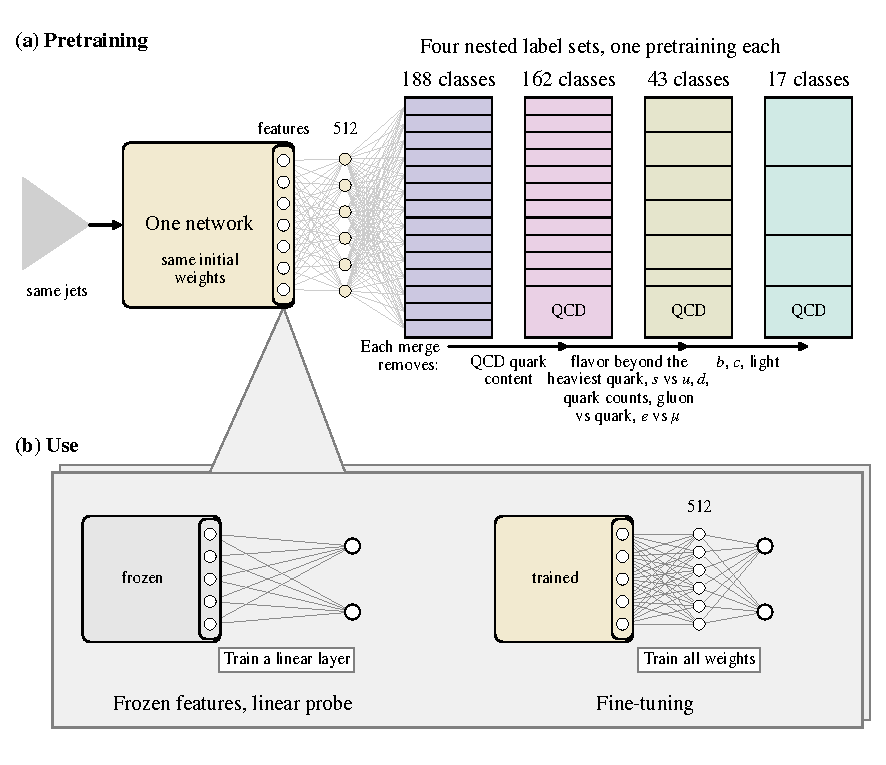
\includegraphics{../../figures/round4/F1.pdf}
\caption{Panel (a) shows six JetClass-II classes as schematic jets (tracks as lines, calorimeter deposits as grey cells) above their fine (188-class) and coarse (17-class) labels, and below, each row a label set and each bar a merged class. Panel (b) shows the network, the Particle Transformer architecture with Sophon's output head, pretrained from scratch for each label set on the same jets in the same order. Each pretrained network is used frozen (open squares) or fine-tuned (filled) on five tasks, JetClass-II, JetClass, top tagging, quark/gluon tagging, and $X\to b\bar b$ and $X\to bs$ resonance tagging, the last frozen only. A label set has three pretraining runs, and the networks with an added mass regression (+ mass) and the 17-class partitions of later figures have two, except the five random partitions with one each (table 1).}\label{fig:F1}
\end{figure}
\FloatBarrier
\clearpage
\begin{figure}[H]
\centering
\includegraphics[width=\linewidth]{../../figures/round4/F2.pdf}
\caption{With linear probes, 43 and 17 classes and every 17-class partition are less accurate on JetClass-II than 188 classes. On top and quark/gluon tagging no network differs from 188 classes in $R_{30}$ by more than three standard deviations; in accuracy, R50 and AUC some do (tables A13 and A1). Points are means $\pm$1 standard deviation over the runs of figure 1, over the five random partitions, or over three initializations of the untrained random network, the linear-probe reference, beyond the // breaks in (a) and (b). The released Sophon checkpoint, one network, appears on JetClass-II and JetClass only. $R_{30}$ is the inverse background efficiency at 30\% signal efficiency, and quark/gluon tagging trains on Pythia jets. Values are in table 1, figure 3 shows the fine-tuned networks and table A1 the area under the receiver operating characteristic curve.}\label{fig:F2}
\end{figure}
\FloatBarrier
\clearpage
\begin{figure}[H]
\centering
\includegraphics[width=\linewidth]{../../figures/round4/F2-ft.pdf}
\caption{After fine-tuning, 17 classes stay below 188 classes on JetClass-II and make about 3\% more errors on JetClass. On top and quark/gluon tagging no network differs from 188 classes in $R_{30}$ by more than three standard deviations; in AUC one does (table A1). Points are means $\pm$1 standard deviation over the runs of figure 1, over the five random partitions, or over three trainings from scratch, the fine-tuned reference. $R_{30}$ is the inverse background efficiency at 30\% signal efficiency, and quark/gluon tagging trains on Pythia jets. Values are in table 1, figure 2 shows the linear probes and table A1 the area under the receiver operating characteristic curve.}\label{fig:F2-ft}
\end{figure}
\FloatBarrier
\clearpage
\begin{figure}[H]
\centering
\includegraphics[width=\linewidth]{../../figures/round4/PC-jc2.pdf}
\caption{Beyond three standard deviations of the spread over runs and test jets, 162, 43 and 17 classes, 162 classes + mass and 17 classes + mass have a lower recall than 188 classes on 13, 127 and 164 of the 188 JetClass-II classes as linear probes (13 of the 162-class ones QCD classes), and a higher one on 1 in all. Each point is one JetClass-II class's recall, the fraction of its test jets the network assigns to it, for the panel's network (vertical) against 188 classes (horizontal), as linear probes (left) or fine-tuned (right) on one million class-balanced jets; rows are 162, 43 and 17 classes, and points below the dotted diagonal are classes the panel's network recalls less often. Averaged with each class's test jets, the recalls give the accuracy of figures 2 and 3. Points are means over three pretraining runs with bars of $\pm$1 standard deviation over runs and test jets, colored by what the 17-class labels merge the class with: decays differing only in quark flavor, only in lepton flavor, both or neither, and the QCD classes. Values are in the supplementary material.}\label{fig:PC-jc2}
\end{figure}
\FloatBarrier
\clearpage
\begin{figure}[H]
\centering
\includegraphics[width=\linewidth]{../../figures/round4/F4-mech.pdf}
\caption{Linear probes on 17 classes separate decays differing only in quark flavor worse than 188 classes; the $b$-quark boundary recovers part of the loss on both pairs, and the random flavor boundary on $X\to bc$ vs $bq$, $cs$. Panels show background rejection against signal efficiency for the label sets and mass networks (upper row) and the flavor-boundary partitions (lower row), means over the runs of figure 1 down to 20 background jets. Lower panels give ratios to 188 classes on a logarithmic axis, banded for 188 classes only by run spread and binomial uncertainty. Random partitions, which merge the pair's classes differently, are in the supplementary material. Figure A3 shows the fine-tuned networks, and table A10 the values and other spreads.}\label{fig:F4-mech}
\end{figure}
\FloatBarrier
\clearpage
\begin{figure}[H]
\centering
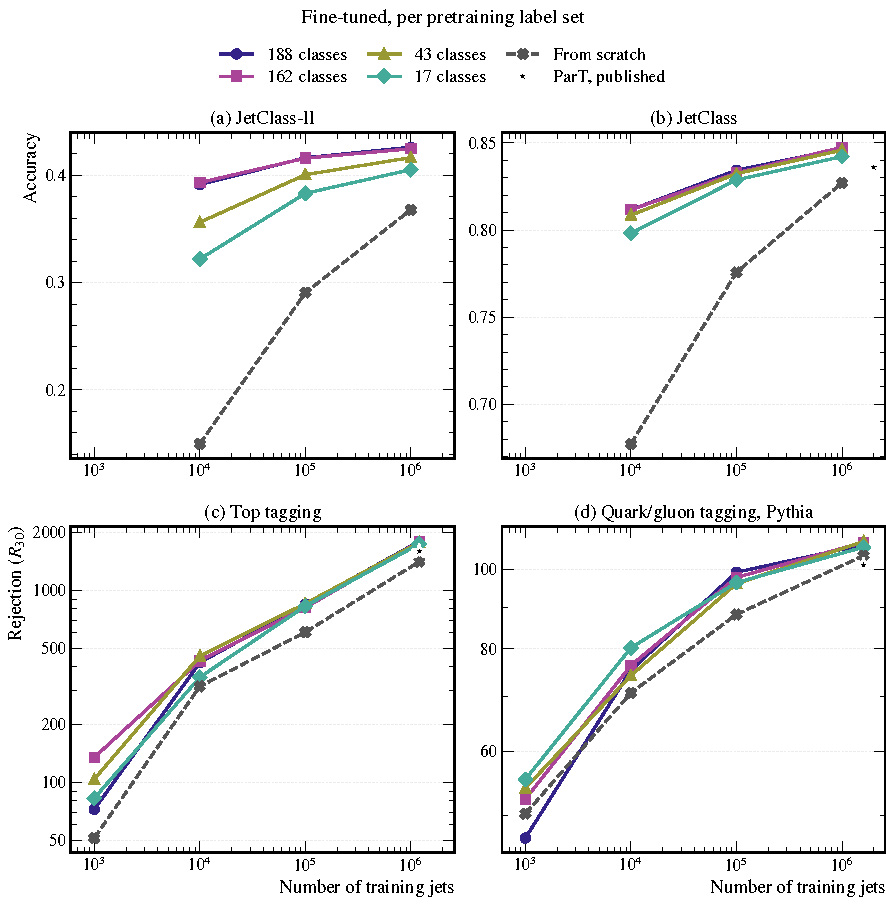
\includegraphics[height=18.5cm]{../../figures/round4/A8.pdf}
\caption{After fine-tuning, 17 classes are less accurate than 188 classes on JetClass-II at every training-set size and on JetClass at one million jets, while on top and quark/gluon tagging, Pythia and Herwig, no label set or mass network differs from 188 classes in $R_{30}$ by more than three standard deviations. The upper panels show accuracy and $R_{30}$, the inverse background efficiency at 30\% signal efficiency, and the lower panels the area under the ROC curve, averaged over the classes on JetClass-II and JetClass. Error bars are $\pm$1 standard deviation over the runs of figure 1 or three trainings from scratch (grey); open stars mark the published Particle Transformer. Figure A6 shows the linear probes, and values are in tables A12 and 1.}\label{fig:A8}
\end{figure}
\FloatBarrier
\begin{figure}[H]
\centering
\includegraphics[width=\linewidth]{../../figures/round4/F11.pdf}
\caption{At 1\% QCD efficiency, 17 classes keep fewer $X\to b\bar b$ and $X\to bs$ jets than 188 classes, a gap of 0.6 and 1.0 in the figure of merit, which widens below 0.1\% for $X\to bs$. The figure of merit, signal efficiency over the square root of QCD efficiency, is shown for (a) $X\to b\bar b$ and (b) $X\to bs$ against QCD, all jets with soft-drop mass 150 to 230 GeV and efficiencies relative to them. Solid curves are a multilayer-perceptron classifier on frozen features starting from the pretrained output head, grey curves training from scratch, and dash-dotted curves the $X\to b\bar b$ output against the QCD outputs (188, 162 and 162 classes + mass, in (a)). Bands, for 188 classes and from scratch only, are $\pm$1 standard deviation over the runs of figure 1 or three trainings. Table 4 holds the values.}\label{fig:F11}
\end{figure}
\FloatBarrier
% tables/mlst_summary.tex
\begin{landscape}
{
\setlength{\LTleft}{0pt}\setlength{\LTright}{0pt}\setlength{\LTcapwidth}{\linewidth}\makeatletter\def\LT@makecaption#1#2#3{\LT@mcol\LT@cols c{\hbox to\z@{\hss\parbox[t]\LTcapwidth{\normalsize #1{#2. }#3\par\vskip\belowcaptionskip}\hss}}}\makeatother
\setlength{\tabcolsep}{6pt}
\begin{center}
\begin{minipage}{\linewidth}\centering
\setlength{\abovecaptionskip}{0pt}
\captionof{table}{Accuracy on class-balanced JetClass-II (at most 5,000 test jets a class) and JetClass and $R_{30}$, the inverse background efficiency at 30\% signal efficiency, on top and quark/gluon tagging, of linear probes and fine-tuned networks. The released Sophon checkpoint's zero-filled top and quark/gluon probes are in table~\ref{tab:probes}. In $R_{30}$ on top and quark/gluon tagging no pretrained network, as a linear probe or fine-tuned, differs from \Kfull{} classes by more than three standard deviations of the runs and the test jets, nor a mass network from its own label set. Values are the mean $\pm$ standard deviation over \MlstNRunsWord{} runs, \MlstMassNRunsWord{} per mass network and flavor-boundary partition, and over five random partitions. Bold marks the best value in their column under their italic heading and those within three standard deviations (run spreads and any stored test-jet bootstrap). References (random network, released Sophon checkpoint, from scratch) are never bold. $^{\S}$~marks a value from a single run.}
\label{tab:summary}
\par\medskip
\begin{tabular*}{\linewidth}{@{\extracolsep{\fill}}lccccc@{}}
\toprule
 & JetClass-II & JetClass & top tagging & \multicolumn{2}{c}{quark/gluon tagging} \\
\cmidrule(lr){5-6}
 & accuracy & accuracy & $R_{30}$ & $R_{30}$, Pythia & $R_{30}$, Herwig \\
\midrule
\multicolumn{6}{@{}l}{\textit{linear probe on the frozen features}} \\
\Kfull{} classes & {\fontseries{b}\selectfont 0.43476\,$\pm$\,0.00035} & {\fontseries{b}\selectfont 0.7709\,$\pm$\,0.0023} & {\fontseries{b}\selectfont 228\,$\pm$\,25} & {\fontseries{b}\selectfont 72.8\,$\pm$\,2.4} & {\fontseries{b}\selectfont 35.0\,$\pm$\,2.6} \\
\Kres{} classes & {\fontseries{b}\selectfont 0.4328\,$\pm$\,0.0008} & {\fontseries{b}\selectfont 0.7709\,$\pm$\,0.0005} & {\fontseries{b}\selectfont 199\,$\pm$\,25} & {\fontseries{b}\selectfont 70.97\,$\pm$\,0.28} & {\fontseries{b}\selectfont 35.9\,$\pm$\,1.7} \\
\Kres{} classes + mass & {\fontseries{b}\selectfont 0.4288\,$\pm$\,0.0024} & {\fontseries{b}\selectfont 0.7739\,$\pm$\,0.0030} & {\fontseries{b}\selectfont 283\,$\pm$\,33} & {\fontseries{b}\selectfont 72.3\,$\pm$\,2.3} & {\fontseries{b}\selectfont 35.3\,$\pm$\,0.5} \\
\Kmid{} classes & 0.361\,$\pm$\,0.005 & {\fontseries{b}\selectfont 0.7695\,$\pm$\,0.0014} & {\fontseries{b}\selectfont 231\,$\pm$\,8} & {\fontseries{b}\selectfont 70.8\,$\pm$\,1.8} & {\fontseries{b}\selectfont 34.4\,$\pm$\,1.7} \\
\Kcoarse{} classes & 0.334\,$\pm$\,0.007 & 0.7606\,$\pm$\,0.0027 & {\fontseries{b}\selectfont 255\,$\pm$\,17} & {\fontseries{b}\selectfont 74.3\,$\pm$\,2.0} & {\fontseries{b}\selectfont 35.5\,$\pm$\,1.0} \\
\Kcoarse{} classes + mass & 0.331\,$\pm$\,0.026 & 0.7618\,$\pm$\,0.0009 & {\fontseries{b}\selectfont 340\,$\pm$\,50} & {\fontseries{b}\selectfont 70.2\,$\pm$\,3.0} & {\fontseries{b}\selectfont 35.5\,$\pm$\,1.2} \\
\multicolumn{6}{@{}l}{\textit{17-class partitions}} \\
\quad no flavor boundary & 0.3746\,$\pm$\,0.0033 & 0.7511\,$\pm$\,0.0034 & {\fontseries{b}\selectfont 253\,$\pm$\,13} & {\fontseries{b}\selectfont 72.8\,$\pm$\,1.5} & {\fontseries{b}\selectfont 34.6\,$\pm$\,0.4} \\
\quad $b$-quark boundary & 0.3954\,$\pm$\,0.0013 & 0.7630\,$\pm$\,0.0021 & {\fontseries{b}\selectfont 207\,$\pm$\,6} & {\fontseries{b}\selectfont 72.36\,$\pm$\,0.22} & {\fontseries{b}\selectfont 34.9\,$\pm$\,0.5} \\
\quad random flavor boundary & 0.4080\,$\pm$\,0.0013 & 0.7579\,$\pm$\,0.0021 & {\fontseries{b}\selectfont 224\,$\pm$\,13} & {\fontseries{b}\selectfont 72.0\,$\pm$\,1.2} & {\fontseries{b}\selectfont 35.3\,$\pm$\,0.4} \\
\quad random partitions & 0.4215\,$\pm$\,0.0014 & 0.7541\,$\pm$\,0.0009 & 163\,$\pm$\,11 & {\fontseries{b}\selectfont 68.3\,$\pm$\,2.1} & {\fontseries{b}\selectfont 34.0\,$\pm$\,1.4} \\
random network & 0.0724\,$\pm$\,0.0015 & 0.4077\,$\pm$\,0.0013 & 56.8\,$\pm$\,2.8 & 56.4\,$\pm$\,1.0 & 31.6\,$\pm$\,0.8 \\
\midrule
released Sophon checkpoint & 0.4340$^{\S}$ & 0.7679$^{\S}$ & -- & -- & -- \\
\bottomrule
\end{tabular*}
\end{minipage}
\end{center}
\newpage
\begin{center}
\begin{minipage}{\linewidth}\centering
\makebox[\linewidth][l]{\textit{Table~\ref{tab:summary} (continued)}}
\par\smallskip
\begin{tabular*}{\linewidth}{@{\extracolsep{\fill}}lccccc@{}}
\toprule
 & JetClass-II & JetClass & top tagging & \multicolumn{2}{c}{quark/gluon tagging} \\
\cmidrule(lr){5-6}
 & accuracy & accuracy & $R_{30}$ & $R_{30}$, Pythia & $R_{30}$, Herwig \\
\midrule
\multicolumn{6}{@{}l}{\textit{fine-tuned}} \\
\Kfull{} classes & -- & -- & {\fontseries{b}\selectfont 1{,}800\,$\pm$\,60} & {\fontseries{b}\selectfont 107.3\,$\pm$\,2.2} & {\fontseries{b}\selectfont 35.2\,$\pm$\,2.1} \\
\Kres{} classes & -- & -- & {\fontseries{b}\selectfont 1{,}790\,$\pm$\,60} & {\fontseries{b}\selectfont 108.0\,$\pm$\,1.4} & {\fontseries{b}\selectfont 34.6\,$\pm$\,2.0} \\
\Kres{} classes + mass & -- & -- & {\fontseries{b}\selectfont 1{,}770\,$\pm$\,250} & {\fontseries{b}\selectfont 106.78\,$\pm$\,0.24} & {\fontseries{b}\selectfont 36.1\,$\pm$\,2.4} \\
\Kmid{} classes & -- & -- & {\fontseries{b}\selectfont 1{,}780\,$\pm$\,150} & {\fontseries{b}\selectfont 108.3\,$\pm$\,1.0} & {\fontseries{b}\selectfont 36.1\,$\pm$\,2.7} \\
\Kcoarse{} classes & -- & -- & {\fontseries{b}\selectfont 1{,}740\,$\pm$\,140} & {\fontseries{b}\selectfont 106.5\,$\pm$\,0.8} & {\fontseries{b}\selectfont 36.9\,$\pm$\,0.9} \\
\Kcoarse{} classes + mass & -- & -- & {\fontseries{b}\selectfont 1{,}660\,$\pm$\,40} & {\fontseries{b}\selectfont 105.3\,$\pm$\,0.5} & {\fontseries{b}\selectfont 35.3\,$\pm$\,3.4} \\
\multicolumn{6}{@{}l}{\textit{17-class partitions}} \\
\quad no flavor boundary & -- & -- & {\fontseries{b}\selectfont 1{,}790\,$\pm$\,90} & {\fontseries{b}\selectfont 109.05\,$\pm$\,0.17} & {\fontseries{b}\selectfont 37\,$\pm$\,4} \\
\quad $b$-quark boundary & -- & -- & {\fontseries{b}\selectfont 1{,}830\,$\pm$\,330} & 106.67\,$\pm$\,0.24 & {\fontseries{b}\selectfont 36.4\,$\pm$\,2.4} \\
\quad random flavor boundary & -- & -- & {\fontseries{b}\selectfont 1{,}610\,$\pm$\,60} & {\fontseries{b}\selectfont 106.3\,$\pm$\,2.7} & {\fontseries{b}\selectfont 36.2\,$\pm$\,1.8} \\
\quad random partitions & -- & -- & {\fontseries{b}\selectfont 1{,}750\,$\pm$\,110} & {\fontseries{b}\selectfont 107.0\,$\pm$\,1.0} & {\fontseries{b}\selectfont 35.2\,$\pm$\,1.5} \\
from scratch & -- & -- & 1{,}412\,$\pm$\,20 & 104.0\,$\pm$\,1.0 & 35.5\,$\pm$\,1.2 \\
\bottomrule
\end{tabular*}
\end{minipage}
\end{center}
\par\smallskip{\noindent A network marked + mass has an added jet-mass regression output; the 17-class partitions regroup the 188 classes into 17, and the random partitions are the 161 resonant classes split at random into 16 groups, with QCD kept as the 17th.}
}
\end{landscape}
\FloatBarrier
% tables/mlst_published.tex
\begin{landscape}
{
\setlength{\LTleft}{0pt}\setlength{\LTright}{0pt}\setlength{\LTcapwidth}{\linewidth}\makeatletter\def\LT@makecaption#1#2#3{\LT@mcol\LT@cols c{\hbox to\z@{\hss\parbox[t]\LTcapwidth{\normalsize #1{#2. }#3\par\vskip\belowcaptionskip}\hss}}}\makeatother
\setlength{\tabcolsep}{6pt}
\begin{center}
\begin{minipage}{\linewidth}\centering
\setlength{\abovecaptionskip}{0pt}
\captionof{table}{Published models beside ours, the mean $\pm$ standard deviation over three runs. Models marked fine-tuned and OmniLearned are pretrained on other data, training jets counting the downstream set. AUC is the area under the receiver operating characteristic curve, on JetClass averaged over the classes, each against the rest, equal here to ParT's average over class pairs. $R_{50}$ and $R_{30}$ are inverse background efficiencies at 50\% and 30\% signal efficiency. Bold marks the best value in their column and task and those within three standard deviations (run spreads and any stored test-jet bootstrap). A published value without an uncertainty is never bold. The kinematic-inputs network is a reference, never bold. $^{\S}$~marks a value from a single run.}
\label{tab:published}
\par\medskip
\begin{tabular*}{\linewidth}{@{\extracolsep{\fill}}lcccccc@{}}
\toprule
 & parameters & training jets & accuracy & AUC & $R_{50}$ & $R_{30}$ \\
\midrule
\multicolumn{7}{@{}l}{JetClass} \\
ParticleNet & 366\,k & 2\,M & 0.828 & 0.9820 & -- & -- \\
ParT & 2.14\,M & 2\,M & 0.836 & 0.9834 & -- & -- \\
from scratch (this work) & 2.21\,M & 1\,M & 0.8267\,$\pm$\,0.0011 & 0.98177\,$\pm$\,0.00026 & -- & -- \\
fine-tuned from \Kfull{} classes (this work) & 2.21\,M & 1\,M & {\fontseries{b}\selectfont 0.8468\,$\pm$\,0.0006} & {\fontseries{b}\selectfont 0.98538\,$\pm$\,0.00007} & -- & -- \\
\midrule
\multicolumn{7}{@{}l}{top tagging} \\
linear EFP & 1\,k & 1.2\,M & 0.932 & 0.980 & -- & 384 \\
ParticleNet & 366\,k & 1.2\,M & 0.940 & 0.9858 & 397\,$\pm$\,7 & 1{,}615\,$\pm$\,93 \\
ParT & 2.14\,M & 1.2\,M & 0.940 & 0.9858 & 413\,$\pm$\,16 & 1{,}602\,$\pm$\,81 \\
ParT, fine-tuned & 2.14\,M & 1.2\,M & 0.944 & 0.9877 & {\fontseries{b}\selectfont 691\,$\pm$\,15} & 2{,}766\,$\pm$\,130 \\
MIParT-L, fine-tuned & 2.38\,M & 1.2\,M & 0.944 & 0.9878 & {\fontseries{b}\selectfont 640\,$\pm$\,10} & 2{,}789\,$\pm$\,133 \\
L-GATr, fine-tuned & 1.1\,M & 1.2\,M & 0.9446 & 0.9879 & {\fontseries{b}\selectfont 651\,$\pm$\,11} & 2{,}894\,$\pm$\,84 \\
OmniLearned-l & 423\,M & 1.2\,M & 0.944 & 0.9880 & {\fontseries{b}\selectfont 688\,$\pm$\,9} & {\fontseries{b}\selectfont 3{,}486\,$\pm$\,157} \\
from scratch (this work) & 2.21\,M & 1.2\,M & 0.93875\,$\pm$\,0.00016 & 0.98524\,$\pm$\,0.00008 & 358\,$\pm$\,11 & 1{,}412\,$\pm$\,20 \\
fine-tuned from \Kfull{} classes (this work) & 2.21\,M & 1.2\,M & {\fontseries{b}\selectfont 0.94001\,$\pm$\,0.00023} & {\fontseries{b}\selectfont 0.98606\,$\pm$\,0.00007} & 461\,$\pm$\,4 & 1{,}799\,$\pm$\,56 \\
\Kfull{} classes, kinematic inputs only & 2.21\,M & 1.2\,M & 0.9407$^{\S}$ & 0.98620$^{\S}$ & 443$^{\S}$ & 1{,}803$^{\S}$ \\
\bottomrule
\end{tabular*}
\end{minipage}
\end{center}
\newpage
\begin{center}
\begin{minipage}{\linewidth}\centering
\makebox[\linewidth][l]{\textit{Table~\ref{tab:published} (continued)}}
\par\smallskip
\begin{tabular*}{\linewidth}{@{\extracolsep{\fill}}lcccccc@{}}
\toprule
 & parameters & training jets & accuracy & AUC & $R_{50}$ & $R_{30}$ \\
\midrule
\multicolumn{7}{@{}l}{quark/gluon tagging} \\
constituent multiplicity & -- & -- & -- & 0.8401 & 19.0 & -- \\
linear EFP & -- & 1\,M & -- & 0.8919 & 29.7 & -- \\
PFN-Ex & -- & 1\,M & -- & 0.9005 & 34.7\,$\pm$\,0.4 & -- \\
ParticleNet & 366\,k & 1.6\,M & 0.840 & 0.9116 & 39.8\,$\pm$\,0.2 & 98.6\,$\pm$\,1.3 \\
ParT & 2.14\,M & 1.6\,M & 0.840 & 0.9121 & 41.3\,$\pm$\,0.3 & 101.2\,$\pm$\,1.1 \\
ParticleNet, fine-tuned & 370\,k & 1.6\,M & 0.839 & 0.9115 & 40.1\,$\pm$\,0.2 & 100.3\,$\pm$\,1.0 \\
ParT, fine-tuned & 2.14\,M & 1.6\,M & 0.843 & 0.9151 & 42.4\,$\pm$\,0.2 & {\fontseries{b}\selectfont 107.9\,$\pm$\,0.5} \\
OmniLearned-m & 58\,M & 1.6\,M & 0.845 & 0.9162 & {\fontseries{b}\selectfont 43.2\,$\pm$\,0.1} & {\fontseries{b}\selectfont 111.2\,$\pm$\,1.5} \\
from scratch (this work) & 2.21\,M & 1.6\,M & 0.8397\,$\pm$\,0.0007 & 0.91212\,$\pm$\,0.00022 & 41.47\,$\pm$\,0.29 & 104.0\,$\pm$\,1.0 \\
fine-tuned from \Kfull{} classes (this work) & 2.21\,M & 1.6\,M & {\fontseries{b}\selectfont 0.84329\,$\pm$\,0.00020} & {\fontseries{b}\selectfont 0.91482\,$\pm$\,0.00014} & 42.56\,$\pm$\,0.10 & {\fontseries{b}\selectfont 107.3\,$\pm$\,2.2} \\
\bottomrule
\end{tabular*}
\end{minipage}
\end{center}
\par\smallskip{\noindent A dash marks a value not reported or not applicable.}
}
\end{landscape}
\FloatBarrier
% tables/mlst_mass.tex
\begin{center}
\begin{minipage}{\linewidth}\centering
\centering
\captionof{table}{Jet-mass resolution and median response of $r = m/m_{\mathrm{gen}}$, the estimated mass over the generator-level soft-drop mass, on JetClass-II test jets with a generator-level match, for the soft-drop mass, the mass output of the pretraining head and a multilayer-perceptron probe on the frozen features. The resolution is half the 15.9--84.1\% quantile range of $r$ over its median. The probe is centred on one training median, with no generator truth. The best resolution is the smallest and the best median response the closest to one. Values are the mean $\pm$ standard deviation over \MlstNRunsWord{} runs, \MlstMassNRunsWord{} per mass network. Bold marks the best value in their column under their italic heading and those within three standard deviations (run spreads and any stored test-jet bootstrap). References (random network, soft-drop mass) are never bold.}
\label{tab:mass}
\begin{tabular*}{\linewidth}{@{\extracolsep{\fill}}lcc@{}}
\toprule
 & resolution & median response \\
\midrule
\multicolumn{3}{@{}l}{\textit{mass output of the pretraining head}} \\
\Kres{} classes + mass & {\fontseries{b}\selectfont 0.1467\,$\pm$\,0.0006} & {\fontseries{b}\selectfont 0.999\,$\pm$\,0.005} \\
\Kcoarse{} classes + mass & {\fontseries{b}\selectfont 0.1455\,$\pm$\,0.0008} & {\fontseries{b}\selectfont 1.00523\,$\pm$\,0.00019} \\
\midrule
\multicolumn{3}{@{}l}{\textit{multilayer-perceptron probe on the frozen features}} \\
\Kfull{} classes & 0.2181\,$\pm$\,0.0019 & {\fontseries{b}\selectfont 0.9919\,$\pm$\,0.0021} \\
\Kres{} classes & 0.2173\,$\pm$\,0.0016 & {\fontseries{b}\selectfont 0.992\,$\pm$\,0.004} \\
\Kres{} classes + mass & 0.15726\,$\pm$\,0.00003 & {\fontseries{b}\selectfont 1.0085\,$\pm$\,0.0024} \\
\Kmid{} classes & 0.2145\,$\pm$\,0.0034 & {\fontseries{b}\selectfont 0.993\,$\pm$\,0.005} \\
\Kcoarse{} classes & 0.2082\,$\pm$\,0.0023 & {\fontseries{b}\selectfont 0.9929\,$\pm$\,0.0033} \\
\Kcoarse{} classes + mass & {\fontseries{b}\selectfont 0.15584\,$\pm$\,0.00023} & {\fontseries{b}\selectfont 1.008\,$\pm$\,0.006} \\
random network & 0.2399\,$\pm$\,0.0031 & 0.9815\,$\pm$\,0.0013 \\
\midrule
soft-drop mass & 0.2448\,$\pm$\,0.0006 & 0.9294\,$\pm$\,0.0004 \\
\bottomrule
\end{tabular*}
\end{minipage}
\end{center}
\FloatBarrier
% tables/mlst_xbx.tex
\begin{landscape}
{
\setlength{\LTleft}{0pt}\setlength{\LTright}{0pt}\setlength{\LTcapwidth}{\linewidth}\makeatletter\def\LT@makecaption#1#2#3{\LT@mcol\LT@cols c{\hbox to\z@{\hss\parbox[t]\LTcapwidth{\normalsize #1{#2. }#3\par\vskip\belowcaptionskip}\hss}}}\makeatother
\begin{center}
\begin{minipage}{\linewidth}\centering
\setlength{\abovecaptionskip}{0pt}
\captionof{table}{Signal efficiency in percent of $X\to b\bar b$ and $X\to bs$ jets against QCD jets at the QCD efficiency $\varepsilon_B$ in the header, relative to the jets with soft-drop mass \XbxWindowLo--\XbxWindowHi~GeV. The pretrained networks, not fine-tuned, are read out on frozen features by a multilayer-perceptron classifier starting from their output head or by a linear probe, or directly by the $X\to b\bar b$ output against the QCD outputs. From scratch trains on each signal, and a dash marks a read-out a network lacks. Values are the mean $\pm$ standard deviation over \MlstNRunsWord{} runs, \MlstMassNRunsWord{} per mass network and flavor-boundary partition, and over five random partitions. Bold marks the best value in their column and those within three standard deviations (run spreads and any stored test-jet bootstrap). References (random network, from scratch) are never bold.}
\label{tab:xbx}
\par\medskip
\begin{tabular*}{\linewidth}{@{\extracolsep{\fill}}lccccc@{}}
\toprule
 & \multicolumn{5}{c}{signal efficiency (\%) at $\varepsilon_B=0.01$} \\
\cmidrule(lr){2-6}
 & \multicolumn{3}{c}{$X\to b\bar b$} & \multicolumn{2}{c}{$X\to bs$} \\
\cmidrule(lr){2-4}\cmidrule(lr){5-6}
pretraining & classifier & linear probe & direct & classifier & linear probe \\
\midrule
\Kfull{} classes & {\fontseries{b}\selectfont 71.79\,$\pm$\,0.14} & {\fontseries{b}\selectfont 70.9\,$\pm$\,0.5} & {\fontseries{b}\selectfont 69.84\,$\pm$\,0.05} & {\fontseries{b}\selectfont 69.22\,$\pm$\,0.19} & {\fontseries{b}\selectfont 66.56\,$\pm$\,0.10} \\
\Kres{} classes & {\fontseries{b}\selectfont 71.69\,$\pm$\,0.27} & {\fontseries{b}\selectfont 69.7\,$\pm$\,0.4} & {\fontseries{b}\selectfont 69.95\,$\pm$\,0.19} & {\fontseries{b}\selectfont 68.90\,$\pm$\,0.06} & {\fontseries{b}\selectfont 65.4\,$\pm$\,0.9} \\
\Kres{} classes + mass & {\fontseries{b}\selectfont 71.1\,$\pm$\,0.5} & {\fontseries{b}\selectfont 70.1\,$\pm$\,1.2} & {\fontseries{b}\selectfont 69.71\,$\pm$\,0.21} & 68.03\,$\pm$\,0.05 & {\fontseries{b}\selectfont 64.6\,$\pm$\,0.7} \\
\Kmid{} classes & {\fontseries{b}\selectfont 70.81\,$\pm$\,0.33} & {\fontseries{b}\selectfont 69.2\,$\pm$\,0.6} & -- & 67.14\,$\pm$\,0.07 & 64.59\,$\pm$\,0.18 \\
\Kcoarse{} classes & 65.9\,$\pm$\,1.0 & 67.0\,$\pm$\,1.1 & -- & 59.4\,$\pm$\,1.6 & 58.6\,$\pm$\,2.0 \\
\Kcoarse{} classes + mass & 66.78\,$\pm$\,0.25 & {\fontseries{b}\selectfont 68.3\,$\pm$\,1.8} & -- & 59.9\,$\pm$\,1.2 & 59.6\,$\pm$\,1.0 \\
\multicolumn{6}{@{}l}{\textit{17-class partitions}} \\
\quad no flavor boundary & 62.5\,$\pm$\,0.8 & 63.3\,$\pm$\,0.4 & -- & 59.30\,$\pm$\,0.29 & 58.7\,$\pm$\,1.6 \\
\quad $b$-quark boundary & 67.3\,$\pm$\,0.5 & 67.3\,$\pm$\,0.9 & -- & 61.6\,$\pm$\,0.5 & 60.076\,$\pm$\,0.017 \\
\quad random flavor boundary & 66.89\,$\pm$\,0.27 & {\fontseries{b}\selectfont 65.8\,$\pm$\,2.2} & -- & 63.20\,$\pm$\,0.27 & 60.7\,$\pm$\,0.7 \\
\quad random partitions & 69.1\,$\pm$\,0.8 & {\fontseries{b}\selectfont 68.3\,$\pm$\,1.8} & -- & 65.1\,$\pm$\,1.2 & {\fontseries{b}\selectfont 63.2\,$\pm$\,1.2} \\
random network & -- & 18.0\,$\pm$\,1.6 & -- & -- & 13.4\,$\pm$\,0.6 \\
from scratch & 57\,$\pm$\,8 & -- & -- & 55.4\,$\pm$\,1.0 & -- \\
\bottomrule
\end{tabular*}
\end{minipage}
\end{center}
}
\end{landscape}
\FloatBarrier
\clearpage
\setcounter{figure}{0}\setcounter{table}{0}
\renewcommand{\thefigure}{A\arabic{figure}}\renewcommand{\theHfigure}{appendix.\arabic{figure}}
\renewcommand{\thetable}{A\arabic{table}}\renewcommand{\theHtable}{appendix.\arabic{table}}
\noindent\textbf{Where each result is.} Every figure and table of the paper shows the label sets (188, 162, 43 and 17 classes) and the mass networks (162 and 17 classes + mass); the 17-class partitions appear in the paper for the headline metrics, class pairs and resonance tagging, and in the supplementary material for every other family; the per-class and embedding figures show the label sets only. Each cell gives the figures and tables of the paper that show that group of networks in that mode, or says where it is.

\begin{center}\scriptsize\setlength{\tabcolsep}{2.5pt}
\begin{tabular}{@{}>{\raggedright\arraybackslash}p{1.55cm}*{6}{>{\raggedright\arraybackslash}p{2.05cm}}@{}}
\toprule
 & \multicolumn{3}{c}{linear probe or frozen} & \multicolumn{3}{c}{fine-tuned} \\
\cmidrule(lr){2-4}\cmidrule(lr){5-7}
 family & label sets & mass networks & partitions & label sets & mass networks & partitions \\
\midrule
Headline metrics & Fig.~2; Tables 1, A1 & Fig.~2; Tables 1, A1 & Fig.~2; Tables 1, A1 & Fig.~3; Tables 1, 2, A1 & Fig.~3; Tables 1, A1 & Fig.~3; Tables 1, A1 \\
Per class & Fig.~4; Table A4 & Table A4 & supplement & Fig.~4; Tables A4, A6 & Tables A4, A6 & supplement \\
Class pairs & Figs.~5, A1, A2; Table A10 & Figs.~5, A1, A2; Table A10 & Figs.~5, A1, A2; Table A10 & Figs.~A3, A4, A5; Table A10 & Figs.~A3, A4, A5; Table A10 & Figs.~A3, A4, A5; Table A10 \\
Training size & Fig.~A6; Table A11 & Fig.~A6; Table A11 & supplement & Fig.~6; Table A12 & Fig.~6; Table A12 & supplement \\
ROC curves & Fig.~A7; Table A13 & Fig.~A7; Table A13 & supplement & Fig.~A8; Table A14 & Fig.~A8; Table A14 & supplement \\
Jet $p_{\mathrm{T}}$  & Fig.~A9 & Fig.~A9 & supplement & Fig.~A9 & Fig.~A9 & supplement \\
Mass & Fig.~A11; Tables 3, A15 & Figs.~A10, A11; Tables 3, A15 & supplement & Table A15 & Table A15 & does not apply (no network is fine-tuned to regress the jet mass) \\
Sculpting & Fig.~A12; Table A17 & Fig.~A12; Table A17 & supplement & Fig.~A12; Table A17 & Fig.~A12; Table A17 & supplement \\
Resonance tagging & Figs.~7, A13; Tables 4, A19 & Figs.~7, A13; Tables 4, A19 & Fig.~A13; Tables 4, A19 & does not apply (the pretrained networks are not fine-tuned on these samples) & does not apply (the pretrained networks are not fine-tuned on these samples) & does not apply (the pretrained networks are not fine-tuned on these samples) \\
Embeddings & Fig.~A14 & supplement & does not apply (the embeddings compare the label sets) & Fig.~A15 & supplement & does not apply (the embeddings compare the label sets) \\
Training details & Fig.~A16; Table A21 & Fig.~A16; Table A21 & supplement & Fig.~A16; Table A23 & Fig.~A16 & supplement \\
\bottomrule
\end{tabular}
\end{center}
\clearpage
\clearpage
\paragraph*{Headline metrics}\mbox{}

\nopagebreak
% tables/mlst_summary_auc.tex
\begin{landscape}
{
\setlength{\LTleft}{0pt}\setlength{\LTright}{0pt}\setlength{\LTcapwidth}{\linewidth}\makeatletter\def\LT@makecaption#1#2#3{\LT@mcol\LT@cols c{\hbox to\z@{\hss\parbox[t]\LTcapwidth{\normalsize #1{#2. }#3\par\vskip\belowcaptionskip}\hss}}}\makeatother
\setlength{\tabcolsep}{6pt}
\begin{center}
\begin{minipage}{\linewidth}\centering
\setlength{\abovecaptionskip}{0pt}
\captionof{table}{The area under the receiver operating characteristic curve (AUC) of the linear probes and fine-tuned networks of table~\ref{tab:summary}, on the same sets, averaged on JetClass-II and JetClass over the classes, each against the rest. The released Sophon checkpoint's dashes are those of table~\ref{tab:summary}. As linear probes, beyond three standard deviations of the runs and the test jets, \Kcoarse{} classes + mass has a higher AUC than \Kfull{} classes on top tagging and a lower one on Pythia quark/gluon tagging, and the random partitions a lower one on top tagging; no other top or quark/gluon AUC of a linear probe differs from \Kfull{} classes, nor of a mass network from its own label set. Fine-tuned, only \Kcoarse{} classes + mass differs, with a lower AUC on Pythia quark/gluon tagging. Values are the mean $\pm$ standard deviation over \MlstNRunsWord{} runs, \MlstMassNRunsWord{} per mass network and flavor-boundary partition, and over five random partitions. Bold marks the best value in their column under their italic heading and those within three standard deviations (run spreads and any stored test-jet bootstrap). References (random network, released Sophon checkpoint, from scratch) are never bold. $^{\S}$~marks a value from a single run. $^{\P}$~marks a run spread below the last digit shown.}
\label{tab:summaryauc}
\par\medskip
\begin{tabular*}{\linewidth}{@{\extracolsep{\fill}}lccccc@{}}
\toprule
 & JetClass-II & JetClass & top tagging & \multicolumn{2}{c}{quark/gluon tagging} \\
\cmidrule(lr){5-6}
 & AUC & AUC & AUC & AUC, Pythia & AUC, Herwig \\
\midrule
\multicolumn{6}{@{}l}{\textit{linear probe on the frozen features}} \\
\Kfull{} classes & {\fontseries{b}\selectfont 0.98014\,$\pm$\,0.00001} & {\fontseries{b}\selectfont 0.9682\,$\pm$\,0.0006} & 0.9686\,$\pm$\,0.0007 & {\fontseries{b}\selectfont 0.88347\,$\pm$\,0.00016} & {\fontseries{b}\selectfont 0.8075\,$\pm$\,0.0006} \\
\Kres{} classes & 0.97963\,$\pm$\,0.00010 & {\fontseries{b}\selectfont 0.96832\,$\pm$\,0.00016} & 0.9671\,$\pm$\,0.0020 & {\fontseries{b}\selectfont 0.8818\,$\pm$\,0.0018} & {\fontseries{b}\selectfont 0.8068\,$\pm$\,0.0022} \\
\Kres{} classes + mass & 0.97924\,$\pm$\,0.00023 & {\fontseries{b}\selectfont 0.9690\,$\pm$\,0.0009} & {\fontseries{b}\selectfont 0.9709\,$\pm$\,0.0009} & {\fontseries{b}\selectfont 0.8834\,$\pm$\,0.0005} & {\fontseries{b}\selectfont 0.8071\,$\pm$\,0.0010} \\
\Kmid{} classes & 0.97562\,$\pm$\,0.00016 & {\fontseries{b}\selectfont 0.9680\,$\pm$\,0.0004} & 0.9681\,$\pm$\,0.0013 & {\fontseries{b}\selectfont 0.8821\,$\pm$\,0.0011} & {\fontseries{b}\selectfont 0.8058\,$\pm$\,0.0011} \\
\Kcoarse{} classes & 0.9691\,$\pm$\,0.0004 & 0.9650\,$\pm$\,0.0008 & {\fontseries{b}\selectfont 0.9710\,$\pm$\,0.0006} & {\fontseries{b}\selectfont 0.8821\,$\pm$\,0.0015} & {\fontseries{b}\selectfont 0.8053\,$\pm$\,0.0020} \\
\Kcoarse{} classes + mass & 0.9688\,$\pm$\,0.0013 & 0.96532\,$\pm$\,0.00026 & {\fontseries{b}\selectfont 0.9741\,$\pm$\,0.0010} & {\fontseries{b}\selectfont 0.8801\,$\pm$\,0.0006} & {\fontseries{b}\selectfont 0.80794\,$\pm$\,0.00009} \\
\multicolumn{6}{@{}l}{\textit{17-class partitions}} \\
\quad no flavor boundary & 0.9713\,$\pm$\,0.0005 & 0.9628\,$\pm$\,0.0008 & {\fontseries{b}\selectfont 0.9696\,$\pm$\,0.0018} & {\fontseries{b}\selectfont 0.8798\,$\pm$\,0.0035} & {\fontseries{b}\selectfont 0.80569\,$\pm$\,0.00021} \\
\quad $b$-quark boundary & 0.97586\,$\pm$\,0.00010 & {\fontseries{b}\selectfont 0.96629\,$\pm$\,0.00029} & 0.9665\,$\pm$\,0.0011 & {\fontseries{b}\selectfont 0.8805\,$\pm$\,0.0012} & {\fontseries{b}\selectfont 0.80583\,$\pm$\,0.00024} \\
\quad random flavor boundary & 0.97602\,$\pm$\,0.00002 & 0.9649\,$\pm$\,0.0006 & 0.96725\,$\pm$\,0.00023 & {\fontseries{b}\selectfont 0.8818\,$\pm$\,0.0016} & {\fontseries{b}\selectfont 0.80625\,$\pm$\,0.00032} \\
\quad random partitions & 0.97765\,$\pm$\,0.00017 & 0.96379\,$\pm$\,0.00021 & 0.9626\,$\pm$\,0.0019 & {\fontseries{b}\selectfont 0.8788\,$\pm$\,0.0024} & {\fontseries{b}\selectfont 0.8046\,$\pm$\,0.0025} \\
random network & 0.8121\,$\pm$\,0.0019 & 0.8280\,$\pm$\,0.0011 & 0.9408\,$\pm$\,0.0012 & 0.8612\,$\pm$\,0.0016 & 0.7965\,$\pm$\,0.0009 \\
\midrule
released Sophon checkpoint & 0.97990$^{\S}$ & 0.9675$^{\S}$ & -- & -- & -- \\
\bottomrule
\end{tabular*}
\end{minipage}
\end{center}
\newpage
\begin{center}
\begin{minipage}{\linewidth}\centering
\makebox[\linewidth][l]{\textit{Table~\ref{tab:summaryauc} (continued)}}
\par\smallskip
\begin{tabular*}{\linewidth}{@{\extracolsep{\fill}}lccccc@{}}
\toprule
 & JetClass-II & JetClass & top tagging & \multicolumn{2}{c}{quark/gluon tagging} \\
\cmidrule(lr){5-6}
 & AUC & AUC & AUC & AUC, Pythia & AUC, Herwig \\
\midrule
\multicolumn{6}{@{}l}{\textit{fine-tuned}} \\
\Kfull{} classes & -- & -- & {\fontseries{b}\selectfont 0.98606\,$\pm$\,0.00007} & {\fontseries{b}\selectfont 0.91482\,$\pm$\,0.00014} & {\fontseries{b}\selectfont 0.8078\,$\pm$\,0.0023} \\
\Kres{} classes & -- & -- & {\fontseries{b}\selectfont 0.98610\,$\pm$\,0.00008} & {\fontseries{b}\selectfont 0.91478\,$\pm$\,0.00008} & {\fontseries{b}\selectfont 0.8074\,$\pm$\,0.0010} \\
\Kres{} classes + mass & -- & -- & {\fontseries{b}\selectfont 0.98603\,$\pm$\,0.00003} & {\fontseries{b}\selectfont 0.91461\,$\pm$\,0.00011} & {\fontseries{b}\selectfont 0.8091\,$\pm$\,0.0025} \\
\Kmid{} classes & -- & -- & {\fontseries{b}\selectfont 0.98610\,$\pm$\,0.00005} & {\fontseries{b}\selectfont 0.91456\,$\pm$\,0.00032} & {\fontseries{b}\selectfont 0.809\,$\pm$\,0.005} \\
\Kcoarse{} classes & -- & -- & {\fontseries{b}\selectfont 0.98590\,$\pm$\,0.00006} & {\fontseries{b}\selectfont 0.91440\,$\pm$\,0.00003} & {\fontseries{b}\selectfont 0.8103\,$\pm$\,0.0018} \\
\Kcoarse{} classes + mass & -- & -- & {\fontseries{b}\selectfont 0.98583\,$\pm$\,0.00007} & {\fontseries{b}\selectfont 0.91409\,$\pm$\,0.00013} & {\fontseries{b}\selectfont 0.8076\,$\pm$\,0.0034} \\
\multicolumn{6}{@{}l}{\textit{17-class partitions}} \\
\quad no flavor boundary & -- & -- & {\fontseries{b}\selectfont 0.98604\,$\pm$\,0.00007} & {\fontseries{b}\selectfont 0.91446\,$\pm$\,0.00013} & {\fontseries{b}\selectfont 0.8070\,$\pm$\,0.0034} \\
\quad $b$-quark boundary & -- & -- & {\fontseries{b}\selectfont 0.98604\,$\pm$\,0.00007} & {\fontseries{b}\selectfont 0.91472}$^{\P}$ & {\fontseries{b}\selectfont 0.8087\,$\pm$\,0.0030} \\
\quad random flavor boundary & -- & -- & {\fontseries{b}\selectfont 0.98597\,$\pm$\,0.00019} & {\fontseries{b}\selectfont 0.91460\,$\pm$\,0.00016} & {\fontseries{b}\selectfont 0.808\,$\pm$\,0.004} \\
\quad random partitions & -- & -- & {\fontseries{b}\selectfont 0.98598\,$\pm$\,0.00009} & {\fontseries{b}\selectfont 0.91459\,$\pm$\,0.00009} & {\fontseries{b}\selectfont 0.8078\,$\pm$\,0.0007} \\
from scratch & -- & -- & 0.98524\,$\pm$\,0.00008 & 0.91212\,$\pm$\,0.00022 & 0.8061\,$\pm$\,0.0007 \\
\bottomrule
\end{tabular*}
\end{minipage}
\end{center}
}
\end{landscape}
\FloatBarrier
% tables/mlst_mlp.tex
\begin{landscape}
{
\setlength{\LTleft}{0pt}\setlength{\LTright}{0pt}\setlength{\LTcapwidth}{\linewidth}\makeatletter\def\LT@makecaption#1#2#3{\LT@mcol\LT@cols c{\hbox to\z@{\hss\parbox[t]\LTcapwidth{\normalsize #1{#2. }#3\par\vskip\belowcaptionskip}\hss}}}\makeatother
\addtolength{\belowcaptionskip}{\medskipamount}
\begin{longtable}{@{\extracolsep{\fill}}lcccc@{}}
\caption{Multilayer-perceptron probes, with one hidden layer of \LpMlpHidden{} units, on the frozen features of every pretrained network and of the random networks, at each task's largest training set, scored on the AUC for JetClass-II and JetClass, on the AUC and $R_{30}$ for top and quark/gluon tagging, and on the AUC of the class pairs of table~\ref{tab:pairs}. On JetClass-II the mass networks and the random partitions were probed only on its mixed test sample (the last block, beside the four label sets), and the other partitions and the random network only on the class-balanced set. The linear-probe block gives the \Kfull-class networks on the class token and on the pretraining head's 512-unit hidden layer, on JetClass-II and Pythia quark/gluon jets only, as the hidden layer was not scored on Herwig jets. The network on kinematic inputs only is probed on top tagging only. AUC is the area under the receiver operating characteristic curve, averaged over the classes, each against the rest, or over the resonant or the QCD classes only (AUC, resonant and AUC, QCD). $\rho$ is $1-\mathrm{AUC}$ over that of the \Kfull-class run of the same seed. The batch-normalization (BatchNorm) statistics of the random network with BatchNorm recomputed are re-estimated on \DesignBnJets{} training jets. A flavor boundary keeps apart decays that differ only in quark flavor. Values are the mean $\pm$ standard deviation over \MlstNRunsWord{} runs, \MlstMassNRunsWord{} per mass network and flavor-boundary partition. $^{\S}$~marks a value from a single run. $^{\P}$~marks a run spread below the last digit shown.}\label{tab:mlp}\\
\toprule
& \multicolumn{4}{c}{JetClass-II} \\
\cmidrule(lr){2-5}
 & AUC & $\rho$ & AUC, resonant & AUC, QCD \\
\midrule
\endfirsthead
\multicolumn{5}{@{}l}{\textit{Table~\ref{tab:mlp} (continued)}} \\[\smallskipamount]
\toprule
& \multicolumn{4}{c}{JetClass-II} \\
\cmidrule(lr){2-5}
 & AUC & $\rho$ & AUC, resonant & AUC, QCD \\
\midrule
\endhead
\multicolumn{5}{@{}l}{\textit{multilayer-perceptron probe on the frozen features}} \\*
\Kfull{} classes & 0.98062\,$\pm$\,0.00002 & 1.000$^{\P}$ & 0.98336\,$\pm$\,0.00003 & 0.96430\,$\pm$\,0.00007 \\
\Kres{} classes & 0.98025\,$\pm$\,0.00012 & 1.019\,$\pm$\,0.007 & 0.98334\,$\pm$\,0.00009 & 0.96182\,$\pm$\,0.00028 \\
\Kres{} classes + mass & 0.97990\,$\pm$\,0.00022 & 1.037\,$\pm$\,0.012 & 0.98299\,$\pm$\,0.00019 & 0.9615\,$\pm$\,0.0004 \\
\Kmid{} classes & 0.97733\,$\pm$\,0.00011 & 1.170\,$\pm$\,0.005 & 0.98016\,$\pm$\,0.00015 & 0.96047\,$\pm$\,0.00010 \\
\Kcoarse{} classes & 0.9731\,$\pm$\,0.0004 & 1.389\,$\pm$\,0.020 & 0.9766\,$\pm$\,0.0004 & 0.9524\,$\pm$\,0.0004 \\
\Kcoarse{} classes + mass & 0.9727\,$\pm$\,0.0011 & 1.41\,$\pm$\,0.06 & 0.9762\,$\pm$\,0.0012 & 0.9520\,$\pm$\,0.0006 \\
\multicolumn{5}{@{}l}{\textit{17-class partitions}} \\*
\quad no flavor boundary & 0.97475\,$\pm$\,0.00025 & 1.303\,$\pm$\,0.012 & 0.97848\,$\pm$\,0.00022 & 0.9525\,$\pm$\,0.0004 \\*
\quad $b$-quark boundary & 0.97745\,$\pm$\,0.00010 & 1.163\,$\pm$\,0.006 & 0.98066\,$\pm$\,0.00010 & 0.95828\,$\pm$\,0.00016 \\*
\quad random flavor boundary & 0.97762\,$\pm$\,0.00010 & 1.154\,$\pm$\,0.006 & 0.98102\,$\pm$\,0.00005 & 0.9574\,$\pm$\,0.0004 \\*
\quad random partition 1, seed 1 & 0.97844$^{\S}$ & 1.113$^{\S}$ & 0.98181$^{\S}$ & 0.9584$^{\S}$ \\*
\quad random partition 2, seed 2 & 0.97854$^{\S}$ & 1.106$^{\S}$ & 0.98192$^{\S}$ & 0.9584$^{\S}$ \\*
\quad random partition 3, seed 1 & 0.97880$^{\S}$ & 1.094$^{\S}$ & 0.98213$^{\S}$ & 0.9589$^{\S}$ \\*
\quad random partition 4, seed 2 & 0.97875$^{\S}$ & 1.095$^{\S}$ & 0.98207$^{\S}$ & 0.9590$^{\S}$ \\*
\quad random partition 5, seed 2 & 0.97847$^{\S}$ & 1.110$^{\S}$ & 0.98188$^{\S}$ & 0.9582$^{\S}$ \\
random network & 0.8649\,$\pm$\,0.0014 & -- & 0.8696\,$\pm$\,0.0017 & 0.8374\,$\pm$\,0.0011 \\
random network, BatchNorm recomputed & 0.8975\,$\pm$\,0.0019 & -- & 0.9036\,$\pm$\,0.0020 & 0.8611\,$\pm$\,0.0009 \\
\midrule\noalign{\penalty-50}
\multicolumn{5}{@{}l}{\textit{linear probe on the frozen features}} \\*
\Kfull{} classes, class token & 0.98014\,$\pm$\,0.00001 & -- & -- & -- \\*
\Kfull{} classes, hidden layer of the pretraining head & 0.98021\,$\pm$\,0.00001 & -- & -- & -- \\
\noalign{\nobreak\vskip\aboverulesep\hrule height\heavyrulewidth}
\end{longtable}
\newpage
\addtocounter{table}{-1}
\begin{longtable}{@{\extracolsep{\fill}}lccc@{}}
\multicolumn{4}{@{}l}{\textit{Table~\ref{tab:mlp} (continued)}} \\[\smallskipamount]
\toprule
& JetClass & \multicolumn{2}{c}{top} \\
\cmidrule(lr){3-4}
 & AUC & AUC & $R_{30}$ \\
\midrule
\endfirsthead
\multicolumn{4}{@{}l}{\textit{Table~\ref{tab:mlp} (continued)}} \\[\smallskipamount]
\toprule
& JetClass & \multicolumn{2}{c}{top} \\
\cmidrule(lr){3-4}
 & AUC & AUC & $R_{30}$ \\
\midrule
\endhead
\multicolumn{4}{@{}l}{\textit{multilayer-perceptron probe on the frozen features}} \\*
\Kfull{} classes & 0.9786\,$\pm$\,0.0004 & 0.9713\,$\pm$\,0.0034 & 290\,$\pm$\,60 \\
\Kres{} classes & 0.97857\,$\pm$\,0.00018 & 0.971\,$\pm$\,0.004 & 280\,$\pm$\,90 \\
\Kres{} classes + mass & 0.97964\,$\pm$\,0.00032 & 0.9742\,$\pm$\,0.0016 & 350\,$\pm$\,40 \\
\Kmid{} classes & 0.97822\,$\pm$\,0.00029 & 0.9688\,$\pm$\,0.0029 & 250\,$\pm$\,60 \\
\Kcoarse{} classes & 0.9776\,$\pm$\,0.0005 & 0.9688\,$\pm$\,0.0018 & 224\,$\pm$\,24 \\
\Kcoarse{} classes + mass & 0.97863\,$\pm$\,0.00012 & 0.9726\,$\pm$\,0.0030 & 310\,$\pm$\,70 \\
\multicolumn{4}{@{}l}{\textit{17-class partitions}} \\*
\quad no flavor boundary & 0.97636\,$\pm$\,0.00007 & 0.9675\,$\pm$\,0.0010 & 214\,$\pm$\,6 \\*
\quad $b$-quark boundary & 0.9771\,$\pm$\,0.0006 & 0.9721\,$\pm$\,0.0005 & 309\,$\pm$\,7 \\*
\quad random flavor boundary & 0.97648\,$\pm$\,0.00026 & 0.9648\,$\pm$\,0.0032 & 190\,$\pm$\,40 \\*
\quad random partition 1, seed 1 & 0.9739$^{\S}$ & 0.9635$^{\S}$ & 161$^{\S}$ \\*
\quad random partition 2, seed 2 & 0.9750$^{\S}$ & 0.9676$^{\S}$ & 210$^{\S}$ \\*
\quad random partition 3, seed 1 & 0.9744$^{\S}$ & 0.9667$^{\S}$ & 190$^{\S}$ \\*
\quad random partition 4, seed 2 & 0.9742$^{\S}$ & 0.9587$^{\S}$ & 125$^{\S}$ \\*
\quad random partition 5, seed 2 & 0.9752$^{\S}$ & 0.9701$^{\S}$ & 251$^{\S}$ \\
random network & 0.8859\,$\pm$\,0.0021 & 0.9667\,$\pm$\,0.0006 & 210\,$\pm$\,4 \\
random network, BatchNorm recomputed & 0.9146\,$\pm$\,0.0012 & 0.9712\,$\pm$\,0.0024 & 300\,$\pm$\,50 \\
\Kfull{} classes, kinematic inputs only & -- & 0.9811$^{\S}$ & 716$^{\S}$ \\
\midrule\noalign{\penalty-50}
\multicolumn{4}{@{}l}{\textit{linear probe on the frozen features}} \\*
\noalign{\nobreak\vskip\aboverulesep\hrule height\heavyrulewidth}
\end{longtable}
\newpage
\addtocounter{table}{-1}
\begin{longtable}{@{\extracolsep{\fill}}lcccc@{}}
\multicolumn{5}{@{}l}{\textit{Table~\ref{tab:mlp} (continued)}} \\[\smallskipamount]
\toprule
& \multicolumn{2}{c}{quark/gluon, Pythia} & \multicolumn{2}{c}{quark/gluon, Herwig} \\
\cmidrule(lr){2-3}\cmidrule(lr){4-5}
 & AUC & $R_{30}$ & AUC & $R_{30}$ \\
\midrule
\endfirsthead
\multicolumn{5}{@{}l}{\textit{Table~\ref{tab:mlp} (continued)}} \\[\smallskipamount]
\toprule
& \multicolumn{2}{c}{quark/gluon, Pythia} & \multicolumn{2}{c}{quark/gluon, Herwig} \\
\cmidrule(lr){2-3}\cmidrule(lr){4-5}
 & AUC & $R_{30}$ & AUC & $R_{30}$ \\
\midrule
\endhead
\multicolumn{5}{@{}l}{\textit{multilayer-perceptron probe on the frozen features}} \\*
\Kfull{} classes & 0.894\,$\pm$\,0.004 & 82.6\,$\pm$\,3.5 & 0.8077\,$\pm$\,0.0006 & 36.64\,$\pm$\,0.25 \\
\Kres{} classes & 0.889\,$\pm$\,0.005 & 77.0\,$\pm$\,2.2 & 0.8060\,$\pm$\,0.0014 & 35.6\,$\pm$\,0.6 \\
\Kres{} classes + mass & 0.8923\,$\pm$\,0.0012 & 80.1\,$\pm$\,2.4 & 0.8083\,$\pm$\,0.0016 & 37.2\,$\pm$\,0.6 \\
\Kmid{} classes & 0.8904\,$\pm$\,0.0031 & 81\,$\pm$\,4 & 0.8071\,$\pm$\,0.0007 & 35.67\,$\pm$\,0.28 \\
\Kcoarse{} classes & 0.887\,$\pm$\,0.005 & 78.9\,$\pm$\,1.7 & 0.8062\,$\pm$\,0.0024 & 36.2\,$\pm$\,0.5 \\
\Kcoarse{} classes + mass & 0.8930\,$\pm$\,0.0004 & 81.4\,$\pm$\,0.7 & 0.8081\,$\pm$\,0.0004 & 36.2\,$\pm$\,0.4 \\
\multicolumn{5}{@{}l}{\textit{17-class partitions}} \\*
\quad no flavor boundary & 0.8916\,$\pm$\,0.0007 & 80\,$\pm$\,4 & 0.80719\,$\pm$\,0.00013 & 35.13\,$\pm$\,0.21 \\*
\quad $b$-quark boundary & 0.8899\,$\pm$\,0.0017 & 79.7\,$\pm$\,1.5 & 0.80677\,$\pm$\,0.00014 & 35.82\,$\pm$\,0.35 \\*
\quad random flavor boundary & 0.8888\,$\pm$\,0.0026 & 79.3\,$\pm$\,1.9 & 0.8063\,$\pm$\,0.0016 & 34.9\,$\pm$\,0.6 \\*
\quad random partition 1, seed 1 & 0.8927$^{\S}$ & 81$^{\S}$ & 0.8087$^{\S}$ & 36.6$^{\S}$ \\*
\quad random partition 2, seed 2 & 0.8882$^{\S}$ & 79$^{\S}$ & 0.8057$^{\S}$ & 35.2$^{\S}$ \\*
\quad random partition 3, seed 1 & 0.8938$^{\S}$ & 80$^{\S}$ & 0.8059$^{\S}$ & 35.2$^{\S}$ \\*
\quad random partition 4, seed 2 & 0.8811$^{\S}$ & 72$^{\S}$ & 0.8062$^{\S}$ & 35.5$^{\S}$ \\*
\quad random partition 5, seed 2 & 0.8858$^{\S}$ & 76$^{\S}$ & 0.8049$^{\S}$ & 35.4$^{\S}$ \\
random network & 0.88440\,$\pm$\,0.00015 & 76.6\,$\pm$\,0.8 & 0.8074\,$\pm$\,0.0007 & 38.2\,$\pm$\,0.4 \\
random network, BatchNorm recomputed & 0.88312\,$\pm$\,0.00032 & 76.3\,$\pm$\,1.9 & 0.8087\,$\pm$\,0.0009 & 37.8\,$\pm$\,1.5 \\
\midrule\noalign{\penalty-50}
\multicolumn{5}{@{}l}{\textit{linear probe on the frozen features}} \\*
\Kfull{} classes, class token & 0.878\,$\pm$\,0.006 & 66\,$\pm$\,7 & -- & -- \\*
\Kfull{} classes, hidden layer of the pretraining head & 0.880\,$\pm$\,0.007 & 70\,$\pm$\,6 & -- & -- \\
\noalign{\nobreak\vskip\aboverulesep\hrule height\heavyrulewidth}
\end{longtable}
\begin{center}
\begin{minipage}{\linewidth}\centering
\makebox[\linewidth][l]{\textit{Table~\ref{tab:mlp} (continued)}}
\par\smallskip
\begin{tabular*}{\linewidth}{@{\extracolsep{\fill}}lcc@{}}
\toprule
 & \multicolumn{2}{c}{$X\to bc$ vs $bq$, $cs$} \\
\cmidrule(lr){2-3}
 & AUC & $\rho$ \\
\midrule
\multicolumn{3}{@{}l}{\textit{multilayer-perceptron probe on the frozen features}} \\
\Kfull{} classes & 0.94334\,$\pm$\,0.00016 & 1.000$^{\P}$ \\
\Kres{} classes & 0.94323\,$\pm$\,0.00019 & 1.002\,$\pm$\,0.006 \\
\Kres{} classes + mass & 0.9412\,$\pm$\,0.0013 & 1.038\,$\pm$\,0.027 \\
\Kmid{} classes & 0.9374\,$\pm$\,0.0008 & 1.104\,$\pm$\,0.017 \\
\Kcoarse{} classes & 0.9080\,$\pm$\,0.0013 & 1.624\,$\pm$\,0.022 \\
\Kcoarse{} classes + mass & 0.9052\,$\pm$\,0.0006 & 1.672\,$\pm$\,0.017 \\
\multicolumn{3}{@{}l}{\textit{17-class partitions}} \\
\quad no flavor boundary & 0.9061\,$\pm$\,0.0022 & 1.656\,$\pm$\,0.033 \\
\quad $b$-quark boundary & 0.9222\,$\pm$\,0.0008 & 1.372\,$\pm$\,0.018 \\
\quad random flavor boundary & 0.9236\,$\pm$\,0.0006 & 1.348\,$\pm$\,0.016 \\
\quad random partition 1, seed 1 & 0.9338$^{\S}$ & 1.171$^{\S}$ \\
\quad random partition 2, seed 2 & 0.9351$^{\S}$ & 1.142$^{\S}$ \\
\quad random partition 3, seed 1 & 0.9386$^{\S}$ & 1.086$^{\S}$ \\
\quad random partition 4, seed 2 & 0.9381$^{\S}$ & 1.088$^{\S}$ \\
\quad random partition 5, seed 2 & 0.9329$^{\S}$ & 1.181$^{\S}$ \\
random network & 0.631\,$\pm$\,0.004 & -- \\
random network, BatchNorm recomputed & 0.6867\,$\pm$\,0.0033 & -- \\
\bottomrule
\end{tabular*}
\end{minipage}
\end{center}
\begin{center}
\begin{minipage}{\linewidth}\centering
\makebox[\linewidth][l]{\textit{Table~\ref{tab:mlp} (continued)}}
\par\smallskip
\begin{tabular*}{\linewidth}{@{\extracolsep{\fill}}lcccc@{}}
\toprule
 & \multicolumn{2}{c}{$X\to b\bar b$ vs $c\bar c$} & \multicolumn{2}{c}{$X\to YY\to b\bar{b}qq$ vs $c\bar{c}qq$} \\
\cmidrule(lr){2-3}\cmidrule(lr){4-5}
 & AUC & $\rho$ & AUC & $\rho$ \\
\midrule
\multicolumn{5}{@{}l}{\textit{multilayer-perceptron probe on the frozen features}} \\
\Kfull{} classes & 0.99775\,$\pm$\,0.00002 & 1.00$^{\P}$ & 0.99413\,$\pm$\,0.00005 & 1.00$^{\P}$ \\
\Kres{} classes & 0.99770\,$\pm$\,0.00003 & 1.022\,$\pm$\,0.021 & 0.99406\,$\pm$\,0.00013 & 1.011\,$\pm$\,0.030 \\
\Kres{} classes + mass & 0.99744\,$\pm$\,0.00016 & 1.14\,$\pm$\,0.08 & 0.99348\,$\pm$\,0.00034 & 1.11\,$\pm$\,0.07 \\
\Kmid{} classes & 0.99747\,$\pm$\,0.00001 & 1.125\,$\pm$\,0.010 & 0.99347\,$\pm$\,0.00003 & 1.112\,$\pm$\,0.006 \\
\Kcoarse{} classes & 0.99317\,$\pm$\,0.00017 & 3.04\,$\pm$\,0.08 & 0.9827\,$\pm$\,0.0011 & 2.94\,$\pm$\,0.16 \\
\Kcoarse{} classes + mass & 0.9925\,$\pm$\,0.0005 & 3.35\,$\pm$\,0.27 & 0.9810\,$\pm$\,0.0012 & 3.22\,$\pm$\,0.24 \\
\multicolumn{5}{@{}l}{\textit{17-class partitions}} \\
\quad no flavor boundary & 0.9914\,$\pm$\,0.0017 & 3.8\,$\pm$\,0.7 & 0.9794\,$\pm$\,0.0026 & 3.5\,$\pm$\,0.4 \\
\quad $b$-quark boundary & 0.99621\,$\pm$\,0.00014 & 1.69\,$\pm$\,0.08 & 0.99171\,$\pm$\,0.00020 & 1.41\,$\pm$\,0.05 \\
\quad random flavor boundary & 0.99485\,$\pm$\,0.00032 & 2.29\,$\pm$\,0.12 & 0.98899\,$\pm$\,0.00006 & 1.869\,$\pm$\,0.029 \\
\quad random partition 1, seed 1 & 0.99667$^{\S}$ & 1.49$^{\S}$ & 0.99190$^{\S}$ & 1.39$^{\S}$ \\
\quad random partition 2, seed 2 & 0.99675$^{\S}$ & 1.44$^{\S}$ & 0.99198$^{\S}$ & 1.35$^{\S}$ \\
\quad random partition 3, seed 1 & 0.99674$^{\S}$ & 1.46$^{\S}$ & 0.99211$^{\S}$ & 1.35$^{\S}$ \\
\quad random partition 4, seed 2 & 0.99694$^{\S}$ & 1.35$^{\S}$ & 0.99234$^{\S}$ & 1.29$^{\S}$ \\
\quad random partition 5, seed 2 & 0.99641$^{\S}$ & 1.59$^{\S}$ & 0.99171$^{\S}$ & 1.40$^{\S}$ \\
random network & 0.759\,$\pm$\,0.013 & -- & 0.749\,$\pm$\,0.005 & -- \\
random network, BatchNorm recomputed & 0.865\,$\pm$\,0.007 & -- & 0.838\,$\pm$\,0.007 & -- \\
\bottomrule
\end{tabular*}
\end{minipage}
\end{center}
\begin{center}
\begin{minipage}{\linewidth}\centering
\makebox[\linewidth][l]{\textit{Table~\ref{tab:mlp} (continued)}}
\par\smallskip
\begin{tabular*}{\linewidth}{@{\extracolsep{\fill}}lcc@{}}
\toprule
 & \multicolumn{2}{c}{QCD $b\bar{b}$ vs $c\bar{c}$} \\
\cmidrule(lr){2-3}
 & AUC & $\rho$ \\
\midrule
\multicolumn{3}{@{}l}{\textit{multilayer-perceptron probe on the frozen features}} \\
\Kfull{} classes & 0.98707\,$\pm$\,0.00010 & 1.00$^{\P}$ \\
\Kres{} classes & 0.98598\,$\pm$\,0.00028 & 1.085\,$\pm$\,0.030 \\
\Kres{} classes + mass & 0.9847\,$\pm$\,0.0007 & 1.18\,$\pm$\,0.07 \\
\Kmid{} classes & 0.98550\,$\pm$\,0.00011 & 1.121\,$\pm$\,0.017 \\
\Kcoarse{} classes & 0.9701\,$\pm$\,0.0008 & 2.31\,$\pm$\,0.05 \\
\Kcoarse{} classes + mass & 0.9664\,$\pm$\,0.0014 & 2.60\,$\pm$\,0.14 \\
\multicolumn{3}{@{}l}{\textit{17-class partitions}} \\
\quad no flavor boundary & 0.9663\,$\pm$\,0.0024 & 2.61\,$\pm$\,0.16 \\
\quad $b$-quark boundary & 0.9819\,$\pm$\,0.0004 & 1.40\,$\pm$\,0.05 \\
\quad random flavor boundary & 0.97758\,$\pm$\,0.00007 & 1.736\,$\pm$\,0.014 \\
\quad random partition 1, seed 1 & 0.9819$^{\S}$ & 1.41$^{\S}$ \\
\quad random partition 2, seed 2 & 0.9818$^{\S}$ & 1.40$^{\S}$ \\
\quad random partition 3, seed 1 & 0.9825$^{\S}$ & 1.37$^{\S}$ \\
\quad random partition 4, seed 2 & 0.9828$^{\S}$ & 1.32$^{\S}$ \\
\quad random partition 5, seed 2 & 0.9813$^{\S}$ & 1.44$^{\S}$ \\
random network & 0.723\,$\pm$\,0.004 & -- \\
random network, BatchNorm recomputed & 0.823\,$\pm$\,0.006 & -- \\
\bottomrule
\end{tabular*}
\end{minipage}
\end{center}
\begin{center}
\begin{minipage}{\linewidth}\centering
\makebox[\linewidth][l]{\textit{Table~\ref{tab:mlp} (continued)}}
\par\smallskip
\begin{tabular*}{\linewidth}{@{\extracolsep{\fill}}lcccc@{}}
\toprule
 & \multicolumn{2}{c}{QCD with $b$ vs light} & \multicolumn{2}{c}{QCD with $c$, no $b$, vs light} \\
\cmidrule(lr){2-3}\cmidrule(lr){4-5}
 & AUC & $\rho$ & AUC & $\rho$ \\
\midrule
\multicolumn{5}{@{}l}{\textit{multilayer-perceptron probe on the frozen features}} \\
\Kfull{} classes & 0.98818\,$\pm$\,0.00003 & 1.000$^{\P}$ & 0.93291\,$\pm$\,0.00013 & 1.000$^{\P}$ \\
\Kres{} classes & 0.98758\,$\pm$\,0.00007 & 1.050\,$\pm$\,0.004 & 0.93023\,$\pm$\,0.00019 & 1.040\,$\pm$\,0.005 \\
\Kres{} classes + mass & 0.98741\,$\pm$\,0.00010 & 1.064\,$\pm$\,0.012 & 0.9290\,$\pm$\,0.0007 & 1.057\,$\pm$\,0.013 \\
\Kmid{} classes & 0.98752\,$\pm$\,0.00006 & 1.055\,$\pm$\,0.005 & 0.92923\,$\pm$\,0.00029 & 1.055\,$\pm$\,0.006 \\
\Kcoarse{} classes & 0.98420\,$\pm$\,0.00021 & 1.337\,$\pm$\,0.021 & 0.9146\,$\pm$\,0.0004 & 1.274\,$\pm$\,0.007 \\
\Kcoarse{} classes + mass & 0.98358\,$\pm$\,0.00003 & 1.388\,$\pm$\,0.008 & 0.9126\,$\pm$\,0.0010 & 1.302\,$\pm$\,0.011 \\
\multicolumn{5}{@{}l}{\textit{17-class partitions}} \\
\quad no flavor boundary & 0.98461\,$\pm$\,0.00017 & 1.301\,$\pm$\,0.019 & 0.9180\,$\pm$\,0.0009 & 1.222\,$\pm$\,0.016 \\
\quad $b$-quark boundary & 0.98643\,$\pm$\,0.00013 & 1.147\,$\pm$\,0.015 & 0.9227\,$\pm$\,0.0005 & 1.152\,$\pm$\,0.010 \\
\quad random flavor boundary & 0.98588\,$\pm$\,0.00007 & 1.193\,$\pm$\,0.010 & 0.9241\,$\pm$\,0.0008 & 1.131\,$\pm$\,0.015 \\
\quad random partition 1, seed 1 & 0.98655$^{\S}$ & 1.140$^{\S}$ & 0.9251$^{\S}$ & 1.118$^{\S}$ \\
\quad random partition 2, seed 2 & 0.98648$^{\S}$ & 1.140$^{\S}$ & 0.9251$^{\S}$ & 1.113$^{\S}$ \\
\quad random partition 3, seed 1 & 0.98678$^{\S}$ & 1.121$^{\S}$ & 0.9267$^{\S}$ & 1.095$^{\S}$ \\
\quad random partition 4, seed 2 & 0.98679$^{\S}$ & 1.114$^{\S}$ & 0.9267$^{\S}$ & 1.090$^{\S}$ \\
\quad random partition 5, seed 2 & 0.98662$^{\S}$ & 1.128$^{\S}$ & 0.9254$^{\S}$ & 1.109$^{\S}$ \\
random network & 0.818\,$\pm$\,0.005 & -- & 0.683\,$\pm$\,0.005 & -- \\
random network, BatchNorm recomputed & 0.889\,$\pm$\,0.004 & -- & 0.7146\,$\pm$\,0.0016 & -- \\
\bottomrule
\end{tabular*}
\end{minipage}
\end{center}
}
\end{landscape}
\FloatBarrier
% tables/mlst_coarse.tex
\providecommand{\TableContinued}[2]{\label{#2}\ifnum\getpagerefnumber{#2}>\getpagerefnumber{#1}\relax\makebox[\linewidth][l]{\textit{Table~\ref{#1} (continued)}}\par\smallskip\fi}
\begin{center}
\begin{minipage}{\linewidth}\centering
\captionof{table}{Linear probes on the frozen features of the networks pretrained with 188, 162, 43 and 17 classes, of the two networks with an added mass output, of the 17-class partitions and of the random network, compared on coarser versions of the JetClass-II task. The probes are trained on one million class-balanced JetClass-II jets whose 188 classes are merged into the 43 or the 17 classes of the pretraining label sets or into the 17 classes of the partition with no flavor boundary. A flavor boundary keeps apart decays that differ only in quark flavor. AUC is the area under the receiver operating characteristic curve, averaged over the target's groups, each against the rest. Values are the mean $\pm$ standard deviation over \MlstNRunsWord{} runs, \MlstMassNRunsWord{} per mass network and flavor-boundary partition, and over five random partitions. Bold marks the best value in their column and those within three standard deviations (run spreads and any stored test-jet bootstrap). The random network is a reference, never bold.}
\label{tab:coarse}
\par\medskip
\begin{tabular*}{\linewidth}{@{\extracolsep{\fill}}lcc@{}}
\toprule
 & \multicolumn{2}{c}{43 groups} \\
\cmidrule(lr){2-3}
 & accuracy & AUC \\
\midrule
\multicolumn{3}{@{}l}{\textit{linear probe on the frozen features}} \\
\Kfull{} classes & {\fontseries{b}\selectfont 0.64981\,$\pm$\,0.00008} & {\fontseries{b}\selectfont 0.98423\,$\pm$\,0.00002} \\
\Kres{} classes & {\fontseries{b}\selectfont 0.6496\,$\pm$\,0.0007} & {\fontseries{b}\selectfont 0.98419\,$\pm$\,0.00008} \\
\Kres{} classes + mass & {\fontseries{b}\selectfont 0.6473\,$\pm$\,0.0022} & {\fontseries{b}\selectfont 0.98386\,$\pm$\,0.00019} \\
\Kmid{} classes & {\fontseries{b}\selectfont 0.6501\,$\pm$\,0.0009} & {\fontseries{b}\selectfont 0.98433\,$\pm$\,0.00007} \\
\Kcoarse{} classes & 0.6173\,$\pm$\,0.0015 & 0.97967\,$\pm$\,0.00015 \\
\Kcoarse{} classes + mass & 0.61294\,$\pm$\,0.00026 & 0.97912\,$\pm$\,0.00002 \\
\multicolumn{3}{@{}l}{\textit{17-class partitions}} \\
\quad no flavor boundary & 0.611\,$\pm$\,0.006 & 0.9787\,$\pm$\,0.0006 \\
\quad $b$-quark boundary & 0.6361\,$\pm$\,0.0008 & 0.98202\,$\pm$\,0.00002 \\
\quad random flavor boundary & 0.63427\,$\pm$\,0.00008 & 0.98147\,$\pm$\,0.00005 \\
\quad random partitions & 0.6397\,$\pm$\,0.0012 & 0.98284\,$\pm$\,0.00015 \\
random network & 0.2096\,$\pm$\,0.0033 & 0.7994\,$\pm$\,0.0029 \\
\bottomrule
\end{tabular*}
\end{minipage}
\par\bigskip
\begin{minipage}{\linewidth}\centering
\TableContinued{tab:coarse}{tab:coarse:2}
\begin{tabular*}{\linewidth}{@{\extracolsep{\fill}}lcc@{}}
\toprule
 & \multicolumn{2}{c}{17 groups} \\
\cmidrule(lr){2-3}
 & accuracy & AUC \\
\midrule
\multicolumn{3}{@{}l}{\textit{linear probe on the frozen features}} \\
\Kfull{} classes & {\fontseries{b}\selectfont 0.71658\,$\pm$\,0.00022} & {\fontseries{b}\selectfont 0.97861\,$\pm$\,0.00005} \\
\Kres{} classes & {\fontseries{b}\selectfont 0.7162\,$\pm$\,0.0006} & {\fontseries{b}\selectfont 0.97857\,$\pm$\,0.00008} \\
\Kres{} classes + mass & {\fontseries{b}\selectfont 0.7161\,$\pm$\,0.0008} & {\fontseries{b}\selectfont 0.97845\,$\pm$\,0.00013} \\
\Kmid{} classes & {\fontseries{b}\selectfont 0.7176\,$\pm$\,0.0011} & {\fontseries{b}\selectfont 0.97884\,$\pm$\,0.00014} \\
\Kcoarse{} classes & {\fontseries{b}\selectfont 0.7163\,$\pm$\,0.0013} & {\fontseries{b}\selectfont 0.97864\,$\pm$\,0.00018} \\
\Kcoarse{} classes + mass & {\fontseries{b}\selectfont 0.71424\,$\pm$\,0.00015} & 0.97830\,$\pm$\,0.00005 \\
\multicolumn{3}{@{}l}{\textit{17-class partitions}} \\
\quad no flavor boundary & {\fontseries{b}\selectfont 0.71511\,$\pm$\,0.00003} & 0.97836\,$\pm$\,0.00004 \\
\quad $b$-quark boundary & {\fontseries{b}\selectfont 0.7161\,$\pm$\,0.0005} & {\fontseries{b}\selectfont 0.97859\,$\pm$\,0.00008} \\
\quad random flavor boundary & {\fontseries{b}\selectfont 0.7162\,$\pm$\,0.0004} & {\fontseries{b}\selectfont 0.97855\,$\pm$\,0.00005} \\
\quad random partitions & 0.7104\,$\pm$\,0.0007 & 0.97754\,$\pm$\,0.00010 \\
random network & 0.3405\,$\pm$\,0.0032 & 0.8199\,$\pm$\,0.0029 \\
\bottomrule
\end{tabular*}
\end{minipage}
\par\bigskip
\begin{minipage}{\linewidth}\centering
\TableContinued{tab:coarse}{tab:coarse:3}
\begin{tabular*}{\linewidth}{@{\extracolsep{\fill}}lcc@{}}
\toprule
 & \multicolumn{2}{c}{17 groups with no flavor boundary} \\
\cmidrule(lr){2-3}
 & accuracy & AUC \\
\midrule
\multicolumn{3}{@{}l}{\textit{linear probe on the frozen features}} \\
\Kfull{} classes & 0.6421\,$\pm$\,0.0017 & 0.9565\,$\pm$\,0.0004 \\
\Kres{} classes & 0.639\,$\pm$\,0.004 & 0.9554\,$\pm$\,0.0009 \\
\Kres{} classes + mass & 0.633\,$\pm$\,0.004 & 0.9538\,$\pm$\,0.0008 \\
\Kmid{} classes & 0.564\,$\pm$\,0.005 & 0.9423\,$\pm$\,0.0008 \\
\Kcoarse{} classes & 0.588\,$\pm$\,0.011 & 0.9453\,$\pm$\,0.0015 \\
\Kcoarse{} classes + mass & 0.588\,$\pm$\,0.020 & 0.9445\,$\pm$\,0.0031 \\
\multicolumn{3}{@{}l}{\textit{17-class partitions}} \\
\quad no flavor boundary & 0.66312\,$\pm$\,0.00006 & {\fontseries{b}\selectfont 0.96391\,$\pm$\,0.00004} \\
\quad $b$-quark boundary & {\fontseries{b}\selectfont 0.6633\,$\pm$\,0.0005} & {\fontseries{b}\selectfont 0.96398\,$\pm$\,0.00010} \\
\quad random flavor boundary & {\fontseries{b}\selectfont 0.66377\,$\pm$\,0.00001} & {\fontseries{b}\selectfont 0.96400\,$\pm$\,0.00001} \\
\quad random partitions & 0.6529\,$\pm$\,0.0013 & 0.96032\,$\pm$\,0.00031 \\
random network & 0.2915\,$\pm$\,0.0022 & 0.7706\,$\pm$\,0.0012 \\
\bottomrule
\end{tabular*}
\end{minipage}
\end{center}
\FloatBarrier
\clearpage
\paragraph*{Per class}\mbox{}

\nopagebreak
% tables/mlst_jc1_class_auc.tex
\begin{landscape}
{
\setlength{\LTleft}{0pt}\setlength{\LTright}{0pt}\setlength{\LTcapwidth}{\linewidth}\makeatletter\def\LT@makecaption#1#2#3{\LT@mcol\LT@cols c{\hbox to\z@{\hss\parbox[t]\LTcapwidth{\normalsize #1{#2. }#3\par\vskip\belowcaptionskip}\hss}}}\makeatother
\begin{center}
\begin{minipage}{\linewidth}\centering
\setlength{\abovecaptionskip}{0pt}
\captionof{table}{The recall of each JetClass class, the fraction of its test jets the network assigns to it, for linear probes and fine-tuned networks trained on one million JetClass jets, beside the random network (linear probes) and training from scratch (fine-tuned). Marked against 188 classes: with linear probes, 35 of 90 network--class cells lie more than three standard deviations below 188 classes and none above, the largest drop being 6.0 percentage points for $H\to c\bar c$ with no flavor boundary. A flavor boundary keeps apart decays that differ only in quark flavor. Values are the mean $\pm$ standard deviation over \MlstNRunsWord{} runs, \MlstMassNRunsWord{} per mass network and flavor-boundary partition, and over five random partitions. Bold marks the best value in their column under their italic heading and those within three standard deviations (run spreads and any stored test-jet bootstrap). References (random network, from scratch) are never bold. $^{\downarrow}$ ($^{\uparrow}$)~marks a recall more than three standard deviations, of the runs and the test jets, below (above) that of 188 classes.}
\label{tab:jc1_class_auc}
\par\medskip
\begin{tabular*}{\linewidth}{@{\extracolsep{\fill}}lccccc@{}}
\toprule
 & QCD & $H\to b\bar b$ & $H\to c\bar c$ & $H\to gg$ & $H\to 4q$ \\
\midrule
\multicolumn{6}{@{}l}{\textit{linear probe on the frozen features}} \\
\Kfull{} classes & {\fontseries{b}\selectfont 0.6546\,$\pm$\,0.0017} & {\fontseries{b}\selectfont 0.9110\,$\pm$\,0.0025} & {\fontseries{b}\selectfont 0.7878\,$\pm$\,0.0035} & {\fontseries{b}\selectfont 0.7488\,$\pm$\,0.0013} & {\fontseries{b}\selectfont 0.8099\,$\pm$\,0.0008} \\
\Kres{} classes & {\fontseries{b}\selectfont 0.6537\,$\pm$\,0.0014} & {\fontseries{b}\selectfont 0.9126\,$\pm$\,0.0024} & {\fontseries{b}\selectfont 0.7892\,$\pm$\,0.0030} & {\fontseries{b}\selectfont 0.7524\,$\pm$\,0.0020} & {\fontseries{b}\selectfont 0.8083\,$\pm$\,0.0017} \\
\Kres{} classes + mass & {\fontseries{b}\selectfont 0.6571\,$\pm$\,0.0006} & {\fontseries{b}\selectfont 0.9081\,$\pm$\,0.0018} & {\fontseries{b}\selectfont 0.790\,$\pm$\,0.004} & {\fontseries{b}\selectfont 0.750\,$\pm$\,0.007} & {\fontseries{b}\selectfont 0.813\,$\pm$\,0.004} \\
\Kmid{} classes & {\fontseries{b}\selectfont 0.6526\,$\pm$\,0.0012} & {\fontseries{b}\selectfont 0.9088\,$\pm$\,0.0031} & {\fontseries{b}\selectfont 0.7917\,$\pm$\,0.0015} & 0.7451\,$\pm$\,0.0010 & {\fontseries{b}\selectfont 0.8085\,$\pm$\,0.0006} \\
\Kcoarse{} classes & {\fontseries{b}\selectfont 0.656\,$\pm$\,0.005} & 0.8823\,$\pm$\,0.0034$^{\downarrow}$ & 0.737\,$\pm$\,0.008$^{\downarrow}$ & 0.7429\,$\pm$\,0.0007$^{\downarrow}$ & {\fontseries{b}\selectfont 0.804\,$\pm$\,0.005} \\
\Kcoarse{} classes + mass & {\fontseries{b}\selectfont 0.6599\,$\pm$\,0.0031} & 0.877\,$\pm$\,0.006$^{\downarrow}$ & 0.7334\,$\pm$\,0.0019$^{\downarrow}$ & 0.74278\,$\pm$\,0.00031$^{\downarrow}$ & {\fontseries{b}\selectfont 0.8078\,$\pm$\,0.0008} \\
\multicolumn{6}{@{}l}{\textit{17-class partitions}} \\
\quad no flavor boundary & {\fontseries{b}\selectfont 0.6545\,$\pm$\,0.0031} & {\fontseries{b}\selectfont 0.859\,$\pm$\,0.019} & 0.728\,$\pm$\,0.016$^{\downarrow}$ & 0.74226\,$\pm$\,0.00023$^{\downarrow}$ & {\fontseries{b}\selectfont 0.8008\,$\pm$\,0.0017}$^{\downarrow}$ \\
\quad $b$-quark boundary & {\fontseries{b}\selectfont 0.656\,$\pm$\,0.006} & 0.9002\,$\pm$\,0.0007$^{\downarrow}$ & 0.7675\,$\pm$\,0.0006$^{\downarrow}$ & 0.7439\,$\pm$\,0.0013 & {\fontseries{b}\selectfont 0.810\,$\pm$\,0.004} \\
\quad random flavor boundary & {\fontseries{b}\selectfont 0.6504\,$\pm$\,0.0019} & 0.8942\,$\pm$\,0.0014$^{\downarrow}$ & 0.766\,$\pm$\,0.005$^{\downarrow}$ & 0.7431\,$\pm$\,0.0013 & {\fontseries{b}\selectfont 0.8031\,$\pm$\,0.0023} \\
\quad random partitions & 0.6471\,$\pm$\,0.0027 & {\fontseries{b}\selectfont 0.9066\,$\pm$\,0.0013} & 0.769\,$\pm$\,0.005$^{\downarrow}$ & 0.7365\,$\pm$\,0.0035$^{\downarrow}$ & {\fontseries{b}\selectfont 0.8013\,$\pm$\,0.0029} \\
random network & 0.5585\,$\pm$\,0.0028 & 0.336\,$\pm$\,0.011 & 0.238\,$\pm$\,0.006 & 0.571\,$\pm$\,0.019 & 0.2497\,$\pm$\,0.0021 \\
\bottomrule
\end{tabular*}
\end{minipage}
\end{center}
\begin{center}
\begin{minipage}{\linewidth}\centering
\makebox[\linewidth][l]{\textit{Table~\ref{tab:jc1_class_auc} (continued)}}
\par\smallskip
\begin{tabular*}{\linewidth}{@{\extracolsep{\fill}}lccccc@{}}
\toprule
 & $H\to \ell\nu qq'$ & $t\to bqq'$ & $t\to b\ell\nu$ & $W\to qq'$ & $Z\to q\bar q$ \\
\midrule
\multicolumn{6}{@{}l}{\textit{linear probe on the frozen features}} \\
\Kfull{} classes & {\fontseries{b}\selectfont 0.9677\,$\pm$\,0.0009} & {\fontseries{b}\selectfont 0.8892\,$\pm$\,0.0023} & {\fontseries{b}\selectfont 0.9722\,$\pm$\,0.0008} & {\fontseries{b}\selectfont 0.607\,$\pm$\,0.004} & {\fontseries{b}\selectfont 0.361\,$\pm$\,0.012} \\
\Kres{} classes & {\fontseries{b}\selectfont 0.9677\,$\pm$\,0.0006} & {\fontseries{b}\selectfont 0.8890\,$\pm$\,0.0024} & {\fontseries{b}\selectfont 0.9722\,$\pm$\,0.0006} & {\fontseries{b}\selectfont 0.604\,$\pm$\,0.005} & 0.359\,$\pm$\,0.004 \\
\Kres{} classes + mass & {\fontseries{b}\selectfont 0.9681\,$\pm$\,0.0004} & {\fontseries{b}\selectfont 0.8916\,$\pm$\,0.0032} & {\fontseries{b}\selectfont 0.9723\,$\pm$\,0.0007} & {\fontseries{b}\selectfont 0.612\,$\pm$\,0.006} & {\fontseries{b}\selectfont 0.3756\,$\pm$\,0.0027} \\
\Kmid{} classes & {\fontseries{b}\selectfont 0.9673\,$\pm$\,0.0007} & {\fontseries{b}\selectfont 0.8879\,$\pm$\,0.0021} & {\fontseries{b}\selectfont 0.9721\,$\pm$\,0.0004} & {\fontseries{b}\selectfont 0.610\,$\pm$\,0.007} & {\fontseries{b}\selectfont 0.351\,$\pm$\,0.010} \\
\Kcoarse{} classes & 0.9605\,$\pm$\,0.0007$^{\downarrow}$ & 0.8743\,$\pm$\,0.0035$^{\downarrow}$ & 0.9655\,$\pm$\,0.0009$^{\downarrow}$ & {\fontseries{b}\selectfont 0.6150\,$\pm$\,0.0031} & {\fontseries{b}\selectfont 0.368\,$\pm$\,0.008} \\
\Kcoarse{} classes + mass & 0.9587\,$\pm$\,0.0004$^{\downarrow}$ & {\fontseries{b}\selectfont 0.878\,$\pm$\,0.005} & 0.96332\,$\pm$\,0.00003$^{\downarrow}$ & {\fontseries{b}\selectfont 0.6193\,$\pm$\,0.0021} & {\fontseries{b}\selectfont 0.3784\,$\pm$\,0.0018} \\
\multicolumn{6}{@{}l}{\textit{17-class partitions}} \\
\quad no flavor boundary & 0.9560\,$\pm$\,0.0019$^{\downarrow}$ & 0.8690\,$\pm$\,0.0022$^{\downarrow}$ & 0.9592\,$\pm$\,0.0026$^{\downarrow}$ & 0.5918\,$\pm$\,0.0022$^{\downarrow}$ & 0.350\,$\pm$\,0.007 \\
\quad $b$-quark boundary & 0.9624\,$\pm$\,0.0010$^{\downarrow}$ & 0.877\,$\pm$\,0.004 & 0.96667\,$\pm$\,0.00032$^{\downarrow}$ & 0.59913\,$\pm$\,0.00019 & {\fontseries{b}\selectfont 0.347\,$\pm$\,0.017} \\
\quad random flavor boundary & 0.9579\,$\pm$\,0.0011$^{\downarrow}$ & 0.8686\,$\pm$\,0.0016$^{\downarrow}$ & 0.96255\,$\pm$\,0.00034$^{\downarrow}$ & 0.590\,$\pm$\,0.004$^{\downarrow}$ & 0.3427\,$\pm$\,0.0027 \\
\quad random partitions & 0.9630\,$\pm$\,0.0008$^{\downarrow}$ & 0.868\,$\pm$\,0.005$^{\downarrow}$ & 0.9651\,$\pm$\,0.0006$^{\downarrow}$ & 0.573\,$\pm$\,0.006$^{\downarrow}$ & 0.311\,$\pm$\,0.004$^{\downarrow}$ \\
random network & 0.340\,$\pm$\,0.012 & 0.682\,$\pm$\,0.007 & 0.515\,$\pm$\,0.018 & 0.435\,$\pm$\,0.022 & 0.152\,$\pm$\,0.012 \\
\bottomrule
\end{tabular*}
\end{minipage}
\end{center}
\begin{center}
\begin{minipage}{\linewidth}\centering
\makebox[\linewidth][l]{\textit{Table~\ref{tab:jc1_class_auc} (continued)}}
\par\smallskip
\begin{tabular*}{\linewidth}{@{\extracolsep{\fill}}lccccc@{}}
\toprule
 & QCD & $H\to b\bar b$ & $H\to c\bar c$ & $H\to gg$ & $H\to 4q$ \\
\midrule
\multicolumn{6}{@{}l}{\textit{fine-tuned}} \\
\Kfull{} classes & \pending{no run yet} & \pending{no run yet} & \pending{no run yet} & \pending{no run yet} & \pending{no run yet} \\
\Kres{} classes & \pending{no run yet} & \pending{no run yet} & \pending{no run yet} & \pending{no run yet} & \pending{no run yet} \\
\Kres{} classes + mass & \pending{no run yet} & \pending{no run yet} & \pending{no run yet} & \pending{no run yet} & \pending{no run yet} \\
\Kmid{} classes & \pending{no run yet} & \pending{no run yet} & \pending{no run yet} & \pending{no run yet} & \pending{no run yet} \\
\Kcoarse{} classes & \pending{no run yet} & \pending{no run yet} & \pending{no run yet} & \pending{no run yet} & \pending{no run yet} \\
\Kcoarse{} classes + mass & \pending{no run yet} & \pending{no run yet} & \pending{no run yet} & \pending{no run yet} & \pending{no run yet} \\
\multicolumn{6}{@{}l}{\textit{17-class partitions}} \\
\quad no flavor boundary & \pending{no run yet} & \pending{no run yet} & \pending{no run yet} & \pending{no run yet} & \pending{no run yet} \\
\quad $b$-quark boundary & \pending{no run yet} & \pending{no run yet} & \pending{no run yet} & \pending{no run yet} & \pending{no run yet} \\
\quad random flavor boundary & \pending{no run yet} & \pending{no run yet} & \pending{no run yet} & \pending{no run yet} & \pending{no run yet} \\
\quad random partitions & \pending{no run yet} & \pending{no run yet} & \pending{no run yet} & \pending{no run yet} & \pending{no run yet} \\
from scratch & \pending{no run yet} & \pending{no run yet} & \pending{no run yet} & \pending{no run yet} & \pending{no run yet} \\
\bottomrule
\end{tabular*}
\end{minipage}
\end{center}
\begin{center}
\begin{minipage}{\linewidth}\centering
\makebox[\linewidth][l]{\textit{Table~\ref{tab:jc1_class_auc} (continued)}}
\par\smallskip
\begin{tabular*}{\linewidth}{@{\extracolsep{\fill}}lccccc@{}}
\toprule
 & $H\to \ell\nu qq'$ & $t\to bqq'$ & $t\to b\ell\nu$ & $W\to qq'$ & $Z\to q\bar q$ \\
\midrule
\multicolumn{6}{@{}l}{\textit{fine-tuned}} \\
\Kfull{} classes & \pending{no run yet} & \pending{no run yet} & \pending{no run yet} & \pending{no run yet} & \pending{no run yet} \\
\Kres{} classes & \pending{no run yet} & \pending{no run yet} & \pending{no run yet} & \pending{no run yet} & \pending{no run yet} \\
\Kres{} classes + mass & \pending{no run yet} & \pending{no run yet} & \pending{no run yet} & \pending{no run yet} & \pending{no run yet} \\
\Kmid{} classes & \pending{no run yet} & \pending{no run yet} & \pending{no run yet} & \pending{no run yet} & \pending{no run yet} \\
\Kcoarse{} classes & \pending{no run yet} & \pending{no run yet} & \pending{no run yet} & \pending{no run yet} & \pending{no run yet} \\
\Kcoarse{} classes + mass & \pending{no run yet} & \pending{no run yet} & \pending{no run yet} & \pending{no run yet} & \pending{no run yet} \\
\multicolumn{6}{@{}l}{\textit{17-class partitions}} \\
\quad no flavor boundary & \pending{no run yet} & \pending{no run yet} & \pending{no run yet} & \pending{no run yet} & \pending{no run yet} \\
\quad $b$-quark boundary & \pending{no run yet} & \pending{no run yet} & \pending{no run yet} & \pending{no run yet} & \pending{no run yet} \\
\quad random flavor boundary & \pending{no run yet} & \pending{no run yet} & \pending{no run yet} & \pending{no run yet} & \pending{no run yet} \\
\quad random partitions & \pending{no run yet} & \pending{no run yet} & \pending{no run yet} & \pending{no run yet} & \pending{no run yet} \\
from scratch & \pending{no run yet} & \pending{no run yet} & \pending{no run yet} & \pending{no run yet} & \pending{no run yet} \\
\bottomrule
\end{tabular*}
\end{minipage}
\end{center}
}
\end{landscape}
\FloatBarrier
% tables/mlst_per_class.tex
\begin{landscape}
{
\setlength{\tabcolsep}{3pt}
\setlength{\LTleft}{0pt}\setlength{\LTright}{0pt}\setlength{\LTcapwidth}{\linewidth}\makeatletter\def\LT@makecaption#1#2#3{\LT@mcol\LT@cols c{\hbox to\z@{\hss\parbox[t]\LTcapwidth{\normalsize #1{#2. }#3\par\vskip\belowcaptionskip}\hss}}}\makeatother
\begin{longtable}{@{\extracolsep{\fill}}lcccccc@{}}
\caption{The recall of each JetClass-II class, the fraction of its test jets the network assigns to it, for the networks pretrained with 188, 162, 43 and 17 classes, the two networks with an added mass output (\Kres{} classes + mass, \Kcoarse{} classes + mass) and the 17-class partitions, as linear probes on the frozen features trained on one million class-balanced JetClass-II jets and fine-tuned on as many. The label sets come first and the 17-class partitions second, each with a linear-probe block and a fine-tuned block, named in every page's heading. The columns name each label set by its number of classes and each 17-class partition by its boundary, and the classes are grouped by the 17 classes of the coarsest label set, with decays that differ only in quark flavor next to each other. A flavor boundary keeps apart decays that differ only in quark flavor. Values are the mean $\pm$ standard deviation over \MlstNRunsWord{} runs, \MlstMassNRunsWord{} per mass network and flavor-boundary partition, and over five random partitions. $^{\P}$~marks a run spread below the last digit shown.}\label{tab:perclass}\\
\toprule
class & \Kfull{} classes & \Kres{} classes & \begin{tabular}[b]{@{}c@{}}\Kres{} classes\\+ mass\end{tabular} & \Kmid{} classes & \Kcoarse{} classes & \begin{tabular}[b]{@{}c@{}}\Kcoarse{} classes\\+ mass\end{tabular} \\
\midrule
\endfirsthead
\multicolumn{7}{@{}l}{\textit{Table~\ref{tab:perclass} (continued), linear probe on the frozen features}} \\
\toprule
class & \Kfull{} classes & \Kres{} classes & \begin{tabular}[b]{@{}c@{}}\Kres{} classes\\+ mass\end{tabular} & \Kmid{} classes & \Kcoarse{} classes & \begin{tabular}[b]{@{}c@{}}\Kcoarse{} classes\\+ mass\end{tabular} \\
\midrule
\endhead
\bottomrule
\endlastfoot
\multicolumn{7}{@{}l}{\textit{linear probe on the frozen features}} \\*
$X\to bb$ & 0.607\,$\pm$\,0.004 & 0.609\,$\pm$\,0.004 & 0.6095\,$\pm$\,0.0030 & 0.609\,$\pm$\,0.004 & 0.584\,$\pm$\,0.005 & 0.5772\,$\pm$\,0.0008 \\
$X\to cc$ & 0.465\,$\pm$\,0.005 & 0.4663\,$\pm$\,0.0024 & 0.466\,$\pm$\,0.007 & 0.4629\,$\pm$\,0.0005 & 0.435\,$\pm$\,0.006 & 0.430\,$\pm$\,0.005 \\
$X\to ss$ & 0.4124\,$\pm$\,0.0012 & 0.4177\,$\pm$\,0.0022 & 0.4102\,$\pm$\,0.0031 & 0.395\,$\pm$\,0.010 & 0.364\,$\pm$\,0.005 & 0.363\,$\pm$\,0.013 \\
$X\to qq$ & 0.3791\,$\pm$\,0.0026 & 0.375\,$\pm$\,0.004 & 0.3674\,$\pm$\,0.0031 & 0.349\,$\pm$\,0.009 & 0.293\,$\pm$\,0.017 & 0.280\,$\pm$\,0.009 \\
$X\to bc$ & 0.5113\,$\pm$\,0.0022 & 0.5121\,$\pm$\,0.0024 & 0.4990\,$\pm$\,0.0031 & 0.5029\,$\pm$\,0.0031 & 0.4453\,$\pm$\,0.0023 & 0.435\,$\pm$\,0.005 \\
$X\to cs$ & 0.3241\,$\pm$\,0.0026 & 0.3237\,$\pm$\,0.0033 & 0.3134\,$\pm$\,0.0006 & 0.29407\,$\pm$\,0.00031 & 0.250\,$\pm$\,0.005 & 0.2482\,$\pm$\,0.0028 \\
$X\to bq$ & 0.541\,$\pm$\,0.004 & 0.540\,$\pm$\,0.007 & 0.532\,$\pm$\,0.008 & 0.5428\,$\pm$\,0.0005 & 0.490\,$\pm$\,0.007 & 0.473\,$\pm$\,0.007 \\
$X\to cq$ & 0.3549\,$\pm$\,0.0030 & 0.356\,$\pm$\,0.005 & 0.350\,$\pm$\,0.006 & 0.326\,$\pm$\,0.008 & 0.2723\,$\pm$\,0.0028 & 0.24510\,$\pm$\,0.00014 \\
$X\to sq$ & 0.3143\,$\pm$\,0.0005 & 0.3147\,$\pm$\,0.0020 & 0.3148\,$\pm$\,0.0023 & 0.3093\,$\pm$\,0.0033 & 0.284\,$\pm$\,0.006 & 0.273\,$\pm$\,0.023 \\
$X\to gg$ & 0.3255\,$\pm$\,0.0027 & 0.3279\,$\pm$\,0.0025 & 0.3260\,$\pm$\,0.0025 & 0.3224\,$\pm$\,0.0034 & 0.338\,$\pm$\,0.004 & 0.335\,$\pm$\,0.008 \\
\midrule
$X\to \tau_h\tau_h$ & 0.9047\,$\pm$\,0.0007 & 0.9043\,$\pm$\,0.0026 & 0.90640\,$\pm$\,0.00028 & 0.9071\,$\pm$\,0.0008 & 0.9025\,$\pm$\,0.0028 & 0.9013\,$\pm$\,0.0024 \\
\midrule
$X\to \tau_h\tau_e$ & 0.9012\,$\pm$\,0.0011 & 0.9002\,$\pm$\,0.0015 & 0.9042\,$\pm$\,0.0006 & 0.76\,$\pm$\,0.04 & 0.807\,$\pm$\,0.016 & 0.80\,$\pm$\,0.09 \\
$X\to \tau_h\tau_\mu$ & 0.9005\,$\pm$\,0.0029 & 0.9011\,$\pm$\,0.0005 & 0.9015\,$\pm$\,0.0004 & 0.74\,$\pm$\,0.04 & 0.796\,$\pm$\,0.031 & 0.78\,$\pm$\,0.11 \\
\midrule
$X\to ee$ & 0.9319\,$\pm$\,0.0016 & 0.9312\,$\pm$\,0.0009 & 0.93320\,$\pm$\,0.00028 & 0.878\,$\pm$\,0.005 & 0.879\,$\pm$\,0.021 & 0.911\,$\pm$\,0.020 \\
$X\to \mu\mu$ & 0.92173\,$\pm$\,0.00012 & 0.9219\,$\pm$\,0.0013 & 0.9236\,$\pm$\,0.0020 & 0.8580\,$\pm$\,0.0019 & 0.865\,$\pm$\,0.023 & 0.902\,$\pm$\,0.025 \\
\midrule
$X\to YY\to bbb$ & 0.5670\,$\pm$\,0.0034 & 0.565\,$\pm$\,0.006 & 0.556\,$\pm$\,0.009 & 0.5525\,$\pm$\,0.0025 & 0.526\,$\pm$\,0.004 & 0.512\,$\pm$\,0.005 \\
$X\to YY\to bbc$ & 0.333\,$\pm$\,0.007 & 0.334\,$\pm$\,0.004 & 0.323\,$\pm$\,0.007 & 0.313\,$\pm$\,0.006 & 0.2351\,$\pm$\,0.0031 & 0.215\,$\pm$\,0.027 \\
$X\to YY\to bbs$ & 0.3070\,$\pm$\,0.0032 & 0.316\,$\pm$\,0.004 & 0.305\,$\pm$\,0.005 & 0.271\,$\pm$\,0.005 & 0.208\,$\pm$\,0.012 & 0.180\,$\pm$\,0.020 \\
$X\to YY\to bbq$ & 0.281\,$\pm$\,0.004 & 0.2845\,$\pm$\,0.0023 & 0.2743\,$\pm$\,0.0030 & 0.260\,$\pm$\,0.004 & 0.215\,$\pm$\,0.008 & 0.2102\,$\pm$\,0.0025 \\
$X\to YY\to ccb$ & 0.3159\,$\pm$\,0.0031 & 0.314\,$\pm$\,0.007 & 0.301\,$\pm$\,0.007 & 0.312\,$\pm$\,0.004 & 0.2587\,$\pm$\,0.0022 & 0.2507\,$\pm$\,0.0010 \\
$X\to YY\to ccc$ & 0.3575\,$\pm$\,0.0017 & 0.358\,$\pm$\,0.004 & 0.350\,$\pm$\,0.007 & 0.352\,$\pm$\,0.004 & 0.315\,$\pm$\,0.007 & 0.3068\,$\pm$\,0.0034 \\
$X\to YY\to ccs$ & 0.1855\,$\pm$\,0.0023 & 0.191\,$\pm$\,0.005 & 0.1850\,$\pm$\,0.0006 & 0.161\,$\pm$\,0.005 & 0.0852\,$\pm$\,0.0028 & 0.0803\,$\pm$\,0.0027 \\
$X\to YY\to ccq$ & 0.1805\,$\pm$\,0.0016 & 0.179\,$\pm$\,0.004 & 0.177\,$\pm$\,0.004 & 0.158\,$\pm$\,0.008 & 0.1101\,$\pm$\,0.0007 & 0.0944$^{\P}$ \\
$X\to YY\to ssb$ & 0.379\,$\pm$\,0.006 & 0.3800\,$\pm$\,0.0011 & 0.3708\,$\pm$\,0.0017 & 0.340\,$\pm$\,0.004 & 0.236\,$\pm$\,0.011 & 0.214\,$\pm$\,0.008 \\
$X\to YY\to ssc$ & 0.2040\,$\pm$\,0.0007 & 0.2048\,$\pm$\,0.0007 & 0.1991\,$\pm$\,0.0021 & 0.1941\,$\pm$\,0.0026 & 0.127\,$\pm$\,0.012 & 0.1323\,$\pm$\,0.0027 \\
$X\to YY\to sss$ & 0.294\,$\pm$\,0.004 & 0.293\,$\pm$\,0.005 & 0.2950\,$\pm$\,0.0034 & 0.292\,$\pm$\,0.005 & 0.262\,$\pm$\,0.012 & 0.253\,$\pm$\,0.013 \\
$X\to YY\to ssq$ & 0.1403\,$\pm$\,0.0027 & 0.144\,$\pm$\,0.004 & 0.134\,$\pm$\,0.005 & 0.093\,$\pm$\,0.006 & 0.072\,$\pm$\,0.011 & 0.0632\,$\pm$\,0.0006 \\
$X\to YY\to qqb$ & 0.2873\,$\pm$\,0.0033 & 0.288\,$\pm$\,0.004 & 0.2866\,$\pm$\,0.0025 & 0.2660\,$\pm$\,0.0022 & 0.193\,$\pm$\,0.009 & 0.188\,$\pm$\,0.005 \\
$X\to YY\to qqc$ & 0.2097\,$\pm$\,0.0028 & 0.2037\,$\pm$\,0.0027 & 0.202\,$\pm$\,0.004 & 0.192\,$\pm$\,0.005 & 0.145\,$\pm$\,0.009 & 0.138\,$\pm$\,0.007 \\
$X\to YY\to qqs$ & 0.1345\,$\pm$\,0.0017 & 0.134\,$\pm$\,0.004 & 0.137\,$\pm$\,0.008 & 0.128\,$\pm$\,0.008 & 0.084\,$\pm$\,0.004 & 0.089\,$\pm$\,0.009 \\
$X\to YY\to qqq$ & 0.2907\,$\pm$\,0.0025 & 0.2923\,$\pm$\,0.0022 & 0.2857\,$\pm$\,0.0024 & 0.2808\,$\pm$\,0.0023 & 0.252\,$\pm$\,0.014 & 0.255\,$\pm$\,0.004 \\
$X\to YY\to bcs$ & 0.216\,$\pm$\,0.004 & 0.217\,$\pm$\,0.004 & 0.217\,$\pm$\,0.005 & 0.192\,$\pm$\,0.004 & 0.110\,$\pm$\,0.014 & 0.105\,$\pm$\,0.013 \\
$X\to YY\to bcq$ & 0.2144\,$\pm$\,0.0007 & 0.210\,$\pm$\,0.004 & 0.207\,$\pm$\,0.007 & 0.182\,$\pm$\,0.005 & 0.130\,$\pm$\,0.013 & 0.127\,$\pm$\,0.006 \\
$X\to YY\to bsq$ & 0.2069\,$\pm$\,0.0016 & 0.2102\,$\pm$\,0.0027 & 0.210\,$\pm$\,0.006 & 0.177\,$\pm$\,0.005 & 0.121\,$\pm$\,0.006 & 0.116\,$\pm$\,0.007 \\
$X\to YY\to csq$ & 0.1145\,$\pm$\,0.0023 & 0.1119\,$\pm$\,0.0019 & 0.1102\,$\pm$\,0.0028 & 0.0934\,$\pm$\,0.0034 & 0.078\,$\pm$\,0.007 & 0.069\,$\pm$\,0.010 \\
$X\to YY\to bbg$ & 0.350\,$\pm$\,0.004 & 0.3519\,$\pm$\,0.0035 & 0.345\,$\pm$\,0.010 & 0.340\,$\pm$\,0.008 & 0.332\,$\pm$\,0.004 & 0.3198\,$\pm$\,0.0031 \\
$X\to YY\to ccg$ & 0.279\,$\pm$\,0.004 & 0.2797\,$\pm$\,0.0024 & 0.27180\,$\pm$\,0.00028 & 0.256\,$\pm$\,0.007 & 0.227\,$\pm$\,0.011 & 0.2093\,$\pm$\,0.0013 \\
$X\to YY\to ssg$ & 0.218\,$\pm$\,0.005 & 0.2211\,$\pm$\,0.0004 & 0.216\,$\pm$\,0.006 & 0.1882\,$\pm$\,0.0024 & 0.171\,$\pm$\,0.005 & 0.163\,$\pm$\,0.010 \\
$X\to YY\to qqg$ & 0.2180\,$\pm$\,0.0006 & 0.2239\,$\pm$\,0.0019 & 0.213\,$\pm$\,0.006 & 0.1957\,$\pm$\,0.0026 & 0.172\,$\pm$\,0.008 & 0.159\,$\pm$\,0.004 \\
$X\to YY\to ggb$ & 0.3748\,$\pm$\,0.0031 & 0.383\,$\pm$\,0.006 & 0.38130\,$\pm$\,0.00014 & 0.373\,$\pm$\,0.007 & 0.3586\,$\pm$\,0.0035 & 0.348\,$\pm$\,0.004 \\
$X\to YY\to ggc$ & 0.268\,$\pm$\,0.004 & 0.2688\,$\pm$\,0.0007 & 0.262\,$\pm$\,0.009 & 0.252\,$\pm$\,0.004 & 0.2247\,$\pm$\,0.0019 & 0.211\,$\pm$\,0.008 \\
$X\to YY\to ggs$ & 0.1573\,$\pm$\,0.0015 & 0.163\,$\pm$\,0.004 & 0.1593\,$\pm$\,0.0018 & 0.123\,$\pm$\,0.005 & 0.102\,$\pm$\,0.006 & 0.099\,$\pm$\,0.005 \\
$X\to YY\to ggq$ & 0.164\,$\pm$\,0.005 & 0.163\,$\pm$\,0.004 & 0.1627\,$\pm$\,0.0010 & 0.1253\,$\pm$\,0.0031 & 0.121\,$\pm$\,0.012 & 0.123\,$\pm$\,0.007 \\
$X\to YY\to ggg$ & 0.314\,$\pm$\,0.004 & 0.3236\,$\pm$\,0.0033 & 0.3204\,$\pm$\,0.0023 & 0.3273\,$\pm$\,0.0020 & 0.350\,$\pm$\,0.006 & 0.347\,$\pm$\,0.009 \\
\midrule
$X\to YY\to b\tau_h\tau_h$ & 0.7134\,$\pm$\,0.0009 & 0.716\,$\pm$\,0.004 & 0.710\,$\pm$\,0.005 & 0.7171\,$\pm$\,0.0021 & 0.6818\,$\pm$\,0.0019 & 0.6720\,$\pm$\,0.0025 \\
$X\to YY\to c\tau_h\tau_h$ & 0.551\,$\pm$\,0.004 & 0.5525\,$\pm$\,0.0013 & 0.545\,$\pm$\,0.005 & 0.555\,$\pm$\,0.004 & 0.483\,$\pm$\,0.006 & 0.4629\,$\pm$\,0.0007 \\
$X\to YY\to s\tau_h\tau_h$ & 0.46140\,$\pm$\,0.00035 & 0.465\,$\pm$\,0.006 & 0.463\,$\pm$\,0.004 & 0.425\,$\pm$\,0.009 & 0.346\,$\pm$\,0.021 & 0.342\,$\pm$\,0.012 \\
$X\to YY\to q\tau_h\tau_h$ & 0.429\,$\pm$\,0.005 & 0.431\,$\pm$\,0.004 & 0.428\,$\pm$\,0.008 & 0.4246\,$\pm$\,0.0025 & 0.383\,$\pm$\,0.007 & 0.365\,$\pm$\,0.015 \\
$X\to YY\to g\tau_h\tau_h$ & 0.509\,$\pm$\,0.004 & 0.5102\,$\pm$\,0.0035 & 0.5089\,$\pm$\,0.0030 & 0.513\,$\pm$\,0.005 & 0.5167\,$\pm$\,0.0015 & 0.504\,$\pm$\,0.004 \\
\midrule
$X\to YY\to bbe$ & 0.780\,$\pm$\,0.004 & 0.784\,$\pm$\,0.005 & 0.779\,$\pm$\,0.005 & 0.725\,$\pm$\,0.018 & 0.732\,$\pm$\,0.011 & 0.713\,$\pm$\,0.024 \\
$X\to YY\to cce$ & 0.6390\,$\pm$\,0.0007 & 0.639\,$\pm$\,0.004 & 0.6317\,$\pm$\,0.0030 & 0.573\,$\pm$\,0.016 & 0.568\,$\pm$\,0.007 & 0.552\,$\pm$\,0.011 \\
$X\to YY\to sse$ & 0.5535\,$\pm$\,0.0034 & 0.549\,$\pm$\,0.005 & 0.5462\,$\pm$\,0.0031 & 0.501\,$\pm$\,0.005 & 0.457\,$\pm$\,0.013 & 0.431\,$\pm$\,0.011 \\
$X\to YY\to qqe$ & 0.4687\,$\pm$\,0.0016 & 0.465\,$\pm$\,0.006 & 0.459\,$\pm$\,0.006 & 0.442\,$\pm$\,0.004 & 0.423\,$\pm$\,0.020 & 0.394\,$\pm$\,0.030 \\
$X\to YY\to bb\mu$ & 0.7985\,$\pm$\,0.0013 & 0.8010\,$\pm$\,0.0010 & 0.7963\,$\pm$\,0.0007 & 0.719\,$\pm$\,0.010 & 0.737\,$\pm$\,0.017 & 0.73\,$\pm$\,0.04 \\
$X\to YY\to cc\mu$ & 0.6455\,$\pm$\,0.0030 & 0.645\,$\pm$\,0.005 & 0.634\,$\pm$\,0.008 & 0.575\,$\pm$\,0.016 & 0.564\,$\pm$\,0.016 & 0.550\,$\pm$\,0.024 \\
$X\to YY\to ss\mu$ & 0.565\,$\pm$\,0.004 & 0.562\,$\pm$\,0.005 & 0.5602\,$\pm$\,0.0008 & 0.507\,$\pm$\,0.008 & 0.4649\,$\pm$\,0.0034 & 0.443\,$\pm$\,0.013 \\
$X\to YY\to qq\mu$ & 0.4587\,$\pm$\,0.0033 & 0.463\,$\pm$\,0.004 & 0.458\,$\pm$\,0.006 & 0.425\,$\pm$\,0.006 & 0.417\,$\pm$\,0.025 & 0.396\,$\pm$\,0.027 \\
$X\to YY\to gge$ & 0.673\,$\pm$\,0.005 & 0.677\,$\pm$\,0.004 & 0.6736\,$\pm$\,0.0023 & 0.637\,$\pm$\,0.014 & 0.663\,$\pm$\,0.013 & 0.652\,$\pm$\,0.011 \\
$X\to YY\to gg\mu$ & 0.662\,$\pm$\,0.005 & 0.6632\,$\pm$\,0.0025 & 0.6632\,$\pm$\,0.0008 & 0.618\,$\pm$\,0.015 & 0.646\,$\pm$\,0.016 & 0.641\,$\pm$\,0.030 \\
\midrule
$X\to YY\to bee$ & 0.7759\,$\pm$\,0.0011 & 0.7747\,$\pm$\,0.0010 & 0.768\,$\pm$\,0.004 & 0.532\,$\pm$\,0.026 & 0.56\,$\pm$\,0.05 & 0.61\,$\pm$\,0.10 \\
$X\to YY\to cee$ & 0.563\,$\pm$\,0.004 & 0.566\,$\pm$\,0.006 & 0.556\,$\pm$\,0.007 & 0.387\,$\pm$\,0.007 & 0.379\,$\pm$\,0.010 & 0.40\,$\pm$\,0.08 \\
$X\to YY\to see$ & 0.4933\,$\pm$\,0.0033 & 0.49653\,$\pm$\,0.00031 & 0.4973\,$\pm$\,0.0010 & 0.340\,$\pm$\,0.004 & 0.295\,$\pm$\,0.005 & 0.31\,$\pm$\,0.06 \\
$X\to YY\to qee$ & 0.471\,$\pm$\,0.004 & 0.4697\,$\pm$\,0.0023 & 0.4658\,$\pm$\,0.0006 & 0.336\,$\pm$\,0.017 & 0.32\,$\pm$\,0.04 & 0.34\,$\pm$\,0.08 \\
$X\to YY\to b\mu\mu$ & 0.7616\,$\pm$\,0.0034 & 0.7596\,$\pm$\,0.0026 & 0.7531\,$\pm$\,0.0035 & 0.524\,$\pm$\,0.018 & 0.56\,$\pm$\,0.04 & 0.60\,$\pm$\,0.09 \\
$X\to YY\to c\mu\mu$ & 0.5617\,$\pm$\,0.0023 & 0.564\,$\pm$\,0.005 & 0.5564\,$\pm$\,0.0031 & 0.407\,$\pm$\,0.015 & 0.37\,$\pm$\,0.04 & 0.41\,$\pm$\,0.07 \\
$X\to YY\to s\mu\mu$ & 0.4891\,$\pm$\,0.0009 & 0.494\,$\pm$\,0.004 & 0.4923\,$\pm$\,0.0010 & 0.338\,$\pm$\,0.004 & 0.310\,$\pm$\,0.011 & 0.324\,$\pm$\,0.035 \\
$X\to YY\to q\mu\mu$ & 0.460\,$\pm$\,0.005 & 0.4624\,$\pm$\,0.0024 & 0.460\,$\pm$\,0.005 & 0.334\,$\pm$\,0.015 & 0.326\,$\pm$\,0.016 & 0.36\,$\pm$\,0.07 \\
$X\to YY\to gee$ & 0.5404\,$\pm$\,0.0026 & 0.546\,$\pm$\,0.005 & 0.5394\,$\pm$\,0.0028 & 0.398\,$\pm$\,0.018 & 0.413\,$\pm$\,0.030 & 0.46\,$\pm$\,0.07 \\
$X\to YY\to g\mu\mu$ & 0.5310\,$\pm$\,0.0021 & 0.536\,$\pm$\,0.004 & 0.5327\,$\pm$\,0.0007 & 0.403\,$\pm$\,0.005 & 0.418\,$\pm$\,0.024 & 0.45\,$\pm$\,0.07 \\
\midrule
$X\to YY\to b\tau_h\tau_e$ & 0.717\,$\pm$\,0.006 & 0.716\,$\pm$\,0.004 & 0.70610\,$\pm$\,0.00014 & 0.469\,$\pm$\,0.026 & 0.53\,$\pm$\,0.04 & 0.53\,$\pm$\,0.11 \\
$X\to YY\to c\tau_h\tau_e$ & 0.5178\,$\pm$\,0.0006 & 0.5211\,$\pm$\,0.0010 & 0.515\,$\pm$\,0.004 & 0.367\,$\pm$\,0.019 & 0.356\,$\pm$\,0.023 & 0.34\,$\pm$\,0.07 \\
$X\to YY\to s\tau_h\tau_e$ & 0.4666\,$\pm$\,0.0034 & 0.464\,$\pm$\,0.007 & 0.4671\,$\pm$\,0.0027 & 0.329\,$\pm$\,0.012 & 0.285\,$\pm$\,0.010 & 0.28\,$\pm$\,0.06 \\
$X\to YY\to q\tau_h\tau_e$ & 0.431\,$\pm$\,0.005 & 0.4280\,$\pm$\,0.0021 & 0.4264\,$\pm$\,0.0023 & 0.297\,$\pm$\,0.023 & 0.30\,$\pm$\,0.04 & 0.30\,$\pm$\,0.06 \\
$X\to YY\to b\tau_h\tau_\mu$ & 0.7243\,$\pm$\,0.0004 & 0.7217\,$\pm$\,0.0012 & 0.7156\,$\pm$\,0.0031 & 0.520\,$\pm$\,0.025 & 0.56\,$\pm$\,0.04 & 0.55\,$\pm$\,0.11 \\
$X\to YY\to c\tau_h\tau_\mu$ & 0.5419\,$\pm$\,0.0029 & 0.542\,$\pm$\,0.004 & 0.538\,$\pm$\,0.006 & 0.382\,$\pm$\,0.015 & 0.375\,$\pm$\,0.024 & 0.36\,$\pm$\,0.06 \\
$X\to YY\to s\tau_h\tau_\mu$ & 0.4559\,$\pm$\,0.0012 & 0.4553\,$\pm$\,0.0014 & 0.4526\,$\pm$\,0.0020 & 0.319\,$\pm$\,0.020 & 0.275\,$\pm$\,0.010 & 0.25\,$\pm$\,0.04 \\
$X\to YY\to q\tau_h\tau_\mu$ & 0.4209\,$\pm$\,0.0027 & 0.422\,$\pm$\,0.004 & 0.425\,$\pm$\,0.007 & 0.310\,$\pm$\,0.019 & 0.319\,$\pm$\,0.024 & 0.31\,$\pm$\,0.05 \\
$X\to YY\to g\tau_h\tau_e$ & 0.4892\,$\pm$\,0.0027 & 0.4908\,$\pm$\,0.0033 & 0.4864\,$\pm$\,0.0028 & 0.346\,$\pm$\,0.022 & 0.388\,$\pm$\,0.030 & 0.38\,$\pm$\,0.08 \\
$X\to YY\to g\tau_h\tau_\mu$ & 0.5083\,$\pm$\,0.0019 & 0.509\,$\pm$\,0.004 & 0.504\,$\pm$\,0.004 & 0.377\,$\pm$\,0.015 & 0.407\,$\pm$\,0.026 & 0.41\,$\pm$\,0.06 \\
\midrule
$X\to YY\to bbbb$ & 0.7599\,$\pm$\,0.0013 & 0.7556\,$\pm$\,0.0028 & 0.751\,$\pm$\,0.005 & 0.7465\,$\pm$\,0.0019 & 0.689\,$\pm$\,0.006 & 0.693\,$\pm$\,0.015 \\
$X\to YY\to bbcc$ & 0.4743\,$\pm$\,0.0020 & 0.476\,$\pm$\,0.008 & 0.459\,$\pm$\,0.006 & 0.437\,$\pm$\,0.006 & 0.347\,$\pm$\,0.007 & 0.344\,$\pm$\,0.005 \\
$X\to YY\to bbss$ & 0.4381\,$\pm$\,0.0015 & 0.432\,$\pm$\,0.004 & 0.4334\,$\pm$\,0.0017 & 0.377\,$\pm$\,0.004 & 0.278\,$\pm$\,0.010 & 0.246\,$\pm$\,0.021 \\
$X\to YY\to bbqq$ & 0.375\,$\pm$\,0.004 & 0.3739\,$\pm$\,0.0022 & 0.3755\,$\pm$\,0.0010 & 0.341\,$\pm$\,0.005 & 0.234\,$\pm$\,0.011 & 0.228\,$\pm$\,0.010 \\
$X\to YY\to cccc$ & 0.5265\,$\pm$\,0.0028 & 0.527\,$\pm$\,0.005 & 0.5137\,$\pm$\,0.0024 & 0.5205\,$\pm$\,0.0019 & 0.425\,$\pm$\,0.010 & 0.43710\,$\pm$\,0.00014 \\
$X\to YY\to ccss$ & 0.255\,$\pm$\,0.004 & 0.2571\,$\pm$\,0.0032 & 0.250\,$\pm$\,0.009 & 0.222\,$\pm$\,0.006 & 0.126\,$\pm$\,0.014 & 0.124\,$\pm$\,0.007 \\
$X\to YY\to ccqq$ & 0.2266\,$\pm$\,0.0014 & 0.2264\,$\pm$\,0.0004 & 0.2212\,$\pm$\,0.0006 & 0.1927\,$\pm$\,0.0035 & 0.108\,$\pm$\,0.006 & 0.1125\,$\pm$\,0.0033 \\
$X\to YY\to ssss$ & 0.4094\,$\pm$\,0.0019 & 0.410\,$\pm$\,0.004 & 0.411\,$\pm$\,0.005 & 0.3853\,$\pm$\,0.0034 & 0.343\,$\pm$\,0.005 & 0.355\,$\pm$\,0.016 \\
$X\to YY\to ssqq$ & 0.156\,$\pm$\,0.005 & 0.1535\,$\pm$\,0.0031 & 0.152\,$\pm$\,0.006 & 0.1148\,$\pm$\,0.0021 & 0.0758\,$\pm$\,0.0007 & 0.0771\,$\pm$\,0.0033 \\
$X\to YY\to qqqq$ & 0.333\,$\pm$\,0.004 & 0.331\,$\pm$\,0.005 & 0.338\,$\pm$\,0.005 & 0.3212\,$\pm$\,0.0013 & 0.275\,$\pm$\,0.011 & 0.2764\,$\pm$\,0.0020 \\
$X\to YY\to qqqb$ & 0.3794\,$\pm$\,0.0010 & 0.372\,$\pm$\,0.007 & 0.3690$^{\P}$ & 0.317\,$\pm$\,0.010 & 0.227\,$\pm$\,0.004 & 0.220\,$\pm$\,0.010 \\
$X\to YY\to qqqc$ & 0.2377\,$\pm$\,0.0034 & 0.241\,$\pm$\,0.005 & 0.23360\,$\pm$\,0.00028 & 0.206\,$\pm$\,0.011 & 0.150\,$\pm$\,0.005 & 0.135\,$\pm$\,0.022 \\
$X\to YY\to qqqs$ & 0.162\,$\pm$\,0.007 & 0.169\,$\pm$\,0.010 & 0.1538\,$\pm$\,0.0023 & 0.133\,$\pm$\,0.010 & 0.094\,$\pm$\,0.006 & 0.097\,$\pm$\,0.008 \\
$X\to YY\to bbcq$ & 0.3735\,$\pm$\,0.0032 & 0.37233\,$\pm$\,0.00031 & 0.352\,$\pm$\,0.011 & 0.3127\,$\pm$\,0.0019 & 0.191\,$\pm$\,0.016 & 0.173\,$\pm$\,0.031 \\
$X\to YY\to ccbs$ & 0.2689\,$\pm$\,0.0019 & 0.2691\,$\pm$\,0.0006 & 0.264\,$\pm$\,0.006 & 0.219\,$\pm$\,0.005 & 0.157\,$\pm$\,0.007 & 0.1598\,$\pm$\,0.0006 \\
$X\to YY\to ccbq$ & 0.256\,$\pm$\,0.007 & 0.254\,$\pm$\,0.005 & 0.244\,$\pm$\,0.005 & 0.203\,$\pm$\,0.004 & 0.113\,$\pm$\,0.011 & 0.098\,$\pm$\,0.009 \\
$X\to YY\to ccsq$ & 0.1792\,$\pm$\,0.0032 & 0.1859\,$\pm$\,0.0019 & 0.175\,$\pm$\,0.008 & 0.134\,$\pm$\,0.006 & 0.0707\,$\pm$\,0.0017 & 0.066\,$\pm$\,0.006 \\
$X\to YY\to sscq$ & 0.1875\,$\pm$\,0.0016 & 0.1899\,$\pm$\,0.0022 & 0.179\,$\pm$\,0.005 & 0.1424\,$\pm$\,0.0013 & 0.101\,$\pm$\,0.009 & 0.107\,$\pm$\,0.004 \\
$X\to YY\to qqbc$ & 0.2303\,$\pm$\,0.0008 & 0.227\,$\pm$\,0.004 & 0.220\,$\pm$\,0.005 & 0.175\,$\pm$\,0.007 & 0.113\,$\pm$\,0.010 & 0.1046\,$\pm$\,0.0008 \\
$X\to YY\to qqbs$ & 0.327\,$\pm$\,0.005 & 0.3261\,$\pm$\,0.0021 & 0.32040\,$\pm$\,0.00028 & 0.296\,$\pm$\,0.004 & 0.252\,$\pm$\,0.017 & 0.245\,$\pm$\,0.006 \\
$X\to YY\to qqcs$ & 0.0882\,$\pm$\,0.0035 & 0.0898\,$\pm$\,0.0017 & 0.089\,$\pm$\,0.006 & 0.073\,$\pm$\,0.006 & 0.0655\,$\pm$\,0.0035 & 0.063\,$\pm$\,0.014 \\
$X\to YY\to bcsq$ & 0.2038\,$\pm$\,0.0018 & 0.2062\,$\pm$\,0.0010 & 0.193\,$\pm$\,0.007 & 0.148\,$\pm$\,0.004 & 0.085\,$\pm$\,0.008 & 0.091\,$\pm$\,0.006 \\
$X\to YY\to bbgg$ & 0.4005\,$\pm$\,0.0022 & 0.3989\,$\pm$\,0.0022 & 0.3969\,$\pm$\,0.0030 & 0.381\,$\pm$\,0.006 & 0.366\,$\pm$\,0.008 & 0.367\,$\pm$\,0.011 \\
$X\to YY\to ccgg$ & 0.3135\,$\pm$\,0.0020 & 0.311\,$\pm$\,0.005 & 0.307\,$\pm$\,0.008 & 0.297\,$\pm$\,0.005 & 0.267\,$\pm$\,0.004 & 0.269\,$\pm$\,0.005 \\
$X\to YY\to ssgg$ & 0.2216\,$\pm$\,0.0021 & 0.2217\,$\pm$\,0.0035 & 0.2233\,$\pm$\,0.0018 & 0.197\,$\pm$\,0.007 & 0.160\,$\pm$\,0.005 & 0.1610\,$\pm$\,0.0028 \\
$X\to YY\to qqgg$ & 0.212\,$\pm$\,0.004 & 0.214\,$\pm$\,0.005 & 0.2141\,$\pm$\,0.0007 & 0.198\,$\pm$\,0.006 & 0.169\,$\pm$\,0.005 & 0.1672\,$\pm$\,0.0014 \\
$X\to YY\to gggg$ & 0.3443\,$\pm$\,0.0028 & 0.352\,$\pm$\,0.004 & 0.3473\,$\pm$\,0.0013 & 0.347\,$\pm$\,0.004 & 0.365\,$\pm$\,0.006 & 0.3624$^{\P}$ \\
\midrule
$X\to YY\to bb\tau_h\tau_h$ & 0.7971\,$\pm$\,0.0012 & 0.7988\,$\pm$\,0.0020 & 0.795\,$\pm$\,0.005 & 0.7972\,$\pm$\,0.0033 & 0.757\,$\pm$\,0.004 & 0.748\,$\pm$\,0.007 \\
$X\to YY\to cc\tau_h\tau_h$ & 0.6634\,$\pm$\,0.0025 & 0.6564\,$\pm$\,0.0021 & 0.653\,$\pm$\,0.008 & 0.660\,$\pm$\,0.004 & 0.5736\,$\pm$\,0.0034 & 0.5698\,$\pm$\,0.0023 \\
$X\to YY\to ss\tau_h\tau_h$ & 0.5295\,$\pm$\,0.0021 & 0.5253\,$\pm$\,0.0016 & 0.5213\,$\pm$\,0.0013 & 0.476\,$\pm$\,0.004 & 0.380\,$\pm$\,0.019 & 0.376\,$\pm$\,0.013 \\
$X\to YY\to qq\tau_h\tau_h$ & 0.5006\,$\pm$\,0.0016 & 0.497\,$\pm$\,0.004 & 0.502\,$\pm$\,0.005 & 0.479\,$\pm$\,0.005 & 0.423\,$\pm$\,0.012 & 0.403\,$\pm$\,0.012 \\
$X\to YY\to gg\tau_h\tau_h$ & 0.5235\,$\pm$\,0.0014 & 0.5242\,$\pm$\,0.0023 & 0.522\,$\pm$\,0.006 & 0.5163\,$\pm$\,0.0013 & 0.514\,$\pm$\,0.009 & 0.5148$^{\P}$ \\
\midrule
$X\to YY\to bbee$ & 0.8503\,$\pm$\,0.0027 & 0.8508\,$\pm$\,0.0016 & 0.8550\,$\pm$\,0.0014 & 0.595\,$\pm$\,0.023 & 0.65\,$\pm$\,0.05 & 0.70\,$\pm$\,0.14 \\
$X\to YY\to ccee$ & 0.7626\,$\pm$\,0.0021 & 0.7653\,$\pm$\,0.0017 & 0.76220\,$\pm$\,0.00028 & 0.538\,$\pm$\,0.023 & 0.533\,$\pm$\,0.035 & 0.57\,$\pm$\,0.12 \\
$X\to YY\to ssee$ & 0.6213\,$\pm$\,0.0034 & 0.6219\,$\pm$\,0.0029 & 0.6225\,$\pm$\,0.0004 & 0.406\,$\pm$\,0.006 & 0.377\,$\pm$\,0.013 & 0.38\,$\pm$\,0.07 \\
$X\to YY\to qqee$ & 0.6087\,$\pm$\,0.0018 & 0.6086\,$\pm$\,0.0017 & 0.6076\,$\pm$\,0.0025 & 0.418\,$\pm$\,0.005 & 0.43\,$\pm$\,0.04 & 0.45\,$\pm$\,0.13 \\
$X\to YY\to bb\mu\mu$ & 0.8468\,$\pm$\,0.0016 & 0.8474\,$\pm$\,0.0015 & 0.851\,$\pm$\,0.006 & 0.598\,$\pm$\,0.015 & 0.66\,$\pm$\,0.05 & 0.68\,$\pm$\,0.15 \\
$X\to YY\to cc\mu\mu$ & 0.7532\,$\pm$\,0.0005 & 0.7495\,$\pm$\,0.0027 & 0.747\,$\pm$\,0.007 & 0.510\,$\pm$\,0.012 & 0.53\,$\pm$\,0.05 & 0.56\,$\pm$\,0.12 \\
$X\to YY\to ss\mu\mu$ & 0.5911\,$\pm$\,0.0032 & 0.5885\,$\pm$\,0.0016 & 0.588\,$\pm$\,0.004 & 0.397\,$\pm$\,0.006 & 0.359\,$\pm$\,0.012 & 0.37\,$\pm$\,0.06 \\
$X\to YY\to qq\mu\mu$ & 0.6045\,$\pm$\,0.0006 & 0.6029\,$\pm$\,0.0023 & 0.6063\,$\pm$\,0.0016 & 0.433\,$\pm$\,0.010 & 0.436\,$\pm$\,0.014 & 0.44\,$\pm$\,0.11 \\
$X\to YY\to ggee$ & 0.633\,$\pm$\,0.004 & 0.6295\,$\pm$\,0.0009 & 0.6259\,$\pm$\,0.0027 & 0.447\,$\pm$\,0.012 & 0.50\,$\pm$\,0.04 & 0.52\,$\pm$\,0.11 \\
$X\to YY\to gg\mu\mu$ & 0.6071\,$\pm$\,0.0022 & 0.6116\,$\pm$\,0.0006 & 0.6093\,$\pm$\,0.0004 & 0.435\,$\pm$\,0.015 & 0.49\,$\pm$\,0.05 & 0.52\,$\pm$\,0.09 \\
\midrule
$X\to YY\to bb\tau_h\tau_e$ & 0.7914\,$\pm$\,0.0020 & 0.7919\,$\pm$\,0.0025 & 0.788\,$\pm$\,0.007 & 0.507\,$\pm$\,0.026 & 0.58\,$\pm$\,0.04 & 0.57\,$\pm$\,0.12 \\
$X\to YY\to cc\tau_h\tau_e$ & 0.6709\,$\pm$\,0.0017 & 0.6697\,$\pm$\,0.0018 & 0.6640\,$\pm$\,0.0028 & 0.418\,$\pm$\,0.026 & 0.420\,$\pm$\,0.014 & 0.43\,$\pm$\,0.09 \\
$X\to YY\to ss\tau_h\tau_e$ & 0.5313\,$\pm$\,0.0014 & 0.529\,$\pm$\,0.005 & 0.5295\,$\pm$\,0.0004 & 0.337\,$\pm$\,0.016 & 0.300\,$\pm$\,0.005 & 0.30\,$\pm$\,0.05 \\
$X\to YY\to qq\tau_h\tau_e$ & 0.5255\,$\pm$\,0.0010 & 0.524\,$\pm$\,0.004 & 0.5209\,$\pm$\,0.0018 & 0.339\,$\pm$\,0.021 & 0.345\,$\pm$\,0.033 & 0.32\,$\pm$\,0.09 \\
$X\to YY\to bb\tau_h\tau_\mu$ & 0.80080\,$\pm$\,0.00020 & 0.7993\,$\pm$\,0.0013 & 0.794\,$\pm$\,0.008 & 0.533\,$\pm$\,0.021 & 0.582\,$\pm$\,0.032 & 0.58\,$\pm$\,0.11 \\
$X\to YY\to cc\tau_h\tau_\mu$ & 0.6823\,$\pm$\,0.0016 & 0.680\,$\pm$\,0.004 & 0.675\,$\pm$\,0.008 & 0.454\,$\pm$\,0.023 & 0.444\,$\pm$\,0.028 & 0.44\,$\pm$\,0.09 \\
$X\to YY\to ss\tau_h\tau_\mu$ & 0.5492\,$\pm$\,0.0027 & 0.5445\,$\pm$\,0.0023 & 0.5434\,$\pm$\,0.0025 & 0.335\,$\pm$\,0.017 & 0.305\,$\pm$\,0.009 & 0.30\,$\pm$\,0.04 \\
$X\to YY\to qq\tau_h\tau_\mu$ & 0.5340\,$\pm$\,0.0014 & 0.534\,$\pm$\,0.006 & 0.5323\,$\pm$\,0.0033 & 0.359\,$\pm$\,0.014 & 0.347\,$\pm$\,0.026 & 0.34\,$\pm$\,0.06 \\
$X\to YY\to gg\tau_h\tau_e$ & 0.517\,$\pm$\,0.004 & 0.5184\,$\pm$\,0.0028 & 0.5123\,$\pm$\,0.0033 & 0.348\,$\pm$\,0.016 & 0.393\,$\pm$\,0.035 & 0.39\,$\pm$\,0.08 \\
$X\to YY\to gg\tau_h\tau_\mu$ & 0.5397\,$\pm$\,0.0019 & 0.538\,$\pm$\,0.005 & 0.5405\,$\pm$\,0.0010 & 0.369\,$\pm$\,0.010 & 0.410\,$\pm$\,0.027 & 0.42\,$\pm$\,0.07 \\
\midrule
$X\to YY\to bce\nu$ & 0.5755\,$\pm$\,0.0028 & 0.5768\,$\pm$\,0.0011 & 0.568\,$\pm$\,0.006 & 0.510\,$\pm$\,0.020 & 0.501\,$\pm$\,0.008 & 0.489\,$\pm$\,0.025 \\
$X\to YY\to cse\nu$ & 0.403\,$\pm$\,0.004 & 0.405\,$\pm$\,0.006 & 0.4011\,$\pm$\,0.0033 & 0.330\,$\pm$\,0.005 & 0.315\,$\pm$\,0.013 & 0.291\,$\pm$\,0.005 \\
$X\to YY\to bqe\nu$ & 0.6708\,$\pm$\,0.0028 & 0.6679\,$\pm$\,0.0028 & 0.6637\,$\pm$\,0.0024 & 0.614\,$\pm$\,0.017 & 0.576\,$\pm$\,0.008 & 0.553\,$\pm$\,0.035 \\
$X\to YY\to cqe\nu$ & 0.4262\,$\pm$\,0.0029 & 0.42740\,$\pm$\,0.00035 & 0.425\,$\pm$\,0.010 & 0.348\,$\pm$\,0.005 & 0.290\,$\pm$\,0.004 & 0.265\,$\pm$\,0.025 \\
$X\to YY\to sqe\nu$ & 0.3903\,$\pm$\,0.0031 & 0.389\,$\pm$\,0.004 & 0.395\,$\pm$\,0.007 & 0.342\,$\pm$\,0.013 & 0.285\,$\pm$\,0.005 & 0.294\,$\pm$\,0.004 \\
$X\to YY\to qqe\nu$ & 0.371\,$\pm$\,0.006 & 0.369\,$\pm$\,0.009 & 0.3669\,$\pm$\,0.0010 & 0.332\,$\pm$\,0.011 & 0.307\,$\pm$\,0.019 & 0.300\,$\pm$\,0.007 \\
$X\to YY\to bc\mu\nu$ & 0.5822\,$\pm$\,0.0035 & 0.5863\,$\pm$\,0.0032 & 0.5772\,$\pm$\,0.0034 & 0.508\,$\pm$\,0.011 & 0.493\,$\pm$\,0.010 & 0.48\,$\pm$\,0.04 \\
$X\to YY\to cs\mu\nu$ & 0.4128\,$\pm$\,0.0023 & 0.412\,$\pm$\,0.007 & 0.4088\,$\pm$\,0.0031 & 0.327\,$\pm$\,0.007 & 0.315\,$\pm$\,0.005 & 0.292\,$\pm$\,0.007 \\
$X\to YY\to bq\mu\nu$ & 0.6653\,$\pm$\,0.0028 & 0.6650\,$\pm$\,0.0020 & 0.66240\,$\pm$\,0.00028 & 0.597\,$\pm$\,0.020 & 0.574\,$\pm$\,0.012 & 0.559\,$\pm$\,0.033 \\
$X\to YY\to cq\mu\nu$ & 0.4120\,$\pm$\,0.0030 & 0.407\,$\pm$\,0.006 & 0.4072\,$\pm$\,0.0011 & 0.341\,$\pm$\,0.004 & 0.281\,$\pm$\,0.009 & 0.260\,$\pm$\,0.030 \\
$X\to YY\to sq\mu\nu$ & 0.3959\,$\pm$\,0.0034 & 0.3949\,$\pm$\,0.0028 & 0.3993\,$\pm$\,0.0004 & 0.3407\,$\pm$\,0.0035 & 0.288\,$\pm$\,0.008 & 0.286\,$\pm$\,0.015 \\
$X\to YY\to qq\mu\nu$ & 0.381\,$\pm$\,0.005 & 0.377\,$\pm$\,0.005 & 0.37840\,$\pm$\,0.00028 & 0.3391\,$\pm$\,0.0028 & 0.308\,$\pm$\,0.005 & 0.298\,$\pm$\,0.010 \\
\midrule
$X\to YY\to bc\tau_e\nu$ & 0.507\,$\pm$\,0.004 & 0.5083\,$\pm$\,0.0028 & 0.4964\,$\pm$\,0.0014 & 0.339\,$\pm$\,0.021 & 0.342\,$\pm$\,0.013 & 0.35\,$\pm$\,0.04 \\
$X\to YY\to cs\tau_e\nu$ & 0.3572\,$\pm$\,0.0028 & 0.3556\,$\pm$\,0.0013 & 0.3525\,$\pm$\,0.0010 & 0.219\,$\pm$\,0.009 & 0.215\,$\pm$\,0.010 & 0.205\,$\pm$\,0.018 \\
$X\to YY\to bq\tau_e\nu$ & 0.5545\,$\pm$\,0.0030 & 0.5554\,$\pm$\,0.0033 & 0.546\,$\pm$\,0.005 & 0.366\,$\pm$\,0.027 & 0.365\,$\pm$\,0.012 & 0.35\,$\pm$\,0.06 \\
$X\to YY\to cq\tau_e\nu$ & 0.3523\,$\pm$\,0.0018 & 0.3518\,$\pm$\,0.0015 & 0.347\,$\pm$\,0.008 & 0.203\,$\pm$\,0.015 & 0.175\,$\pm$\,0.010 & 0.17\,$\pm$\,0.05 \\
$X\to YY\to sq\tau_e\nu$ & 0.391\,$\pm$\,0.004 & 0.3899\,$\pm$\,0.0013 & 0.3877\,$\pm$\,0.0013 & 0.251\,$\pm$\,0.028 & 0.232\,$\pm$\,0.008 & 0.228\,$\pm$\,0.034 \\
$X\to YY\to qq\tau_e\nu$ & 0.4136\,$\pm$\,0.0033 & 0.41813\,$\pm$\,0.00023 & 0.4129\,$\pm$\,0.0013 & 0.272\,$\pm$\,0.017 & 0.277\,$\pm$\,0.019 & 0.27\,$\pm$\,0.06 \\
$X\to YY\to bc\tau_\mu\nu$ & 0.526\,$\pm$\,0.004 & 0.5271\,$\pm$\,0.0032 & 0.5196\,$\pm$\,0.0025 & 0.353\,$\pm$\,0.019 & 0.362\,$\pm$\,0.011 & 0.36\,$\pm$\,0.05 \\
$X\to YY\to cs\tau_\mu\nu$ & 0.388\,$\pm$\,0.004 & 0.3874\,$\pm$\,0.0035 & 0.3784\,$\pm$\,0.0028 & 0.246\,$\pm$\,0.016 & 0.233\,$\pm$\,0.010 & 0.217\,$\pm$\,0.031 \\
$X\to YY\to bq\tau_\mu\nu$ & 0.5865\,$\pm$\,0.0020 & 0.587\,$\pm$\,0.004 & 0.581\,$\pm$\,0.004 & 0.407\,$\pm$\,0.022 & 0.390\,$\pm$\,0.016 & 0.39\,$\pm$\,0.06 \\
$X\to YY\to cq\tau_\mu\nu$ & 0.371\,$\pm$\,0.005 & 0.3703\,$\pm$\,0.0026 & 0.369\,$\pm$\,0.007 & 0.242\,$\pm$\,0.013 & 0.198\,$\pm$\,0.006 & 0.20\,$\pm$\,0.04 \\
$X\to YY\to sq\tau_\mu\nu$ & 0.402\,$\pm$\,0.005 & 0.401\,$\pm$\,0.004 & 0.390\,$\pm$\,0.007 & 0.256\,$\pm$\,0.019 & 0.252\,$\pm$\,0.026 & 0.247\,$\pm$\,0.020 \\
$X\to YY\to qq\tau_\mu\nu$ & 0.4335\,$\pm$\,0.0020 & 0.433\,$\pm$\,0.004 & 0.434\,$\pm$\,0.006 & 0.312\,$\pm$\,0.017 & 0.291\,$\pm$\,0.016 & 0.285\,$\pm$\,0.035 \\
\midrule
$X\to YY\to bc\tau_h\nu$ & 0.582\,$\pm$\,0.005 & 0.5833\,$\pm$\,0.0024 & 0.5676\,$\pm$\,0.0028 & 0.5778\,$\pm$\,0.0035 & 0.528\,$\pm$\,0.004 & 0.5132\,$\pm$\,0.0017 \\
$X\to YY\to cs\tau_h\nu$ & 0.401\,$\pm$\,0.004 & 0.4049\,$\pm$\,0.0004 & 0.393\,$\pm$\,0.007 & 0.3657\,$\pm$\,0.0013 & 0.311\,$\pm$\,0.004 & 0.301\,$\pm$\,0.006 \\
$X\to YY\to bq\tau_h\nu$ & 0.6456\,$\pm$\,0.0024 & 0.645\,$\pm$\,0.007 & 0.634\,$\pm$\,0.007 & 0.643\,$\pm$\,0.004 & 0.561\,$\pm$\,0.004 & 0.548\,$\pm$\,0.020 \\
$X\to YY\to cq\tau_h\nu$ & 0.4061\,$\pm$\,0.0024 & 0.4083\,$\pm$\,0.0025 & 0.401\,$\pm$\,0.004 & 0.375\,$\pm$\,0.009 & 0.279\,$\pm$\,0.013 & 0.265\,$\pm$\,0.014 \\
$X\to YY\to sq\tau_h\nu$ & 0.446\,$\pm$\,0.004 & 0.4400\,$\pm$\,0.0009 & 0.441\,$\pm$\,0.004 & 0.400\,$\pm$\,0.007 & 0.347\,$\pm$\,0.008 & 0.344\,$\pm$\,0.016 \\
$X\to YY\to qq\tau_h\nu$ & 0.4763\,$\pm$\,0.0024 & 0.4768\,$\pm$\,0.0022 & 0.466\,$\pm$\,0.009 & 0.4393\,$\pm$\,0.0008 & 0.396\,$\pm$\,0.018 & 0.368\,$\pm$\,0.015 \\
\midrule
QCD, $b$ & 0.3289\,$\pm$\,0.0015 & 0.325\,$\pm$\,0.006 & 0.3287\,$\pm$\,0.0030 & 0.3199\,$\pm$\,0.0035 & 0.295\,$\pm$\,0.007 & 0.2850\,$\pm$\,0.0023 \\
QCD, $bb$ & 0.2767\,$\pm$\,0.0023 & 0.266\,$\pm$\,0.008 & 0.270\,$\pm$\,0.004 & 0.261\,$\pm$\,0.004 & 0.231\,$\pm$\,0.006 & 0.2322\,$\pm$\,0.0020 \\
QCD, $bbc$ & 0.163\,$\pm$\,0.005 & 0.1277\,$\pm$\,0.0024 & 0.12398\,$\pm$\,0.00030 & 0.126\,$\pm$\,0.005 & 0.076\,$\pm$\,0.008 & 0.062\,$\pm$\,0.011 \\
QCD, $bbcc$ & 0.374\,$\pm$\,0.006 & 0.3757\,$\pm$\,0.0020 & 0.3607\,$\pm$\,0.0010 & 0.356\,$\pm$\,0.006 & 0.288\,$\pm$\,0.012 & 0.2905\,$\pm$\,0.0035 \\
QCD, $bbccs$ & 0.0064\,$\pm$\,0.0009 & 0.0039\,$\pm$\,0.0019 & 0.0014\,$\pm$\,0.0006 & 0.0033\,$\pm$\,0.0005 & 0.0015\,$\pm$\,0.0005 & 0.0005\,$\pm$\,0.0006 \\
QCD, $bbccss$ & 0.187\,$\pm$\,0.004 & 0.1518\,$\pm$\,0.0028 & 0.166\,$\pm$\,0.004 & 0.135\,$\pm$\,0.009 & 0.105\,$\pm$\,0.016 & 0.1114\,$\pm$\,0.0027 \\
QCD, $bbcs$ & 0.0020\,$\pm$\,0.0020 & 0.0000$^{\P}$ & 0.0000$^{\P}$ & 0.0007\,$\pm$\,0.0011 & 0.000$^{\P}$ & 0.0020$^{\P}$ \\
QCD, $bbcss$ & 0.0133\,$\pm$\,0.0030 & 0.0037\,$\pm$\,0.0023 & 0.0080\,$\pm$\,0.0028 & 0.0027\,$\pm$\,0.0023 & 0.0003\,$\pm$\,0.0006 & 0.0010\,$\pm$\,0.0014 \\
QCD, $bbs$ & 0.1690\,$\pm$\,0.0014 & 0.1235\,$\pm$\,0.0017 & 0.124\,$\pm$\,0.004 & 0.119\,$\pm$\,0.011 & 0.093\,$\pm$\,0.005 & 0.0830\,$\pm$\,0.0025 \\
QCD, $bbss$ & 0.3130\,$\pm$\,0.0014 & 0.291\,$\pm$\,0.007 & 0.289\,$\pm$\,0.007 & 0.277\,$\pm$\,0.012 & 0.214\,$\pm$\,0.009 & 0.1984\,$\pm$\,0.0006 \\
QCD, $bc$ & 0.0574\,$\pm$\,0.0033 & 0.0488\,$\pm$\,0.0020 & 0.0474\,$\pm$\,0.0006 & 0.0484\,$\pm$\,0.0026 & 0.029\,$\pm$\,0.005 & 0.031\,$\pm$\,0.005 \\
QCD, $bcc$ & 0.2138\,$\pm$\,0.0019 & 0.1852\,$\pm$\,0.0035 & 0.181\,$\pm$\,0.004 & 0.173\,$\pm$\,0.005 & 0.0888\,$\pm$\,0.0030 & 0.095\,$\pm$\,0.013 \\
QCD, $bccs$ & 0.0006\,$\pm$\,0.0011 & 0.0000$^{\P}$ & 0.0000$^{\P}$ & 0.0000$^{\P}$ & 0.000$^{\P}$ & 0.0000$^{\P}$ \\
QCD, $bccss$ & 0.036\,$\pm$\,0.005 & 0.0158\,$\pm$\,0.0022 & 0.0111\,$\pm$\,0.0034 & 0.0135\,$\pm$\,0.0019 & 0.0010\,$\pm$\,0.0010 & 0.0048$^{\P}$ \\
QCD, $bcs$ & 0.0000$^{\P}$ & 0.0000$^{\P}$ & 0.0000$^{\P}$ & 0.0000$^{\P}$ & 0.000$^{\P}$ & 0.0000$^{\P}$ \\
QCD, $bcss$ & 0.0035\,$\pm$\,0.0024 & 0.0007\,$\pm$\,0.0012 & 0.0010\,$\pm$\,0.0015 & 0.0000$^{\P}$ & 0.000$^{\P}$ & 0.0000$^{\P}$ \\
QCD, $bs$ & 0.1505\,$\pm$\,0.0013 & 0.119\,$\pm$\,0.006 & 0.1139\,$\pm$\,0.0004 & 0.117\,$\pm$\,0.004 & 0.102\,$\pm$\,0.007 & 0.090\,$\pm$\,0.004 \\
QCD, $bss$ & 0.2230\,$\pm$\,0.0012 & 0.192\,$\pm$\,0.005 & 0.186\,$\pm$\,0.006 & 0.179\,$\pm$\,0.007 & 0.121\,$\pm$\,0.010 & 0.128\,$\pm$\,0.016 \\
QCD, $c$ & 0.204\,$\pm$\,0.004 & 0.200\,$\pm$\,0.006 & 0.201\,$\pm$\,0.005 & 0.1976\,$\pm$\,0.0027 & 0.170\,$\pm$\,0.005 & 0.1656\,$\pm$\,0.0025 \\
QCD, $cc$ & 0.2076\,$\pm$\,0.0023 & 0.1922\,$\pm$\,0.0030 & 0.1854\,$\pm$\,0.0031 & 0.192\,$\pm$\,0.004 & 0.1517\,$\pm$\,0.0031 & 0.137\,$\pm$\,0.008 \\
QCD, $ccs$ & 0.1250\,$\pm$\,0.0024 & 0.091\,$\pm$\,0.004 & 0.0865\,$\pm$\,0.0024 & 0.088\,$\pm$\,0.006 & 0.056\,$\pm$\,0.004 & 0.0588\,$\pm$\,0.0011 \\
QCD, $ccss$ & 0.2461\,$\pm$\,0.0022 & 0.237\,$\pm$\,0.005 & 0.238\,$\pm$\,0.006 & 0.2330\,$\pm$\,0.0030 & 0.1679\,$\pm$\,0.0028 & 0.1756\,$\pm$\,0.0006 \\
QCD, $cs$ & 0.0865\,$\pm$\,0.0032 & 0.0582\,$\pm$\,0.0019 & 0.0592\,$\pm$\,0.0025 & 0.0586\,$\pm$\,0.0031 & 0.052\,$\pm$\,0.005 & 0.0477\,$\pm$\,0.0024 \\
QCD, $css$ & 0.1281\,$\pm$\,0.0033 & 0.0921\,$\pm$\,0.0016 & 0.0870\,$\pm$\,0.0031 & 0.0920\,$\pm$\,0.0021 & 0.052\,$\pm$\,0.005 & 0.0516\,$\pm$\,0.0031 \\
QCD, light & 0.383\,$\pm$\,0.006 & 0.405\,$\pm$\,0.006 & 0.41010\,$\pm$\,0.00014 & 0.4005\,$\pm$\,0.0034 & 0.394\,$\pm$\,0.004 & 0.398\,$\pm$\,0.017 \\
QCD, $s$ & 0.1881\,$\pm$\,0.0028 & 0.1465\,$\pm$\,0.0022 & 0.1420\,$\pm$\,0.0025 & 0.150\,$\pm$\,0.007 & 0.1249\,$\pm$\,0.0020 & 0.1183\,$\pm$\,0.0033 \\
QCD, $ss$ & 0.228\,$\pm$\,0.004 & 0.1974\,$\pm$\,0.0035 & 0.205\,$\pm$\,0.010 & 0.1916\,$\pm$\,0.0020 & 0.166\,$\pm$\,0.012 & 0.176\,$\pm$\,0.010 \\
\end{longtable}
\newpage
\addtocounter{table}{-1}
\begin{longtable}{@{\extracolsep{\fill}}lcccccc@{}}
\multicolumn{7}{@{}l}{\textit{Table~\ref{tab:perclass} (continued), fine-tuned}} \\
\toprule
class & \Kfull{} classes & \Kres{} classes & \begin{tabular}[b]{@{}c@{}}\Kres{} classes\\+ mass\end{tabular} & \Kmid{} classes & \Kcoarse{} classes & \begin{tabular}[b]{@{}c@{}}\Kcoarse{} classes\\+ mass\end{tabular} \\
\midrule
\endfirsthead
\multicolumn{7}{@{}l}{\textit{Table~\ref{tab:perclass} (continued), fine-tuned}} \\
\toprule
class & \Kfull{} classes & \Kres{} classes & \begin{tabular}[b]{@{}c@{}}\Kres{} classes\\+ mass\end{tabular} & \Kmid{} classes & \Kcoarse{} classes & \begin{tabular}[b]{@{}c@{}}\Kcoarse{} classes\\+ mass\end{tabular} \\
\midrule
\endhead
\bottomrule
\endlastfoot
\multicolumn{7}{@{}l}{\textit{fine-tuned}} \\*
$X\to bb$ & \pending{no run yet} & \pending{no run yet} & \pending{no run yet} & \pending{no run yet} & \pending{no run yet} & \pending{no run yet} \\
$X\to cc$ & \pending{no run yet} & \pending{no run yet} & \pending{no run yet} & \pending{no run yet} & \pending{no run yet} & \pending{no run yet} \\
$X\to ss$ & \pending{no run yet} & \pending{no run yet} & \pending{no run yet} & \pending{no run yet} & \pending{no run yet} & \pending{no run yet} \\
$X\to qq$ & \pending{no run yet} & \pending{no run yet} & \pending{no run yet} & \pending{no run yet} & \pending{no run yet} & \pending{no run yet} \\
$X\to bc$ & \pending{no run yet} & \pending{no run yet} & \pending{no run yet} & \pending{no run yet} & \pending{no run yet} & \pending{no run yet} \\
$X\to cs$ & \pending{no run yet} & \pending{no run yet} & \pending{no run yet} & \pending{no run yet} & \pending{no run yet} & \pending{no run yet} \\
$X\to bq$ & \pending{no run yet} & \pending{no run yet} & \pending{no run yet} & \pending{no run yet} & \pending{no run yet} & \pending{no run yet} \\
$X\to cq$ & \pending{no run yet} & \pending{no run yet} & \pending{no run yet} & \pending{no run yet} & \pending{no run yet} & \pending{no run yet} \\
$X\to sq$ & \pending{no run yet} & \pending{no run yet} & \pending{no run yet} & \pending{no run yet} & \pending{no run yet} & \pending{no run yet} \\
$X\to gg$ & \pending{no run yet} & \pending{no run yet} & \pending{no run yet} & \pending{no run yet} & \pending{no run yet} & \pending{no run yet} \\
\midrule
$X\to \tau_h\tau_h$ & \pending{no run yet} & \pending{no run yet} & \pending{no run yet} & \pending{no run yet} & \pending{no run yet} & \pending{no run yet} \\
\midrule
$X\to \tau_h\tau_e$ & \pending{no run yet} & \pending{no run yet} & \pending{no run yet} & \pending{no run yet} & \pending{no run yet} & \pending{no run yet} \\
$X\to \tau_h\tau_\mu$ & \pending{no run yet} & \pending{no run yet} & \pending{no run yet} & \pending{no run yet} & \pending{no run yet} & \pending{no run yet} \\
\midrule
$X\to ee$ & \pending{no run yet} & \pending{no run yet} & \pending{no run yet} & \pending{no run yet} & \pending{no run yet} & \pending{no run yet} \\
$X\to \mu\mu$ & \pending{no run yet} & \pending{no run yet} & \pending{no run yet} & \pending{no run yet} & \pending{no run yet} & \pending{no run yet} \\
\midrule
$X\to YY\to bbb$ & \pending{no run yet} & \pending{no run yet} & \pending{no run yet} & \pending{no run yet} & \pending{no run yet} & \pending{no run yet} \\
$X\to YY\to bbc$ & \pending{no run yet} & \pending{no run yet} & \pending{no run yet} & \pending{no run yet} & \pending{no run yet} & \pending{no run yet} \\
$X\to YY\to bbs$ & \pending{no run yet} & \pending{no run yet} & \pending{no run yet} & \pending{no run yet} & \pending{no run yet} & \pending{no run yet} \\
$X\to YY\to bbq$ & \pending{no run yet} & \pending{no run yet} & \pending{no run yet} & \pending{no run yet} & \pending{no run yet} & \pending{no run yet} \\
$X\to YY\to ccb$ & \pending{no run yet} & \pending{no run yet} & \pending{no run yet} & \pending{no run yet} & \pending{no run yet} & \pending{no run yet} \\
$X\to YY\to ccc$ & \pending{no run yet} & \pending{no run yet} & \pending{no run yet} & \pending{no run yet} & \pending{no run yet} & \pending{no run yet} \\
$X\to YY\to ccs$ & \pending{no run yet} & \pending{no run yet} & \pending{no run yet} & \pending{no run yet} & \pending{no run yet} & \pending{no run yet} \\
$X\to YY\to ccq$ & \pending{no run yet} & \pending{no run yet} & \pending{no run yet} & \pending{no run yet} & \pending{no run yet} & \pending{no run yet} \\
$X\to YY\to ssb$ & \pending{no run yet} & \pending{no run yet} & \pending{no run yet} & \pending{no run yet} & \pending{no run yet} & \pending{no run yet} \\
$X\to YY\to ssc$ & \pending{no run yet} & \pending{no run yet} & \pending{no run yet} & \pending{no run yet} & \pending{no run yet} & \pending{no run yet} \\
$X\to YY\to sss$ & \pending{no run yet} & \pending{no run yet} & \pending{no run yet} & \pending{no run yet} & \pending{no run yet} & \pending{no run yet} \\
$X\to YY\to ssq$ & \pending{no run yet} & \pending{no run yet} & \pending{no run yet} & \pending{no run yet} & \pending{no run yet} & \pending{no run yet} \\
$X\to YY\to qqb$ & \pending{no run yet} & \pending{no run yet} & \pending{no run yet} & \pending{no run yet} & \pending{no run yet} & \pending{no run yet} \\
$X\to YY\to qqc$ & \pending{no run yet} & \pending{no run yet} & \pending{no run yet} & \pending{no run yet} & \pending{no run yet} & \pending{no run yet} \\
$X\to YY\to qqs$ & \pending{no run yet} & \pending{no run yet} & \pending{no run yet} & \pending{no run yet} & \pending{no run yet} & \pending{no run yet} \\
$X\to YY\to qqq$ & \pending{no run yet} & \pending{no run yet} & \pending{no run yet} & \pending{no run yet} & \pending{no run yet} & \pending{no run yet} \\
$X\to YY\to bcs$ & \pending{no run yet} & \pending{no run yet} & \pending{no run yet} & \pending{no run yet} & \pending{no run yet} & \pending{no run yet} \\
$X\to YY\to bcq$ & \pending{no run yet} & \pending{no run yet} & \pending{no run yet} & \pending{no run yet} & \pending{no run yet} & \pending{no run yet} \\
$X\to YY\to bsq$ & \pending{no run yet} & \pending{no run yet} & \pending{no run yet} & \pending{no run yet} & \pending{no run yet} & \pending{no run yet} \\
$X\to YY\to csq$ & \pending{no run yet} & \pending{no run yet} & \pending{no run yet} & \pending{no run yet} & \pending{no run yet} & \pending{no run yet} \\
$X\to YY\to bbg$ & \pending{no run yet} & \pending{no run yet} & \pending{no run yet} & \pending{no run yet} & \pending{no run yet} & \pending{no run yet} \\
$X\to YY\to ccg$ & \pending{no run yet} & \pending{no run yet} & \pending{no run yet} & \pending{no run yet} & \pending{no run yet} & \pending{no run yet} \\
$X\to YY\to ssg$ & \pending{no run yet} & \pending{no run yet} & \pending{no run yet} & \pending{no run yet} & \pending{no run yet} & \pending{no run yet} \\
$X\to YY\to qqg$ & \pending{no run yet} & \pending{no run yet} & \pending{no run yet} & \pending{no run yet} & \pending{no run yet} & \pending{no run yet} \\
$X\to YY\to ggb$ & \pending{no run yet} & \pending{no run yet} & \pending{no run yet} & \pending{no run yet} & \pending{no run yet} & \pending{no run yet} \\
$X\to YY\to ggc$ & \pending{no run yet} & \pending{no run yet} & \pending{no run yet} & \pending{no run yet} & \pending{no run yet} & \pending{no run yet} \\
$X\to YY\to ggs$ & \pending{no run yet} & \pending{no run yet} & \pending{no run yet} & \pending{no run yet} & \pending{no run yet} & \pending{no run yet} \\
$X\to YY\to ggq$ & \pending{no run yet} & \pending{no run yet} & \pending{no run yet} & \pending{no run yet} & \pending{no run yet} & \pending{no run yet} \\
$X\to YY\to ggg$ & \pending{no run yet} & \pending{no run yet} & \pending{no run yet} & \pending{no run yet} & \pending{no run yet} & \pending{no run yet} \\
\midrule
$X\to YY\to b\tau_h\tau_h$ & \pending{no run yet} & \pending{no run yet} & \pending{no run yet} & \pending{no run yet} & \pending{no run yet} & \pending{no run yet} \\
$X\to YY\to c\tau_h\tau_h$ & \pending{no run yet} & \pending{no run yet} & \pending{no run yet} & \pending{no run yet} & \pending{no run yet} & \pending{no run yet} \\
$X\to YY\to s\tau_h\tau_h$ & \pending{no run yet} & \pending{no run yet} & \pending{no run yet} & \pending{no run yet} & \pending{no run yet} & \pending{no run yet} \\
$X\to YY\to q\tau_h\tau_h$ & \pending{no run yet} & \pending{no run yet} & \pending{no run yet} & \pending{no run yet} & \pending{no run yet} & \pending{no run yet} \\
$X\to YY\to g\tau_h\tau_h$ & \pending{no run yet} & \pending{no run yet} & \pending{no run yet} & \pending{no run yet} & \pending{no run yet} & \pending{no run yet} \\
\midrule
$X\to YY\to bbe$ & \pending{no run yet} & \pending{no run yet} & \pending{no run yet} & \pending{no run yet} & \pending{no run yet} & \pending{no run yet} \\
$X\to YY\to cce$ & \pending{no run yet} & \pending{no run yet} & \pending{no run yet} & \pending{no run yet} & \pending{no run yet} & \pending{no run yet} \\
$X\to YY\to sse$ & \pending{no run yet} & \pending{no run yet} & \pending{no run yet} & \pending{no run yet} & \pending{no run yet} & \pending{no run yet} \\
$X\to YY\to qqe$ & \pending{no run yet} & \pending{no run yet} & \pending{no run yet} & \pending{no run yet} & \pending{no run yet} & \pending{no run yet} \\
$X\to YY\to bb\mu$ & \pending{no run yet} & \pending{no run yet} & \pending{no run yet} & \pending{no run yet} & \pending{no run yet} & \pending{no run yet} \\
$X\to YY\to cc\mu$ & \pending{no run yet} & \pending{no run yet} & \pending{no run yet} & \pending{no run yet} & \pending{no run yet} & \pending{no run yet} \\
$X\to YY\to ss\mu$ & \pending{no run yet} & \pending{no run yet} & \pending{no run yet} & \pending{no run yet} & \pending{no run yet} & \pending{no run yet} \\
$X\to YY\to qq\mu$ & \pending{no run yet} & \pending{no run yet} & \pending{no run yet} & \pending{no run yet} & \pending{no run yet} & \pending{no run yet} \\
$X\to YY\to gge$ & \pending{no run yet} & \pending{no run yet} & \pending{no run yet} & \pending{no run yet} & \pending{no run yet} & \pending{no run yet} \\
$X\to YY\to gg\mu$ & \pending{no run yet} & \pending{no run yet} & \pending{no run yet} & \pending{no run yet} & \pending{no run yet} & \pending{no run yet} \\
\midrule
$X\to YY\to bee$ & \pending{no run yet} & \pending{no run yet} & \pending{no run yet} & \pending{no run yet} & \pending{no run yet} & \pending{no run yet} \\
$X\to YY\to cee$ & \pending{no run yet} & \pending{no run yet} & \pending{no run yet} & \pending{no run yet} & \pending{no run yet} & \pending{no run yet} \\
$X\to YY\to see$ & \pending{no run yet} & \pending{no run yet} & \pending{no run yet} & \pending{no run yet} & \pending{no run yet} & \pending{no run yet} \\
$X\to YY\to qee$ & \pending{no run yet} & \pending{no run yet} & \pending{no run yet} & \pending{no run yet} & \pending{no run yet} & \pending{no run yet} \\
$X\to YY\to b\mu\mu$ & \pending{no run yet} & \pending{no run yet} & \pending{no run yet} & \pending{no run yet} & \pending{no run yet} & \pending{no run yet} \\
$X\to YY\to c\mu\mu$ & \pending{no run yet} & \pending{no run yet} & \pending{no run yet} & \pending{no run yet} & \pending{no run yet} & \pending{no run yet} \\
$X\to YY\to s\mu\mu$ & \pending{no run yet} & \pending{no run yet} & \pending{no run yet} & \pending{no run yet} & \pending{no run yet} & \pending{no run yet} \\
$X\to YY\to q\mu\mu$ & \pending{no run yet} & \pending{no run yet} & \pending{no run yet} & \pending{no run yet} & \pending{no run yet} & \pending{no run yet} \\
$X\to YY\to gee$ & \pending{no run yet} & \pending{no run yet} & \pending{no run yet} & \pending{no run yet} & \pending{no run yet} & \pending{no run yet} \\
$X\to YY\to g\mu\mu$ & \pending{no run yet} & \pending{no run yet} & \pending{no run yet} & \pending{no run yet} & \pending{no run yet} & \pending{no run yet} \\
\midrule
$X\to YY\to b\tau_h\tau_e$ & \pending{no run yet} & \pending{no run yet} & \pending{no run yet} & \pending{no run yet} & \pending{no run yet} & \pending{no run yet} \\
$X\to YY\to c\tau_h\tau_e$ & \pending{no run yet} & \pending{no run yet} & \pending{no run yet} & \pending{no run yet} & \pending{no run yet} & \pending{no run yet} \\
$X\to YY\to s\tau_h\tau_e$ & \pending{no run yet} & \pending{no run yet} & \pending{no run yet} & \pending{no run yet} & \pending{no run yet} & \pending{no run yet} \\
$X\to YY\to q\tau_h\tau_e$ & \pending{no run yet} & \pending{no run yet} & \pending{no run yet} & \pending{no run yet} & \pending{no run yet} & \pending{no run yet} \\
$X\to YY\to b\tau_h\tau_\mu$ & \pending{no run yet} & \pending{no run yet} & \pending{no run yet} & \pending{no run yet} & \pending{no run yet} & \pending{no run yet} \\
$X\to YY\to c\tau_h\tau_\mu$ & \pending{no run yet} & \pending{no run yet} & \pending{no run yet} & \pending{no run yet} & \pending{no run yet} & \pending{no run yet} \\
$X\to YY\to s\tau_h\tau_\mu$ & \pending{no run yet} & \pending{no run yet} & \pending{no run yet} & \pending{no run yet} & \pending{no run yet} & \pending{no run yet} \\
$X\to YY\to q\tau_h\tau_\mu$ & \pending{no run yet} & \pending{no run yet} & \pending{no run yet} & \pending{no run yet} & \pending{no run yet} & \pending{no run yet} \\
$X\to YY\to g\tau_h\tau_e$ & \pending{no run yet} & \pending{no run yet} & \pending{no run yet} & \pending{no run yet} & \pending{no run yet} & \pending{no run yet} \\
$X\to YY\to g\tau_h\tau_\mu$ & \pending{no run yet} & \pending{no run yet} & \pending{no run yet} & \pending{no run yet} & \pending{no run yet} & \pending{no run yet} \\
\midrule
$X\to YY\to bbbb$ & \pending{no run yet} & \pending{no run yet} & \pending{no run yet} & \pending{no run yet} & \pending{no run yet} & \pending{no run yet} \\
$X\to YY\to bbcc$ & \pending{no run yet} & \pending{no run yet} & \pending{no run yet} & \pending{no run yet} & \pending{no run yet} & \pending{no run yet} \\
$X\to YY\to bbss$ & \pending{no run yet} & \pending{no run yet} & \pending{no run yet} & \pending{no run yet} & \pending{no run yet} & \pending{no run yet} \\
$X\to YY\to bbqq$ & \pending{no run yet} & \pending{no run yet} & \pending{no run yet} & \pending{no run yet} & \pending{no run yet} & \pending{no run yet} \\
$X\to YY\to cccc$ & \pending{no run yet} & \pending{no run yet} & \pending{no run yet} & \pending{no run yet} & \pending{no run yet} & \pending{no run yet} \\
$X\to YY\to ccss$ & \pending{no run yet} & \pending{no run yet} & \pending{no run yet} & \pending{no run yet} & \pending{no run yet} & \pending{no run yet} \\
$X\to YY\to ccqq$ & \pending{no run yet} & \pending{no run yet} & \pending{no run yet} & \pending{no run yet} & \pending{no run yet} & \pending{no run yet} \\
$X\to YY\to ssss$ & \pending{no run yet} & \pending{no run yet} & \pending{no run yet} & \pending{no run yet} & \pending{no run yet} & \pending{no run yet} \\
$X\to YY\to ssqq$ & \pending{no run yet} & \pending{no run yet} & \pending{no run yet} & \pending{no run yet} & \pending{no run yet} & \pending{no run yet} \\
$X\to YY\to qqqq$ & \pending{no run yet} & \pending{no run yet} & \pending{no run yet} & \pending{no run yet} & \pending{no run yet} & \pending{no run yet} \\
$X\to YY\to qqqb$ & \pending{no run yet} & \pending{no run yet} & \pending{no run yet} & \pending{no run yet} & \pending{no run yet} & \pending{no run yet} \\
$X\to YY\to qqqc$ & \pending{no run yet} & \pending{no run yet} & \pending{no run yet} & \pending{no run yet} & \pending{no run yet} & \pending{no run yet} \\
$X\to YY\to qqqs$ & \pending{no run yet} & \pending{no run yet} & \pending{no run yet} & \pending{no run yet} & \pending{no run yet} & \pending{no run yet} \\
$X\to YY\to bbcq$ & \pending{no run yet} & \pending{no run yet} & \pending{no run yet} & \pending{no run yet} & \pending{no run yet} & \pending{no run yet} \\
$X\to YY\to ccbs$ & \pending{no run yet} & \pending{no run yet} & \pending{no run yet} & \pending{no run yet} & \pending{no run yet} & \pending{no run yet} \\
$X\to YY\to ccbq$ & \pending{no run yet} & \pending{no run yet} & \pending{no run yet} & \pending{no run yet} & \pending{no run yet} & \pending{no run yet} \\
$X\to YY\to ccsq$ & \pending{no run yet} & \pending{no run yet} & \pending{no run yet} & \pending{no run yet} & \pending{no run yet} & \pending{no run yet} \\
$X\to YY\to sscq$ & \pending{no run yet} & \pending{no run yet} & \pending{no run yet} & \pending{no run yet} & \pending{no run yet} & \pending{no run yet} \\
$X\to YY\to qqbc$ & \pending{no run yet} & \pending{no run yet} & \pending{no run yet} & \pending{no run yet} & \pending{no run yet} & \pending{no run yet} \\
$X\to YY\to qqbs$ & \pending{no run yet} & \pending{no run yet} & \pending{no run yet} & \pending{no run yet} & \pending{no run yet} & \pending{no run yet} \\
$X\to YY\to qqcs$ & \pending{no run yet} & \pending{no run yet} & \pending{no run yet} & \pending{no run yet} & \pending{no run yet} & \pending{no run yet} \\
$X\to YY\to bcsq$ & \pending{no run yet} & \pending{no run yet} & \pending{no run yet} & \pending{no run yet} & \pending{no run yet} & \pending{no run yet} \\
$X\to YY\to bbgg$ & \pending{no run yet} & \pending{no run yet} & \pending{no run yet} & \pending{no run yet} & \pending{no run yet} & \pending{no run yet} \\
$X\to YY\to ccgg$ & \pending{no run yet} & \pending{no run yet} & \pending{no run yet} & \pending{no run yet} & \pending{no run yet} & \pending{no run yet} \\
$X\to YY\to ssgg$ & \pending{no run yet} & \pending{no run yet} & \pending{no run yet} & \pending{no run yet} & \pending{no run yet} & \pending{no run yet} \\
$X\to YY\to qqgg$ & \pending{no run yet} & \pending{no run yet} & \pending{no run yet} & \pending{no run yet} & \pending{no run yet} & \pending{no run yet} \\
$X\to YY\to gggg$ & \pending{no run yet} & \pending{no run yet} & \pending{no run yet} & \pending{no run yet} & \pending{no run yet} & \pending{no run yet} \\
\midrule
$X\to YY\to bb\tau_h\tau_h$ & \pending{no run yet} & \pending{no run yet} & \pending{no run yet} & \pending{no run yet} & \pending{no run yet} & \pending{no run yet} \\
$X\to YY\to cc\tau_h\tau_h$ & \pending{no run yet} & \pending{no run yet} & \pending{no run yet} & \pending{no run yet} & \pending{no run yet} & \pending{no run yet} \\
$X\to YY\to ss\tau_h\tau_h$ & \pending{no run yet} & \pending{no run yet} & \pending{no run yet} & \pending{no run yet} & \pending{no run yet} & \pending{no run yet} \\
$X\to YY\to qq\tau_h\tau_h$ & \pending{no run yet} & \pending{no run yet} & \pending{no run yet} & \pending{no run yet} & \pending{no run yet} & \pending{no run yet} \\
$X\to YY\to gg\tau_h\tau_h$ & \pending{no run yet} & \pending{no run yet} & \pending{no run yet} & \pending{no run yet} & \pending{no run yet} & \pending{no run yet} \\
\midrule
$X\to YY\to bbee$ & \pending{no run yet} & \pending{no run yet} & \pending{no run yet} & \pending{no run yet} & \pending{no run yet} & \pending{no run yet} \\
$X\to YY\to ccee$ & \pending{no run yet} & \pending{no run yet} & \pending{no run yet} & \pending{no run yet} & \pending{no run yet} & \pending{no run yet} \\
$X\to YY\to ssee$ & \pending{no run yet} & \pending{no run yet} & \pending{no run yet} & \pending{no run yet} & \pending{no run yet} & \pending{no run yet} \\
$X\to YY\to qqee$ & \pending{no run yet} & \pending{no run yet} & \pending{no run yet} & \pending{no run yet} & \pending{no run yet} & \pending{no run yet} \\
$X\to YY\to bb\mu\mu$ & \pending{no run yet} & \pending{no run yet} & \pending{no run yet} & \pending{no run yet} & \pending{no run yet} & \pending{no run yet} \\
$X\to YY\to cc\mu\mu$ & \pending{no run yet} & \pending{no run yet} & \pending{no run yet} & \pending{no run yet} & \pending{no run yet} & \pending{no run yet} \\
$X\to YY\to ss\mu\mu$ & \pending{no run yet} & \pending{no run yet} & \pending{no run yet} & \pending{no run yet} & \pending{no run yet} & \pending{no run yet} \\
$X\to YY\to qq\mu\mu$ & \pending{no run yet} & \pending{no run yet} & \pending{no run yet} & \pending{no run yet} & \pending{no run yet} & \pending{no run yet} \\
$X\to YY\to ggee$ & \pending{no run yet} & \pending{no run yet} & \pending{no run yet} & \pending{no run yet} & \pending{no run yet} & \pending{no run yet} \\
$X\to YY\to gg\mu\mu$ & \pending{no run yet} & \pending{no run yet} & \pending{no run yet} & \pending{no run yet} & \pending{no run yet} & \pending{no run yet} \\
\midrule
$X\to YY\to bb\tau_h\tau_e$ & \pending{no run yet} & \pending{no run yet} & \pending{no run yet} & \pending{no run yet} & \pending{no run yet} & \pending{no run yet} \\
$X\to YY\to cc\tau_h\tau_e$ & \pending{no run yet} & \pending{no run yet} & \pending{no run yet} & \pending{no run yet} & \pending{no run yet} & \pending{no run yet} \\
$X\to YY\to ss\tau_h\tau_e$ & \pending{no run yet} & \pending{no run yet} & \pending{no run yet} & \pending{no run yet} & \pending{no run yet} & \pending{no run yet} \\
$X\to YY\to qq\tau_h\tau_e$ & \pending{no run yet} & \pending{no run yet} & \pending{no run yet} & \pending{no run yet} & \pending{no run yet} & \pending{no run yet} \\
$X\to YY\to bb\tau_h\tau_\mu$ & \pending{no run yet} & \pending{no run yet} & \pending{no run yet} & \pending{no run yet} & \pending{no run yet} & \pending{no run yet} \\
$X\to YY\to cc\tau_h\tau_\mu$ & \pending{no run yet} & \pending{no run yet} & \pending{no run yet} & \pending{no run yet} & \pending{no run yet} & \pending{no run yet} \\
$X\to YY\to ss\tau_h\tau_\mu$ & \pending{no run yet} & \pending{no run yet} & \pending{no run yet} & \pending{no run yet} & \pending{no run yet} & \pending{no run yet} \\
$X\to YY\to qq\tau_h\tau_\mu$ & \pending{no run yet} & \pending{no run yet} & \pending{no run yet} & \pending{no run yet} & \pending{no run yet} & \pending{no run yet} \\
$X\to YY\to gg\tau_h\tau_e$ & \pending{no run yet} & \pending{no run yet} & \pending{no run yet} & \pending{no run yet} & \pending{no run yet} & \pending{no run yet} \\
$X\to YY\to gg\tau_h\tau_\mu$ & \pending{no run yet} & \pending{no run yet} & \pending{no run yet} & \pending{no run yet} & \pending{no run yet} & \pending{no run yet} \\
\midrule
$X\to YY\to bce\nu$ & \pending{no run yet} & \pending{no run yet} & \pending{no run yet} & \pending{no run yet} & \pending{no run yet} & \pending{no run yet} \\
$X\to YY\to cse\nu$ & \pending{no run yet} & \pending{no run yet} & \pending{no run yet} & \pending{no run yet} & \pending{no run yet} & \pending{no run yet} \\
$X\to YY\to bqe\nu$ & \pending{no run yet} & \pending{no run yet} & \pending{no run yet} & \pending{no run yet} & \pending{no run yet} & \pending{no run yet} \\
$X\to YY\to cqe\nu$ & \pending{no run yet} & \pending{no run yet} & \pending{no run yet} & \pending{no run yet} & \pending{no run yet} & \pending{no run yet} \\
$X\to YY\to sqe\nu$ & \pending{no run yet} & \pending{no run yet} & \pending{no run yet} & \pending{no run yet} & \pending{no run yet} & \pending{no run yet} \\
$X\to YY\to qqe\nu$ & \pending{no run yet} & \pending{no run yet} & \pending{no run yet} & \pending{no run yet} & \pending{no run yet} & \pending{no run yet} \\
$X\to YY\to bc\mu\nu$ & \pending{no run yet} & \pending{no run yet} & \pending{no run yet} & \pending{no run yet} & \pending{no run yet} & \pending{no run yet} \\
$X\to YY\to cs\mu\nu$ & \pending{no run yet} & \pending{no run yet} & \pending{no run yet} & \pending{no run yet} & \pending{no run yet} & \pending{no run yet} \\
$X\to YY\to bq\mu\nu$ & \pending{no run yet} & \pending{no run yet} & \pending{no run yet} & \pending{no run yet} & \pending{no run yet} & \pending{no run yet} \\
$X\to YY\to cq\mu\nu$ & \pending{no run yet} & \pending{no run yet} & \pending{no run yet} & \pending{no run yet} & \pending{no run yet} & \pending{no run yet} \\
$X\to YY\to sq\mu\nu$ & \pending{no run yet} & \pending{no run yet} & \pending{no run yet} & \pending{no run yet} & \pending{no run yet} & \pending{no run yet} \\
$X\to YY\to qq\mu\nu$ & \pending{no run yet} & \pending{no run yet} & \pending{no run yet} & \pending{no run yet} & \pending{no run yet} & \pending{no run yet} \\
\midrule
$X\to YY\to bc\tau_e\nu$ & \pending{no run yet} & \pending{no run yet} & \pending{no run yet} & \pending{no run yet} & \pending{no run yet} & \pending{no run yet} \\
$X\to YY\to cs\tau_e\nu$ & \pending{no run yet} & \pending{no run yet} & \pending{no run yet} & \pending{no run yet} & \pending{no run yet} & \pending{no run yet} \\
$X\to YY\to bq\tau_e\nu$ & \pending{no run yet} & \pending{no run yet} & \pending{no run yet} & \pending{no run yet} & \pending{no run yet} & \pending{no run yet} \\
$X\to YY\to cq\tau_e\nu$ & \pending{no run yet} & \pending{no run yet} & \pending{no run yet} & \pending{no run yet} & \pending{no run yet} & \pending{no run yet} \\
$X\to YY\to sq\tau_e\nu$ & \pending{no run yet} & \pending{no run yet} & \pending{no run yet} & \pending{no run yet} & \pending{no run yet} & \pending{no run yet} \\
$X\to YY\to qq\tau_e\nu$ & \pending{no run yet} & \pending{no run yet} & \pending{no run yet} & \pending{no run yet} & \pending{no run yet} & \pending{no run yet} \\
$X\to YY\to bc\tau_\mu\nu$ & \pending{no run yet} & \pending{no run yet} & \pending{no run yet} & \pending{no run yet} & \pending{no run yet} & \pending{no run yet} \\
$X\to YY\to cs\tau_\mu\nu$ & \pending{no run yet} & \pending{no run yet} & \pending{no run yet} & \pending{no run yet} & \pending{no run yet} & \pending{no run yet} \\
$X\to YY\to bq\tau_\mu\nu$ & \pending{no run yet} & \pending{no run yet} & \pending{no run yet} & \pending{no run yet} & \pending{no run yet} & \pending{no run yet} \\
$X\to YY\to cq\tau_\mu\nu$ & \pending{no run yet} & \pending{no run yet} & \pending{no run yet} & \pending{no run yet} & \pending{no run yet} & \pending{no run yet} \\
$X\to YY\to sq\tau_\mu\nu$ & \pending{no run yet} & \pending{no run yet} & \pending{no run yet} & \pending{no run yet} & \pending{no run yet} & \pending{no run yet} \\
$X\to YY\to qq\tau_\mu\nu$ & \pending{no run yet} & \pending{no run yet} & \pending{no run yet} & \pending{no run yet} & \pending{no run yet} & \pending{no run yet} \\
\midrule
$X\to YY\to bc\tau_h\nu$ & \pending{no run yet} & \pending{no run yet} & \pending{no run yet} & \pending{no run yet} & \pending{no run yet} & \pending{no run yet} \\
$X\to YY\to cs\tau_h\nu$ & \pending{no run yet} & \pending{no run yet} & \pending{no run yet} & \pending{no run yet} & \pending{no run yet} & \pending{no run yet} \\
$X\to YY\to bq\tau_h\nu$ & \pending{no run yet} & \pending{no run yet} & \pending{no run yet} & \pending{no run yet} & \pending{no run yet} & \pending{no run yet} \\
$X\to YY\to cq\tau_h\nu$ & \pending{no run yet} & \pending{no run yet} & \pending{no run yet} & \pending{no run yet} & \pending{no run yet} & \pending{no run yet} \\
$X\to YY\to sq\tau_h\nu$ & \pending{no run yet} & \pending{no run yet} & \pending{no run yet} & \pending{no run yet} & \pending{no run yet} & \pending{no run yet} \\
$X\to YY\to qq\tau_h\nu$ & \pending{no run yet} & \pending{no run yet} & \pending{no run yet} & \pending{no run yet} & \pending{no run yet} & \pending{no run yet} \\
\midrule
QCD, $b$ & \pending{no run yet} & \pending{no run yet} & \pending{no run yet} & \pending{no run yet} & \pending{no run yet} & \pending{no run yet} \\
QCD, $bb$ & \pending{no run yet} & \pending{no run yet} & \pending{no run yet} & \pending{no run yet} & \pending{no run yet} & \pending{no run yet} \\
QCD, $bbc$ & \pending{no run yet} & \pending{no run yet} & \pending{no run yet} & \pending{no run yet} & \pending{no run yet} & \pending{no run yet} \\
QCD, $bbcc$ & \pending{no run yet} & \pending{no run yet} & \pending{no run yet} & \pending{no run yet} & \pending{no run yet} & \pending{no run yet} \\
QCD, $bbccs$ & \pending{no run yet} & \pending{no run yet} & \pending{no run yet} & \pending{no run yet} & \pending{no run yet} & \pending{no run yet} \\
QCD, $bbccss$ & \pending{no run yet} & \pending{no run yet} & \pending{no run yet} & \pending{no run yet} & \pending{no run yet} & \pending{no run yet} \\
QCD, $bbcs$ & \pending{no run yet} & \pending{no run yet} & \pending{no run yet} & \pending{no run yet} & \pending{no run yet} & \pending{no run yet} \\
QCD, $bbcss$ & \pending{no run yet} & \pending{no run yet} & \pending{no run yet} & \pending{no run yet} & \pending{no run yet} & \pending{no run yet} \\
QCD, $bbs$ & \pending{no run yet} & \pending{no run yet} & \pending{no run yet} & \pending{no run yet} & \pending{no run yet} & \pending{no run yet} \\
QCD, $bbss$ & \pending{no run yet} & \pending{no run yet} & \pending{no run yet} & \pending{no run yet} & \pending{no run yet} & \pending{no run yet} \\
QCD, $bc$ & \pending{no run yet} & \pending{no run yet} & \pending{no run yet} & \pending{no run yet} & \pending{no run yet} & \pending{no run yet} \\
QCD, $bcc$ & \pending{no run yet} & \pending{no run yet} & \pending{no run yet} & \pending{no run yet} & \pending{no run yet} & \pending{no run yet} \\
QCD, $bccs$ & \pending{no run yet} & \pending{no run yet} & \pending{no run yet} & \pending{no run yet} & \pending{no run yet} & \pending{no run yet} \\
QCD, $bccss$ & \pending{no run yet} & \pending{no run yet} & \pending{no run yet} & \pending{no run yet} & \pending{no run yet} & \pending{no run yet} \\
QCD, $bcs$ & \pending{no run yet} & \pending{no run yet} & \pending{no run yet} & \pending{no run yet} & \pending{no run yet} & \pending{no run yet} \\
QCD, $bcss$ & \pending{no run yet} & \pending{no run yet} & \pending{no run yet} & \pending{no run yet} & \pending{no run yet} & \pending{no run yet} \\
QCD, $bs$ & \pending{no run yet} & \pending{no run yet} & \pending{no run yet} & \pending{no run yet} & \pending{no run yet} & \pending{no run yet} \\
QCD, $bss$ & \pending{no run yet} & \pending{no run yet} & \pending{no run yet} & \pending{no run yet} & \pending{no run yet} & \pending{no run yet} \\
QCD, $c$ & \pending{no run yet} & \pending{no run yet} & \pending{no run yet} & \pending{no run yet} & \pending{no run yet} & \pending{no run yet} \\
QCD, $cc$ & \pending{no run yet} & \pending{no run yet} & \pending{no run yet} & \pending{no run yet} & \pending{no run yet} & \pending{no run yet} \\
QCD, $ccs$ & \pending{no run yet} & \pending{no run yet} & \pending{no run yet} & \pending{no run yet} & \pending{no run yet} & \pending{no run yet} \\
QCD, $ccss$ & \pending{no run yet} & \pending{no run yet} & \pending{no run yet} & \pending{no run yet} & \pending{no run yet} & \pending{no run yet} \\
QCD, $cs$ & \pending{no run yet} & \pending{no run yet} & \pending{no run yet} & \pending{no run yet} & \pending{no run yet} & \pending{no run yet} \\
QCD, $css$ & \pending{no run yet} & \pending{no run yet} & \pending{no run yet} & \pending{no run yet} & \pending{no run yet} & \pending{no run yet} \\
QCD, light & \pending{no run yet} & \pending{no run yet} & \pending{no run yet} & \pending{no run yet} & \pending{no run yet} & \pending{no run yet} \\
QCD, $s$ & \pending{no run yet} & \pending{no run yet} & \pending{no run yet} & \pending{no run yet} & \pending{no run yet} & \pending{no run yet} \\
QCD, $ss$ & \pending{no run yet} & \pending{no run yet} & \pending{no run yet} & \pending{no run yet} & \pending{no run yet} & \pending{no run yet} \\
\end{longtable}
\newpage
\addtocounter{table}{-1}
\begin{longtable}{@{\extracolsep{\fill}}lcccc@{}}
\multicolumn{5}{@{}l}{\textit{Table~\ref{tab:perclass} (continued), linear probe on the frozen features}} \\
\toprule
 & \multicolumn{4}{c}{17-class partitions} \\
\cmidrule(lr){2-5}
class & no flavor boundary & $b$-quark boundary & random flavor boundary & random partitions \\
\midrule
\endfirsthead
\multicolumn{5}{@{}l}{\textit{Table~\ref{tab:perclass} (continued), linear probe on the frozen features}} \\
\toprule
 & \multicolumn{4}{c}{17-class partitions} \\
\cmidrule(lr){2-5}
class & no flavor boundary & $b$-quark boundary & random flavor boundary & random partitions \\
\midrule
\endhead
\bottomrule
\endlastfoot
\multicolumn{5}{@{}l}{\textit{linear probe on the frozen features}} \\*
$X\to bb$ & 0.567\,$\pm$\,0.010 & 0.593\,$\pm$\,0.004 & 0.594\,$\pm$\,0.004 & 0.597\,$\pm$\,0.007 \\
$X\to cc$ & 0.426\,$\pm$\,0.018 & 0.4519\,$\pm$\,0.0018 & 0.4452\,$\pm$\,0.0023 & 0.4473\,$\pm$\,0.0031 \\
$X\to ss$ & 0.365\,$\pm$\,0.006 & 0.378\,$\pm$\,0.004 & 0.4035\,$\pm$\,0.0030 & 0.410\,$\pm$\,0.008 \\
$X\to qq$ & 0.3049\,$\pm$\,0.0035 & 0.3061\,$\pm$\,0.0030 & 0.336\,$\pm$\,0.004 & 0.367\,$\pm$\,0.005 \\
$X\to bc$ & 0.448\,$\pm$\,0.005 & 0.467\,$\pm$\,0.005 & 0.4698\,$\pm$\,0.0028 & 0.486\,$\pm$\,0.011 \\
$X\to cs$ & 0.243\,$\pm$\,0.012 & 0.26200\,$\pm$\,0.00028 & 0.2959\,$\pm$\,0.0027 & 0.302\,$\pm$\,0.005 \\
$X\to bq$ & 0.487\,$\pm$\,0.007 & 0.522\,$\pm$\,0.005 & 0.5095\,$\pm$\,0.0007 & 0.525\,$\pm$\,0.005 \\
$X\to cq$ & 0.252\,$\pm$\,0.014 & 0.288\,$\pm$\,0.004 & 0.289\,$\pm$\,0.005 & 0.333\,$\pm$\,0.011 \\
$X\to sq$ & 0.2842\,$\pm$\,0.0025 & 0.3111\,$\pm$\,0.0030 & 0.3047\,$\pm$\,0.0021 & 0.3032\,$\pm$\,0.0024 \\
$X\to gg$ & 0.3367\,$\pm$\,0.0027 & 0.33390\,$\pm$\,0.00014 & 0.32070\,$\pm$\,0.00014 & 0.326\,$\pm$\,0.004 \\
\midrule
$X\to \tau_h\tau_h$ & 0.9043\,$\pm$\,0.0021 & 0.9037\,$\pm$\,0.0004 & 0.9034\,$\pm$\,0.0025 & 0.9052\,$\pm$\,0.0022 \\
\midrule
$X\to \tau_h\tau_e$ & 0.9026\,$\pm$\,0.0008 & 0.9036\,$\pm$\,0.0031 & 0.9018\,$\pm$\,0.0025 & 0.8997\,$\pm$\,0.0013 \\
$X\to \tau_h\tau_\mu$ & 0.9030\,$\pm$\,0.0008 & 0.9030\,$\pm$\,0.0008 & 0.9018\,$\pm$\,0.0006 & 0.8996\,$\pm$\,0.0031 \\
\midrule
$X\to ee$ & 0.9322\,$\pm$\,0.0023 & 0.933\,$\pm$\,0.004 & 0.93330\,$\pm$\,0.00014 & 0.9323\,$\pm$\,0.0014 \\
$X\to \mu\mu$ & 0.9238\,$\pm$\,0.0011 & 0.9246\,$\pm$\,0.0014 & 0.9241\,$\pm$\,0.0016 & 0.9220\,$\pm$\,0.0016 \\
\midrule
$X\to YY\to bbb$ & 0.528\,$\pm$\,0.009 & 0.542\,$\pm$\,0.005 & 0.528\,$\pm$\,0.007 & 0.5492\,$\pm$\,0.0035 \\
$X\to YY\to bbc$ & 0.2291\,$\pm$\,0.0027 & 0.288\,$\pm$\,0.012 & 0.2923\,$\pm$\,0.0016 & 0.314\,$\pm$\,0.008 \\
$X\to YY\to bbs$ & 0.232\,$\pm$\,0.013 & 0.2611\,$\pm$\,0.0033 & 0.298\,$\pm$\,0.006 & 0.301\,$\pm$\,0.006 \\
$X\to YY\to bbq$ & 0.225\,$\pm$\,0.007 & 0.235\,$\pm$\,0.010 & 0.2582\,$\pm$\,0.0008 & 0.266\,$\pm$\,0.006 \\
$X\to YY\to ccb$ & 0.252\,$\pm$\,0.009 & 0.2892\,$\pm$\,0.0008 & 0.292\,$\pm$\,0.004 & 0.299\,$\pm$\,0.004 \\
$X\to YY\to ccc$ & 0.308\,$\pm$\,0.020 & 0.334\,$\pm$\,0.007 & 0.3326\,$\pm$\,0.0025 & 0.335\,$\pm$\,0.006 \\
$X\to YY\to ccs$ & 0.089\,$\pm$\,0.007 & 0.135\,$\pm$\,0.005 & 0.168\,$\pm$\,0.007 & 0.1878\,$\pm$\,0.0032 \\
$X\to YY\to ccq$ & 0.103\,$\pm$\,0.019 & 0.1393\,$\pm$\,0.0004 & 0.1581\,$\pm$\,0.0016 & 0.169\,$\pm$\,0.005 \\
$X\to YY\to ssb$ & 0.280\,$\pm$\,0.015 & 0.321\,$\pm$\,0.010 & 0.334\,$\pm$\,0.006 & 0.366\,$\pm$\,0.004 \\
$X\to YY\to ssc$ & 0.1334\,$\pm$\,0.0017 & 0.1687\,$\pm$\,0.0035 & 0.196\,$\pm$\,0.008 & 0.2027\,$\pm$\,0.0030 \\
$X\to YY\to sss$ & 0.280\,$\pm$\,0.007 & 0.282\,$\pm$\,0.005 & 0.297\,$\pm$\,0.013 & 0.297\,$\pm$\,0.004 \\
$X\to YY\to ssq$ & 0.0673\,$\pm$\,0.0030 & 0.0809\,$\pm$\,0.0004 & 0.1240\,$\pm$\,0.0017 & 0.133\,$\pm$\,0.005 \\
$X\to YY\to qqb$ & 0.199\,$\pm$\,0.009 & 0.228\,$\pm$\,0.007 & 0.2762\,$\pm$\,0.0020 & 0.279\,$\pm$\,0.005 \\
$X\to YY\to qqc$ & 0.142\,$\pm$\,0.011 & 0.170\,$\pm$\,0.007 & 0.1874\,$\pm$\,0.0014 & 0.1954\,$\pm$\,0.0032 \\
$X\to YY\to qqs$ & 0.098\,$\pm$\,0.004 & 0.111\,$\pm$\,0.005 & 0.1296\,$\pm$\,0.0006 & 0.1388\,$\pm$\,0.0035 \\
$X\to YY\to qqq$ & 0.278\,$\pm$\,0.007 & 0.2807\,$\pm$\,0.0021 & 0.2816\,$\pm$\,0.0014 & 0.285\,$\pm$\,0.006 \\
$X\to YY\to bcs$ & 0.115\,$\pm$\,0.015 & 0.134\,$\pm$\,0.010 & 0.172\,$\pm$\,0.013 & 0.207\,$\pm$\,0.004 \\
$X\to YY\to bcq$ & 0.143\,$\pm$\,0.005 & 0.169\,$\pm$\,0.005 & 0.185\,$\pm$\,0.006 & 0.195\,$\pm$\,0.004 \\
$X\to YY\to bsq$ & 0.129\,$\pm$\,0.015 & 0.157\,$\pm$\,0.013 & 0.1732\,$\pm$\,0.0014 & 0.204\,$\pm$\,0.005 \\
$X\to YY\to csq$ & 0.078\,$\pm$\,0.005 & 0.090\,$\pm$\,0.007 & 0.1042\,$\pm$\,0.0020 & 0.107\,$\pm$\,0.005 \\
$X\to YY\to bbg$ & 0.345\,$\pm$\,0.011 & 0.356\,$\pm$\,0.010 & 0.346\,$\pm$\,0.007 & 0.342\,$\pm$\,0.008 \\
$X\to YY\to ccg$ & 0.255\,$\pm$\,0.015 & 0.2754\,$\pm$\,0.0025 & 0.2694\,$\pm$\,0.0008 & 0.267\,$\pm$\,0.008 \\
$X\to YY\to ssg$ & 0.1926\,$\pm$\,0.0008 & 0.198\,$\pm$\,0.008 & 0.2158\,$\pm$\,0.0034 & 0.2171\,$\pm$\,0.0034 \\
$X\to YY\to qqg$ & 0.2066\,$\pm$\,0.0025 & 0.205\,$\pm$\,0.005 & 0.2076\,$\pm$\,0.0006 & 0.2161\,$\pm$\,0.0026 \\
$X\to YY\to ggb$ & 0.363\,$\pm$\,0.010 & 0.377\,$\pm$\,0.009 & 0.358\,$\pm$\,0.012 & 0.3680\,$\pm$\,0.0025 \\
$X\to YY\to ggc$ & 0.243\,$\pm$\,0.004 & 0.25270\,$\pm$\,0.00014 & 0.2434\,$\pm$\,0.0031 & 0.253\,$\pm$\,0.004 \\
$X\to YY\to ggs$ & 0.131\,$\pm$\,0.005 & 0.147\,$\pm$\,0.011 & 0.151\,$\pm$\,0.004 & 0.163\,$\pm$\,0.004 \\
$X\to YY\to ggq$ & 0.148\,$\pm$\,0.007 & 0.1479\,$\pm$\,0.0030 & 0.154\,$\pm$\,0.007 & 0.1624\,$\pm$\,0.0024 \\
$X\to YY\to ggg$ & 0.3421\,$\pm$\,0.0021 & 0.340\,$\pm$\,0.008 & 0.324\,$\pm$\,0.005 & 0.322\,$\pm$\,0.005 \\
\midrule
$X\to YY\to b\tau_h\tau_h$ & 0.671\,$\pm$\,0.006 & 0.7003\,$\pm$\,0.0007 & 0.6905\,$\pm$\,0.0013 & 0.7060\,$\pm$\,0.0015 \\
$X\to YY\to c\tau_h\tau_h$ & 0.467\,$\pm$\,0.010 & 0.521\,$\pm$\,0.009 & 0.5142\,$\pm$\,0.0028 & 0.536\,$\pm$\,0.005 \\
$X\to YY\to s\tau_h\tau_h$ & 0.377\,$\pm$\,0.008 & 0.393\,$\pm$\,0.013 & 0.448\,$\pm$\,0.010 & 0.463\,$\pm$\,0.004 \\
$X\to YY\to q\tau_h\tau_h$ & 0.4006\,$\pm$\,0.0020 & 0.3980$^{\P}$ & 0.429\,$\pm$\,0.004 & 0.432\,$\pm$\,0.004 \\
$X\to YY\to g\tau_h\tau_h$ & 0.527\,$\pm$\,0.007 & 0.521\,$\pm$\,0.004 & 0.5149\,$\pm$\,0.0021 & 0.5007\,$\pm$\,0.0035 \\
\midrule
$X\to YY\to bbe$ & 0.731\,$\pm$\,0.011 & 0.7646\,$\pm$\,0.0025 & 0.757\,$\pm$\,0.009 & 0.7650\,$\pm$\,0.0026 \\
$X\to YY\to cce$ & 0.578\,$\pm$\,0.019 & 0.619\,$\pm$\,0.009 & 0.618\,$\pm$\,0.004 & 0.620\,$\pm$\,0.004 \\
$X\to YY\to sse$ & 0.4744\,$\pm$\,0.0006 & 0.500\,$\pm$\,0.009 & 0.539\,$\pm$\,0.005 & 0.550\,$\pm$\,0.004 \\
$X\to YY\to qqe$ & 0.446\,$\pm$\,0.013 & 0.455\,$\pm$\,0.007 & 0.4580\,$\pm$\,0.0011 & 0.454\,$\pm$\,0.005 \\
$X\to YY\to bb\mu$ & 0.748\,$\pm$\,0.025 & 0.7876\,$\pm$\,0.0011 & 0.773\,$\pm$\,0.007 & 0.7905\,$\pm$\,0.0031 \\
$X\to YY\to cc\mu$ & 0.588\,$\pm$\,0.014 & 0.6245\,$\pm$\,0.0021 & 0.621\,$\pm$\,0.007 & 0.623\,$\pm$\,0.008 \\
$X\to YY\to ss\mu$ & 0.4788\,$\pm$\,0.0025 & 0.508\,$\pm$\,0.005 & 0.5498\,$\pm$\,0.0017 & 0.558\,$\pm$\,0.004 \\
$X\to YY\to qq\mu$ & 0.4542\,$\pm$\,0.0008 & 0.445\,$\pm$\,0.010 & 0.4611\,$\pm$\,0.0027 & 0.4562\,$\pm$\,0.0027 \\
$X\to YY\to gge$ & 0.6786\,$\pm$\,0.0025 & 0.682\,$\pm$\,0.004 & 0.6670\,$\pm$\,0.0014 & 0.664\,$\pm$\,0.005 \\
$X\to YY\to gg\mu$ & 0.6725\,$\pm$\,0.0007 & 0.678\,$\pm$\,0.006 & 0.66200\,$\pm$\,0.00028 & 0.657\,$\pm$\,0.004 \\
\midrule
$X\to YY\to bee$ & 0.7364\,$\pm$\,0.0008 & 0.7558\,$\pm$\,0.0017 & 0.7467\,$\pm$\,0.0033 & 0.7662\,$\pm$\,0.0029 \\
$X\to YY\to cee$ & 0.4795\,$\pm$\,0.0004 & 0.5278\,$\pm$\,0.0008 & 0.521\,$\pm$\,0.012 & 0.549\,$\pm$\,0.005 \\
$X\to YY\to see$ & 0.4276\,$\pm$\,0.0028 & 0.4416\,$\pm$\,0.0034 & 0.484\,$\pm$\,0.006 & 0.497\,$\pm$\,0.008 \\
$X\to YY\to qee$ & 0.449\,$\pm$\,0.007 & 0.448\,$\pm$\,0.004 & 0.463\,$\pm$\,0.005 & 0.468\,$\pm$\,0.004 \\
$X\to YY\to b\mu\mu$ & 0.714\,$\pm$\,0.007 & 0.732\,$\pm$\,0.017 & 0.730\,$\pm$\,0.009 & 0.747\,$\pm$\,0.005 \\
$X\to YY\to c\mu\mu$ & 0.4841\,$\pm$\,0.0033 & 0.5292\,$\pm$\,0.0034 & 0.5225\,$\pm$\,0.0004 & 0.549\,$\pm$\,0.005 \\
$X\to YY\to s\mu\mu$ & 0.4217\,$\pm$\,0.0013 & 0.425\,$\pm$\,0.006 & 0.483\,$\pm$\,0.010 & 0.491\,$\pm$\,0.009 \\
$X\to YY\to q\mu\mu$ & 0.4409\,$\pm$\,0.0007 & 0.432\,$\pm$\,0.005 & 0.450\,$\pm$\,0.004 & 0.4640\,$\pm$\,0.0017 \\
$X\to YY\to gee$ & 0.5570\,$\pm$\,0.0020 & 0.5506\,$\pm$\,0.0020 & 0.5407\,$\pm$\,0.0018 & 0.538\,$\pm$\,0.006 \\
$X\to YY\to g\mu\mu$ & 0.5441\,$\pm$\,0.0018 & 0.5464\,$\pm$\,0.0031 & 0.533\,$\pm$\,0.005 & 0.533\,$\pm$\,0.004 \\
\midrule
$X\to YY\to b\tau_h\tau_e$ & 0.6662\,$\pm$\,0.0034 & 0.6938\,$\pm$\,0.0014 & 0.6815\,$\pm$\,0.0007 & 0.7008\,$\pm$\,0.0029 \\
$X\to YY\to c\tau_h\tau_e$ & 0.4429\,$\pm$\,0.0021 & 0.4903\,$\pm$\,0.0033 & 0.4794\,$\pm$\,0.0020 & 0.5034\,$\pm$\,0.0031 \\
$X\to YY\to s\tau_h\tau_e$ & 0.366\,$\pm$\,0.007 & 0.394\,$\pm$\,0.013 & 0.456\,$\pm$\,0.010 & 0.4589\,$\pm$\,0.0025 \\
$X\to YY\to q\tau_h\tau_e$ & 0.402\,$\pm$\,0.005 & 0.387\,$\pm$\,0.006 & 0.418\,$\pm$\,0.005 & 0.426\,$\pm$\,0.005 \\
$X\to YY\to b\tau_h\tau_\mu$ & 0.6847\,$\pm$\,0.0024 & 0.6982\,$\pm$\,0.0006 & 0.6972\,$\pm$\,0.0034 & 0.7103\,$\pm$\,0.0028 \\
$X\to YY\to c\tau_h\tau_\mu$ & 0.464\,$\pm$\,0.008 & 0.515\,$\pm$\,0.005 & 0.503\,$\pm$\,0.007 & 0.5210\,$\pm$\,0.0031 \\
$X\to YY\to s\tau_h\tau_\mu$ & 0.3640\,$\pm$\,0.0011 & 0.378\,$\pm$\,0.018 & 0.447\,$\pm$\,0.004 & 0.454\,$\pm$\,0.006 \\
$X\to YY\to q\tau_h\tau_\mu$ & 0.408\,$\pm$\,0.005 & 0.3954\,$\pm$\,0.0017 & 0.420\,$\pm$\,0.004 & 0.423\,$\pm$\,0.004 \\
$X\to YY\to g\tau_h\tau_e$ & 0.4934\,$\pm$\,0.0031 & 0.495\,$\pm$\,0.009 & 0.4805\,$\pm$\,0.0024 & 0.476\,$\pm$\,0.005 \\
$X\to YY\to g\tau_h\tau_\mu$ & 0.518\,$\pm$\,0.004 & 0.5144\,$\pm$\,0.0023 & 0.4976\,$\pm$\,0.0014 & 0.495\,$\pm$\,0.004 \\
\midrule
$X\to YY\to bbbb$ & 0.686\,$\pm$\,0.009 & 0.731\,$\pm$\,0.005 & 0.7219\,$\pm$\,0.0021 & 0.741\,$\pm$\,0.004 \\
$X\to YY\to bbcc$ & 0.3554\,$\pm$\,0.0031 & 0.4162\,$\pm$\,0.0011 & 0.431\,$\pm$\,0.004 & 0.442\,$\pm$\,0.004 \\
$X\to YY\to bbss$ & 0.322\,$\pm$\,0.006 & 0.364\,$\pm$\,0.010 & 0.417\,$\pm$\,0.005 & 0.419\,$\pm$\,0.006 \\
$X\to YY\to bbqq$ & 0.251\,$\pm$\,0.007 & 0.290\,$\pm$\,0.029 & 0.3315\,$\pm$\,0.0035 & 0.356\,$\pm$\,0.005 \\
$X\to YY\to cccc$ & 0.408\,$\pm$\,0.016 & 0.4840\,$\pm$\,0.0020 & 0.4747\,$\pm$\,0.0016 & 0.489\,$\pm$\,0.009 \\
$X\to YY\to ccss$ & 0.1406\,$\pm$\,0.0017 & 0.2003\,$\pm$\,0.0004 & 0.239\,$\pm$\,0.005 & 0.245\,$\pm$\,0.007 \\
$X\to YY\to ccqq$ & 0.102\,$\pm$\,0.016 & 0.152\,$\pm$\,0.019 & 0.209\,$\pm$\,0.005 & 0.208\,$\pm$\,0.007 \\
$X\to YY\to ssss$ & 0.3644\,$\pm$\,0.0011 & 0.37200\,$\pm$\,0.00028 & 0.3981\,$\pm$\,0.0021 & 0.400\,$\pm$\,0.005 \\
$X\to YY\to ssqq$ & 0.0759\,$\pm$\,0.0027 & 0.1025\,$\pm$\,0.0021 & 0.1581\,$\pm$\,0.0016 & 0.150\,$\pm$\,0.011 \\
$X\to YY\to qqqq$ & 0.2963\,$\pm$\,0.0010 & 0.293\,$\pm$\,0.005 & 0.3187\,$\pm$\,0.0024 & 0.334\,$\pm$\,0.006 \\
$X\to YY\to qqqb$ & 0.241\,$\pm$\,0.012 & 0.280\,$\pm$\,0.025 & 0.340\,$\pm$\,0.005 & 0.3574\,$\pm$\,0.0031 \\
$X\to YY\to qqqc$ & 0.146\,$\pm$\,0.004 & 0.189\,$\pm$\,0.007 & 0.2011\,$\pm$\,0.0021 & 0.220\,$\pm$\,0.004 \\
$X\to YY\to qqqs$ & 0.119\,$\pm$\,0.007 & 0.123\,$\pm$\,0.007 & 0.144\,$\pm$\,0.005 & 0.140\,$\pm$\,0.004 \\
$X\to YY\to bbcq$ & 0.217\,$\pm$\,0.004 & 0.288\,$\pm$\,0.016 & 0.3332\,$\pm$\,0.0006 & 0.329\,$\pm$\,0.012 \\
$X\to YY\to ccbs$ & 0.165\,$\pm$\,0.007 & 0.176\,$\pm$\,0.004 & 0.2376\,$\pm$\,0.0028 & 0.244\,$\pm$\,0.007 \\
$X\to YY\to ccbq$ & 0.1137\,$\pm$\,0.0024 & 0.1727\,$\pm$\,0.0016 & 0.224\,$\pm$\,0.013 & 0.220\,$\pm$\,0.010 \\
$X\to YY\to ccsq$ & 0.106\,$\pm$\,0.006 & 0.129\,$\pm$\,0.004 & 0.1586\,$\pm$\,0.0025 & 0.147\,$\pm$\,0.008 \\
$X\to YY\to sscq$ & 0.1044$^{\P}$ & 0.1360\,$\pm$\,0.0028 & 0.1506\,$\pm$\,0.0020 & 0.166\,$\pm$\,0.006 \\
$X\to YY\to qqbc$ & 0.1152\,$\pm$\,0.0020 & 0.140\,$\pm$\,0.012 & 0.183\,$\pm$\,0.007 & 0.200\,$\pm$\,0.011 \\
$X\to YY\to qqbs$ & 0.243\,$\pm$\,0.006 & 0.291\,$\pm$\,0.006 & 0.287\,$\pm$\,0.013 & 0.300\,$\pm$\,0.005 \\
$X\to YY\to qqcs$ & 0.0578\,$\pm$\,0.0006 & 0.064\,$\pm$\,0.005 & 0.0826\,$\pm$\,0.0011 & 0.088\,$\pm$\,0.006 \\
$X\to YY\to bcsq$ & 0.102\,$\pm$\,0.009 & 0.126\,$\pm$\,0.008 & 0.159\,$\pm$\,0.010 & 0.177\,$\pm$\,0.006 \\
$X\to YY\to bbgg$ & 0.385\,$\pm$\,0.018 & 0.4041\,$\pm$\,0.0027 & 0.390\,$\pm$\,0.009 & 0.3895\,$\pm$\,0.0016 \\
$X\to YY\to ccgg$ & 0.285\,$\pm$\,0.008 & 0.3098\,$\pm$\,0.0011 & 0.303\,$\pm$\,0.005 & 0.3063\,$\pm$\,0.0029 \\
$X\to YY\to ssgg$ & 0.180\,$\pm$\,0.007 & 0.1950\,$\pm$\,0.0028 & 0.217\,$\pm$\,0.005 & 0.223\,$\pm$\,0.007 \\
$X\to YY\to qqgg$ & 0.198\,$\pm$\,0.004 & 0.198\,$\pm$\,0.008 & 0.2009\,$\pm$\,0.0004 & 0.211\,$\pm$\,0.005 \\
$X\to YY\to gggg$ & 0.3750\,$\pm$\,0.0025 & 0.3661\,$\pm$\,0.0013 & 0.3629\,$\pm$\,0.0024 & 0.353\,$\pm$\,0.008 \\
\midrule
$X\to YY\to bb\tau_h\tau_h$ & 0.756\,$\pm$\,0.015 & 0.7853\,$\pm$\,0.0018 & 0.775\,$\pm$\,0.006 & 0.788\,$\pm$\,0.005 \\
$X\to YY\to cc\tau_h\tau_h$ & 0.576\,$\pm$\,0.010 & 0.627\,$\pm$\,0.004 & 0.6295\,$\pm$\,0.0010 & 0.6388\,$\pm$\,0.0015 \\
$X\to YY\to ss\tau_h\tau_h$ & 0.415\,$\pm$\,0.005 & 0.447\,$\pm$\,0.010 & 0.5111\,$\pm$\,0.0030 & 0.518\,$\pm$\,0.006 \\
$X\to YY\to qq\tau_h\tau_h$ & 0.462\,$\pm$\,0.006 & 0.453\,$\pm$\,0.006 & 0.4726\,$\pm$\,0.0034 & 0.4869\,$\pm$\,0.0034 \\
$X\to YY\to gg\tau_h\tau_h$ & 0.537\,$\pm$\,0.004 & 0.52860\,$\pm$\,0.00028 & 0.516\,$\pm$\,0.006 & 0.517\,$\pm$\,0.004 \\
\midrule
$X\to YY\to bbee$ & 0.814\,$\pm$\,0.006 & 0.8407\,$\pm$\,0.0013 & 0.8347\,$\pm$\,0.0013 & 0.8470\,$\pm$\,0.0033 \\
$X\to YY\to ccee$ & 0.702\,$\pm$\,0.018 & 0.7335\,$\pm$\,0.0021 & 0.73390\,$\pm$\,0.00014 & 0.7483\,$\pm$\,0.0027 \\
$X\to YY\to ssee$ & 0.507\,$\pm$\,0.016 & 0.536\,$\pm$\,0.004 & 0.6003\,$\pm$\,0.0010 & 0.6185\,$\pm$\,0.0028 \\
$X\to YY\to qqee$ & 0.5691\,$\pm$\,0.0027 & 0.565\,$\pm$\,0.015 & 0.584\,$\pm$\,0.007 & 0.597\,$\pm$\,0.005 \\
$X\to YY\to bb\mu\mu$ & 0.809\,$\pm$\,0.017 & 0.8380\,$\pm$\,0.0008 & 0.830\,$\pm$\,0.004 & 0.8392\,$\pm$\,0.0012 \\
$X\to YY\to cc\mu\mu$ & 0.685\,$\pm$\,0.017 & 0.7223\,$\pm$\,0.0007 & 0.7151\,$\pm$\,0.0027 & 0.7356\,$\pm$\,0.0026 \\
$X\to YY\to ss\mu\mu$ & 0.482\,$\pm$\,0.006 & 0.506\,$\pm$\,0.006 & 0.5649\,$\pm$\,0.0018 & 0.584\,$\pm$\,0.005 \\
$X\to YY\to qq\mu\mu$ & 0.560\,$\pm$\,0.007 & 0.550\,$\pm$\,0.014 & 0.5765\,$\pm$\,0.0007 & 0.5937\,$\pm$\,0.0035 \\
$X\to YY\to ggee$ & 0.636\,$\pm$\,0.005 & 0.639\,$\pm$\,0.008 & 0.6223\,$\pm$\,0.0024 & 0.628\,$\pm$\,0.004 \\
$X\to YY\to gg\mu\mu$ & 0.6170\,$\pm$\,0.0014 & 0.610\,$\pm$\,0.004 & 0.6047\,$\pm$\,0.0010 & 0.602\,$\pm$\,0.005 \\
\midrule
$X\to YY\to bb\tau_h\tau_e$ & 0.741\,$\pm$\,0.012 & 0.7753\,$\pm$\,0.0016 & 0.7693\,$\pm$\,0.0010 & 0.7830\,$\pm$\,0.0027 \\
$X\to YY\to cc\tau_h\tau_e$ & 0.587\,$\pm$\,0.016 & 0.633\,$\pm$\,0.007 & 0.636\,$\pm$\,0.007 & 0.656\,$\pm$\,0.007 \\
$X\to YY\to ss\tau_h\tau_e$ & 0.4162\,$\pm$\,0.0023 & 0.4421\,$\pm$\,0.0010 & 0.5105\,$\pm$\,0.0016 & 0.529\,$\pm$\,0.005 \\
$X\to YY\to qq\tau_h\tau_e$ & 0.471\,$\pm$\,0.007 & 0.462\,$\pm$\,0.014 & 0.499\,$\pm$\,0.010 & 0.5144\,$\pm$\,0.0028 \\
$X\to YY\to bb\tau_h\tau_\mu$ & 0.750\,$\pm$\,0.017 & 0.78600\,$\pm$\,0.00028 & 0.770\,$\pm$\,0.007 & 0.7864\,$\pm$\,0.0031 \\
$X\to YY\to cc\tau_h\tau_\mu$ & 0.587\,$\pm$\,0.018 & 0.6451\,$\pm$\,0.0021 & 0.641\,$\pm$\,0.004 & 0.662\,$\pm$\,0.007 \\
$X\to YY\to ss\tau_h\tau_\mu$ & 0.426\,$\pm$\,0.006 & 0.461\,$\pm$\,0.009 & 0.5228\,$\pm$\,0.0017 & 0.538\,$\pm$\,0.005 \\
$X\to YY\to qq\tau_h\tau_\mu$ & 0.482\,$\pm$\,0.007 & 0.477\,$\pm$\,0.005 & 0.5126\,$\pm$\,0.0014 & 0.5245\,$\pm$\,0.0021 \\
$X\to YY\to gg\tau_h\tau_e$ & 0.530\,$\pm$\,0.010 & 0.5259\,$\pm$\,0.0024 & 0.5131\,$\pm$\,0.0033 & 0.515\,$\pm$\,0.005 \\
$X\to YY\to gg\tau_h\tau_\mu$ & 0.5500\,$\pm$\,0.0031 & 0.5491\,$\pm$\,0.0024 & 0.5342\,$\pm$\,0.0023 & 0.536\,$\pm$\,0.006 \\
\midrule
$X\to YY\to bce\nu$ & 0.5156\,$\pm$\,0.0034 & 0.5371\,$\pm$\,0.0013 & 0.542\,$\pm$\,0.015 & 0.567\,$\pm$\,0.006 \\
$X\to YY\to cse\nu$ & 0.320\,$\pm$\,0.008 & 0.326\,$\pm$\,0.005 & 0.371\,$\pm$\,0.009 & 0.399\,$\pm$\,0.004 \\
$X\to YY\to bqe\nu$ & 0.579\,$\pm$\,0.005 & 0.617\,$\pm$\,0.013 & 0.604\,$\pm$\,0.004 & 0.6651\,$\pm$\,0.0025 \\
$X\to YY\to cqe\nu$ & 0.270\,$\pm$\,0.023 & 0.329\,$\pm$\,0.008 & 0.34880\,$\pm$\,0.00028 & 0.410\,$\pm$\,0.004 \\
$X\to YY\to sqe\nu$ & 0.305\,$\pm$\,0.007 & 0.328\,$\pm$\,0.010 & 0.367\,$\pm$\,0.004 & 0.398\,$\pm$\,0.005 \\
$X\to YY\to qqe\nu$ & 0.336\,$\pm$\,0.014 & 0.320\,$\pm$\,0.006 & 0.349\,$\pm$\,0.010 & 0.3716\,$\pm$\,0.0022 \\
$X\to YY\to bc\mu\nu$ & 0.52410\,$\pm$\,0.00014 & 0.5336\,$\pm$\,0.0011 & 0.5423\,$\pm$\,0.0013 & 0.573\,$\pm$\,0.004 \\
$X\to YY\to cs\mu\nu$ & 0.3227\,$\pm$\,0.0035 & 0.3250\,$\pm$\,0.0025 & 0.3777\,$\pm$\,0.0013 & 0.4040\,$\pm$\,0.0034 \\
$X\to YY\to bq\mu\nu$ & 0.577\,$\pm$\,0.011 & 0.621\,$\pm$\,0.009 & 0.6031\,$\pm$\,0.0033 & 0.667\,$\pm$\,0.005 \\
$X\to YY\to cq\mu\nu$ & 0.267\,$\pm$\,0.022 & 0.318\,$\pm$\,0.005 & 0.339\,$\pm$\,0.006 & 0.396\,$\pm$\,0.008 \\
$X\to YY\to sq\mu\nu$ & 0.305\,$\pm$\,0.008 & 0.331\,$\pm$\,0.010 & 0.358\,$\pm$\,0.008 & 0.399\,$\pm$\,0.004 \\
$X\to YY\to qq\mu\nu$ & 0.339\,$\pm$\,0.014 & 0.309\,$\pm$\,0.005 & 0.33800\,$\pm$\,0.00028 & 0.3777\,$\pm$\,0.0031 \\
\midrule
$X\to YY\to bc\tau_e\nu$ & 0.4410\,$\pm$\,0.0014 & 0.4613\,$\pm$\,0.0021 & 0.471\,$\pm$\,0.008 & 0.487\,$\pm$\,0.006 \\
$X\to YY\to cs\tau_e\nu$ & 0.269\,$\pm$\,0.008 & 0.2820\,$\pm$\,0.0020 & 0.329\,$\pm$\,0.006 & 0.347\,$\pm$\,0.004 \\
$X\to YY\to bq\tau_e\nu$ & 0.464\,$\pm$\,0.008 & 0.504\,$\pm$\,0.007 & 0.4889\,$\pm$\,0.0013 & 0.532\,$\pm$\,0.005 \\
$X\to YY\to cq\tau_e\nu$ & 0.207\,$\pm$\,0.014 & 0.2587\,$\pm$\,0.0004 & 0.2741\,$\pm$\,0.0033 & 0.333\,$\pm$\,0.005 \\
$X\to YY\to sq\tau_e\nu$ & 0.2982$^{\P}$ & 0.316\,$\pm$\,0.014 & 0.348\,$\pm$\,0.010 & 0.374\,$\pm$\,0.005 \\
$X\to YY\to qq\tau_e\nu$ & 0.356\,$\pm$\,0.017 & 0.3466\,$\pm$\,0.0006 & 0.36930\,$\pm$\,0.00014 & 0.408\,$\pm$\,0.004 \\
$X\to YY\to bc\tau_\mu\nu$ & 0.4593\,$\pm$\,0.0007 & 0.4823\,$\pm$\,0.0035 & 0.479\,$\pm$\,0.011 & 0.504\,$\pm$\,0.005 \\
$X\to YY\to cs\tau_\mu\nu$ & 0.286\,$\pm$\,0.007 & 0.3063\,$\pm$\,0.0018 & 0.3402\,$\pm$\,0.0006 & 0.3723\,$\pm$\,0.0023 \\
$X\to YY\to bq\tau_\mu\nu$ & 0.4868\,$\pm$\,0.0008 & 0.531\,$\pm$\,0.013 & 0.5230\,$\pm$\,0.0025 & 0.5630\,$\pm$\,0.0024 \\
$X\to YY\to cq\tau_\mu\nu$ & 0.2289\,$\pm$\,0.0016 & 0.269\,$\pm$\,0.005 & 0.2922\,$\pm$\,0.0025 & 0.3559\,$\pm$\,0.0019 \\
$X\to YY\to sq\tau_\mu\nu$ & 0.300\,$\pm$\,0.011 & 0.324\,$\pm$\,0.014 & 0.352\,$\pm$\,0.006 & 0.385\,$\pm$\,0.004 \\
$X\to YY\to qq\tau_\mu\nu$ & 0.374\,$\pm$\,0.011 & 0.366\,$\pm$\,0.006 & 0.392\,$\pm$\,0.008 & 0.425\,$\pm$\,0.004 \\
\midrule
$X\to YY\to bc\tau_h\nu$ & 0.535\,$\pm$\,0.005 & 0.5453\,$\pm$\,0.0018 & 0.5459\,$\pm$\,0.0010 & 0.562\,$\pm$\,0.006 \\
$X\to YY\to cs\tau_h\nu$ & 0.324\,$\pm$\,0.012 & 0.329\,$\pm$\,0.007 & 0.3685\,$\pm$\,0.0007 & 0.390\,$\pm$\,0.005 \\
$X\to YY\to bq\tau_h\nu$ & 0.5484\,$\pm$\,0.0006 & 0.5972\,$\pm$\,0.0023 & 0.5802\,$\pm$\,0.0020 & 0.631\,$\pm$\,0.011 \\
$X\to YY\to cq\tau_h\nu$ & 0.249\,$\pm$\,0.013 & 0.300\,$\pm$\,0.013 & 0.322\,$\pm$\,0.005 & 0.392\,$\pm$\,0.005 \\
$X\to YY\to sq\tau_h\nu$ & 0.342\,$\pm$\,0.008 & 0.372\,$\pm$\,0.005 & 0.408\,$\pm$\,0.005 & 0.446\,$\pm$\,0.007 \\
$X\to YY\to qq\tau_h\nu$ & 0.416\,$\pm$\,0.006 & 0.4008\,$\pm$\,0.0017 & 0.4290\,$\pm$\,0.0006 & 0.469\,$\pm$\,0.004 \\
\midrule
QCD, $b$ & 0.2942\,$\pm$\,0.0028 & 0.311\,$\pm$\,0.005 & 0.310\,$\pm$\,0.007 & 0.317\,$\pm$\,0.005 \\
QCD, $bb$ & 0.232\,$\pm$\,0.006 & 0.251\,$\pm$\,0.004 & 0.256\,$\pm$\,0.006 & 0.262\,$\pm$\,0.007 \\
QCD, $bbc$ & 0.077\,$\pm$\,0.005 & 0.105\,$\pm$\,0.010 & 0.096\,$\pm$\,0.007 & 0.104\,$\pm$\,0.006 \\
QCD, $bbcc$ & 0.277\,$\pm$\,0.005 & 0.326\,$\pm$\,0.006 & 0.339\,$\pm$\,0.005 & 0.340\,$\pm$\,0.010 \\
QCD, $bbccs$ & 0.0005\,$\pm$\,0.0006 & 0.0018\,$\pm$\,0.0013 & 0.0000$^{\P}$ & 0.0015\,$\pm$\,0.0010 \\
QCD, $bbccss$ & 0.110\,$\pm$\,0.007 & 0.133\,$\pm$\,0.004 & 0.1177\,$\pm$\,0.0010 & 0.134\,$\pm$\,0.010 \\
QCD, $bbcs$ & 0.0000$^{\P}$ & 0.0000$^{\P}$ & 0.0010\,$\pm$\,0.0014 & 0.0012\,$\pm$\,0.0011 \\
QCD, $bbcss$ & 0.0000$^{\P}$ & 0.0015\,$\pm$\,0.0007 & 0.0040$^{\P}$ & 0.0032\,$\pm$\,0.0026 \\
QCD, $bbs$ & 0.092\,$\pm$\,0.010 & 0.1159\,$\pm$\,0.0018 & 0.116\,$\pm$\,0.007 & 0.112\,$\pm$\,0.008 \\
QCD, $bbss$ & 0.211\,$\pm$\,0.004 & 0.260\,$\pm$\,0.006 & 0.251\,$\pm$\,0.009 & 0.2674\,$\pm$\,0.0031 \\
QCD, $bc$ & 0.029\,$\pm$\,0.007 & 0.033\,$\pm$\,0.008 & 0.035\,$\pm$\,0.004 & 0.039\,$\pm$\,0.006 \\
QCD, $bcc$ & 0.091\,$\pm$\,0.007 & 0.129\,$\pm$\,0.011 & 0.123\,$\pm$\,0.004 & 0.144\,$\pm$\,0.007 \\
QCD, $bccs$ & 0.0000$^{\P}$ & 0.0000$^{\P}$ & 0.0000$^{\P}$ & 0.000$^{\P}$ \\
QCD, $bccss$ & 0.005\,$\pm$\,0.006 & 0.0058\,$\pm$\,0.0014 & 0.0092\,$\pm$\,0.0020 & 0.0071\,$\pm$\,0.0028 \\
QCD, $bcs$ & 0.0000$^{\P}$ & 0.0000$^{\P}$ & 0.0000$^{\P}$ & 0.000$^{\P}$ \\
QCD, $bcss$ & 0.0021\,$\pm$\,0.0029 & 0.0000$^{\P}$ & 0.0000$^{\P}$ & 0.0008\,$\pm$\,0.0011 \\
QCD, $bs$ & 0.102\,$\pm$\,0.004 & 0.106\,$\pm$\,0.007 & 0.103\,$\pm$\,0.009 & 0.1114\,$\pm$\,0.0035 \\
QCD, $bss$ & 0.125\,$\pm$\,0.018 & 0.1537\,$\pm$\,0.0033 & 0.158\,$\pm$\,0.005 & 0.169\,$\pm$\,0.008 \\
QCD, $c$ & 0.1671\,$\pm$\,0.0021 & 0.189\,$\pm$\,0.004 & 0.1795\,$\pm$\,0.0004 & 0.190\,$\pm$\,0.004 \\
QCD, $cc$ & 0.149\,$\pm$\,0.005 & 0.1714\,$\pm$\,0.0011 & 0.178\,$\pm$\,0.013 & 0.178\,$\pm$\,0.005 \\
QCD, $ccs$ & 0.0536\,$\pm$\,0.0017 & 0.067\,$\pm$\,0.011 & 0.0723\,$\pm$\,0.0004 & 0.079\,$\pm$\,0.004 \\
QCD, $ccss$ & 0.1677\,$\pm$\,0.0010 & 0.218\,$\pm$\,0.004 & 0.210\,$\pm$\,0.008 & 0.216\,$\pm$\,0.009 \\
QCD, $cs$ & 0.053\,$\pm$\,0.004 & 0.064\,$\pm$\,0.007 & 0.0569\,$\pm$\,0.0033 & 0.052\,$\pm$\,0.005 \\
QCD, $css$ & 0.04780\,$\pm$\,0.00028 & 0.0735\,$\pm$\,0.0030 & 0.0745\,$\pm$\,0.0030 & 0.082\,$\pm$\,0.004 \\
QCD, light & 0.391\,$\pm$\,0.007 & 0.392\,$\pm$\,0.005 & 0.389\,$\pm$\,0.005 & 0.389\,$\pm$\,0.008 \\
QCD, $s$ & 0.1316$^{\P}$ & 0.1358\,$\pm$\,0.0031 & 0.1463\,$\pm$\,0.0030 & 0.144\,$\pm$\,0.004 \\
QCD, $ss$ & 0.1657\,$\pm$\,0.0024 & 0.188\,$\pm$\,0.005 & 0.194\,$\pm$\,0.008 & 0.194\,$\pm$\,0.004 \\
\end{longtable}
\newpage
\addtocounter{table}{-1}
\begin{longtable}{@{\extracolsep{\fill}}lcccc@{}}
\multicolumn{5}{@{}l}{\textit{Table~\ref{tab:perclass} (continued), fine-tuned}} \\
\toprule
 & \multicolumn{4}{c}{17-class partitions} \\
\cmidrule(lr){2-5}
class & no flavor boundary & $b$-quark boundary & random flavor boundary & random partitions \\
\midrule
\endfirsthead
\multicolumn{5}{@{}l}{\textit{Table~\ref{tab:perclass} (continued), fine-tuned}} \\
\toprule
 & \multicolumn{4}{c}{17-class partitions} \\
\cmidrule(lr){2-5}
class & no flavor boundary & $b$-quark boundary & random flavor boundary & random partitions \\
\midrule
\endhead
\bottomrule
\endlastfoot
\multicolumn{5}{@{}l}{\textit{fine-tuned}} \\*
$X\to bb$ & \pending{no run yet} & \pending{no run yet} & \pending{no run yet} & \pending{no run yet} \\
$X\to cc$ & \pending{no run yet} & \pending{no run yet} & \pending{no run yet} & \pending{no run yet} \\
$X\to ss$ & \pending{no run yet} & \pending{no run yet} & \pending{no run yet} & \pending{no run yet} \\
$X\to qq$ & \pending{no run yet} & \pending{no run yet} & \pending{no run yet} & \pending{no run yet} \\
$X\to bc$ & \pending{no run yet} & \pending{no run yet} & \pending{no run yet} & \pending{no run yet} \\
$X\to cs$ & \pending{no run yet} & \pending{no run yet} & \pending{no run yet} & \pending{no run yet} \\
$X\to bq$ & \pending{no run yet} & \pending{no run yet} & \pending{no run yet} & \pending{no run yet} \\
$X\to cq$ & \pending{no run yet} & \pending{no run yet} & \pending{no run yet} & \pending{no run yet} \\
$X\to sq$ & \pending{no run yet} & \pending{no run yet} & \pending{no run yet} & \pending{no run yet} \\
$X\to gg$ & \pending{no run yet} & \pending{no run yet} & \pending{no run yet} & \pending{no run yet} \\
\midrule
$X\to \tau_h\tau_h$ & \pending{no run yet} & \pending{no run yet} & \pending{no run yet} & \pending{no run yet} \\
\midrule
$X\to \tau_h\tau_e$ & \pending{no run yet} & \pending{no run yet} & \pending{no run yet} & \pending{no run yet} \\
$X\to \tau_h\tau_\mu$ & \pending{no run yet} & \pending{no run yet} & \pending{no run yet} & \pending{no run yet} \\
\midrule
$X\to ee$ & \pending{no run yet} & \pending{no run yet} & \pending{no run yet} & \pending{no run yet} \\
$X\to \mu\mu$ & \pending{no run yet} & \pending{no run yet} & \pending{no run yet} & \pending{no run yet} \\
\midrule
$X\to YY\to bbb$ & \pending{no run yet} & \pending{no run yet} & \pending{no run yet} & \pending{no run yet} \\
$X\to YY\to bbc$ & \pending{no run yet} & \pending{no run yet} & \pending{no run yet} & \pending{no run yet} \\
$X\to YY\to bbs$ & \pending{no run yet} & \pending{no run yet} & \pending{no run yet} & \pending{no run yet} \\
$X\to YY\to bbq$ & \pending{no run yet} & \pending{no run yet} & \pending{no run yet} & \pending{no run yet} \\
$X\to YY\to ccb$ & \pending{no run yet} & \pending{no run yet} & \pending{no run yet} & \pending{no run yet} \\
$X\to YY\to ccc$ & \pending{no run yet} & \pending{no run yet} & \pending{no run yet} & \pending{no run yet} \\
$X\to YY\to ccs$ & \pending{no run yet} & \pending{no run yet} & \pending{no run yet} & \pending{no run yet} \\
$X\to YY\to ccq$ & \pending{no run yet} & \pending{no run yet} & \pending{no run yet} & \pending{no run yet} \\
$X\to YY\to ssb$ & \pending{no run yet} & \pending{no run yet} & \pending{no run yet} & \pending{no run yet} \\
$X\to YY\to ssc$ & \pending{no run yet} & \pending{no run yet} & \pending{no run yet} & \pending{no run yet} \\
$X\to YY\to sss$ & \pending{no run yet} & \pending{no run yet} & \pending{no run yet} & \pending{no run yet} \\
$X\to YY\to ssq$ & \pending{no run yet} & \pending{no run yet} & \pending{no run yet} & \pending{no run yet} \\
$X\to YY\to qqb$ & \pending{no run yet} & \pending{no run yet} & \pending{no run yet} & \pending{no run yet} \\
$X\to YY\to qqc$ & \pending{no run yet} & \pending{no run yet} & \pending{no run yet} & \pending{no run yet} \\
$X\to YY\to qqs$ & \pending{no run yet} & \pending{no run yet} & \pending{no run yet} & \pending{no run yet} \\
$X\to YY\to qqq$ & \pending{no run yet} & \pending{no run yet} & \pending{no run yet} & \pending{no run yet} \\
$X\to YY\to bcs$ & \pending{no run yet} & \pending{no run yet} & \pending{no run yet} & \pending{no run yet} \\
$X\to YY\to bcq$ & \pending{no run yet} & \pending{no run yet} & \pending{no run yet} & \pending{no run yet} \\
$X\to YY\to bsq$ & \pending{no run yet} & \pending{no run yet} & \pending{no run yet} & \pending{no run yet} \\
$X\to YY\to csq$ & \pending{no run yet} & \pending{no run yet} & \pending{no run yet} & \pending{no run yet} \\
$X\to YY\to bbg$ & \pending{no run yet} & \pending{no run yet} & \pending{no run yet} & \pending{no run yet} \\
$X\to YY\to ccg$ & \pending{no run yet} & \pending{no run yet} & \pending{no run yet} & \pending{no run yet} \\
$X\to YY\to ssg$ & \pending{no run yet} & \pending{no run yet} & \pending{no run yet} & \pending{no run yet} \\
$X\to YY\to qqg$ & \pending{no run yet} & \pending{no run yet} & \pending{no run yet} & \pending{no run yet} \\
$X\to YY\to ggb$ & \pending{no run yet} & \pending{no run yet} & \pending{no run yet} & \pending{no run yet} \\
$X\to YY\to ggc$ & \pending{no run yet} & \pending{no run yet} & \pending{no run yet} & \pending{no run yet} \\
$X\to YY\to ggs$ & \pending{no run yet} & \pending{no run yet} & \pending{no run yet} & \pending{no run yet} \\
$X\to YY\to ggq$ & \pending{no run yet} & \pending{no run yet} & \pending{no run yet} & \pending{no run yet} \\
$X\to YY\to ggg$ & \pending{no run yet} & \pending{no run yet} & \pending{no run yet} & \pending{no run yet} \\
\midrule
$X\to YY\to b\tau_h\tau_h$ & \pending{no run yet} & \pending{no run yet} & \pending{no run yet} & \pending{no run yet} \\
$X\to YY\to c\tau_h\tau_h$ & \pending{no run yet} & \pending{no run yet} & \pending{no run yet} & \pending{no run yet} \\
$X\to YY\to s\tau_h\tau_h$ & \pending{no run yet} & \pending{no run yet} & \pending{no run yet} & \pending{no run yet} \\
$X\to YY\to q\tau_h\tau_h$ & \pending{no run yet} & \pending{no run yet} & \pending{no run yet} & \pending{no run yet} \\
$X\to YY\to g\tau_h\tau_h$ & \pending{no run yet} & \pending{no run yet} & \pending{no run yet} & \pending{no run yet} \\
\midrule
$X\to YY\to bbe$ & \pending{no run yet} & \pending{no run yet} & \pending{no run yet} & \pending{no run yet} \\
$X\to YY\to cce$ & \pending{no run yet} & \pending{no run yet} & \pending{no run yet} & \pending{no run yet} \\
$X\to YY\to sse$ & \pending{no run yet} & \pending{no run yet} & \pending{no run yet} & \pending{no run yet} \\
$X\to YY\to qqe$ & \pending{no run yet} & \pending{no run yet} & \pending{no run yet} & \pending{no run yet} \\
$X\to YY\to bb\mu$ & \pending{no run yet} & \pending{no run yet} & \pending{no run yet} & \pending{no run yet} \\
$X\to YY\to cc\mu$ & \pending{no run yet} & \pending{no run yet} & \pending{no run yet} & \pending{no run yet} \\
$X\to YY\to ss\mu$ & \pending{no run yet} & \pending{no run yet} & \pending{no run yet} & \pending{no run yet} \\
$X\to YY\to qq\mu$ & \pending{no run yet} & \pending{no run yet} & \pending{no run yet} & \pending{no run yet} \\
$X\to YY\to gge$ & \pending{no run yet} & \pending{no run yet} & \pending{no run yet} & \pending{no run yet} \\
$X\to YY\to gg\mu$ & \pending{no run yet} & \pending{no run yet} & \pending{no run yet} & \pending{no run yet} \\
\midrule
$X\to YY\to bee$ & \pending{no run yet} & \pending{no run yet} & \pending{no run yet} & \pending{no run yet} \\
$X\to YY\to cee$ & \pending{no run yet} & \pending{no run yet} & \pending{no run yet} & \pending{no run yet} \\
$X\to YY\to see$ & \pending{no run yet} & \pending{no run yet} & \pending{no run yet} & \pending{no run yet} \\
$X\to YY\to qee$ & \pending{no run yet} & \pending{no run yet} & \pending{no run yet} & \pending{no run yet} \\
$X\to YY\to b\mu\mu$ & \pending{no run yet} & \pending{no run yet} & \pending{no run yet} & \pending{no run yet} \\
$X\to YY\to c\mu\mu$ & \pending{no run yet} & \pending{no run yet} & \pending{no run yet} & \pending{no run yet} \\
$X\to YY\to s\mu\mu$ & \pending{no run yet} & \pending{no run yet} & \pending{no run yet} & \pending{no run yet} \\
$X\to YY\to q\mu\mu$ & \pending{no run yet} & \pending{no run yet} & \pending{no run yet} & \pending{no run yet} \\
$X\to YY\to gee$ & \pending{no run yet} & \pending{no run yet} & \pending{no run yet} & \pending{no run yet} \\
$X\to YY\to g\mu\mu$ & \pending{no run yet} & \pending{no run yet} & \pending{no run yet} & \pending{no run yet} \\
\midrule
$X\to YY\to b\tau_h\tau_e$ & \pending{no run yet} & \pending{no run yet} & \pending{no run yet} & \pending{no run yet} \\
$X\to YY\to c\tau_h\tau_e$ & \pending{no run yet} & \pending{no run yet} & \pending{no run yet} & \pending{no run yet} \\
$X\to YY\to s\tau_h\tau_e$ & \pending{no run yet} & \pending{no run yet} & \pending{no run yet} & \pending{no run yet} \\
$X\to YY\to q\tau_h\tau_e$ & \pending{no run yet} & \pending{no run yet} & \pending{no run yet} & \pending{no run yet} \\
$X\to YY\to b\tau_h\tau_\mu$ & \pending{no run yet} & \pending{no run yet} & \pending{no run yet} & \pending{no run yet} \\
$X\to YY\to c\tau_h\tau_\mu$ & \pending{no run yet} & \pending{no run yet} & \pending{no run yet} & \pending{no run yet} \\
$X\to YY\to s\tau_h\tau_\mu$ & \pending{no run yet} & \pending{no run yet} & \pending{no run yet} & \pending{no run yet} \\
$X\to YY\to q\tau_h\tau_\mu$ & \pending{no run yet} & \pending{no run yet} & \pending{no run yet} & \pending{no run yet} \\
$X\to YY\to g\tau_h\tau_e$ & \pending{no run yet} & \pending{no run yet} & \pending{no run yet} & \pending{no run yet} \\
$X\to YY\to g\tau_h\tau_\mu$ & \pending{no run yet} & \pending{no run yet} & \pending{no run yet} & \pending{no run yet} \\
\midrule
$X\to YY\to bbbb$ & \pending{no run yet} & \pending{no run yet} & \pending{no run yet} & \pending{no run yet} \\
$X\to YY\to bbcc$ & \pending{no run yet} & \pending{no run yet} & \pending{no run yet} & \pending{no run yet} \\
$X\to YY\to bbss$ & \pending{no run yet} & \pending{no run yet} & \pending{no run yet} & \pending{no run yet} \\
$X\to YY\to bbqq$ & \pending{no run yet} & \pending{no run yet} & \pending{no run yet} & \pending{no run yet} \\
$X\to YY\to cccc$ & \pending{no run yet} & \pending{no run yet} & \pending{no run yet} & \pending{no run yet} \\
$X\to YY\to ccss$ & \pending{no run yet} & \pending{no run yet} & \pending{no run yet} & \pending{no run yet} \\
$X\to YY\to ccqq$ & \pending{no run yet} & \pending{no run yet} & \pending{no run yet} & \pending{no run yet} \\
$X\to YY\to ssss$ & \pending{no run yet} & \pending{no run yet} & \pending{no run yet} & \pending{no run yet} \\
$X\to YY\to ssqq$ & \pending{no run yet} & \pending{no run yet} & \pending{no run yet} & \pending{no run yet} \\
$X\to YY\to qqqq$ & \pending{no run yet} & \pending{no run yet} & \pending{no run yet} & \pending{no run yet} \\
$X\to YY\to qqqb$ & \pending{no run yet} & \pending{no run yet} & \pending{no run yet} & \pending{no run yet} \\
$X\to YY\to qqqc$ & \pending{no run yet} & \pending{no run yet} & \pending{no run yet} & \pending{no run yet} \\
$X\to YY\to qqqs$ & \pending{no run yet} & \pending{no run yet} & \pending{no run yet} & \pending{no run yet} \\
$X\to YY\to bbcq$ & \pending{no run yet} & \pending{no run yet} & \pending{no run yet} & \pending{no run yet} \\
$X\to YY\to ccbs$ & \pending{no run yet} & \pending{no run yet} & \pending{no run yet} & \pending{no run yet} \\
$X\to YY\to ccbq$ & \pending{no run yet} & \pending{no run yet} & \pending{no run yet} & \pending{no run yet} \\
$X\to YY\to ccsq$ & \pending{no run yet} & \pending{no run yet} & \pending{no run yet} & \pending{no run yet} \\
$X\to YY\to sscq$ & \pending{no run yet} & \pending{no run yet} & \pending{no run yet} & \pending{no run yet} \\
$X\to YY\to qqbc$ & \pending{no run yet} & \pending{no run yet} & \pending{no run yet} & \pending{no run yet} \\
$X\to YY\to qqbs$ & \pending{no run yet} & \pending{no run yet} & \pending{no run yet} & \pending{no run yet} \\
$X\to YY\to qqcs$ & \pending{no run yet} & \pending{no run yet} & \pending{no run yet} & \pending{no run yet} \\
$X\to YY\to bcsq$ & \pending{no run yet} & \pending{no run yet} & \pending{no run yet} & \pending{no run yet} \\
$X\to YY\to bbgg$ & \pending{no run yet} & \pending{no run yet} & \pending{no run yet} & \pending{no run yet} \\
$X\to YY\to ccgg$ & \pending{no run yet} & \pending{no run yet} & \pending{no run yet} & \pending{no run yet} \\
$X\to YY\to ssgg$ & \pending{no run yet} & \pending{no run yet} & \pending{no run yet} & \pending{no run yet} \\
$X\to YY\to qqgg$ & \pending{no run yet} & \pending{no run yet} & \pending{no run yet} & \pending{no run yet} \\
$X\to YY\to gggg$ & \pending{no run yet} & \pending{no run yet} & \pending{no run yet} & \pending{no run yet} \\
\midrule
$X\to YY\to bb\tau_h\tau_h$ & \pending{no run yet} & \pending{no run yet} & \pending{no run yet} & \pending{no run yet} \\
$X\to YY\to cc\tau_h\tau_h$ & \pending{no run yet} & \pending{no run yet} & \pending{no run yet} & \pending{no run yet} \\
$X\to YY\to ss\tau_h\tau_h$ & \pending{no run yet} & \pending{no run yet} & \pending{no run yet} & \pending{no run yet} \\
$X\to YY\to qq\tau_h\tau_h$ & \pending{no run yet} & \pending{no run yet} & \pending{no run yet} & \pending{no run yet} \\
$X\to YY\to gg\tau_h\tau_h$ & \pending{no run yet} & \pending{no run yet} & \pending{no run yet} & \pending{no run yet} \\
\midrule
$X\to YY\to bbee$ & \pending{no run yet} & \pending{no run yet} & \pending{no run yet} & \pending{no run yet} \\
$X\to YY\to ccee$ & \pending{no run yet} & \pending{no run yet} & \pending{no run yet} & \pending{no run yet} \\
$X\to YY\to ssee$ & \pending{no run yet} & \pending{no run yet} & \pending{no run yet} & \pending{no run yet} \\
$X\to YY\to qqee$ & \pending{no run yet} & \pending{no run yet} & \pending{no run yet} & \pending{no run yet} \\
$X\to YY\to bb\mu\mu$ & \pending{no run yet} & \pending{no run yet} & \pending{no run yet} & \pending{no run yet} \\
$X\to YY\to cc\mu\mu$ & \pending{no run yet} & \pending{no run yet} & \pending{no run yet} & \pending{no run yet} \\
$X\to YY\to ss\mu\mu$ & \pending{no run yet} & \pending{no run yet} & \pending{no run yet} & \pending{no run yet} \\
$X\to YY\to qq\mu\mu$ & \pending{no run yet} & \pending{no run yet} & \pending{no run yet} & \pending{no run yet} \\
$X\to YY\to ggee$ & \pending{no run yet} & \pending{no run yet} & \pending{no run yet} & \pending{no run yet} \\
$X\to YY\to gg\mu\mu$ & \pending{no run yet} & \pending{no run yet} & \pending{no run yet} & \pending{no run yet} \\
\midrule
$X\to YY\to bb\tau_h\tau_e$ & \pending{no run yet} & \pending{no run yet} & \pending{no run yet} & \pending{no run yet} \\
$X\to YY\to cc\tau_h\tau_e$ & \pending{no run yet} & \pending{no run yet} & \pending{no run yet} & \pending{no run yet} \\
$X\to YY\to ss\tau_h\tau_e$ & \pending{no run yet} & \pending{no run yet} & \pending{no run yet} & \pending{no run yet} \\
$X\to YY\to qq\tau_h\tau_e$ & \pending{no run yet} & \pending{no run yet} & \pending{no run yet} & \pending{no run yet} \\
$X\to YY\to bb\tau_h\tau_\mu$ & \pending{no run yet} & \pending{no run yet} & \pending{no run yet} & \pending{no run yet} \\
$X\to YY\to cc\tau_h\tau_\mu$ & \pending{no run yet} & \pending{no run yet} & \pending{no run yet} & \pending{no run yet} \\
$X\to YY\to ss\tau_h\tau_\mu$ & \pending{no run yet} & \pending{no run yet} & \pending{no run yet} & \pending{no run yet} \\
$X\to YY\to qq\tau_h\tau_\mu$ & \pending{no run yet} & \pending{no run yet} & \pending{no run yet} & \pending{no run yet} \\
$X\to YY\to gg\tau_h\tau_e$ & \pending{no run yet} & \pending{no run yet} & \pending{no run yet} & \pending{no run yet} \\
$X\to YY\to gg\tau_h\tau_\mu$ & \pending{no run yet} & \pending{no run yet} & \pending{no run yet} & \pending{no run yet} \\
\midrule
$X\to YY\to bce\nu$ & \pending{no run yet} & \pending{no run yet} & \pending{no run yet} & \pending{no run yet} \\
$X\to YY\to cse\nu$ & \pending{no run yet} & \pending{no run yet} & \pending{no run yet} & \pending{no run yet} \\
$X\to YY\to bqe\nu$ & \pending{no run yet} & \pending{no run yet} & \pending{no run yet} & \pending{no run yet} \\
$X\to YY\to cqe\nu$ & \pending{no run yet} & \pending{no run yet} & \pending{no run yet} & \pending{no run yet} \\
$X\to YY\to sqe\nu$ & \pending{no run yet} & \pending{no run yet} & \pending{no run yet} & \pending{no run yet} \\
$X\to YY\to qqe\nu$ & \pending{no run yet} & \pending{no run yet} & \pending{no run yet} & \pending{no run yet} \\
$X\to YY\to bc\mu\nu$ & \pending{no run yet} & \pending{no run yet} & \pending{no run yet} & \pending{no run yet} \\
$X\to YY\to cs\mu\nu$ & \pending{no run yet} & \pending{no run yet} & \pending{no run yet} & \pending{no run yet} \\
$X\to YY\to bq\mu\nu$ & \pending{no run yet} & \pending{no run yet} & \pending{no run yet} & \pending{no run yet} \\
$X\to YY\to cq\mu\nu$ & \pending{no run yet} & \pending{no run yet} & \pending{no run yet} & \pending{no run yet} \\
$X\to YY\to sq\mu\nu$ & \pending{no run yet} & \pending{no run yet} & \pending{no run yet} & \pending{no run yet} \\
$X\to YY\to qq\mu\nu$ & \pending{no run yet} & \pending{no run yet} & \pending{no run yet} & \pending{no run yet} \\
\midrule
$X\to YY\to bc\tau_e\nu$ & \pending{no run yet} & \pending{no run yet} & \pending{no run yet} & \pending{no run yet} \\
$X\to YY\to cs\tau_e\nu$ & \pending{no run yet} & \pending{no run yet} & \pending{no run yet} & \pending{no run yet} \\
$X\to YY\to bq\tau_e\nu$ & \pending{no run yet} & \pending{no run yet} & \pending{no run yet} & \pending{no run yet} \\
$X\to YY\to cq\tau_e\nu$ & \pending{no run yet} & \pending{no run yet} & \pending{no run yet} & \pending{no run yet} \\
$X\to YY\to sq\tau_e\nu$ & \pending{no run yet} & \pending{no run yet} & \pending{no run yet} & \pending{no run yet} \\
$X\to YY\to qq\tau_e\nu$ & \pending{no run yet} & \pending{no run yet} & \pending{no run yet} & \pending{no run yet} \\
$X\to YY\to bc\tau_\mu\nu$ & \pending{no run yet} & \pending{no run yet} & \pending{no run yet} & \pending{no run yet} \\
$X\to YY\to cs\tau_\mu\nu$ & \pending{no run yet} & \pending{no run yet} & \pending{no run yet} & \pending{no run yet} \\
$X\to YY\to bq\tau_\mu\nu$ & \pending{no run yet} & \pending{no run yet} & \pending{no run yet} & \pending{no run yet} \\
$X\to YY\to cq\tau_\mu\nu$ & \pending{no run yet} & \pending{no run yet} & \pending{no run yet} & \pending{no run yet} \\
$X\to YY\to sq\tau_\mu\nu$ & \pending{no run yet} & \pending{no run yet} & \pending{no run yet} & \pending{no run yet} \\
$X\to YY\to qq\tau_\mu\nu$ & \pending{no run yet} & \pending{no run yet} & \pending{no run yet} & \pending{no run yet} \\
\midrule
$X\to YY\to bc\tau_h\nu$ & \pending{no run yet} & \pending{no run yet} & \pending{no run yet} & \pending{no run yet} \\
$X\to YY\to cs\tau_h\nu$ & \pending{no run yet} & \pending{no run yet} & \pending{no run yet} & \pending{no run yet} \\
$X\to YY\to bq\tau_h\nu$ & \pending{no run yet} & \pending{no run yet} & \pending{no run yet} & \pending{no run yet} \\
$X\to YY\to cq\tau_h\nu$ & \pending{no run yet} & \pending{no run yet} & \pending{no run yet} & \pending{no run yet} \\
$X\to YY\to sq\tau_h\nu$ & \pending{no run yet} & \pending{no run yet} & \pending{no run yet} & \pending{no run yet} \\
$X\to YY\to qq\tau_h\nu$ & \pending{no run yet} & \pending{no run yet} & \pending{no run yet} & \pending{no run yet} \\
\midrule
QCD, $b$ & \pending{no run yet} & \pending{no run yet} & \pending{no run yet} & \pending{no run yet} \\
QCD, $bb$ & \pending{no run yet} & \pending{no run yet} & \pending{no run yet} & \pending{no run yet} \\
QCD, $bbc$ & \pending{no run yet} & \pending{no run yet} & \pending{no run yet} & \pending{no run yet} \\
QCD, $bbcc$ & \pending{no run yet} & \pending{no run yet} & \pending{no run yet} & \pending{no run yet} \\
QCD, $bbccs$ & \pending{no run yet} & \pending{no run yet} & \pending{no run yet} & \pending{no run yet} \\
QCD, $bbccss$ & \pending{no run yet} & \pending{no run yet} & \pending{no run yet} & \pending{no run yet} \\
QCD, $bbcs$ & \pending{no run yet} & \pending{no run yet} & \pending{no run yet} & \pending{no run yet} \\
QCD, $bbcss$ & \pending{no run yet} & \pending{no run yet} & \pending{no run yet} & \pending{no run yet} \\
QCD, $bbs$ & \pending{no run yet} & \pending{no run yet} & \pending{no run yet} & \pending{no run yet} \\
QCD, $bbss$ & \pending{no run yet} & \pending{no run yet} & \pending{no run yet} & \pending{no run yet} \\
QCD, $bc$ & \pending{no run yet} & \pending{no run yet} & \pending{no run yet} & \pending{no run yet} \\
QCD, $bcc$ & \pending{no run yet} & \pending{no run yet} & \pending{no run yet} & \pending{no run yet} \\
QCD, $bccs$ & \pending{no run yet} & \pending{no run yet} & \pending{no run yet} & \pending{no run yet} \\
QCD, $bccss$ & \pending{no run yet} & \pending{no run yet} & \pending{no run yet} & \pending{no run yet} \\
QCD, $bcs$ & \pending{no run yet} & \pending{no run yet} & \pending{no run yet} & \pending{no run yet} \\
QCD, $bcss$ & \pending{no run yet} & \pending{no run yet} & \pending{no run yet} & \pending{no run yet} \\
QCD, $bs$ & \pending{no run yet} & \pending{no run yet} & \pending{no run yet} & \pending{no run yet} \\
QCD, $bss$ & \pending{no run yet} & \pending{no run yet} & \pending{no run yet} & \pending{no run yet} \\
QCD, $c$ & \pending{no run yet} & \pending{no run yet} & \pending{no run yet} & \pending{no run yet} \\
QCD, $cc$ & \pending{no run yet} & \pending{no run yet} & \pending{no run yet} & \pending{no run yet} \\
QCD, $ccs$ & \pending{no run yet} & \pending{no run yet} & \pending{no run yet} & \pending{no run yet} \\
QCD, $ccss$ & \pending{no run yet} & \pending{no run yet} & \pending{no run yet} & \pending{no run yet} \\
QCD, $cs$ & \pending{no run yet} & \pending{no run yet} & \pending{no run yet} & \pending{no run yet} \\
QCD, $css$ & \pending{no run yet} & \pending{no run yet} & \pending{no run yet} & \pending{no run yet} \\
QCD, light & \pending{no run yet} & \pending{no run yet} & \pending{no run yet} & \pending{no run yet} \\
QCD, $s$ & \pending{no run yet} & \pending{no run yet} & \pending{no run yet} & \pending{no run yet} \\
QCD, $ss$ & \pending{no run yet} & \pending{no run yet} & \pending{no run yet} & \pending{no run yet} \\
\end{longtable}
}
\end{landscape}
\FloatBarrier
% tables/mlst_jetclass_rej.tex
\begin{landscape}
{
\setlength{\LTleft}{0pt}\setlength{\LTright}{0pt}\setlength{\LTcapwidth}{\linewidth}\makeatletter\def\LT@makecaption#1#2#3{\LT@mcol\LT@cols c{\hbox to\z@{\hss\parbox[t]\LTcapwidth{\normalsize #1{#2. }#3\par\vskip\belowcaptionskip}\hss}}}\makeatother
\setlength{\tabcolsep}{2.5pt}
\begin{center}
\begin{minipage}{\linewidth}\centering
\setlength{\abovecaptionskip}{0pt}
\captionof{table}{Rejection of QCD jets for each JetClass class, the inverse QCD efficiency at the signal efficiency in the subscript, 50\% except 99\% for $H\to\ell\nu qq'$ and 99.5\% for $t\to b\ell\nu$. Fine-tuned on one million JetClass jets, beside from scratch and the published models of the Particle Transformer paper (two million jets, no uncertainty). Partitions and probes are in the supplementary material. Values are the mean $\pm$ standard deviation over \MlstNRunsWord{} runs, \MlstMassNRunsWord{} per mass network. Bold marks the best value in their column and those within three standard deviations (run spreads and any stored test-jet bootstrap). A published value without an uncertainty is never bold. From scratch is a reference, never bold. $^\dagger$~marks a value with fewer than \MlstMinBkgPass{} QCD jets passing in a run. $^{\P}$~marks a run spread below the last digit shown.}
\label{tab:jetclassrej}
\par\medskip
\begin{tabular*}{\linewidth}{@{\extracolsep{\fill}}llccccccccc@{}}
\toprule
 & & \multicolumn{9}{c}{rejection of QCD} \\
\cmidrule(lr){3-11}
 & training & $H\to b\bar b$ & $H\to c\bar c$ & $H\to gg$ & $H\to 4q$ & $H\to \ell\nu qq'$ & $t\to bqq'$ & $t\to b\ell\nu$ & $W\to qq'$ & $Z\to q\bar q$ \\
 & jets & $R_{50}$ & $R_{50}$ & $R_{50}$ & $R_{50}$ & $R_{99}$ & $R_{50}$ & $R_{99.5}$ & $R_{50}$ & $R_{50}$ \\
\midrule
ParticleNet & 2 M & 5{,}540 & 1{,}681 & 90 & 662 & 1{,}654 & 4{,}049 & 4{,}673 & 260 & 215 \\
ParT & 2 M & 5{,}587 & 1{,}982 & 93 & 761 & 1{,}609 & 6{,}061 & 4{,}474 & 307 & 236 \\
\midrule
\multicolumn{11}{@{}l}{\textit{fine-tuned}} \\
\Kfull{} classes & 1 M & {\fontseries{b}\selectfont 6{,}600\,$\pm$\,330} & {\fontseries{b}\selectfont 2{,}650\,$\pm$\,260} & {\fontseries{b}\selectfont 104\,$\pm$\,4} & {\fontseries{b}\selectfont 1{,}091\,$\pm$\,15} & {\fontseries{b}\selectfont 3{,}100\,$\pm$\,400} & {\fontseries{b}\selectfont 12{,}900\,$\pm$\,1{,}600}$^\dagger$ & {\fontseries{b}\selectfont 9{,}400\,$\pm$\,1{,}500}$^\dagger$ & {\fontseries{b}\selectfont 374\,$\pm$\,8} & {\fontseries{b}\selectfont 312\,$\pm$\,6} \\
\Kres{} classes & 1 M & {\fontseries{b}\selectfont 6{,}100}$^{\P}$ & {\fontseries{b}\selectfont 2{,}820\,$\pm$\,40} & {\fontseries{b}\selectfont 101.8\,$\pm$\,1.5} & {\fontseries{b}\selectfont 1{,}150\,$\pm$\,70} & {\fontseries{b}\selectfont 3{,}070\,$\pm$\,330} & {\fontseries{b}\selectfont 14{,}100\,$\pm$\,3{,}500}$^\dagger$ & {\fontseries{b}\selectfont 7{,}800\,$\pm$\,340} & {\fontseries{b}\selectfont 389\,$\pm$\,9} & {\fontseries{b}\selectfont 307.7\,$\pm$\,1.2} \\
\Kres{} classes + mass & 1 M & {\fontseries{b}\selectfont 6{,}560\,$\pm$\,150} & {\fontseries{b}\selectfont 2{,}420\,$\pm$\,160} & {\fontseries{b}\selectfont 103.6\,$\pm$\,2.4} & {\fontseries{b}\selectfont 1{,}114\,$\pm$\,22} & {\fontseries{b}\selectfont 2{,}860\,$\pm$\,120} & {\fontseries{b}\selectfont 12{,}700\,$\pm$\,2{,}200}$^\dagger$ & {\fontseries{b}\selectfont 7{,}600\,$\pm$\,1{,}000} & {\fontseries{b}\selectfont 386\,$\pm$\,9} & {\fontseries{b}\selectfont 301.7\,$\pm$\,1.3} \\
\Kmid{} classes & 1 M & {\fontseries{b}\selectfont 6{,}500\,$\pm$\,500} & {\fontseries{b}\selectfont 2{,}610\,$\pm$\,160} & {\fontseries{b}\selectfont 103.5\,$\pm$\,1.3} & {\fontseries{b}\selectfont 1{,}030\,$\pm$\,40} & {\fontseries{b}\selectfont 3{,}160\,$\pm$\,280} & {\fontseries{b}\selectfont 14{,}200\,$\pm$\,2{,}100}$^\dagger$ & {\fontseries{b}\selectfont 8{,}450\,$\pm$\,210} & {\fontseries{b}\selectfont 376\,$\pm$\,6} & {\fontseries{b}\selectfont 307\,$\pm$\,7} \\
\Kcoarse{} classes & 1 M & {\fontseries{b}\selectfont 6{,}670\,$\pm$\,220} & 2{,}390\,$\pm$\,40 & {\fontseries{b}\selectfont 101\,$\pm$\,6} & {\fontseries{b}\selectfont 1{,}049\,$\pm$\,17} & {\fontseries{b}\selectfont 2{,}800\,$\pm$\,200} & {\fontseries{b}\selectfont 10{,}600\,$\pm$\,2{,}700}$^\dagger$ & {\fontseries{b}\selectfont 8{,}600\,$\pm$\,1{,}300} & {\fontseries{b}\selectfont 378\,$\pm$\,22} & {\fontseries{b}\selectfont 285\,$\pm$\,11} \\
\Kcoarse{} classes + mass & 1 M & {\fontseries{b}\selectfont 6{,}000\,$\pm$\,600} & 2{,}160\,$\pm$\,200 & {\fontseries{b}\selectfont 104.1\,$\pm$\,2.0} & {\fontseries{b}\selectfont 950\,$\pm$\,22} & {\fontseries{b}\selectfont 2{,}920\,$\pm$\,30} & {\fontseries{b}\selectfont 12{,}400\,$\pm$\,2{,}700}$^\dagger$ & {\fontseries{b}\selectfont 9{,}600\,$\pm$\,2{,}200}$^\dagger$ & {\fontseries{b}\selectfont 358\,$\pm$\,7} & {\fontseries{b}\selectfont 283\,$\pm$\,10} \\
from scratch & 1 M & 4{,}800\,$\pm$\,70 & 1{,}570\,$\pm$\,50 & 86.4\,$\pm$\,3.2 & 640\,$\pm$\,40 & 1{,}290\,$\pm$\,100 & 6{,}390\,$\pm$\,240 & 3{,}600\,$\pm$\,1{,}000 & 262\,$\pm$\,15 & 210\,$\pm$\,12 \\
\bottomrule
\end{tabular*}
\end{minipage}
\end{center}
}
\end{landscape}
\FloatBarrier
% tables/mlst_jetclass_all.tex
\begin{landscape}
{
\setlength{\LTleft}{0pt}\setlength{\LTright}{0pt}\setlength{\LTcapwidth}{\linewidth}\makeatletter\def\LT@makecaption#1#2#3{\LT@mcol\LT@cols c{\hbox to\z@{\hss\parbox[t]\LTcapwidth{\normalsize #1{#2. }#3\par\vskip\belowcaptionskip}\hss}}}\makeatother
\addtolength{\belowcaptionskip}{\medskipamount}
\begin{longtable}{@{\extracolsep{\fill}}lccccc@{}}
\caption{JetClass fine-tuning, in the columns of tables~\ref{tab:published} and~\ref{tab:jetclassrej}, of the networks pretrained with 188, 162, 43 and 17 classes, of the two networks with an added mass output and of the 17-class partitions, beside training from scratch, each fine-tuned on one million JetClass jets and with 2.21 million parameters. AUC is the area under the receiver operating characteristic curve, averaged over the classes, each against the rest. With JetClass's equal class sizes this equals the average over class pairs that the Particle Transformer paper reports. $R$ with a subscript is the inverse QCD efficiency at that signal efficiency in percent, 50\% except 99\% for $H\to\ell\nu qq'$ and 99.5\% for $t\to b\ell\nu$. A flavor boundary keeps apart decays that differ only in quark flavor. Values are the mean $\pm$ standard deviation over \MlstNRunsWord{} runs, \MlstMassNRunsWord{} per mass network and flavor-boundary partition, and over five random partitions. $^\dagger$~marks a value for which fewer than \MlstMinBkgPass{} QCD jets pass in a run. $^{\P}$~marks a run spread below the last digit shown.}\label{tab:jetclassall}\\
\toprule
&  &  & \multicolumn{3}{c}{rejection of QCD} \\
\cmidrule(lr){4-6}
 & accuracy & AUC & $H\to b\bar b$ & $H\to c\bar c$ & $H\to gg$ \\
 &  &  & $R_{50}$ & $R_{50}$ & $R_{50}$ \\
\midrule
\endfirsthead
\multicolumn{6}{@{}l}{\textit{Table~\ref{tab:jetclassall} (continued)}} \\[\smallskipamount]
\toprule
&  &  & \multicolumn{3}{c}{rejection of QCD} \\
\cmidrule(lr){4-6}
 & accuracy & AUC & $H\to b\bar b$ & $H\to c\bar c$ & $H\to gg$ \\
 &  &  & $R_{50}$ & $R_{50}$ & $R_{50}$ \\
\midrule
\endhead
\multicolumn{6}{@{}l}{\textit{fine-tuned}} \\*
\Kfull{} classes & 0.8468\,$\pm$\,0.0006 & 0.98538\,$\pm$\,0.00007 & 6{,}600\,$\pm$\,330 & 2{,}650\,$\pm$\,260 & 104\,$\pm$\,4 \\
\Kres{} classes & 0.8475\,$\pm$\,0.0009 & 0.98556\,$\pm$\,0.00001 & 6{,}100$^{\P}$ & 2{,}820\,$\pm$\,40 & 101.8\,$\pm$\,1.5 \\
\Kres{} classes + mass & 0.8465\,$\pm$\,0.0009 & 0.98532\,$\pm$\,0.00010 & 6{,}560\,$\pm$\,150 & 2{,}420\,$\pm$\,160 & 103.6\,$\pm$\,2.4 \\
\Kmid{} classes & 0.84590\,$\pm$\,0.00021 & 0.98531\,$\pm$\,0.00009 & 6{,}500\,$\pm$\,500 & 2{,}610\,$\pm$\,160 & 103.5\,$\pm$\,1.3 \\
\Kcoarse{} classes & 0.8422\,$\pm$\,0.0005 & 0.98468\,$\pm$\,0.00011 & 6{,}670\,$\pm$\,220 & 2{,}390\,$\pm$\,40 & 101\,$\pm$\,6 \\
\Kcoarse{} classes + mass & 0.83992\,$\pm$\,0.00015 & 0.98431\,$\pm$\,0.00008 & 6{,}000\,$\pm$\,600 & 2{,}160\,$\pm$\,200 & 104.1\,$\pm$\,2.0 \\
\multicolumn{6}{@{}l}{\textit{17-class partitions}} \\*
\quad no flavor boundary & 0.84327\,$\pm$\,0.00023 & 0.98483\,$\pm$\,0.00005 & 6{,}100$^{\P}$ & 2{,}162\,$\pm$\,17 & 105.5\,$\pm$\,1.1 \\*
\quad $b$-quark boundary & 0.8439\,$\pm$\,0.0007 & 0.98493\,$\pm$\,0.00008 & 6{,}600\,$\pm$\,1{,}200 & 2{,}380\,$\pm$\,40 & 106.5\,$\pm$\,2.2 \\*
\quad random flavor boundary & 0.84336\,$\pm$\,0.00027 & 0.98494\,$\pm$\,0.00001 & 6{,}200\,$\pm$\,400 & 2{,}740\,$\pm$\,160 & 101\,$\pm$\,7 \\*
\quad random partitions & 0.8443\,$\pm$\,0.0007 & 0.98507\,$\pm$\,0.00008 & 6{,}100\,$\pm$\,900 & 2{,}580\,$\pm$\,160 & 102.6\,$\pm$\,1.6 \\*
from scratch & 0.8267\,$\pm$\,0.0011 & 0.98177\,$\pm$\,0.00026 & 4{,}800\,$\pm$\,70 & 1{,}570\,$\pm$\,50 & 86.4\,$\pm$\,3.2 \\
\noalign{\nobreak\vskip\aboverulesep\hrule height\heavyrulewidth}
\end{longtable}
\begin{center}
\begin{minipage}{\linewidth}\centering
\makebox[\linewidth][l]{\textit{Table~\ref{tab:jetclassall} (continued)}}
\par\smallskip
\begin{tabular*}{\linewidth}{@{\extracolsep{\fill}}lcccccc@{}}
\toprule
 & \multicolumn{6}{c}{rejection of QCD} \\
\cmidrule(lr){2-7}
 & $H\to 4q$ & $H\to \ell\nu qq'$ & $t\to bqq'$ & $t\to b\ell\nu$ & $W\to qq'$ & $Z\to q\bar q$ \\
 & $R_{50}$ & $R_{99}$ & $R_{50}$ & $R_{99.5}$ & $R_{50}$ & $R_{50}$ \\
\midrule
\multicolumn{7}{@{}l}{\textit{fine-tuned}} \\
\Kfull{} classes & 1{,}091\,$\pm$\,15 & 3{,}100\,$\pm$\,400 & 12{,}900\,$\pm$\,1{,}600$^\dagger$ & 9{,}400\,$\pm$\,1{,}500$^\dagger$ & 374\,$\pm$\,8 & 312\,$\pm$\,6 \\
\Kres{} classes & 1{,}150\,$\pm$\,70 & 3{,}070\,$\pm$\,330 & 14{,}100\,$\pm$\,3{,}500$^\dagger$ & 7{,}800\,$\pm$\,340 & 389\,$\pm$\,9 & 307.7\,$\pm$\,1.2 \\
\Kres{} classes + mass & 1{,}114\,$\pm$\,22 & 2{,}860\,$\pm$\,120 & 12{,}700\,$\pm$\,2{,}200$^\dagger$ & 7{,}600\,$\pm$\,1{,}000 & 386\,$\pm$\,9 & 301.7\,$\pm$\,1.3 \\
\Kmid{} classes & 1{,}030\,$\pm$\,40 & 3{,}160\,$\pm$\,280 & 14{,}200\,$\pm$\,2{,}100$^\dagger$ & 8{,}450\,$\pm$\,210 & 376\,$\pm$\,6 & 307\,$\pm$\,7 \\
\Kcoarse{} classes & 1{,}049\,$\pm$\,17 & 2{,}800\,$\pm$\,200 & 10{,}600\,$\pm$\,2{,}700$^\dagger$ & 8{,}600\,$\pm$\,1{,}300 & 378\,$\pm$\,22 & 285\,$\pm$\,11 \\
\Kcoarse{} classes + mass & 950\,$\pm$\,22 & 2{,}920\,$\pm$\,30 & 12{,}400\,$\pm$\,2{,}700$^\dagger$ & 9{,}600\,$\pm$\,2{,}200$^\dagger$ & 358\,$\pm$\,7 & 283\,$\pm$\,10 \\
\multicolumn{7}{@{}l}{\textit{17-class partitions}} \\
\quad no flavor boundary & 1{,}110\,$\pm$\,100 & 2{,}820$^{\P}$ & 15{,}000\,$\pm$\,2{,}400$^\dagger$ & 6{,}900\,$\pm$\,340 & 351.5$^{\P}$ & 291.76\,$\pm$\,0.30 \\
\quad $b$-quark boundary & 1{,}036\,$\pm$\,8 & 2{,}581\,$\pm$\,24 & 13{,}400\,$\pm$\,1{,}300$^\dagger$ & 7{,}100$^{\P}$ & 356\,$\pm$\,14 & 295\,$\pm$\,4 \\
\quad random flavor boundary & 1{,}024\,$\pm$\,33 & 2{,}740\,$\pm$\,110 & 12{,}500\,$\pm$\,1{,}100$^\dagger$ & 7{,}280\,$\pm$\,190 & 371.4\,$\pm$\,0.5 & 299\,$\pm$\,4 \\
\quad random partitions & 1{,}006\,$\pm$\,31 & 2{,}690\,$\pm$\,300 & 10{,}900\,$\pm$\,2{,}000$^\dagger$ & 7{,}700\,$\pm$\,1{,}300 & 379\,$\pm$\,18 & 299\,$\pm$\,7 \\
from scratch & 640\,$\pm$\,40 & 1{,}290\,$\pm$\,100 & 6{,}390\,$\pm$\,240 & 3{,}600\,$\pm$\,1{,}000 & 262\,$\pm$\,15 & 210\,$\pm$\,12 \\
\bottomrule
\end{tabular*}
\end{minipage}
\end{center}
}
\end{landscape}
\FloatBarrier
% tables/mlst_jetclass_nbkg.tex
\begin{landscape}
\begin{center}
\begin{minipage}{\linewidth}\centering
\centering
\captionof{table}{The number of QCD test jets that pass each signal class's working point after fine-tuning on one million JetClass jets, the fewest over the runs of each row, behind the rejections of tables~\ref{tab:jetclassrej} and~\ref{tab:jetclassall}, for the networks pretrained with 188, 162, 43 and 17 classes, the two networks with an added mass output and the 17-class partitions, and for training from scratch. The working point is 50\% signal efficiency, 99\% for $H\to\ell\nu qq'$ and 99.5\% for $t\to b\ell\nu$. A flavor boundary keeps apart decays that differ only in quark flavor.}
\label{tab:jetclassnbkg}
\begin{tabular*}{\linewidth}{@{\extracolsep{\fill}}lccccccccc@{}}
\toprule
 & $H\to b\bar b$ & $H\to c\bar c$ & $H\to gg$ & $H\to 4q$ & $H\to \ell\nu qq'$ & $t\to bqq'$ & $t\to b\ell\nu$ & $W\to qq'$ & $Z\to q\bar q$ \\
\midrule
\multicolumn{10}{@{}l}{\textit{fine-tuned}} \\
\Kfull{} classes & 29 & 68 & 1{,}884 & 181 & 57 & 14 & 19 & 524 & 628 \\
\Kres{} classes & 33 & 70 & 1{,}933 & 166 & 58 & 11 & 25 & 508 & 648 \\
\Kres{} classes + mass & 30 & 79 & 1{,}899 & 177 & 68 & 14 & 24 & 510 & 661 \\
\Kmid{} classes & 29 & 72 & 1{,}914 & 187 & 58 & 13 & 23 & 525 & 636 \\
\Kcoarse{} classes & 29 & 82 & 1{,}873 & 188 & 66 & 15 & 21 & 503 & 679 \\
\Kcoarse{} classes + mass & 31 & 87 & 1{,}896 & 207 & 68 & 14 & 18 & 551 & 691 \\
\multicolumn{10}{@{}l}{\textit{17-class partitions}} \\
\quad no flavor boundary & 33 & 92 & 1{,}882 & 170 & 71 & 12 & 28 & 569 & 685 \\
\quad $b$-quark boundary & 27 & 83 & 1{,}851 & 192 & 77 & 14 & 28 & 546 & 672 \\
\quad random flavor boundary & 31 & 70 & 1{,}886 & 191 & 71 & 15 & 27 & 538 & 664 \\
\quad random partitions & 26 & 71 & 1{,}921 & 194 & 64 & 15 & 22 & 492 & 649 \\
from scratch & 41 & 124 & 2{,}221 & 292 & 145 & 30 & 48 & 724 & 897 \\
\bottomrule
\end{tabular*}
\end{minipage}
\end{center}
\end{landscape}
\FloatBarrier
% tables/mlst_jetclass_probe.tex
\begin{landscape}
{
\setlength{\LTleft}{0pt}\setlength{\LTright}{0pt}\setlength{\LTcapwidth}{\linewidth}\makeatletter\def\LT@makecaption#1#2#3{\LT@mcol\LT@cols c{\hbox to\z@{\hss\parbox[t]\LTcapwidth{\normalsize #1{#2. }#3\par\vskip\belowcaptionskip}\hss}}}\makeatother
\addtolength{\belowcaptionskip}{\medskipamount}
\begin{longtable}{@{\extracolsep{\fill}}lccccc@{}}
\caption{Linear probes on the frozen features of the networks pretrained with 188, 162, 43 and 17 classes, of the two networks with an added mass output, of every 17-class partition, of the random networks and of the released Sophon checkpoint, trained and scored on JetClass at the largest training set, in the columns of table~\ref{tab:jetclassall}. The released Sophon checkpoint, set apart by a rule, is outside the controlled comparison. AUC is the area under the receiver operating characteristic curve, averaged over the classes, each against the rest. $R$ with a subscript is the inverse QCD efficiency at that signal efficiency in percent, 50\% except 99\% for $H\to\ell\nu qq'$ and 99.5\% for $t\to b\ell\nu$. The batch-normalization (BatchNorm) statistics of the random network with BatchNorm recomputed are re-estimated on \DesignBnJets{} training jets. Values are the mean $\pm$ standard deviation over \MlstNRunsWord{} runs, \MlstMassNRunsWord{} per mass network and flavor-boundary partition, and over five random partitions. $^{\S}$~marks a value from a single run.}\label{tab:jetclassprobe}\\
\toprule
&  &  & \multicolumn{3}{c}{rejection of QCD} \\
\cmidrule(lr){4-6}
 & accuracy & AUC & $H\to b\bar b$ & $H\to c\bar c$ & $H\to gg$ \\
 &  &  & $R_{50}$ & $R_{50}$ & $R_{50}$ \\
\midrule
\endfirsthead
\multicolumn{6}{@{}l}{\textit{Table~\ref{tab:jetclassprobe} (continued)}} \\[\smallskipamount]
\toprule
&  &  & \multicolumn{3}{c}{rejection of QCD} \\
\cmidrule(lr){4-6}
 & accuracy & AUC & $H\to b\bar b$ & $H\to c\bar c$ & $H\to gg$ \\
 &  &  & $R_{50}$ & $R_{50}$ & $R_{50}$ \\
\midrule
\endhead
\multicolumn{6}{@{}l}{\textit{linear probe on the frozen features}} \\*
\Kfull{} classes & 0.7709\,$\pm$\,0.0023 & 0.9682\,$\pm$\,0.0006 & 840\,$\pm$\,90 & 382\,$\pm$\,34 & 20.0\,$\pm$\,1.0 \\
\Kres{} classes & 0.7709\,$\pm$\,0.0005 & 0.96832\,$\pm$\,0.00016 & 800\,$\pm$\,140 & 410\,$\pm$\,50 & 20.7\,$\pm$\,0.8 \\
\Kres{} classes + mass & 0.7739\,$\pm$\,0.0030 & 0.9690\,$\pm$\,0.0009 & 815\,$\pm$\,12 & 395\,$\pm$\,25 & 21.2\,$\pm$\,1.8 \\
\Kmid{} classes & 0.7695\,$\pm$\,0.0014 & 0.9680\,$\pm$\,0.0004 & 880\,$\pm$\,180 & 440\,$\pm$\,31 & 20.8\,$\pm$\,0.7 \\
\Kcoarse{} classes & 0.7606\,$\pm$\,0.0027 & 0.9650\,$\pm$\,0.0008 & 831\,$\pm$\,16 & 294\,$\pm$\,20 & 21.6\,$\pm$\,0.7 \\
\Kcoarse{} classes + mass & 0.7618\,$\pm$\,0.0009 & 0.96532\,$\pm$\,0.00026 & 780\,$\pm$\,200 & 274\,$\pm$\,19 & 22.2\,$\pm$\,0.5 \\
\multicolumn{6}{@{}l}{\textit{17-class partitions}} \\*
\quad no flavor boundary & 0.7511\,$\pm$\,0.0034 & 0.9628\,$\pm$\,0.0008 & 640\,$\pm$\,190 & 239\,$\pm$\,8 & 20.3\,$\pm$\,1.6 \\*
\quad $b$-quark boundary & 0.7630\,$\pm$\,0.0021 & 0.96629\,$\pm$\,0.00029 & 1{,}040\,$\pm$\,80 & 350\,$\pm$\,70 & 19.3\,$\pm$\,1.9 \\*
\quad random flavor boundary & 0.7579\,$\pm$\,0.0021 & 0.9649\,$\pm$\,0.0006 & 710\,$\pm$\,70 & 325\,$\pm$\,10 & 18.83\,$\pm$\,0.05 \\*
\quad random partitions & 0.7541\,$\pm$\,0.0009 & 0.96379\,$\pm$\,0.00021 & 760\,$\pm$\,80 & 353\,$\pm$\,21 & 17.9\,$\pm$\,0.9 \\*
random network & 0.4077\,$\pm$\,0.0013 & 0.8280\,$\pm$\,0.0011 & 25.3\,$\pm$\,1.1 & 20.4\,$\pm$\,1.5 & 17.9\,$\pm$\,0.8 \\*
random network, BatchNorm recomputed & 0.475\,$\pm$\,0.005 & 0.866\,$\pm$\,0.004 & 46.3\,$\pm$\,2.3 & 13.7\,$\pm$\,1.2 & 15.4\,$\pm$\,0.5 \\*
\noalign{\nobreak\vskip\aboverulesep\hrule height\lightrulewidth\nobreak\vskip\belowrulesep\nobreak}
released Sophon checkpoint & 0.7679$^{\S}$ & 0.9675$^{\S}$ & 752$^{\S}$ & 374$^{\S}$ & 19.70$^{\S}$ \\
\noalign{\nobreak\vskip\aboverulesep\hrule height\heavyrulewidth}
\end{longtable}
\begin{center}
\begin{minipage}{\linewidth}\centering
\makebox[\linewidth][l]{\textit{Table~\ref{tab:jetclassprobe} (continued)}}
\par\smallskip
\begin{tabular*}{\linewidth}{@{\extracolsep{\fill}}lcccccc@{}}
\toprule
 & \multicolumn{6}{c}{rejection of QCD} \\
\cmidrule(lr){2-7}
 & $H\to 4q$ & $H\to \ell\nu qq'$ & $t\to bqq'$ & $t\to b\ell\nu$ & $W\to qq'$ & $Z\to q\bar q$ \\
 & $R_{50}$ & $R_{99}$ & $R_{50}$ & $R_{99.5}$ & $R_{50}$ & $R_{50}$ \\
\midrule
\multicolumn{7}{@{}l}{\textit{linear probe on the frozen features}} \\
\Kfull{} classes & 200\,$\pm$\,15 & 917\,$\pm$\,34 & 1{,}100\,$\pm$\,80 & 2{,}690\,$\pm$\,310 & 76.1\,$\pm$\,1.7 & 63.2\,$\pm$\,2.5 \\
\Kres{} classes & 208\,$\pm$\,15 & 930\,$\pm$\,50 & 1{,}220\,$\pm$\,150 & 3{,}300\,$\pm$\,500 & 81.7\,$\pm$\,2.3 & 65.9\,$\pm$\,3.3 \\
\Kres{} classes + mass & 227\,$\pm$\,23 & 930\,$\pm$\,40 & 1{,}080\,$\pm$\,140 & 4{,}940\,$\pm$\,90 & 75\,$\pm$\,4 & 68.3\,$\pm$\,1.0 \\
\Kmid{} classes & 207\,$\pm$\,13 & 920\,$\pm$\,70 & 1{,}300\,$\pm$\,200 & 3{,}700\,$\pm$\,500 & 79.1\,$\pm$\,1.6 & 69.5\,$\pm$\,0.9 \\
\Kcoarse{} classes & 183\,$\pm$\,12 & 810\,$\pm$\,110 & 1{,}180\,$\pm$\,310 & 3{,}080\,$\pm$\,260 & 71\,$\pm$\,5 & 68.9\,$\pm$\,2.8 \\
\Kcoarse{} classes + mass & 170.4\,$\pm$\,1.0 & 791\,$\pm$\,13 & 840\,$\pm$\,40 & 2{,}150\,$\pm$\,320 & 67.8\,$\pm$\,2.7 & 69.5\,$\pm$\,1.9 \\
\multicolumn{7}{@{}l}{\textit{17-class partitions}} \\
\quad no flavor boundary & 155.7\,$\pm$\,2.1 & 697\,$\pm$\,21 & 899\,$\pm$\,14 & 2{,}100\,$\pm$\,900 & 67.3\,$\pm$\,2.6 & 68.7\,$\pm$\,0.7 \\
\quad $b$-quark boundary & 200\,$\pm$\,7 & 710\,$\pm$\,28 & 950\,$\pm$\,160 & 1{,}900\,$\pm$\,400 & 72.9\,$\pm$\,3.2 & 66.9\,$\pm$\,1.2 \\
\quad random flavor boundary & 180\,$\pm$\,7 & 672\,$\pm$\,18 & 940\,$\pm$\,250 & 1{,}950\,$\pm$\,190 & 73.7\,$\pm$\,1.9 & 66.0\,$\pm$\,0.4 \\
\quad random partitions & 169\,$\pm$\,13 & 620\,$\pm$\,40 & 860\,$\pm$\,160 & 2{,}100\,$\pm$\,400 & 70.0\,$\pm$\,2.0 & 57.0\,$\pm$\,1.1 \\
random network & 15.8\,$\pm$\,1.2 & 1.452\,$\pm$\,0.035 & 20.0\,$\pm$\,1.4 & 1.204\,$\pm$\,0.015 & 17.3\,$\pm$\,1.3 & 14.3\,$\pm$\,1.0 \\
random network, BatchNorm recomputed & 13.6\,$\pm$\,0.8 & 2.1\,$\pm$\,0.5 & 23.0\,$\pm$\,1.5 & 2.3\,$\pm$\,0.4 & 13.47\,$\pm$\,0.28 & 11.0\,$\pm$\,0.6 \\
\midrule
released Sophon checkpoint & 199$^{\S}$ & 787$^{\S}$ & 1{,}005$^{\S}$ & 2{,}857$^{\S}$ & 78.1$^{\S}$ & 62.3$^{\S}$ \\
\bottomrule
\end{tabular*}
\end{minipage}
\end{center}
}
\end{landscape}
\FloatBarrier
\clearpage
\paragraph*{Class pairs}\mbox{}

\nopagebreak
\begin{figure}[H]
\centering
\includegraphics[width=\linewidth]{../../figures/round4/F4-other.pdf}
\caption{With linear probes, 43 and 17 classes separate both pairs less well than 188 classes, and 162 classes, which merge the 27 QCD classes, separate the QCD pair (b) less well. Panels show background rejection against signal efficiency, the first-named decay the signal, for the label sets and mass networks (upper row) and the flavor-boundary partitions (lower row), means over the runs of figure 1 ending where fewer than 20 background jets remain. Lower panels give the ratio to 188 classes on a logarithmic axis, banded for 188 classes only by run spread and binomial uncertainty. Random partitions, which merge the pair's classes differently, are in the supplementary material. Figure A2 shows the other two pairs, and table A10 each pair's rejection at 90\% signal efficiency and the other spreads.}\label{fig:F4-other}
\end{figure}
\FloatBarrier
\clearpage
\begin{figure}[H]
\centering
\includegraphics[width=\linewidth]{../../figures/round4/F4-light.pdf}
\caption{With linear probes, 43 and 17 classes separate QCD jets with $b$ quarks, and those with $c$ but no $b$ quarks, from light QCD jets less well than 188 classes, and so do 162 classes, which merge the 27 QCD classes. The panels are those of figure A1 with the jets with heavy quarks as the signal. Curves are means over the runs of figure 1 ending where fewer than 20 background jets remain, and the ratio panels, on a logarithmic axis, are banded for 188 classes only. Random partitions, which merge the pair's classes differently, are in the supplementary material. Table A10 gives each pair's rejection at 90\% signal efficiency and the other spreads.}\label{fig:F4-light}
\end{figure}
\FloatBarrier
\clearpage
\begin{figure}[H]
\centering
\includegraphics[width=\linewidth]{../../figures/round4/F4-mech-ft.pdf}
\caption{After fine-tuning, 17 classes still separate $X\to b\bar b$ from $c\bar c$ and $X\to bc$ from $bq$, $cs$ worse than 188 classes. The panels are those of figure 5 for networks fine-tuned on one million class-balanced JetClass-II jets and scored on the mixed test sample (38.7\% two-prong, 40.8\% three- and four-prong, 20.5\% QCD jets), with training from scratch in the upper row and 17 classes in the lower row for reference. The ratio panels have a logarithmic axis, and curves end where fewer than 20 background jets remain. Bands, for 188 classes and from scratch only, combine run spread and binomial uncertainty. Random partitions, which merge the pair's classes differently, are in the supplementary material. Table A10 gives each pair's rejection at 90\% signal efficiency and the other spreads.}\label{fig:F4-mech-ft}
\end{figure}
\FloatBarrier
\clearpage
\begin{figure}[H]
\centering
\includegraphics[width=\linewidth]{../../figures/round4/F4-other-ft.pdf}
\caption{After fine-tuning, 17 classes still separate both pairs worse than 188 classes. The panels are those of figure A1 for networks fine-tuned on one million class-balanced JetClass-II jets and scored on the mixed test sample (38.7\% two-prong, 40.8\% three- and four-prong, 20.5\% QCD jets), with training from scratch in the upper row. The ratio panels have a logarithmic axis, and curves end where fewer than 20 background jets remain. Bands, for 188 classes and from scratch only, combine run spread and binomial uncertainty. Random partitions, which merge the pair's classes differently, are in the supplementary material. Figure A5 shows the other two pairs, and table A10 each pair's rejection at 90\% signal efficiency and the other spreads.}\label{fig:F4-other-ft}
\end{figure}
\FloatBarrier
\clearpage
\begin{figure}[H]
\centering
\includegraphics[width=\linewidth]{../../figures/round4/F4-light-ft.pdf}
\caption{After fine-tuning, 17 classes still separate QCD jets with $c$ but no $b$ quarks from light QCD jets worse than 188 classes. The panels are those of figure A2 for networks fine-tuned on one million class-balanced JetClass-II jets and scored on the mixed test sample (38.7\% two-prong, 40.8\% three- and four-prong, 20.5\% QCD jets), with training from scratch in the upper row. The ratio panels have a logarithmic axis, and curves end where fewer than 20 background jets remain. Bands, for 188 classes and from scratch only, combine run spread and binomial uncertainty. Random partitions, which merge the pair's classes differently, are in the supplementary material. Table A10 gives each pair's rejection at 90\% signal efficiency and the other spreads.}\label{fig:F4-light-ft}
\end{figure}
\FloatBarrier
% tables/mlst_pairs.tex
\begin{landscape}
{
\setlength{\LTleft}{0pt}\setlength{\LTright}{0pt}\setlength{\LTcapwidth}{\linewidth}\makeatletter\def\LT@makecaption#1#2#3{\LT@mcol\LT@cols c{\hbox to\z@{\hss\parbox[t]\LTcapwidth{\normalsize #1{#2. }#3\par\vskip\belowcaptionskip}\hss}}}\makeatother
\addtolength{\belowcaptionskip}{\medskipamount}
\begin{longtable}{@{\extracolsep{\fill}}lcccc@{}}
\caption{The rejection at 90\% signal efficiency, $R_{90}$, separating pairs of JetClass-II classes, for linear probes and networks fine-tuned on a million class-balanced jets, the modes on different test jets. BatchNorm recomputed means batch-normalization statistics re-estimated on \DesignBnJets{} training jets. Values are the mean $\pm$ standard deviation over \MlstNRunsWord{} runs, \MlstMassNRunsWord{} per mass network and flavor-boundary partition, and over five random partitions. Bold marks the best value in their column under their italic heading and those within three standard deviations (run spreads and any stored test-jet bootstrap). References (random network, from scratch) are never bold. $^{\dagger}$~marks a pair the label set merges into one class. $^{\ddagger}$~marks a pair the label set merges in part. $^{\parallel}$~marks a pair some random partitions merge. $>$~marks a lower limit where fewer than \MlstMinBkgPass{} background jets pass at 90\% signal efficiency in a run, the number of background jets over \MlstMinBkgPass{}, the smallest over the runs.}\label{tab:pairs}\\
\toprule
& \multicolumn{4}{c}{$R_{90}$} \\
\cmidrule(lr){2-5}
 & $X\to b\bar b$ vs $c\bar c$ & $X\to bc$ vs $bq$, $cs$ & $X\to YY\to b\bar{b}qq$ vs $c\bar{c}qq$ & QCD $b\bar{b}$ vs $c\bar{c}$ \\
\midrule
\endfirsthead
\multicolumn{5}{@{}l}{\textit{Table~\ref{tab:pairs} (continued)}} \\[\smallskipamount]
\toprule
& \multicolumn{4}{c}{$R_{90}$} \\
\cmidrule(lr){2-5}
 & $X\to b\bar b$ vs $c\bar c$ & $X\to bc$ vs $bq$, $cs$ & $X\to YY\to b\bar{b}qq$ vs $c\bar{c}qq$ & QCD $b\bar{b}$ vs $c\bar{c}$ \\
\midrule
\endhead
\multicolumn{5}{@{}l}{\textit{linear probe on the frozen features}} \\*
\Kfull{} classes & {\fontseries{b}\selectfont 1{,}470\,$\pm$\,70} & {\fontseries{b}\selectfont 4.824\,$\pm$\,0.030} & {\fontseries{b}\selectfont 309\,$\pm$\,13} & {\fontseries{b}\selectfont 78.9\,$\pm$\,1.5} \\
\Kres{} classes & {\fontseries{b}\selectfont 1{,}430\,$\pm$\,90} & {\fontseries{b}\selectfont 4.844\,$\pm$\,0.018} & {\fontseries{b}\selectfont 311\,$\pm$\,19} & 61\,$\pm$\,4$^{\dagger}$ \\
\Kres{} classes + mass & {\fontseries{b}\selectfont 1{,}130\,$\pm$\,110} & {\fontseries{b}\selectfont 4.65\,$\pm$\,0.14} & {\fontseries{b}\selectfont 237\,$\pm$\,24} & 50\,$\pm$\,6$^{\dagger}$ \\
\Kmid{} classes & {\fontseries{b}\selectfont 1{,}290\,$\pm$\,50} & 4.12\,$\pm$\,0.09$^{\ddagger}$ & {\fontseries{b}\selectfont 253.8\,$\pm$\,2.8} & 57.0\,$\pm$\,0.8$^{\dagger}$ \\
\Kcoarse{} classes & 108\,$\pm$\,6$^{\dagger}$ & 2.47\,$\pm$\,0.08$^{\dagger}$ & 27\,$\pm$\,4$^{\dagger}$ & 10.36\,$\pm$\,0.12$^{\dagger}$ \\
\Kcoarse{} classes + mass & 101\,$\pm$\,16$^{\dagger}$ & 2.444\,$\pm$\,0.025$^{\dagger}$ & 22.4\,$\pm$\,3.4$^{\dagger}$ & 8.2\,$\pm$\,1.2$^{\dagger}$ \\
\multicolumn{5}{@{}l}{\textit{17-class partitions}} \\*
\quad no flavor boundary & 50\,$\pm$\,40$^{\dagger}$ & 2.28\,$\pm$\,0.17$^{\dagger}$ & 11\,$\pm$\,6$^{\dagger}$ & 6.1\,$\pm$\,1.7$^{\dagger}$ \\*
\quad $b$-quark boundary & 490\,$\pm$\,40$^{\dagger}$ & 3.08\,$\pm$\,0.06$^{\dagger}$ & 168\,$\pm$\,6 & 35.6\,$\pm$\,0.4$^{\dagger}$ \\*
\quad random flavor boundary & 190\,$\pm$\,60$^{\dagger}$ & 3.17\,$\pm$\,0.05$^{\dagger}$ & 67\,$\pm$\,10$^{\dagger}$ & 19.3\,$\pm$\,1.5$^{\dagger}$ \\*
\quad random partitions & 620\,$\pm$\,90$^{\parallel}$ & {\fontseries{b}\selectfont 4.21\,$\pm$\,0.28}$^{\parallel}$ & 153\,$\pm$\,14$^{\parallel}$ & 33.9\,$\pm$\,2.7$^{\dagger}$ \\*
random network & 1.392\,$\pm$\,0.032 & 1.217\,$\pm$\,0.004 & 1.342\,$\pm$\,0.015 & 1.276\,$\pm$\,0.009 \\*
random network, BatchNorm recomputed & 1.92\,$\pm$\,0.15 & 1.319\,$\pm$\,0.024 & 1.69\,$\pm$\,0.10 & 1.58\,$\pm$\,0.07 \\
\noalign{\nobreak\vskip\aboverulesep\hrule height\lightrulewidth\nobreak\vskip\belowrulesep\nobreak}
\newpage
\multicolumn{5}{@{}l}{\textit{fine-tuned}} \\*
\Kfull{} classes & {\fontseries{b}\selectfont 830\,$\pm$\,180} & {\fontseries{b}\selectfont 4.59\,$\pm$\,0.05} & {\fontseries{b}\selectfont 189\,$\pm$\,26} & {\fontseries{b}\selectfont 51.4\,$\pm$\,2.8} \\
\Kres{} classes & {\fontseries{b}\selectfont 665\,$\pm$\,35} & {\fontseries{b}\selectfont 4.56\,$\pm$\,0.07} & {\fontseries{b}\selectfont 191\,$\pm$\,20} & {\fontseries{b}\selectfont 47.2\,$\pm$\,2.5}$^{\dagger}$ \\
\Kres{} classes + mass & {\fontseries{b}\selectfont 690\,$\pm$\,190} & {\fontseries{b}\selectfont 4.46\,$\pm$\,0.05} & {\fontseries{b}\selectfont 184\,$\pm$\,16} & 38.3\,$\pm$\,3.1$^{\dagger}$ \\
\Kmid{} classes & {\fontseries{b}\selectfont 590\,$\pm$\,100} & 4.295\,$\pm$\,0.026$^{\ddagger}$ & {\fontseries{b}\selectfont 174\,$\pm$\,16} & {\fontseries{b}\selectfont 43.6\,$\pm$\,1.4}$^{\dagger}$ \\
\Kcoarse{} classes & {\fontseries{b}\selectfont 280\,$\pm$\,50}$^{\dagger}$ & 3.69\,$\pm$\,0.05$^{\dagger}$ & 79\,$\pm$\,11$^{\dagger}$ & 23.9\,$\pm$\,1.7$^{\dagger}$ \\
\Kcoarse{} classes + mass & 257.0\,$\pm$\,1.6$^{\dagger}$ & 3.672\,$\pm$\,0.022$^{\dagger}$ & 74.5\,$\pm$\,2.9$^{\dagger}$ & 22.5\,$\pm$\,0.5$^{\dagger}$ \\
\multicolumn{5}{@{}l}{\textit{17-class partitions}} \\*
\quad no flavor boundary & {\fontseries{b}\selectfont 325\,$\pm$\,5}$^{\dagger}$ & 3.739\,$\pm$\,0.009$^{\dagger}$ & 95.4\,$\pm$\,1.2$^{\dagger}$ & 26.5\,$\pm$\,1.5$^{\dagger}$ \\*
\quad $b$-quark boundary & {\fontseries{b}\selectfont 394\,$\pm$\,17}$^{\dagger}$ & 3.80\,$\pm$\,0.12$^{\dagger}$ & {\fontseries{b}\selectfont 141\,$\pm$\,8} & 34.3\,$\pm$\,1.0$^{\dagger}$ \\*
\quad random flavor boundary & {\fontseries{b}\selectfont 368\,$\pm$\,7}$^{\dagger}$ & 3.84\,$\pm$\,0.05$^{\dagger}$ & 110\,$\pm$\,5$^{\dagger}$ & 27.8\,$\pm$\,2.9$^{\dagger}$ \\*
\quad random partitions & {\fontseries{b}\selectfont 420\,$\pm$\,40}$^{\parallel}$ & 4.15\,$\pm$\,0.13$^{\parallel}$ & 119\,$\pm$\,11$^{\parallel}$ & 33.4\,$\pm$\,2.0$^{\dagger}$ \\*
from scratch & 123.9\,$\pm$\,2.6 & 3.396\,$\pm$\,0.004 & 37.9\,$\pm$\,1.6 & 16.0\,$\pm$\,0.7 \\
\noalign{\nobreak\vskip\aboverulesep\hrule height\heavyrulewidth}
\end{longtable}
\newpage
\addtocounter{table}{-1}
\begin{longtable}{@{\extracolsep{\fill}}lccc@{}}
\multicolumn{4}{@{}l}{\textit{Table~\ref{tab:pairs} (continued)}} \\[\smallskipamount]
\toprule
& \multicolumn{3}{c}{$R_{90}$} \\
\cmidrule(lr){2-4}
 & QCD with $b$ vs light & QCD with $c$, no $b$, vs light & $X\to ee$ vs $\mu\mu$ \\
\midrule
\endfirsthead
\multicolumn{4}{@{}l}{\textit{Table~\ref{tab:pairs} (continued)}} \\[\smallskipamount]
\toprule
& \multicolumn{3}{c}{$R_{90}$} \\
\cmidrule(lr){2-4}
 & QCD with $b$ vs light & QCD with $c$, no $b$, vs light & $X\to ee$ vs $\mu\mu$ \\
\midrule
\endhead
\multicolumn{4}{@{}l}{\textit{linear probe on the frozen features}} \\*
\Kfull{} classes & {\fontseries{b}\selectfont 1{,}055\,$\pm$\,22} & {\fontseries{b}\selectfont 3.978\,$\pm$\,0.025} & $>$6{,}442 \\
\Kres{} classes & 628\,$\pm$\,25$^{\dagger}$ & 3.6989\,$\pm$\,0.0030$^{\dagger}$ & $>$6{,}442 \\
\Kres{} classes + mass & 579\,$\pm$\,13$^{\dagger}$ & 3.61\,$\pm$\,0.05$^{\dagger}$ & $>$6{,}442 \\
\Kmid{} classes & 633\,$\pm$\,19$^{\dagger}$ & 3.654\,$\pm$\,0.013$^{\dagger}$ & 15.0\,$\pm$\,0.4$^{\dagger}$ \\
\Kcoarse{} classes & 113\,$\pm$\,9$^{\dagger}$ & 2.79\,$\pm$\,0.05$^{\dagger}$ & 25\,$\pm$\,21$^{\dagger}$ \\
\Kcoarse{} classes + mass & 91.5\,$\pm$\,2.8$^{\dagger}$ & 2.70\,$\pm$\,0.06$^{\dagger}$ & 250\,$\pm$\,320$^{\dagger}$ \\
\multicolumn{4}{@{}l}{\textit{17-class partitions}} \\*
\quad no flavor boundary & 109\,$\pm$\,4$^{\dagger}$ & 2.98\,$\pm$\,0.08$^{\dagger}$ & $>$6{,}442 \\*
\quad $b$-quark boundary & 271\,$\pm$\,9$^{\dagger}$ & 3.1682\,$\pm$\,0.0031$^{\dagger}$ & $>$6{,}442 \\*
\quad random flavor boundary & 243\,$\pm$\,7$^{\dagger}$ & 3.33\,$\pm$\,0.04$^{\dagger}$ & $>$6{,}442 \\*
\quad random partitions & 315\,$\pm$\,31$^{\dagger}$ & 3.40\,$\pm$\,0.05$^{\dagger}$ & $>$6{,}442$^{\parallel}$ \\*
random network & 1.5473\,$\pm$\,0.0018 & 1.316\,$\pm$\,0.004 & $>$920 \\*
random network, BatchNorm recomputed & 2.01\,$\pm$\,0.11 & 1.368\,$\pm$\,0.007 & $>$6{,}442 \\
\noalign{\nobreak\vskip\aboverulesep\hrule height\lightrulewidth\nobreak\vskip\belowrulesep\nobreak}
\newpage
\multicolumn{4}{@{}l}{\textit{fine-tuned}} \\*
\Kfull{} classes & {\fontseries{b}\selectfont 620\,$\pm$\,60} & {\fontseries{b}\selectfont 3.729\,$\pm$\,0.034} & $>$1{,}173 \\
\Kres{} classes & {\fontseries{b}\selectfont 510\,$\pm$\,40}$^{\dagger}$ & {\fontseries{b}\selectfont 3.6381\,$\pm$\,0.0005}$^{\dagger}$ & $>$1{,}173 \\
\Kres{} classes + mass & {\fontseries{b}\selectfont 520\,$\pm$\,70}$^{\dagger}$ & {\fontseries{b}\selectfont 3.57\,$\pm$\,0.04}$^{\dagger}$ & $>$1{,}173 \\
\Kmid{} classes & {\fontseries{b}\selectfont 493\,$\pm$\,33}$^{\dagger}$ & 3.543\,$\pm$\,0.031$^{\dagger}$ & $>$1{,}173$^{\dagger}$ \\
\Kcoarse{} classes & 360\,$\pm$\,50$^{\dagger}$ & 3.36\,$\pm$\,0.04$^{\dagger}$ & $>$1{,}173$^{\dagger}$ \\
\Kcoarse{} classes + mass & 320\,$\pm$\,50$^{\dagger}$ & 3.29\,$\pm$\,0.06$^{\dagger}$ & $>$1{,}173$^{\dagger}$ \\
\multicolumn{4}{@{}l}{\textit{17-class partitions}} \\*
\quad no flavor boundary & 359\,$\pm$\,14$^{\dagger}$ & 3.439\,$\pm$\,0.008$^{\dagger}$ & $>$1{,}173 \\*
\quad $b$-quark boundary & 372\,$\pm$\,33$^{\dagger}$ & 3.411\,$\pm$\,0.006$^{\dagger}$ & $>$1{,}173 \\*
\quad random flavor boundary & 377\,$\pm$\,10$^{\dagger}$ & 3.43\,$\pm$\,0.06$^{\dagger}$ & $>$1{,}173 \\*
\quad random partitions & 410\,$\pm$\,40$^{\dagger}$ & 3.451\,$\pm$\,0.035$^{\dagger}$ & $>$1{,}173$^{\parallel}$ \\*
from scratch & 336\,$\pm$\,14 & 3.095\,$\pm$\,0.015 & $>$1{,}173 \\
\noalign{\nobreak\vskip\aboverulesep\hrule height\heavyrulewidth}
\end{longtable}
}
\end{landscape}
\FloatBarrier
\clearpage
\paragraph*{Training size}\mbox{}

\nopagebreak
\begin{figure}[H]
\centering
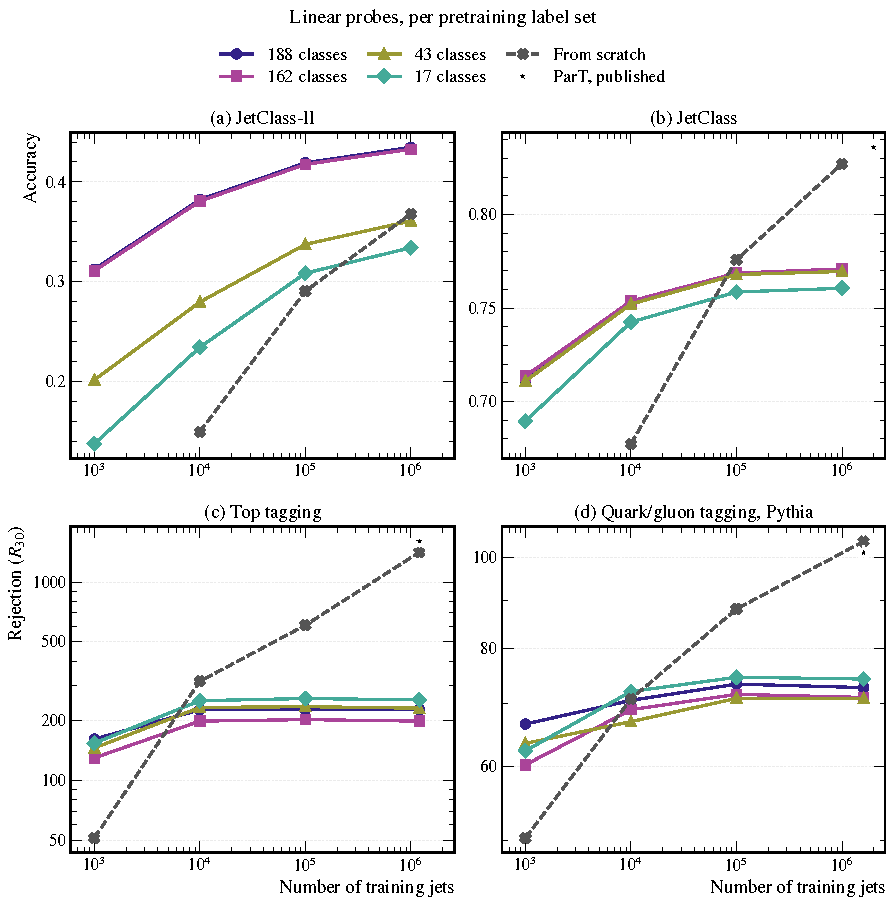
\includegraphics[height=18.5cm]{../../figures/round4/A10.pdf}
\caption{With linear probes, 43 and 17 classes are less accurate on JetClass-II than 188 classes at every training-set size. The upper panels show accuracy on class-balanced JetClass-II and JetClass and $R_{30}$, the inverse background efficiency at 30\% signal efficiency, on top and quark/gluon tagging, Pythia and Herwig, and the lower panels the area under the ROC curve (AUC), averaged over the classes on JetClass-II and JetClass, against training-set size. Error bars are $\pm$1 standard deviation over the runs of figure 1, with points offset by at most 10\% in size. Open stars mark the published Particle Transformer, trained from scratch on 2, 1.2 and 1.6 million jets, with its published standard deviation on $R_{30}$, above every probe. The random network, far below every pretrained network, and every value are in tables A11 and 1.}\label{fig:A10}
\end{figure}
\FloatBarrier
% tables/mlst_probes_n.tex
\providecommand{\TableContinued}[2]{\label{#2}\ifnum\getpagerefnumber{#2}>\getpagerefnumber{#1}\relax\makebox[\linewidth][l]{\textit{Table~\ref{#1} (continued)}}\par\smallskip\fi}
\begin{center}
\setlength{\tabcolsep}{4pt}
\begin{minipage}{\linewidth}\centering
\captionof{table}{Linear probes of table~\ref{tab:summary} at the smaller training sets in the header, in accuracy on class-balanced JetClass-II and JetClass and in $R_{30}$, the inverse background efficiency at 30\% signal efficiency, on top and quark/gluon tagging, Pythia and Herwig. Training jets are counted in total, and the missing inputs are set as in table~\ref{tab:probes}. The 17-class partitions are in the supplementary material. Values are the mean $\pm$ standard deviation over \MlstNRunsWord{} runs, \MlstMassNRunsWord{} per mass network. Bold marks the best value in their column under their italic heading and those within three standard deviations (run spreads and any stored test-jet bootstrap). The random network is a reference, never bold.}
\label{tab:probesn}
\par\medskip
\begin{tabular*}{\linewidth}{@{\extracolsep{\fill}}lccc@{}}
\toprule
 & \multicolumn{3}{c}{training jets} \\
\cmidrule(lr){2-4}
 & 1{,}000 & 10{,}000 & 100{,}000 \\
\midrule
\multicolumn{4}{@{}l}{\textit{linear probe on the frozen features, JetClass-II, accuracy}} \\
\Kfull{} classes & {\fontseries{b}\selectfont 0.3125\,$\pm$\,0.0032} & {\fontseries{b}\selectfont 0.3822\,$\pm$\,0.0006} & {\fontseries{b}\selectfont 0.4191\,$\pm$\,0.0005} \\
\Kres{} classes & {\fontseries{b}\selectfont 0.3109\,$\pm$\,0.0023} & {\fontseries{b}\selectfont 0.3807\,$\pm$\,0.0012} & {\fontseries{b}\selectfont 0.4176\,$\pm$\,0.0009} \\
\Kres{} classes + mass & {\fontseries{b}\selectfont 0.3033\,$\pm$\,0.0006} & 0.3745\,$\pm$\,0.0024 & 0.4126\,$\pm$\,0.0017 \\
\Kmid{} classes & 0.2016\,$\pm$\,0.0014 & 0.280\,$\pm$\,0.004 & 0.337\,$\pm$\,0.005 \\
\Kcoarse{} classes & 0.1376\,$\pm$\,0.0028 & 0.234\,$\pm$\,0.004 & 0.309\,$\pm$\,0.007 \\
\Kcoarse{} classes + mass & 0.135\,$\pm$\,0.008 & 0.237\,$\pm$\,0.024 & 0.304\,$\pm$\,0.027 \\
random network & 0.0200\,$\pm$\,0.0017 & 0.0418\,$\pm$\,0.0019 & 0.0633\,$\pm$\,0.0013 \\
\midrule
\multicolumn{4}{@{}l}{\textit{linear probe on the frozen features, JetClass, accuracy}} \\
\Kfull{} classes & {\fontseries{b}\selectfont 0.711\,$\pm$\,0.006} & {\fontseries{b}\selectfont 0.7529\,$\pm$\,0.0008} & {\fontseries{b}\selectfont 0.7686\,$\pm$\,0.0022} \\
\Kres{} classes & {\fontseries{b}\selectfont 0.714\,$\pm$\,0.008} & {\fontseries{b}\selectfont 0.7537\,$\pm$\,0.0018} & {\fontseries{b}\selectfont 0.76866\,$\pm$\,0.00021} \\
\Kres{} classes + mass & {\fontseries{b}\selectfont 0.7088\,$\pm$\,0.0007} & {\fontseries{b}\selectfont 0.7559\,$\pm$\,0.0022} & {\fontseries{b}\selectfont 0.7718\,$\pm$\,0.0033} \\
\Kmid{} classes & {\fontseries{b}\selectfont 0.7109\,$\pm$\,0.0005} & {\fontseries{b}\selectfont 0.7521\,$\pm$\,0.0004} & {\fontseries{b}\selectfont 0.7679\,$\pm$\,0.0012} \\
\Kcoarse{} classes & {\fontseries{b}\selectfont 0.689\,$\pm$\,0.006} & 0.742\,$\pm$\,0.004 & 0.7586\,$\pm$\,0.0026 \\
\Kcoarse{} classes + mass & {\fontseries{b}\selectfont 0.691\,$\pm$\,0.006} & 0.7436\,$\pm$\,0.0015 & 0.7601\,$\pm$\,0.0008 \\
random network & 0.306\,$\pm$\,0.006 & 0.3854\,$\pm$\,0.0016 & 0.4049\,$\pm$\,0.0016 \\
\bottomrule
\end{tabular*}
\end{minipage}
\par\bigskip
\begin{minipage}{\linewidth}\centering
\TableContinued{tab:probesn}{tab:probesn:2}
\begin{tabular*}{\linewidth}{@{\extracolsep{\fill}}lccc@{}}
\toprule
 & \multicolumn{3}{c}{training jets} \\
\cmidrule(lr){2-4}
 & 1{,}000 & 10{,}000 & 100{,}000 \\
\midrule
\multicolumn{4}{@{}l}{\textit{linear probe on the frozen features, top tagging, $R_{30}$}} \\
\Kfull{} classes & {\fontseries{b}\selectfont 162\,$\pm$\,9} & {\fontseries{b}\selectfont 227\,$\pm$\,18} & {\fontseries{b}\selectfont 228\,$\pm$\,23} \\
\Kres{} classes & 130\,$\pm$\,8 & {\fontseries{b}\selectfont 199\,$\pm$\,21} & {\fontseries{b}\selectfont 203\,$\pm$\,26} \\
\Kres{} classes + mass & {\fontseries{b}\selectfont 193\,$\pm$\,9} & {\fontseries{b}\selectfont 280\,$\pm$\,40} & {\fontseries{b}\selectfont 289\,$\pm$\,33} \\
\Kmid{} classes & {\fontseries{b}\selectfont 146\,$\pm$\,32} & {\fontseries{b}\selectfont 233\,$\pm$\,18} & {\fontseries{b}\selectfont 236\,$\pm$\,10} \\
\Kcoarse{} classes & 154\,$\pm$\,5 & {\fontseries{b}\selectfont 252\,$\pm$\,19} & {\fontseries{b}\selectfont 259\,$\pm$\,20} \\
\Kcoarse{} classes + mass & {\fontseries{b}\selectfont 192.0\,$\pm$\,1.4} & {\fontseries{b}\selectfont 310\,$\pm$\,40} & {\fontseries{b}\selectfont 340\,$\pm$\,50} \\
random network & 43.1\,$\pm$\,1.1 & 55.3\,$\pm$\,3.1 & 57.5\,$\pm$\,3.0 \\
\midrule
\multicolumn{4}{@{}l}{\textit{linear probe on the frozen features, quark/gluon tagging, Pythia jets, $R_{30}$}} \\
\Kfull{} classes & {\fontseries{b}\selectfont 66.5\,$\pm$\,1.7} & {\fontseries{b}\selectfont 70.5\,$\pm$\,1.8} & {\fontseries{b}\selectfont 73.4\,$\pm$\,2.0} \\
\Kres{} classes & {\fontseries{b}\selectfont 60.2\,$\pm$\,1.6} & {\fontseries{b}\selectfont 68.9\,$\pm$\,0.9} & {\fontseries{b}\selectfont 71.5\,$\pm$\,0.8} \\
\Kres{} classes + mass & {\fontseries{b}\selectfont 64\,$\pm$\,5} & {\fontseries{b}\selectfont 68.2\,$\pm$\,2.7} & {\fontseries{b}\selectfont 73.1\,$\pm$\,1.7} \\
\Kmid{} classes & {\fontseries{b}\selectfont 63.4\,$\pm$\,2.7} & {\fontseries{b}\selectfont 66.9\,$\pm$\,0.6} & {\fontseries{b}\selectfont 70.9\,$\pm$\,1.4} \\
\Kcoarse{} classes & {\fontseries{b}\selectfont 62\,$\pm$\,4} & {\fontseries{b}\selectfont 72.0\,$\pm$\,1.8} & {\fontseries{b}\selectfont 74.6\,$\pm$\,1.6} \\
\Kcoarse{} classes + mass & {\fontseries{b}\selectfont 64\,$\pm$\,4} & {\fontseries{b}\selectfont 66.9\,$\pm$\,3.4} & {\fontseries{b}\selectfont 69.9\,$\pm$\,1.4} \\
random network & 43.0\,$\pm$\,2.5 & 55.6\,$\pm$\,1.2 & 56.7\,$\pm$\,0.5 \\
\midrule
\multicolumn{4}{@{}l}{\textit{linear probe on the frozen features, quark/gluon tagging, Herwig jets, $R_{30}$}} \\
\Kfull{} classes & {\fontseries{b}\selectfont 32.99\,$\pm$\,0.13} & {\fontseries{b}\selectfont 34.5\,$\pm$\,1.2} & {\fontseries{b}\selectfont 34.5\,$\pm$\,2.4} \\
\Kres{} classes & {\fontseries{b}\selectfont 31.3\,$\pm$\,2.5} & {\fontseries{b}\selectfont 35.0\,$\pm$\,2.2} & {\fontseries{b}\selectfont 35.8\,$\pm$\,1.9} \\
\Kres{} classes + mass & {\fontseries{b}\selectfont 33.2\,$\pm$\,2.2} & {\fontseries{b}\selectfont 33.92\,$\pm$\,0.10} & {\fontseries{b}\selectfont 35.0\,$\pm$\,0.7} \\
\Kmid{} classes & {\fontseries{b}\selectfont 31.8\,$\pm$\,0.8} & {\fontseries{b}\selectfont 32.4\,$\pm$\,1.7} & {\fontseries{b}\selectfont 34.6\,$\pm$\,1.8} \\
\Kcoarse{} classes & {\fontseries{b}\selectfont 31.0\,$\pm$\,2.8} & {\fontseries{b}\selectfont 34.5\,$\pm$\,1.1} & {\fontseries{b}\selectfont 35.3\,$\pm$\,0.9} \\
\Kcoarse{} classes + mass & {\fontseries{b}\selectfont 33.1\,$\pm$\,1.0} & {\fontseries{b}\selectfont 33.70\,$\pm$\,0.35} & {\fontseries{b}\selectfont 35.0\,$\pm$\,0.8} \\
random network & 25.2\,$\pm$\,1.0 & 30.8\,$\pm$\,0.4 & 31.9\,$\pm$\,1.3 \\
\bottomrule
\end{tabular*}
\end{minipage}
\end{center}
\FloatBarrier
% tables/mlst_ft.tex
\providecommand{\TableContinued}[2]{\label{#2}\ifnum\getpagerefnumber{#2}>\getpagerefnumber{#1}\relax\makebox[\linewidth][l]{\textit{Table~\ref{#1} (continued)}}\par\smallskip\fi}
\begin{center}
\setlength{\tabcolsep}{4pt}
\begin{minipage}{\linewidth}\centering
\captionof{table}{The fine-tuned networks of table~\ref{tab:summary} and from scratch at the smaller training sets, in accuracy on class-balanced JetClass-II and JetClass and $R_{30}$, the inverse background efficiency at 30\% signal efficiency, on top and quark/gluon tagging, Pythia and Herwig, with the missing top and quark/gluon inputs at zero. The 17-class partitions are in the supplementary material. Values are the mean $\pm$ standard deviation over \MlstNRunsWord{} runs, \MlstMassNRunsWord{} per mass network. Bold marks the best value in their column under their italic heading and those within three standard deviations (run spreads and any stored test-jet bootstrap). From scratch is a reference, never bold.}
\label{tab:ft}
\par\medskip
\begin{tabular*}{\linewidth}{@{\extracolsep{\fill}}lcc@{}}
\toprule
 & \multicolumn{2}{c}{training jets} \\
\cmidrule(lr){2-3}
 & 10{,}000 & 100{,}000 \\
\midrule
\multicolumn{3}{@{}l}{\textit{fine-tuned, JetClass-II, accuracy}} \\
\midrule
\multicolumn{3}{@{}l}{\textit{fine-tuned, JetClass, accuracy}} \\
\Kfull{} classes & {\fontseries{b}\selectfont 0.801\,$\pm$\,0.007} & {\fontseries{b}\selectfont 0.8292\,$\pm$\,0.0023} \\
\Kres{} classes & {\fontseries{b}\selectfont 0.803\,$\pm$\,0.005} & {\fontseries{b}\selectfont 0.8292\,$\pm$\,0.0021} \\
\Kres{} classes + mass & {\fontseries{b}\selectfont 0.7990\,$\pm$\,0.0030} & {\fontseries{b}\selectfont 0.8270\,$\pm$\,0.0012} \\
\Kmid{} classes & {\fontseries{b}\selectfont 0.8047\,$\pm$\,0.0032} & {\fontseries{b}\selectfont 0.8259\,$\pm$\,0.0023} \\
\Kcoarse{} classes & {\fontseries{b}\selectfont 0.796\,$\pm$\,0.004} & {\fontseries{b}\selectfont 0.8218\,$\pm$\,0.0020} \\
\Kcoarse{} classes + mass & 0.79105\,$\pm$\,0.00013 & {\fontseries{b}\selectfont 0.8216\,$\pm$\,0.0017} \\
from scratch & 0.6850\,$\pm$\,0.0011 & 0.779\,$\pm$\,0.005 \\
\bottomrule
\end{tabular*}
\end{minipage}
\par\bigskip
\begin{minipage}{\linewidth}\centering
\TableContinued{tab:ft}{tab:ft:2}
\begin{tabular*}{\linewidth}{@{\extracolsep{\fill}}lcc@{}}
\toprule
 & \multicolumn{2}{c}{training jets} \\
\cmidrule(lr){2-3}
 & 10{,}000 & 100{,}000 \\
\midrule
\multicolumn{3}{@{}l}{\textit{fine-tuned, top tagging, $R_{30}$}} \\
\Kfull{} classes & {\fontseries{b}\selectfont 540\,$\pm$\,60} & {\fontseries{b}\selectfont 1{,}030\,$\pm$\,130} \\
\Kres{} classes & {\fontseries{b}\selectfont 530\,$\pm$\,40} & {\fontseries{b}\selectfont 960\,$\pm$\,70} \\
\Kres{} classes + mass & {\fontseries{b}\selectfont 470\,$\pm$\,12} & {\fontseries{b}\selectfont 997\,$\pm$\,17} \\
\Kmid{} classes & {\fontseries{b}\selectfont 532\,$\pm$\,9} & {\fontseries{b}\selectfont 950\,$\pm$\,60} \\
\Kcoarse{} classes & {\fontseries{b}\selectfont 450\,$\pm$\,40} & {\fontseries{b}\selectfont 930\,$\pm$\,50} \\
\Kcoarse{} classes + mass & {\fontseries{b}\selectfont 409\,$\pm$\,12} & {\fontseries{b}\selectfont 920\,$\pm$\,40} \\
from scratch & 310\,$\pm$\,80 & 590\,$\pm$\,100 \\
\midrule
\multicolumn{3}{@{}l}{\textit{fine-tuned, quark/gluon tagging, Pythia jets, $R_{30}$}} \\
\Kfull{} classes & {\fontseries{b}\selectfont 79\,$\pm$\,9} & {\fontseries{b}\selectfont 98.4\,$\pm$\,2.6} \\
\Kres{} classes & {\fontseries{b}\selectfont 80.6\,$\pm$\,1.4} & {\fontseries{b}\selectfont 98.3\,$\pm$\,0.6} \\
\Kres{} classes + mass & {\fontseries{b}\selectfont 79\,$\pm$\,5} & {\fontseries{b}\selectfont 94.7\,$\pm$\,2.9} \\
\Kmid{} classes & {\fontseries{b}\selectfont 78\,$\pm$\,5} & {\fontseries{b}\selectfont 97.1\,$\pm$\,2.6} \\
\Kcoarse{} classes & {\fontseries{b}\selectfont 82.9\,$\pm$\,3.0} & {\fontseries{b}\selectfont 98.20\,$\pm$\,0.15} \\
\Kcoarse{} classes + mass & {\fontseries{b}\selectfont 83.6\,$\pm$\,1.9} & {\fontseries{b}\selectfont 96.1\,$\pm$\,2.2} \\
from scratch & 67\,$\pm$\,4 & 90.2\,$\pm$\,1.0 \\
\midrule
\multicolumn{3}{@{}l}{\textit{fine-tuned, quark/gluon tagging, Herwig jets, $R_{30}$}} \\
\Kfull{} classes & {\fontseries{b}\selectfont 30\,$\pm$\,7} & {\fontseries{b}\selectfont 35\,$\pm$\,5} \\
\Kres{} classes & {\fontseries{b}\selectfont 32.7\,$\pm$\,2.3} & {\fontseries{b}\selectfont 37.9\,$\pm$\,2.7} \\
\Kres{} classes + mass & {\fontseries{b}\selectfont 32\,$\pm$\,6} & {\fontseries{b}\selectfont 36\,$\pm$\,7} \\
\Kmid{} classes & {\fontseries{b}\selectfont 33\,$\pm$\,6} & {\fontseries{b}\selectfont 37\,$\pm$\,4} \\
\Kcoarse{} classes & {\fontseries{b}\selectfont 38.2\,$\pm$\,2.1} & {\fontseries{b}\selectfont 37.6\,$\pm$\,2.2} \\
\Kcoarse{} classes + mass & {\fontseries{b}\selectfont 37.0\,$\pm$\,0.4} & {\fontseries{b}\selectfont 34.3\,$\pm$\,1.9} \\
from scratch & 31.2\,$\pm$\,2.4 & 37.6\,$\pm$\,0.6 \\
\bottomrule
\end{tabular*}
\end{minipage}
\end{center}
\FloatBarrier
\clearpage
\paragraph*{ROC curves}\mbox{}

\nopagebreak
\begin{figure}[H]
\centering
\includegraphics[width=\linewidth]{../../figures/round4/ROC-main.pdf}
\caption{Background rejection against signal efficiency with linear probes on frozen features, the mean over runs. (a)-(i) Every JetClass signal class against QCD jets, as the Particle Transformer reports JetClass; (j) top and (k) quark/gluon tagging (Pythia). Every panel shows the label sets and mass networks; only 188 classes carries a band of the standard deviation over runs. Panels (e) and (i), the leptonic decays, show signal efficiencies from 0.95. Curves end where fewer than 20 background jets remain. Figure A8 shows the fine-tuned networks, and tables A13 and 1 the values.}\label{fig:ROC-main}
\end{figure}
\FloatBarrier
\clearpage
\begin{figure}[H]
\centering
\includegraphics[width=\linewidth]{../../figures/round4/ROC-main-ft.pdf}
\caption{Background rejection against signal efficiency after fine-tuning, the mean over runs. (a)-(i) Every JetClass signal class against QCD jets, fine-tuned on one million JetClass jets, as the Particle Transformer reports JetClass; (j) top and (k) quark/gluon tagging (Pythia), fine-tuned on the full sets. Every panel shows the label sets and mass networks, with training from scratch (grey); only 188 classes and from scratch carry bands of the standard deviation over runs. Panels (e) and (i), the leptonic decays, show signal efficiencies from 0.95. Curves end where fewer than 20 background jets remain. Values are in tables A6, A14 and 1.}\label{fig:ROC-main-ft}
\end{figure}
\FloatBarrier
% tables/mlst_probes.tex
\begin{landscape}
{
\setlength{\LTleft}{0pt}\setlength{\LTright}{0pt}\setlength{\LTcapwidth}{\linewidth}\makeatletter\def\LT@makecaption#1#2#3{\LT@mcol\LT@cols c{\hbox to\z@{\hss\parbox[t]\LTcapwidth{\normalsize #1{#2. }#3\par\vskip\belowcaptionskip}\hss}}}\makeatother
\setlength{\tabcolsep}{6pt}
\begin{center}
\begin{minipage}{\linewidth}\centering
\setlength{\abovecaptionskip}{0pt}
\captionof{table}{Linear probes of table~\ref{tab:summary} on top and quark/gluon tagging, Pythia and Herwig, in accuracy and $R_{50}$, the inverse background efficiency at 50\% signal efficiency. The missing inputs (table~\ref{tab:inputs}) are \LpSubstitutionTop{} for top and \LpSubstitutionQg{} for quark/gluon, chosen on validation, and zero for the released Sophon checkpoint. Beyond three standard deviations of the runs and the test jets, \Kcoarse{} classes + mass is more accurate than \Kfull{} classes on top tagging, with a higher $R_{50}$; no other label set or mass network differs from \Kfull{} classes in these metrics, nor a mass network from its own label set. The 17-class partitions are in the supplementary material. Values are the mean $\pm$ standard deviation over \MlstNRunsWord{} runs, \MlstMassNRunsWord{} per mass network. Bold marks the best value in their column and those within three standard deviations (run spreads and any stored test-jet bootstrap). References (random network, kinematic-inputs network, released Sophon checkpoint) are never bold. $^{\S}$~marks a value from a single run. $^{\P}$~marks a run spread below the last digit shown.}
\label{tab:probes}
\par\medskip
\begin{tabular*}{\linewidth}{@{\extracolsep{\fill}}lcccccc@{}}
\toprule
 & \multicolumn{2}{c}{top tagging} & \multicolumn{2}{c}{quark/gluon, Pythia jets} & \multicolumn{2}{c}{quark/gluon, Herwig jets} \\
\cmidrule(lr){2-3}\cmidrule(lr){4-5}\cmidrule(lr){6-7}
 & accuracy & $R_{50}$ & accuracy & $R_{50}$ & accuracy & $R_{50}$ \\
\midrule
\multicolumn{7}{@{}l}{\textit{linear probe on the frozen features}} \\
\Kfull{} classes & 0.9112\,$\pm$\,0.0015 & 87\,$\pm$\,4 & {\fontseries{b}\selectfont 0.8076\,$\pm$\,0.0004} & {\fontseries{b}\selectfont 26.17\,$\pm$\,0.34} & {\fontseries{b}\selectfont 0.7229\,$\pm$\,0.0033} & {\fontseries{b}\selectfont 11.81\,$\pm$\,0.10} \\
\Kres{} classes & {\fontseries{b}\selectfont 0.9098\,$\pm$\,0.0031} & 79\,$\pm$\,9 & {\fontseries{b}\selectfont 0.8051\,$\pm$\,0.0015} & {\fontseries{b}\selectfont 25.6\,$\pm$\,0.4} & {\fontseries{b}\selectfont 0.7234\,$\pm$\,0.0022} & {\fontseries{b}\selectfont 11.6\,$\pm$\,0.4} \\
\Kres{} classes + mass & {\fontseries{b}\selectfont 0.9145\,$\pm$\,0.0030} & {\fontseries{b}\selectfont 100\,$\pm$\,4} & {\fontseries{b}\selectfont 0.80740\,$\pm$\,0.00020} & {\fontseries{b}\selectfont 25.61\,$\pm$\,0.11} & {\fontseries{b}\selectfont 0.7223\,$\pm$\,0.0006} & {\fontseries{b}\selectfont 11.83\,$\pm$\,0.17} \\
\Kmid{} classes & 0.9101\,$\pm$\,0.0019 & 87.8\,$\pm$\,3.5 & {\fontseries{b}\selectfont 0.8055\,$\pm$\,0.0009} & {\fontseries{b}\selectfont 25.7\,$\pm$\,0.6} & 0.7206\,$\pm$\,0.0005 & {\fontseries{b}\selectfont 11.52\,$\pm$\,0.23} \\
\Kcoarse{} classes & {\fontseries{b}\selectfont 0.9152\,$\pm$\,0.0010} & {\fontseries{b}\selectfont 97\,$\pm$\,4} & {\fontseries{b}\selectfont 0.8064\,$\pm$\,0.0014} & {\fontseries{b}\selectfont 25.8\,$\pm$\,0.7} & {\fontseries{b}\selectfont 0.7201\,$\pm$\,0.0028} & {\fontseries{b}\selectfont 11.50\,$\pm$\,0.16} \\
\Kcoarse{} classes + mass & {\fontseries{b}\selectfont 0.9196\,$\pm$\,0.0015} & {\fontseries{b}\selectfont 118\,$\pm$\,9} & {\fontseries{b}\selectfont 0.8051\,$\pm$\,0.0016} & {\fontseries{b}\selectfont 25.86\,$\pm$\,0.09} & {\fontseries{b}\selectfont 0.7249\,$\pm$\,0.0011} & {\fontseries{b}\selectfont 11.93}$^{\P}$ \\
random network & 0.8867\,$\pm$\,0.0013 & 25.0\,$\pm$\,0.8 & 0.7851\,$\pm$\,0.0018 & 19.40\,$\pm$\,0.29 & 0.7205\,$\pm$\,0.0021 & 10.58\,$\pm$\,0.11 \\
\Kfull{} classes, kinematic inputs only & 0.9163$^{\S}$ & 94$^{\S}$ & -- & -- & -- & -- \\
\midrule
released Sophon checkpoint & 0.9114$^{\S}$ & 77$^{\S}$ & 0.8065$^{\S}$ & 25.3$^{\S}$ & 0.7215$^{\S}$ & 11.69$^{\S}$ \\
\bottomrule
\end{tabular*}
\end{minipage}
\end{center}
}
\end{landscape}
\FloatBarrier
% tables/mlst_labelsets.tex
\begin{landscape}
\begin{center}
\begin{minipage}{\linewidth}\centering
\centering
\setlength{\tabcolsep}{6pt}
\captionof{table}{The fine-tuned networks of table~\ref{tab:summary} and training from scratch on the full top and quark/gluon training sets, in accuracy and $R_{50}$, the inverse background efficiency at 50\% signal efficiency, with top jets and quarks as signal, scored on Pythia and Herwig jets (top tagging Pythia only). The rows for \Kfull{} classes and from scratch repeat those of table~\ref{tab:published}. Beyond three standard deviations of the runs and the test jets, no pretrained network fine-tuned here differs from \Kfull{} classes in these metrics, nor a mass network from its own label set. The 17-class partitions are in the supplementary material. Values are the mean $\pm$ standard deviation over \MlstNRunsWord{} runs, \MlstMassNRunsWord{} per mass network. Bold marks the best value in their column and those within three standard deviations (run spreads and any stored test-jet bootstrap). From scratch is a reference, never bold. $^{\P}$~marks a run spread below the last digit shown.}
\label{tab:labelsets}
\begin{tabular*}{\linewidth}{@{\extracolsep{\fill}}lcccccc@{}}
\toprule
 & \multicolumn{2}{c}{top tagging} & \multicolumn{2}{c}{quark/gluon, Pythia jets} & \multicolumn{2}{c}{quark/gluon, Herwig jets} \\
\cmidrule(lr){2-3}\cmidrule(lr){4-5}\cmidrule(lr){6-7}
 & accuracy & $R_{50}$ & accuracy & $R_{50}$ & accuracy & $R_{50}$ \\
\midrule
\multicolumn{7}{@{}l}{\textit{fine-tuned}} \\
\Kfull{} classes & {\fontseries{b}\selectfont 0.94001\,$\pm$\,0.00023} & {\fontseries{b}\selectfont 461\,$\pm$\,4} & {\fontseries{b}\selectfont 0.84329\,$\pm$\,0.00020} & {\fontseries{b}\selectfont 42.56\,$\pm$\,0.10} & {\fontseries{b}\selectfont 0.712\,$\pm$\,0.005} & {\fontseries{b}\selectfont 12.3\,$\pm$\,0.4} \\
\Kres{} classes & {\fontseries{b}\selectfont 0.94013\,$\pm$\,0.00018} & {\fontseries{b}\selectfont 443\,$\pm$\,17} & {\fontseries{b}\selectfont 0.84318}$^{\P}$ & {\fontseries{b}\selectfont 42.39\,$\pm$\,0.22} & {\fontseries{b}\selectfont 0.7100\,$\pm$\,0.0017} & {\fontseries{b}\selectfont 12.33\,$\pm$\,0.28} \\
\Kres{} classes + mass & {\fontseries{b}\selectfont 0.94039\,$\pm$\,0.00026} & {\fontseries{b}\selectfont 428\,$\pm$\,12} & {\fontseries{b}\selectfont 0.84264\,$\pm$\,0.00014} & {\fontseries{b}\selectfont 42.34\,$\pm$\,0.18} & {\fontseries{b}\selectfont 0.715\,$\pm$\,0.004} & {\fontseries{b}\selectfont 12.6\,$\pm$\,0.6} \\
\Kmid{} classes & {\fontseries{b}\selectfont 0.9402\,$\pm$\,0.0004} & {\fontseries{b}\selectfont 450\,$\pm$\,13} & {\fontseries{b}\selectfont 0.8430\,$\pm$\,0.0005} & {\fontseries{b}\selectfont 42.2\,$\pm$\,0.8} & {\fontseries{b}\selectfont 0.713\,$\pm$\,0.006} & {\fontseries{b}\selectfont 12.5\,$\pm$\,0.6} \\
\Kcoarse{} classes & {\fontseries{b}\selectfont 0.93981\,$\pm$\,0.00014} & {\fontseries{b}\selectfont 429\,$\pm$\,10} & {\fontseries{b}\selectfont 0.84265\,$\pm$\,0.00035} & {\fontseries{b}\selectfont 41.97\,$\pm$\,0.25} & {\fontseries{b}\selectfont 0.7175\,$\pm$\,0.0033} & {\fontseries{b}\selectfont 12.79\,$\pm$\,0.20} \\
\Kcoarse{} classes + mass & {\fontseries{b}\selectfont 0.93983\,$\pm$\,0.00015} & 428\,$\pm$\,10 & 0.84245\,$\pm$\,0.00001 & 41.58\,$\pm$\,0.27 & {\fontseries{b}\selectfont 0.713\,$\pm$\,0.004} & {\fontseries{b}\selectfont 12.3\,$\pm$\,0.4} \\
from scratch & 0.93875\,$\pm$\,0.00016 & 358\,$\pm$\,11 & 0.8397\,$\pm$\,0.0007 & 41.47\,$\pm$\,0.29 & 0.7153\,$\pm$\,0.0024 & 12.18\,$\pm$\,0.11 \\
\bottomrule
\end{tabular*}
\end{minipage}
\end{center}
\end{landscape}
\FloatBarrier
\clearpage
\paragraph*{Jet $p_{\mathrm{T}}$}\mbox{}

\nopagebreak
\begin{figure}[H]
\centering
\fbox{\parbox[c][3cm]{0.6\linewidth}{\centering pending}}
\caption{Pending (preview: waits for the rerun results). Per jet-pT bin, 43 and 17 classes trail 188 on JetClass-II probes; fine-tuned, 17 classes trail in every JetClass-II bin and the two lowest JetClass bins, and as a linear probe in the highest JetClass bin.}\label{fig:PT}
\end{figure}
\FloatBarrier
\clearpage
\paragraph*{Mass}\mbox{}

\nopagebreak
\begin{figure}[H]
\centering
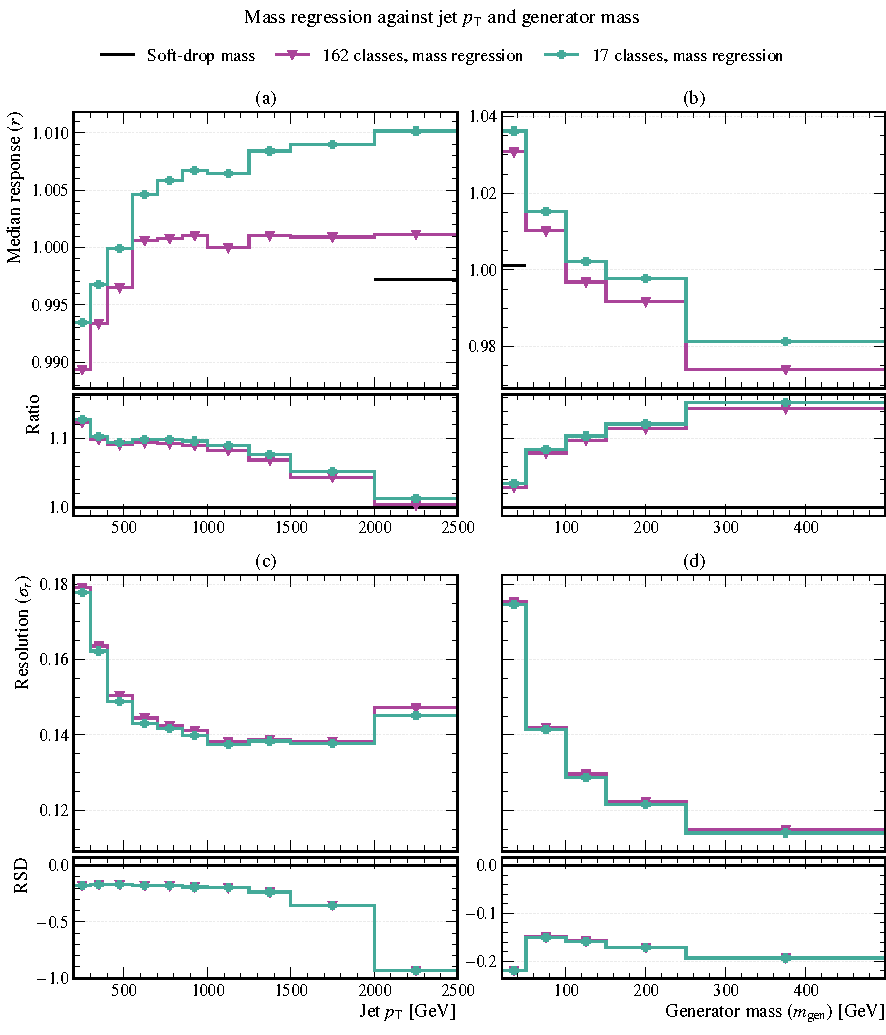
\includegraphics[width=\linewidth]{../../figures/round4/F9b.pdf}
\caption{Each network with an added mass regression (+ mass) resolves the jet mass better than the soft-drop mass in every bin of jet $p_{\mathrm{T}}$ and generator mass, and is less biased in 13 of the 15 bins but more biased in the lowest generator-mass bin, 20 to 50 GeV. Panels (a) and (b) show the median of $r = m/m_{\mathrm{gen}}$, estimated over generator-level soft-drop mass, with its distance from one below, and (c) and (d) the resolution, half the central 68\% range of $r$ over its median, on a logarithmic axis, with the ratio to the soft-drop value below on a linear one. Lines are means over two pretraining runs, flat across each bin, and bands of $\pm$1 standard deviation combine the spread over runs with the bootstrap over test jets. Values are in table 3.}\label{fig:F9b}
\end{figure}
\FloatBarrier
\clearpage
\begin{figure}[H]
\centering
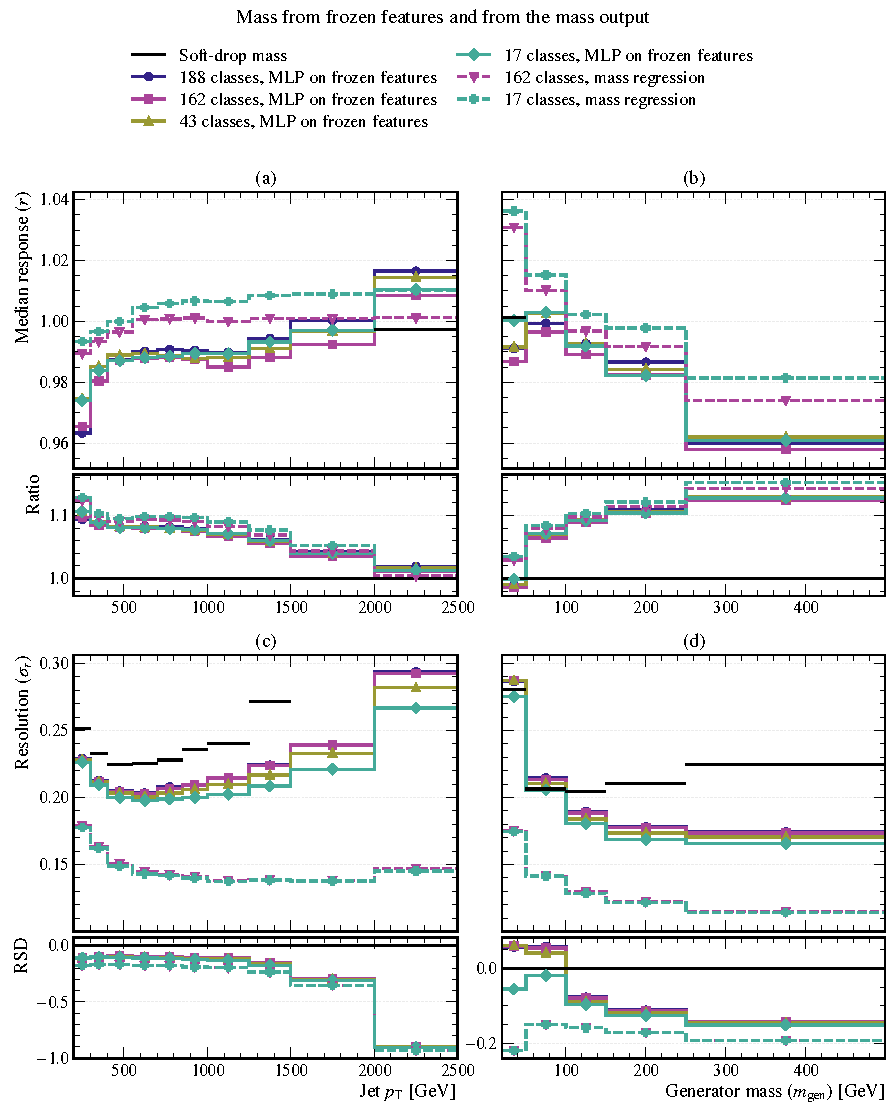
\includegraphics[width=\linewidth]{../../figures/round4/A17-probe.pdf}
\caption{On frozen features, a multilayer-perceptron probe resolves the jet mass better on the networks with an added mass regression (+ mass) than on the same label sets without it. The panels have the form of figure A10, for a probe trained to regress the jet mass from the frozen features of each label set, mass network and the random network (dashed), with the soft-drop mass in black. The probe regresses the mass on frozen features alone, centred on one training median, with no generator-level class information. Lines are means over three pretraining runs, two for + mass, or three random initializations, flat across each bin; the bands, for 188 classes, the random network and the soft-drop mass only, are $\pm$1 standard deviation combining the spread over runs with the bootstrap over test jets. Values, and the other standard deviations, are in table 3.}\label{fig:A17-probe}
\end{figure}
\FloatBarrier
% tables/mlst_masseffect.tex
\begin{landscape}
{
\setlength{\LTleft}{0pt}\setlength{\LTright}{0pt}\setlength{\LTcapwidth}{\linewidth}\makeatletter\def\LT@makecaption#1#2#3{\LT@mcol\LT@cols c{\hbox to\z@{\hss\parbox[t]\LTcapwidth{\normalsize #1{#2. }#3\par\vskip\belowcaptionskip}\hss}}}\makeatother
\setlength{\tabcolsep}{6pt}
\begin{center}
\begin{minipage}{\linewidth}\centering
\setlength{\abovecaptionskip}{0pt}
\captionof{table}{The networks pretrained with 162 and 17 classes, without and with an added mass output, on every task, metric and read-out (rows). Definitions, training sets and inputs are those of tables~\ref{tab:summary}, \ref{tab:mass}, \ref{tab:xbx} and~\ref{tab:sculpt}, the fine-tuned sculpting rows using the networks fine-tuned on JetClass-II. A dash marks a read-out a network lacks, and repeated values are rounded per row. Values are the mean $\pm$ standard deviation over \MlstNRunsWord{} runs, \MlstMassNRunsWord{} per mass network. The best resolution and distance are the lowest, the best median response the closest to one (distances from one compared), and every other value the highest. Bold marks the best value in their row and those within three standard deviations (run spreads and any stored test-jet bootstrap).}
\label{tab:masseffect}
\par\medskip
\begin{tabular*}{\linewidth}{@{\extracolsep{\fill}}lcccc@{}}
\toprule
 & \Kres{} classes & \Kres{} classes + mass & \Kcoarse{} classes & \Kcoarse{} classes + mass \\
 & 3 runs & 2 runs & 3 runs & 2 runs \\
\midrule
\multicolumn{5}{@{}l}{jet mass on JetClass-II, all jets} \\
resolution, mass output of the pretraining head & -- & {\fontseries{b}\selectfont 0.1467\,$\pm$\,0.0006} & -- & {\fontseries{b}\selectfont 0.1455\,$\pm$\,0.0008} \\
median response, mass output of the pretraining head & -- & {\fontseries{b}\selectfont 0.999\,$\pm$\,0.005} & -- & {\fontseries{b}\selectfont 1.00523\,$\pm$\,0.00019} \\
resolution, multilayer-perceptron probe & 0.2173\,$\pm$\,0.0016 & 0.15726\,$\pm$\,0.00003 & 0.2082\,$\pm$\,0.0023 & {\fontseries{b}\selectfont 0.15584\,$\pm$\,0.00023} \\
median response, multilayer-perceptron probe & {\fontseries{b}\selectfont 0.992\,$\pm$\,0.004} & {\fontseries{b}\selectfont 1.0085\,$\pm$\,0.0024} & {\fontseries{b}\selectfont 0.9929\,$\pm$\,0.0033} & {\fontseries{b}\selectfont 1.008\,$\pm$\,0.006} \\
resolution, ridge probe & 0.315\,$\pm$\,0.009 & {\fontseries{b}\selectfont 0.1885\,$\pm$\,0.0022} & 0.292\,$\pm$\,0.012 & {\fontseries{b}\selectfont 0.1814\,$\pm$\,0.0010} \\
median response, ridge probe & 0.9655\,$\pm$\,0.0007 & {\fontseries{b}\selectfont 1.00055\,$\pm$\,0.00001} & 0.973\,$\pm$\,0.005 & 1.0031\,$\pm$\,0.0005 \\
\midrule
\multicolumn{5}{@{}l}{JetClass-II} \\
accuracy, linear probe & {\fontseries{b}\selectfont 0.4328\,$\pm$\,0.0008} & {\fontseries{b}\selectfont 0.4288\,$\pm$\,0.0024} & 0.334\,$\pm$\,0.007 & 0.331\,$\pm$\,0.026 \\
AUC, linear probe & {\fontseries{b}\selectfont 0.97963\,$\pm$\,0.00010} & {\fontseries{b}\selectfont 0.97924\,$\pm$\,0.00023} & 0.9691\,$\pm$\,0.0004 & 0.9688\,$\pm$\,0.0013 \\
accuracy, fine-tuned & -- & -- & -- & -- \\
AUC, fine-tuned & -- & -- & -- & -- \\
\bottomrule
\end{tabular*}
\end{minipage}
\end{center}
\newpage
\begin{center}
\begin{minipage}{\linewidth}\centering
\makebox[\linewidth][l]{\textit{Table~\ref{tab:masseffect} (continued)}}
\par\smallskip
\begin{tabular*}{\linewidth}{@{\extracolsep{\fill}}lcccc@{}}
\toprule
 & \Kres{} classes & \Kres{} classes + mass & \Kcoarse{} classes & \Kcoarse{} classes + mass \\
 & 3 runs & 2 runs & 3 runs & 2 runs \\
\midrule
\multicolumn{5}{@{}l}{JetClass} \\
accuracy, linear probe & {\fontseries{b}\selectfont 0.7709\,$\pm$\,0.0005} & {\fontseries{b}\selectfont 0.7739\,$\pm$\,0.0030} & 0.7606\,$\pm$\,0.0027 & 0.7618\,$\pm$\,0.0009 \\
AUC, linear probe & {\fontseries{b}\selectfont 0.96832\,$\pm$\,0.00016} & {\fontseries{b}\selectfont 0.9690\,$\pm$\,0.0009} & 0.9650\,$\pm$\,0.0008 & 0.96532\,$\pm$\,0.00026 \\
accuracy, multilayer-perceptron probe & {\fontseries{b}\selectfont 0.8123\,$\pm$\,0.0008} & {\fontseries{b}\selectfont 0.8166\,$\pm$\,0.0021} & 0.8060\,$\pm$\,0.0026 & {\fontseries{b}\selectfont 0.81050\,$\pm$\,0.00017} \\
AUC, multilayer-perceptron probe & {\fontseries{b}\selectfont 0.97857\,$\pm$\,0.00018} & {\fontseries{b}\selectfont 0.97964\,$\pm$\,0.00032} & 0.9776\,$\pm$\,0.0005 & {\fontseries{b}\selectfont 0.97863\,$\pm$\,0.00012} \\
accuracy, fine-tuned & -- & -- & -- & -- \\
AUC, fine-tuned & -- & -- & -- & -- \\
\midrule
\multicolumn{5}{@{}l}{top tagging} \\
$R_{30}$, linear probe & {\fontseries{b}\selectfont 199\,$\pm$\,25} & {\fontseries{b}\selectfont 283\,$\pm$\,33} & {\fontseries{b}\selectfont 255\,$\pm$\,17} & {\fontseries{b}\selectfont 340\,$\pm$\,50} \\
AUC, linear probe & 0.9671\,$\pm$\,0.0020 & {\fontseries{b}\selectfont 0.9709\,$\pm$\,0.0009} & {\fontseries{b}\selectfont 0.9710\,$\pm$\,0.0006} & {\fontseries{b}\selectfont 0.9741\,$\pm$\,0.0010} \\
$R_{30}$, multilayer-perceptron probe & {\fontseries{b}\selectfont 280\,$\pm$\,90} & {\fontseries{b}\selectfont 350\,$\pm$\,40} & {\fontseries{b}\selectfont 224\,$\pm$\,24} & {\fontseries{b}\selectfont 310\,$\pm$\,70} \\
$R_{30}$, fine-tuned & {\fontseries{b}\selectfont 1{,}790\,$\pm$\,60} & {\fontseries{b}\selectfont 1{,}770\,$\pm$\,250} & {\fontseries{b}\selectfont 1{,}740\,$\pm$\,140} & {\fontseries{b}\selectfont 1{,}660\,$\pm$\,40} \\
AUC, fine-tuned & {\fontseries{b}\selectfont 0.98610\,$\pm$\,0.00008} & {\fontseries{b}\selectfont 0.98603\,$\pm$\,0.00003} & {\fontseries{b}\selectfont 0.98590\,$\pm$\,0.00006} & {\fontseries{b}\selectfont 0.98583\,$\pm$\,0.00007} \\
\midrule
\multicolumn{5}{@{}l}{quark/gluon tagging, Pythia jets} \\
$R_{30}$, linear probe & {\fontseries{b}\selectfont 70.97\,$\pm$\,0.28} & {\fontseries{b}\selectfont 72.3\,$\pm$\,2.3} & {\fontseries{b}\selectfont 74.3\,$\pm$\,2.0} & {\fontseries{b}\selectfont 70.2\,$\pm$\,3.0} \\
AUC, linear probe & {\fontseries{b}\selectfont 0.8818\,$\pm$\,0.0018} & {\fontseries{b}\selectfont 0.8834\,$\pm$\,0.0005} & {\fontseries{b}\selectfont 0.8821\,$\pm$\,0.0015} & 0.8801\,$\pm$\,0.0006 \\
$R_{30}$, fine-tuned & {\fontseries{b}\selectfont 108.0\,$\pm$\,1.4} & {\fontseries{b}\selectfont 106.78\,$\pm$\,0.24} & {\fontseries{b}\selectfont 106.5\,$\pm$\,0.8} & {\fontseries{b}\selectfont 105.3\,$\pm$\,0.5} \\
AUC, fine-tuned & {\fontseries{b}\selectfont 0.91478\,$\pm$\,0.00008} & {\fontseries{b}\selectfont 0.91461\,$\pm$\,0.00011} & 0.91440\,$\pm$\,0.00003 & 0.91409\,$\pm$\,0.00013 \\
\bottomrule
\end{tabular*}
\end{minipage}
\end{center}
\newpage
\begin{center}
\begin{minipage}{\linewidth}\centering
\makebox[\linewidth][l]{\textit{Table~\ref{tab:masseffect} (continued)}}
\par\smallskip
\begin{tabular*}{\linewidth}{@{\extracolsep{\fill}}lcccc@{}}
\toprule
 & \Kres{} classes & \Kres{} classes + mass & \Kcoarse{} classes & \Kcoarse{} classes + mass \\
 & 3 runs & 2 runs & 3 runs & 2 runs \\
\midrule
\multicolumn{5}{@{}l}{quark/gluon tagging, Herwig jets} \\
$R_{30}$, linear probe & {\fontseries{b}\selectfont 35.9\,$\pm$\,1.7} & {\fontseries{b}\selectfont 35.3\,$\pm$\,0.5} & {\fontseries{b}\selectfont 35.5\,$\pm$\,1.0} & {\fontseries{b}\selectfont 35.5\,$\pm$\,1.2} \\
AUC, linear probe & {\fontseries{b}\selectfont 0.8068\,$\pm$\,0.0022} & {\fontseries{b}\selectfont 0.8071\,$\pm$\,0.0010} & {\fontseries{b}\selectfont 0.8053\,$\pm$\,0.0020} & {\fontseries{b}\selectfont 0.80794\,$\pm$\,0.00009} \\
$R_{30}$, fine-tuned & {\fontseries{b}\selectfont 34.6\,$\pm$\,2.0} & {\fontseries{b}\selectfont 36.1\,$\pm$\,2.4} & {\fontseries{b}\selectfont 36.9\,$\pm$\,0.9} & {\fontseries{b}\selectfont 35.3\,$\pm$\,3.4} \\
AUC, fine-tuned & {\fontseries{b}\selectfont 0.8074\,$\pm$\,0.0010} & {\fontseries{b}\selectfont 0.8091\,$\pm$\,0.0025} & {\fontseries{b}\selectfont 0.8103\,$\pm$\,0.0018} & {\fontseries{b}\selectfont 0.8076\,$\pm$\,0.0034} \\
\midrule
\multicolumn{5}{@{}l}{$X\to b\bar b$ against QCD at 1\% QCD efficiency} \\
signal efficiency (\%), classifier & {\fontseries{b}\selectfont 71.69\,$\pm$\,0.27} & {\fontseries{b}\selectfont 71.1\,$\pm$\,0.5} & 65.9\,$\pm$\,1.0 & 66.78\,$\pm$\,0.25 \\
signal efficiency (\%), linear probe & {\fontseries{b}\selectfont 69.7\,$\pm$\,0.4} & {\fontseries{b}\selectfont 70.1\,$\pm$\,1.2} & {\fontseries{b}\selectfont 67.0\,$\pm$\,1.1} & {\fontseries{b}\selectfont 68.3\,$\pm$\,1.8} \\
signal efficiency (\%), direct & {\fontseries{b}\selectfont 69.95\,$\pm$\,0.19} & {\fontseries{b}\selectfont 69.71\,$\pm$\,0.21} & -- & -- \\
\midrule
\multicolumn{5}{@{}l}{$X\to bs$ against QCD at 1\% QCD efficiency} \\
signal efficiency (\%), classifier & {\fontseries{b}\selectfont 68.90\,$\pm$\,0.06} & 68.03\,$\pm$\,0.05 & 59.4\,$\pm$\,1.6 & 59.9\,$\pm$\,1.2 \\
signal efficiency (\%), linear probe & {\fontseries{b}\selectfont 65.4\,$\pm$\,0.9} & {\fontseries{b}\selectfont 64.6\,$\pm$\,0.7} & 58.6\,$\pm$\,2.0 & 59.6\,$\pm$\,1.0 \\
\midrule
\multicolumn{5}{@{}l}{Jensen--Shannon distance of the QCD jet mass} \\
at 10\% QCD efficiency, network output used directly & {\fontseries{b}\selectfont 0.0532\,$\pm$\,0.0009} & {\fontseries{b}\selectfont 0.0443\,$\pm$\,0.0030} & 0.0543\,$\pm$\,0.0010 & {\fontseries{b}\selectfont 0.047\,$\pm$\,0.007} \\
at 1\% QCD efficiency, network output used directly & {\fontseries{b}\selectfont 0.0429\,$\pm$\,0.0029} & {\fontseries{b}\selectfont 0.0433\,$\pm$\,0.0012} & 0.0561\,$\pm$\,0.0017 & {\fontseries{b}\selectfont 0.0428\,$\pm$\,0.0033} \\
at 50\% signal efficiency, network output used directly & {\fontseries{b}\selectfont 0.0554\,$\pm$\,0.0015} & {\fontseries{b}\selectfont 0.0548\,$\pm$\,0.0032} & 0.0668\,$\pm$\,0.0022 & {\fontseries{b}\selectfont 0.051\,$\pm$\,0.004} \\
at 10\% QCD efficiency, fine-tuned & -- & -- & -- & -- \\
at 1\% QCD efficiency, fine-tuned & -- & -- & -- & -- \\
at 50\% signal efficiency, fine-tuned & -- & -- & -- & -- \\
\bottomrule
\end{tabular*}
\end{minipage}
\end{center}
\par\smallskip{\noindent Quark/gluon tagging trains on Pythia jets.}
}
\end{landscape}
\FloatBarrier
% tables/mlst_mass_detail.tex
\begin{landscape}
{
\setlength{\LTleft}{0pt}\setlength{\LTright}{0pt}\setlength{\LTcapwidth}{\linewidth}\makeatletter\def\LT@makecaption#1#2#3{\LT@mcol\LT@cols c{\hbox to\z@{\hss\parbox[t]\LTcapwidth{\normalsize #1{#2. }#3\par\vskip\belowcaptionskip}\hss}}}\makeatother
\addtolength{\belowcaptionskip}{\medskipamount}
\begin{longtable}{@{\extracolsep{\fill}}lccc@{}}
\caption{Jet-mass resolution and median response on JetClass-II in detail, defined as in table~\ref{tab:mass}. In the upper part a cell over all jets is empty where table~\ref{tab:mass} holds it. The lower parts give the bins of jet $p_{\mathrm{T}}$ and generator-level soft-drop mass of figures A10, S41, S42, A11 and S43, the mass output over all, resonant and QCD jets and the two regression probes over all jets, and every bin holds at least \MlstMassMinJets{} jets. The soft-drop mass has no run-to-run spread. A flavor boundary keeps apart decays that differ only in quark flavor. Values are the mean $\pm$ standard deviation over \MlstNRunsWord{} runs, \MlstMassNRunsWord{} per mass network and flavor-boundary partition, and over five random partitions. $^{\P}$~marks a run spread below the last digit shown.}\label{tab:massdetail}\\
\toprule
& \multicolumn{3}{c}{resolution} \\
\cmidrule(lr){2-4}
jets & all & resonant & QCD \\
\midrule
\endfirsthead
\multicolumn{4}{@{}l}{\textit{Table~\ref{tab:massdetail} (continued)}} \\[\smallskipamount]
\toprule
& \multicolumn{3}{c}{resolution} \\
\cmidrule(lr){2-4}
jets & all & resonant & QCD \\
\midrule
\endhead
soft-drop mass &  & 0.2128\,$\pm$\,0.0005 & 1.525\,$\pm$\,0.027 \\
\multicolumn{4}{@{}l}{{\itshape mass output of the pretraining head}} \\*
\Kres{} classes + mass &  & 0.1326\,$\pm$\,0.0008 & 0.2260\,$\pm$\,0.0006 \\
\Kcoarse{} classes + mass &  & 0.1316\,$\pm$\,0.0006 & 0.22394\,$\pm$\,0.00005 \\
\multicolumn{4}{@{}l}{{\itshape multilayer-perceptron probe on the frozen features}} \\*
\Kfull{} classes &  & 0.1979\,$\pm$\,0.0026 & 0.3438\,$\pm$\,0.0015 \\
\Kres{} classes &  & 0.1977\,$\pm$\,0.0014 & 0.338\,$\pm$\,0.004 \\
\Kres{} classes + mass &  & 0.14258\,$\pm$\,0.00002 & 0.2412\,$\pm$\,0.0007 \\
\Kmid{} classes &  & 0.1948\,$\pm$\,0.0029 & 0.334\,$\pm$\,0.008 \\
\Kcoarse{} classes &  & 0.1887\,$\pm$\,0.0025 & 0.322\,$\pm$\,0.005 \\
\Kcoarse{} classes + mass &  & 0.14108\,$\pm$\,0.00030 & 0.2385\,$\pm$\,0.0016 \\
\multicolumn{4}{@{}l}{\textit{17-class partitions}} \\*
\quad no flavor boundary &  & 0.1927\,$\pm$\,0.0016 & 0.330\,$\pm$\,0.008 \\*
\quad $b$-quark boundary &  & 0.1951\,$\pm$\,0.0007 & 0.3304\,$\pm$\,0.0020 \\*
\quad random flavor boundary &  & 0.1980\,$\pm$\,0.0023 & 0.335\,$\pm$\,0.004 \\*
\quad random partitions &  & 0.2073\,$\pm$\,0.0025 & 0.350\,$\pm$\,0.007 \\
random network &  & 0.2208\,$\pm$\,0.0027 & 0.497\,$\pm$\,0.009 \\
\multicolumn{4}{@{}l}{{\itshape ridge regression on the frozen features}} \\*
\Kfull{} classes & 0.320\,$\pm$\,0.004 & 0.2922\,$\pm$\,0.0029 & 0.552\,$\pm$\,0.014 \\
\Kres{} classes & 0.315\,$\pm$\,0.009 & 0.288\,$\pm$\,0.008 & 0.543\,$\pm$\,0.022 \\
\Kres{} classes + mass & 0.1885\,$\pm$\,0.0022 & 0.1760\,$\pm$\,0.0020 & 0.2610\,$\pm$\,0.0015 \\
\Kmid{} classes & 0.303\,$\pm$\,0.016 & 0.280\,$\pm$\,0.013 & 0.48\,$\pm$\,0.06 \\
\Kcoarse{} classes & 0.292\,$\pm$\,0.012 & 0.271\,$\pm$\,0.012 & 0.443\,$\pm$\,0.031 \\
\Kcoarse{} classes + mass & 0.1814\,$\pm$\,0.0010 & 0.1682\,$\pm$\,0.0006 & 0.2538\,$\pm$\,0.0023 \\
\multicolumn{4}{@{}l}{\textit{17-class partitions}} \\*
\quad no flavor boundary & 0.301\,$\pm$\,0.008 & 0.278\,$\pm$\,0.006 & 0.466\,$\pm$\,0.027 \\*
\quad $b$-quark boundary & 0.3061\,$\pm$\,0.0035 & 0.2812\,$\pm$\,0.0010 & 0.496\,$\pm$\,0.026 \\*
\quad random flavor boundary & 0.30922\,$\pm$\,0.00032 & 0.2848\,$\pm$\,0.0015 & 0.4955\,$\pm$\,0.0032 \\*
\quad random partitions & 0.332\,$\pm$\,0.005 & 0.303\,$\pm$\,0.005 & 0.578\,$\pm$\,0.017 \\*
random network & 0.312\,$\pm$\,0.008 & 0.287\,$\pm$\,0.007 & 0.919\,$\pm$\,0.032 \\
\noalign{\nobreak\vskip\aboverulesep\hrule height\heavyrulewidth}
\end{longtable}
\newpage
\addtocounter{table}{-1}
\begin{longtable}{@{\extracolsep{\fill}}lccc@{}}
\multicolumn{4}{@{}l}{\textit{Table~\ref{tab:massdetail} (continued)}} \\[\smallskipamount]
\toprule
& \multicolumn{3}{c}{median response} \\
\cmidrule(lr){2-4}
jets & all & resonant & QCD \\
\midrule
\endfirsthead
\multicolumn{4}{@{}l}{\textit{Table~\ref{tab:massdetail} (continued)}} \\[\smallskipamount]
\toprule
& \multicolumn{3}{c}{median response} \\
\cmidrule(lr){2-4}
jets & all & resonant & QCD \\
\midrule
\endhead
soft-drop mass &  & 0.9291\,$\pm$\,0.0004 & 0.9309\,$\pm$\,0.0012 \\
\multicolumn{4}{@{}l}{{\itshape mass output of the pretraining head}} \\*
\Kres{} classes + mass &  & 1.000\,$\pm$\,0.005 & 0.995\,$\pm$\,0.007 \\
\Kcoarse{} classes + mass &  & 1.00594\,$\pm$\,0.00013 & 1.0007\,$\pm$\,0.0010 \\
\multicolumn{4}{@{}l}{{\itshape multilayer-perceptron probe on the frozen features}} \\*
\Kfull{} classes &  & 0.9939\,$\pm$\,0.0023 & 0.9802\,$\pm$\,0.0034 \\
\Kres{} classes &  & 0.993\,$\pm$\,0.004 & 0.9873\,$\pm$\,0.0012 \\
\Kres{} classes + mass &  & 1.0102\,$\pm$\,0.0031 & 0.9990\,$\pm$\,0.0018 \\
\Kmid{} classes &  & 0.994\,$\pm$\,0.004 & 0.988\,$\pm$\,0.008 \\
\Kcoarse{} classes &  & 0.9940\,$\pm$\,0.0029 & 0.987\,$\pm$\,0.006 \\
\Kcoarse{} classes + mass &  & 1.008\,$\pm$\,0.006 & 1.0023\,$\pm$\,0.0033 \\
\multicolumn{4}{@{}l}{\textit{17-class partitions}} \\*
\quad no flavor boundary &  & 0.99456\,$\pm$\,0.00001 & 0.98866\,$\pm$\,0.00006 \\*
\quad $b$-quark boundary &  & 0.9904\,$\pm$\,0.0016 & 0.9760\,$\pm$\,0.0013 \\*
\quad random flavor boundary &  & 0.9918\,$\pm$\,0.0006 & 0.9805\,$\pm$\,0.0022 \\*
\quad random partitions &  & 0.9939\,$\pm$\,0.0019 & 0.9824\,$\pm$\,0.0030 \\
random network &  & 0.9800\,$\pm$\,0.0018 & 0.9900\,$\pm$\,0.0024 \\
\multicolumn{4}{@{}l}{{\itshape ridge regression on the frozen features}} \\*
\Kfull{} classes & 0.9644\,$\pm$\,0.0014 & 0.9745\,$\pm$\,0.0008 & 0.912\,$\pm$\,0.006 \\
\Kres{} classes & 0.9655\,$\pm$\,0.0007 & 0.9752\,$\pm$\,0.0007 & 0.917\,$\pm$\,0.008 \\
\Kres{} classes + mass & 1.00055\,$\pm$\,0.00001 & 1.00213$^{\P}$ & 0.99259\,$\pm$\,0.00023 \\
\Kmid{} classes & 0.969\,$\pm$\,0.006 & 0.976\,$\pm$\,0.004 & 0.931\,$\pm$\,0.013 \\
\Kcoarse{} classes & 0.973\,$\pm$\,0.005 & 0.979\,$\pm$\,0.004 & 0.946\,$\pm$\,0.010 \\
\Kcoarse{} classes + mass & 1.0031\,$\pm$\,0.0005 & 1.0036\,$\pm$\,0.0011 & 1.0006\,$\pm$\,0.0028 \\
\multicolumn{4}{@{}l}{\textit{17-class partitions}} \\*
\quad no flavor boundary & 0.969\,$\pm$\,0.006 & 0.975\,$\pm$\,0.007 & 0.93979\,$\pm$\,0.00015 \\*
\quad $b$-quark boundary & 0.9676\,$\pm$\,0.0031 & 0.9766\,$\pm$\,0.0025 & 0.921\,$\pm$\,0.009 \\*
\quad random flavor boundary & 0.9672\,$\pm$\,0.0013 & 0.9742\,$\pm$\,0.0020 & 0.9319\,$\pm$\,0.0034 \\*
\quad random partitions & 0.9625\,$\pm$\,0.0009 & 0.9709\,$\pm$\,0.0011 & 0.919\,$\pm$\,0.005 \\*
random network & 0.940\,$\pm$\,0.004 & 0.933\,$\pm$\,0.004 & 0.979\,$\pm$\,0.004 \\
\noalign{\nobreak\vskip\aboverulesep\hrule height\heavyrulewidth}
\end{longtable}
\newpage
\addtocounter{table}{-1}
\begin{longtable}{@{\extracolsep{\fill}}lccc@{}}
\multicolumn{4}{@{}l}{\textit{Table~\ref{tab:massdetail} (continued)}} \\[\smallskipamount]
\toprule
\textit{resolution} & \multicolumn{3}{c}{jet $p_{\mathrm{T}}$ [GeV]} \\
\cmidrule(lr){2-4}
 & 200--300 & 300--400 & 400--550 \\
\midrule
\endfirsthead
\multicolumn{4}{@{}l}{\textit{Table~\ref{tab:massdetail} (continued)}} \\[\smallskipamount]
\toprule
\textit{resolution} & \multicolumn{3}{c}{jet $p_{\mathrm{T}}$ [GeV]} \\
\cmidrule(lr){2-4}
 & 200--300 & 300--400 & 400--550 \\
\midrule
\endhead
soft-drop mass, all jets & 0.2513\,$\pm$\,0.0016 & 0.2328\,$\pm$\,0.0015 & 0.2246\,$\pm$\,0.0013 \\
\multicolumn{4}{@{}l}{\textit{mass output of the pretraining head, all jets}} \\*
\Kres{} classes + mass & 0.1791\,$\pm$\,0.0004 & 0.1636\,$\pm$\,0.0014 & 0.1504\,$\pm$\,0.0018 \\
\Kcoarse{} classes + mass & 0.1779\,$\pm$\,0.0006 & 0.1623\,$\pm$\,0.0007 & 0.1488\,$\pm$\,0.0007 \\
soft-drop mass, resonant jets & 0.2364\,$\pm$\,0.0021 & 0.2233\,$\pm$\,0.0017 & 0.2142\,$\pm$\,0.0015 \\
\multicolumn{4}{@{}l}{\textit{mass output of the pretraining head, resonant jets}} \\*
\Kres{} classes + mass & 0.1701\,$\pm$\,0.0011 & 0.1575\,$\pm$\,0.0019 & 0.1447\,$\pm$\,0.0018 \\
\Kcoarse{} classes + mass & 0.16851\,$\pm$\,0.00020 & 0.1558\,$\pm$\,0.0010 & 0.1428\,$\pm$\,0.0010 \\
soft-drop mass, QCD jets & 0.281\,$\pm$\,0.004 & 0.274\,$\pm$\,0.004 & 0.290\,$\pm$\,0.005 \\
\multicolumn{4}{@{}l}{\textit{mass output of the pretraining head, QCD jets}} \\*
\Kres{} classes + mass & 0.2001\,$\pm$\,0.0011 & 0.1861\,$\pm$\,0.0020 & 0.17775\,$\pm$\,0.00029 \\
\Kcoarse{} classes + mass & 0.1994\,$\pm$\,0.0021 & 0.1854\,$\pm$\,0.0025 & 0.17650\,$\pm$\,0.00022 \\
\multicolumn{4}{@{}l}{\textit{multilayer-perceptron probe on the frozen features, all jets}} \\*
\Kfull{} classes & 0.2283\,$\pm$\,0.0011 & 0.2110\,$\pm$\,0.0012 & 0.2028\,$\pm$\,0.0016 \\
\Kres{} classes & 0.2254\,$\pm$\,0.0020 & 0.2094\,$\pm$\,0.0019 & 0.2020\,$\pm$\,0.0024 \\
\Kres{} classes + mass & 0.1871\,$\pm$\,0.0023 & 0.17317\,$\pm$\,0.00014 & 0.16082\,$\pm$\,0.00004 \\
\Kmid{} classes & 0.227\,$\pm$\,0.004 & 0.2098\,$\pm$\,0.0026 & 0.2020\,$\pm$\,0.0029 \\
\Kcoarse{} classes & 0.2252\,$\pm$\,0.0031 & 0.2069\,$\pm$\,0.0027 & 0.1986\,$\pm$\,0.0028 \\
\Kcoarse{} classes + mass & 0.1854\,$\pm$\,0.0011 & 0.17117\,$\pm$\,0.00009 & 0.1597\,$\pm$\,0.0005 \\
\multicolumn{4}{@{}l}{\textit{17-class partitions}} \\*
\quad no flavor boundary & 0.2257\,$\pm$\,0.0022 & 0.20939\,$\pm$\,0.00019 & 0.2008\,$\pm$\,0.0017 \\*
\quad $b$-quark boundary & 0.2291\,$\pm$\,0.0023 & 0.2129\,$\pm$\,0.0026 & 0.2027\,$\pm$\,0.0011 \\*
\quad random flavor boundary & 0.2317\,$\pm$\,0.0014 & 0.2134\,$\pm$\,0.0007 & 0.2051\,$\pm$\,0.0025 \\*
\quad random partitions & 0.2380\,$\pm$\,0.0032 & 0.2217\,$\pm$\,0.0029 & 0.214\,$\pm$\,0.004 \\*
random network & 0.2264\,$\pm$\,0.0030 & 0.2150\,$\pm$\,0.0018 & 0.2122\,$\pm$\,0.0030 \\
\noalign{\nobreak\vskip\aboverulesep\hrule height\heavyrulewidth}
\end{longtable}
\newpage
\addtocounter{table}{-1}
\begin{longtable}{@{\extracolsep{\fill}}lccc@{}}
\multicolumn{4}{@{}l}{\textit{Table~\ref{tab:massdetail} (continued)}} \\[\smallskipamount]
\toprule
\textit{resolution} & \multicolumn{3}{c}{jet $p_{\mathrm{T}}$ [GeV]} \\
\cmidrule(lr){2-4}
 & 550--700 & 700--850 & 850--1000 \\
\midrule
\endfirsthead
\multicolumn{4}{@{}l}{\textit{Table~\ref{tab:massdetail} (continued)}} \\[\smallskipamount]
\toprule
\textit{resolution} & \multicolumn{3}{c}{jet $p_{\mathrm{T}}$ [GeV]} \\
\cmidrule(lr){2-4}
 & 550--700 & 700--850 & 850--1000 \\
\midrule
\endhead
soft-drop mass, all jets & 0.2258\,$\pm$\,0.0015 & 0.2280\,$\pm$\,0.0013 & 0.2356\,$\pm$\,0.0017 \\
\multicolumn{4}{@{}l}{\textit{mass output of the pretraining head, all jets}} \\*
\Kres{} classes + mass & 0.1445\,$\pm$\,0.0005 & 0.1424\,$\pm$\,0.0016 & 0.1412\,$\pm$\,0.0004 \\
\Kcoarse{} classes + mass & 0.1430\,$\pm$\,0.0014 & 0.1417\,$\pm$\,0.0007 & 0.1399\,$\pm$\,0.0006 \\
soft-drop mass, resonant jets & 0.2147\,$\pm$\,0.0014 & 0.2152\,$\pm$\,0.0017 & 0.2174\,$\pm$\,0.0014 \\
\multicolumn{4}{@{}l}{\textit{mass output of the pretraining head, resonant jets}} \\*
\Kres{} classes + mass & 0.1362\,$\pm$\,0.0009 & 0.1343\,$\pm$\,0.0022 & 0.1309\,$\pm$\,0.0008 \\
\Kcoarse{} classes + mass & 0.1351\,$\pm$\,0.0010 & 0.1336\,$\pm$\,0.0010 & 0.12973\,$\pm$\,0.00016 \\
soft-drop mass, QCD jets & 0.440\,$\pm$\,0.025 & 0.85\,$\pm$\,0.06 & 1.46\,$\pm$\,0.09 \\
\multicolumn{4}{@{}l}{\textit{mass output of the pretraining head, QCD jets}} \\*
\Kres{} classes + mass & 0.1944\,$\pm$\,0.0011 & 0.2020\,$\pm$\,0.0014 & 0.2243\,$\pm$\,0.0020 \\
\Kcoarse{} classes + mass & 0.18969\,$\pm$\,0.00020 & 0.1985\,$\pm$\,0.0009 & 0.22283\,$\pm$\,0.00004 \\
\multicolumn{4}{@{}l}{\textit{multilayer-perceptron probe on the frozen features, all jets}} \\*
\Kfull{} classes & 0.2017\,$\pm$\,0.0015 & 0.2059\,$\pm$\,0.0035 & 0.2072\,$\pm$\,0.0032 \\
\Kres{} classes & 0.2012\,$\pm$\,0.0026 & 0.2047\,$\pm$\,0.0024 & 0.2076\,$\pm$\,0.0023 \\
\Kres{} classes + mass & 0.1552\,$\pm$\,0.0004 & 0.1528\,$\pm$\,0.0006 & 0.15155\,$\pm$\,0.00018 \\
\Kmid{} classes & 0.1989\,$\pm$\,0.0013 & 0.2023\,$\pm$\,0.0010 & 0.2046\,$\pm$\,0.0015 \\
\Kcoarse{} classes & 0.1966\,$\pm$\,0.0032 & 0.1974\,$\pm$\,0.0025 & 0.1989\,$\pm$\,0.0022 \\
\Kcoarse{} classes + mass & 0.1531\,$\pm$\,0.0006 & 0.15242\,$\pm$\,0.00013 & 0.15037\,$\pm$\,0.00013 \\
\multicolumn{4}{@{}l}{\textit{17-class partitions}} \\*
\quad no flavor boundary & 0.1986\,$\pm$\,0.0011 & 0.20157\,$\pm$\,0.00003 & 0.2025\,$\pm$\,0.0007 \\*
\quad $b$-quark boundary & 0.2009\,$\pm$\,0.0018 & 0.20241\,$\pm$\,0.00022 & 0.2043\,$\pm$\,0.0008 \\*
\quad random flavor boundary & 0.2033\,$\pm$\,0.0032 & 0.2050\,$\pm$\,0.0025 & 0.2071\,$\pm$\,0.0033 \\*
\quad random partitions & 0.2127\,$\pm$\,0.0034 & 0.215\,$\pm$\,0.004 & 0.217\,$\pm$\,0.004 \\*
random network & 0.2155\,$\pm$\,0.0032 & 0.2212\,$\pm$\,0.0032 & 0.2253\,$\pm$\,0.0031 \\
\noalign{\nobreak\vskip\aboverulesep\hrule height\heavyrulewidth}
\end{longtable}
\newpage
\addtocounter{table}{-1}
\begin{longtable}{@{\extracolsep{\fill}}lcccc@{}}
\multicolumn{5}{@{}l}{\textit{Table~\ref{tab:massdetail} (continued)}} \\[\smallskipamount]
\toprule
\textit{resolution} & \multicolumn{4}{c}{jet $p_{\mathrm{T}}$ [GeV]} \\
\cmidrule(lr){2-5}
 & 1000--1250 & 1250--1500 & 1500--2000 & 2000--2500 \\
\midrule
\endfirsthead
\multicolumn{5}{@{}l}{\textit{Table~\ref{tab:massdetail} (continued)}} \\[\smallskipamount]
\toprule
\textit{resolution} & \multicolumn{4}{c}{jet $p_{\mathrm{T}}$ [GeV]} \\
\cmidrule(lr){2-5}
 & 1000--1250 & 1250--1500 & 1500--2000 & 2000--2500 \\
\midrule
\endhead
soft-drop mass, all jets & 0.2402\,$\pm$\,0.0017 & 0.272\,$\pm$\,0.004 & 0.380\,$\pm$\,0.007 & 0.943\,$\pm$\,0.035 \\
\multicolumn{5}{@{}l}{\textit{mass output of the pretraining head, all jets}} \\*
\Kres{} classes + mass & 0.13822\,$\pm$\,0.00029 & 0.1387\,$\pm$\,0.0010 & 0.1383\,$\pm$\,0.0005 & 0.1472\,$\pm$\,0.0013 \\
\Kcoarse{} classes + mass & 0.1374\,$\pm$\,0.0006 & 0.1384\,$\pm$\,0.0019 & 0.13767\,$\pm$\,0.00027 & 0.1452\,$\pm$\,0.0004 \\
soft-drop mass, resonant jets & 0.2167\,$\pm$\,0.0012 & 0.2177\,$\pm$\,0.0016 & 0.2114\,$\pm$\,0.0016 & 0.253\,$\pm$\,0.007 \\
\multicolumn{5}{@{}l}{\textit{mass output of the pretraining head, resonant jets}} \\*
\Kres{} classes + mass & 0.1263\,$\pm$\,0.0004 & 0.12374\,$\pm$\,0.00006 & 0.1174\,$\pm$\,0.0007 & 0.10817\,$\pm$\,0.00035 \\
\Kcoarse{} classes + mass & 0.1255\,$\pm$\,0.0013 & 0.1235\,$\pm$\,0.0012 & 0.1166\,$\pm$\,0.0004 & 0.10722\,$\pm$\,0.00015 \\
soft-drop mass, QCD jets & 2.10\,$\pm$\,0.09 & 2.93\,$\pm$\,0.11 & 3.80\,$\pm$\,0.08 & 4.79\,$\pm$\,0.13 \\
\multicolumn{5}{@{}l}{\textit{mass output of the pretraining head, QCD jets}} \\*
\Kres{} classes + mass & 0.2412\,$\pm$\,0.0015 & 0.266\,$\pm$\,0.005 & 0.298\,$\pm$\,0.007 & 0.31454\,$\pm$\,0.00031 \\
\Kcoarse{} classes + mass & 0.238\,$\pm$\,0.004 & 0.26330\,$\pm$\,0.00034 & 0.2961\,$\pm$\,0.0028 & 0.307\,$\pm$\,0.006 \\
\multicolumn{5}{@{}l}{\textit{multilayer-perceptron probe on the frozen features, all jets}} \\*
\Kfull{} classes & 0.2123\,$\pm$\,0.0023 & 0.22214\,$\pm$\,0.00021 & 0.2368\,$\pm$\,0.0019 & 0.292\,$\pm$\,0.007 \\
\Kres{} classes & 0.2124\,$\pm$\,0.0025 & 0.2225\,$\pm$\,0.0018 & 0.2376\,$\pm$\,0.0010 & 0.2916\,$\pm$\,0.0035 \\
\Kres{} classes + mass & 0.1494\,$\pm$\,0.0006 & 0.14986\,$\pm$\,0.00009 & 0.1504\,$\pm$\,0.0008 & 0.1588\,$\pm$\,0.0009 \\
\Kmid{} classes & 0.2089\,$\pm$\,0.0023 & 0.2155\,$\pm$\,0.0027 & 0.232\,$\pm$\,0.006 & 0.281\,$\pm$\,0.014 \\
\Kcoarse{} classes & 0.2009\,$\pm$\,0.0025 & 0.2072\,$\pm$\,0.0026 & 0.220\,$\pm$\,0.004 & 0.264\,$\pm$\,0.004 \\
\Kcoarse{} classes + mass & 0.14809\,$\pm$\,0.00007 & 0.14905\,$\pm$\,0.00029 & 0.1483\,$\pm$\,0.0007 & 0.1564\,$\pm$\,0.0004 \\
\multicolumn{5}{@{}l}{\textit{17-class partitions}} \\*
\quad no flavor boundary & 0.2055\,$\pm$\,0.0017 & 0.2140\,$\pm$\,0.0007 & 0.2286\,$\pm$\,0.0010 & 0.277\,$\pm$\,0.006 \\*
\quad $b$-quark boundary & 0.2076\,$\pm$\,0.0011 & 0.2163\,$\pm$\,0.0021 & 0.23139\,$\pm$\,0.00033 & 0.2836\,$\pm$\,0.0012 \\*
\quad random flavor boundary & 0.2109\,$\pm$\,0.0019 & 0.2184\,$\pm$\,0.0020 & 0.2336\,$\pm$\,0.0030 & 0.287\,$\pm$\,0.006 \\*
\quad random partitions & 0.2222\,$\pm$\,0.0035 & 0.2302\,$\pm$\,0.0035 & 0.2454\,$\pm$\,0.0023 & 0.307\,$\pm$\,0.004 \\*
random network & 0.2344\,$\pm$\,0.0035 & 0.253\,$\pm$\,0.004 & 0.2854\,$\pm$\,0.0033 & 0.3807\,$\pm$\,0.0022 \\
\noalign{\nobreak\vskip\aboverulesep\hrule height\heavyrulewidth}
\end{longtable}
\begin{center}
\begin{minipage}{\linewidth}\centering
\makebox[\linewidth][l]{\textit{Table~\ref{tab:massdetail} (continued)}}
\par\smallskip
\begin{tabular*}{\linewidth}{@{\extracolsep{\fill}}lccccc@{}}
\toprule
\textit{resolution} & \multicolumn{5}{c}{jet $p_{\mathrm{T}}$ [GeV]} \\
\cmidrule(lr){2-6}
 & 200--300 & 300--400 & 400--550 & 550--700 & 700--850 \\
\midrule
\multicolumn{6}{@{}l}{\textit{ridge regression on the frozen features, all jets}} \\
\Kfull{} classes & 0.304\,$\pm$\,0.008 & 0.291\,$\pm$\,0.007 & 0.285\,$\pm$\,0.006 & 0.290\,$\pm$\,0.005 & 0.296\,$\pm$\,0.005 \\
\Kres{} classes & 0.2958\,$\pm$\,0.0034 & 0.2849\,$\pm$\,0.0017 & 0.2798\,$\pm$\,0.0033 & 0.285\,$\pm$\,0.007 & 0.291\,$\pm$\,0.006 \\
\Kres{} classes + mass & 0.2066\,$\pm$\,0.0018 & 0.1963\,$\pm$\,0.0004 & 0.1862\,$\pm$\,0.0018 & 0.1832\,$\pm$\,0.0006 & 0.18197\,$\pm$\,0.00002 \\
\Kmid{} classes & 0.282\,$\pm$\,0.018 & 0.270\,$\pm$\,0.016 & 0.268\,$\pm$\,0.015 & 0.273\,$\pm$\,0.012 & 0.281\,$\pm$\,0.012 \\
\Kcoarse{} classes & 0.272\,$\pm$\,0.017 & 0.262\,$\pm$\,0.014 & 0.258\,$\pm$\,0.015 & 0.263\,$\pm$\,0.014 & 0.270\,$\pm$\,0.011 \\
\Kcoarse{} classes + mass & 0.2023\,$\pm$\,0.0017 & 0.18981\,$\pm$\,0.00018 & 0.1807\,$\pm$\,0.0020 & 0.1773\,$\pm$\,0.0023 & 0.1762\,$\pm$\,0.0018 \\
\multicolumn{6}{@{}l}{\textit{17-class partitions}} \\
\quad no flavor boundary & 0.2730\,$\pm$\,0.0034 & 0.264\,$\pm$\,0.006 & 0.264\,$\pm$\,0.006 & 0.269\,$\pm$\,0.008 & 0.281\,$\pm$\,0.007 \\
\quad $b$-quark boundary & 0.291\,$\pm$\,0.007 & 0.278\,$\pm$\,0.010 & 0.275\,$\pm$\,0.007 & 0.278\,$\pm$\,0.006 & 0.287\,$\pm$\,0.005 \\
\quad random flavor boundary & 0.2843\,$\pm$\,0.0018 & 0.275\,$\pm$\,0.005 & 0.2734\,$\pm$\,0.0028 & 0.2797\,$\pm$\,0.0028 & 0.2865\,$\pm$\,0.0010 \\
\quad random partitions & 0.309\,$\pm$\,0.009 & 0.299\,$\pm$\,0.007 & 0.297\,$\pm$\,0.006 & 0.302\,$\pm$\,0.006 & 0.308\,$\pm$\,0.006 \\
random network & 0.294\,$\pm$\,0.004 & 0.273\,$\pm$\,0.004 & 0.269\,$\pm$\,0.006 & 0.275\,$\pm$\,0.006 & 0.286\,$\pm$\,0.007 \\
\bottomrule
\end{tabular*}
\end{minipage}
\end{center}
\begin{center}
\begin{minipage}{\linewidth}\centering
\makebox[\linewidth][l]{\textit{Table~\ref{tab:massdetail} (continued)}}
\par\smallskip
\begin{tabular*}{\linewidth}{@{\extracolsep{\fill}}lccccc@{}}
\toprule
\textit{resolution} & \multicolumn{5}{c}{jet $p_{\mathrm{T}}$ [GeV]} \\
\cmidrule(lr){2-6}
 & 850--1000 & 1000--1250 & 1250--1500 & 1500--2000 & 2000--2500 \\
\midrule
\multicolumn{6}{@{}l}{\textit{ridge regression on the frozen features, all jets}} \\
\Kfull{} classes & 0.304\,$\pm$\,0.004 & 0.3157\,$\pm$\,0.0033 & 0.3370\,$\pm$\,0.0012 & 0.3734\,$\pm$\,0.0026 & 0.499\,$\pm$\,0.009 \\
\Kres{} classes & 0.300\,$\pm$\,0.010 & 0.311\,$\pm$\,0.012 & 0.331\,$\pm$\,0.013 & 0.371\,$\pm$\,0.015 & 0.505\,$\pm$\,0.019 \\
\Kres{} classes + mass & 0.1803\,$\pm$\,0.0009 & 0.1807\,$\pm$\,0.0015 & 0.1843\,$\pm$\,0.0026 & 0.191\,$\pm$\,0.004 & 0.211\,$\pm$\,0.004 \\
\Kmid{} classes & 0.289\,$\pm$\,0.012 & 0.302\,$\pm$\,0.014 & 0.321\,$\pm$\,0.018 & 0.359\,$\pm$\,0.025 & 0.47\,$\pm$\,0.05 \\
\Kcoarse{} classes & 0.278\,$\pm$\,0.011 & 0.291\,$\pm$\,0.011 & 0.309\,$\pm$\,0.012 & 0.345\,$\pm$\,0.015 & 0.434\,$\pm$\,0.028 \\
\Kcoarse{} classes + mass & 0.17586\,$\pm$\,0.00034 & 0.1753\,$\pm$\,0.0016 & 0.1772\,$\pm$\,0.0008 & 0.17953\,$\pm$\,0.00019 & 0.1932\,$\pm$\,0.0016 \\
\multicolumn{6}{@{}l}{\textit{17-class partitions}} \\
\quad no flavor boundary & 0.289\,$\pm$\,0.010 & 0.302\,$\pm$\,0.009 & 0.321\,$\pm$\,0.010 & 0.360\,$\pm$\,0.010 & 0.465\,$\pm$\,0.018 \\
\quad $b$-quark boundary & 0.2949\,$\pm$\,0.0034 & 0.3034\,$\pm$\,0.0022 & 0.3215\,$\pm$\,0.0017 & 0.3537\,$\pm$\,0.0020 & 0.462\,$\pm$\,0.007 \\
\quad random flavor boundary & 0.2973\,$\pm$\,0.0008 & 0.3072\,$\pm$\,0.0011 & 0.328\,$\pm$\,0.005 & 0.362\,$\pm$\,0.005 & 0.474\,$\pm$\,0.014 \\
\quad random partitions & 0.319\,$\pm$\,0.006 & 0.330\,$\pm$\,0.006 & 0.349\,$\pm$\,0.005 & 0.386\,$\pm$\,0.005 & 0.513\,$\pm$\,0.015 \\
random network & 0.297\,$\pm$\,0.009 & 0.311\,$\pm$\,0.011 & 0.337\,$\pm$\,0.012 & 0.380\,$\pm$\,0.013 & 0.677\,$\pm$\,0.016 \\
\bottomrule
\end{tabular*}
\end{minipage}
\end{center}
\newpage
\addtocounter{table}{-1}
\begin{longtable}{@{\extracolsep{\fill}}lccccc@{}}
\multicolumn{6}{@{}l}{\textit{Table~\ref{tab:massdetail} (continued)}} \\[\smallskipamount]
\toprule
\textit{median response} & \multicolumn{5}{c}{jet $p_{\mathrm{T}}$ [GeV]} \\
\cmidrule(lr){2-6}
 & 200--300 & 300--400 & 400--550 & 550--700 & 700--850 \\
\midrule
\endfirsthead
\multicolumn{6}{@{}l}{\textit{Table~\ref{tab:massdetail} (continued)}} \\[\smallskipamount]
\toprule
\textit{median response} & \multicolumn{5}{c}{jet $p_{\mathrm{T}}$ [GeV]} \\
\cmidrule(lr){2-6}
 & 200--300 & 300--400 & 400--550 & 550--700 & 700--850 \\
\midrule
\endhead
soft-drop mass, all jets & 0.8806\,$\pm$\,0.0014 & 0.9039\,$\pm$\,0.0013 & 0.9134\,$\pm$\,0.0010 & 0.9145\,$\pm$\,0.0012 & 0.9158\,$\pm$\,0.0012 \\
\multicolumn{6}{@{}l}{\textit{mass output of the pretraining head, all jets}} \\*
\Kres{} classes + mass & 0.989\,$\pm$\,0.008 & 0.993\,$\pm$\,0.007 & 0.996\,$\pm$\,0.007 & 1.001\,$\pm$\,0.006 & 1.001\,$\pm$\,0.005 \\
\Kcoarse{} classes + mass & 0.993\,$\pm$\,0.004 & 0.9967\,$\pm$\,0.0019 & 0.9999\,$\pm$\,0.0020 & 1.0046\,$\pm$\,0.0008 & 1.0059\,$\pm$\,0.0007 \\
soft-drop mass, resonant jets & 0.8946\,$\pm$\,0.0016 & 0.9109\,$\pm$\,0.0015 & 0.9192\,$\pm$\,0.0012 & 0.9155\,$\pm$\,0.0013 & 0.9148\,$\pm$\,0.0012 \\
\multicolumn{6}{@{}l}{\textit{mass output of the pretraining head, resonant jets}} \\*
\Kres{} classes + mass & 0.990\,$\pm$\,0.009 & 0.994\,$\pm$\,0.007 & 0.998\,$\pm$\,0.007 & 1.001\,$\pm$\,0.006 & 1.002\,$\pm$\,0.005 \\
\Kcoarse{} classes + mass & 0.994\,$\pm$\,0.004 & 0.9971\,$\pm$\,0.0023 & 1.0014\,$\pm$\,0.0018 & 1.0050\,$\pm$\,0.0012 & 1.0064\,$\pm$\,0.0007 \\
soft-drop mass, QCD jets & 0.8519\,$\pm$\,0.0026 & 0.8792\,$\pm$\,0.0034 & 0.8839\,$\pm$\,0.0025 & 0.9084\,$\pm$\,0.0034 & 0.9255\,$\pm$\,0.0034 \\
\multicolumn{6}{@{}l}{\textit{mass output of the pretraining head, QCD jets}} \\*
\Kres{} classes + mass & 0.989\,$\pm$\,0.008 & 0.992\,$\pm$\,0.007 & 0.988\,$\pm$\,0.008 & 0.998\,$\pm$\,0.008 & 0.996\,$\pm$\,0.007 \\
\Kcoarse{} classes + mass & 0.993\,$\pm$\,0.004 & 0.99474\,$\pm$\,0.00010 & 0.9926\,$\pm$\,0.0016 & 1.0025\,$\pm$\,0.0013 & 1.00157\,$\pm$\,0.00012 \\
\multicolumn{6}{@{}l}{\textit{multilayer-perceptron probe on the frozen features, all jets}} \\*
\Kfull{} classes & 0.963\,$\pm$\,0.004 & 0.9800\,$\pm$\,0.0022 & 0.9878\,$\pm$\,0.0011 & 0.9903\,$\pm$\,0.0016 & 0.9919\,$\pm$\,0.0033 \\
\Kres{} classes & 0.9703\,$\pm$\,0.0034 & 0.984\,$\pm$\,0.004 & 0.990\,$\pm$\,0.004 & 0.991\,$\pm$\,0.005 & 0.992\,$\pm$\,0.004 \\
\Kres{} classes + mass & 1.0011\,$\pm$\,0.0016 & 1.0026\,$\pm$\,0.0009 & 1.0055\,$\pm$\,0.0014 & 1.0084\,$\pm$\,0.0026 & 1.0094\,$\pm$\,0.0023 \\
\Kmid{} classes & 0.975\,$\pm$\,0.004 & 0.986\,$\pm$\,0.005 & 0.990\,$\pm$\,0.005 & 0.991\,$\pm$\,0.006 & 0.992\,$\pm$\,0.006 \\
\Kcoarse{} classes & 0.977\,$\pm$\,0.004 & 0.986\,$\pm$\,0.005 & 0.989\,$\pm$\,0.005 & 0.990\,$\pm$\,0.005 & 0.9906\,$\pm$\,0.0029 \\
\Kcoarse{} classes + mass & 1.002\,$\pm$\,0.008 & 1.001\,$\pm$\,0.007 & 1.003\,$\pm$\,0.006 & 1.007\,$\pm$\,0.005 & 1.008\,$\pm$\,0.005 \\
\multicolumn{6}{@{}l}{\textit{17-class partitions}} \\*
\quad no flavor boundary & 0.971\,$\pm$\,0.004 & 0.98536\,$\pm$\,0.00026 & 0.9909\,$\pm$\,0.0011 & 0.99155\,$\pm$\,0.00007 & 0.99250\,$\pm$\,0.00035 \\*
\quad $b$-quark boundary & 0.9694\,$\pm$\,0.0011 & 0.98080\,$\pm$\,0.00022 & 0.9849\,$\pm$\,0.0006 & 0.9850\,$\pm$\,0.0008 & 0.9861\,$\pm$\,0.0008 \\*
\quad random flavor boundary & 0.9700\,$\pm$\,0.0022 & 0.9817\,$\pm$\,0.0024 & 0.9855\,$\pm$\,0.0009 & 0.9849\,$\pm$\,0.0009 & 0.9860\,$\pm$\,0.0009 \\*
\quad random partitions & 0.9697\,$\pm$\,0.0023 & 0.986\,$\pm$\,0.004 & 0.9916\,$\pm$\,0.0034 & 0.9909\,$\pm$\,0.0033 & 0.9894\,$\pm$\,0.0029 \\*
random network & 0.9504\,$\pm$\,0.0018 & 0.9646\,$\pm$\,0.0028 & 0.9716\,$\pm$\,0.0025 & 0.9720\,$\pm$\,0.0028 & 0.9753\,$\pm$\,0.0018 \\
\noalign{\nobreak\vskip\aboverulesep\hrule height\heavyrulewidth}
\end{longtable}
\newpage
\addtocounter{table}{-1}
\begin{longtable}{@{\extracolsep{\fill}}lccccc@{}}
\multicolumn{6}{@{}l}{\textit{Table~\ref{tab:massdetail} (continued)}} \\[\smallskipamount]
\toprule
\textit{median response} & \multicolumn{5}{c}{jet $p_{\mathrm{T}}$ [GeV]} \\
\cmidrule(lr){2-6}
 & 850--1000 & 1000--1250 & 1250--1500 & 1500--2000 & 2000--2500 \\
\midrule
\endfirsthead
\multicolumn{6}{@{}l}{\textit{Table~\ref{tab:massdetail} (continued)}} \\[\smallskipamount]
\toprule
\textit{median response} & \multicolumn{5}{c}{jet $p_{\mathrm{T}}$ [GeV]} \\
\cmidrule(lr){2-6}
 & 850--1000 & 1000--1250 & 1250--1500 & 1500--2000 & 2000--2500 \\
\midrule
\endhead
soft-drop mass, all jets & 0.9182\,$\pm$\,0.0012 & 0.9235\,$\pm$\,0.0012 & 0.9365\,$\pm$\,0.0012 & 0.9589\,$\pm$\,0.0008 & 0.9972\,$\pm$\,0.0007 \\
\multicolumn{6}{@{}l}{\textit{mass output of the pretraining head, all jets}} \\*
\Kres{} classes + mass & 1.001\,$\pm$\,0.005 & 1.000\,$\pm$\,0.005 & 1.001\,$\pm$\,0.005 & 1.001\,$\pm$\,0.005 & 1.001\,$\pm$\,0.004 \\
\Kcoarse{} classes + mass & 1.00672\,$\pm$\,0.00011 & 1.0065\,$\pm$\,0.0012 & 1.0084\,$\pm$\,0.0012 & 1.0090\,$\pm$\,0.0023 & 1.010\,$\pm$\,0.004 \\
soft-drop mass, resonant jets & 0.9153\,$\pm$\,0.0015 & 0.9198\,$\pm$\,0.0013 & 0.9303\,$\pm$\,0.0011 & 0.9518\,$\pm$\,0.0010 & 0.9905\,$\pm$\,0.0008 \\
\multicolumn{6}{@{}l}{\textit{mass output of the pretraining head, resonant jets}} \\*
\Kres{} classes + mass & 1.001\,$\pm$\,0.005 & 1.000\,$\pm$\,0.005 & 1.001\,$\pm$\,0.004 & 1.002\,$\pm$\,0.004 & 1.0022\,$\pm$\,0.0031 \\
\Kcoarse{} classes + mass & 1.00669\,$\pm$\,0.00023 & 1.0065\,$\pm$\,0.0010 & 1.0084\,$\pm$\,0.0010 & 1.0096\,$\pm$\,0.0022 & 1.0112\,$\pm$\,0.0031 \\
soft-drop mass, QCD jets & 0.938\,$\pm$\,0.004 & 0.955\,$\pm$\,0.004 & 0.992\,$\pm$\,0.005 & 1.057\,$\pm$\,0.008 & 1.183\,$\pm$\,0.020 \\
\multicolumn{6}{@{}l}{\textit{mass output of the pretraining head, QCD jets}} \\*
\Kres{} classes + mass & 1.001\,$\pm$\,0.006 & 0.999\,$\pm$\,0.006 & 1.000\,$\pm$\,0.007 & 0.995\,$\pm$\,0.005 & 0.994\,$\pm$\,0.008 \\
\Kcoarse{} classes + mass & 1.0072\,$\pm$\,0.0008 & 1.0064\,$\pm$\,0.0025 & 1.0087\,$\pm$\,0.0027 & 1.004\,$\pm$\,0.004 & 1.002\,$\pm$\,0.007 \\
\multicolumn{6}{@{}l}{\textit{multilayer-perceptron probe on the frozen features, all jets}} \\*
\Kfull{} classes & 0.9912\,$\pm$\,0.0017 & 0.9905\,$\pm$\,0.0023 & 0.9956\,$\pm$\,0.0016 & 1.001\,$\pm$\,0.004 & 1.016\,$\pm$\,0.004 \\
\Kres{} classes & 0.992\,$\pm$\,0.005 & 0.990\,$\pm$\,0.004 & 0.993\,$\pm$\,0.004 & 0.998\,$\pm$\,0.005 & 1.015\,$\pm$\,0.005 \\
\Kres{} classes + mass & 1.0099\,$\pm$\,0.0032 & 1.0095\,$\pm$\,0.0030 & 1.011\,$\pm$\,0.004 & 1.011\,$\pm$\,0.004 & 1.0102\,$\pm$\,0.0033 \\
\Kmid{} classes & 0.991\,$\pm$\,0.007 & 0.991\,$\pm$\,0.006 & 0.995\,$\pm$\,0.004 & 1.0002\,$\pm$\,0.0017 & 1.0182\,$\pm$\,0.0035 \\
\Kcoarse{} classes & 0.9915\,$\pm$\,0.0027 & 0.9913\,$\pm$\,0.0020 & 0.9955\,$\pm$\,0.0017 & 0.9988\,$\pm$\,0.0022 & 1.012\,$\pm$\,0.005 \\
\Kcoarse{} classes + mass & 1.008\,$\pm$\,0.005 & 1.008\,$\pm$\,0.005 & 1.010\,$\pm$\,0.005 & 1.011\,$\pm$\,0.005 & 1.012\,$\pm$\,0.007 \\
\multicolumn{6}{@{}l}{\textit{17-class partitions}} \\*
\quad no flavor boundary & 0.9904\,$\pm$\,0.0004 & 0.9924\,$\pm$\,0.0013 & 0.99603\,$\pm$\,0.00012 & 1.0017\,$\pm$\,0.0021 & 1.0136\,$\pm$\,0.0018 \\*
\quad $b$-quark boundary & 0.9843\,$\pm$\,0.0017 & 0.9845\,$\pm$\,0.0029 & 0.9896\,$\pm$\,0.0020 & 0.9972\,$\pm$\,0.0021 & 1.0149\,$\pm$\,0.0034 \\*
\quad random flavor boundary & 0.9855\,$\pm$\,0.0008 & 0.9864\,$\pm$\,0.0009 & 0.9921\,$\pm$\,0.0005 & 1.00103\,$\pm$\,0.00019 & 1.0228\,$\pm$\,0.0017 \\*
\quad random partitions & 0.9876\,$\pm$\,0.0032 & 0.9868\,$\pm$\,0.0031 & 0.9919\,$\pm$\,0.0030 & 1.0005\,$\pm$\,0.0025 & 1.022\,$\pm$\,0.004 \\*
random network & 0.9788\,$\pm$\,0.0011 & 0.9845\,$\pm$\,0.0010 & 0.9935\,$\pm$\,0.0006 & 1.0034\,$\pm$\,0.0005 & 1.0166\,$\pm$\,0.0018 \\
\noalign{\nobreak\vskip\aboverulesep\hrule height\heavyrulewidth}
\end{longtable}
\begin{center}
\begin{minipage}{\linewidth}\centering
\makebox[\linewidth][l]{\textit{Table~\ref{tab:massdetail} (continued)}}
\par\smallskip
\begin{tabular*}{\linewidth}{@{\extracolsep{\fill}}lccccc@{}}
\toprule
\textit{median response} & \multicolumn{5}{c}{jet $p_{\mathrm{T}}$ [GeV]} \\
\cmidrule(lr){2-6}
 & 200--300 & 300--400 & 400--550 & 550--700 & 700--850 \\
\midrule
\multicolumn{6}{@{}l}{\textit{ridge regression on the frozen features, all jets}} \\
\Kfull{} classes & 0.888\,$\pm$\,0.012 & 0.945\,$\pm$\,0.012 & 0.973\,$\pm$\,0.007 & 0.9814\,$\pm$\,0.0022 & 0.9839\,$\pm$\,0.0015 \\
\Kres{} classes & 0.901\,$\pm$\,0.011 & 0.949\,$\pm$\,0.008 & 0.972\,$\pm$\,0.005 & 0.977\,$\pm$\,0.004 & 0.9792\,$\pm$\,0.0026 \\
\Kres{} classes + mass & 0.980\,$\pm$\,0.009 & 0.9885\,$\pm$\,0.0032 & 0.99735\,$\pm$\,0.00025 & 1.0053\,$\pm$\,0.0029 & 1.0078\,$\pm$\,0.0029 \\
\Kmid{} classes & 0.921\,$\pm$\,0.027 & 0.959\,$\pm$\,0.014 & 0.975\,$\pm$\,0.005 & 0.9774\,$\pm$\,0.0025 & 0.9775\,$\pm$\,0.0013 \\
\Kcoarse{} classes & 0.949\,$\pm$\,0.010 & 0.974\,$\pm$\,0.007 & 0.982\,$\pm$\,0.005 & 0.9788\,$\pm$\,0.0029 & 0.9763\,$\pm$\,0.0021 \\
\Kcoarse{} classes + mass & 0.9985\,$\pm$\,0.0030 & 0.9947\,$\pm$\,0.0029 & 0.9969\,$\pm$\,0.0034 & 0.9995\,$\pm$\,0.0024 & 1.00226\,$\pm$\,0.00031 \\
\multicolumn{6}{@{}l}{\textit{17-class partitions}} \\
\quad no flavor boundary & 0.9411\,$\pm$\,0.0008 & 0.9693\,$\pm$\,0.0004 & 0.9792\,$\pm$\,0.0024 & 0.97594\,$\pm$\,0.00001 & 0.9707\,$\pm$\,0.0007 \\
\quad $b$-quark boundary & 0.921\,$\pm$\,0.007 & 0.956\,$\pm$\,0.005 & 0.970\,$\pm$\,0.005 & 0.9718\,$\pm$\,0.0031 & 0.9700\,$\pm$\,0.0010 \\
\quad random flavor boundary & 0.902\,$\pm$\,0.005 & 0.9402\,$\pm$\,0.0011 & 0.9622\,$\pm$\,0.0011 & 0.967\,$\pm$\,0.004 & 0.972\,$\pm$\,0.005 \\
\quad random partitions & 0.897\,$\pm$\,0.012 & 0.938\,$\pm$\,0.010 & 0.960\,$\pm$\,0.008 & 0.967\,$\pm$\,0.005 & 0.9698\,$\pm$\,0.0031 \\
random network & 0.941\,$\pm$\,0.007 & 0.9585\,$\pm$\,0.0027 & 0.968\,$\pm$\,0.006 & 0.9645\,$\pm$\,0.0018 & 0.9607\,$\pm$\,0.0029 \\
\bottomrule
\end{tabular*}
\end{minipage}
\end{center}
\begin{center}
\begin{minipage}{\linewidth}\centering
\makebox[\linewidth][l]{\textit{Table~\ref{tab:massdetail} (continued)}}
\par\smallskip
\begin{tabular*}{\linewidth}{@{\extracolsep{\fill}}lccccc@{}}
\toprule
\textit{median response} & \multicolumn{5}{c}{jet $p_{\mathrm{T}}$ [GeV]} \\
\cmidrule(lr){2-6}
 & 850--1000 & 1000--1250 & 1250--1500 & 1500--2000 & 2000--2500 \\
\midrule
\multicolumn{6}{@{}l}{\textit{ridge regression on the frozen features, all jets}} \\
\Kfull{} classes & 0.9766\,$\pm$\,0.0023 & 0.9676\,$\pm$\,0.0023 & 0.964\,$\pm$\,0.005 & 0.967\,$\pm$\,0.006 & 0.9828\,$\pm$\,0.0030 \\
\Kres{} classes & 0.9743\,$\pm$\,0.0011 & 0.9692\,$\pm$\,0.0015 & 0.9657\,$\pm$\,0.0031 & 0.971\,$\pm$\,0.005 & 0.985\,$\pm$\,0.012 \\
\Kres{} classes + mass & 1.0097\,$\pm$\,0.0034 & 1.0059\,$\pm$\,0.0033 & 1.0056\,$\pm$\,0.0013 & 1.00274\,$\pm$\,0.00033 & 0.989\,$\pm$\,0.006 \\
\Kmid{} classes & 0.9734\,$\pm$\,0.0022 & 0.9683\,$\pm$\,0.0024 & 0.967\,$\pm$\,0.004 & 0.973\,$\pm$\,0.008 & 0.990\,$\pm$\,0.010 \\
\Kcoarse{} classes & 0.974\,$\pm$\,0.004 & 0.969\,$\pm$\,0.008 & 0.970\,$\pm$\,0.011 & 0.975\,$\pm$\,0.013 & 0.985\,$\pm$\,0.014 \\
\Kcoarse{} classes + mass & 1.0042\,$\pm$\,0.0017 & 1.0050\,$\pm$\,0.0016 & 1.0088\,$\pm$\,0.0025 & 1.0096\,$\pm$\,0.0020 & 1.0044\,$\pm$\,0.0023 \\
\multicolumn{6}{@{}l}{\textit{17-class partitions}} \\
\quad no flavor boundary & 0.9669\,$\pm$\,0.0007 & 0.9629\,$\pm$\,0.0028 & 0.963\,$\pm$\,0.009 & 0.974\,$\pm$\,0.021 & 0.995\,$\pm$\,0.033 \\
\quad $b$-quark boundary & 0.9694\,$\pm$\,0.0010 & 0.9624\,$\pm$\,0.0027 & 0.966\,$\pm$\,0.004 & 0.980\,$\pm$\,0.004 & 1.0056\,$\pm$\,0.0008 \\
\quad random flavor boundary & 0.9697\,$\pm$\,0.0016 & 0.9695\,$\pm$\,0.0006 & 0.975\,$\pm$\,0.007 & 0.992\,$\pm$\,0.007 & 1.0203\,$\pm$\,0.0017 \\
\quad random partitions & 0.968\,$\pm$\,0.004 & 0.966\,$\pm$\,0.006 & 0.968\,$\pm$\,0.008 & 0.979\,$\pm$\,0.010 & 1.004\,$\pm$\,0.016 \\
random network & 0.951\,$\pm$\,0.007 & 0.938\,$\pm$\,0.009 & 0.919\,$\pm$\,0.009 & 0.901\,$\pm$\,0.007 & 0.900\,$\pm$\,0.010 \\
\bottomrule
\end{tabular*}
\end{minipage}
\end{center}
\newpage
\addtocounter{table}{-1}
\begin{longtable}{@{\extracolsep{\fill}}lcc@{}}
\multicolumn{3}{@{}l}{\textit{Table~\ref{tab:massdetail} (continued)}} \\[\smallskipamount]
\toprule
\textit{resolution} & \multicolumn{2}{c}{generator-level soft-drop mass [GeV]} \\
\cmidrule(lr){2-3}
 & 20--50 & 50--100 \\
\midrule
\endfirsthead
\multicolumn{3}{@{}l}{\textit{Table~\ref{tab:massdetail} (continued)}} \\[\smallskipamount]
\toprule
\textit{resolution} & \multicolumn{2}{c}{generator-level soft-drop mass [GeV]} \\
\cmidrule(lr){2-3}
 & 20--50 & 50--100 \\
\midrule
\endhead
soft-drop mass, all jets & 0.2808\,$\pm$\,0.0025 & 0.2064\,$\pm$\,0.0009 \\
\multicolumn{3}{@{}l}{\textit{mass output of the pretraining head, all jets}} \\*
\Kres{} classes + mass & 0.17535\,$\pm$\,0.00032 & 0.1420\,$\pm$\,0.0006 \\
\Kcoarse{} classes + mass & 0.1747\,$\pm$\,0.0010 & 0.1414\,$\pm$\,0.0005 \\
soft-drop mass, resonant jets & 0.2746\,$\pm$\,0.0027 & 0.1939\,$\pm$\,0.0011 \\
\multicolumn{3}{@{}l}{\textit{mass output of the pretraining head, resonant jets}} \\*
\Kres{} classes + mass & 0.16330\,$\pm$\,0.00017 & 0.1363\,$\pm$\,0.0005 \\
\Kcoarse{} classes + mass & 0.1626\,$\pm$\,0.0007 & 0.1354\,$\pm$\,0.0004 \\
soft-drop mass, QCD jets & 0.292\,$\pm$\,0.004 & 0.2393\,$\pm$\,0.0020 \\
\multicolumn{3}{@{}l}{\textit{mass output of the pretraining head, QCD jets}} \\*
\Kres{} classes + mass & 0.20314\,$\pm$\,0.00021 & 0.1646\,$\pm$\,0.0010 \\
\Kcoarse{} classes + mass & 0.2019\,$\pm$\,0.0018 & 0.16300\,$\pm$\,0.00007 \\
\multicolumn{3}{@{}l}{\textit{multilayer-perceptron probe on the frozen features, all jets}} \\*
\Kfull{} classes & 0.2852\,$\pm$\,0.0032 & 0.2130\,$\pm$\,0.0018 \\
\Kres{} classes & 0.2846\,$\pm$\,0.0027 & 0.2113\,$\pm$\,0.0012 \\
\Kres{} classes + mass & 0.1865\,$\pm$\,0.0004 & 0.15199\,$\pm$\,0.00020 \\
\Kmid{} classes & 0.286\,$\pm$\,0.005 & 0.209\,$\pm$\,0.004 \\
\Kcoarse{} classes & 0.274\,$\pm$\,0.004 & 0.2040\,$\pm$\,0.0005 \\
\Kcoarse{} classes + mass & 0.1857\,$\pm$\,0.0014 & 0.1513\,$\pm$\,0.0006 \\
\multicolumn{3}{@{}l}{\textit{17-class partitions}} \\*
\quad no flavor boundary & 0.2803\,$\pm$\,0.0009 & 0.2074\,$\pm$\,0.0013 \\*
\quad $b$-quark boundary & 0.28367\,$\pm$\,0.00033 & 0.2087\,$\pm$\,0.0010 \\*
\quad random flavor boundary & 0.2853\,$\pm$\,0.0015 & 0.2123\,$\pm$\,0.0020 \\*
\quad random partitions & 0.2920\,$\pm$\,0.0021 & 0.220\,$\pm$\,0.004 \\*
random network & 0.3044\,$\pm$\,0.0025 & 0.2399\,$\pm$\,0.0017 \\
\noalign{\nobreak\vskip\aboverulesep\hrule height\heavyrulewidth}
\end{longtable}
\newpage
\addtocounter{table}{-1}
\begin{longtable}{@{\extracolsep{\fill}}lccc@{}}
\multicolumn{4}{@{}l}{\textit{Table~\ref{tab:massdetail} (continued)}} \\[\smallskipamount]
\toprule
\textit{resolution} & \multicolumn{3}{c}{generator-level soft-drop mass [GeV]} \\
\cmidrule(lr){2-4}
 & 100--150 & 150--250 & 250--500 \\
\midrule
\endfirsthead
\multicolumn{4}{@{}l}{\textit{Table~\ref{tab:massdetail} (continued)}} \\[\smallskipamount]
\toprule
\textit{resolution} & \multicolumn{3}{c}{generator-level soft-drop mass [GeV]} \\
\cmidrule(lr){2-4}
 & 100--150 & 150--250 & 250--500 \\
\midrule
\endhead
soft-drop mass, all jets & 0.2045\,$\pm$\,0.0010 & 0.2102\,$\pm$\,0.0008 & 0.2245\,$\pm$\,0.0008 \\
\multicolumn{4}{@{}l}{\textit{mass output of the pretraining head, all jets}} \\*
\Kres{} classes + mass & 0.1296\,$\pm$\,0.0008 & 0.1223\,$\pm$\,0.0014 & 0.1149\,$\pm$\,0.0020 \\
\Kcoarse{} classes + mass & 0.12863\,$\pm$\,0.00027 & 0.1215\,$\pm$\,0.0007 & 0.1140\,$\pm$\,0.0007 \\
soft-drop mass, resonant jets & 0.1924\,$\pm$\,0.0011 & 0.2010\,$\pm$\,0.0010 & 0.2165\,$\pm$\,0.0010 \\
\multicolumn{4}{@{}l}{\textit{mass output of the pretraining head, resonant jets}} \\*
\Kres{} classes + mass & 0.1256\,$\pm$\,0.0006 & 0.1187\,$\pm$\,0.0016 & 0.1120\,$\pm$\,0.0018 \\
\Kcoarse{} classes + mass & 0.12480\,$\pm$\,0.00022 & 0.1178\,$\pm$\,0.0007 & 0.1113\,$\pm$\,0.0008 \\
soft-drop mass, QCD jets & 0.2457\,$\pm$\,0.0028 & 0.2646\,$\pm$\,0.0030 & 0.278\,$\pm$\,0.004 \\
\multicolumn{4}{@{}l}{\textit{mass output of the pretraining head, QCD jets}} \\*
\Kres{} classes + mass & 0.1512\,$\pm$\,0.0005 & 0.1512\,$\pm$\,0.0005 & 0.1490\,$\pm$\,0.0029 \\
\Kcoarse{} classes + mass & 0.1510\,$\pm$\,0.0007 & 0.1499\,$\pm$\,0.0023 & 0.1458\,$\pm$\,0.0034 \\
\multicolumn{4}{@{}l}{\textit{multilayer-perceptron probe on the frozen features, all jets}} \\*
\Kfull{} classes & 0.1877\,$\pm$\,0.0031 & 0.1761\,$\pm$\,0.0028 & 0.1730\,$\pm$\,0.0016 \\
\Kres{} classes & 0.1867\,$\pm$\,0.0023 & 0.1760\,$\pm$\,0.0012 & 0.1722\,$\pm$\,0.0009 \\
\Kres{} classes + mass & 0.13946\,$\pm$\,0.00006 & 0.1336\,$\pm$\,0.0010 & 0.1285\,$\pm$\,0.0008 \\
\Kmid{} classes & 0.1833\,$\pm$\,0.0028 & 0.1730\,$\pm$\,0.0028 & 0.170\,$\pm$\,0.004 \\
\Kcoarse{} classes & 0.1790\,$\pm$\,0.0021 & 0.1679\,$\pm$\,0.0028 & 0.1648\,$\pm$\,0.0035 \\
\Kcoarse{} classes + mass & 0.13917\,$\pm$\,0.00021 & 0.1328\,$\pm$\,0.0005 & 0.12681\,$\pm$\,0.00014 \\
\multicolumn{4}{@{}l}{\textit{17-class partitions}} \\*
\quad no flavor boundary & 0.1823\,$\pm$\,0.0020 & 0.17090\,$\pm$\,0.00032 & 0.16839\,$\pm$\,0.00007 \\*
\quad $b$-quark boundary & 0.18420\,$\pm$\,0.00019 & 0.1741\,$\pm$\,0.0004 & 0.1741\,$\pm$\,0.0019 \\*
\quad random flavor boundary & 0.1871\,$\pm$\,0.0024 & 0.1762\,$\pm$\,0.0022 & 0.1740\,$\pm$\,0.0013 \\*
\quad random partitions & 0.197\,$\pm$\,0.004 & 0.1868\,$\pm$\,0.0034 & 0.1818\,$\pm$\,0.0035 \\*
random network & 0.2109\,$\pm$\,0.0023 & 0.1972\,$\pm$\,0.0031 & 0.1900\,$\pm$\,0.0028 \\
\noalign{\nobreak\vskip\aboverulesep\hrule height\heavyrulewidth}
\end{longtable}
\begin{center}
\begin{minipage}{\linewidth}\centering
\makebox[\linewidth][l]{\textit{Table~\ref{tab:massdetail} (continued)}}
\par\smallskip
\begin{tabular*}{\linewidth}{@{\extracolsep{\fill}}lccccc@{}}
\toprule
\textit{resolution} & \multicolumn{5}{c}{generator-level soft-drop mass [GeV]} \\
\cmidrule(lr){2-6}
 & 20--50 & 50--100 & 100--150 & 150--250 & 250--500 \\
\midrule
\multicolumn{6}{@{}l}{\textit{ridge regression on the frozen features, all jets}} \\
\Kfull{} classes & 0.3467\,$\pm$\,0.0035 & 0.2944\,$\pm$\,0.0024 & 0.277\,$\pm$\,0.004 & 0.271\,$\pm$\,0.006 & 0.2764\,$\pm$\,0.0034 \\
\Kres{} classes & 0.3516\,$\pm$\,0.0029 & 0.289\,$\pm$\,0.005 & 0.268\,$\pm$\,0.007 & 0.263\,$\pm$\,0.010 & 0.272\,$\pm$\,0.014 \\
\Kres{} classes + mass & 0.2105\,$\pm$\,0.0006 & 0.1835\,$\pm$\,0.0026 & 0.1710\,$\pm$\,0.0035 & 0.1655\,$\pm$\,0.0024 & 0.1623\,$\pm$\,0.0022 \\
\Kmid{} classes & 0.340\,$\pm$\,0.009 & 0.277\,$\pm$\,0.016 & 0.257\,$\pm$\,0.016 & 0.253\,$\pm$\,0.013 & 0.268\,$\pm$\,0.012 \\
\Kcoarse{} classes & 0.320\,$\pm$\,0.010 & 0.270\,$\pm$\,0.010 & 0.248\,$\pm$\,0.010 & 0.242\,$\pm$\,0.010 & 0.263\,$\pm$\,0.011 \\
\Kcoarse{} classes + mass & 0.2033\,$\pm$\,0.0032 & 0.1743\,$\pm$\,0.0009 & 0.1636\,$\pm$\,0.0011 & 0.1590\,$\pm$\,0.0017 & 0.15529\,$\pm$\,0.00010 \\
\multicolumn{6}{@{}l}{\textit{17-class partitions}} \\
\quad no flavor boundary & 0.334\,$\pm$\,0.005 & 0.277\,$\pm$\,0.006 & 0.255\,$\pm$\,0.008 & 0.249\,$\pm$\,0.008 & 0.269\,$\pm$\,0.011 \\
\quad $b$-quark boundary & 0.33793\,$\pm$\,0.00035 & 0.2806\,$\pm$\,0.0032 & 0.261\,$\pm$\,0.004 & 0.256\,$\pm$\,0.005 & 0.272\,$\pm$\,0.004 \\
\quad random flavor boundary & 0.3330\,$\pm$\,0.0025 & 0.28177\,$\pm$\,0.00001 & 0.2659\,$\pm$\,0.0031 & 0.260\,$\pm$\,0.004 & 0.273\,$\pm$\,0.004 \\
\quad random partitions & 0.348\,$\pm$\,0.007 & 0.303\,$\pm$\,0.007 & 0.288\,$\pm$\,0.005 & 0.283\,$\pm$\,0.005 & 0.289\,$\pm$\,0.008 \\
random network & 0.3217\,$\pm$\,0.0027 & 0.2875\,$\pm$\,0.0034 & 0.274\,$\pm$\,0.005 & 0.268\,$\pm$\,0.008 & 0.257\,$\pm$\,0.012 \\
\bottomrule
\end{tabular*}
\end{minipage}
\end{center}
\newpage
\addtocounter{table}{-1}
\begin{longtable}{@{\extracolsep{\fill}}lccccc@{}}
\multicolumn{6}{@{}l}{\textit{Table~\ref{tab:massdetail} (continued)}} \\[\smallskipamount]
\toprule
\textit{median response} & \multicolumn{5}{c}{generator-level soft-drop mass [GeV]} \\
\cmidrule(lr){2-6}
 & 20--50 & 50--100 & 100--150 & 150--250 & 250--500 \\
\midrule
\endfirsthead
\multicolumn{6}{@{}l}{\textit{Table~\ref{tab:massdetail} (continued)}} \\[\smallskipamount]
\toprule
\textit{median response} & \multicolumn{5}{c}{generator-level soft-drop mass [GeV]} \\
\cmidrule(lr){2-6}
 & 20--50 & 50--100 & 100--150 & 150--250 & 250--500 \\
\midrule
\endhead
soft-drop mass, all jets & 1.0012\,$\pm$\,0.0008 & 0.9362\,$\pm$\,0.0009 & 0.9081\,$\pm$\,0.0009 & 0.8899\,$\pm$\,0.0009 & 0.8519\,$\pm$\,0.0009 \\
\multicolumn{6}{@{}l}{\textit{mass output of the pretraining head, all jets}} \\*
\Kres{} classes + mass & 1.031\,$\pm$\,0.008 & 1.010\,$\pm$\,0.005 & 0.997\,$\pm$\,0.006 & 0.992\,$\pm$\,0.005 & 0.974\,$\pm$\,0.004 \\
\Kcoarse{} classes + mass & 1.036\,$\pm$\,0.006 & 1.0152\,$\pm$\,0.0015 & 1.0022\,$\pm$\,0.0004 & 0.9978\,$\pm$\,0.0012 & 0.9814\,$\pm$\,0.0032 \\
soft-drop mass, resonant jets & 1.0112\,$\pm$\,0.0011 & 0.9532\,$\pm$\,0.0008 & 0.9223\,$\pm$\,0.0010 & 0.9019\,$\pm$\,0.0008 & 0.8621\,$\pm$\,0.0010 \\
\multicolumn{6}{@{}l}{\textit{mass output of the pretraining head, resonant jets}} \\*
\Kres{} classes + mass & 1.037\,$\pm$\,0.008 & 1.016\,$\pm$\,0.005 & 1.001\,$\pm$\,0.005 & 0.994\,$\pm$\,0.005 & 0.975\,$\pm$\,0.004 \\
\Kcoarse{} classes + mass & 1.043\,$\pm$\,0.006 & 1.0203\,$\pm$\,0.0012 & 1.00575\,$\pm$\,0.00006 & 1.0002\,$\pm$\,0.0010 & 0.9826\,$\pm$\,0.0031 \\
soft-drop mass, QCD jets & 0.9715\,$\pm$\,0.0021 & 0.8641\,$\pm$\,0.0016 & 0.8160\,$\pm$\,0.0025 & 0.7805\,$\pm$\,0.0026 & 0.7382\,$\pm$\,0.0029 \\
\multicolumn{6}{@{}l}{\textit{mass output of the pretraining head, QCD jets}} \\*
\Kres{} classes + mass & 1.013\,$\pm$\,0.009 & 0.985\,$\pm$\,0.007 & 0.972\,$\pm$\,0.007 & 0.968\,$\pm$\,0.005 & 0.960\,$\pm$\,0.005 \\
\Kcoarse{} classes + mass & 1.018\,$\pm$\,0.004 & 0.99035\,$\pm$\,0.00029 & 0.9775\,$\pm$\,0.0023 & 0.9765\,$\pm$\,0.0031 & 0.967\,$\pm$\,0.004 \\
\multicolumn{6}{@{}l}{\textit{multilayer-perceptron probe on the frozen features, all jets}} \\*
\Kfull{} classes & 0.9907\,$\pm$\,0.0024 & 0.9997\,$\pm$\,0.0026 & 0.9934\,$\pm$\,0.0024 & 0.9879\,$\pm$\,0.0023 & 0.9622\,$\pm$\,0.0035 \\
\Kres{} classes & 0.9909\,$\pm$\,0.0013 & 1.0003\,$\pm$\,0.0026 & 0.992\,$\pm$\,0.004 & 0.986\,$\pm$\,0.005 & 0.963\,$\pm$\,0.006 \\
\Kres{} classes + mass & 1.0349\,$\pm$\,0.0018 & 1.0184\,$\pm$\,0.0007 & 1.0054\,$\pm$\,0.0019 & 1.0007\,$\pm$\,0.0031 & 0.984\,$\pm$\,0.005 \\
\Kmid{} classes & 0.996\,$\pm$\,0.008 & 1.004\,$\pm$\,0.007 & 0.994\,$\pm$\,0.005 & 0.986\,$\pm$\,0.004 & 0.965\,$\pm$\,0.004 \\
\Kcoarse{} classes & 1.002\,$\pm$\,0.010 & 1.004\,$\pm$\,0.006 & 0.9937\,$\pm$\,0.0029 & 0.9845\,$\pm$\,0.0024 & 0.9640\,$\pm$\,0.0004 \\
\Kcoarse{} classes + mass & 1.029\,$\pm$\,0.006 & 1.015\,$\pm$\,0.006 & 1.004\,$\pm$\,0.007 & 1.001\,$\pm$\,0.006 & 0.986\,$\pm$\,0.004 \\
\multicolumn{6}{@{}l}{\textit{17-class partitions}} \\*
\quad no flavor boundary & 0.996\,$\pm$\,0.004 & 1.00545\,$\pm$\,0.00034 & 0.9961\,$\pm$\,0.0024 & 0.9868\,$\pm$\,0.0027 & 0.96527\,$\pm$\,0.00034 \\*
\quad $b$-quark boundary & 0.99236\,$\pm$\,0.00006 & 1.0004\,$\pm$\,0.0021 & 0.9891\,$\pm$\,0.0024 & 0.9801\,$\pm$\,0.0011 & 0.9599\,$\pm$\,0.0021 \\*
\quad random flavor boundary & 0.9917\,$\pm$\,0.0011 & 0.99896\,$\pm$\,0.00007 & 0.9911\,$\pm$\,0.0008 & 0.9830\,$\pm$\,0.0009 & 0.9622\,$\pm$\,0.0005 \\*
\quad random partitions & 0.9916\,$\pm$\,0.0018 & 1.0047\,$\pm$\,0.0021 & 0.9960\,$\pm$\,0.0031 & 0.9870\,$\pm$\,0.0028 & 0.9575\,$\pm$\,0.0025 \\*
random network & 0.9374\,$\pm$\,0.0017 & 0.9577\,$\pm$\,0.0034 & 0.9710\,$\pm$\,0.0028 & 0.9792\,$\pm$\,0.0018 & 0.9761\,$\pm$\,0.0012 \\
\noalign{\nobreak\vskip\aboverulesep\hrule height\heavyrulewidth}
\end{longtable}
\begin{center}
\begin{minipage}{\linewidth}\centering
\makebox[\linewidth][l]{\textit{Table~\ref{tab:massdetail} (continued)}}
\par\smallskip
\begin{tabular*}{\linewidth}{@{\extracolsep{\fill}}lccccc@{}}
\toprule
\textit{median response} & \multicolumn{5}{c}{generator-level soft-drop mass [GeV]} \\
\cmidrule(lr){2-6}
 & 20--50 & 50--100 & 100--150 & 150--250 & 250--500 \\
\midrule
\multicolumn{6}{@{}l}{\textit{ridge regression on the frozen features, all jets}} \\
\Kfull{} classes & 0.895\,$\pm$\,0.004 & 0.942\,$\pm$\,0.008 & 0.967\,$\pm$\,0.005 & 0.9730\,$\pm$\,0.0016 & 0.937\,$\pm$\,0.006 \\
\Kres{} classes & 0.888\,$\pm$\,0.018 & 0.938\,$\pm$\,0.008 & 0.9669\,$\pm$\,0.0015 & 0.975\,$\pm$\,0.007 & 0.945\,$\pm$\,0.009 \\
\Kres{} classes + mass & 1.004\,$\pm$\,0.005 & 1.00193\,$\pm$\,0.00011 & 0.9958\,$\pm$\,0.0029 & 0.9955\,$\pm$\,0.0023 & 0.9794\,$\pm$\,0.0019 \\
\Kmid{} classes & 0.899\,$\pm$\,0.016 & 0.957\,$\pm$\,0.018 & 0.971\,$\pm$\,0.011 & 0.973\,$\pm$\,0.007 & 0.9441\,$\pm$\,0.0027 \\
\Kcoarse{} classes & 0.920\,$\pm$\,0.006 & 0.964\,$\pm$\,0.011 & 0.976\,$\pm$\,0.007 & 0.972\,$\pm$\,0.004 & 0.948\,$\pm$\,0.009 \\
\Kcoarse{} classes + mass & 1.0269\,$\pm$\,0.0008 & 1.0108\,$\pm$\,0.0012 & 0.99632\,$\pm$\,0.00022 & 0.9903\,$\pm$\,0.0016 & 0.9785\,$\pm$\,0.0024 \\
\multicolumn{6}{@{}l}{\textit{17-class partitions}} \\
\quad no flavor boundary & 0.913\,$\pm$\,0.015 & 0.96634\,$\pm$\,0.00030 & 0.975\,$\pm$\,0.010 & 0.970\,$\pm$\,0.015 & 0.933\,$\pm$\,0.013 \\
\quad $b$-quark boundary & 0.906\,$\pm$\,0.006 & 0.953\,$\pm$\,0.006 & 0.968\,$\pm$\,0.005 & 0.9694\,$\pm$\,0.0013 & 0.945\,$\pm$\,0.007 \\
\quad random flavor boundary & 0.905\,$\pm$\,0.011 & 0.941\,$\pm$\,0.009 & 0.9644\,$\pm$\,0.0025 & 0.976\,$\pm$\,0.006 & 0.94566\,$\pm$\,0.00001 \\
\quad random partitions & 0.910\,$\pm$\,0.007 & 0.940\,$\pm$\,0.007 & 0.957\,$\pm$\,0.004 & 0.962\,$\pm$\,0.004 & 0.936\,$\pm$\,0.012 \\
random network & 0.926\,$\pm$\,0.006 & 0.905\,$\pm$\,0.005 & 0.908\,$\pm$\,0.007 & 0.9203\,$\pm$\,0.0022 & 0.928\,$\pm$\,0.015 \\
\bottomrule
\end{tabular*}
\end{minipage}
\end{center}
}
\end{landscape}
\FloatBarrier
\clearpage
\paragraph*{Sculpting}\mbox{}

\nopagebreak
\begin{figure}[H]
\centering
\fbox{\parbox[c][3cm]{0.6\linewidth}{\centering pending}}
\caption{Pending (preview: waits for the rerun results). Used directly, no label set or mass network sculpts the QCD mass differently from 188 classes, or a mass network from its own label set, by more than three standard deviations at 10\% or 1\% QCD efficiency or 50\% signal efficiency.}\label{fig:F10b}
\end{figure}
\FloatBarrier
% tables/mlst_sculpt.tex
\begin{landscape}
\begin{center}
\begin{minipage}{\linewidth}\centering
\centering
\setlength{\tabcolsep}{3pt}
\captionof{table}{Jensen--Shannon distance (base 2) between the soft-drop mass distributions of all QCD test jets and those passing a cut on one minus the summed QCD output, of networks used directly (first part) and fine-tuned (second part). The cut keeps a fraction $\epsB$ of QCD jets, as random selection does, or half the resonant jets ($\epsS = 50\%$, $R_{50} = 1/\epsB$), $\epsS$ the resonant share passing (\%), $1/D_{\mathrm{JS}}$ the mean inverse divergence (distance squared). The 17-class partitions are in the supplementary material. Values are the mean $\pm$ standard deviation over \MlstNRunsWord{} runs, \MlstMassNRunsWord{} per mass network. Lower distances and higher $\epsS$, $R_{50}$ and $1/D_{\mathrm{JS}}$ are better. Bold marks the best value in their column and those within three standard deviations (run spreads and any stored test-jet bootstrap). The random selection is a reference, never bold.}
\label{tab:sculpt}
\begin{tabular*}{\linewidth}{@{\extracolsep{\fill}}lcccccccc@{}}
\toprule
 & \multicolumn{2}{c}{$\epsB = 10\%$} & \multicolumn{2}{c}{$\epsB = 1\%$} & \multicolumn{4}{c}{$\varepsilon_S = 50\%$} \\
\cmidrule(lr){2-3}\cmidrule(lr){4-5}\cmidrule(lr){6-8}
 & distance & $\varepsilon_S$ (\%) & distance & $\varepsilon_S$ (\%) & $R_{50}$ & distance & random selection & $1/D_{\mathrm{JS}}$ \\
\midrule
\multicolumn{9}{@{}l}{\textit{pretraining head used directly}} \\
\Kfull{} classes & 0.0524\,$\pm$\,0.0034 & {\fontseries{b}\selectfont 81.78\,$\pm$\,0.11} & {\fontseries{b}\selectfont 0.0439\,$\pm$\,0.0024} & {\fontseries{b}\selectfont 54.83\,$\pm$\,0.14} & {\fontseries{b}\selectfont 168.9\,$\pm$\,2.2} & {\fontseries{b}\selectfont 0.055\,$\pm$\,0.005} & {\fontseries{b}\selectfont 0.041\,$\pm$\,0.006} & {\fontseries{b}\selectfont 340\,$\pm$\,60} \\
\Kres{} classes & 0.0532\,$\pm$\,0.0009 & {\fontseries{b}\selectfont 81.81\,$\pm$\,0.09} & {\fontseries{b}\selectfont 0.0429\,$\pm$\,0.0029} & {\fontseries{b}\selectfont 54.90\,$\pm$\,0.09} & {\fontseries{b}\selectfont 170.5\,$\pm$\,2.7} & {\fontseries{b}\selectfont 0.0554\,$\pm$\,0.0015} & {\fontseries{b}\selectfont 0.041\,$\pm$\,0.006} & {\fontseries{b}\selectfont 326\,$\pm$\,17} \\
\Kres{} classes + mass & 0.0443\,$\pm$\,0.0030 & {\fontseries{b}\selectfont 81.56\,$\pm$\,0.16} & {\fontseries{b}\selectfont 0.0433\,$\pm$\,0.0012} & 54.47\,$\pm$\,0.11 & {\fontseries{b}\selectfont 160.2\,$\pm$\,3.2} & {\fontseries{b}\selectfont 0.0548\,$\pm$\,0.0032} & {\fontseries{b}\selectfont 0.040\,$\pm$\,0.006} & {\fontseries{b}\selectfont 340\,$\pm$\,40} \\
\Kmid{} classes & 0.0560\,$\pm$\,0.0027 & {\fontseries{b}\selectfont 81.79\,$\pm$\,0.04} & {\fontseries{b}\selectfont 0.051\,$\pm$\,0.007} & {\fontseries{b}\selectfont 54.86\,$\pm$\,0.07} & {\fontseries{b}\selectfont 169.2\,$\pm$\,1.7} & {\fontseries{b}\selectfont 0.0637\,$\pm$\,0.0023} & {\fontseries{b}\selectfont 0.041\,$\pm$\,0.006} & {\fontseries{b}\selectfont 247\,$\pm$\,18} \\
\Kcoarse{} classes & 0.0543\,$\pm$\,0.0010 & 81.47\,$\pm$\,0.05 & 0.0561\,$\pm$\,0.0017 & 54.37\,$\pm$\,0.09 & {\fontseries{b}\selectfont 159.3\,$\pm$\,3.3} & 0.0668\,$\pm$\,0.0022 & {\fontseries{b}\selectfont 0.040\,$\pm$\,0.006} & {\fontseries{b}\selectfont 224\,$\pm$\,15} \\
\Kcoarse{} classes + mass & 0.047\,$\pm$\,0.007 & 81.24\,$\pm$\,0.12 & {\fontseries{b}\selectfont 0.0428\,$\pm$\,0.0033} & 53.87\,$\pm$\,0.13 & 151.5\,$\pm$\,2.1 & {\fontseries{b}\selectfont 0.051\,$\pm$\,0.004} & {\fontseries{b}\selectfont 0.039\,$\pm$\,0.006} & {\fontseries{b}\selectfont 390\,$\pm$\,60} \\
\midrule
random selection & {\fontseries{b}\selectfont 0.0094\,$\pm$\,0.0014} & -- & {\fontseries{b}\selectfont 0.031\,$\pm$\,0.005} & -- & -- & -- & -- & -- \\
\bottomrule
\end{tabular*}
\end{minipage}
\end{center}
\end{landscape}
\FloatBarrier
% tables/mlst_sculpt_boot.tex
\begin{landscape}
{
\setlength{\LTleft}{0pt}\setlength{\LTright}{0pt}\setlength{\LTcapwidth}{\linewidth}\makeatletter\def\LT@makecaption#1#2#3{\LT@mcol\LT@cols c{\hbox to\z@{\hss\parbox[t]\LTcapwidth{\normalsize #1{#2. }#3\par\vskip\belowcaptionskip}\hss}}}\makeatother
\setlength{\tabcolsep}{6pt}
\addtolength{\belowcaptionskip}{\medskipamount}
\begin{longtable}{@{\extracolsep{\fill}}lccccc@{}}
\caption{Differences in mass sculpting between pairs of pretraining heads used directly (the first part of table~\ref{tab:sculpt}), first minus second, at the cuts of that table. Each mass network is compared with its own label set and every other network with \Kfull{} classes. $\Delta$, positive where the first sculpts more, is the difference of mean Jensen--Shannon distances. The run columns give each network's standard deviation over its runs, the bootstrap column that of $\Delta$ over 200 replicas of the test jets, and $\sigma$ adds the three in quadrature, a difference counting where $|\Delta|/\sigma$ exceeds three. A label set has \MlstNRunsWord{} pretraining runs, a mass network and a flavor-boundary partition \MlstMassNRunsWord{}, and the five random partitions, one run each, form one side.}\label{tab:sculptboot}\\
\toprule
& $\Delta$ & run SD, first & run SD, second & bootstrap SD & $\Delta/\sigma$ \\
\midrule
\endfirsthead
\multicolumn{6}{@{}l}{\textit{Table~\ref{tab:sculptboot} (continued)}} \\[\smallskipamount]
\toprule
& $\Delta$ & run SD, first & run SD, second & bootstrap SD & $\Delta/\sigma$ \\
\midrule
\endhead
\multicolumn{6}{@{}l}{\textit{$\epsB = 10\%$}} \\*
\Kres{} classes $-$ \Kfull{} classes & 0.0007 & 0.0009 & 0.0034 & 0.0006 & 0.20 \\*
\Kres{} classes + mass $-$ \Kfull{} classes & $-$0.0082 & 0.0030 & 0.0034 & 0.0008 & $-$1.78 \\*
\Kres{} classes + mass $-$ \Kres{} classes & $-$0.0089 & 0.0030 & 0.0009 & 0.0008 & $-$2.76 \\*
\Kmid{} classes $-$ \Kfull{} classes & 0.0036 & 0.0027 & 0.0034 & 0.0007 & 0.81 \\*
\Kcoarse{} classes $-$ \Kfull{} classes & 0.0019 & 0.0010 & 0.0034 & 0.0008 & 0.52 \\*
\Kcoarse{} classes + mass $-$ \Kfull{} classes & $-$0.0052 & 0.0070 & 0.0034 & 0.0010 & $-$0.66 \\*
\Kcoarse{} classes + mass $-$ \Kcoarse{} classes & $-$0.0071 & 0.0070 & 0.0010 & 0.0008 & $-$1.00 \\*
\multicolumn{6}{@{}l}{\textit{17-class partitions}} \\*
\quad no flavor boundary $-$ \Kfull{} classes & 0.0024 & 0.0002 & 0.0034 & 0.0008 & 0.68 \\*
\quad $b$-quark boundary $-$ \Kfull{} classes & 0.0016 & 0.0044 & 0.0034 & 0.0008 & 0.28 \\*
\quad random flavor boundary $-$ \Kfull{} classes & 0.0008 & 0.0008 & 0.0034 & 0.0008 & 0.23 \\*
\quad random partitions $-$ \Kfull{} classes & 0.0007 & 0.0012 & 0.0034 & 0.0006 & 0.19 \\*
\noalign{\penalty-100}\addlinespace
\multicolumn{6}{@{}l}{\textit{$\epsB = 1\%$}} \\*
\Kres{} classes $-$ \Kfull{} classes & $-$0.0010 & 0.0029 & 0.0024 & 0.0028 & $-$0.22 \\*
\Kres{} classes + mass $-$ \Kfull{} classes & $-$0.0006 & 0.0012 & 0.0024 & 0.0041 & $-$0.12 \\*
\Kres{} classes + mass $-$ \Kres{} classes & 0.0004 & 0.0012 & 0.0029 & 0.0040 & 0.08 \\*
\Kmid{} classes $-$ \Kfull{} classes & 0.0067 & 0.0074 & 0.0024 & 0.0035 & 0.79 \\*
\Kcoarse{} classes $-$ \Kfull{} classes & 0.0122 & 0.0017 & 0.0024 & 0.0038 & 2.55 \\*
\Kcoarse{} classes + mass $-$ \Kfull{} classes & $-$0.0011 & 0.0033 & 0.0024 & 0.0042 & $-$0.18 \\*
\Kcoarse{} classes + mass $-$ \Kcoarse{} classes & $-$0.0133 & 0.0033 & 0.0017 & 0.0039 & $-$2.45 \\*
\multicolumn{6}{@{}l}{\textit{17-class partitions}} \\*
\quad no flavor boundary $-$ \Kfull{} classes & 0.0070 & 0.0001 & 0.0024 & 0.0043 & 1.42 \\*
\quad $b$-quark boundary $-$ \Kfull{} classes & 0.0082 & 0.0007 & 0.0024 & 0.0041 & 1.69 \\*
\quad random flavor boundary $-$ \Kfull{} classes & 0.0047 & 0.0006 & 0.0024 & 0.0038 & 1.04 \\*
\quad random partitions $-$ \Kfull{} classes & 0.0012 & 0.0035 & 0.0024 & 0.0029 & 0.24 \\*
\noalign{\penalty-100}\addlinespace
\multicolumn{6}{@{}l}{\textit{$\epsS = 50\%$}} \\*
\Kres{} classes $-$ \Kfull{} classes & 0.0008 & 0.0015 & 0.0048 & 0.0039 & 0.13 \\*
\Kres{} classes + mass $-$ \Kfull{} classes & 0.0001 & 0.0032 & 0.0048 & 0.0052 & 0.02 \\*
\Kres{} classes + mass $-$ \Kres{} classes & $-$0.0007 & 0.0032 & 0.0015 & 0.0049 & $-$0.11 \\*
\Kmid{} classes $-$ \Kfull{} classes & 0.0091 & 0.0023 & 0.0048 & 0.0043 & 1.33 \\*
\Kcoarse{} classes $-$ \Kfull{} classes & 0.0122 & 0.0022 & 0.0048 & 0.0052 & 1.66 \\*
\Kcoarse{} classes + mass $-$ \Kfull{} classes & $-$0.0035 & 0.0042 & 0.0048 & 0.0063 & $-$0.39 \\*
\Kcoarse{} classes + mass $-$ \Kcoarse{} classes & $-$0.0157 & 0.0042 & 0.0022 & 0.0055 & $-$2.16 \\*
\multicolumn{6}{@{}l}{\textit{17-class partitions}} \\*
\quad no flavor boundary $-$ \Kfull{} classes & 0.0051 & 0.0045 & 0.0048 & 0.0055 & 0.60 \\*
\quad $b$-quark boundary $-$ \Kfull{} classes & 0.0046 & 0.0055 & 0.0048 & 0.0051 & 0.52 \\*
\quad random flavor boundary $-$ \Kfull{} classes & 0.0055 & 0.0036 & 0.0048 & 0.0051 & 0.70 \\*
\quad random partitions $-$ \Kfull{} classes & 0.0032 & 0.0038 & 0.0048 & 0.0043 & 0.43 \\
\noalign{\nobreak\vskip\aboverulesep\hrule height\heavyrulewidth}
\end{longtable}
}
\end{landscape}
\FloatBarrier
\clearpage
\paragraph*{Resonance tagging}\mbox{}

\nopagebreak
\begin{figure}[H]
\centering
\includegraphics[width=\linewidth]{../../figures/round4/F11-part.pdf}
\caption{At 1\% QCD efficiency, the partitions with no, a $b$-quark and a random flavor boundary each keep fewer $X\to b\bar b$ and $X\to bs$ jets than the network pretrained with 188 classes, and no 17-class partition differs from the 17-class network by more than three standard deviations (table 4). The panels show the figure of merit of figure 7 against QCD efficiency for the classifier on frozen features of every label set, mass network and partition. Lines are means over three pretraining runs per label set, two per mass network and flavor-boundary partition, and over the five random partitions with one run each; the band, for 188 classes only, is $\pm$1 standard deviation. Values and the other standard deviations are in table 4.}\label{fig:F11-part}
\end{figure}
\FloatBarrier
% tables/mlst_xbx_rej.tex
\begin{landscape}
{
\setlength{\LTleft}{0pt}\setlength{\LTright}{0pt}\setlength{\LTcapwidth}{\linewidth}\makeatletter\def\LT@makecaption#1#2#3{\LT@mcol\LT@cols c{\hbox to\z@{\hss\parbox[t]\LTcapwidth{\normalsize #1{#2. }#3\par\vskip\belowcaptionskip}\hss}}}\makeatother
\setlength{\tabcolsep}{6pt}
\begin{center}
\begin{minipage}{\linewidth}\centering
\setlength{\abovecaptionskip}{0pt}
\captionof{table}{Rejection of QCD jets when tagging $X\to b\bar b$ and $X\to bs$ jets with soft-drop mass \XbxWindowLo--\XbxWindowHi~GeV, for the networks and read-outs of table~\ref{tab:xbx}, $R_{50}$ and $R_{30}$ being the inverse QCD efficiencies at 50\% and 30\% signal efficiency. A dash marks a read-out a network lacks. Closest class: the pretrained output of the class that contains $X\to bq$ against the QCD outputs, nothing trained; the random network has none. From scratch, trained on each signal, stands in the classifier columns. Values are the mean $\pm$ standard deviation over \MlstNRunsWord{} runs, \MlstMassNRunsWord{} per mass network and flavor-boundary partition, and over five random partitions. Bold marks the best value in their column and those within three standard deviations (run spreads and any stored test-jet bootstrap). References (random network, from scratch) are never bold.}
\label{tab:xbxrej}
\par\medskip
\begin{tabular*}{\linewidth}{@{\extracolsep{\fill}}lcccccc@{}}
\toprule
 & \multicolumn{6}{c}{$X\to b\bar b$ against QCD jets} \\
\cmidrule(lr){2-7}
 & \multicolumn{2}{c}{classifier} & \multicolumn{2}{c}{linear probe} & \multicolumn{2}{c}{direct} \\
\cmidrule(lr){2-3}\cmidrule(lr){4-5}\cmidrule(lr){6-7}
 & $R_{50}$ & $R_{30}$ & $R_{50}$ & $R_{30}$ & $R_{50}$ & $R_{30}$ \\
\midrule
\Kfull{} classes & {\fontseries{b}\selectfont 350\,$\pm$\,4} & {\fontseries{b}\selectfont 1{,}010\,$\pm$\,40} & {\fontseries{b}\selectfont 310\,$\pm$\,5} & {\fontseries{b}\selectfont 870\,$\pm$\,40} & {\fontseries{b}\selectfont 288.8\,$\pm$\,3.2} & {\fontseries{b}\selectfont 792\,$\pm$\,27} \\
\Kres{} classes & {\fontseries{b}\selectfont 332\,$\pm$\,10} & {\fontseries{b}\selectfont 920\,$\pm$\,40} & {\fontseries{b}\selectfont 272\,$\pm$\,25} & {\fontseries{b}\selectfont 690\,$\pm$\,100} & {\fontseries{b}\selectfont 289.1\,$\pm$\,1.7} & {\fontseries{b}\selectfont 776\,$\pm$\,7} \\
\Kres{} classes + mass & {\fontseries{b}\selectfont 325\,$\pm$\,11} & {\fontseries{b}\selectfont 940\,$\pm$\,100} & {\fontseries{b}\selectfont 284\,$\pm$\,33} & {\fontseries{b}\selectfont 780\,$\pm$\,130} & {\fontseries{b}\selectfont 290.0\,$\pm$\,1.8} & {\fontseries{b}\selectfont 796\,$\pm$\,15} \\
\Kmid{} classes & {\fontseries{b}\selectfont 321\,$\pm$\,10} & {\fontseries{b}\selectfont 890\,$\pm$\,50} & {\fontseries{b}\selectfont 269\,$\pm$\,15} & {\fontseries{b}\selectfont 720\,$\pm$\,40} & -- & -- \\
\Kcoarse{} classes & 258\,$\pm$\,19 & {\fontseries{b}\selectfont 770\,$\pm$\,80} & 244\,$\pm$\,19 & 620\,$\pm$\,50 & -- & -- \\
\Kcoarse{} classes + mass & 263.4\,$\pm$\,3.4 & 770\,$\pm$\,40 & {\fontseries{b}\selectfont 264\,$\pm$\,19} & {\fontseries{b}\selectfont 750\,$\pm$\,70} & -- & -- \\
\multicolumn{7}{@{}l}{\textit{17-class partitions}} \\
\quad no flavor boundary & 218\,$\pm$\,7 & 693\,$\pm$\,6 & 207.9\,$\pm$\,2.3 & 607\,$\pm$\,31 & -- & -- \\
\quad $b$-quark boundary & 264.5\,$\pm$\,3.1 & 747\,$\pm$\,8 & 248\,$\pm$\,11 & 658\,$\pm$\,28 & -- & -- \\
\quad random flavor boundary & 277.1\,$\pm$\,3.4 & 809\,$\pm$\,30 & 217\,$\pm$\,21 & 555\,$\pm$\,15 & -- & -- \\
\quad random partitions & 290\,$\pm$\,18 & 790\,$\pm$\,40 & {\fontseries{b}\selectfont 264\,$\pm$\,29} & {\fontseries{b}\selectfont 720\,$\pm$\,60} & -- & -- \\
random network & -- & -- & 15.9\,$\pm$\,0.9 & 42.8\,$\pm$\,3.5 & -- & -- \\
from scratch & 150\,$\pm$\,50 & 400\,$\pm$\,180 & -- & -- & -- & -- \\
\bottomrule
\end{tabular*}
\end{minipage}
\end{center}
\newpage
\begin{center}
\begin{minipage}{\linewidth}\centering
\makebox[\linewidth][l]{\textit{Table~\ref{tab:xbxrej} (continued)}}
\par\smallskip
\begin{tabular*}{\linewidth}{@{\extracolsep{\fill}}lcccccc@{}}
\toprule
 & \multicolumn{6}{c}{$X\to bs$ against QCD jets} \\
\cmidrule(lr){2-7}
 & \multicolumn{2}{c}{classifier} & \multicolumn{2}{c}{linear probe} & \multicolumn{2}{c}{closest class} \\
\cmidrule(lr){2-3}\cmidrule(lr){4-5}\cmidrule(lr){6-7}
 & $R_{50}$ & $R_{30}$ & $R_{50}$ & $R_{30}$ & $R_{50}$ & $R_{30}$ \\
\midrule
\Kfull{} classes & {\fontseries{b}\selectfont 435\,$\pm$\,27} & {\fontseries{b}\selectfont 2{,}070\,$\pm$\,150} & {\fontseries{b}\selectfont 316\,$\pm$\,11} & {\fontseries{b}\selectfont 1{,}310\,$\pm$\,100} & {\fontseries{b}\selectfont 144.1\,$\pm$\,3.5} & {\fontseries{b}\selectfont 377\,$\pm$\,19} \\
\Kres{} classes & {\fontseries{b}\selectfont 425\,$\pm$\,4} & {\fontseries{b}\selectfont 2{,}020\,$\pm$\,170} & {\fontseries{b}\selectfont 286\,$\pm$\,26} & {\fontseries{b}\selectfont 1{,}120\,$\pm$\,140} & {\fontseries{b}\selectfont 142.0\,$\pm$\,2.8} & {\fontseries{b}\selectfont 366\,$\pm$\,10} \\
\Kres{} classes + mass & {\fontseries{b}\selectfont 372.4\,$\pm$\,3.3} & {\fontseries{b}\selectfont 1{,}750\,$\pm$\,50} & {\fontseries{b}\selectfont 250\,$\pm$\,25} & 970\,$\pm$\,50 & {\fontseries{b}\selectfont 139.5\,$\pm$\,1.8} & {\fontseries{b}\selectfont 369.3\,$\pm$\,1.0} \\
\Kmid{} classes & {\fontseries{b}\selectfont 357\,$\pm$\,16} & {\fontseries{b}\selectfont 1{,}610\,$\pm$\,60} & 265\,$\pm$\,9 & 1{,}013\,$\pm$\,12 & 91.9\,$\pm$\,3.5 & 238\,$\pm$\,10 \\
\Kcoarse{} classes & 191\,$\pm$\,26 & 690\,$\pm$\,90 & 183\,$\pm$\,28 & 640\,$\pm$\,170 & 38.0\,$\pm$\,0.8 & 112.2\,$\pm$\,3.1 \\
\Kcoarse{} classes + mass & 195\,$\pm$\,23 & 770\,$\pm$\,80 & 195\,$\pm$\,13 & 770\,$\pm$\,90 & 38.8\,$\pm$\,1.0 & 116.8\,$\pm$\,0.5 \\
\multicolumn{7}{@{}l}{\textit{17-class partitions}} \\
\quad no flavor boundary & 194\,$\pm$\,8 & 767\,$\pm$\,10 & 182\,$\pm$\,20 & 700\,$\pm$\,80 & 39.1\,$\pm$\,1.2 & 115\,$\pm$\,4 \\
\quad $b$-quark boundary & 211\,$\pm$\,19 & 720\,$\pm$\,80 & 190\,$\pm$\,7 & 680\,$\pm$\,70 & 38.5\,$\pm$\,1.8 & 111\,$\pm$\,7 \\
\quad random flavor boundary & 256.8\,$\pm$\,1.6 & 1{,}030\,$\pm$\,60 & 209\,$\pm$\,15 & 740\,$\pm$\,60 & 39.5\,$\pm$\,1.1 & 115\,$\pm$\,5 \\
\quad random partitions & {\fontseries{b}\selectfont 310\,$\pm$\,40} & {\fontseries{b}\selectfont 1{,}360\,$\pm$\,310} & {\fontseries{b}\selectfont 270\,$\pm$\,40} & {\fontseries{b}\selectfont 1{,}100\,$\pm$\,230} & 34\,$\pm$\,8 & 94\,$\pm$\,19 \\
random network & -- & -- & 12.9\,$\pm$\,0.6 & 31.5\,$\pm$\,1.8 & -- & -- \\
from scratch & 146\,$\pm$\,11 & 610\,$\pm$\,40 & -- & -- & -- & -- \\
\bottomrule
\end{tabular*}
\end{minipage}
\end{center}
}
\end{landscape}
\FloatBarrier
\clearpage
\paragraph*{Embeddings}\mbox{}

\nopagebreak
\begin{figure}[H]
\centering
\includegraphics[height=18.5cm]{../../figures/round4/UMAP-frozen.pdf}
\caption{Qualitatively and in this projection, the 188-class frozen features separate $X\to b\bar b$, $X\to c\bar c$ and $X\to q\bar q$ more cleanly than the 17-class ones. The panels show two-dimensional embeddings, by uniform manifold approximation and projection (UMAP), of the class token, the 128-dimensional vector the classification head reads, of the networks pretrained with 188, 162, 43 and 17 classes (columns), frozen, for 2,000 test jets of each kind in the row's legend on each task (rows), the same jets in every panel of a row, $X\to b\bar b$ and $X\to bs$ with soft-drop mass 150 to 230 GeV. Every panel uses pretraining run 1 and the same UMAP settings and seed. Each panel is fitted separately, so positions cannot be compared between panels. Figure A15 shows the fine-tuned networks.}\label{fig:UMAP-frozen}
\end{figure}
\FloatBarrier
\begin{figure}[H]
\centering
\fbox{\parbox[c][3cm]{0.6\linewidth}{\centering pending}}
\caption{Pending (preview: waits for the rerun results). In this UMAP projection, qualitatively, 188-class frozen features separate $X\to b\bar b$, $c\bar c$ and $q\bar q$ more cleanly than 17-class ones, and after fine-tuning both separate them.}\label{fig:UMAP-ft}
\end{figure}
\FloatBarrier
\clearpage
\paragraph*{Training details}\mbox{}

\nopagebreak
\begin{figure}[H]
\centering
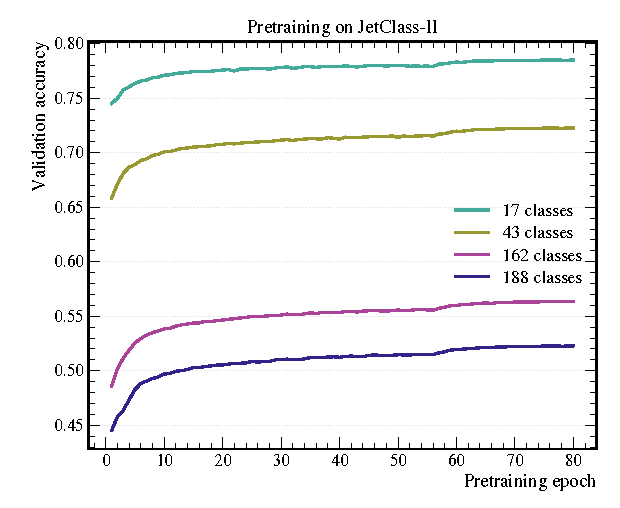
\includegraphics{../../figures/round4/VAL.pdf}
\caption{Every network's pretraining accuracy has levelled off by the last epoch, and the learning-rate decay from epoch 57 adds a small rise to every curve. The curves show the accuracy of each network's own classification output on the JetClass-II validation jets of pretraining against epoch, for 188, 162, 43 and 17 classes and for 162 and 17 classes with an added mass regression (+ mass, lighter shades), the 17 classes + mass curve lying on that of 17 classes. Each network is scored on its own classes, so the heights of the curves do not compare the label sets. Each curve is the mean over the runs of figure 1, and the $\pm$1 standard deviation bands over runs are too narrow to see.}\label{fig:VAL}
\end{figure}
\FloatBarrier
% tables/mlst_inputs.tex
\begin{center}
\begin{minipage}{\linewidth}\centering
\centering
\captionof{table}{The per-particle inputs, with a bullet ($\bullet$) where the top or quark/gluon data provide an input and a dash where they lack it. The last column, for inputs one data set lacks, gives where zero lies after the 188-class network's input normalization, in standard deviations of the pretraining particles (0.00 for the charge and displacements, symmetric about zero). The mean substitution uses the running mean of this input normalization over the pretraining particles. The random-draw substitution gives a top-jet particle a type drawn from JetClass-II's frequencies and a charge given the type, and every particle the displacements of a JetClass-II particle of its type, averaged over four draws. Their results are in table~\ref{tab:fill}. An input marked rescaled is taken after Sophon's rescaling of each jet to $p_{\mathrm{T}}=500$~GeV.}
\label{tab:inputs}
\begin{tabular*}{\linewidth}{@{\extracolsep{\fill}}lccc@{}}
\toprule
input & top & quark/gluon & zero after normalization \\
\midrule
$\log p_{\mathrm{T}}$, rescaled & $\bullet$ & $\bullet$ & -- \\
$\log E$, rescaled & $\bullet$ & $\bullet$ & -- \\
$\log(p_{\mathrm{T}}/p_{\mathrm{T}}^{\mathrm{jet}})$ & $\bullet$ & $\bullet$ & -- \\
$\log(E/E^{\mathrm{jet}})$ & $\bullet$ & $\bullet$ & -- \\
$\Delta R$ & $\bullet$ & $\bullet$ & -- \\
electric charge & -- & $\bullet$ & $0.00$ \\
charged hadron & -- & $\bullet$ & $-0.96$ \\
neutral hadron & -- & $\bullet$ & $-0.35$ \\
photon & -- & $\bullet$ & $-0.81$ \\
electron & -- & $\bullet$ & $-0.10$ \\
muon & -- & $\bullet$ & $-0.08$ \\
$d_0$ & -- & -- & $0.00$ \\
$\sigma_{d_0}$ & -- & -- & $-0.50$ \\
$d_z$ & -- & -- & $0.00$ \\
$\sigma_{d_z}$ & -- & -- & $-0.44$ \\
$\Delta\eta$ & $\bullet$ & $\bullet$ & -- \\
$\Delta\phi$ & $\bullet$ & $\bullet$ & -- \\
\bottomrule
\end{tabular*}
\end{minipage}
\end{center}
\FloatBarrier
% tables/mlst_fill.tex
\begin{landscape}
\begin{center}
\begin{minipage}{\linewidth}\centering
\centering
\captionof{table}{$R_{30}$, the inverse background efficiency at 30\% signal efficiency, of the linear probes of table~\ref{tab:summary} on top and quark/gluon tagging with Pythia jets, with the missing inputs (table~\ref{tab:inputs}) at zero, the training mean (mean) or random draws of a real particle (draws). Table~\ref{tab:summary} uses \LpSubstitutionTop{} for top and \LpSubstitutionQg{} for quark/gluon, so those columns are left out. BatchNorm recomputed means batch-normalization statistics re-estimated on \DesignBnJets{} training jets. The 17-class partitions are in the supplementary material. Values are the mean $\pm$ standard deviation over \MlstNRunsWord{} runs, \MlstMassNRunsWord{} per mass network. Bold marks the best value in their column and those within three standard deviations (run spreads and any stored test-jet bootstrap). The random network is a reference, never bold.}
\label{tab:fill}
\begin{tabular*}{\linewidth}{@{\extracolsep{\fill}}lcccc@{}}
\toprule
 & \multicolumn{2}{c}{top, $R_{30}$} & \multicolumn{2}{c}{quark/gluon (Pythia), $R_{30}$} \\
\cmidrule(lr){2-3}\cmidrule(lr){4-5}
 & zero & mean & zero & draws \\
\midrule
\multicolumn{5}{@{}l}{\textit{linear probe on the frozen features}} \\
\Kfull{} classes & {\fontseries{b}\selectfont 60\,$\pm$\,12} & {\fontseries{b}\selectfont 73\,$\pm$\,15} & {\fontseries{b}\selectfont 66\,$\pm$\,7} & {\fontseries{b}\selectfont 68.1\,$\pm$\,1.8} \\
\Kres{} classes & {\fontseries{b}\selectfont 76\,$\pm$\,17} & {\fontseries{b}\selectfont 64\,$\pm$\,11} & {\fontseries{b}\selectfont 58\,$\pm$\,9} & {\fontseries{b}\selectfont 66.8\,$\pm$\,0.4} \\
\Kres{} classes + mass & {\fontseries{b}\selectfont 86\,$\pm$\,13} & {\fontseries{b}\selectfont 68\,$\pm$\,15} & {\fontseries{b}\selectfont 63.2\,$\pm$\,3.1} & {\fontseries{b}\selectfont 71.3\,$\pm$\,1.1} \\
\Kmid{} classes & {\fontseries{b}\selectfont 57\,$\pm$\,13} & {\fontseries{b}\selectfont 58\,$\pm$\,14} & {\fontseries{b}\selectfont 61\,$\pm$\,9} & {\fontseries{b}\selectfont 69.0\,$\pm$\,1.1} \\
\Kcoarse{} classes & {\fontseries{b}\selectfont 55\,$\pm$\,5} & {\fontseries{b}\selectfont 55\,$\pm$\,5} & {\fontseries{b}\selectfont 62\,$\pm$\,7} & {\fontseries{b}\selectfont 71.6\,$\pm$\,2.8} \\
\Kcoarse{} classes + mass & {\fontseries{b}\selectfont 86\,$\pm$\,24} & {\fontseries{b}\selectfont 68\,$\pm$\,18} & {\fontseries{b}\selectfont 65.79\,$\pm$\,0.31} & {\fontseries{b}\selectfont 73.3\,$\pm$\,2.8} \\
random network, BatchNorm recomputed & 58\,$\pm$\,13 & 60.3\,$\pm$\,2.4 & 54.2\,$\pm$\,2.4 & 52.3\,$\pm$\,0.5 \\
\bottomrule
\end{tabular*}
\end{minipage}
\end{center}
\end{landscape}
\FloatBarrier
% tables/mlst_partrepro.tex
\begin{landscape}
\begin{center}
\begin{minipage}{\linewidth}\centering
\centering
\captionof{table}{The top-tagging training script of the Particle Transformer run from scratch, compared unchanged and with one of two changes taken from Sophon, which are not combined. The changes are Sophon's output head, a 512-unit hidden layer before the output in place of a single linear layer, and its rescaling of each jet to $p_{\mathrm{T}}=500$~GeV. AUC is the area under the receiver operating characteristic curve, $R_{50}$ and $R_{30}$ the inverse background efficiencies at 50\% and 30\% signal efficiency, and the last column counts the background jets passing the $R_{30}$ selection. Table~\ref{tab:published} has the published result and our network from scratch, with both changes. Every value is from a single run, and $R_{30}$, resting on 118 to 165 background jets, has a Poisson uncertainty of 8 to 9\%, larger than the change from Sophon's output head.}
\label{tab:partrepro}
\begin{tabular*}{\linewidth}{@{\extracolsep{\fill}}lccccc@{}}
\toprule
 & accuracy & AUC & $R_{50}$ & $R_{30}$ & background jets passing at $R_{30}$ \\
\midrule
Particle Transformer training script, unchanged & 0.93979 & 0.98585 & 424 & 1{,}710 & 118 \\
the same script with Sophon's output head & 0.94033 & 0.98586 & 416 & 1{,}580 & 128 \\
the same script with Sophon's jet-$p_{\mathrm{T}}$ rescaling & 0.93852 & 0.98504 & 357 & 1{,}220 & 165 \\
\bottomrule
\end{tabular*}
\end{minipage}
\end{center}
\end{landscape}
\FloatBarrier
% tables/mlst_lrsweep.tex
\begin{landscape}
{
\setlength{\LTleft}{0pt}\setlength{\LTright}{0pt}\setlength{\LTcapwidth}{\linewidth}\makeatletter\def\LT@makecaption#1#2#3{\LT@mcol\LT@cols c{\hbox to\z@{\hss\parbox[t]\LTcapwidth{\normalsize #1{#2. }#3\par\vskip\belowcaptionskip}\hss}}}\makeatother
\addtolength{\belowcaptionskip}{\medskipamount}
\begin{longtable}{@{\extracolsep{\fill}}lllcccccccc@{}}
\caption{Learning rates tried for fine-tuning and for training from scratch, at every task and training-set size below the full top-tagging and quark/gluon sets: the best validation accuracy at each rate. Pretrained: the mean over one run each of the networks pretrained with \Kfull{} and \Kcoarse{} classes, the rate being that of the pretrained layers; the new output layer trains at $5\times10^{-3}$ at every rate. From scratch: one run, every weight at that rate. From the earlier rate, rates spaced by factors of about 3 are added until the best one has a lower-scoring rate on each side, and none below $10^{-5}$. Every network of a task and size uses the rate chosen there. $^{\ast}$~marks the rate chosen. ``diverged'': the training loss became non-finite, which counts as lower than any rate that trained; --: not tried.}\label{tab:lrsweep}\\
\toprule
& training jets & & \ensuremath{10^{-5}} & \ensuremath{3\times10^{-5}} & \ensuremath{10^{-4}} & \ensuremath{3\times10^{-4}} & \ensuremath{10^{-3}} & \ensuremath{3\times10^{-3}} & \ensuremath{10^{-2}} & \ensuremath{3\times10^{-2}} \\
\midrule
\endfirsthead
\multicolumn{11}{@{}l}{\textit{Table~\ref{tab:lrsweep} (continued)}} \\[\smallskipamount]
\toprule
& training jets & & \ensuremath{10^{-5}} & \ensuremath{3\times10^{-5}} & \ensuremath{10^{-4}} & \ensuremath{3\times10^{-4}} & \ensuremath{10^{-3}} & \ensuremath{3\times10^{-3}} & \ensuremath{10^{-2}} & \ensuremath{3\times10^{-2}} \\
\midrule
\endhead
top tagging & \ensuremath{10^{3}} & pretrained & -- & -- & -- & \pending{run} & 0.9086 & 0.9068 & 0.9079 & diverged \\
 &  & from scratch & -- & -- & -- & -- & \pending{run} & 0.8831 & \pending{run} & -- \\
 & \ensuremath{10^{4}} & pretrained & -- & -- & -- & -- & -- & 0.9210 & 0.9241$^{\ast}$ & diverged \\
 &  & from scratch & -- & -- & -- & \pending{run} & 0.9174 & 0.9174 & 0.9148 & -- \\
 & \ensuremath{10^{5}} & pretrained & -- & -- & -- & -- & -- & 0.9327 & 0.9332$^{\ast}$ & diverged \\
 &  & from scratch & -- & -- & -- & -- & \pending{run} & 0.9286 & \pending{run} & -- \\
\noalign{\nobreak\vskip\aboverulesep\hrule height\lightrulewidth\nobreak\vskip\belowrulesep\nobreak}
quark/gluon & \ensuremath{10^{3}} & pretrained & -- & -- & 0.7895 & 0.7903$^{\ast}$ & 0.7874 & 0.7840 & 0.7836 & -- \\
 &  & from scratch & 0.7822 & 0.7817 & 0.7826$^{\ast}$ & 0.7705 & 0.7690 & 0.7675 & -- & -- \\
 & \ensuremath{10^{4}} & pretrained & -- & -- & -- & -- & -- & 0.8187 & 0.8214$^{\ast}$ & 0.8205 \\
 &  & from scratch & -- & -- & -- & 0.8050 & 0.8056$^{\ast}$ & 0.8056 & -- & -- \\
 & \ensuremath{10^{5}} & pretrained & -- & -- & -- & \pending{run} & 0.8362 & 0.8360 & 0.8355 & diverged \\
 &  & from scratch & -- & -- & -- & \pending{run} & 0.8266 & \pending{run} & -- & -- \\
\noalign{\nobreak\vskip\aboverulesep\hrule height\lightrulewidth\nobreak\vskip\belowrulesep\nobreak}
JetClass & \ensuremath{10^{4}} & pretrained & -- & -- & -- & \pending{run} & \pending{run} & 0.8088 & 0.7998 & 0.7806 \\
 &  & from scratch & -- & -- & -- & \pending{run} & 0.6836 & \pending{run} & -- & -- \\
 & \ensuremath{10^{5}} & pretrained & -- & -- & -- & -- & \pending{run} & \pending{run} & 0.8266 & \pending{run} \\
 &  & from scratch & -- & -- & -- & \pending{run} & 0.7840 & \pending{run} & -- & -- \\
 & \ensuremath{10^{6}} & pretrained & -- & -- & \pending{run} & \pending{run} & \pending{run} & 0.8403 & 0.8328 & diverged \\
 &  & from scratch & -- & -- & -- & 0.8263 & 0.8294 & 0.8307$^{\ast}$ & diverged & diverged \\
\noalign{\nobreak\vskip\aboverulesep\hrule height\lightrulewidth\nobreak\vskip\belowrulesep\nobreak}
JetClass-II & \ensuremath{10^{4}} & pretrained & -- & -- & 0.3553 & 0.3553 & 0.3665$^{\ast}$ & 0.3654 & 0.3594 & -- \\
 &  & from scratch & -- & -- & -- & 0.1461 & 0.1507 & 0.1608 & 0.1615$^{\ast}$ & diverged \\*
 & \ensuremath{10^{5}} & pretrained & 0.4092 & 0.4123 & 0.4124$^{\ast}$ & 0.4105 & 0.4090 & 0.4060 & 0.3950 & -- \\*
 &  & from scratch & -- & -- & -- & 0.2808 & 0.3020 & 0.3077 & \pending{run} & -- \\*
 & \ensuremath{10^{6}} & pretrained & 0.4290 & \pending{run} & 0.4305 & 0.4293 & 0.4250 & 0.4171 & 0.4048 & -- \\*
 &  & from scratch & -- & -- & -- & 0.3736 & 0.3769 & 0.3812 & \pending{run} & -- \\
\noalign{\nobreak\vskip\aboverulesep\hrule height\heavyrulewidth}
\end{longtable}
}
\end{landscape}
\FloatBarrier
% tables/compute.tex
\begin{landscape}
{
\setlength{\LTleft}{0pt}\setlength{\LTright}{0pt}\setlength{\LTcapwidth}{\linewidth}\makeatletter\def\LT@makecaption#1#2#3{\LT@mcol\LT@cols c{\hbox to\z@{\hss\parbox[t]\LTcapwidth{\normalsize #1{#2. }#3\par\vskip\belowcaptionskip}\hss}}}\makeatother
\begin{longtable}{@{\extracolsep{\fill}}lc>{\raggedright\arraybackslash}p{5.4cm}r>{\raggedright\arraybackslash}p{6.9cm}@{}}
\caption{GPU types and GPU-hours of every pretraining run, summed over the training and validation passes of its epochs as each epoch recorded its device, the GPU types its fine-tuning ran on, and its validation accuracy on its own pretraining classes after the last of its 80 epochs. The last part of the table gives that accuracy as the pretraining-curve figures draw it at the last epoch, the mean $\pm$ standard deviation over \MlstNRunsWord{} runs per label set, \RandFlavRuns{} per flavor-boundary partition and \MlstMassNRunsWord{} per network with an added mass output, and over the five random partitions with one run each. A flavor boundary is a class boundary between decays that differ only in quark flavor. The network pretrained with \Kfull{} classes on the kinematic inputs only has one run and is left out of the last part.}\label{tab:compute}\\
\toprule
network & \begin{tabular}[b]{@{}c@{}}validation\\accuracy\end{tabular} & GPU types (hours) & GPU-hours & fine-tuning GPU types \\
\midrule
\endfirsthead
\multicolumn{5}{@{}l}{\textit{Table~\ref{tab:compute} (continued)}} \\
\toprule
network & \begin{tabular}[b]{@{}c@{}}validation\\accuracy\end{tabular} & GPU types (hours) & GPU-hours & fine-tuning GPU types \\
\midrule
\endhead
\Kfull{} classes, seed 1 & 0.5229 & \mbox{V100 (135)} & 135 & \mbox{L4}, \mbox{L40}, \mbox{RTX 3090}, \mbox{V100} \\
\Kfull{} classes, seed 2 & 0.5226 & \mbox{V100 (145)} & 145 & \mbox{A100 80GB PCIe}, \mbox{L4}, \mbox{RTX 4090}, \mbox{RTX 5000 Ada Generation}, \mbox{TITAN RTX}, \mbox{V100} \\
\Kfull{} classes, seed 3 & 0.5230 & \mbox{RTX 3090 (116)} & 116 & \mbox{A100 80GB SXM4}, \mbox{L4}, \mbox{L40}, \mbox{RTX 5000 Ada Generation}, \mbox{V100} \\
\Kres{} classes, seed 1 & 0.5629 & \mbox{V100 (75)}, \mbox{RTX 3090 (54)} & 129 & \mbox{L4}, \mbox{L40}, \mbox{RTX 3090}, \mbox{RTX 5000 Ada Generation}, \mbox{TITAN RTX}, \mbox{V100} \\
\Kres{} classes, seed 2 & 0.5642 & \mbox{V100 (86)}, \mbox{RTX 3090 (40)} & 126 & \mbox{Quadro RTX 6000}, \mbox{RTX 5000 Ada Generation}, \mbox{V100} \\
\Kres{} classes, seed 3 & 0.5632 & \mbox{V100 (123)}, \mbox{L4 (39)} & 162 & \mbox{L4}, \mbox{Quadro RTX 6000}, \mbox{RTX 3090}, \mbox{TITAN RTX}, \mbox{V100} \\
\Kres{} classes + mass, seed 1 & 0.5579 & \mbox{V100 (129)}, \mbox{RTX 3090 (26)} & 155 & \mbox{L4}, \mbox{Quadro RTX 6000}, \mbox{RTX 3090}, \mbox{RTX 4090}, \mbox{TITAN RTX}, \mbox{V100} \\
\Kres{} classes + mass, seed 2 & 0.5607 & \mbox{V100 (130)}, \mbox{RTX 3090 (15)} & 145 & \mbox{L4}, \mbox{Quadro RTX 6000}, \mbox{RTX 3090}, \mbox{RTX 5000 Ada Generation}, \mbox{TITAN RTX}, \mbox{V100} \\
\Kmid{} classes, seed 1 & 0.7226 & \mbox{RTX 3090 (113)} & 113 & \mbox{L4}, \mbox{Quadro RTX 6000}, \mbox{TITAN RTX}, \mbox{V100} \\
\Kmid{} classes, seed 2 & 0.7226 & \mbox{V100 (101)}, \mbox{RTX 3090 (24)} & 125 & \mbox{L4}, \mbox{Quadro RTX 6000}, \mbox{RTX 3090}, \mbox{RTX 5000 Ada Generation}, \mbox{TITAN RTX}, \mbox{V100} \\
\Kmid{} classes, seed 3 & 0.7231 & \mbox{V100 (107)}, \mbox{RTX 3090 (20)} & 127 & \mbox{L4}, \mbox{L40}, \mbox{Quadro RTX 6000}, \mbox{RTX 3090}, \mbox{V100} \\
\Kcoarse{} classes, seed 1 & 0.7848 & \mbox{RTX 3090 (108)}, \mbox{L4 (3)} & 111 & \mbox{A100 80GB SXM4}, \mbox{L4}, \mbox{L40}, \mbox{RTX 3090}, \mbox{RTX 5000 Ada Generation}, \mbox{V100} \\
\Kcoarse{} classes, seed 2 & 0.7852 & \mbox{V100 (133)} & 133 & \mbox{A100 80GB PCIe}, \mbox{A100 80GB SXM4}, \mbox{L4}, \mbox{RTX 3090}, \mbox{TITAN RTX}, \mbox{V100} \\
\Kcoarse{} classes, seed 3 & 0.7849 & \mbox{V100 (101)}, \mbox{L4 (72)} & 174 & \mbox{A100 40GB PCIe}, \mbox{A100 80GB SXM4}, \mbox{L4}, \mbox{Quadro RTX 6000}, \mbox{RTX 3090}, \mbox{RTX 4090}, \mbox{RTX 5000 Ada Generation}, \mbox{TITAN RTX}, \mbox{V100} \\
\Kcoarse{} classes + mass, seed 1 & 0.7830 & \mbox{V100 (126)}, \mbox{RTX 3090 (16)} & 142 & \mbox{L4}, \mbox{L40}, \mbox{RTX 3090}, \mbox{TITAN RTX}, \mbox{V100} \\
\Kcoarse{} classes + mass, seed 2 & 0.7836 & \mbox{RTX 3090 (101)} & 101 & \mbox{L4}, \mbox{L40}, \mbox{Quadro RTX 6000}, \mbox{RTX 5000 Ada Generation}, \mbox{V100} \\
\multicolumn{5}{@{}l}{\textit{17-class partitions}} \\*
\quad no flavor boundary, seed 1 & 0.7439 & \mbox{RTX 3090 (99)} & 99 & \mbox{A100 80GB PCIe}, \mbox{A100 80GB SXM4}, \mbox{L4}, \mbox{RTX 3090}, \mbox{TITAN RTX}, \mbox{V100} \\*
\quad no flavor boundary, seed 2 & 0.7436 & \mbox{RTX 3090 (130)} & 130 & \mbox{A100 80GB SXM4}, \mbox{L4}, \mbox{Quadro RTX 6000}, \mbox{RTX 4090}, \mbox{RTX 5000 Ada Generation}, \mbox{V100} \\*
\quad $b$-quark boundary, seed 1 & 0.7420 & \mbox{V100 (98)}, \mbox{RTX 3090 (24)} & 122 & \mbox{A100 80GB PCIe}, \mbox{A100 80GB SXM4}, \mbox{L4}, \mbox{Quadro RTX 6000}, \mbox{RTX 3090}, \mbox{TITAN RTX}, \mbox{V100} \\*
\quad $b$-quark boundary, seed 2 & 0.7429 & \mbox{RTX 3090 (137)} & 137 & \mbox{A100 80GB PCIe}, \mbox{A100 80GB SXM4}, \mbox{L4}, \mbox{L40}, \mbox{L40S}, \mbox{Quadro RTX 6000}, \mbox{TITAN RTX}, \mbox{V100} \\*
\quad random flavor boundary, seed 1 & 0.7115 & \mbox{RTX 3090 (125)} & 125 & \mbox{A100 80GB PCIe}, \mbox{L4}, \mbox{RTX 3090}, \mbox{V100} \\*
\quad random flavor boundary, seed 2 & 0.7127 & \mbox{V100 (135)}, \mbox{RTX 3090 (7)} & 142 & \mbox{A100 80GB SXM4}, \mbox{L40}, \mbox{Quadro RTX 6000}, \mbox{RTX 5000 Ada Generation}, \mbox{V100} \\*
\quad random partition 1, seed 1 & 0.6701 & \mbox{RTX 3090 (78)}, \mbox{V100 (38)} & 116 & \mbox{L4}, \mbox{Quadro RTX 6000}, \mbox{RTX 3090}, \mbox{RTX 5000 Ada Generation}, \mbox{V100} \\*
\quad random partition 2, seed 2 & 0.6633 & \mbox{RTX 3090 (110)} & 110 & \mbox{L4}, \mbox{V100} \\*
\quad random partition 3, seed 1 & 0.6692 & \mbox{RTX 3090 (109)} & 109 & \mbox{L4}, \mbox{L40}, \mbox{RTX 3090}, \mbox{V100} \\*
\quad random partition 4, seed 2 & 0.6684 & \mbox{RTX 3090 (107)} & 107 & \mbox{A100 80GB PCIe}, \mbox{L4}, \mbox{RTX 3090}, \mbox{TITAN RTX}, \mbox{V100} \\*
\quad random partition 5, seed 2 & 0.6716 & \mbox{RTX 3090 (98)} & 98 & \mbox{A100 40GB PCIe}, \mbox{A100 80GB PCIe}, \mbox{L4}, \mbox{L40}, \mbox{Quadro RTX 6000}, \mbox{V100} \\*
\Kfull{} classes, kinematic inputs only & 0.2807 & \mbox{RTX 4090 (75)} & 75 & \mbox{A100 40GB PCIe}, \mbox{L40}, \mbox{TITAN RTX}, \mbox{V100} \\
\multicolumn{5}{@{}l}{fine-tuning, every attempt of every cell} \\
\quad of the pretrained networks & -- & \mbox{V100 (2075)}, \mbox{L4 (770)}, \mbox{RTX 3090 (297)}, \mbox{TITAN RTX (210)}, \mbox{A100 80GB PCIe (127)}, \mbox{A100 80GB SXM4 (109)}, \mbox{L40 (99)}, \mbox{RTX 5000 Ada Generation (80)}, \mbox{GPU not recorded (46)}, \mbox{A100 40GB PCIe (43)}, \mbox{Quadro RTX 6000 (27)}, \mbox{RTX 4090 (19)}, \mbox{L40S (4)} & 3{,}906 & -- \\*
\quad from scratch & -- & \mbox{V100 (357)}, \mbox{L4 (105)}, \mbox{TITAN RTX (44)}, \mbox{RTX 3090 (42)}, \mbox{RTX 5000 Ada Generation (25)}, \mbox{L40 (18)}, \mbox{A100 80GB SXM4 (17)}, \mbox{A100 80GB PCIe (15)}, \mbox{RTX 4090 (6)}, \mbox{Quadro RTX 6000 (3)} & 630 & -- \\
\noalign{\nobreak\vskip\aboverulesep\hrule height\heavyrulewidth}
\end{longtable}
\newpage
\noindent\textit{Table~\ref{tab:compute} (continued)}\par\smallskip
\noindent\begin{tabular}{@{}lc@{}}
\toprule
network & \begin{tabular}[b]{@{}c@{}}validation accuracy at the last pretraining epoch,\\mean $\pm$ standard deviation over the runs\end{tabular} \\
\midrule
\Kfull{} classes & 0.52281\,$\pm$\,0.00018 \\
\Kres{} classes & 0.5634\,$\pm$\,0.0007 \\
\Kres{} classes + mass & 0.5593\,$\pm$\,0.0019 \\
\Kmid{} classes & 0.72275\,$\pm$\,0.00027 \\
\Kcoarse{} classes & 0.78497\,$\pm$\,0.00017 \\
\Kcoarse{} classes + mass & 0.7833\,$\pm$\,0.0004 \\
\multicolumn{2}{@{}l}{\textit{17-class partitions}} \\
\quad no flavor boundary & 0.74375\,$\pm$\,0.00025 \\
\quad $b$-quark boundary & 0.7424\,$\pm$\,0.0006 \\
\quad random flavor boundary & 0.7121\,$\pm$\,0.0009 \\
\quad random partitions & 0.6685\,$\pm$\,0.0031 \\
\bottomrule
\end{tabular}
}
\end{landscape}
\FloatBarrier
\end{document}
